


%  \parindent=1.5em


\newacro{SPQR}{Senatus Populusque Romanus}
\newacro{URL}{uniform resource locator}
\newacro{OUP}{Oxford University Press}

\chapter{Acronyms and Abbreviations}


In this section we will discuss the use and typesetting of symbols, abbreviations and acronyms. The |phd| package loads a number of packages and also offers a number of commands in managing symbols, abbreviations and acronyms. The main package we use to manage acronyms is \pkgname{acronym} \cite{acronym}. We also use some build-in commands for abbreviations and to assist in enforcing in-house style guides.

\section{General Principles}

Abbreviations and symbols represent, through a variety of means, a
shortened form of a word or words. Abbreviations fall into three categories:
only the first of these is technically an abbreviation, though the
term loosely covers them all, and guidelines for their use overlap.

\begin{itemize}
\item \textit{Abbreviations} are formed by omitting the end of a word or words (VCR, lbw, Lieut.).
\item \textit{Contractions} are formed by omitting the middle of a word or words (I've,
mustn't, ne'er-do-well
\item \textit{Acronyms} are formed from the initial letters of words (SALT, Nazi, radar), the results being pronounced as words themselves.
\end{itemize}

\section{Acronyms}

An acronym is distinguished from other abbreviated forms by being a series of letters or syllables pronounced as a complete word: \textsc{NATO}
and UEFA are acronyms, but MI6 and BBC are not. Acronyms take no
points, whether all in caps (NAAFI, SALT, WASP), in initial capitals with
upper and lower case (Aga, Fiat, Sogat), or entirely in lower case (derv,
laser, scuba). Since they perform as words they can begin sentences, with
lower-case forms being capitalized normally, such as \textit{Laser treatment}. 

Any all-capital proper-name acronym is, in some house styles, fashioned
with a single initial capital if it exceeds four letters (Basic, Unesco, Unicef).

The \textit{Oxford Guide} suggests that editors should avoid this rule, useful though it is, where the result runs
against the common practice of a discipline (CARPE, SSHRCC, WYSIWYG), or where similar terms would be treated dissimilarly based on length alone.


Acronyms were used in Rome before the Christian era. For example, the official name for the Roman Empire, and the Republic before it, was abbreviated as SPQR (Senatus Populusque Romanus). Inscriptions dating from antiquity, both on stone and on coins, use a lot of abbreviations and acronyms to save room and work. For example, Roman first names, of which there was only a small set, were almost always abbreviated. Common terms were abbreviated too, such as writing just "F" for "filius", meaning "son of", a very common part of memorial inscriptions mentioning people. Grammatical markers were abbreviated or left out entirely if they could be inferred from the rest of the text.\ac{SPQR}

So called \textit{Nomina Sacra} were used in many Greek biblical manuscripts. The common words "God" (Θεός), "Jesus" (Ιησούς), "Christ" (Χριστός), and some others, would be abbreviated by their first and last letters, marked with an overline. This was just one of many kinds of conventional scribal abbreviation, used to reduce the time-consuming workload of the scribe and save on valuable writing materials. The same convention is still commonly used in the inscriptions on religious icons and the stamps used to mark the eucharistic bread in eastern churches.

The early Christians in Rome, most of whom were Greek rather than Latin speakers, used the image of a fish as a symbol for Jesus in part because of an acronym—fish in Greek is ΙΧΘΥΣ (ichthys), which was said to stand for Ἰησοῦς Χριστός Θεοῦ Υἱός Σωτήρ (Iesous CHristos THeou hUios Soter: Jesus Christ, God's Son, Savior). Evidence of this interpretation dates from the 2nd and 3rd centuries and is preserved in the catacombs of Rome. And for centuries, the Church has used the inscription INRI over the crucifix, which stands for the Latin \textit{Iesus Nazarenus Rex Iudaeorum} (``Jesus the Nazarene, King of the Jews'').

The Hebrew language has a long history of formation of acronyms pronounced as words, stretching back many centuries. The Hebrew Bible ("Old Testament") is known as "Tanakh", an acronym composed from the Hebrew initial letters of its three major sections: Torah (five books of Moses), Nevi'im (prophets), and K'tuvim (writings). Many rabbinical figures from the Middle Ages onward are referred to in rabbinical literature by their pronounced acronyms, such as Rambam (aka Maimonides, from the initial letters of his full Hebrew name (Rabbi Moshe ben Maimon) and Rashi (Rabbi Shlomo Yitzkhaki).

The main package we load to assist with acronyms and abbreviations is |acronym|, developed by Tobias Oetiker \citeyearpar{acronym}. The package offers a number of useful commands to help with managing acronyms and to produce lists of acronyms and abbreviations. The package works by offering commands that you use to define an acronym as well as an environment serving the same purpose.

\begin{macro}{\ac}
    To enter an acronym inside the text, use the
\end{macro}
    
    \begin{quote}
     |\ac{|\meta{acronym}|}|
    \end{quote}
    command. The first time you use an acronym, the full name of the
    acronym along with the acronym in brackets will be printed. If you
    specify the |footnote| option while loading the package, the full
    name of the acronym is printed as a footnote.
    The next time you access the acronym only the acronym will
    be printed.

\section{Symbols}

Symbols or signs, are a shorthand notation signifying a word or concept, and are frequent features of scientific and technical writing. The distinction between abbreviation and symbol may be blurred when, lie an abbreviation, a symbol is derived directly from a word or words (\textit{Ag} from \textit{argentum}, \textit{Pa} from \textit{pascal}, \textit{U} from \textit{uranium}), and in setting they are often treated similarly. Unlike abbreviations, however, symbols never take points, even if a single letter, or used alone or in conjuction with figures or words: \textit{F}  for \textit{false}, \textit{fluorine}, \textit{phenylalanine}.

Abstract, purely typographical symbols follow similar rules, being either close up (\ding{38}\ding{33}\ding{43})or spaced (\ding{38} \ding{33} \ding{43}). In \latex you can insert a non-breaking space if you want or a |hairsp|.

|\ding{38}~\ding{33}~\ding{43}|

Personally for the example I would prefer not to split them and the non-breaking space is a better option in this instance.

Symbols' uses can differ between disciplines. For example, in philological
works an asterisk (\textasteriskcentered) prefixed to a word signifies a reconstructed
form; in grammatical works it signifies an incorrect or nonstandard
form. A dagger (\textdagger) may signify an obsolete word, or 'deceased' when
placed before a person's name (this convention should be used only in
relation to Christians). In German a double dagger (\textdaggerdbl) follows the name
and signifies `killed in battle', \textit{gefallen}.

\section{Abbreviations}

\subsection{Time Designations}

Most style guides recommend that you spell out the names of the months in the text but abbreviate them in the list  of works cited, except for May, June and July \cite{MLA}. The same manual suggests that words denoting units of time are also spelled out in the text (\textit{second}, \textit{minute}, \textit{week}, \textit{month}, \textit{year}, \textit{century}, some time designations are used only in the abbreviated form (\textit{a.m., p.m., AD, BC, BC, BCE, CE}). The |phd| package provides some assistance by loading the \pkg{datetime} package; more information on using it and of date and time formatting as well as calculations in Handling Dates and Time can be found in Pages~\pageref{ch:dates}--\pageref{datesend}.
\medskip

\begin{longtable}{lp{8cm}}
AD & after the birth of Christ (from the Latin \textit{anno Domini} `in the year of the Lord'; used before numerals ["\AD 14"] and after references for centuries ["twelfth century \AD"]\\
a.m. & before noon (from the Latin \textit{ante meridiem})\\
Apr. &April\\
Aug. &August\\
BC   &before Christ (used after numerals [``18 BC''] and referenced to centuries [``sixth century BC'']\\
BCE &before the common era (used after numerals and references to centuries)\\
CE  &common era (used after numerals and references to centuries)\\
cent. &century\\
Dec. &December\\
Feb  &February\\
Fri. &Friday\\
hr. &hour\\
Jan. &January\\
Mar. &March\\
min. &minute\\
mo. &month\\
Mon. &Monday\\
Nov. &November\\
Oct. &October\\
p.m. &after noon (from the Latin \textit{post meridiem})\\
Sat. &Saturday\\
sec. &second\\
Sept.&September\\
Sun. &Sunday\\
Thurs. &Thursday\\
Tues. &Tuesday\\
Wed. &Wednesday\\
wk. &week\\
yr. &year\\
\end{longtable}

Tables such as the one above, if not provided by the Publisher, can be very helpful, if you develop them on your own and refer back to them for consistency.

\subsection{Geographic Names}

\subsection{Common Scholarly Abbreviations and Reference Words}

\begin{figure}[tp]
\centering
\fbox{\includegraphics[width=1.0\textwidth]{./images/abbreviations.pdf}}
\caption{A typical Abbreviations page. This has been extracted from \protect\cite{bacchae}.}
\end{figure}


\section{The indefinite article with abbreviations}

The choice between \emph{a} and \emph{an} before an abbreviation depends on pronunciation,
not spelling. Use a before abbreviations beginning with a
consonant sound, including an aspirated h and a vowel pronounced with the sound of w or y.

\begin{scriptexample}
a BA degree a KLM flight a BBC announcer
a Herts, address a hilac demonstration a YMCA bed
a SEATO delegate a U-boat captain a UNICEF card
\end{scriptexample}

Use \emph{an} before abbreviations beginning with a vowel sound, including
unaspirated \emph{h}:

an AB degree an MCC ruling an FA cup match
an H-bomb an IOU an MP
an MA an RAC badge an SOS signal

This distinction assumes the reader will pronounce the sounds of the
letters, rather than the words they stand for (a Football Association cup
match, a hydrogen bomb). MS for manuscript is normally pronounced as
the full word, manuscript, and so takes a; MS for multiple sclerosis is
often pronounced em-ess, and so takes an. Likewise 'R.' for rabbi is
pronounced as rabbi ('a R. Shimon wrote'), but 'R' for a restricted classification
is normally pronounced as arr ('an R film').

The difference between sounding and spelling letters is equally important
when choosing the article for abbreviations that are acronyms and
for those that are not: a NASA launch but an NAMB award. The same holds
for names of symbols, which can vary: in America a hash symbol (\#) is a
'number sign' or, more formally, an \textit{octothorp}; in linguistic use an
asterisk may be called a 'star' and in mathematics an exclamation
mark called a 'factorial', 'shriek', or 'bang', so the correct forms are a *
and a ! rather than an * and an !. 

As abbreviated terms enter the
language there can be a period of confusion as to how they are pronounced:
in computing, for example, \ac{URL} is
pronounced by some as an abbreviation (you-are-ell) and others as an
acronym (earl), with the result that some write it as a URL and others as
an URL. Until a single pronunciation becomes generally accepted, the
best practice is simply to ensure consistency within a given work.

\section{Latin abbreviations}
\normalfont

Do not confuse 'e.g.' (\emph{exempli gratia}), meaning 'for example', with 'i.e.'
{id est), meaning 'that is'. Compare hand tools, e.g. hammer and screwdriver
with hand tools, \ie those able to be held in the user's hands. Print both lower-case roman, with two points and no spaces, and preceded by a
comma. In OUP style 'e.g.' and 'i.e.' are not followed by commas, to avoid
double punctuation; commas are often used in US practice.

Although many people employ 'e.g.' and 'i.e.' quite naturally in speech
as well as writing, prefer 'for example' and 'that is' in running text.
(Since 'e.g.' and 'i.e.' are prone to overuse in text, this convention helps
to limit their profusion.) Conversely, adopt 'e.g.' and 'i.e.' within parentheses
or notes, since abbreviations are preferred there. A sentence in text cannot begin with 'e.g.' or 'i.e.'; however, a note can, in which case
they—exceptionally—remain lower case. The \textit{Oxford Guide} gives an example of exception to the rule

The package offers two commands:

\begin{verbatim}
\newcommand{\ie}{\textit{i.\hairsp{}e.}\xspace}
\newcommand{\eg}{\textit{e.\hairsp{}g.}\xspace}
\end{verbatim}

The commands handle the spacing and if they are to be in italics or not. Renew the commands to set the style you want.

\section{Units}
\label{units}

Most users of \latex will have a need for specifying units in  mathematical or text contexts. We load the \pkgname{siunitx} package. The package was developed by Joseph Wright\cite{siunitx}. The correct application of units of measurement is very important in technical applications. For this reason, carefully-crafted definitions of a coherent units system have been
laid down by the \textit{Conférence Générale des Poids} et Mesures (CGPM): this has resulted in
the \textit{Système International d’Unités} (SI). At the same time, typographic conventions for
correctly displaying both numbers and units exist to ensure that no loss of meaning
occurs in printed matter.

|siunitx| aims to provide a unified method for \latex users to typeset numbers and
units correctly and easily. The design philosophy of |siunitx| is to follow the agreed rules
by default, but to allow variation through option settings. In this way, users can use
|siunitx| to follow the requirements of publishers, co-authors, universities, etc. without needing to alter the input at all.



\makeatletter
\ExplSyntaxOn
\box_new:N \g_@@_syntax_box
\newenvironment{syntax}
 {
  \small\ttfamily
  \bool_if:NTF \l_@@_long_name_bool
    {
     \hbox_gset:Nw \g_@@_syntax_box
     \arrayrulecolor{white}
     \begin{tabular}{@{}l@{}}
     \toprule
     \begin{minipage}
       { \textwidth+0.75\marginparwidth-\l_@@_trial_width_dim }
    }
    {
     \hbox_gset:Nw \g_@@_syntax_box
     \arrayrulecolor{white}
     \begin{tabular}{@{}l@{}}
     \toprule
     \begin{minipage}{ \textwidth }
    }
  \raggedright
  \obeyspaces\obeylines
 }
 {
  \end{minipage}
  \end{tabular}
  \arrayrulecolor{black}
  \hbox_set_end:
  \ignorespacesafterend
 }

\newenvironment {ddanger}
 {
  \begin{trivlist}\item[]\noindent
  \begingroup\hangindent=3.5pc\hangafter=-2
  \cs_set_nopar:Npn \par{\endgraf\endgroup}
  \hbox to0pt{\hskip-\hangindent\dbend\kern2pt\dbend\hfill}\ignorespaces
 }{
  \par\end{trivlist}
 }
\ExplSyntaxOff

\begin{ddanger}
Angles can be typeset using the \cs{ang} command.  The
 \meta{angle} can be given either as a decimal number or as a
 semi-colon separated list of degrees, minutes and seconds, which
 is called \enquote{arc format} in this document. The numbers which
 make up an angle are processed using the same system as other numbers.
\end{ddanger}

%  

\chapter{Boxes and glue in TeX}

\setlength{\columnsep}{2em}
{\it Once you understand TEX's concept of glue, you may well decide that
it was misnamed; real glue doesn't stretch or shrink in such ways, nor does it
contribute much space between boxes that it welds together. Another word like
\emph{spring} would be much closer to the essential idea, since springs have a natural
width, and since different springs compress and expand at different rates
under tension. But whenever the author has suggested changing \tex's terminology,
numerous people have said that they like the word \emph{glue} in spite of its
inappropriateness; so the original name has stuck. }
\smallskip

{\hfill  ---  Donald E. Knuth}

\medskip   


\parindent1em




\newthought{Traditional typesetting} was a task that depended on assembling the types and inserting them one by one on holding frames. In a way it was an assembly of boxes.
The \tex typesetting system uses a similar model of boxes to typeset content but in addition it also uses the concept of glue to stretch or shrink the text so that it will look better typographically. Boxes contain
typeset objects, such as text, mathematical displays, and pictures, and glue
is flexible space that can stretch and/or shrink by amounts that are under
user control.

\topline

Some example is placed her\\
and

\bottomline

\section*{Boxes}

Boxes in \tex have  a rectangular shape but have
three associated measurements called \emph{height}, \emph{width}, and \emph{depth}.
Figure \ref{fig:boxes} shows a 
picture of a typical box, showing its so-called \emph{reference point} and \emph{baseline}

The reason that they have three dimensions is that a character of text has normally three dimensions as shown in figure \ref{fig:boxes}. As characters need to be lined on a baseline, the depth provides a datum point on which they can be aligned and the depth provides a measure of the portion of the character that is below the baseline.


Boxes and glue are the main tools of \tex. The box can hold text and other items. Glue is simply spacing. It can be horizontal or veritcal spacing, and it can be made as rigid or as flexible as desired.



\begin{minipage}{\linewidth}
\textbf{One important feature of \tex is that it has no knowledge of the shape of the characters it typesets, just the dimensions of each character box.}
\end{minipage}
\medskip

When \tex is typesetting, it is normally in horizontal mode, such as while
it is working on this paragraph. Otherwise, \tex can be in vertical mode, or
in math mode, or three others described in Chapter 13 of The \texbook.
Two low-level TEX commands for boxes are \cmd{hbox}, for a horizontal box,
and \cmd{vbox} for a box in vertical mode. In the latter, \tex is normally still
collecting material for display from right to left: it is not building up a
column of text, as in classical Chinese writing.

In both kinds of boxes, the result is an unbreakable object that acts
much like a single character. \tex reads input as a string of characters,
then breaks that string up in words, each of which forms a box. 
\emph{Word boxes}\index{word boxes}
are then collected into lines, lines into paragraphs, and paragraphs into a
page galley. The space between the words can be normal \emph{interword space},
or \emph{sentence-ending} space, which is somewhat larger in English-language
typesetting, and the space is normally glue, rather than of fixed size.

\tex has a sophisticated mathematical algorithm for figuring out the
best way to stretch or shrink interbox glue to optimize the appearance of
lines and paragraphs. Every so often, \tex checks to see whether it has
enough material saved on the growing page galley to fill a complete output
page, and it asynchronously (and effectively, unpredictably) calls the
output routine whose job it is to figure out where the page break should
happen, ship out a completed page to the |DVI|  file, and replace the galley by
whatever is left over.

In traditional \tex you  can force a line break with the carriage-return command \cmd{cr},
and a page break with the command \cmd{eject}, but \tex is an expert system,
and normally handles line and page breaking on its own. \latex provides its own commands such as \cmd{clearpage} and \cmd{newpage} and so do all other \tex based systems.

\latex does not modify any of \tex's algorithms but simply it is a set of implemenation
macros.

\section{Units of measurement in TEX}

\tex allows you to specify sizes of typographical objects in any of nine different
units:


\begin{table}[htbp]
\begin{center}
\begin{tabular}{llp{5cm}}
\toprule
bp &big point &1 inch is exactly 72 bp; the PostScript pagedescription language uses these units, but just calls them points\\
cc &cicero: &1 cc is exactly 12 didot points, and is thus the European  analogue of the pica\\
cm &centimeter: &1 in is exactly 2.54 cm\\
dd &didot point: &1 dd is (1238/1157) pt, and is a typographical unit common in some parts of Europe\\
in &inch: &an archaic unit, roughly the width of a man's thumb; it has been discarded by most countries, but still used in the USA and its sattelites.\\
mm &millimeter: &1 in is exactly 25.4 mm\\
pc &pica: &1 pc is exactly 12 pt\\
pt &printer's point: &1 in is exactly 72.27 pt\\ 
sp &scaled point: &1 pt is exactly $2^{16}$ = 65536 sp.\\
\bottomrule
\end{tabular}
\end{center}
\end{table}



The units can be separated from their numeric value with optional space, so
\texttt{3pc} and \verb*+3 pc+ are equivalent. The little half box in the latter is a convenient
way to indicate explicit spaces in typewriter text. It can be printed by typing \cmd{char32}.

Internally, \tex\ stores dimensions as integral numbers of scaled points:
1 sp is tiny ---  smaller than the wavelength of visible light.\footnote{The visible light has wavelengths from 380--450 nm for violet up to 620--750 nm for red (sp = 280 nm} It is sometimes
useful to create objects that small so that they differ from empty objects,
but are nevertheless invisible. It also ensures that TeX will look the same irrespective on which computer you actually compiled your document.

\tex deals only with 32-bit integer words, and does not take advantage
of extra precision available on historical machines with larger words. The
lower 16 bits of a dimension can be viewed as a fractional number of points,
and the uppermost bit is needed for a sign (0 for plus, 1 for minus). That
leaves 15 bits to hold an integral number of points, but TEX only expects 14
to be used, so that addition of two dimensions does not overflow. Thus, the
largest dimension in TEX is exactly 214 + (1 26) points, or about 5.758  
meters or 18.89 feet.

\tex has several kinds of special storage locations, called registers, numbered
from 0 to 255. For example,\cs{dimen0} can hold a fixed dimension,
which can be specified in any of the nine units of measurement that are
recognized by \tex.

Here is how you can assign a dimension to a register, and then have \tex
display it back for you:

\begin{teXXX}
\dimen1 = 25.4mm (*@\protect\footnote{You shouldn't assign dimenensions to primitive registers, but rather use one of the allocation schemes provided by LaTeX to do so.}  @*)
\the\dimen1
\end{teXXX}

This will result in
\dimen1 = 25.4mm

\the\dimen1


Notice that \tex’s output is always in points, showing that it converts different
input units to a common system of measurement.

You can convert a dimension to the much-smaller units of scaled points
by assigning it to another kind of \tex register designed to hold signed integers,
the\cs{count0} through\cs{count255} registers:

\begin{texexample}{}{}
\dimen4 = 1pt
\count4 = \dimen4
\the\count4
\end{texexample}

{\noindent This time we get the size as \texttt{sp} as 65536 }


You might have noticed that the conversion from inches to points was not
quite what we claimed in the summary of \tex units. Here is how to see the
differences:

\verb+\dimen1 = 1in+


\section{Skip registers}
\index{registers!skip}
\begin{macro}{\skip}
\tex glue is specified as a fixed dimension, and optionally, with a plus and/
or minus dimension. Along with \cs{dimen} registers, TEX has glue registers,
called \cs{skip0} through \cs{skip255}. Here is how you can save glue settings in
 registers, and ask \tex to display the contents of one of them:
\end{macro}

\begin{teXXX}
  \skip1 = 10pt
  \skip2 = 10pt plus 3pt
  \skip3 = 10pt minus 2pt
  \skip4 = 10dd plus 3dd minus 2dd
  \showthe \skip4
  > 10.70007pt plus 3.21002pt minus 2.14001pt.
\end{teXXX}


The four sample glue settings store, respectively, \textit{fixed glue}, \textit{stretchable
glue}, \textit{shrinkable glue}, and \textit{flexible glue} that can both stretch and shrink,
but only up to a specified amount. Interword and intersentence spaces are
generally defined with glue like this, so that if more stretch or shrink of
\index{glue}\index{glue!flexibe}\index{glue!stretchable}\index{glue!shrinkable}

\begin{teX}
\dimen2 = 72.27pt
\count1 = \dimen1
\count2 = \dimen2
\showthe \count1
> 4736286.
\showthe \count2
> 4736287.
\end{teX}

The two values differ by the tiny value 1 \textit{sp}, so we can in practice ignore
that difference. If we use higher-precision arithmetic, we find the exact
decimal equivalents of the fractions as

\begin{teX}
4 736 286=65 536 = 72.269 989 013 671 875;
4 736 287=65 536 = 72.270 004 272 460 937 5;
4 736 286.72=65 536 = 72.27
\end{teX}


Actually \tex uses that last relation as the definition of the conversion of
inches to scaled points, so that our assignment of 1 in to \verb+\dimen1+ has to
be rounded to the nearest integral number of scaled points. That is why
in the round-trip conversion from decimal to binary and back to decimal,
1 in became 72.26999 pt. \tex guarantees that its output decimal numbers
are always converted on input back to the original binary numbers from
whence they came. For more on the story of \tex’s I/O conversions, see [3].


Both \tex and \latex define a number of predefined dimensions and these are discussed in the relevant Chapters discussing the \latex kernel. For example you might have come across the \cs{jot}, which is defined by \latex as:

\begin{teXX}
\newdimen\jot
This is some sample text with a one |\jot| left indentation. Which is really too small to see in a paragraph.
\jot=3pt
\end{teXX}

Defining |\parindent=jot| we can see that the indentation almost disappeared. This is obvious since |\jot| is used normally for maths.

Glue is the binder that lets \tex\ do its job. This chapter discusses some
preset forms of glue and their uses. Along with glue parameters there are a
number of special commands for inserting glue. The most interesting have
different degrees of infinity, namely |\hfil|, |\hfill|, |\hfilneg|, |\hss|,
and their vertical counterparts. 

Because of the special spacing requirements of mathematics, \tex\ defines
skips and spacing that are valid in mathematics mode only. Examples are the
are the special preset |mu| glues of |\thickmuskip|,
|\medmuskip|, |\thinmuskip|.
The |\newskip| and |\newmuskip| commands allocate skip (or really glue)
or muskip registers respectively for special uses. For example the specific
glues surrounding section heads are held in glue registers. 

It should be noted that the various |\...muskip| do not cause horizontal
spacing in math mode by themselves. They are used with |\mskip| to actually
cause the insertion of the glue.

These are all various forms of horizontal (or math) mode commands that insert
infinite quantities of glue. |\hfil|, |\hfill|, |\hfilneg|, and |\hss| insert
|plus 1fil|, |plus 1fill|, |minus 1fil|, and |plus 1fil minus 1fil|. 
The first two are {\it stretch} glues, the third is {\it shrink} glue and the
last is both. It
should be noted that when \tex\ tries to stretch or shrink glue values, they
vary according to their value. If there exists both |fil| and finite value
glue in a box or line, then all the stretch if it is |plus| glue 
or shrink if it is |minus| glue will be in
the section with the |fil| glue. If there is |fill| glue and either |fil| or
finite glue, then all the stretch or shrink will be in the |fill| sections.
Similarly with |filll| glue, which is not supplied in as readily usable form.
The difference in behaviour between |\hfil| and |\hss| is that |\hss| glue
will allow the contents of a box to spill outside without resulting in an
overfull box while |\hfil| will only fill or push contents to the edge of the
box. The major use for these glues are to center or to force stuff to either
edge of a box.  For instance this

\begin{texexample}{}{}
\def\aline{\vrule \hfil one \hfil two \hfil three 
         \hfill four \hfil five \hfil six 
         \hfill seven \hfil eight \hfil nine\vrule}

\aline

This is a preset |mu| glue. |\medmuskip = 4mu plus 2mu minus 4mu| for use
with |\mskip|. This is \hbox{\strut\vrule$\mskip\medmuskip$\vrule}.
\end{texexample}


\begin{macro}{\newskip}
The command \cs{newskip}\meta{skip name} assigns a new skip or glue register to
the name |\<skip name>|. Glue values may be assigned to it by |\<skip name> [=] <glue>|.
This assigns a new muskip or muglue register to the name |\<muskip name>|. Glue
values may be assigned to it by |\<muskip name> [=] <muglue>|.

This is a preset |mu| glue. |\thickmuskip = 5mu plus 5mu| for use
with |\mskip|. This is \hbox{\strut\vrule$\mskip\thickmuskip$\vrule}.

This is a preset |mu| glue. |\thinmuskip = 3mu| for use
with |\mskip|. This is \hbox{\strut\vrule$\mskip\thinmuskip$\vrule}
\end{macro}


\newskip\hides 
\hides= -1000pt% plus 1fill

atest atest

\hskip\hides atest

\hides= -1000pt  plus 1fill

atest atest

\hskip\hides atest

|\vfil \vfill|

|\vfilneg|

|\vss|

These are the vertical analogues to the infinite horizontal glues and act in
much the same manner. See the section on |\hfil ...|.
 



\normalsize



\section{Glue}

\tex joins the boxes it creates with some special mortar as Knuth writes, called glue. To understand how glue works we will
borrow a figure from the \tex Book.

\begin{figure}
  \centering
  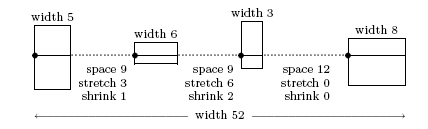
\includegraphics[width=0.9\linewidth]{./images/glue.png}
  \caption{Glue in \TeX}
  \label{fig:glue}
\end{figure}


\section{How to specify glue}

The usual way to specify \textit{glue} to \tex is
$<dimen>< plus~dimen><minus~dimen>$

where the plus and minus are optional and assumed to be zero if not
present; plus\index{glue!plus} introduces the amount of stretchability\index{glue!stretchability}, minus introduces the amount of shrinkability \index{glue!shrinkability}. 

For example, Appendix B of the TexBook defines \cs{medskip} to be an abbreviation for
|\vskip6pt plus2pt minus2p|. The normal-space component of glue must always be
given as an explicit dimen, even when it is zero. The ability of \TeX to stretch and shrink this glue has given it its beautiful looks. Strangely enough, although the algorithm is public it has not been used widely in other software.



\subsection*{hfil and hfill}

{\obeylines
{This text will be flush left.\hfil}
{\hfil This text will be flush right.}
{\hfil This text will be centered.\hfil}
{Some text flush left\hfil and some flush right.}
{Alpha\hfil centered between Alpha and Omega\hfil Omega}
{Five\hfil words\hfil equally\hfil spaced\hfil out.}
}

Consider the following definitions:

\begin{verbatim}
\def\centerlinea#1{\hfil#1\hfill}
\def\centerlineb#1{\hfill#1\hfill}
\def\centerlinec#1{\hss#1\hss}
We define quickly a \cs{lineX}\footnote{Strange but my \LaTeX\ distribution has not got on. (This definition is from \texttt{plain.sty}}

\def\lineX{\hbox to\hsize}
\def\lineX{\hbox to\hsize}
\def\centerlinea#1{\hfil#1\hfil}
\def\centerlineb#1{\hfill#1\hfill}
\def\centerlinec#1{\hss#1\hss}

\lineX{\centerlinea{\test}}
\lineX{\centerlineb{\test}}
\lineX{\centerlinec{\test}}
\centerline{\test}
\begin{center}\test\end{center}

\end{verbatim}


\section{Specifying glue amounts}

\tex glue is specified as a fixed dimension, and optionally, with a plus and
or minus dimension. Along with \cs{dimen} registers, TEX has glue registers,
called \cs{skip0} through \cs{skip255}. Here is how you can save glue settings in
\tex registers, and ask \tex to display the contents of one of them:

\begin{teX}
\skip1 = 10pt
\skip2 = 10pt plus 3pt
\skip3 = 10pt minus 2pt
\skip4 = 10dd plus 3dd minus 2dd
\the \skip4
\end{teX}


\texttt{> 10.70007pt plus 3.21002pt minus 2.14001pt}

The four sample glue settings store, respectively, {\em fixed glue}, {\em  stretchable
glue}, {\em shrinkable glue}, and {\em flexible glue}  that can both stretch and shrink,
but only up to a specified amount. Interword and intersentence spaces are
generally defined with glue like this, so that if more stretch or shrink of  a
re underfull (too little text to fill the line), or overfull (too much text in the
line).



\section{Overfull lines}

Although overfull lines are reported in the \tex log file, they can be hard
to find in the typeset document if they only stick out a little. To make
them highly visible while you are fine tuning your final document, assign
the variable \cs{overfullrule} a nonzero dimension, such as 2 cm. \tex then
displays a solid black box, called a \emph{rule}, of that width in the right margin
on each line that is overfull. Using the \docpkg{microtype} package one can adjust the parameters to minimize this.

To make the rules disappear, simply remove it,
or comment out, the assignment, or reset its value to 0 pt. 

Just as you can assign dimension registers to count registers to convert
from points to scaled points, you can assign skip registers to dimension and
count registers to discard the flexible parts:


\begin{teX}
\skip1 = 10pt plus 3pt minus 2pt
\the\skip1
 \dimen1 = \skip1
\the \dimen1
\count1 = \skip1
\the \count1
\end{teX}




\section{More on glue in boxes}

Besides normal glue with fixed amounts of stretch and shrink, \tex also has
two kinds of glue that are \emph{infinitely} stretchable and shrinkable: \cs{hfil} and
\cs{hfill} in horizontal mode, and \cs{vfil} and \cs{vfill} in vertical mode. Notice that there two versions
of the commands, the one ends with one ell and the second one with two. The
two-ell forms are more flexible than the one-ell forms.

The boxes and glue model is powerful, and \tex's author, Donald Knuth,
has written that he views it as the key idea that he discovered when he
first sat down in 1977--1978 to design a computer program for typesetting.
For example, to set something flush left, put infinitely-stretchable glue on
its right. To set it flush right, put the glue on the left. For centered material,
put the glue on both sides. Here are four examples, with vertical
bars marking the ends of the horizontal box (boxes have no visible frames,
although it is possible to write \tex commands to give them such outlines,
and we use that feature shortly):





\section{Horizontal and vertical boxes}


\noindent \lettrine{L}{ike} their dimensions \TeX's boxes are not what one thinks when thinking of boxes. TeX's boxes come in basically two flavours, horizontal boxes and vertical boxes. An \cs{hbox} is created by the command |\hbox{material}|. It has the following properties:

\begin{enumerate}
\item The material is placed from left to right and it becomes a \textit{horizontal list}.\index{horizontal list}
\item The box \textbf{cannot be broken across lines}; it is an indivisible unit.
\end{enumerate}

An |hbox| can contain, characters, horizontal glue, horizontal leaders or other boxes. While in many cases these other boxes can be other |\hbox|es, |\vbox| can be used.

Boxes can be moved up or down using |\raise| or |\lower|. Each of these primitives is followed by a dimension indicating how far the box can be lowered or raised.

Other material that can go in an hbox, is \textbf{vertical rules}. 

\subsection{The null macro}

The |\null| macro is defined both in Plain as well as LaTeX and generates an empty box. Its definition is:

\begin{teXXX}
\def\null{\hbox{}}
\end{teXXX}


\fbox{\hbox{This is a test}}

{
\fbox{\hsize=5cm
A test of a box at the end of a 2.0 inch line\par}

\fbox{\hsize=5.0cm in A test of a box at the end of a \hbox to 2cm{2.0 cm} line\par}

}

What happens when we have more than two boxes on a line? TeX will stuck them one under another. If they are enclosed within another hbox they will be inlined.



\begin{texexample}{}{}
\hbox to 1cm {A} \hbox to 1cm {B}

If we however, put them together in another |\hbox|, we get:

\hbox{\hbox to 1cm {A} \hbox to 1cm{B}}
\end{texexample}




An |\hbox| does not imply horizontal mode, so an attempt to start a paragraph with a box, for
instance
|\hbox to 0cm{\hss$\bullet$\hskip1em}Text ...|

will make the text following the box wind up one line below the box. It is necessary to switch
to horizontal mode explicitly, using for instance |\noindent| or |\leavevmode|. The latter is defined
using |\unhbox|, which is a horizontal command.


\begin{texexample}{}{}
\hbox to 0cm{\hss$\bullet$\hskip1em} Text ...


\leavevmode\hbox to 0cm{\hss$\bullet$\hskip1em} Text ...

\end{texexample}




\section{Kerning}

\begin{multicols}{2}
Using the command \cs{kern}, we can move boxes either left or right. Kerning is extensively used to build internal commands and we discuss it in more detail under the chapter for fonts.

Consider two horizontal boxes, holding the letters A and V:
As you can observe, the letters AB are a bit afar, from what would be a visually pleasant arrangement, we can kern them as follows:
\medskip
\begin{teXXX}
\hbox{\Huge AV A\kern-5ptV}
\end{teXXX}
\medskip
Note that hbox, does not produce a frame. I~have used a frame |\fbox|, which will cover a bit later as well as scaled the image by 2, in order to see the effects more clearly.
\columnbreak

\centerline{\scalebox{2}{\hbox{\hbox{\huge A}\hbox{\huge V}}} \scalebox{2}{\hbox{\hbox{\huge A}\kern-5pt\hbox{\huge V}}}}
\end{multicols}




\noindent\begin{tabular}{ll}
|\hbox{\kern4pt A\kern8pt B\kern8pt C\kern4pt}| & \fbox{\hbox{\kern4pt A\kern8pt B\kern8pt C\kern4pt}} \\
~ &\\
\midrule
|\hbox{\kern4pt\raise1pt\hbox{A}|  & \fbox{\hbox{\kern4pt\raise1pt\hbox{A} \kern8pt BC\kern8pt\lower6pt\hbox{D} \kern4pt} \kern8pt BC\kern8pt\lower6pt\hbox{D}\kern4pt} \\
|\kern8pt BC|                      &\\
|\kern8pt\lower6pt\hbox{D}|        &\\
|\kern4pt}|                        &\\ 
|\kern8pt BC|                      &\\ 
|\kern8pt\lower6pt\hbox{D}|        &\\
|\kern4pt}| &\\
\midrule
\end{tabular}


\vbox{
\noindent\rule{\linewidth}{0.4pt}
\begin{minipage}{4.5cm}
 \begin{teXX}
\fbox{\hbox{\kern4pt A\kern8pt 
      B\kern8pt C\kern4pt}}
\end{teXX}
\end{minipage}
\hfill\hfill
\begin{minipage}{3cm}
\hfill\hfill\fbox{\hbox{\kern4pt A\kern8pt 
      B\kern8pt C\kern4pt}}
\end{minipage}

\medskip
\noindent\rule{\linewidth}{0.4pt}
}

Notice that an |\hbox| is constructed by setting its components side by side so that their \textit{baselines} are aligned. When \cs{raise}, \cs{lower} are used the baselines are no longer aligned. In such a case the baseline of the box is defined as the baseline shared by the components before any vertical movements. In the example above the box now has a depth, as a result of lowering |D|.


\vbox{
\noindent\rule{\linewidth}{0.4pt}
\begin{minipage}{4.5cm}
\begin{teXXX}
\hbox{\kern4pt\raise1pt\hbox{A} 
  \kern8pt BC\kern8pt
  \lower6pt\hbox{D} 
  \kern4pt} 
\end{teXXX}
\end{minipage}
\hfill
\begin{minipage}{3cm}
\fbox{\hbox{\kern4pt\raise1pt\hbox{A} 
\kern8pt BC\kern8pt\lower6pt\hbox{D} \kern4pt}}
\end{minipage}

\medskip
\noindent\rule{\linewidth}{0.4pt}
}

\clearpage

\begin{multicols}{2}
\noindent\textbf{Vertical boxes.}\quad A vertical box is build in a similar manner to that of a horizontal list, except it is composed of material in the \textit{vertical list}.
When horizontal boxes are added in the list, they are stuck on top of each other as shown in the example below. 
\medskip
\begin{teXXX}
\vbox{\hsize=0.8cm\hbox{A} \hbox{AB}} 
\end{teXXX}
\columnbreak

\parindent0pt
\fbox{\vbox{\hsize=3cm\fbox{\hbox{ABCDEFGH}} \fbox{\hbox{AB}}}}
\end{multicols}

\begin{multicols}{2}
It is important to remember the two main differences between hboxes and vboxes. An hbox will expand to hold its material. If it need be it will overfill the line and produce an overful warning. A vbox will expand to hold its material. It is perfectly normal for a vbox to hold paragraphs, as shown. This is not possible with an hbox.

\columnbreak

\noindent\fbox{\vbox{\lorem\par\lorem\par}}
\end{multicols}



\topline
\begin{multicols}{2}
\noindent\textbf{Controlling the size of a vbox.}\quad What controls the size, is the containing environment. This in TeX, is specified using |\hsize|. In LaTeX this is controlled by an enclosing environment, maybe a minipage (which is build this way) or one of the page width parameters.
\end{multicols}



\begingroup
\parindent0pt
\fboxsep5pt
\hsize=3.8cm\footnotesize
\hfil\fbox{\vbox{\lorem\par}} 
\hfil\fbox{\vbox{\lorem\par}}
\hfil\fbox{\vbox{\lorem\par}}\hfill
\endgroup
\captionof{figure}{Output to demonstrate the use of vboxes.}


\begin{multicols}{2}
The code to typest the boxes shown above follows:
\medskip
\emphasis{hsize}
\begin{teXXX}
\bgroup
\parindent0pt
\hsize=3.3cm\footnotesize
\hfil\fbox{\vbox{\lorem\par}} 
\hfil\fbox{\vbox{\lorem\par}}
\hfil\fbox{\vbox{\lorem\par}}
\hfill
\egroup
\end{teXXX}
\columnbreak

Note, the use of hsize. We define the font size as |\footnotesize|. We have done this in order not to have overfull boxes--Latin words don't have a full set of hyphenation patterns in \latex. The macro |\lorem|, we have defined internally for this document. We place the code in a group in order not to affect the rest of the document.
\end{multicols}


\clearpage

\noindent\textbf{Vertical centering}\quad can be achieved by applying vertical infinite glue \cs{vfill}. In the example that follows, first we place two letters in individual |\hboxes| and we enclose them in a vbox. We apply |\vfill| both on top and at bottom.

\emphasis{\vfill}

\vbox{
\noindent\rule{\linewidth}{0.4pt}
\begin{minipage}{5cm}
\begin{teX}
\fbox{\vbox to 0.9cm{\vfil\hbox{M}\nointerlineskip\hbox{i}\vfil}} 
\end{teX}
\end{minipage}
\hfill
\begin{minipage}{3cm}
\hfill\fbox{\vbox to 0.9cm{\vfil\hbox{M}\nointerlineskip\hbox{i}\vfil}}\hfill\hfill 
\end{minipage}

\medskip
\noindent\rule{\linewidth}{0.4pt}
}



A |\vbox| can be combined with text and may appear anywhere within a paragraph. The baseline of the box will be aligned with the baseline of the current line.


\vbox{%
\noindent\rule{\linewidth}{0.4pt}}

\begin{teX}
A vbox can be placed within a paragraph \fbox{\vbox to 0.6cm{\vfil\hbox{M}\nointerlineskip\hbox{i}\vfil}} as shown here.


\hfill

A vbox can be placed within a paragraph \fbox{\vbox to 0.6cm{\vfil\hbox{M}
  \nointerlineskip\hbox{i}\vfil}} as shown here.

\end{teX}

\medskip
\noindent\rule{\linewidth}{0.4pt}






\noindent\textbf{Top alignment.}\quad\cs{vtop} is similar to a |\vbox|. The depth of this box is zero, since both A and B are capital letters. The width of this box is |\hsize|, since it contains text. 


\begin{codeexample}[]
\vtop{\hbox{A} \hbox{B}}
\end{codeexample}






Centering a picture in a box, both vertically and horizontally can be achieved using the methods we described so far.


\emphasis{hfill,hbox}
\begin{texexample}{}{}
     \fbox{%
          \vtop{\medskip
                    \hfill
                      \hbox{\includegraphics[width=1.5cm]{./images/amato.jpg}}%
                    \hfill 
                   \medskip%
                }%
      }%
\end{texexample}

\begin{texexample}{}{}
    \fbox{%
          \vtop{\medskip
                    \hfill
                      \hbox{\includegraphics[width=1.5cm]{./images/amato.jpg}}%
                      \hbox{\includegraphics[width=1.5cm]{./images/amato.jpg}}%
                      \hbox{\includegraphics[width=1.5cm]{./images/amato.jpg}}%    
                    \hfill 
                   \medskip%
                }%
      }%
\end{texexample}

Study the example a bit more carefully, as we have said earlier on that \cs{hbox}'es are stacked vertically, the reason why in the above example they are next to each other is that they are in an
\cs{fbox} which in turn is an \cs{hbox}  that can draw  frame around the box and is defined in the
\latex2e kernel.

So if we had only three images in hboxes we will get:

\begin{texexample}{Three Images Lined}{}
\leavevmode
\parindent30pt
\hbox{\includegraphics[width=1.5cm]{./images/amato.jpg}}%
\hbox{\includegraphics[width=1.5cm]{./images/amato.jpg}}%
\hbox{\includegraphics[width=1.5cm]{./images/amato.jpg}}%
\end{texexample}

\begin{macro}{\kern}
If we wanted to add a bit of space between the horizontal images, we could use \cs{kern}
Kern again. This is from the book TeX for The Impatient page 157. You can use kern in math mode, but you cannot use the \texttt{mu} units. If you want to use \texttt{mu} units use \cs{mkern} instead.
\end{macro}

\begin{texexample}{}{}
   \fboxsep=0pt
   \fbox{%
          \vtop{\medskip
                    \hfill
                      \hbox{\includegraphics[width=1.5cm]{./images/amato.jpg}}\kern10pt
                      \hbox{\includegraphics[width=1.5cm]{./images/amato.jpg}}\kern10pt
                      \hbox{\includegraphics[width=1.5cm]{./images/amato.jpg}}%    
                    \hfill 
                   \medskip%
                }%
   }%
\end{texexample}

\begin{texexample}{}{}
   \HHUGE
   \fboxsep=0pt
   \fbox{%
          \vtop{\medskip
                    \hfill
                       \hbox{ H\kern10pt i\kern10pt j}%    
                       \hbox{ A\kern10pt C\kern10pt j}%
                    \hfill 
                   \medskip%
                }%
   }%
\end{texexample}

This example shows how letters are typeset and you can see that they are aligned at the baseline. They are no different than the eimage example that we have shown earlier, except we don't need the boxes.

\medskip

\vbox{
\noindent\rule{\linewidth}{0.4pt}
\begin{minipage}{4.9cm}
\begin{teX}
\centerline{$\Downarrow$}\kern 3pt%
\centerline{$\Longrightarrow$\kern 6pt% horizontal kern
  \textit{A note about kern}\kern 6pt
    $\Longleftarrow$}
\kern 3pt
\centerline{$\Uparrow$}  
\end{teX}
\end{minipage}
\hspace{0.3cm}
\begin{minipage}{4.5cm}
\centerline{$\Downarrow$}\kern 3pt%
\centerline{$\Longrightarrow$\kern 6pt% horizontal kern
  \textit{A note about kern}\kern 6pt
    $\Longleftarrow$}
\kern 3pt
\centerline{$\Uparrow$}
\end{minipage}

\medskip
\noindent\rule{\linewidth}{0.4pt}
}
\medskip

To make a point again, |\vbox| lines boxes at their bottom while, |\vtop| lines them at their top.

\medskip

\vbox{
\noindent\rule{\linewidth}{0.4pt}
\begin{minipage}{4.9cm}
\begin{teX}
 \hbox{\hsize=2cm \raggedright
\vbox to 0.5in{\hrule This box is .5in deep. \vfil\hrule}
\qquad
\vbox to 0.75in{\hrule This box is .75in deep. \vfil\hrule}
\qquad
\end{teX}
\end{minipage}
\hspace{0.3cm}
\begin{minipage}{4.5cm}
\hbox{\hsize=2cm \raggedright
\vbox to 0.5in{\hrule This box is .5in deep. \vfil\hrule}
\qquad
\vbox to 0.75in{\hrule This box is .75in deep. \vfil\hrule}
\qquad}
\end{minipage}

\medskip
\noindent\rule{\linewidth}{0.4pt}
}

\medskip


Trying the same with vtop

\medskip

\vbox{
\noindent\rule{\linewidth}{0.4pt}
\begin{minipage}{4.9cm}
\begin{teX}
 \hbox{\hsize=2cm \raggedright
\vbox to 0.5in{\hrule This box is .5in deep. \vfil\hrule}
\qquad
\vbox to 0.75in{\hrule This box is .75in deep. \vfil\hrule}
\qquad
\end{teX}
\end{minipage}
\hspace{0.3cm}
\begin{minipage}{4.5cm}
\hbox{\hsize=2cm \raggedright
\vtop to 0.5in{\hrule \smallskip This box is .5in deep. \vfil\hrule}
\qquad
\vtop to 0.75in{\hrule \smallskip This box is .75in deep. \vfil\hrule}
\qquad}

\hbox{\hsize=2cm \raggedright
\vbox to 0.5in{\hrule \smallskip This box is .5in deep. \vfil\hrule}
\qquad
\vbox to 0.75in{\hrule \smallskip This box is .75in deep. \vfil\hrule}
\qquad}
\end{minipage}

\medskip
\noindent\rule{\linewidth}{0.4pt}
}

\medskip

There are some other special macros defined by Plain TeX that we will only touch briefly here. One of them is \cs{underbar}{\index{Plain!\textbackslash underbar}.
The macro puts its argument into an hbox and underlines it.

\medskip

\vbox{
\noindent\rule{\linewidth}{0.4pt}
\begin{minipage}{4.9cm}
\begin{teX}
 \underbar{1,000,788.22}
\end{teX}
\end{minipage}
\hspace{0.4cm}
\begin{minipage}{4.0cm}
\medskip
\hfill\hfill{}\hspace*{1em}a1,000,700.22 \hfill

\smallskip

\hfill\underbar{1,000,788.22}\hfill
\end{minipage}

\medskip
\noindent\rule{\linewidth}{0.4pt}
}

\medskip


The \cs{everyvbox} command inserts a series of tokens at the beginning of every |\vbox|.


\medskip

\vbox{
\noindent\rule{\linewidth}{0.4pt}
\begin{minipage}{4.9cm}
\begin{teX}
 \everyvbox{$\bullet$}...
\end{teX}
\end{minipage}
\hspace{0.4cm}
\begin{minipage}{4.0cm}
\begingroup% Without this group, there are tons of problems!
   \everyvbox{$\bullet$}
   \global\setbox1=\vbox{This is a paragraph without an initial indent. It is   \the\hsize\ long lines.}
   \global\setbox2=\vtop{\copy1}
\endgroup
 \hbox{\box1} 

 \hbox{\box2}
\end{minipage}

\medskip
\noindent\rule{\linewidth}{0.4pt}
}

\medskip
Knuth in the TexBook Chapter 24, has some short description of the every commands. The `everyhbox` inserts a token list just before as its name implies a horizontal box.

Here is a short example. We define a `oneLineBox`, which is simply an hbox with some text and we add spread to spread the line. Using |\everybox| we add the letter \textbf{a} in each horizontal box. 


\tex considers the box overfull if the excess width of the box is larger than \cs{hfuzz} or \cs{hbadness} is less than 100. If I change  the badness to hbadness, I get 1000.

\medskip

\vbox{
\noindent\rule{\linewidth}{0.4pt}
\begin{minipage}{10.0cm}
\begin{teX}
 \begingroup
     \everyhbox{a}
     \def\oneLineBox#1#2%
     {%
          \hfuzz=0pt
          \overfullrule=0.25pt
          \setbox0=\hbox spread#2{#1}%
          \setbox1=\hbox{\the\badness}% 
          \setbox2=\hbox to 4.5cm{\box0\hfil\box1}%
          \box2
     }
     \oneLineBox{Badness of line }{-1em}
     \oneLineBox{Badness of line }{-0.54em}
     \oneLineBox{Badness of line }{-0.4em}
     \oneLineBox{Badness of line }{0em}
     \oneLineBox{Badness of line }{1em}
     \oneLineBox{Badness of line }{2em}
     \oneLineBox{Badness of line }{3em}
 \endgroup
\end{teX}
\end{minipage}


\begin{minipage}{10.0cm}
\begingroup
     \everyhbox{a}
     \def\oneLineBox#1#2%
     {%
          \hfuzz=0pt
          \overfullrule=0.25pt
          \setbox0=\hbox spread#2{#1}%
          \setbox1=\hbox{\the\badness}% 
          \setbox2=\hbox to 4.5cm{\box0\hfil\box1}%
          \box2
     }
     \oneLineBox{Badness of line }{-1em}
     \oneLineBox{Badness of line }{-0.54em}
     \oneLineBox{Badness of line }{-0.4em}
     \oneLineBox{Badness of line }{0em}
     \oneLineBox{Badness of line }{1em}
     \oneLineBox{Badness of line }{2em}
     \oneLineBox{Badness of line }{3em}
 \endgroup
\end{minipage}

\medskip
\noindent\rule{\linewidth}{0.4pt}
}

\medskip



















\section{More features of horizontal boxes}

Characters in the Latin alphabet have different shapes, and in most typefaces,
different widths. The letters \texttt{d f h k l t} have ascenders, making them
higher than the vowels \texttt{a e o u}, while the letters \texttt{f g j p q y} have descenders,
giving them added depth below the vowels. Similarly, an \texttt{m} is wider than
an \texttt{i}. 

When \tex makes a normal horizontal box, the box width is the sum
of the widths of the characters, and the fixed parts of any glue, contained
in it. Shrink and stretch components of glue are discarded for the width
calculation. The box also has both a height above the baseline, the invisible
line on which the characters rest, and a depth below the baseline. The
depth is zero if there are no objects with descenders. The height and depth
are chosen from the largest vertical extents of the contained objects.

If you look carefully at typeset material, you will observe that, in most
typefaces, parentheses, brackets, and braces have both descenders and ascenders,
and the typeface designer usually makes their extents the maximum
among all of the characters in the design. This sample text shows
document: ( h g ) [ k j ] { l p }.

You can force TEX to choose a larger height and depth than normal when
you write a command for a horizontal box by ensuring that it has suitable
contents, such as an invisible vertical rule of zero width. The command

\verb+\hbox to 50pt {\vrule height 20pt depth 10pt width 0pt \it stuff}+

produces a box whose (invisible) outline looks like this: 

\hbox to 50pt {\vrule height 20pt depth 10pt width 0pt \it Great}

\noindent\fbox{\vrule height 20pt depth 10pt width 0pt \it Great}




The
three extents of the vertical rule can appear in any order, and any convenient
units.

\section{LaTeX Boxes}
In order to see the otherwise-invisible box edges in that example, we
used the \latex  built-in command \cs{fbox} to create a frame, and we eliminated
the default margin inside the frame by setting \cs{fboxsep = 0pt}. Plain TEX
does not have the \cs{fbox} command, but The TEXbook shows how to make
something like it on pp. 223 and 321.

One particular zero-width vertical rule is convenient for ensuring that
separate boxes all get the same height and depth. It has the height and
depth of parentheses in the normal prose font, and is given the macro name
\doccmd{strut}. Its definition in the plain.tex file of macro definitions is roughly
equivalent to this:

\begin{comment}
\begin{figure}[tbp]%
   \includegraphics[width=\linewidth]{./graphics/ascender.jpg}
   \caption{Boxes in \protect\TeX}
   \label{fig:ascender}
\end{figure}
\end{comment}

 \def \strut {\vrule height 8.5pt depth 3.5pt width 0pt}
\begin{teX}
  \def \strut {\vrule height 8.5pt depth 3.5pt width 0pt}
\end{teX}

Compare these two experiments with outlined boxes, first without struts,
and then with struts:




Notice the different vertical extents of the boxes in the first case, and how
they have identical extents in the second case.

\section{Horizontal alignment of boxes in TEX}

When horizontal boxes are set together, they are treated as separate words,
and therefore spaced accordingly. The input

\verb+ \fbox{one} \fbox{two} \fbox{three}\fbox{four}+  

produces  \fbox{one} \fbox{two} \fbox{three}\fbox{four}. As the example shows, we can put spaces
between them, or run them together so that they fit tightly.


\section{Vertical boxes in TEX}


\begin{minipage}{2.0in}
\begin{verbatim}
\noindent
\fbox{%
  \it
  \hbox to 80pt{%
     \parindent = 0pt
     \vbox to 30pt {%
         left text
         \vfil
         more left text%
     }%
  }%
}%
\end{verbatim}
\end{minipage}


%\noindent
\fbox{%
  \it
  \hbox to 80pt{%
     \parindent = 0pt
     \vbox to 30pt {%
         left text
         \vfil
         more left text%
     }%
  }%
}%

Firstly we use a noindent to ensure that the box is not indented. If you comment the\cs{fbox} out, you can see that the right amount of space has been left in the paragraph above.

\mbox{}
 
\noindent
\fbox{%
\it
\hbox to 80pt{%
\parindent = 0pt
\hsize = 80pt
\vbox to 30pt {\hfill right text
\vfil
\hfill more right text}
}%
}%



\noindent
\fbox{%
\it
\hbox to 80pt{%
\parindent = 0pt
\hsize = 80pt
\vbox to 30pt {\hfil center text
\vfil
 more center text \hfil}
}%
}%

We can aslo center the text for both lines, by modifying the code slightly.
\begin{teX}
\noindent
\fbox{%
\it \hbox to 80pt{
   \parindent = 0pt
   \hsize = 80pt
   \vbox to 30pt {
   center text \hfill
    \vfil
    \hfil more center text}
   }%
}%
\end{teX}


\noindent
\fbox{%
\it
\hbox to 80pt{%
\parindent = 0pt
\hsize = 80pt
\vbox to 30pt {\hfil center text
\vfil
\hfil more center text}
}%
}%



\chapter{Boxes with \protect\LaTeXe}

A  box of specified width is provided in \latex with the command:

\cs{makebox}\oarg{width}\oarg{position}\marg{contents}. 

The source2e manual states. If the width is missing, then position is also missing and obj  is put in an \cs{hbox} of its natural width. This is true as far as the looks are concerned, but not the behaviour, as you can see
from the following example is not an unqualified hbox it is an hbox preceded by leavevmode.\footnote{\url{http://tex.stackexchange.com/questions/105585/latex2e-makebox-hbox}} This is of course good practice and brings consistency to the LaTeX kernel. I would recommend that you follow such practices in your own code. 

\begin{texexample}{}{}
\newbox\temp
\savebox\temp{test}
LaTeX

\makebox{test} \mbox{test}

TeX

\hbox{test} \hbox{test}

\indent\hbox{test} \hbox{test}

LaTeX with \cs{leavemode}

\makeatletter
\leavevmode\hbox to \wd\temp{test} \indent\hbox to \wd\temp{test}
\makeatother
\end{texexample}



\latex's analog of a\cs{hbox} is called \cs{mbox}. They are 
much the same thing, but \cs{mbox} is defined to be more widely usable. We have already used \latex's framed companion to \cs{mbox}, \cs{fbox}.

A horizontal box of specified width is provided in \latex with the command
\doccmd{makebox[width][position]\{contents\}}. Bracketed command arguments
in \latex are always optional. 

Here, the width is a TEX dimension,
and defaults to the natural width of the contents if not given. The position
is one of the letters \textbf{l} (flush left) or \textbf{r} (flush right); if it is omitted, the text
is centered in the box. If the specified width is smaller than needed, the
contents protrude from the box, and may overlap surrounding material. If
the specified width is zero, then we have equivalents of the TEX \cs{rlap} and
\cs{llap} commands.


Here are several examples of these three LATEX box commands:

{\obeylines
\mbox{stuff}

\fbox{stuff} 

|\makebox{stuff}|

|\makebox[40pt][l]{stuff}|

|\makebox[40pt][r]{stuff}|

|\makebox[0pt]{stuff}|

|\makebox[0pt][l]{stuff}|

|\makebox[0pt][r]{stuff}|
}


The \cs{makebox} command has a framed companion, \cs{framebox}, with identical
arguments. Like \cs{fbox}, \cs{framebox} creates a margin of width \cs{fboxsep}
between the outline and the contents, but we continue with a zero value for
that separation:



\framebox{stuff} 

\framebox[40pt][l]{stuff} 

\framebox[40pt][r]{stuff}

\framebox[0pt]{stuff} 

\framebox[0pt][l]{stuff} 

\framebox[0pt][r]{stuff}

The last three examples show that the frame shrinks to a vertical bar when
the box width is zero.

To help in positioning boxes within other objects, \latex provides the command
\cs{raisebox} to raise and lower boxes:

\begin{teX}
\raisebox{raiselength}[height][depth]{contents}
\end{teX}

A negative first argument lowers the box. Here are some examples:


A \raisebox{10pt}{\fbox{upper}} A
upper
A \raisebox{10pt}{\
fbox{lower}} A
lower
A \fbox{\raisebox{10pt}[25pt]{\fbox{upper}}} A
upper
A \fbox{\raisebox{10pt}[
25pt]{\fbox{lower}}} A
lower
A \fbox{\raisebox{10pt}[25pt][15pt]{\fbox{upper}}} A
upper
A \fbox{\raisebox{10pt}[
25pt][15pt]{\fbox{lower}}} A
lower

\section{Paragraph Boxes}

\begin{macro}{\parbox}
For longer strings of text, \latex provides the paragraph box \cs{parbox}, which is
defined like this: 
\end{macro}
\medskip
\cs{parbox}\oarg{position}\oarg{height}\oarg{innerpos}\marg{width}\marg{contents} 
\medskip

The optional position
is a letter \textbf{b} for alignment of the bottomline with the current baseline,
or \textbf{t} for alignment of the top line with the surrounding baseline. Without

The box can be used as if it were a letter or a word, so we can put it in
the middle of a sentence. The input

This is text \parbox{30pt}{\it and this is boxed text} and
this is more text.

This is text \fbox{\parbox{30pt}{\it and this is boxed text}}
and this is more text.
produces


Flush-right typesetting generally looks bad in narrow columns, so we
can insert a \cs{raggedright} command inside the last argument of the paragraph
box to get output like this:

\begin{texexample}{}{}

\parbox[b][120pt][t]{100pt}{\lorem}%
\hspace{1cm}%
\parbox[b][120pt][t]{100pt}{Only some short line of text here.}%



\parbox[b][100pt][t]{100pt}{\lorem}\hspace{1cm}\parbox[b][100pt][c]{100pt}{Only some short line of text here.}

\end{texexample}


\section*{The minipage environment}

Another kind of paragraph box can be obtained in a more general, and
more powerful, way with the minipage environment:

\begin{teX}
\begin{minipage}[position]{width}
   contents
\end{minipage}
\end{teX}


The positioning works just like that for \verb+ \parbox+, with alignment letters b
and t, and if they are omitted, a default of vertical centering.
In particular, verbatim text produced with the verb command is illegal
in macro arguments, so it cannot be used with \cs{fbox}, \cs{framebox}, \cs{makebox},
\cs{mbox}, or\cs{ parbox}, but it can be used inside a minipage. The input


\begin{texexample}{}{}
\begin{minipage}{170pt}
This is inline verbatim \verb=\verb|\%{}|=, and this
is a verbatim display:

\begin{verbatim}
#include <stdio.h>
#include <stdlib.h>
int main(void)
{
  printf("Hello, world\n");
  exit (EXIT_SUCCESS);
}
\end{verbatim}
\end{minipage}

\end{texexample}


A minipage can go everywhere and can hold virtually any content.





\section{Scaling and resizing boxes}

The command \cs{resizebox}\marg{width}\marg{height}\marg{object} can be used with tabular to specify the height and width of a table. The following example shows how to resize a table to 8cm width while maintaining the original width/height ratio.

\begin{teX}
\resizebox{8cm}{!} {
  \begin{tabular}...
  \end{tabular}
}
\end{teX}

Alternatively you can use \cs{scalebox}{ratio}{object} in the same way but with ratios rather than fixed sizes:

\begin{teX}
\scalebox{0.7}{
  \begin{tabular}...
  \end{tabular}
}
\end{teX}

Both |\resizebox| and |\scalebox| require the \docpkg{graphicx} package.
To tweak the space between columns (LaTeX will by default chose very tight columns), one can alter the column separation: |\setlength{\tabcolsep}{5pt}|. The default value is |6pt|.

The scalebox is great if you want to magnify a letter so that you can observe the design closer.

\bigskip
\noindent\begin{tabular}{|c|c|c|c|c|c|}\hline
Kp-Fonts & Kp-\textit{light} & CM & Palatino & Utopia & Times\\\hline\hline
\scalebox{2}{ag713} &
\scalebox{2}{\fontfamily{jkpl}\selectfont 7} &
\scalebox{2}{\fontfamily{lmr}\selectfont 713}  &
\scalebox{2}{\fontfamily{ppl}\selectfont 713}  &
\scalebox{2}{\fontfamily{put}\selectfont 7} &
\scalebox{2}{\fontfamily{ptm}\selectfont \oldstylenums{7}} \\\hline
\end{tabular}


\begin{teX}
\hspace{-6mm}\begin{tabular}{|c|c|c|c|c|c|}\hline
Kp-Fonts & Kp-\textit{light} & CM & Palatino & Utopia & Times\\
\hline\hline
  \scalebox{10}{a} &
  \scalebox{10}{\fontfamily{jkpl}\selectfont a} &
  \scalebox{10}{\fontfamily{lmr}\selectfont a}  &
  \scalebox{10}{\fontfamily{ppl}\selectfont 7}  &
  \scalebox{9.2}{\rule{0pt}{1.25ex}\fontfamily{put}\selectfont a} &
  \scalebox{10}{\fontfamily{ptm}\selectfont a}\\\hline
\end{tabular}
\end{teX}
\bigskip





















% \end{document}

%  \makeatletter\@specialfalse\@debugfalse\makeatother
\cxset{style13}
\cxset{title margin bottom=10pt}
\chapter{Introduction}
\addtocimage{-12pt}{-20pt}{../images/tocblock-fish.jpg}


\epigraph{``Begin at the beginning,'' the king said
"and then go on till you come to the end, then stop."}{
---Lewis Carroll, Alice in Wonderland}

\large

\noindent This package and its documentation attempts to eliminate some common 
problems encountered when using \LaTeX2e. The first one is the loading of 
recommended packages for a large and perhaps complicated document and 
the second is the re-designing of styles for a document.

 \LaTeX2e, does not provide a standard library, but comes equipped with
 a package mechanism that allows code extensions to be loaded as required.
 This has created a strong vibrant community, hundreds of packages and a 
 headache to both new and seasoned users. What packages are available, when
 to use them and in which order is a common theme for many questions on
 lists and |TX.SE|.

 It is quite common during the writing of a thesis or book
 for the author to keep on adding macros and packages
 at the preamble of the document. In most cases this can
 be satisfactory but in many others it leads to
 incompatibilities and errors. This package aims at
 minimizing one's preamble, by prefetching a number of
 commonly used packages. It also aims at loading them
 in the right order and providing patches for conflicts.
 
 I am hoping that using this package, will lead to less
 frustrations with the intricacies of \LaTeX2e\ packages.

The package code is complicated, but its usage is simple. You first load the package and then
you use one of the available templates:

 \begin{commands}[]{}
 \begin{verbatim}
 \usepackage{phd}
 \usetemplate{style13}
 \end{verbatim}
 \end{commands}

This is what you need to typeset a good looking book or thesis. The rest of this book is a footnote and you can skip them if you want. 

It will be better for the longer projects to just fork the
 package and adapt it to your needs. In this respect, I have
 uploaded the package to |github|.\footnote{\url{https://github.com/yannisl/phd}}

 My goal in selecting the packages and adding a number of 
 commands for the authors was to be able to typeset a 
 document for most common use cases, without the need of
 additional packages. The packages I selected are biased
 towards academic publications, although they can find use
 in almost any fields. The package provides a mechanism via
 PGF keys to provide a settings file. 
 
 Most of the documentation can be found in the implementation part.

Browse any books in a library or bookshop and the striking thing is that their design is very individualistic. They might have similarities but their main features vary. In many respects they resemble people's faces where minor differences have striking effects.

This package arose out of a question at stackexchange. How to redefine chapter heads. Having seen the popularity of the |pgf| package \cite{pkg-pgf} I realized that \latex users prefer this method of styling rather the traditional \latex method.

The user interface can be extended to basically all major packages. The principle is to keep to a minimum changes that can affect the LaTeX core commands. If there are any additions a key setting is provided to be able to revert back to normal LaTeX.

The workflow can be simplified. In addition I want to believe that the interface can provide a useful addition to the open source community and that other people will contribute style libraries, which will be simpler to write. It is also possible
to device an easy and uncomplicated web interface to handle
such a great number of variables.


Most people when they get started with \LaTeX\ will either use one of the standard classes such as the \docfile{book.cls} or one of the generic classes notably koma-script or memoir. Most students will be forced to use on of the many thesis classes available.

\section{The key value concept}

The key-value concept that originated with \LaTeX\ has been extended many times, the last and most serious implementation of it by Tantau in the PGF package. What essentially Tantau developed is a scripting language to script TeX code. The \tikzname and pgfplots packages are two major packaged that use keys effectively. Their popularity is growing and what this package does is to offer a user interface that has been modelled to be similar to that of \texttt{css} (cascade style sheets). 
\smallskip

\begin{scriptexample}{}{}
\textit{number} font-size = Large,\\
\textit{chapter} color = theblue
\end{scriptexample}
\smallskip

The main idea behind the package, is that you are configuring a document style by means of \emph{settings} rather than writing macros. In the example above the \emph{number, chapter} can be thought of as class or id names in css style sheets and the |font-size, color| as property settings that apply to the particular element. 


\subsection{Settings}

Settings are activated either by using the command |\cxset|  or by loading a full style sheet. In most cases you will probably import a style sheet and then modify some of the properties using |cxset|.  For example this heading has a dot after the subsection number. This was accomplished by setting,

We can de-activate it for the next and subsequent subsection headings with the setting:

\begin{scriptexample}{}{}
\begin{verbatim}
\cxset{subsection number after=\quad}
\end{verbatim}
\end{scriptexample}


\cxset{subsection number after=\quad,
          section number after=\quad,
          title margin bottom=10pt}
\renewsubsection

\subsection{Cascading}

Most values once set for a higher section will be seen in a cascade by all subsectioning commands in a similar fashion similar to CSS. These include properties such as color, font families and alignment. Best though to specify all of them for maximum flexibility to your users.

\section{On typography}

This package hopefully will assist in improving the typography of books set with \latexe. Any typographical comments on the various styles are just my own ramblingss and not necessarily absolute truths. Like fashion and art typography has opinions rather than absolute truths. In many styles the design is slightly adapted to blend a bit better with this manual. Also I did not select fonts as per the samples but this is left on you the user to decide.



\section{Packages and Fonts}

This manual has been typeset with numerous fonts in order to enable the typsetting of almost all the scripts provided by the Unicode standard. In order to process it from the |.dtx| file, these fonts must be available in your system, otherwise \XeLaTeX\ will have a problem finding the fonts and it will take an awful long time to process. This is especially true for the scripts section, where virtually all the Unicode defined scripts are discussed. You will need a fast computer and a fast hard disk to process the document within a reasonable time. When using \pkgname{fontspec} always define your fonts with the \cmd{\newfontfamily} this will speed up processing by an order of magnitude. Compiling from the command prompt will speed up compilation. Average speed 2-3 pages per second.

Many of \tex's parameters are stretched to the limit with a complicated document such as this manual. You will require a full distribution otherwise expect some errors. Important packages is \pkgname{morefloats} and \pkgname{morewrites}. The package will also expect that you have |e-tex| installed. Ubuntu users are normally one year behind in updates, so you might wish to update manually. It will take upwards of 5 minutes to compile fully on an old laptop and a couple of minutes on a state of the art computer.

The |dtx| should be processed best with its own make file provided for Windows only |phd.bat|. The make file will process the documentation using \lualatex. You can also process the document with \xelatex but is prone to produce errors. Using \latexe the sections on scripts etc will not be printed and a much shorter version of the manual is provided. 

\section{Scripts and Languages}

The package and the documentation offer a full repertoire of font selection keys for different scripts and languages. It hasn't been possible, however hard I tried to compile this section of the documentation with \xelatex, as it kept giving errors of too many files open. This was also not possible even with the \pkgname{morewrites} package loaded. With \lualatex the document compiled with no major problems other than the font rendering being of a lower quality to that of XeLaTeX om windows, other than disabling incompatible packages and a number of commands that were redefined. 

Some good news for multi-script typesetting is the Noto fonts from Google. These fonts named Noto from "No Tofu" meaning you do not see any little square blocks for undefined glyphs, are fast to load. Disantvantage you need to switch between font commands fairly often.

\section{This manual}

When developing the templates, I started using \emph{lorem ipsum} text as samples. Half-way through this
became a jumble mass of uninteresting pages interspersed with code. Headings and the contents of the book
determine both the structure and the selection of fonts, so I went back and wrote narratives  to accompany
the headings. Many of the narratives are semi-autobiographical in nature; others are clustered around books I read and my own interests. Some I stumbled on them accidentally and are mostly there to demonstrate some code.

Besides the templates and the code there is another narrative which is based on notes I kept on \tex and its friends over the years and are offered as a more advanced introduction to coding \latexe and \tex. The whole manual was typeset in a |ltxdoc| class, slightly modified to turn into a book class.

The implementation code is also available and it was mostly for my own benefit. The whole manual with the exception of the |\cxset| introduction, is just a test document. The notes and the “dissection” of the standard \latexe and the standard classes are there to explain the background to the many coding decisions that I took while I was developing the package.

PhD students are notorious for going in all directions and exploring many adjacent fields before they sit down and write their theses. Some become life-time students. To all these new men and women of the Renaissance that slave away to inch knowledge one thesis at a time, I dedicate this book and the name of the package.

 \section{Version control with Git and Github}
 
 If you are involved with code or a publication that will have frequent changes, you should consider
 some type of version control system. My own recommendation is to use |git| and an online repository such
 as |github|. The latter is currently very fashionable and makes sharing code easier. Note that the |github|
 offers both public as well as private repositories. The general recommendation is that for unpublished work
 such as a thesis or code under development, it is preferable to go for a private repository. 
 

 \section{Ordering of Packages}
 
One package that normally leads to errors is the 
\pkgname{hyperref}. The package which is an outstanding example of software engineering and supported single handledy by Heiko Oberdiek \citeyearpar{hyperref} redefines a a lot of internal commands of the kernel. As a lot of other packages do the same it has to be loaded at the end of the preable with the exception of some packages! 
 
 This manual is typeset according to the conventions of the
 \LaTeX \textsc{docstrip} utility which enables the automatic
 extraction of the \LaTeX{} macro source files~\cite{GOOSSENS94}.

 
 \href{http://tex.stackexchange.com/questions/96350/problem-with-algorithmic-and-hyperref}{problem with algorithmic and hyperref}

 \begin{verbatim}
\usepackage{float}  % load float package first!

\usepackage{hyperref} % let hyperref patch the float package stuff
.
 \usepackage{algorithm} % let algorithm use the patched version of the float package
 \end{verbatim}
 

\section{Known problems}

Perhaps the biggest issue with the package is the speed of
compilation with \XeLaTeX\ or \LuaTeX. This is to be expected, as both engines spend a lot of resources in font management. On demand loading of packages is something I have in the back of my mind. This should be done via document styles i.e., if a book is for the humanities, perhaps only a rudimentary amount of maths packages should be loaded.

\section{Future Directions}

\latexe and \tex usage appears to be increasing. This is mostly by programs that export results with \latexe code rather than authors writing books.  The method adopted here is easier to automate all sorts of reports and automated texts. I would like too develop a web interface for processing such templates and at the same time export into html instead of just producing pdfs. I have already a prototype.   

%\ClockFramefalse\ClockStyle=0\clock{13}{10}
%\ClockFramefalse\ClockStyle=1\clock{14}{22}
%\ClockFramefalse\ClockStyle=2\clock{15}{48}
%\ClockFramefalse\ClockStyle=3\clock{7}{50}
%
%\ClockFrametrue\ClockStyle=0\clock{11}{32}
%\ClockFrametrue\ClockStyle=1\clock{12}{0}
%\ClockFrametrue\ClockStyle=2\clock{8}{9}
%\ClockFrametrue\ClockStyle=3\clock{1}{15}

{\HHHUGE\showclock{0}{45}}










%  \cxset{steward,
  numbering=arabic,
  custom=stewart,
  offsety=0cm,
  image={asia.jpg},
  texti={An introduction to the use of font related commands. The chapter also gives a historical background to font selection using \tex and \latex. },
  textii={Typesetting Middle Eastern scripts, Hebrew, Samaritan, Arabic, Thaana, Syriac
  with \XeLaTeX. Selection and definition of related commands. Right to left writing systems. Image A fallah woman and her child. 1878 Elizabeth Jerichau Baumann.
 },
 pagestyle = empty
}



\chapter{Those Other Languages}

\epigraph{New York\\
          1. Act making it a misdemeanor to make a speech or talk in public manner, in any language other
than English upon any subject relating to the form of a character of the government or the administration or enforcement of the laws of this state or the United States. }{\itshape Introduced in the Assembly by Mr Hamill, Feb.23, and referred to the Codes Committe (A.878.)}

\parindent1em



\section{The world's scripts and languages}

\newfontfamily\emoji{Symbola}
On May 23, 1918, Iowa Gov. William Harding banned the use of any foreign language in public: in schools, on the streets, in trains, even over the telephone. Today most Americans' answer to the calling of such a law would be the Unicode Character \unicodenumber{U+1F4A9}\footnote{\protect\emoji\protect\char"1F4A9}. Getting the character to print as a footnote in a document takes some doing. Many of the world's languages are facing extinction and the inclusion of a section in the |phd| package to deal with different scripts and appropriate fonts has been done in this spirit.
 
Probably there are more users of \latexe whose mother tongue is not English than those who speak the language. \tex out of the box does not offer facilities for using non-latin based scripts easily; this presents numerous problems. The biggest problem---which has been solved to a large extent---was the entering of text without having to mark all the special
characters such as umlauts (\"o) with commands. The second issue and which has been addressed by packages such as Babel, is redefining the strings such as "Chapter" to another language. In software this is called internationalization and a governing standard is |i18n|. None of the current packages take such an approach and none of them as yet offer a satisfactory solution for |LuaLaTeX|. 

Another issue with writing systems and scripts is that of appropriate fonts. Most writing systems that have ever existed are now extinct. Only minute vestiges of one of the most ancient - Egyptian hieroglyphs - live on, unrecognized, in the Latin alphabet in which English, among hundreds of other languages, is conveyed today. The latin \textit{m}, for example, ultimately derives from the Egyptian's cononantal n-sign, depicting waves.

Many of the scripts have other peculiarities, some languages such as Hanunó'o is written vertically from bottom to top. Others from top to bottom and many others from right to left. 

We will be using the word "script" instead of a "writing system". Many people associate the word "script" with a small program which is normally used on the command line. Here "script" means a collection of letters and other characters, meant for writing human languages in a systematic way. 

We say that languages such as English, Dutch and Icelandic and Vietnam use the Latin script, although they have different repertoires of characters.



\section{TeX's support for different languages}

TeX's primitives such as \cmd{\language}=\meta{number} can be used to store hyphenation patterns and exceptions for up to 256 different languages. This primitive is then used by TeX to apply an appropriate set of hyphenation rules for each paragraph or part of a paragraph in a document\footnote{\url{http://www.tug.org/utilities/plain/cseq.html language-rp}}. When TeX begins a ne paragraph it sets the \emph{current language} to \cmd{\language}. Just before it adds each new character to the paragraph in unrestricted horizontal mode, it compares the current language to \cmd{\language}. If they are different, TeX : a) changes the current language to \cmd{\language}; b) inserts a whatsit\index{whatsit>language} containing the new language and the values of |\lefthyphenmin| and |\righthyphenmin|; and c) inserts the character. The |\setlanguage| command should be used to change languages in restricted horizontal mode (i.e., inside an |\hbox|). If \meta{number} is less than 0 or greater than 255, 0 is used [455]. Plain TeX has a |\newlanguage| command which may be used to allocate numbers for languages [347]. Changes made to |\language| are local to the group containing the change 

\section{LaTeX}

As far as hyphenation patterns are concerned \latexe follows very closely to the methods employed by \tex and Plain Tex. In the source2e the File |lthyphen.dtx| describes the approach to loading the default file |hyphen.ltx| . If a file hyphen.cfg is found \latexe will load the appropriate hyphenaion patterns. Traditionally language management was achieved via Johan 
Braams package Babel which we describe in the next section. Numerous packages to assist in using different languages with \latex can be found at \url{http://www.ctan.org/tex-archive/language/}. Some are discussed in the Chapters that follow.


\section{The Babel Package} 

Babel \citet{babel} was the first package to systematically offer foreign language
support for \tex. It has been updated for use with |XeTeX| and |LuaTeX| and provides an environment
in which documents can be typeset in a language
other than US English, or in more than one language
or script. However, no attempt has been done to
take full advantage of the features provided by the
latter, which would require a completely new core
(as for example polyglossia or as part of \latex3).

The package has a number of predefined language files with the extension |ldf|. 


\Describe\selectlanguage{\marg{language}}{}
When a user wants to switch from one language to another he can
do so using the macro |\selectlanguage|. This macro takes the
language, defined previously by a language definition file, as
its argument. It calls several macros that should be defined in
the language definition files to activate the special definitions
for the language chosen. For ``historical reasons'', a macro name is
converted to a language name without the leading |\|; in other words,
the two following declarations are equivalent:
\begin{verbatim}
\selectlanguage{german}
\selectlanguage{\german}
\end{verbatim}

\Describe\foreignlanguage{\marg{language}\marg{text}}
The command |\foreignlanguage| takes two arguments; the second
argument is a phrase to be typeset according to the rules of the
language named in its first argument. This command (1) only
switches the extra definitions and the hyphenation rules for the
language, \emph{not} the names and dates, (2) does not send
information about the language to auxiliary files (i.e., the
surrounding language is still in force), and (3) it works even if
the language has not been set as package option (but in such a
case it only sets the hyphenation patterns and a warning is shown).

\Describe{otherlanguage*}%
{\marg{language}{otherlanguage*}}

Same as |\foreignlanguage| but as environment. Spaces after the
environment are \textit{not} ignored.



\section{The Polyglossia package}

The \pkgname{polyglossia} package has a lot of potential and has solved many issues
but its integration with large parts of the traditional |pdfLaTeX| world
is still under development and will probably take a while before one could
declare it easy to use and bug free. For example anything with the |bidi| package has issues with loading orders for a number of packages and least of which is with
the Ams packages. So if you are going to mix a number of languages in a \XeTeX\ document
you need to take extra care.

 Polyglossia is a package for facilitating multilingual typesetting with
 \XeLaTeX\ and (at an early stage) \LuaLaTeX.  Basically, it
 can be used as a replacement of \pkg{babel} for performing the following
 tasks automatically:
 
 \begin{enumerate}
 \item Loading the appropriate hyphenation patterns.
 \item Setting the script and language tags of the current font (if possible and
       available), via the package \pkg{fontspec}.
 \item Switching to a font assigned by the user to a particular script or language.
 \item Adjusting some typographical conventions according to the current language
       (such as afterindent, frenchindent, spaces before or after punctuation marks,
       etc.).
 \item Redefining all document strings (like chapter, “figure”, “bibliography”).
 \item Adapting the formatting of dates (for non-Gregorian calendars via external
       packages bundled with polyglossia: currently the Hebrew, Islamic and Farsi
       calendars are supported).
 \item For languages that have their own numbering system, modifying the formatting
       of numbers appropriately (this also includes redefining the alphabetic sequence
       for non-Latin alphabets).\footnote{ %
         For the Arabic script this is now done by the bundled package \pkg{arabicnumbers}.}
 \item Ensuring proper directionality if the document contains languages
       that are written from right to left (via the package \pkg{bidi},
       available separately).
 \end{enumerate}
 
 Several features of \pkg{babel} that do not make sense in the \XeTeX\ world (like font
 encodings, shorthands, etc.) are not supported.
 Generally speaking, \pkg{polyglossia} aims to remain as compatible as possible
 with the fundamental features of \pkg{babel} while being cleaner, light-weight,
 and modern. The package \pkg{antomega} has been very beneficial in our attempt to
 reach this objective.


\section{Loading language definition files}

The recommended way of \pkg{polyglossia} to load language definition files
is given in the manual as:
 
\Describe{\setdefaultlanguage}{\oarg{options}\marg{lang}}
 (or equivalently \cmd\setmainlanguage).
 Secondary languages can be loaded with

\Describe{\setotherlanguage}{\oarg{options}\marg{lang}}
 These commands have the advantage of being explicit and of allowing you to set
 language-specific options.\footnote{ %
 More on language-specific options below.}
 It is also possible to load a series of secondary languages at once using

\Describe\setotherlanguages{\marg{lang1,lang2,lang3,\ldots}}

 Language-specific options can be set or changed at any time by means of
\Describe\setkeys{\marg{lang}\marg{opt1=value1,opt2=value2,\ldots}}

\subsection{Bidirectional languages}





\begin{comment}
\begin{Arabic}
ّ هو إذ الغاية؛ شريف الفوائد، جم المذهب، عزيز فنّ التاريخ فنّ أنّ اعلم
والملوك سيرهم، في والأنبياء أخلاقهم، في الأمم من الماضين أحوال على يوقفنا
ّ أحوال في يرومه لمن ذلك في الإقتداء فائدة تتم حتّى وسياستهم؛ دولهم في
والدنيا. الدين
\end{Arabic}
\end{comment}

The Greek language is represented both in modern Greek as well as its ancient variants.

\begin{verbatim}
\begin{greek}
\textbf{Η ελληνική γλώσσα} είναι μία από τις ινδοευρωπαϊκές γλώσσες, για την
οποία έχουμε γραπτά κείμενα από τον 15ο αιώνα π.Χ. μέχρι σήμερα. Αποτελεί το
μοναδικό μέλος ενός κλάδου της ινδοευρωπαϊκής οικογένειας γλωσσών. Ανήκει
επίσης στον βαλκανικό γλωσσικό δεσμό.\\	
\end{greek}
\end{verbatim}

\topline

\textbf{Η ελληνική γλώσσα} είναι μία από τις ινδοευρωπαϊκές γλώσσες, για την
οποία έχουμε γραπτά κείμενα από τον 15ο αιώνα π.Χ. μέχρι σήμερα. Αποτελεί το
μοναδικό μέλος ενός κλάδου της ινδοευρωπαϊκής οικογένειας γλωσσών. Ανήκει
επίσης στον βαλκανικό γλωσσικό δεσμό.\\	

\bottomline

\begin{verbatim}
\begin{russian}
\textbf{Русский язык} — один из восточнославянских языков, один из 
крупнейших языков мира, в том числе самый распространённый из славянских
языков и самый распространённый язык Европы, как географически, так и по
числу носителей языка как родного (хотя значительная, и географически бо́
льшая, часть русского языкового ареала находится в Азии).	\\

\end{russian}
\end{verbatim}



\textbf{Русский язык} — один из восточнославянских языков, один из крупнейших языков мира, в том числе самый распространённый из славянских языков и самый распространённый язык Европы, как географически, так и по числу носителей языка как родного (хотя значительная, и географически бо́льшая, часть русского языкового ареала находится в Азии).	\\





\section{The Translator package}

The \pkgname{translator} package was developed by \person{Till Tantau} \citep{translator}. It provides a flexible
mechanism for translating individual words into different languages.
For example, it can be used to translate a word like ``figure'' into,
say, the German word ``Abbildung''. Such a translation mechanism is
useful when the author of some package would like to localize the
package such that texts are correctly translated into the language
preferred by the user. The translator package is \emph{not} intended
to be used to automatically translate more than a few words. 

You may wonder whether the translator package is really necessary
since there is the (very nice) |babel| package available for
\LaTeX. This package already provides translations for words like
``figure''. Unfortunately, the architecture of the babel package was
designed in such a way that there is no way of adding translations of
new words to the (very short) list of translations directly build into
babel.

The translator package was specifically designed to allow an easy
extension of the vocabulary. It is both possible to add new words that
should be translated and translations of these words.

\subsection{Using the Translator Package}

  The \pkg{Translator} needs to be used with Babel and I am not too sure yet 
  if it is ready  to be used with Polyglossia.

Once the package has loaded a language or a set of languages the optional argument to the
\cmd{\translate} can be used to translate a string. 

\begin{texexample}{Translating strings}{ex:translator}
  \translate[to=german]{rightpagename}
  \translate[to=dutch]{rightpagename}
\end{texexample}

Before you can provide the translations you need to provide your own dictionaries, where you require them. These need to be installed at a place where \tex can find them.

\CMDI{\ProvidesDictionary}


The dictionary has to be saved in a specific format that relates to the \cmd{\ProvidesDictionary} command. The second argument of the command must be appended to the file name; for the example the file is saved as\footnote{This  example is from the translator package bundle and is under the folder \texttt{base}}:

|translator-basic-dictionary-German|

The concepts take a bit of time to sink in, but once you have everything set up, it is quite easy and straight forward to incorporate it, into your package. 

\begin{teXXX}
\ProvidesDictionary{translator-basic-dictionary}{German}

\providetranslation{Abstract}{Zusammenfassung}
\providetranslation{Addresses}{Adressen}
\providetranslation{addresses}{Adressen}
\providetranslation{Address}{Adresse}
\providetranslation{address}{Adresse}
\providetranslation{and}{und}
\providetranslation{Appendix}{Anhang}
\providetranslation{Authors}{Autoren}
\providetranslation{authors}{Autoren}
\providetranslation{Author}{Autor}
\providetranslation{author}{Autor}
\end{teXXX} 

This is in contrast to Babel and Polyglossia that define
commands for each string to be translated such as,

\begin{teXXX}
\def\captionsdutch{%
    \def\prefacename{Voorwoord}%
    \def\refname{Referenties}%
    \def\abstractname{Samenvatting}%
    \def\bibname{Bibliografie}%
    \def\chaptername{Hoofdstuk}%
    \def\appendixname{Bijlage}%
    \def\contentsname{Inhoudsopgave}%
    \def\listfigurename{Lijst van figuren}%
    \def\listtablename{Lijst van tabellen}%
    \def\indexname{Index}%
    \def\figurename{Figuur}%
    \def\tablename{Tabel}%
    \def\partname{Deel}%
    \def\enclname{Bijlage(n)}%
    \def\ccname{cc}%
    \def\headtoname{Aan}%
    \def\pagename{Pagina}%
    \def\seename{zie}%
    \def\alsoname{zie ook}%
    \def\proofname{Bewijs}%
    \def\glossaryname{Verklarende woordenlijst}%
    \def\today{\number\day~\ifcase\month%
      \or januari\or februari\or maart\or april\or mei\or juni\or
      juli\or augustus\or september\or oktober\or november\or
      december\fi
      \space \number\year}}
\end{teXXX}

\begin{macro}{\usedictionary}\marg{kind}
  This command tells the |translator| package, that at the beginning of
  the document it should load \textit{all} dictionaries of kind \meta{kind} for
  the languages used in the document. Note that the dictionaries are
  not loaded immediately, but only at the beginning of the document.

  If no dictionary of the given \emph{kind} exists for one of the
  language, nothing bad happens.

  Invocations of this command accumulate, that is, you can call it
  multiple times for different dictionaries.
\end{macro}

\Describe{\uselanguage}{\marg{list of languages}}
  This command tells the |translator| package that it should load the
  dictionaries for all languages in the \meta{list of languages}. The
  dictionaries are loaded at the beginning of the document.

\section{Fonts for All the World Scripts}

Many commercial as well as open source fonts exist that can be used to typeset text the world's scripts and languages. The aim of this section of the documentation is to present an overview of the most common scripts represented in the Unicode~7.0 standard. All the examples require the use of the \XeTeX\ engine. In addition you need to have a copy of the font on your own system. If you do not have them, the font loading mechanism of \XeTeX\ will take some time to search all the directories and slows compilation tremendously. 




\section{Pan-Unicode Fonts}

Thousands of fonts exist on the market, but fewer than a dozen fonts—sometimes described as "pan-Unicode" fonts—attempt to support the majority of Unicode's character repertoire. Instead, Unicode-based fonts typically focus on supporting only basic ASCII and particular scripts or sets of characters or symbols. Several reasons justify this approach: applications and documents rarely need to render characters from more than one or two writing systems; fonts tend to demand resources in computing environments; and operating systems and applications show increasing intelligence in regard to obtaining glyph information from separate font files as needed, i.e. font substitution. Furthermore, designing a consistent set of rendering instructions for tens of thousands of glyphs constitutes a monumental task; such a venture passes the point of diminishing returns for most typefaces.

The \texttt{NotoSerif} font from Google\footnote{\protect\url{http://www.google.com/get/noto/}} has good support for 96 language fonts. Since these are widely available most of the scripts that follow use these fonts. Follow the instructions at the website to install them. It is just a matter of dragging them into the fonts folder for most operating systems.

Another freeware pan-Unicode font is Titus
This is an extended version of this font is TITUS Cyberbit Unicode, includes 36,161 characters in v4.0.

On Windows systems |Arial Unicode MS| contains glyphs for all code points within the Unicode Standard version 2.1.  

The code2000.ttf provides 63546 glyphs and is the nearest font to a universal font to handle Unicode. Development stopped in 2008. As a comparison Linux Libertine O, provides 2674 glyphs. 

CJK fonts naturally will have the most glyphs, \idxfont{MingLiU} 34046 glyphs and is a very good font for CJK typesetting.

The \href{http://ftp.gnu.org/gnu/freefont/}{FreeFont Project} currently supports most of the useful set of free outline (i.e. OpenType) fonts covering as much as possible of the Unicode character set. The set consists of three typefaces: one monospaced and two proportional (one with uniform and one with modulated stroke). There are tw

The idea of having lots of different writing systems into a single font at all? How good does such a font need to be?
There are two extreme views.  The first one is that glyphs in a font shold comprise a unified design entity. This in practice makes sense only within a single language script. Different script systems, such a Latin, Arabic and Devanagari, have different typesetting traditions and conventions.  A good discussion of the prons and cons can be found at the gnu website \footnote{\protect\url{https://www.gnu.org/software/freefont/articles/Why_Unicode_fonts.html}}.

\section{The \texttt{ucharclasses} package}

For multilingual texts font switching can become cumbersome. The use of a pan-Unicode font as the default can help. However, if the languages are distinct enough to use different Unicode blocks, which are not covered by the \pkgname{polyglossia} package Mike Kamermans' package \pkgname{ucharclasses} can be used. This package does not work with LuaTeX. 

\begin{verbatim}
% and the font switching magic
\usepackage[CJK, Latin, Thai, 
           Sinhala, Malayalam, 
           DominoTiles, 
           MahjongTiles]{ucharclasses}
\usepackage{fontspec}

% default transition uses the widest coverage font I know of
\setDefaultTransitions{\fontspec{Code2000.ttf}}{}

% overrides on the default rules for specific informal groups
\setTransitionsForLatin{\fontspec{Palatino Linotype}}{}
\setTransitionsForCJK{\fontspec{code2000.ttf}}{}%HAN NOM A
\setTransitionsForJapanese{\fontspec{code2000.ttf}}{}%Ume Mincho

% overrides on the default rules for specific unicode blocks
\setTransitionTo{CJKUnifiedIdeographsExtensionB}{\fontspec{SimSun-ExtB}}
\setTransitionTo{Thai}{\fontspec{IrisUPC}}
\setTransitionTo{Sinhala}{\fontspec{Iskoola Pota}}
\setTransitionTo{Malayalam}{\fontspec{Arial Unicode MS}}

\end{verbatim}

{
\newfontfamily\mahjong{FreeSerif.ttf}
domino tiles, 🁇 🀼 🁐 🁋 🁚 🁝, and mahjong tiles: 🀑 🀑 🀑 🀒 🀒 🀒 🀕 🀕 🀕 🀗 🀗 🀗 🀅 🀅 (using FreeSerif)

}

The interaction between Polyglossia and Fontspec can result in infinite looping and memory leaks. I do not recommend that you use these commands as yet. The use of the charclasses will also slow down compilation possibly by a factor of 10.



\section{PhD Settings}

\def\test{}
\cxset{language/.code=\test}
\cxset{language=greek}
\cxset{languages/.code=\test}
\cxset{languages={english,greek,spanish,chinese}}
\cxset{greek font/.code=\test}
\cxset{greek font=code2000.ttf}

\begin{key}{/chapter/language=\meta{language name}}  
The key language sets the main language for the document. This language will be used for the sectioning commands and common string translations.

If the language is English Polyglossia or Babel are not loaded automatically. If the language is other than English we load either Babel or Polyglossia depending on the engine used.
\end{key}


\begin{key}{/chapter/languages = \meta{language1, language2, language3}}  
The key |languages|, determines all the other scripts available for typesetting. For each language default font commands are create automatically. The aim is to be able to run a fully multilingual system with the minimum of upfront settings. These we leave to customize in the style template files.
\end{key}

\begin{key}{/chapter/greek font = \meta{options}\meta{font file}}  
The package comes with numerous language and appropriate default fonts
for each operating system. 
\end{key}











%  \chapter{Middle Eastern Scripts}
\label{ch:middleeasternscripts}

The scripts in this section have a common origin in the ancient \nameref{s:phoenician} alphabet. They include:

\begin{center}
\begin{tabular}{ll}
\nameref{hebrew} & \nameref{s:samaritan}\\
Arabic & Thaana\\
\nameref{s:syriac} &\\
\end{tabular}
\end{center}

The Hebrew script is used in Israel and for languages of the Diaspora. The Arabic script is
used to write many languages throughout the Middle East, North Africa, and certain parts
of Asia. The Syriac script is used to write a number of Middle Eastern languages. These
three also function as major liturgical scripts, used worldwide by various religious groups.

The Samaritan script is used in small communities in Israel and the Palestinian Territories
to write the Samaritan Hebrew and Samaritan Aramaic languages. The Thaana script is
used to write Dhivehi, the language of the Republic of Maldives, an island nation in the
middle of the Indian Ocean. 

Text in these scripts is written from right to left. Arabic and Syriac are cursive scripts even when typeset, unlike Hebrew, Samaritan  and Thaana, where letters are unconnected. Most letters in Arabic and Syriac assume different forms depending on their position in a word. Shaping rules are not required for Hebrew because only five letters have position-dependent forms, and these forms are separately encoded.

Historically, Middle Eastern  scripts did not write short vowels. In modern scripts they are represented  by marks positioned above or below a consonantal letter. Vowels and other
marks of pronunciation (``vocalization’’) are encoded as combining characters, so support
for vocalized text necessitates use of composed character sequences. Yiddish, Syriac, and
Thaana are normally written with vocalization; Hebrew, Samaritan, and Arabic are usually written unvocalized. 


\section{Samaritan}

The Samaritan alphabet is used by the Samaritans for religious writings, including the Samaritan Pentateuch, writings in Samaritan Hebrew, and for commentaries and translations in Samaritan Aramaic and occasionally Arabic.
History of the alphabet[show]
v t e
Samaritan is a direct descendant of the Paleo-Hebrew alphabet, which was a variety of the Phoenician alphabet in which large parts of the Hebrew Bible were originally penned. All these scripts are believed to be descendants of the Proto-Sinaitic script. That script was used by the ancient Israelites, both Jews and Samaritans. The better-known "square script" Hebrew alphabet traditionally used by Jews is a stylized version of the Aramaic alphabet which they adopted from the Persian Empire (which in turn adopted it from the Arameans). After the fall of the Persian Empire, Judaism used both scripts before settling on the Aramaic form. For a limited time thereafter, the use of paleo-Hebrew (proto-Samaritan) among Jews was retained only to write the Tetragrammaton, but soon that custom was also abandoned.

\newfontfamily\samaritan{NotoSansSamaritan-Regular.ttf}
ShofarRegular StamAshkenazCLM.ttf

\begin{scriptexample}[]{Samaritan}
\bgroup
\TeXXeTstate=1
\unicodetable{samaritan}{"0800,"0810,"0820,"0830}
\egroup
\end{scriptexample}

I battled to get an appropriate font for the Samaritan script and had to use the \idxfont{NotoSansSamaritan-Regular.ttf} from Google

\section{Hebrew}


\newfontfamily\hebrew{Miriam}

To properly typeset Hebrew texts you first need to choose an appropriate font and also set the directionality of the text. This
is done using the etex commands:

\CMDI{\beginL} and \CMDI{\beginR} 

For \XeTeX\ you also need to add near the top of your document |\TeXXeTstate=1|. The package \pkgname{bidi} can be used to set all parameters. Be warned that it redefines almost all of \latexe's commands, so for short mixed texts, I wouldn't recommend its usage. 



The Hebrew alphabet (Hebrew: אָלֶף־בֵּית עִבְרִי[a], alefbet ʿIvri ), known variously by scholars as the Jewish script, square script, block script, is used in the writing of the Hebrew language, as well as other Jewish languages, most notably Yiddish, Ladino, and Judeo-Arabic. There have been two script forms in use; the original old Hebrew script is known as the paleo-Hebrew script (which has been largely preserved, in an altered form, in the Samaritan script), while the present "square" form of the Hebrew alphabet is a stylized form of the Assyrian script. Various "styles" (in current terms, "fonts") of representation of the letters exist. There is also a cursive Hebrew script, which has also varied over time and place. On Windows you can use the \texttt{Miriam} font or \texttt{Arial Unicode MS} or \texttt{Miriam Fixed}.
\medskip

\topline
\bgroup
\ifxetex\TeXXeTstate=1\fi
\raggedleft\hebrew{}\beginR

הכתב הכנעני הקדום הלך והתפשט וסימניו היו מוכרים כל כך, עד כי המשתמשים בו התחילו "להתעצל" בהשלמת הציורים, והניחו כי הקורא יבין גם מתוך שרטוטים סכמתיים באיזו אות מדובר. כך, למשל, הפך הראש למשולש עם צוואר; כף היד מלאת האצבעות הפכה לשרטוט דל, ומהדג נותר רק הזנב. כשהעברים אמצו את הכתב הכנעני הם התקשו לזהות חלק מהציורים המקוריים והניחו למשל כי הסימן המתאר את המילה "זהה" הוא כלי נשק; שזנב הדג המשולש הוא דלת, ושדווקא הנחש הוא דג. כך נולדו שמותיהם העבריים של האותיות זי"ן, דל"ת ונו"ן (נון הוא דג, כמו אמנון, שפמנון וכו'). הציורים שהפכו לסימנים התגלגלו לכתבים נוספים, ואפילו ליוונית וללטינית. גם בכתב העברי המודרני ניתן לזהות המשך התפתחותי ברור מן הכתב הכנעני הקדום, והשתמרות שמות האותיות מקלה מאוד על פענוח המקור.


בתקופת בית שני, אומץ האלפבית הארמי לשימוש השפה העברית במקום האלפבית העברי העתיק, כאשר בזה האחרון נעשה שימוש מועט כגון כתיבת השמות הקדושים והטבעת מטבעות. עם הזמן, נעלם גם שימוש זה של הכתב העתיק. האלפבית העברי של ימינו הוא אפוא פיתוח של האלפבית הארמי ולא של הכתב העברי העתיק.	
{}

 לֹ֥א תִשָּׂ֛א

\endR


\egroup
\bottomline
\medskip

To make all paragraphs  RL use the \cmd{\everypar}\footnote{See discussions at \url{http://tex.stackexchange.com/questions/141867/minimal-bidi-for-typesetting-rl-text} and \url{http://www.tug.org/pipermail/xetex/2004-August/000697.html}}. 

\begin{verbatim}
\newbox\mybox \everypar{\setbox\mybox\lastbox\beginR\box\mybox}
\everypar={% at the start of each paragraph, do....
    \setbox0=\lastbox % save the paragraph indent, if any
    \beginR % set R-L direction
    \box0 % then re-insert the indent
	}
\end{verbatim}

The Hebrew alphabet has 22 letters, of which five have different forms when used at the end of a word. Hebrew is written from right to left. Originally, the alphabet was an abjad consisting only of consonants. Like other \textit{abjads}, such as the Arabic alphabet, means were later devised to indicate vowels by separate vowel points, known in Hebrew as niqqud. In rabbinic Hebrew, the letters א ה ו י are also used as matres lectionis to represent vowels. When used to write Yiddish, the writing system is a true alphabet (except for borrowed Hebrew words). In modern usage of the alphabet, as in the case of Yiddish (except that ע replaces ה) and to some extent modern Israeli Hebrew, vowels may be indicated. Today, the trend is toward full spelling with these letters acting as true vowels.


\section{Syriac}
\label{s:syriac}
\newfontfamily\syriac[Script=Syriac,OpticalSize=11]{Estrangelo Edessa}

Syriac /ˈsɪriæk/ ({\syriac{ܠܫܢܐ ܣܘܪܝܝܐ}} Leššānā Suryāyā) is a dialect of Middle Aramaic that was once spoken across much of the Fertile Crescent and Eastern Arabia.[1][2][5] 

Having first appeared as a script in the 1st century AD after being spoken as an unwritten language for five centuries,[6] Classical Syriac became a major literary language throughout the Middle East from the 4th to the 8th centuries,[7] the classical language of Edessa, preserved in a large body of Syriac literature.


It became the vehicle of Syriac Christianity and culture, spreading throughout Asia as far as the Indian Malabar Coast and Eastern China,[8] and was the medium of communication and cultural dissemination for Arabs and, to a lesser extent, Persians. Primarily a Christian medium of expression, Syriac had a fundamental cultural and literary influence on the development of Arabic,[9] which largely replaced it towards the 14th century.[3] Syriac remains the liturgical language of Syriac Christianity.

\begin{figure}[htb]
\centering
\includegraphics[width=0.7\textwidth]{./images/syriac.jpg}
\caption{11th century book in Syriac Serṭā.}
\end{figure}

Syriac is a Middle Aramaic language, and, as such, it is a language of the Northwestern branch of the Semitic family. It is written in the Syriac alphabet, a derivation of the Aramaic alphabet.

\begin{scriptexample}[]{Syriac}
\unicodetable{syriac}{"0700,"0710,"0720,"0730,"0740}
\end{scriptexample}

The Syriac Abbreviation (a type of overline) can be represented with a special control character called the Syriac Abbreviation Mark (U+070F {\syriac \char"070F ܘ}).


^^A\PrintUnicodeBlock{./languages/syriac.txt}{\syriac}







\section{Arabic}

\newfontfamily\arabian
    [Script=Arabic,        % to get correct arabic shaping
     Scale=1.2]            % make the arabic font bigger, a matter of taste
    {Scheherazade}         % whatever Arabic font you like
\newcommand{\textarabic}[1] % Arabic inside LTR
           {\bgroup\luatextextdir TRT\arabian #1\egroup}
\newcommand{\narabic}         [1] % for digits inside Arabic text
           {\bgroup\luatextextdir TLT #1\egroup}
\newcommand{\afootnote} [1] % Arabic footnotes
           {\footnote{\textarabic{#1}}}
\newenvironment{Arabic}     % Arabic paragraph
           {\luatextextdir TRT\luatexpardir TRT\arabicfont}{}
The Arabic script is a writing system used for writing several languages of Asia and Africa, such as Arabic, Sorani and Luri Dialects of Kurdish language, Persian, Pashto and Urdu.[1] Even until the 16th century, it was used to write some texts in Spanish.[2] After the Latin script, Chinese characters, and Devanagari, it is the fourth-most widely used writing system in the world.[3]
The Arabic script is written from right to left in a cursive style. In most cases the letters transcribe consonants, or consonants and a few vowels, so most Arabic alphabets are abjads.

The Arabic script has its roots in the Aramaic language and the Nabataen Arabs who wrote in the Aramaic script between the first century \BC{} and third centuries \AD{}. The Nabataens were a gathering of nomadic Arab tribes living
in a region stretching from the Sinai Peninsula to northern
Arabia and eastern Jordan. In the Hellenistic era following
Alexander the Great’s conquests, they formed a kingdom that
lasted from around 150 BC until conquest by the Romans in 105
AD; their capital was the peerless rock city of Petra. Their
Nabatæn form of Aramaic writing became the immediate
parent of Arabic writing.   

The script was first used to write texts in Arabic, most notably the Qurʼān, the holy book of Islam. With the spread of Islam, it came to be used to write languages of many language families, leading to the addition of new letters and other symbols, with some versions, such as Kurdish, Uyghur, and old Bosnian being abugidas or true alphabets. It is also the basis for a rich tradition of Arabic calligraphy. Like Hebrew, Arabic is an important religious script whose
significance, longevity and expansion are owed to its veneration as a vehicle of faith. Once it was chosen to convey the Koran in the seventh
century, its hegemony in the region, and beyond, was assured.
Today, the Arabic consonantal alphabet is read and written on
the Arabian Peninsula, throughout the Near East, in western,
Central and South-East Asia, in parts of Africa and in all areas of
Europe influenced by Islam (illus. 66). 

The Arabic script has
been adapted to more languages belonging to more families
than any other Semitic script, including Berber, Somali, Swahili
(illus. 67), Urdu, Turkish, Uighur, Kazakh, Farsi (Persian),
Kashmiri, Malay, even Spanish and Slavonic in Europe.37 When
borrowed, Arabic letters were never dropped, but new or
derived letters frequently were added to reproduce sounds not
included in the Arabic inventory. Arabic facilitates this process
by distinguishing between some letters only by varying the
number of dots written with each; this function can then easily
be extended by foreign tongues needing new letters compatible
with Arabic’s fundamental appearance.38 Arabic is one of the
world’s great scripts, and will doubtless survive for many more
centuries.


\begin{Arabic}
\begin{verbatim}
ّ هو إذ الغاية؛ شريف الفوائد، جم المذهب، عزيز فنّ التاريخ فنّ أنّ اعلم
والملوك سيرهم، في والأنبياء أخلاقهم، في الأمم من الماضين أحوال على يوقفنا
ّ أحوال في يرومه لمن ذلك في الإقتداء فائدة تتم حتّى وسياستهم؛ دولهم في
والدنيا. الدين

\end{verbatim}
\end{Arabic}

Like all Semitic scripts, Arabic uses a consonantal alphabet
commonly indicating word roots, but with a richer inventory of
28 basic letters and additional augmentations, some created by
adding a dot under existing letters (illus. 68). (A ‘29th’ letter is
the ligature of la¯m and ’a¯lif.) Arabic also inherited the longvowel
use of some consonants and the special diacritics to signal
other vowels. However, vowels in Arabic are consistently indicated
only in the Koran and in poetry. All other texts use only
consonantal writing, with diacritics assisting occasionally in
ambiguous readings. The use of ’a¯lif for long /a:/ is an Arabic
innovation. Short /a/, /i/ and /u/ make use of derived forms of
simplified consonants: for /a/, a horizontal bar over the consonant;
for /i/, a similar bar under the consonant; and for /u/, a
small hook over the consonant. If a tiny circle is written above a
consonant, this means no vowel accompanies the consonant. All
but six Arabic letters occur in four different shapes, each determined
by the letter’s position in a word: independent (the neutral
or standard shape), initial, medial or final (illus. 69).39

The oldest Islamic inscription was found in 1999 and described by ‘{}Ali ibn Ibrahim Ghamman in Zuhayr in 
Saudi Arabia and is dated \AD{644-645}\footnote{ 
The inscription of Zuhayr, the oldest Islamicinscription (24 AH/AD 644–645), the rise of theArabic script and the nature of the early Islamic state.} Hoyland\cite{hoyland2010} gives a good review of the development of Arabic as
a written language during the late Roman period in Palestine and Arabia. 




As of Unicode 7.0, the Arabic script is contained in the following blocks:
Arabic (0600—06FF, 255 characters)
Arabic Supplement (0750—077F, 48 characters)
Arabic Extended-A (08A0—08FF, 39 characters)
Arabic Presentation Forms-A (FB50—FDFF, 608 characters)
Arabic Presentation Forms-B (FE70—FEFF, 140 characters)
Rumi Numeral Symbols (10E60—10E7F, 31 characters)
Arabic Mathematical Alphabetic Symbols (1EE00—1EEFF, 143 characters)[1][2]

The basic Arabic range encodes the standard letters and diacritics, but does not encode contextual forms (U+0621–U+0652 being directly based on ISO 8859-6); and also includes the most common diacritics and Arabic-Indic digits. The Arabic Supplement range encodes letter variants mostly used for writing African (non-Arabic) languages. The Arabic Extended-A range encodes additional Qur'anic annotations and letter variants used for various non-Arabic languages. The Arabic Presentation Forms-A range encodes contextual forms and ligatures of letter variants needed for Persian, Urdu, Sindhi and Central Asian languages. The Arabic Presentation Forms-B range encodes spacing forms of Arabic diacritics, and more contextual letter forms. The presentation forms are present only for compatibility with older standards, and are not currently needed for coding text.[3] 

The Arabic Mathematical Alphabetical Symbols block encodes characters used in Arabic mathematical expressions.


Position in word:	Isolated	Final	Medial	Initial
Glyph form:\scalebox{3}[3]{ب}{ـب}‎	ـبـ‎	 \scalebox{3}{بـ}


\printunicodeblock[2]{./languages/arabic.txt}{\arabian}





\section{Thaana}

\newfontfamily\thaana{MV Boli}
Thaana, Taana or Tāna ({\thaana  ތާނަ}‎ in Tāna script) is the modern writing system of the Maldivian language spoken in the Maldives. Thaana has characteristics of both an abugida (diacritic, vowel-killer strokes) and a true alphabet (all vowels are written), with consonants derived from indigenous and Arabic numerals, and vowels derived from the vowel diacritics of the Arabic abjad. Its orthography is largely phonemic.

The Thaana script first appeared in a Maldivian document towards the beginning of the 18th century in a crude initial form known as Gabulhi Thaana which was written scripta continua. This early script slowly developed, its characters slanting 45 degrees, becoming more graceful and spaces were added between words. 

As time went by it gradually replaced the older Dhives Akuru alphabet. The oldest written sample of the Thaana script is found in the island of Kanditheemu in Northern Miladhunmadulu Atoll. It is inscribed on the door posts of the main Hukuru Miskiy (Friday mosque) of the island and dates back to 1008 AH (AD 1599) and 1020 AH (AD 1611) when the roof of the building were built and the renewed during the reigns of Ibrahim Kalaafaan (Sultan Ibrahim III) and Hussain Faamuladeyri Kilege (Sultan Hussain II) respectively.

\begin{scriptexample}[]{Thaana}
\unicodetable{thaana}{"0780,"0790,"07A0,"07B0}

\hfill Typeset with MV Boli and the command \cmd{\thaana}.
\end{scriptexample}


^^A\printunicodeblock{./languages/thaana.txt}{\thaana}



\endinput











%  \chapter{Additional Modern Scripts}

\begin{center}
\begin{tabular}{lp{5cm}l}
Ethiopic. &Vai. &Deseret.\\
Mongolian. &Bamum. &Shavian.\\
Osmanya.   &Cherokee. &Lisu.\\
Tifinagh.  &Canadian Aboriginal Syllabics. &Miao.\\
N’Ko.&&\\
\end{tabular}
\end{center}

Ethiopic, Mongolian, and Tifinagh are scripts with long histories. Although their roots can
be traced back to the original Semitic and North African writing systems, they would not
be classified as Middle Eastern scripts today

The Cherokee script is a syllabary developed between 1815 and 1821, to write the Cherokee
language, still spoken by small communities in Oklahoma and North Carolina. Canadian
Aboriginal Syllabics were invented in the 1830s for Algonquian languages in Canada. The
system has been extended many times, and is now actively used by other communities, including speakers of Inuktitut and Athapascan languages.

Deseret is a phonemic alphabet devised in the 1850s to write English. It saw limited use for
a few decades by members of The Church of Jesus Christ of Latter-day Saints. Shavian is
another phonemic alphabet, invented in the 1950s to write English. It was used to publish
one book in 1962, but remains of some current interest




\subsection{Ethiopic}
Ge'ez (ግዕዝ Gəʿəz), (also known as Ethiopic) is a script used as an abugida (syllable alphabet) for several languages of Ethiopia and Eritrea. It originated as an abjad (consonant-only alphabet) and was first used to write Ge'ez, now the liturgical language of the Ethiopian Orthodox Tewahedo Church and the Eritrean Orthodox Tewahedo Church. In Amharic and Tigrinya, the script is often called fidäl (ፊደል), meaning "script" or "alphabet".

The Ge'ez script has been adapted to write other, mostly Semitic, languages, particularly Amharic in Ethiopia, and Tigrinya in both Eritrea and Ethiopia. It is also used for Sebatbeit, Me'en, and most other languages of Ethiopia. In Eritrea it is used for Tigre, and it has traditionally been used for Blin, a Cushitic language. Tigre, spoken in western and northern Eritrea, is considered to resemble Ge'ez more than do the other derivative languages.[citation needed] Some other languages in the Horn of Africa, such as Oromo, used to be written using Ge'ez, but have migrated to Latin-based orthographies.
For the representation of sounds, this article uses a system that is common (though not universal) among linguists who work on Ethiopian Semitic languages. This differs somewhat from the conventions of the International Phonetic Alphabet. See the articles on the individual languages for information on the pronunciation.

There are a number of fonts available and we have selected the Google \idxfont{NotoSansEthiopic}
\newfontfamily\ethiopic{NotoSansEthiopic-Bold.ttf}

\begin{scriptexample}[]{Ethiopic}
\unicodetable{ethiopic}{"1200,"1210,"1220,"1230,"1240,"1250,"1260,"1270,"1280,"1290,^^A
"12A0,"12B0,"12C0,"12E0,"12F0,"1300,"1310,"1330,"1340,"1350,"1360,"1370}
\end{scriptexample}
\subsection{Vai}

The Vai syllabary is a syllabic writing system devised for the Vai language by Momolu Duwalu Bukele of Jondu, in what is now Grand Cape Mount County, Liberia.[1] [2] Bukele is regarded within the Vai community, as well as by most scholars, as the syllabary's inventor and chief promoter when it was first documented in the 1830s. It is one of the two most successful indigenous scripts in West Africa.

\newfontfamily\vai{code2000.ttf}
\begin{scriptexample}[]{Vai}
\unicodetable{vai}{"A500,"A510,"A520,"A530,"A540,"A550,"A560,"A570,^^A
"A580,"A590,"A5A0,"A5B0,^^A
"A5C0,"A5D0,"A5E0,"A5F0,"A610,"A620,"A630}
\end{scriptexample}

In the 1920s ten decimal digits were devised for Vai; these were “Vai-style” glyph variants of
European digits (see Figure 11). They were not popular with Vai people  even for historical purposes. All
the modern literature uses European digits.


\begin{scriptexample}[]{Vai}
\bgroup
\vai
\obeylines\Large
0	1	2	3	4	5	6	7	8	9
꘠	꘡	꘢	꘣	꘤	꘥	꘦	꘧	꘨	꘩
\vai
\egroup
\end{scriptexample}
\subsection{Deseret script}
\newfontfamily\deseret{code2001.ttf}

The Deseret alphabet (dɛz.əˈrɛt.) (Deseret: {\deseret 𐐔𐐯𐑅𐐨𐑉𐐯𐐻 or 𐐔𐐯𐑆𐐲𐑉𐐯𐐻}) is a phonemic English spelling reform developed in the mid-19th century by the board of regents of the University of Deseret (later the University of Utah) under the direction of Brigham Young, second president of The Church of Jesus Christ of Latter-day Saints.

In public statements, Young claimed the alphabet was intended to replace the traditional Latin alphabet with an alternative, more phonetically accurate alphabet for the English language. This would offer immigrants an opportunity to learn to read and write English, he said, the orthography of which is often less phonetically consistent than those of many other languages. Similar experiments were not uncommon during the period, the most well-known of which is the Shavian alphabet.

Young also prescribed the learning of Deseret to the school system, stating "It will be the means of introducing uniformity in our orthography, and the years that are now required to learn to read and spell can be devoted to other studies".[2]


Deseret script {\deseret 𐐔𐐯𐑅𐐨𐑉𐐯𐐻}  [U+10400-U+1044F]
\medskip

\bgroup
\par
\noindent
\colorbox{graphicbackground}{\color{black}^^A
\begin{minipage}{\textwidth}^^A
\parindent1pt
\vskip10pt
\leftskip10pt \rightskip\leftskip
\deseret
\large

𐐂 𐑌𐐲𐑉𐑅𐐨𐑉𐐮 𐐮𐑆 𐐪 𐐹𐐨𐑅 𐐱𐑂 𐑊𐐰𐑌𐐼 𐐱𐑌 𐐸𐐶𐐮𐐽 𐑁𐑉𐐭𐐻𐐻𐑉𐐨𐑆 𐐪𐑉 𐑅𐐻𐐪𐑉𐐻𐐯𐐼,


\par
\vspace*{10pt}
\end{minipage}
}

Text: Deseret alphabet http://www.omniglot.com/writing/deseret.htm
\medskip
\egroup
\section{Bamum}
\label{s:bamum
}
The Bamum scripts are an evolutionary series of six scripts created for the Bamum language by King Njoya of Cameroon at the turn of the 20th century. They are notable for evolving from a pictographic system to a partially alphabetic syllabic script in the space of 14 years, from 1896 to 1910. Bamum type was cast in 1918, but the script fell into disuse around 1931.

\newfontfamily\bamum{NotoSansBamum-Regular.ttf}

\begin{scriptexample}[]{Bamum}
\unicodetable{bamum}{"A6A0,"A6B0,"A6C0,"A6D0,"A6E0,"A6F0}
\end{scriptexample}
\section{Shavian}
\label{s:shavian}
\def\shaviansetup#1{}
\newfontfamily\shavian{code2001.ttf}
^^A\newfontfamily\shavian{NotoSansShavian-Regular.ttf}
\cxset{shavian font/.code=\shaviansetup{#1}}
\cxset{shavian font=shavian}




\begin{scriptexample}[]{shavian}
\shavian

𐑳 𐑡𐑻𐑯𐑰 𐑑 𐑞 𐑕𐑧𐑯𐑑𐑻 𐑝 𐑞 𐑻𐑔
𐑚𐑲 - ·𐑡𐑵𐑤𐑟 ·𐑝𐑻𐑯

𐑗𐑩𐑐𐑑𐑻 1 - 𐑥𐑲 𐑳𐑙𐑒𐑳𐑤 𐑥𐑱𐑒𐑕 𐑳 𐑜𐑮𐑱𐑑 𐑛𐑦𐑕𐑒𐑳𐑝𐑻𐑰

     𐑤𐑫𐑒𐑦𐑙 𐑚𐑩𐑒 𐑑 𐑷𐑤 𐑞𐑩𐑑 𐑣𐑩𐑟 𐑳𐑒𐑻𐑛 𐑑 𐑥𐑰 𐑕𐑦𐑯𐑕 𐑞𐑩𐑑 𐑦𐑝𐑧𐑯𐑑𐑓𐑳𐑤 𐑛𐑱, 𐑲 𐑩𐑥 𐑕𐑒𐑧𐑮𐑕𐑤𐑰 𐑱𐑚𐑳𐑤 𐑑 𐑚𐑦𐑤𐑰𐑝 𐑦𐑯 𐑞 𐑮𐑰𐑩𐑤𐑳𐑑𐑰 𐑝 𐑥𐑲 𐑩𐑛𐑝𐑧𐑯𐑗𐑻𐑟. 𐑞𐑱 𐑢𐑻 𐑑𐑮𐑵𐑤𐑰 𐑕𐑴 𐑢𐑳𐑯𐑛𐑻𐑓𐑳𐑤 𐑞𐑩𐑑 𐑰𐑝𐑦𐑯 𐑯𐑬 𐑲 𐑩𐑥 𐑚𐑦𐑢𐑦𐑤𐑛𐑻𐑛 𐑢𐑧𐑯 𐑲 𐑔𐑦𐑙𐑒 𐑝 𐑞𐑧𐑥.
     𐑥𐑲 𐑳𐑙𐑒𐑳𐑤 𐑢𐑪𐑟 𐑳 𐑡𐑻𐑥𐑳𐑯, 𐑣𐑩𐑝𐑦𐑙 𐑥𐑧𐑮𐑰𐑛 𐑥𐑲 𐑥𐑳𐑞𐑻𐑟 𐑕𐑦𐑕𐑑𐑻, 𐑩𐑯 𐑦𐑙𐑜𐑤𐑦𐑖𐑢𐑫𐑥𐑳𐑯. 𐑚𐑰𐑦𐑙 𐑝𐑧𐑮𐑰 𐑥𐑳𐑗 𐑳𐑑𐑩𐑗𐑑 𐑑 𐑣𐑦𐑟 𐑓𐑪𐑞𐑻𐑤𐑳𐑕 𐑯𐑧𐑓𐑘𐑵, 𐑣𐑰 𐑦𐑯𐑝𐑲𐑑𐑳𐑛 𐑥𐑰 𐑑 𐑕𐑑𐑳𐑛𐑰 𐑳𐑯𐑛𐑻 𐑣𐑦𐑥 𐑦𐑯 𐑣𐑦𐑟 𐑣𐑴𐑥 𐑦𐑯 𐑞 𐑓𐑪𐑞𐑻𐑤𐑩𐑯𐑛. 𐑞𐑦𐑕 𐑣𐑴𐑥 𐑢𐑪𐑟 𐑦𐑯 𐑳 𐑤𐑪𐑮𐑡 𐑑𐑬𐑯, 𐑯 𐑥𐑲 𐑳𐑙𐑒𐑳𐑤 𐑳 𐑐𐑮𐑳𐑓𐑧𐑕𐑻 𐑝 𐑓𐑳𐑤𐑪𐑕𐑳𐑓𐑰, 𐑒𐑧𐑥𐑳𐑕𐑑𐑮𐑰, 𐑡𐑰𐑪𐑤𐑳𐑡𐑰, 𐑥𐑦𐑯𐑻𐑪𐑤𐑳𐑡𐑰, 𐑯 𐑥𐑧𐑯𐑰 𐑳𐑞𐑻 𐑳𐑤𐑴𐑡𐑰𐑕.

\arial

\hfill Excerpt from Jules Vern,  \textit{Journey to the Center of the Earth from \href{http://shavian.weebly.com/}{shavian}}
\end{scriptexample}

The example is typeset using \texttt{code2001.ttf}. There are numerous fonts that provide Shavian glyphs. \texttt{ESL Gothic Unicode} font by Ethan Lamoreaux\footnote{\url{http://www.fontspace.com/ethan-lamoreaux/esl-gothic-unicode}}. The Noto fonts also have a Shavian font. 

You can activate typesetting in Shavian using the key:

\begin{key}{/chapter/shavian font = \meta{font name}} The key will setup the
default font for the Shavian script and define the commands \cmd{\shavian} and \cmd{\textshavian}. 
\end{key}

\PrintUnicodeBlock{./languages/shavian.txt}{\shavian}





\section{Osmanya}
\label{s:osmanya}
\newfontfamily\osmanya{NotoSansOsmanya-Regular.ttf}

\begin{scriptexample}[]{Osmanya}
\unicodetable{osmanya}{"10480,"10490,"104A0}
\end{scriptexample}

The Osmanya alphabet (Somali: Cismaanya; Osmanya: {\osmanya 𐒋𐒘𐒈𐒑𐒛𐒒𐒕𐒀}), also known as Far Soomaali ("Somali writing"), is a writing script created to transcribe the Somali language. It was invented between 1920 and 1922 by Osman Yusuf Kenadid of the Majeerteen Darod clan, the nephew of Sultan Yusuf Ali Kenadid of the Sultanate of Hobyo.

While Osmanya gained reasonably wide acceptance in Somalia and quickly produced a considerable body of literature, it proved difficult to spread among the population mainly due to stiff competition from the long-established Arabic script as well as the emerging Somali alphabet developed by the Somali linguist, Shire Jama Ahmed, which was based on the Latin script.

As nationalist sentiments grew and since the Somali language had long lost its ancient script,[1] the adoption of a universally recognized writing script for the Somali language became an important point of discussion. After independence, little progress was made on the issue, as opinion was divided over whether the Arabic or Latin scripts should be used instead.

In October 1972, due to its simplicity, the fact that it lent itself well to writing Somali since it could cope with all of the sounds in the language, and the already widespread existence of machines and typewriters designed for its use,[2][3] the government of Somali president Mohamed Siad Barre unilaterally elected to use only the Latin script for writing Somali instead of the Arabic or Osmanya scripts.[4] Barre's administration subsequently launched a massive literacy campaign designed to ensure its sole adoption. This led to a sharp decline in use of Osmanya.

\PrintUnicodeBlock{./languages/osmanya.txt}{\osmanya}


\section{Cherokee}

Windows comes with |Plantagenet Cherokee| font. The |code2000| also has good support for the alphabet. The \texttt{SIL font Charis SIL} also has good support and can be downloaded at \href{http://scripts.sil.org/cms/scripts/page.php?item_id=CharisSIL_download}{scripts.sel.org}, the latest version gave me problems when used with Windows. 



\def\cherokeedefaultfont#1{%
  \newfontfamily\cherokee[Language=Cherokee,Scale=MatchLowercase]{#1}%
  \ifcsname textcherokee\endcsname\relax
  \else
    \csname textcherokee\endcsname
    \maketextfontcommand{\textcherokee}{\cherokee}
  \fi
}

^^A only preamble error - which is disabled
\def\maketextfontcommand#1#2{
   \DeclareTextFontCommand{#1}{#2}
}


\cxset{cherokee font/.code=\cherokeedefaultfont{#1}}

\cxset{language=cherokee, 
       cherokee font = FreeSerif}

\cxset{language=cherokee, 
       cherokee font = Plantagenet Cherokee}


\begin{key}{/chapter/cherokee font = \meta{font name}} Loads the font
command \cmd{\cherokee}. When the command is used it typesets text in
cherokee unicode. There is no need to load the language, unless it is the main document language. For windows the default font is  |Plantagenet Cherokee|. Another font is FreeSerif, which we are using here.
\end{key}

\begin{scriptexample}[]{Cherokee}
{\cherokee
\begin{tabular}{lp{10cm}}
Translation	  &John (ᏣᏂ) 3:16\\
American Bible Society 1860	&ᎾᏍᎩᏰᏃ ᏂᎦᎥᎩ ᎤᏁᎳᏅᎯ ᎤᎨᏳᏒᎩ ᎡᎶᎯ, ᏕᏅᏲᏒᎩ ᎤᏤᎵᎦ ᎤᏪᏥ ᎤᏩᏒᎯᏳ ᎤᏕᏁᎸᎯ, ᎩᎶ ᎾᏍᎩ ᏱᎪᎯᏳᎲᏍᎦ ᎤᏲᎱᎯᏍᏗᏱ ᏂᎨᏒᎾ, ᎬᏂᏛᏉᏍᎩᏂ ᎤᏩᏛᏗ.\\

(Transliteration)	&\titus nasgiyeno nigavgi unelanvhi ugeyusvgi elohi, denvyosvgi utseliga uwetsi uwasvhiyu udenelvhi, gilo nasgi yigohiyuhvsga uyohuhisdiyi nigesvna, gvnidvquosgini uwadvdi.\\
\end{tabular}}
\end{scriptexample}

\begin{texexample}{Using text...}{cherokee}
\bgroup
\cherokee \Large\textbf{ᎾᏍᎩᏰᏃ}
\textcherokee{ᎾᏍᎩᏰᏃ}
\egroup
\end{texexample}

If you have trouble getting them to work\footnote{\url{http://tex.stackexchange.com/questions/132087/displaying-cherokee-text}}

\subsection{Tifnagh}

\newfontfamily\tifinagh{code2000.ttf}

Tifinagh (Berber pronunciation: [tifinaɣ]; also written Tifinaɣ in the Berber Latin alphabet, {\tifinagh  ⵜⵉⴼⵉⵏⴰⵖ} in Neo-Tifinagh, and تيفيناغ in the Berber Arabic alphabet) is a series of abjad and alphabetic scripts used by Berber peoples to write Berber languages.[1]
A modern derivate of the traditional script, known as Neo-Tifinagh, was introduced in the 20th century. A slightly modified version of the traditional script, called Tifinagh Ircam, is used in a number of Moroccan elementary schools in teaching the Berber language to children as well as a number of publications.[2][3]

The word tifinagh is thought to be a Berberized feminine plural cognate of Punic, through the Berber feminine prefix ti- and Latin Punicus; thus tifinagh could possibly mean "the Phoenician (letters)"[4][5] or "the Punic letters".

\bgroup

\noindent\tifinagh
\colorbox{graphicbackground}{\color{black}^^A
\begin{minipage}{\textwidth}
\parindent1pt
\vskip10pt
\leftskip10pt \rightskip\leftskip
Tifnagh     ⵜⵉⴼⵉⵏⴰⵖ [U+2D30-U+2D7F]

ⴰⴳⵍⴷⵓⵏ ⴰⵎⵥⵥⴰ

ⵙ ⵡⴰⵡⴰⵍ ⴳⵔⵉ ⵉⴷⵙ, ⵙⵙⵏⵖ ⵢⴰⵜ ⵜⵖⴰⵡⵙⴰ ⵜⵉⵙⵙ ⵙⵏⴰⵜ  ⵉⵅⴰⵜⵔⵏ: ⵉⵜⵔⵉ ⵙⴳ ⴷⴷ ⵉⴷⴷⴰ ⵓⵔ ⵉⵎⵇⵇⵓⵔ, ⵉⵍⵍⴰ ⵖⴰⵙ ⴰⵏⵛⵜ ⵏ ⵢⴰⵜ ⵜⴰⴷⴷⴰⵔⵜ !

ⴰⵢⴰ ⵓⴽⵣⵖ ⵜ. ⵙⵙⵏⵖ ⵉⵙ ⴱⵕⵕⴰ ⵏ ⵉⵜⵔⴰⵏ ⵣⵓⵏⴷ ⴰⴽⴰⵍ, ⵊⵓⴱⵉⵜⵔ, ⵎⴰⵔⵙ, ⴱⵉⵏⵓⵙ – ⵉⵜⵔⴰⵏ ⵎⵉ ⵏⴽⴼⴰ ⵉⵙⵎⴰⵡⵏ – ⵍⵍⴰⵏ ⴷⵉⵖ ⵉⵜⵔⴰⵏ ⵢⴰⴹⵏ ⵎⵥⵥⵉⵢⵏⵉⵏ, ⵡⵉⵏⵏⴰ ⵓⵔ ⵏⵣⵎⵉⵔ ⴰⴷ ⵏⵥⵔ ⵙ ⵓⵜⵉⵍⵉⵙⴽⵓⴱ. ⴰⴷⴷⴰⵢ ⵢⵓⴼⴰ ⵓⴰⵙⵜⵕⵓⵏⵓⵎ ⵢⴰⵏ ⴷⵉⴳⵙⵏ, ⴷⴰ ⵢⴰⵙ ⵉⵜⵜⴳⴰ ⵙ ⵢⵉⵙⵎ ⵢⴰⵏ ⵡⵓⵜⵜⵓⵏ. ⴷⴰ ⵢⴰⵙ ⵉⵇⵇⴰⵔ ⵙ ⵓⵎⴷⵢⴰⵜ : « ⴰⵙⵜⵔⵓⵉⴷ 3251 ».

ⵓⴽⵣⵖ ⵉⵙ ⴷⴷ ⵉⴷⴷⴰ ⵓⴳⵍⴷⵓⵏ ⵎⵥⵥⵉⵢⵏ ⵙⴳ ⵉⵜⵔⵉ ⵎⵉ ⵇⵇⴰⵔⵏ ⴰⵙⵜⵔⵓⵉⴷ ⴱ612. ⴰⵙⵜⵔⵓⵉⴷ ⴰ, ⵓⵔ ⵉⵜⵓⵥⵔⴰ ⴰⵔ 1909 ⵙ ⵓⵜⵉⵍⵉⵙⴽⵓⴱ. ⵉⵥⵔⴰ ⵜ ⵢⴰⵏ ⵓⴰⵙⵜⵕⵓⵏⵓⵎ ⴰⵜⵓⵔⴽⵉⵢ. ⵉⵙⵙⴽⵏ ⵜⵓⴼⴰⵢⵜ ⵏⵏⵙ ⴳ ⵢⴰⵏ ⵓⴳⵔⴰⵡ ⴰⴳⵔⴰⵖⵍⴰⵏ ⵏ ⵍⴰⵙⵜⵕⵓⵏⵓⵎⵢ. ⵎⴰⵛⴰ, ⴰⴽⴷ ⵢⵉⵡⵏ ⵓⵔ ⵜ ⵢⵓⵎⵏ ⴰⵛⴽⵓ ⵉⵍⵍⴰ ⵉⵍⵙⴰ ⵢⴰⵜ ⵎⵍⵙⵉⵡⵜ ⵓⵔ ⵉⴳⵉⵏ ⴰⵎⵎ ⵜⵉⵏ ⵎⴷⴷⵏ. ⵎⴷⴷⵏ ⵉⵎⵇⵔⴰⵏⴻⵏ, ⴰⵎⴽⴰ ⴰⴽⴽ ⴰⵢ ⴳⴰⵏ.

ⵎⴰⵛⴰ ⵙ ⵓⵎⴷⴰⵣ ⵏ ⵜⵓⵙⵙⵏⴰ ⵏ ⴰⵙⵜⵔⵓⵉⴷ ⴱ612, ⵉⴽⴽⵔ ⵢⴰⵏ ⵓⴷⵉⴽⵜⴰⵜⵓⵔ ⴰⵜⵓⵔⴽⵢ, ⵉⴳⴳ ⴰⵙⵏ ⵛⵛⵉⵍ ⵉ ⵎⴷⴷⵏ ⴰⴷ ⵍⵙⵙⴰⵏ ⵎⵍⵙⵉⵡⵜ ⵏ ⵓⵔⵓⴱⵉⵢⵏ, ⵡⴰⵏⵏⴰ ⵢⴰⴳⵉⵏ ⵉⵏⵖ ⵜ. ⴰⵙⵜⵔⵓⵏⵓⵎ ⵏⵏⴰⵖ, ⵢⵓⵍⵙ ⴷⵉⵖ ⵉ ⵜⵎⵙⴽⴰⵏⵜ ⵏⵏⵙ ⴰⵙⴳⴳⴰⵙ ⵏ 1920, ⵜⵉⴽⴽⵍⵜ ⵏⵏⴰⵖ ⵉⵍⵍⴰ ⵉⵍⵙⴰ ⵢⴰⵜ ⵎⵍⵙⵉⵡⵜ ⵢⵖⵓⴷⴰⵏ ⵛⵉⴳⴰⵏ. ⵜⵉⴽⴽⵍⵜ ⵏⵏⴰⵖ, ⵎⴷⴷⵏ ⴰⴽⴽ ⵓⵎⴻⵏ ⴰⵡⴰⵍ ⵏⵏⵙ.
\par
\vspace*{10pt}
\end{minipage}
}

\subsection{Unified Canadian Aboriginal Syllabics}

Unified Canadian Aboriginal Syllabics is a Unicode block containing characters for writing Inuktitut, Carrier, several dialects of Cree, and Canadian Athabascan languages. Additions for some Cree dialects, Ojibwe, and Dene can be found at the Unified Canadian Aboriginal Syllabics Extended block.
\medskip

\newfontfamily\aboriginal{code2000.ttf}
\bgroup
\par
\noindent
\colorbox{graphicbackground}{\color{black}^^A
\begin{minipage}{\textwidth}^^A
\parindent1pt
\vskip10pt
\leftskip10pt \rightskip\leftskip

\aboriginal
ᒥᓯᐌ ᐃᓂᓂᐤ ᑎᐯᓂᒥᑎᓱᐎᓂᐠ ᐁᔑ ᓂᑕᐎᑭᐟ ᓀᐢᑕ ᐯᔭᑾᐣ ᑭᒋ ᐃᔑ
\bfseries ᑲᓇᐗᐸᒥᑯᐎᓯᐟ ᑭᐢᑌᓂᒥᑎᓱᐎᓂᐠ ᓀᐢᑕ ᒥᓂᑯᐎᓯᐎᓇ᙮
Unicode Block: Unified Canadian Aboriginal Syllabics, UCAS Extended
Text: UDHR: Cree, Swampy ᐯᔭᐠ ᐱᐢᑭᑕᓯᓇᐃᑲᐣ ᐁᐢᐱᑕᐢᑲᒥᑲᐠ ᐊᐢᑭᐠ ᑭᒋ ᐃᑗᐎᐣ ᐃᓂᓂᐎ ᒥᓂᑯᐎᓯᐎᓇ ᐅᒋ
\par
\vspace*{10pt}
\end{minipage}
}
\medskip
\egroup
\cxset{section numbering=arabic}

\newfontfamily\miao{MiaoUnicode-Regular.ttf}


\section{Miao}
\label{s:miao}
\parindent1em

The Pollard script, also known as Pollard Miao (Chinese:{\pan 柏格理苗文 Bó Gélǐ} Miao-wen) or Miao, is an abugida loosely based on the Latin alphabet and invented by Methodist missionary Sam Pollard. 

The history of the Miao writing system is very much the story of the myth about the loss of the old Miao writing
system and how this was later recovered. wrote that in all parts of the areas inhabited by the Miao there are
legends of a lost writing system, Due to the expansion ofthe Han people, the Miao
had to migrate southwards, and in connection with that, the writing was
lost during a river crossing or eaten accidentally.
This kind ofmyth is not unique; a similar legend exists among the Karen
in Burma. In the beginning, when the creator was dispensing books to the
various peoples ofthe earth, the Karen overslept and missed out on the gift
of literacy. In some versions of this myth, they were given a book, but it
was consumed in the fires with which they bum their swidden fields. The
Kachin also have a myth that they devoured their own writing out of
hunger,1 as do the Akha,1 while Graham mentions that the ‘legend of a
lost book’ was also found among the Qiang of west Sichuan.2 This myth
about lost books radically influenced the readiness of the Miao to accept
writing.

Peter Mühlhäusler states that it is almost never the case that writing is
created to meet the needs of an aboriginal society, and that writing systems
introduced from the outside are often met with suspicion as the potentialities
of writing are unknown to the people.3 It may seem quite useless, or at
best as some kind of magic. However, counter-examples do exist, like the
Maori in New Zealand and the Cree in Canada. The Miao have, of course,
had contacts with their neighbours, and, with the Chinese as their main
neighbour, the power of writing must always have been well known to
them. The Chinese have probably attached more importance to writing
than any other people in history and this may have strengthened the need
for explaining the absence of writing in Miao society. 

One version of the myth is that the ancient Miao script survived in their embroidery.

The Miao are
famous for their embroidery and usually attach very strong importance to
the amount and quality of embroidery, especially on wedding dresses and
even on the ordinary dresses still worn in most Miao areas even today. The
myth is also partly an explanation of the intricate patterns found in those
embroideries. One such myth is presented by WangJianguang:

\begin{latexquote}
The Miao people originally had writing, but unfortunately it has not been preserved.
As Chiyou was beaten at the battle of Zhuolu by the Yellow Emperor, the Miao
were driven towards the south. When they had to cross various waters, they did not
have time to build boats, so when they forded the riven they were afraid that their
books should become wet. In order to avoid such a disaster they carried the books
on their heads. In this way the people wandered. When they came to the Yangtze
river they all wanted to cross as quickly as possible, but unfortunately the current was
very strong as they came to the middle, and most ofthem were drowned and only a
few managed to get over. The books were also lost and they could not be retrieved.
As [the migration] continued somebody invented a method of embroidering these
characten onto the clothes as a memorial. Therefore traces of the Miao history are
preserved in their clothes and skirts.6
\end{latexquote}

\begin{figure}[htp]
\includegraphics[width=\textwidth]{miao-01}
\caption{According to lengend the ancient Miao script, survived in the Miao embroidery.
source:\protect\href{http://themiaoculture.tumblr.com/}{themiaoculture}}
\end{figure}
Pollard invented the script for use with A-Hmao, one of several Miao languages. The script underwent a series of revisions until 1936, when a translation of the New Testament was published using it. The introduction of Christian materials in the script that Pollard invented caused a great impact among the Miao. Part of the reason was that they had a legend about how their ancestors had possessed a script but lost it. According to the legend, the script would be brought back some day. When the script was introduced, many Miao came from far away to see and learn it.[1][2]

\subsection{Eating Books and Getting a Good Memory}

Another version of the stories claims that the writing was for some reason
eaten by the Miao, resulting in inner qualities, like a good memory for
traditional songs and stories and general cleverness. The first is a legend from
the ‘short skirt Miao’ in Leishan County, Guizhou Province, recorded by Li
Tinggui during the Spring Festival of 1980:

\begin{latexquotation}
In the past the Miao and the Han were brothers who studied under the same
teacher. Both invented a script. Once they had to cross a river and big brother Miao
carried his younger brother Han on his back and therefore he put his script in his
mouth. As he came to the middle ofthe river he slipped and happened to swallow
the script. Therefore the Miao script is in the stomach and is recorded in the heart,
whereas little brother, who sat on his back, held the script in his hand and preserved
it. Thus the Han have a script which they write with their hands and see with their
eyes.23
\end{latexquotation}

Pollard credited the basic idea of the script to the Cree syllabics designed by James Evans in 1838–1841, “While working out the problem, we remembered the case of the syllabics used by a Methodist missionary among the Indians of North America, and resolved to do as he had done” (1919:174). He also gave credit to a Chinese pastor, “Stephen Lee assisted me very ably in this matter, and at last we arrived at a system” (1919:174). In listing the phrases he used to describe devising the script, there is clear indication of intellectual work, not revelation: “we looked about”, “resolved to attempt”, “adapting the system”, “solved our problem” (Pollard 1919:174,175).

Changing politics in China led to the use of several competing scripts, most of which were romanizations. The Pollard script remains popular among Hmong in China, although Hmong outside China tend to use one of the alternative scripts. A revision of the script was completed in 1988, which remains in use.

As with most other abugidas, the Pollard letters represent consonants, whereas vowels are indicated by diacritics. Uniquely, however, the position of this diacritic is varied to represent tone. For example, in Western Hmong, placing the vowel diacritic above the consonant letter indicates that the syllable has a high tone, whereas placing it at the bottom right indicates a low tone.

A still experimental font, that supports Graphite technology is \idxfont{Mia Unicode}\footnote{\url{http://phjamr.github.io/miao.html\#intro}}. The font is licenced under the SIL terms and we are using it in the |phd| package as the default font for the Miao script.



\begin{scriptexample}[]{Miao}
\unicodetable{miao}{"16F00,"16F10,"16F20,"16F30,"16F40,"16F70,"16F80,"16F90}
\end{scriptexample}

{\miao 𖼴	𖼵	𖼶	𖼷	𖼸	𖼹	𖼺	}

Features for Miao
There are three features currently available for the Miao script:
\bgroup
\miao
Chuxiong ‘wart’ variant
Stylistic alternates for 𖼳 and 𖼴
Aspiration marker always on right
The ‘wart’ (a translated technical term!) is the small circle in characters like 𖼁, 𖼅, and 𖼾. In the Chuxiong orthography, it is rendered not as a circle but as a dot on the right of the letter, as shown in point 5 here (pdf).

Miao Unicode has a feature called “chux” for handling this. In LibreOffice you can use this style by typing “Miao Unicode:chux=1” into the font field.


Samuel Pollard was born in Cornwall in 1864.66 After finishing school he
started to work at a bank in London, but in 1886 he decided to become a
missionary. He arrived in China in the year 1887 in order to work for the
Bible Christian China Mission in north Yunnan. After studying Chinese at
the language school in Anqing he and another young missionary, Frank
Dymond, came to the city of Zhaotong in 1888, where missionary work
had been started just a few months before. Premises had been rented in
Jixian Street near the east gate.

In 1890 Pollard married Emma Hainge, who was a missionary of the
CIM at Kunming. Progress was slow in the missionary work among the
Chinese, and the first two Chinese were baptized in 1893. In 1895-6
Pollard and his wife went to England on their first furlough. On his return
two Chinese students of good family took interest in Christianity and were
baptized. Their names were Li Sitifan ‘Stephen Lee’ and Li Yuehan
‘John Lee’.67 They were to play an important role in the work
among the Miao.










\section{N'ko}

\newfontfamily\nko{NotoSansNKo-Regular.ttf}

N'Ko {\nko(ߒߞߏ)} is both a script devised by Solomana Kante in 1949 as a writing system for the Manding languages of West Africa, and the name of the literary language itself written in the script. The term N'Ko means I say in all Manding languages.

The script has a few similarities to the Arabic script, notably its direction (right-to-left) and the connected letters. It obligatorily marks both tone and vowels.


\begin{scriptexample}[]{N'ko}
\unicodetable{nko}{"07C0,"07D0,"07E0,"07F0}
\end{scriptexample}

The N'Ko alphabet is written from right to left, with letters being connected to one another.

The script is principally used in Guinea and Côte d'Ivoire (respectively by Maninka and Dioula-speakers), with an active user community in Mali (by Bambara-speakers). Publications include a translation of the Qur'an, a variety of textbooks on subjects such as physics and geography, poetic and philosophical works, descriptions of traditional medicine, a dictionary, and several local newspapers. It has been classed as the most successful of the West African scripts.[3] The literary language used is intended as a koine blending elements of the principal Manding languages (which are mutually intelligible), but has a particularly strong Maninka flavour.

The Latin script with several extended characters (phonetic additions) is used for all Manding languages to one degree or another for historical reasons and because of its adoption for "official" transcriptions of the languages by various governments. In some cases, such as with Bambara in Mali, promotion of literacy using this orthography has led to a fair degree of literacy in it. Arabic transcription is commonly used for Mandinka in The Gambia and Senegal.


\subsection{Mongolian}
\newfontfamily\mongolian{NotoSansMongolian-Regular.ttf}

The classical Mongolian script (in Mongolian script:{\mongolian ᠮᠣᠩᠭᠣᠯ ᠪᠢᠴᠢᠭ᠌} Mongγol bičig; in Mongolian Cyrillic: Монгол бичиг Mongol bichig), also known as Uyghurjin Mongol bichig, was the first writing system created specifically for the Mongolian language, and was the most successful until the introduction of Cyrillic in 1946. Derived from Uighur, Mongolian is a true alphabet, with separate letters for consonants and vowels. The Mongolian script has been adapted to write languages such as Oirat and Manchu. Alphabets based on this classical vertical script are used in Inner Mongolia and other parts of China to this day to write Mongolian, Sibe and, experimentally, Evenki.

\begin{scriptexample}[]{Mongolian}
\unicodetable{mongolian}{"1820,"1830,"1840,"1850,"1860,"1870,"1880,"1890,"18A0}
\end{scriptexample}


%  \chapter{South East Asian Scripts}

\section{Introduction}

This section documents the facilities offered to typeset Southeast Asian Scripts. These scripts are used in most of Southeast Asia, Indonesia and the Philippines.


\begin{table}[htb]
\centering
\begin{tabular}{lll}
Thai. & Tai Tham &Balinese.\\
Lao.  &Tai Viet  &Javanese.\\
Myanmar &Kayah Li &Rejang\\
Khmer. &Cham &Batak\\
Tai Le &Philippine Scripts &Sundanese.\\
New Tai Lue & Buginese\\
\end{tabular}
\end{table}
\parindent1em
\section{Lao}
\label{s:lao}
\def\laotext#1{{\lao#1}}

The Lao alphabet, Akson Lao (Lao: \laotext{ອັກສອນລາວ} [ʔáksɔ̌ːn láːw]), is the main script used to write the Lao language and other minority languages in Laos. It is ultimately of Indic origin, the alphabet includes 27 consonants (\laotext{ພະຍັນຊະນະ} [pʰāɲánsānā]), 7 consonantal ligatures (\laotext{ພະຍັນຊະນະປະສົມ} [pʰāɲánsānā pá sǒm]), 33 vowels (\laotext{ສະຫລະ} [sálā]) (some based on combinations of symbols), and 4 tone marks (\laotext{ວັນນະຍຸດ} [ván nā ɲūt]). 



According to Article 89 of Amended Constitution of 2003 of the Lao People's Democratic Republic, the Lao alphabet is the official script to the official language, but is also used to transcribe minority languages in the country, but some minority language speakers continue to use their traditional writing systems while the Hmong have adopted the Roman Alphabet.[1] An older version of the script was also used by the ethnic Lao of Thailand's Isan region, who make up a third of Thailand's population, before Isan was incorporated into Siam, until its use was banned and supplemented with the very similar Thai alphabet in 1871, although the region remained distant culturally and politically until further government campaigns and integration into the Thai state (Thaification) were imposed in the 20th century.[2] The letters of the Lao Alphabet are very similar to the Thai alphabet, which has the same roots. They differ in the fact, that in Thai there are still more letters to write one sound and the more circular style of writing in Lao.

Lao, like most indic scripts, is traditionally written from left to right. Traditionally considered an \emph{abugida} script, where certain 'implied' vowels are unwritten, recent spelling reforms make this definition somewhat problematic, as all vowel sounds today are marked with diacritics when written according the Lao PDR's propagated and promoted spelling standard. However most Lao outside of Laos, and many inside Laos, continue to write according to former spelling standards, which continues the use of the implied vowel maintaining the Lao script's status as an \emph{abugida}. Vowels can be written above, below, in front of, or behind consonants, with some vowel combinations written before, over and after. Spaces for separating words and punctuations were traditionally not used, but a space is used and functions in place of a comma or period. The letters have no \emph{majuscule} or \emph{minuscule} (upper and lower case) differentiations

The Unicode block for the Lao script is U+0E80–U+0EFF, added in Unicode version 1.0. The first 10 characters of the row U+0EDx are the Lao numerals 0 through 9. Throughout the chart grey (unassigned) code points are shown, because the assigned Lao characters intentionally match the relative positions of the corresponding Thai characters. This has created the anomaly that the Lao letter \laotext{ສ} is not in alphabetical order, since it occupies the same codepoint as the Thai letter \laotext{ส}.

\begin{scriptexample}[]{}
\unicodetable{lao}{"0E80,"0E90,"0EA0,"0EB0,"0EC0,"0ED0,"0EE0,"0EF0}
\end{scriptexample}

\subsubsection{Numerals}
\bgroup
\lao
\begin{tabular}{rllllllllllll}
Hindu-Arabic numerals	&0	&1	&2	&3	&4	&5	&6	&7	&8	&9	&10 &	20\\
Lao numerals	&໐	&໑	&໒	&໓	&໔	&໕	&໖	&໗	&໘	&໙	&໑໐	&໒໐\\
Lao names	&ສູນ	&ນຶ່ງ	&ສອງ	&ສາມ	&ສີ່	&ຫ້າ 	&ຫົກ	&ເຈັດ	&ແປດ	&ເກົ້າ	&ສິບ	&ຊາວ\\
\end{tabular}
\egroup




\subsection{Thai}

\newfontfamily\thai[Scale=1.0,Script=Thai]{IrisUPC}

\def\thaitext#1{{\thai#1}}

\begin{scriptexample}[]{Thai}
\centerline{\LARGE\thaitext{◌ะ; ◌ัวะ; เ◌ะ; เ◌อะ; เ◌าะ; เ◌ียะ; เ◌ือะ; แ◌ะ; โ◌ะ}}


\hfill Typeset with \idxfont{IrisUPC} and the command \cmd{\thai}
\end{scriptexample}
\subsection{Balinese}

The Balinese script, natively known as Aksara Bali and Hanacaraka, is an abugida used in the island of Bali, Indonesia, commonly for writing the Austronesian Balinese language, Old Javanese, and the liturgical language Sanskrit. With some modifications, the script is also used to write the Sasak language, used in the neighboring island of Lombok.[1] The script is a descendant of the Brahmi script, and so has many similarities with the modern scripts of South and Southeast Asia. The Balinese script, along with the Javanese script, is considered the most elaborate and ornate among Brahmic scripts of Southeast Asia.[2]

Though everyday use of the script has largely been supplanted by the Latin alphabet, the Balinese script has significant prevalence in many of the island's traditional ceremonies and is strongly associated with the Hindu religion. The script is mainly used today for copying lontar or palm leaf manuscripts containing religious texts.[2][3]

\newfontfamily\balinese{AksaraBali.ttf}
\newfontfamily\indicative{code2000.ttf}

{\indicative ◌ }

\newcounter{under}
\setcounter{under}{"1B00}

\def\cb#1 {
\hspace*{2.5pt}
 \large
 $\text{◌#1}_{\pgfmathparse{Hex(\theunder)}\pgfmathresult}$
\stepcounter{under}
\vskip5pt\par
}
\begin{scriptexample}[]{Balinese}


\balinese
	 
᭐	᭑	᭒	᭓	᭔	᭕	᭖	᭗	᭘	᭙	᭚	᭛	᭜	᭝	᭞	᭟\\\
 
\def\columnseprulecolor{\color{thegray}}
\columnseprule.4pt
\begin{multicols}{8}

\texttt{U+1B0x}	

\cb{ᬀ }  \cb{ ᬁ } 	\cb{ ᬂ } 	\cb ᬃ	\cb ᬄ 	\cb ᬅ	\cb ᬆ	\cb ᬇ	\cb ᬈ	\cb ᬉ	\cb ᬊ	\cb ᬋ	\cb ᬌ	\cb ᬍ	\cb ᬎ	\cb ᬏ

\columnbreak

\texttt{U+1B1x}	 

\cb ᬐ	 \cb ᬑ 	\cb ᬒ 	\cb ᬓ	\cb ᬔ	\cb ᬕ	\cb ᬖ \cb ᬗ 	\cb ᬘ 	\cb ᬙ 	\cb ᬚ	\cb ᬛ 	\cb ᬜ 	\cb ᬝ 	\cb ᬞ	\cb ᬟ 

\columnbreak

U+1B2x	 

\cb ᬠ◌ 	\cb ᬡ	\cb ᬢ	\cb ᬣ	\cb ᬤ	\cb ᬥ	\cb ᬦ	\cb ᬧ	\cb ᬨ	\cb ᬩ	\cb ᬪ	\cb ᬫ	\cb ᬬ	\cb ᬭ	\cb ᬮ	\cb ᬯ

\columnbreak
U+1B3x 

\cb ᬰ	\cb ᬱ	\cb ᬲ	\cb ᬳ	\cb ᬴	\cb ᬵ	\cb ᬶ	\cb ᬷ	\cb ᬸ	\cb ᬹ	\cb ᬺ	\cb ᬻ	\cb ᬼ	\cb ᬽ	\cb ᬾ	\cb ᬿ


\columnbreak
U+1B4x	 

\cb ᭀ	 \cb ᭁ	\cb ᭂ	\cb ᭃ	\cb ᭄	\cb ᭅ	\cb ᭆ	\cb ᭇ	\cb ᭈ	\cb ᭉ	\cb ᭊ	\cb ᭋ

\columnbreak				
U+1B5x	 

\cb ᭐	\cb ᭑	\cb ᭒	\cb ᭓	\cb ᭔	\cb ᭕	\cb ᭖	\cb ᭗	\cb ᭘	\cb ᭙	\cb ᭚	\cb ᭛	\cb ᭜	\cb ᭝	\cb ᭞	\cb ᭟\\

\columnbreak

U+1B6x 

\cb ᭠	\cb ᭡	\cb ᭢	\cb ᭣	\cb ᭤	\cb ᭥	\cb ᭦	\cb ᭧	\cb ᭨◌ 	\cb ᭩◌ 	\cb ᭪◌ 	\cb ᭫	\cb ᭬	\cb ᭭	\cb ᭮	\cb ᭯

\columnbreak
U+1B7x	 

\cb ᭰	 \cb ᭱  \cb ᭲  \cb ᭳	 \cb ᭴	\cb ᭵	\cb ᭶	\cb ᭷	\cb ᭸	\cb ᭹	\cb ᭺	\cb ᭻	\cb ᭼


\end{multicols}

\end{scriptexample}
\defaulttext

One of the most comprehensive fonts is Aksara Bali\footnote{\url{http://www.alanwood.net/downloads/index.html}}. This is obtainable at Alan Wood's website.
\clearpage

^^A\subsection{Javanese}
\index{scripts>Javanese}

The Javanese script (Hanacaraka/Carakan) is a script for writing the Javanese language, the native language of one of the peoples of the Island of Java. It is a descendent of the ancient Brahmi script of India, and so has many similarities with modern scripts of South Asia and Southeast Asia. The Javanese script is also used for writing Sanskrit, Old Javanese, and transcriptions of Kawi, as well as the Sundanese language, and the Sasak language.

Javanese script was added to Unicode Standard in version 5.2 on the code points \texttt{A980 - A9DF}.


\newfontfamily\javanesei{NotoSansJavanese-Regular.ttf}

\newfontfamily\javanese{TuladhaJejeg_gr.ttf}

\begin{scriptexample}
\bgroup
\javanese

꧋ꦱꦧꦼꦤ꧀ꦮꦺꦴꦁꦏꦭꦲꦶꦂꦲꦏꦺꦏꦤ꧀ꦛꦶꦩꦂꦢꦶꦏꦭꦤ꧀ꦢꦂꦧꦺꦩꦂꦠꦧꦠ꧀ꦭꦤ꧀ꦲꦏ꧀ꦲꦏ꧀ꦏꦁꦥꦝ꧉

꧋ ꦲꦮꦶꦠ꧀ꦲꦶꦏꦁꦄꦱ꧀ꦩꦄꦭ꧀ꦭꦃ꧈ ꦏꦁꦩꦲꦩꦸꦫꦃꦠꦸꦂ ꦩꦲꦲꦱꦶꦃ꧉ 	 
 ۝꧋ ꦄꦭꦶꦥꦃ꧀ ꦭ ꦩ꧀ ꦫ ꧌ ꦏꦁ — — ꦥꦿꦶꦏ꧀ꦱ ꦏꦉꦪꦥ꧀ꦥꦩꦸꦁꦄꦭ꧀ꦭꦃꦥꦶꦪꦺꦩ꧀ꦧꦏ꧀ ꧌꧉ ꦩꦁꦪꦏꦴꦪꦤꦴ ꦲꦶꦏꦸꦄꦪꦺꦪꦠꦴꦏꦶꦠꦧ꧀ꦑꦸꦂꦄꦤ꧀ꦏꦁꦥꦿꦪꦠꦭ꧉ 	 
᭐	᭑	᭒	᭓	᭔	᭕	᭖	᭗	᭘	᭙	᭚	᭛	᭜	᭝	᭞	᭟

 
\egroup
\end{scriptexample}

As of the writing of this document (2014), there are several widely published fonts able to support Javanese, ANSI-based Hanacaraka/Pallawa by Teguh Budi Sayoga,[21] Adjisaka by Sudarto HS/Ki Demang Sokowanten,[22] JG Aksara Jawa by Jason Glavy,[23] Carakan Anyar by Pavkar Dukunov,[24] and Tuladha Jejeg by R.S. Wihananto,[25] which is based on Graphite (SIL) smart font technology. Other fonts with limited publishing includes Surakarta made by Matthew Arciniega in 1992 for Mac's screen font,[26] and Tjarakan developed by AGFA Monotype around 2000.[27] There is also a symbol-based font called Aturra developed by Aditya Bayu in 2012–2013.[28]

Due to the script's complexity, many Javanese fonts have different input method compared to other Indic scripts and may exhibit several flaws. JG Aksara Jawa, in particular, may cause conflicts with other writing system, as the font use code points from other writing systems to complement Javanese's extensive repertoire. This is to be expected, as the font was made before Javanese implementation in Unicode.[29]

Arguably, the most "complete" font, in terms of technicality and glyph count, is \texttt{Tuladha Jejeg}\footnote{\url{https://sites.google.com/site/jawaunicode/main-page}}. It comes with keyboard facilities, displaying complex syllable structure, and support extensive glyph repertoire including non-standard forms which may not be found in regular Javanese texts, by utilizing Graphite (SIL) smart font technology. |Tuladha Jejeg| uses variable stroke widths on its glyphs with serifs on some glyphs.

However, as not many writing systems require such complex feature, use is limited to programs with Graphite technology, such as Firefox browser, Thunderbird email client, and several OpenType word processor and of course XeLaTeX. The font was chosen for displaying Javanese script in the Javanese Wikipedia.[16]


\section{Khmer}
\newfontfamily\normaltext{Arial}
\normaltext

\newfontfamily\khmer[Scale=1.05]{NotoSansKhmer-Regular.ttf}
\def\khmertext#1{{\khmer#1}}

\begin{key}{/chapter/khmer font=\meta{font name} (Khmer  UI)} Loads the font
command \cmd{\khmer}. When the command is used it typesets text in
khmer unicode. There is no need to load the language, unless it is the main document language. For windows the default font is \texttt{DaunPenh} this font is in general too small to read; a better font to use is Khmer UI.
\end{key}




The Khmer script (Khmer: {\Large\khmertext{អក្សរខ្មែរ}}; IPA: [ʔaʔsɑː kʰmaːe]) [2] is an \textit{abugida} (alphasyllabary) script used to write the Khmer language (the official language of Cambodia). It is also used to write Pali among the Buddhist liturgy of Cambodia and Thailand.

It was adapted from the Pallava script, a variant of Grantha alphabet descended from the Brahmi script of India, which was used in southern India and South East Asia during the 5th and 6th Centuries AD.[3] The oldest dated inscription in Khmer was found at Angkor Borei District in Takéo Province south of Phnom Penh and dates from 611.[4] The modern Khmer script differs somewhat from precedent forms seen on the inscriptions of the ruins of Angkor.

Not all Khmer consonants can appear in syllable-final position. The most common syllable-final consonants include {\khmer កងញតនបមល}. The pronunciation of the consonant in final position may differ from it's normal pronunciation.


\begin{tabular}{l l p{9cm}}
\khmertext{ំ}	&nĭkkôhĕt (\khmertext{និគ្គហិត})	&niggahita; nasalizes the inherent vowels and some of the dependent vowels, see anusvara, sometimes used to represent [aɲ] in Sanskrit loanwords\\

\khmertext{ះ}	&reăhmŭkh (\khmertext{រះមុខ})	&"shining face"; adds final aspiration to dependent or inherent vowels, usually omitted, corresponds to the visarga diacritic, it maybe included as dependent vowel symbol\\

\khmertext{ៈ}	&yŭkôleăkpĭntŭ (\khmertext{យុគលពិន្ទុ})	&yugalabindu ("pair of dots"); adds final glottalness to dependent or inherent vowels, usually omitted\\

\khmertext{៉}	 &musĕkâtônd (\khmertext{មូសិកទន្ត})	&mūsikadanta ("mouse teeth"); used to convert some o-series consonants (\khmertext{ង ញ ម យ រ វ}) to the a-series\\

\khmertext{៊}	&treisâpt (\khmertext{ត្រីសព្ទ})	&trīsabda; used to convert some a-series consonants (\khmertext{ស ហ ប អ}) to the o-series\\
\end{tabular}




ុ	kbiĕh kraôm (ក្បៀសក្រោម)	also known as bŏkcheung (បុកជើង); used in place of the diacritics treisâpt and musĕkâtônd when they would be impeded by superscript vowels
់	bântăk (បន្តក់)	used to shorten some vowels; the diacritic is placed on the last consonant of the syllable
៌	rôbat (របាទ)
répheăk (រេផៈ)	rapāda, repha; behave similarly to the tôndâkhéat, corresponds to the Devanagari diacritic repha, however it lost its original function which was to represent a vocalic r
 ៍	tôndâkhéat (ទណ្ឌឃាដ)	daṇḍaghāta; used to render some letters as unpronounced
៎	kakâbat (កាកបាទ)	kākapāda ("crow's foot"); more a punctuation mark than a diacritic; used in writing to indicate the rising intonation of an exclamation or interjection; often placed on particles such as /na/, /nɑː/, /nɛː/, /vəːj/, and the feminine response /cah/
៏	âsda (អស្តា)	denotes stressed intonation in some single-consonant words[5]
័	sanhyoŭk sannha (សំយោគសញ្ញា)	represents a short inherent vowel in Sanskrit and Pali words; usually omitted
៑	vĭréam (វិរាម)	a mostly obsolete diacritic, corresponds to the virāma
្	cheung (ជើង)	a.w. coeng; a sign developed for Unicode to input subscript consonants, appearance of this sign varies among fonts
\section{Sundanese}
\label{s:sundanese}



The Sundanese script (Aksara Sunda, {\sundanese ᮃᮊ᮪ᮞᮛ ᮞᮥᮔ᮪ᮓ}) is a writing system which is used by the Sundanese people. It is built based on Old Sundanese script (Aksara Sunda Kuno) which was used by the ancient Sundanese between the 14th and 18th centuries.

\begin{scriptexample}[]{Sundanese}
\unicodetable{sundanese}{"1B80,"1B90,"1BA0,"1BB0}

\sundanese
\obeylines
\bgroup
᮱ {\arial= 1}	᮲ {\arial= 2}	᮳{\arial = 3}
᮴ {\arial= 4}	᮵ {\arial = 5} 	᮶ {\arial= 6}
᮷ {\arial= 7}	᮸ {\arial= 8}	᮹ {\arial= 9}
᮰ {\arial= 0}

\egroup
\end{scriptexample}

\begin{scriptexample}[]{Sundanese}
\bgroup
\sundanese
\centering

◌ᮃᮄᮅᮆᮇᮈᮉᮊᮋᮌᮍᮎᮏᮐᮕᮔᮓᮑᮖᮗᮚᮛᮜᮝᮞᮟᮠᮠ


\egroup
\end{scriptexample}

\bgroup
\def\1{\sundanese ᮱}
\TextOrMath\1\1

$\1$
\egroup

In text In texts, numbers are written surrounded with dual pipe sign \textbar \ldots \textbar. Example: {\textbar \sundanese ᮲᮰᮱᮰\textbar} = 2010












^^A\section{Hanunó’o}

Hanunó’o is one of the indigenous scripts of the Philippines and is used by the Mangyan peoples of southern Mindoro to write the Hanunó'o language.[1] 
It is an \emphasis{abugida} descended from the Brahmic scripts, closely related to Baybayin, and is famous for being written vertical but written upward, rather than downward as nearly all other scripts (however, it's read horizontally left to right). It is usually written on bamboo by incising characters with a knife.[2][3] Most known Hanunó'o inscriptions are relatively recent because of the perishable nature of bamboo. It is therefore difficult to trace the history of the script

\newfontfamily\hanunoo[RawFeature={script=hano,vertical:}]{NotoSansHanunoo-Regular.ttf}
^^A%\fontspec[Scale=MatchLowercase]{Quivira}
\begin{scriptexample}[width=2cm]{Hanunoo}
\hanunoo

{\Large\bfseries
\obeylines
ᜠ 
ᜫ
ᜨᜲ
ᜫᜲ
ᜰ
ᜮ
ᜥ
ᜦ᜴}


\font\f="NotoSansHanunoo:script=hano,vertical"

^^A \f\rotatebox{-90}{᜵ ᜩᜤᜮᜥᜳᜨ᜴ ᜣᜨ᜴ᜫᜳᜥᜭᜨ᜴ ᜶ ᜦᜲᜦᜨᜨ᜴ᜦᜯᜲ}


ᜠ 
ᜫ
ᜨᜲ
ᜫᜲ
ᜰ
ᜮ
ᜥ


Typeset with \texttt{NotoSansHanunoo-Regular.ttf} and the command \cmd{\hanunoo}
\end{scriptexample}

Vertically positionning the text is not currently supported by \pkgname{fontspec} and the manual says \textsc{Todo!}. You are your own here, or you can just put the characters in a box and give it a try.

\begin{minipage}[t]{2cm}
\begin{tcolorbox}[width=2cm,colback=graphicbackground,
boxrule=0pt,toprule=0pt,colframe=white]
\LARGE\hanunoo
ᜩ\\
ᜤ\\
ᜮ\\
ᜥᜳ\\
ᜨ᜴ \\
ᜨ᜴\\
ᜫᜳ\\
ᜥ\\
\end{tcolorbox}
\end{minipage}
\begin{minipage}[t]{2cm}
\begin{tcolorbox}[width=2cm,colback=graphicbackground,
boxrule=0pt,toprule=0pt,colframe=white]
\LARGE\hanunoo
ᜩ\\
ᜤ\\
ᜮ\\
ᜥᜳ\\
ᜨ᜴ \\
ᜨ᜴\\
ᜫᜳ\\
ᜥ\\
\end{tcolorbox}
\end{minipage}
\begin{minipage}[t]{\textwidth-6cm}
The script is written from \so{bottom} to \so{top}. Typesetting this type of script automatically is not without its problems. One way is to use the build-in features of the font if they are available, but currently this gives problems---at least with the fonts that I have tried. Entering the text is also problematic as you will more than likely see little boxes rather than the actual glyph with most text editors common to \latexe. If you only need a couple of characters or a short sentence, an easy solution is to use |\rotatebox|. Another solution is to use a macro that can add the letters onto a stack, then place them in a box with a limited width. We can use |\@tfor| for this.  
\end{minipage}
\section{New Tai Lue Script}
\label{s:newtailue}


New Tai Lue script, also known as Simplified Tai Lue, is an alphabet used to write the Tai Lü language. Developed in China in the 1950s, New Tai Lue is based on the traditional Tai Le alphabet developed ca. 1200 AD. The government of China promoted the alphabet for use as a replacement for the older script; teaching the script was not mandatory, however, and as a result many are illiterate in New Thai Lue. 

In addition, communities in Burma, Laos, Thailand and Vietnam still use the Tai Le alphabet. There are probably less than one million native speakers of the language who can be found in China, Burma, Laos, Thailand and Vietnam.

We use NotoSansNewTaiLue-Regular.ttf.

\begin{scriptexample}[]{Tai Lue}
{\centering\tailue \LARGE

ᦒ	ᦓ	ᦔ	ᦕ	ᦖ	ᦗ	ᦘ	ᦙ	ᦚ	ᦛ	ᦜ	ᦝ	ᦞ	

}
\end{scriptexample}

The New Tai Lue script was added to the Unicode Standard in March, 2005 with the release of version 4.1.

The Unicode block for New Tai Lue is |U+1980|–|U+19DF|:

\begin{scriptexample}[]{New Tai Lue}
\unicodetable{tailue}{"1980,"1990,"19A0,"19B0,"19C0,"19D0}
\end{scriptexample}
\subsection{Myanmar}
\newfontfamily\myanmar{Padauk}

\begin{scriptexample}[]{Myanmar}
\bgroup
Myanmar [U+1000-U+109F]
\myanmar
လူတိုင်းသည် တူညီ လွတ်လပ်သော {\bfseries ဂုဏ်သိက္ခါဖြင့်
လည်းကောင်း၊}
\egroup
\end{scriptexample}

^^A\subsection{Oriya alphabet}
\newfontfamily\oriya[Scale=1.1,Script=Oriya]{code2000.ttf}

\def\oriyatext#1{{\oriya#1}}
The Oriya script or Utkala Lipi (Oriya: \oriyatext{ଉତ୍କଳ ଲିପି}) or Utkalakshara (Oriya: \oriyatext{ଉତ୍କଳାକ୍ଷର}) is used to write the Oriya language, and can be used for several other Indian languages, for example, Sanskrit.

\centerline{\Huge\oriyatext{ଉତ୍କଳ ଲିପି}}

\bgroup
\oriya
୦୧୨୩୪୫୬୭୮୯
ଅ ଆ ଇ ଈ ଉ ଊ ଋ ୠ ଌ ୡ ଏ ଐ ଓ ଔ କ ଖ ଗ ଘ ଙ ଚ ଛ ଜ ଝ ଞ ଟ ଠ ଡ ଢ ଣ ତ ଥ ଦ ଧ ନ ପ ଫ ବ ଵ ଭ ମ ଯ ର ଳ ୱ ଶ ଷ ସ ହ ୟ ଲ
\egroup

\begin{quotation}
Oṛiyā is encumbered with the drawback of an excessively awkward and cumbrous written character. ... At first glance, an Oṛiyā book seems to be all curves, and it takes a second look to notice that there is something inside each.(G. A. Grierson, Linguistic Survey of India, 1903)
\end{quotation}

Comparison of Oṛiyā script with its neighbours[edit]
At a first look the great number of signs with round shapes suggests a closer relation to the southern neighbour Telugu than to the other neighbours Bengali in the north and Devanāgarī in the west. The reason for the round shapes in Oriya and Telugu (and also in Kannaḍa and Malayāḷam) is the former method of writing using a stylus to scratch the signs into a palm leaf. These tools do not allow for horizontal strokes because that would damage the leaf.

Oriya letters are mostly round shaped whereas in Devanāgarī and Bengali have horizontal lines. So in most cases the reader of Oṛiyā will find the distinctive parts of a letter only below the hoop. Considering this the  closer relation to Devanāgarī and Bengali exists than to any southern script, though both northern and southern scripts have the same origin, Brāhmī.

Oriya (\oriyatext{ଓଡ଼ିଆ} oṛiā), officially spelled Odia,[3][4] is an Indian language belonging to the Indo-Aryan branch of the Indo-European language family. It is the predominant language of the Indian states of Odisha, where native speakers comprise 80\% of the population,[5] and it is spoken in parts of West Bengal, Jharkhand, Chhattisgarh and Andhra Pradesh. Oriya is one of the many official languages in India; it is the official language of Odisha and the second official language of Jharkhand. [6][7][8] Oriya is the sixth Indian language to be designated a Classical Language in India, on the basis of having a long literary history and not having borrowed extensively from other languages.

^^A
^^A\subsection{Mongolian Script}



The classical Mongolian script (in Mongolian script: {\mongolian  ᠮᠣᠩᠭᠣᠯ ᠪᠢᠴᠢᠭ᠌} Mongγol bičig; in Mongolian Cyrillic: Монгол бичиг Mongol bichig), also known as Uyghurjin Mongol bichig, was the first writing system created specifically for the Mongolian language, and was the most successful until the introduction of Cyrillic in 1946. Derived from Uighur, Mongolian is a true alphabet, with separate letters for consonants and vowels. The Mongolian script has been adapted to write languages such as Oirat and Manchu. Alphabets based on this classical vertical script are used in Inner Mongolia and other parts of China to this day to write Mongolian, Sibe and, experimentally, Evenki.
\medskip

\bgroup\par
\noindent
\colorbox{graphicbackground}{\color{black}^^A
\begin{minipage}{\textwidth}^^A
\parindent1pt
\vskip10pt
\leftskip10pt \rightskip\leftskip
\mongolian
\large
ᠬᠦᠮᠦᠨ ᠪᠦᠷ ᠲᠥᠷᠥᠵᠦ ᠮᠡᠨᠳᠡᠯᠡᠬᠦ ᠡᠷᠬᠡ ᠴᠢᠯᠥᠭᠡ ᠲᠡᠢ᠂ ᠠᠳᠠᠯᠢᠬᠠᠨ ᠨᠡᠷ᠎ᠡ ᠲᠥᠷᠥ ᠲᠡᠢ᠂ ᠢᠵᠢᠯ ᠡᠷᠬᠡ ᠲᠡᠢ ᠪᠠᠢᠠᠭ᠃ ᠣᠶᠤᠨ ᠤᠬᠠᠭᠠᠨ᠂ ᠨᠠᠨᠳᠢᠨ ᠴᠢᠨᠠᠷ ᠵᠠᠶᠠᠭᠠᠰᠠᠨ ᠬᠦᠮᠦᠨ ᠬᠡᠭᠴᠢ ᠥᠭᠡᠷ᠎ᠡ ᠬᠣᠭᠣᠷᠣᠨᠳᠣ᠎ᠨ ᠠᠬᠠᠨ ᠳᠡᠭᠦᠦ ᠢᠨ ᠦᠵᠢᠯ ᠰᠠᠨᠠᠭᠠ ᠥᠠᠷ ᠬᠠᠷᠢᠴᠠᠬᠥ ᠤᠴᠢᠷ ᠲᠠᠢ᠃
\par
\vspace*{10pt}
\end{minipage}
}
\medskip
^^A
^^A\section{Tibetan}

Another important Northern Indian member perhaps
derived directly from Gupta---and thus a sister script to Nagari,
Sarada and Pali---is Tibetan. However, the Tibetan
language wears this foreign Indo-Aryan script most uncomfortably.\cite{writing}
The script retains the Indic consonantal alphabet with diacritic
attachments to indicate vowels – but with only one vowel
letter, the /a/, which is the same as the system’s own ‘default’ /a/.
This /a/ letter is then used to attach other diacritics in order to
indicate further vowels. Because the Tibetan language has
changed greatly since c. AD 700 (when the script was first elaborated
from Gupta) while the script has remained almost
unchanged, Tibetan is extremely difficult to read today. Its
greatest problem is that it marks none of the tones of its tonal
language. Though Tibetans have long tried to adapt written
Tibetan to spoken Tibetan, high illiteracy has been the price of
failing to achieve this. Tibetan schools in Tibet, by governmental
decree, now teach only the Chinese script and in the Chinese
language.

^^A\newfontfamily\tibetan{TibMachUni.ttf}

^^A\newfontfamily\tibetan{Qomolangma-Chuyig.ttf}

^^A should pick it up automatically \tibetan

Fonts described in this section can be obtained from The Tibetan \& Himalayan Library
\footnote{\url{http://www.thlib.org/tools/scripts/wiki/tibetan\%20machine\%20uni.html}  }

I have tried a few \texttt{Tibetan Machine Uni (TMU)} seems to be used by a number of scholars. 

A tip when you are trying to locate fonts is to find a related article in Wikipedia, such as Tibetan alphabet and inspect the element using your browser to see what fonts are being used.


|style="font-family:'Jomolhari','Tibetan Machine Uni','DDC Uchen', 'Kailash';| 


If you cannot see the script and rather than boxes or question marks then you can search and download one of the fonts in |font-family|.

\def\tibetandefaultfont#1{\newfontfamily\tibetan[Language=Tibetan]{#1}}

\cxset{language/.store in=\tibetan}
\cxset{language=tibetan} 
\cxset{tibetan font/.code=\tibetandefaultfont{#1}}


\cxset{tibetan font = TibMachUni.ttf}




\begin{key}{/chapter/language = tibetan} The key |language=tibetan| sets the default language as Tibetan, using the main font given by the key |tibetan font=TibMachUni.ttf|.
\end{key}

\begin{key}{/chapter/tibetan font = TibMachUni.ttf} The key |tibetan font=font-name| sets the default font for the Tibetan language. It will also create the switch \cmd{\tibetan} for typesetting text in Tibetan.
\end{key}

\begin{texexample}{Tibetan language setttings}{ex:tibetan}
\cxset{language=tibetan, tibetan font = TibMachUni.ttf}
\tibetan

\tibetan Tibetan: དབུ་ཅན
\end{texexample}


The Tibetan alphabet is an \emph{abugida} of Indic origin used to write the Tibetan language as well as Dzongkha\footnote{Spoken in Bhutan.}, the Sikkimese language, Ladakhi, and sometimes Balti. 

The printed form of the alphabet is called \textit{uchen} script (Tibetan: དབུ་ཅན་, Wylie: dbu-can; "with a head") while the hand-written cursive form used in everyday writing is called umê script (Tibetan: དབུ་མེད་, Wylie: dbu-med; "headless").

The alphabet is very closely linked to a broad ethnic Tibetan identity. Besides Tibet, it has also been used for Tibetan languages in Bhutan, India, Nepal, and Pakistan.[1] The Tibetan alphabet is ancestral to the Limbu alphabet, the Lepcha alphabet,[2] and the multilingual 'Phags-pa script.[2]


The Tibetan alphabet is romanized in a variety of ways.[3] This article employs the Wylie transliteration system.

The Tibetan alphabet has thirty basic letters, sometimes known as "radicals", for consonants.[2]

ཀ ka /ká/	ཁ kha /kʰá/	ག ga /kà, kʰà/	ང nga /ŋà/
ཅ ca /tʃá/	ཆ cha /tʃʰá/	ཇ ja /tʃà/	ཉ nya /ɲà/
ཏ ta /tá/	ཐ tha /tʰá/	ད da /tà, tʰà/	ན na /nà/
པ pa /pá/	ཕ pha /pʰá/	བ ba /pà, pʰà/	མ ma /mà/
ཙ tsa /tsá/	ཚ tsha /tsʰá/	ཛ dza /tsà/	ཝ wa /wà/ (not originally part of the alphabet)[5]
ཞ zha /ʃà/[6]	ཟ za /sà/	འ 'a /hà/[7]
ཡ ya /jà/	ར ra /rà/	ལ la /là/
ཤ sha /ʃá/[6]	ས sa /sá/	ཧ ha /há/[8]
ཨ a /á/

Tibetan is not a difficult script to read or write, but it is a very complex script to deal with in terms of computer processing (as far as complexity goes I would rate it second only to the Mongolian script). The problem is that written Tibetan comprises complex syllable units (known in Tibetan as a tsheg bar {\tibetan ཚེག་བར}) which although written horizontally may include \emph{vertical} clusters of consonants and vowel signs agglutinating around a base consonant (a vertical cluster is known as a "stack"). 

Thus most words have a horizontal and a vertical dimension, with the result that text is not laid out in a straight line as in most scripts. For example, the word bsGrogs བསྒྲོགས་ (pronounced drok ... obviously!) may be analysed as follows :

\definecolor{lavenderblush}{HTML}{FFF0F5}%
\definecolor{beige}{HTML}{F5F5DC}%


{\tibetan 
\HUGE བསྒྲོགས

{\color{beige}%
\symbol{"0F56}\color{blue!40}\color{red}\symbol{"0F66}\symbol{"0F92}\color{blue!80}\symbol{"0FB2}\color{beige}\symbol{"0F7C}\color{blue!25}\symbol{"0F42}\symbol{"0F66}\symbol{"0F0B}}



\begin{tabular}{|l|}
\symbol{"0F56}\symbol{"0F7C}\\
\symbol{"0F42}\symbol{"0F7C}\\
\symbol{"0F66}\symbol{"0F7C}\\
\symbol{"0F40}\symbol{"0F7C}\\
\end{tabular}
}

\subsection{Unicode Block Tibetan}


\bgroup\large\tibetan
\begin{tabular}{llllllllllllllll l}
\toprule
	           &|0|	&|1|	&|2|	&|3|	&|4|	&|5|	&|6|	&|7|	&|8|	&|9|	&|A|	&|B|	&|C|	&|D|	&|E|	&|F|\\
\midrule
\texttt{U+0F0x}	&ༀ	&༁	&༂	&༃	&༄	&༅	&༆	&༇	&༈	&༉	&༊	&་	&༌  &	།	&༎	&༏\\
\midrule
\texttt{U+0F1x} &༐	&༑	&༒	&༓	&༔	&༕	&༖	&༗	&༘&	༙	&༚	&༛	&༜	&༝	&༞	&༟\\
\midrule
\texttt{U+0F2x} &༠	&༡	&༢	&༣	&༤	&༥	&༦	&༧	&༨	&༩	&༪	&༫	&༬	&༭	&༮	&༯\\
\midrule
\texttt{U+0F3x}	&༰ &༱	 &༲ &༳	&༴ &༵	&༶ & ༷	&༸&	༹	&༺&	༻	&༼&	༽	&༾	&༿\\
\midrule
\texttt{U+0F4x} &ཀ	&ཁ	&ག	&གྷ	&ང	&ཅ	&ཆ	&ཇ	&	&ཉ	&ཊ	&ཋ	&ཌ	&ཌྷ	&ཎ	&ཏ\\
\midrule
\texttt{U+0F5x}	 &ཐ	&ད	&དྷ	&ན	&པ	&ཕ	&བ	&བྷ	&མ	&ཙ	&ཚ	&ཛ	&ཛྷ	&ཝ	&ཞ	&ཟ\\
\midrule
\texttt{U+0F6x} &འ	&ཡ	&ར	&ལ	&ཤ	&ཥ	&ས	&ཧ	&ཨ	&ཀྵ	&ཪ	&ཫ	&ཬ	&&&\\
^^A\texttt{U+0F7x}&&	ཱ &	& &ི	ཱི&	ུ&	ཱུ&	ྲྀ&	ཷ&	ླྀ&	ཹ&	ེ&	ཻ&	ོ&	ཽ&	&ཾ	&ཿ\\
\midrule
\texttt{U+0F8x}&    ྀ   & 	ཱྀ&	ྂ&	&ྃ &	྄	&྅&	྆	&྇	ྈ&	ྉ&	ྊ&	ྋ&	ྌ&	ྍ&	ྎ&	ྏ\\
\midrule
\texttt{U+0F9x} &	ྐ&	ྑ   & 	ྒ &	ྒྷ &	ྔ &	ྕ &	ྖ &	ྗ &		ྙ &	ྚ &	ྛ &	ྜ &	ྜྷ &	ྞ &	ྟ\\
\texttt{U+0FAx} &	ྠ &	ྡ &	ྡྷ &	ྣ &	ྤ &	ྥ &		&ྦ	&ྦྷ	ྨ&	ྩ&	ྪ&	ྫ&	ྫྷ&	ྭ&	ྮ&	ྯ\\
\midrule
\texttt{U+0FBx} 
&	  ྰ 
&	
& ྱ  	 
&ྲ	
&ླ	
&ྴ
&	ྵ
&	ྶ
&	ྷ
&ྸ
&
&
&
&	
&྾	
&྿\\
\midrule
\texttt{U+0FCx}	 &࿀&	࿁&	࿂&	࿃&	࿄&	࿅&	&࿇	&࿈	&࿉	&࿊	&࿋	&࿌	&&	࿎	&࿏\\
\midrule
\texttt{U+0FDx}	&࿐	&࿑	&࿒	&࿓	&࿔	&࿕	&࿖	&࿗	&࿘	&࿙	&࿚	&&&&&\\
\midrule
\texttt{U+0FEx} &&&&&&&&&&&&&&&&\\
\midrule
\texttt{U+0FFx}  &&&&&&&&&&&&&&&&\\
\bottomrule
\end{tabular}
\egroup




\subsection{Fonts for Tibetan}

Fonts for Tibetan need to be downloaded one set of fonts are the \texttt{Qomolangma}. They come in different flavours, but they appear
to offer advantages as compared to the Tibetan Machine Uni.
\medskip


\newfontfamily\betsu{Qomolangma-Betsu.ttf}
\newfontfamily\drutsa{Qomolangma-Drutsa.ttf}
\newfontfamily\chuyig{Qomolangma-Chuyig.ttf}
\newfontfamily\tsumachu{Qomolangma-Tsumachu.ttf}
\newfontfamily\uchensutung{Qomolangma-UchenSutung.ttf}
\newfontfamily\uchensuring{Qomolangma-UchenSuring.ttf}
\newfontfamily\uchensarchen{Qomolangma-UchenSarchen.ttf}
\newfontfamily\uchensarchung{Qomolangma-UchenSarchung.ttf}
\newfontfamily\tsuring{Qomolangma-Tsuring.ttf}
\newfontfamily\TMU{TibMachUni.ttf}
\newfontfamily\himalaya{Microsoft Himalaya}


{
\centering

\renewcommand{\arraystretch}{1.5}

\begin{tabular}{lr}
\toprule
|Qomolangma-Betsu.ttf| & {\betsu  དབུ་མེད }\\
\midrule
|Qomolangma-Chuyig.ttf| &{\chuyig  དབུ་མེད}\\
\midrule
|Qomolangma-Drutsa.ttf| &{\drutsa  དབུ་མེད}\\
\midrule
|Qomolangma-Tsumachu.ttf|&{\tsumachu  དབུ་མེད}\\
\midrule
|Qomolangma-Tsuring.ttf| &{\tsuring  དབུ་མེད}\\
\midrule
|Qomolangma-UchenSarchen.ttf| &{\uchensarchen དབུ་མེད}\\
\midrule
|Qomolangma-UchenSarchung.ttf|&{\uchensarchung དབུ་མེད }\\
\midrule
|Qomolangma-UchenSuring.ttf|&{\uchensuring དབུ་མེད}\\
\midrule
|Qomolangma-UchenSutung.ttf|&{\uchensutung དབུ་མེད }\\
\midrule
|TibMachUni.ttf| &{\TMU དབུ་མེད }\\
\midrule
|Microsoft Himalaya| &{\himalaya དབུ་མེད ཽ}\\
\bottomrule
\end{tabular}

}
\bigskip

\bgroup
\LARGE\tsuring
\noindent༆ །ཨ་ཡིག་དཀར་མཛེས་ལས་འཁྲུངས་ཤེས་བློ  འི་\par
གཏེར༑ །ཕས་རྒོལ་ཝ་སྐྱེས་ཟིལ་གནོན་གདོང་ལྔ་བཞིན།།\par
ཆགས་ཐོགས་ཀུན་བྲལ་མཚུངས་མེད་འཇམ་དབྱངསམཐུས།།\par
མཧཱ་མཁས་པའི་གཙོ་བོ་ཉིད་འགྱུར་ཅིག། །མངྒལཾ༎\par
བསྒྲོགས
\egroup

\subsubsection{Tibetan numbers}
\cxset{language=tibetan, tibetan font = TibMachUni.ttf}

{
\obeylines
\small
TIBETAN DIGIT ZERO	༠
TIBETAN DIGIT ONE	༡	
TIBETAN DIGIT TWO	༢	
TIBETAN DIGIT THREE	༣	
TIBETAN DIGIT FOUR	༤	
TIBETAN DIGIT FIVE	༥	
TIBETAN DIGIT SIX	༦	
TIBETAN DIGIT SEVEN	༧	
TIBETAN DIGIT EIGHT	༨	
TIBETAN DIGIT NINE	༩	
TIBETAN DIGIT HALF ONE	\tibetan༪	
TIBETAN DIGIT HALF TWO	༫	
TIBETAN DIGIT HALF THREE	༬
TIBETAN DIGIT HALF FOUR ༭	
TIBETAN DIGIT HALF FIVE ༯	
TIBETAN DIGIT HALF SIX	 ༯	
TIBETAN DIGIT HALF SEVEN	༰	
TIBETAN DIGIT HALF EIGHT	༱	
TIBETAN DIGIT HALF NINE	༲	
TIBETAN DIGIT HALF ZERO	༳	
}


Tibetan numbers

The usage is not certain. By some interpretations, this has the value of 9.5. Used only in some traditional contexts, these appear as the last digit of a multidigit number, eg. ༤༬ represents 42.5. These are very rarely used, however, and other uses have been postulated.


\PrintUnicodeBlock{./languages/tibetan.txt}{\himalaya}


^^A
^^A
^^A

^^A\section{Tamil}
\label{s:tamil}
\newfontfamily\tamil[Scale=1.1,Script=Tamil]{code2000.ttf}

\def\tamiltext#1{{\tamil#1}}

The Tamil script (\tamiltext{தமிழ் அரிச்சுவடி} tamiḻ ariccuvaṭi) is an abugida script that is used by the Tamil people in India, Sri Lanka, Malaysia and elsewhere, to write the Tamil language, as well as to write the liturgical language Sanskrit, using consonants and diacritics not represented in the Tamil alphabet.[1] Certain minority languages such as Saurashtra, Badaga, Irula, and Paniya are also written in the Tamil script

The Tamil script has 12 vowels (\tamiltext{உயிரெழுத்து} uyireḻuttu "soul-letters"), 18 consonants (\tamiltext{மெய்யெழுத்து} meyyeḻuttu "body-letters") and one character, the āytam \tamiltext{ஃ (ஆய்தம்)}, which is classified in Tamil grammar as being neither a consonant nor a vowel (\tamiltext{அலியெழுத்து} aliyeḻuttu "the hermaphrodite letter"), though often considered as part of the vowel set (\tamiltext{உயிரெழுத்துக்கள்} uyireḻuttukkaḷ "vowel class"). The script, however, is syllabic and not alphabetic.[3] The complete script, therefore, consists of the thirty-one letters in their independent form, and an additional 216 combinant letters representing a total 247 combinations (\tamiltext{உயிர்மெய்யெழுத்து} uyirmeyyeḻuttu) of a consonant and a vowel, a mute consonant, or a vowel alone. These combinant letters are formed by adding a vowel marker to the consonant. Some vowels require the basic shape of the consonant to be altered in a way that is specific to that vowel. Others are written by adding a vowel-specific suffix to the consonant, yet others a prefix, and finally some vowels require adding both a prefix and a suffix to the consonant. In every case the vowel marker is different from the standalone character for the vowel.
The Tamil script is written from left to right.

Tamil is a Unicode block containing characters for the Tamil, Badaga, and Saurashtra languages of Tamil Nadu India, Sri Lanka, Singapore, and Malaysia. In its original incarnation, the code points U+0B02..U+0BCD were a direct copy of the Tamil characters A2-ED from the 1988 ISCII standard. The Devanagari, Bengali, Gurmukhi, Gujarati, Oriya, Telugu, Kannada, and Malayalam blocks were similarly all based on their ISCII encodings.

\begin{scriptexample}[]{Tamil}
\unicodetable{tamil}{"0B80,"0B90,"0BA0,"0BB0,"0BC0,"0BE0,"0BF0}

\hfill  Typeset with \cmd{\tamil} and \texttt{code2000.ttf}
\end{scriptexample}

\subsection{Tamil Numbers and Numerals}

Originally, Tamils did not use zero, nor did they use positional digits (having separate 
symbols for the numbers 10, 100 and 1000). Symbols for the numbers are similar to 
other Tamil letters, with some minor changes. 

For example, the number 3782 is not written as \tamiltext{௩௭௮௨} as in modern usage. Instead it 
is written as \tamiltext{௩ ௲ ௭ ௱ ௮ ௰ ௨}. This would be read as they are written as 
Three Thousands, Seven Hundreds, Eight Tens, Two; or in Tamil as 
\tamiltext{௩௲௭௱௮௰௨ž}.\footnote{https://cloud.github.com/downloads/raaman/Tamil-Numeral/tamilnumbers.html}

\subsection{Dates}

Once the script is loaded the day, month and year can be loaded using the command  \cmd{\tamildate}, which returns the |\today| formatted as per custom Tamil. 

\begin{center}
\bgroup
\tamil
\begin{tabular}{lll}
day	 &month	&year	\\

௳	&௴	      &௵	\\

u	&mee	      &wa	\\
\end{tabular}
\egroup
\end{center}


\section{Grantha}
Grantha is a Unicode block containing the ancient Grantha script characters of 6th to 19th century Tamil Nadu and Kerala for writing Sanskrit and Manipravalam. Battled to get it working, as I could not find an appropriate unicode font. The font would need remapping.

\newfontfamily\grantha{gr2.ttf}%e-Grantamil 7

\begin{scriptexample}[]{Tamil}
\unicodetable{grantha}{"0D0,"0D1,"0D2,"1133,"1134,"1135,"1136,"1137}

\hfill  Typeset with \cmd{\grantha} and \texttt{e-Granthamil 7.ttf}
\end{scriptexample}

{
\grantha \char"11311

}





^^A
^^A\subsection{Kannada alphabet}

\newfontfamily\kannada[Scale=1.0,Script=Kannada]{Lohit-Kannada.ttf}

\def\kannadatext#1{{\kannada#1}}

The Kannada alphabet (\kannadatext{ಕನ್ನಡ ಲಿಪಿ}) is an abugida of the Brahmic family,[2] used primarily to write the Kannada language, one of the Dravidian languages of southern India. Several minor languages, such as Tulu, Konkani, Kodava, and Beary, also use alphabets based on the Kannada script.[3] The Kannada and Telugu scripts share high mutual intellegibility with each other, and are often considered to be regional variants of single script. Similarly, Goykanadi, a variant of Old Kannada, has been historically used to write Konkani in the state of Goa.[4]

\begin{scriptexample}[]{Kannada}
\centerline{\LARGE\kannadatext{ಙ	ಙ್ಕ	ಙ್ಖ	ಙ್ಗ	ಙ್ಘ	ಙ್ಙ	ಙ್ಚ	ಙ್ಛ	ಙ್ಜ	ಙ್ಝ	ಙ್ಞ	ಙ್ಟ	ಙ್ಠ	ಙ್ಡ	ಙ್ಢ}}
\end{scriptexample}

\medskip

The Kannada script (aksharamale or varnamale) is a phonemic abugida of forty-nine letters, and is written from left to right. The character set is almost identical to that of other Brahmic scripts. Consonantal letters imply an inherent vowel. Letters representing consonants are combined to form digraphs (ottaksharas) when there is no intervening vowel. Otherwise, each letter corresponds to a syllable.
The letters are classified into three categories: swara (vowels), vyanjana (consonants), and yogavaahaka (part vowel, part consonant).
The Kannada words for a letter of the script are akshara, akkara, and varna. Each letter has its own form (ākāra) and sound (shabda), providing the visible and audible representations, respectively. Kannada is written from left to right.[7]

^^A
^^A\section{Osmanian Alphabet}

\bgroup
\newfontfamily\osmanian{code2001.ttf}
\osmanian
𐒚𐒁𐒖𐒄 𐒚𐒐 𐒚 𐒎𐒚𐒍𐒚𐒐 𐒑𐒚𐒒𐒠𐒚𐒐 𐒎𐒚𐒑𐒁𐒗 𐒚𐒁𐒖𐒄 𐒚𐒌𐒖𐒄 𐒚𐒁𐒖𐒄𐒖 𐒚
𐒌𐒜
\egroup



^^A

\cxset{steward,
  numbering=arabic,
  custom=stewart,
  offsety=0cm,
  image={ethiopianbride.jpg},
  texti={An introduction to the use of font related commands. The chapter also gives a historical background to font selection using \tex and \latex. },
  textii={In this chapter we discuss keys that are available through the \texttt{phd} package and give a background as to how fonts are used
in \latex.
 },
 pagestyle = empty,
}




\cxset{steward,
  numbering=arabic,
  custom=stewart,
  offsety=0cm,
  image={fellah-woman.jpg},
  texti={An introduction to the use of font related commands. The chapter also gives a historical background to font selection using \tex and \latex. },
  textii={In this chapter we discuss keys that are available through the \texttt{phd} package and give a background as to how fonts are used
in \latex.
 },
 pagestyle = empty
}

%  \cxset{steward,
  numbering=arabic,
  custom=stewart,
  offsety=0cm,
  image={asia.jpg},
  texti={An introduction to the use of font related commands. The chapter also gives a historical background to font selection using \tex and \latex. },
  textii={In this chapter we discuss keys that are available through the \texttt{phd} package and give a background as to how fonts are used
in \latex.
 },
 pagestyle = empty
}

\arial


\chapter{South Asian Scripts}

The scripts of South Asia share so many characteristics that a side by side comparison of a few often reveal structural similarities even in the 
modern letterforms.
\medskip

\begin{center}
\begin{tabular}{lll}
Devanagari. &Gujarati &Telugu\\
Bengali   &Oriya &Kannada\\
Gurmukhi &Tamil  &Malayalam\\
Sinhala &Kaithi  &Meetei Mayek\\
Tibetan &Saurashtra &Ol Chiki.\\
Lepcha  &Sharada &Sora Sompeng\\
Phags-pa &Takri &Kharoshthi\\
Limbu &Chakma & Brahmi\\
Syloti Nagri & &\\
\end{tabular}
\end{center}

The sections that follow describe the scripts briefly and the |phd| settings
to activate the relevant commands and load appropriate fonts. 

\section{Devanagari}
\parindent1em

Devanagari is part of the Brahmic family of scripts of India, Nepal, Tibet, and South-East Asia.[2] It is a descendant of the Gupta script, along with Siddham and Sharada.[2] Eastern variants of Gupta called nāgarī are first attested from the 7th century CE; from c. 1200 CE these gradually replaced Siddham, which survived as a vehicle for Tantric Buddhism in East Asia, and Sharada, which remained in parallel use in Kashmir. An early version of Devanagari is visible in the Kutila inscription of Bareilly dated to Vikram Samvat 1049 (i.e. 992 CE), which demonstrates the emergence of the horizontal bar to group letters belonging to a word.[3]

Sanskrit nāgarī is the feminine of nāgara "relating or belonging to a town or city". It is feminine from its original phrasing with lipi ("script") as nāgarī lipi "script relating to a city", that is, probably from its having originated in some city.[4]

The use of the name devanāgarī is relatively recent, and the older term nāgarī is still common.[2] The rapid spread of the term devanāgarī may be related to the almost exclusive use of this script to publish Sanskrit texts in print since the 1870s.[2]

On Windows use \texttt{Arial Unicode MS}. 
\medskip

\newfontfamily\devanagari[Script=Devanagari,Scale=1.5]{Arial Unicode MS}

\begin{scriptexample}[]{Devanagari}
{\begin{center}\parindent0pt\devanagari

ंःअआइईउऊऋऌऍऎएऐऑऒओऔऔँ \par 

ी	ु	ू	ृ	ॄ	ॅ	ॆ	े	ै	ॉ	ॊ	ो	ौ	्	\par

\bigskip		
\begin{tabular}{lll lll lll l}
०	&१	&२	&३	&४	&५	&६	&७	&८	&९\\
0	&1	&2	&3	&4	&5	&6	&7	&8	&9\\
\end{tabular}
\end{center}	
}
\end{scriptexample}


On Linux \texttt{Lohit} is a font family designed to cover Indic scripts and released by Red Hat. The Lohit fonts currently cover 11 languages: Assamese, Bengali, Gujarati, Hindi, Kannada, Malayalam, Marathi, Oriya, Punjabi, Tamil, Telugu.[1] The fonts were supplied by Modular Infotech and licensed under the GPL. In September 2011, they were retroactively relicensed under the OFL.[2] The Lohit fonts are used as web fonts by some Wikimedia Foundation sites, like Wikipedia, since March 2012.The font currently support 21 Indian languages. 

\newfontfamily\devanagarilohit[Script=Devanagari,Scale=1.5]{Lohit-Devanagari.ttf}

\begin{scriptexample}[]{Devanagari}
\begin{center}\parindent0pt\devanagarilohit

ंःअआइईउऊऋऌऍऎएऐऑऒओऔऔँ \par 

ी	ु	ू	ृ	ॄ	ॅ	ॆ	े	ै	ॉ	ॊ	ो	ौ	्	\par

\bigskip		
\begin{tabular}{lll lll lll l}
०	&१	&२	&३	&४	&५	&६	&७	&८	&९\\
0	&1	&2	&3	&4	&5	&6	&7	&8	&9\\
\end{tabular}
\end{center}
\end{scriptexample}

\subsubsection{Punctuation} 
The end of a sentence or half-verse may be marked with a dot known as a pūrna virām or a vertical line danda: \textbar. The end of a full verse may be marked with two vertical lines: \textbar\textbar. A comma, or alpa virām, is used to denote a natural pause in speech. With expansion of English speakers in India, the full stop is also sometimes used.

\subsection{LaTeX support}

\latex2e support can be found in the \pkgname{sanskrit}. The package contains the font files and pre-processor for printing Sanskrit
text in both devanāgarī and transliterated Roman with diacritics. Another package that can be used with \XeTeX\ is support \pkgname{devnag}.  This was originally developed by Frans Velthuis for the University of Groningen, The Netherlands, and it was the first system to provide
support for the script for \tex. The package was  extended by Anshuman Pandey. The package provides both fonts as well as tranliteration macros.


\subsection{Gujarati}


Gujarati has its own writing system, distinct but related to several other Indian languages' writing systems, such as the one used to write Hindi. Strictly speaking, the Gujarati writing system is what is called an \emph{abugida} (and not an \textit{alphabet}), because the consonant characters all contain an inherent vowel, and other vowels are written as accents added on to the consonant characters. There are also symbols for stand-alone vowels.

The Gujarati script ({\gujarati{ગુજરાતી લિપિ }} Gujǎrātī Lipi), which like all Nāgarī writing systems is strictly speaking an abugida rather than an alphabet, is used to write the Gujarati and Kutchi languages. It is a variant of Devanāgarī script differentiated by the loss of the characteristic horizontal line running above the letters and by a small number of modifications in the remaining characters.
With a few additional characters, added for this purpose, the Gujarati script is also often used to write Sanskrit and Hindi.
Gujarati numerical digits are also different from their Devanagari counterparts.
\medskip

\bgroup
\newfontfamily\gujaratilohit[Script=Gujarati,Scale=1.5]{Lohit-Gujarati.ttf}
\gujarati

\centering

English/Hindi/Gujarati Alphabets

\begin{tabular}{lllllllllllllllllllll}
A &B &bh &C &ch &chh &D &dh &E &F &G &gh &H &I &J &K &kh &L &M &N &O\\

अ &ब &भ &क &च &छ &ड/द &ध/ढ़ &इ &फ &ग &घ &ह &ई &ज &क &ख &ल &म &न/ण &ऑ\\

અ &બ &ભ &ક &ચ &છ &ડ/દ &ધ /ઢ &ઇ &ફ &ગ &ઘ &હ &ઈ &જ &ક &ખ &લ &મ &ન/ણ &ઓ\\

\end{tabular}
\egroup

\medskip

Gujarati has its own set of numeric signs (placed alongside their Hindu-Arabic [or Indo-Arabic] counterparts in the tables below), they are employed in much the same way as English;  that is to say, they are put together in the same manner in order to express larger numbers. It is quite possible to simply substitute the Gujarati numerals for the Hindu-Arabic ones.

The Gujarati words for 1-10 are as follows:
\medskip

\bgroup
\begin{center}
\gujarati
\begin{tabular}{ccl}
Arabic & Gujarati &Name\\
Numeral &Numeral  &\\
0	&૦	&mīṇḍuṃ or shunya\\
1	&૧	&ekaṛo or ek\\
2	&૨	&bagaṛo or bay\\
3	&૩	&tragaṛo or tran\\
4	&૪	&chogaṛo or chaar\\
5	&૫	&pāchaṛo or paanch\\
6	&૬	&chagaṛo or chah\\
7	&૭	&sātaṛo or sāt\\
8	&૮	&āṭhaṛo or āanth\\
9	&૯	&navaṛo or nav\\
10 &૧૦ &દસ das\\

\end{tabular}
\end{center}
\egroup

\subsection{Bengali}

There are two Windows fonts that can be used with Windows \textit{Shonar Bangla} and \textit{Vrinda}. For open source fonts one can use, \textit{code2000}.
\bigskip

\bgroup
\newfontfamily\bengali[Script=Bengali,Scale=4]{Shonar Bangla}


\bengali
\centering

  অ  আ ই  ঈ  উ  ঊ  ঋ  এ  ঐ\par

\fontspec[Script=Bengali,Scale=3.2]{Vrinda}

\centering

  অ  আ ই  ঈ  উ  ঊ  ঋ  এ  ঐ\par


\fontspec[Script=Bengali,Scale=3.2]{code2000.ttf}

\centering

  অ  আ ই  ঈ  উ  ঊ  ঋ  এ  ঐ\par

\captionof{table}{The consonant{\protect\bengal{} ক (kô)} along with the diacritic form of the vowels {\protect\bengal{} অ, আ, ই, ঈ, উ, ঊ, ঋ, এ, ঐ, ও and ঔ} \textit{from Wikipedia}.}
\egroup

\subsection{Saurashtra}

\newfontfamily\saurashtra{code2000.ttf}

Saurashtra or Sourashtra or {\saurashtra ꢱꣃꢬꢵꢰ꣄ꢜ꣄ꢬꢵ} or Palkar or Patkar (Sanskrit: सौराष्ट्र, Tamil: சௌராட்டிரம்) is an Indo-Aryan language[3] spoken by the Saurashtrian community native to Gujarat, who migrated and settled in Southern India. Madurai in Tamil Nadu has the highest number of people belonging to this community and also remains as their cultural center.

The language is largely only in spoken form even though the language has its own script. The lack of schools teaching Saurashtra script and the language is often cited as a reason for the very few number of people who actually know to read and write in Saurashtra script. Latin, Devanagari or Tamil script is used as alternative for Saurashtra Script by many Saurashtrians.

Census of India places the language under Gujarati. Official figures show the number of speakers as 185,420 (2001 census).[4]



\begin{scriptexample}[]{Saurashtra}
\bgroup
\saurashtra

ꢮꢶꢯ꣄ꢮ ꢱꣃꢬꢵꢰ꣄ꢜ꣄ꢬꢪ꣄ ꢦꢡ꣄ꢬꢶꢒꢾ ꢱꢵꢡ꣄ꢡꢒꢸ ꢂꢮꢬꢾ
ꢮꣁꢭꢱ꣄ꢢꢵꢥꢪꢸꢒ꣄(ꣀꢵꢮꢾꢔꢹ ꢂꢮ꣄ꢬꢶꢫꣁ


\arial

Text: Vishwa Sourashtram \url{http://www.sourashtra.info/ghEr.htm}
\egroup
\end{scriptexample}

\subsection{Ol Chiki script}

The Ol Chiki script, also known as Ol Cemetʼ (Santali: ol 'writing', cemet' 'learning'), Ol Ciki, Ol, and sometimes as the Santali alphabet, was created in 1925 by Raghunath Murmu for the Santali language.

Previously, Santali had been written with the Latin alphabet. But because Santali is not an Indo-Aryan language (like most other languages in the south of India), Indic scripts did not have letters for all of Santali's phonemes, especially its stop consonants and vowels, which made writing the language accurately in an unmodified Indic script difficult. The detailed analysis was given by Dr. Byomkes Chakrabarti in his 'Comparative Study of Santali and Bengali'. Missionaries (first of all Paul Olaf Bodding, a Norwegian) brought the Latin script, which is better at representing Santali stops, phonemes and nasal sounds with the use of diacritical marks and accents. Unlike most Indic scripts, which are derived from Brahmi, Ol Chiki is not an abugida, with vowels given equal representation with consonants. Additionally, it was designed specifically for the language, but one letter could not be assigned to each phoneme because the sixth vowel in Ol Chiki is still problematic.
Ol Chiki has 30 letters, the forms of which are intended to evoke natural shapes. Linguist Norman Zide said "The shapes of the letters are not arbitrary, but reflect the names for the letters, which are words, usually the names of objects or actions representing conventionalized form in the pictorial shape of the characters."[1] It is written from left to right.

\newfontfamily\olchiki{code2000.ttf}

\begin{scriptexample}[]{olchiki}
\bgroup
\olchiki
\obeylines

U+1C5x 	᱐	᱑	᱒	᱓	᱔	᱕	᱖	᱗	᱘	᱙	ᱚ	ᱛ	ᱜ	ᱝ	ᱞ	ᱟ
U+1C6x	   ᱠ	ᱡ	ᱢ	ᱣ	ᱤ	ᱥ	ᱦ	ᱧ	ᱨ	ᱩ	ᱪ	ᱫ	ᱬ	ᱭ	ᱮ	ᱯ
U+1C7x  	ᱰ	ᱱ	ᱲ	ᱳ	ᱴ	ᱵ	ᱶ	ᱷ	ᱸ	ᱹ	ᱺ	ᱻ	ᱼ	ᱽ	᱾	᱿
\egroup
\end{scriptexample}

\subsection{Lepcha}
\newfontfamily\lepcha{Mingzat-R.ttf}

The Lepcha script, or Róng script is an abugida used by the Lepcha people to write the Lepcha language. Unusually for an abugida, syllable-final consonants are written as diacritics.

The Mingzat font is still under development by SIL so I am not too sure if the rendering is correct\footnote{\url{http://scripts.sil.org/cms/scripts/page.php?site_id=nrsi&id=Mingzat}}.

\begin{scriptexample}[]{Lepcha}
\bgroup
\lepcha
\obeylines
 	    0	1	2	3	4	5	6	7	8	9	A	B	C	D	E	F
U+1C0x	 ᰀ	ᰁ	ᰂ	ᰃ	ᰄ	ᰅ	ᰆ	ᰇ	ᰈ	ᰉ	ᰊ	ᰋ	ᰌ	ᰍ	ᰎ	ᰏ
U+1C1x	 ᰐ	ᰑ	ᰒ	ᰓ	ᰔ	ᰕ	ᰖ	ᰗ	ᰘ	ᰙ	ᰚ	ᰛ	ᰜ	ᰝ	ᰞ	ᰟ
U+1C2x	 ᰠ	ᰡ	ᰢ	ᰣ	ᰤ	ᰥ	ᰦ	ᰧ	ᰨ	ᰩ	ᰪ	ᰫ	ᰬ	ᰭ	ᰮ	ᰯ
U+1C3x	 ᰰ	ᰱ	ᰲ	ᰳ	ᰴ	ᰵ	ᰶ	᰷	x	x	x	᰻	᰼	᰽	᰾	᰿
U+1C4x	 ᱀	᱁	᱂	᱃	᱄	᱅	᱆	᱇	᱈	᱉	x	x	x	ᱍ	ᱎ	ᱏ

\egroup
\end{scriptexample}

\subsection{Sharada}

The Śāradā, or Sharada, script (शारदा) is an abugida writing system of the Brahmic family of scripts, developed around the 8th century. It was used for writing Sanskrit and Kashmiri. The Gurmukhī script was developed from Śāradā. Originally more widespread, its use became later restricted to Kashmir, and it is now rarely used except by the Kashmiri Pandit community for ceremonial purposes. Śāradā is another name for Saraswati, the goddess of learning.
Śāradā script was added to the Unicode Standard in January, 2012 with the release of version 6.1.

The Unicode block for Śāradā script, called Sharada, is U+11180–U+111DF: Unable to locate font in unicode.


\subsection{Sora Sompeng}

Sorang Sompeng script is used to write in Sora, a Munda language with 300,000 speakers in India. The script was created by Mangei Gomango in 1936 and is used in religious contexts.[1] He was familiar with Oriya, Telugu and English, so the parent systems of the script are Brahmi and Latin.[2]
The Sora language is also written in the Latin alphabet and the Telugu script.

Sorang Sompeng script was added to the Unicode Standard in January, 2012 with the release of version 6.1. Nirmala UI.ttf (Windows 8.1)



\unicodetable{arial}{"110D0,"110E0,"110F0}
 	
This did not work with Windows 7, and the experiment failed. 

\subsection{Phags-pa}

The 'Phags-pa script,[1], (Mongolian: дөрвөлжин үсэг "Square script") was an alphabet designed by the Tibetan monk and vice-king Drogön Chögyal Phagpa for the Mongol Yuan emperor Kublai Khan as a unified script for the literary languages of the Yuan. Widespread use was limited to about a hundred years during the Yuan Dynasty, and it fell out of use with the advent of the Ming dynasty. The documentation of its use provides clues about the changes in the varieties of Chinese, the Tibetic languages, Mongolian and other neighboring languages during the Yuan era.

\newfontfamily\phagspa{code2000.ttf}

\begin{scriptexample}[]{Phags-pa}
\bgroup
\obeylines
\phagspa

 	0	1	2	3	4	5	6	7	8	9	A	B	C	D	E	F
U+A84x	ꡀ	ꡁ	ꡂ	ꡃ	ꡄ	ꡅ	ꡆ	ꡇ	ꡈ	ꡉ	ꡊ	ꡋ	ꡌ	ꡍ	ꡎ	ꡏ
U+A85x	ꡐ	ꡑ	ꡒ	ꡓ	ꡔ	ꡕ	ꡖ	ꡗ	ꡘ	ꡙ	ꡚ	ꡛ	ꡜ	ꡝ	ꡞ	ꡟ
U+A86x	ꡠ	ꡡ	ꡢ	ꡣ	ꡤ	ꡥ	ꡦ	ꡧ	ꡨ	ꡩ	ꡪ	ꡫ	ꡬ	ꡭ	ꡮ	ꡯ
U+A87x	ꡰ	ꡱ	ꡲ	ꡳ	꡴	꡵	꡶	


ꡏꡟ ꡋꡞ ꡏꡟ ꡋꡞ ꡏ ꡜꡖ ꡏꡟ ꡋꡞ ꡓꡞ ꡏꡟ
ꡈꡋ ꡋꡋ ꡓꡘ ꡈ ꡭ ꡏ ꡏ ꡝ ꡭꡟꡘ ꡓꡋ ꡮꡟꡊ
\egroup
\bgroup
\raggedright

\setcounter{glyphcount}{"A840}

\topline
\phagspa
\newcount\n
\n="A840

\def\htable{^^A
  \def\fm##1{\makebox[2em]##1}^^A
  U+A840\fm 0\fm1\fm2\fm3\fm4\fm5\fm 6\fm 7\fm 8\fm	9\fm A\fm B\fm C\fm D\fm E\fm F}

\htable\par
U+A840^^A 
\loop^^A
  \makebox[2em]{\char\n }^^A   
   \advance\n by1 ^^A
   \ifnum\n<"A850^^A
\repeat
\par U+A850^^A
\loop^^A
  \makebox[2em]{\char\n }^^A   
   \advance\n by1 ^^A
  \ifnum\n<"A860^^A
\repeat
\par U+A860^^A
\loop^^A
  \makebox[2em]{\char\n }^^A   
   \advance\n by1 ^^A
  \ifnum\n<"A870^^A
\repeat
\par U+A870^^A
\loop^^A
  \makebox[2em]{\char\n }^^A   
   \advance\n by1 ^^A
  \ifnum\n<"A878^^A
\repeat

\bottomline

\arial
\hfill Typeset with \texttt{code2000.ttf} and \cmd{\phagspa}

Text: \href{http://babelstone.blogspot.com/2006/12/phags-pa-fonts-1-babelstone-phags-pa.html}{babelstone}
\egroup
\end{scriptexample}

Phags-pa is a historical script related to Tibetan that was created as the national script of
the Mongol empire. Even though Phags-pa was used mostly in Eastern and Central Asia for
writing text in the Mongolian and Chinese languages, it is discussed in this chapter because
of its close historical connection to the Tibetan script. The script has very limited modern use. It bears similarity to Tibetan and has no case distinctions. It is written vertically in columns running for left to right, like Mongolian. Units are often composed of several syllables and sometimes are separated by whitespace.


\subsection{Syloti Nagri}
\index{languages>Sylheti Nagari}
Sylheti Nagari or Syloti Nagri (Silôṭi Nagôri) is the original script used for writing the Sylheti language. It is an almost extinct script, this is because the Sylheti Language itself was reduced to only dialect status after Bangladesh gained independence and because it did not make sense for a dialect to have its own script, its use was heavily discouraged. The government of the newly formed Bangladesh did so to promote a greater "Bengali" identity. This led to the informal adoption of the Eastern Nagari script also used for Bengali and Assamese. It is also known as Jalalabadi Nagri, Mosolmani Nagri, Ful Nagri etc.

\newfontfamily\syloti{NotoSansSylotiNagri-Regular.ttf}
\newfontfamily\damase{damase_v.2.ttf}
\bgroup
\damase
\obeylines
	0	1	2	3	4	5	6	7	8	9	A	B	C	D	E	F
U+A80x	ꠀ	ꠁ	ꠂ	ꠃ	ꠄ	ꠅ	꠆	ꠇ	ꠈ	ꠉ	ꠊ	ꠋ	ꠌ	ꠍ	ꠎ	ꠏ
U+A81x	ꠐ	ꠑ	ꠒ	ꠓ	ꠔ	ꠕ	ꠖ	ꠗ	ꠘ	ꠙ	ꠚ	ꠛ	ꠜ	ꠝ	ꠞ	ꠟ
U+A82x	ꠠ	ꠡ	ꠢ	ꠣ	ꠤ	ꠥ	ꠦ	ꠧ	꠨	꠩	꠪	꠫
\egroup

\subsection{Chakma}

\newfontfamily\chakma{RibengUni.ttf}

\bgroup
\chakma
𑄇𑄳𑄇 Kkā = 𑄇 Kā + 𑄳 VIRAMA + 𑄇 Kā
𑄇𑄳𑄑 Ktā = 𑄇 Kā + 𑄳 VIRAMA + 𑄑 Tā
𑄇𑄳𑄖 Ktā = 𑄇 Kā + 𑄳 VIRAMA + 𑄖 Tā
𑄇𑄳𑄟 Kmā = 𑄇 Kā + 𑄳 VIRAMA + 𑄟 Mā
𑄇𑄳𑄌 Kcā = 𑄇 Kā + 𑄳 VIRAMA + 𑄌 Cā
𑄋𑄳𑄇 ńkā = 𑄋 ńā + 𑄳 VIRAMA + 𑄇 Kā
𑄋𑄳𑄉 ńkā = 𑄋 ńā + 𑄳 VIRAMA + 𑄉 Gā
𑄌𑄳𑄌 ccā = 𑄌 cā + 𑄳 VIRAMA + 𑄌 Cā

\egroup

\subsection{Limbu}

The Limbu script is used to write the Limbu language. The Limbu script is an abugida derived from the Tibetan script. Limbu is a Tibeto-Burman language spoken mainly in Nepal,[3] significant communities in Bhutan, Sikkim, Darjeeling district, India by the Limbu community. Virtually all Limbus are bilingual in Nepali.

\newfontfamily\limbu{code2000.ttf}
\bgroup
\obeylines
\limbu
0	1	2	3	4	5	6	7	8	9	A	B	C	D	E	F
U+190x	ᤀ	ᤁ	ᤂ	ᤃ	ᤄ	ᤅ	ᤆ	ᤇ	ᤈ	ᤉ	ᤊ	ᤋ	ᤌ	ᤍ	ᤎ	ᤏ
U+191x	ᤐ	ᤑ	ᤒ	ᤓ	ᤔ	ᤕ	ᤖ	ᤗ	ᤘ	ᤙ	ᤚ	ᤛ	ᤜ	ᤝ	ᤞ	
U+192x	ᤠ	ᤡ	ᤢ	ᤣ	ᤤ	ᤥ	ᤦ	ᤧ	ᤨ	ᤩ	ᤪ	ᤫ				
U+193x	ᤰ	ᤱ	ᤲ	ᤳ	ᤴ	ᤵ	ᤶ	ᤷ	ᤸ	᤹	᤺	᤻				
U+194x	᥀				᥄	᥅	᥆	᥇	᥈	᥉	᥊	᥋	᥌	᥍	᥎	᥏
\egroup

\subsection{Brahmi}



Brāhmī is the modern name given to one of the oldest writing systems used in the Indian subcontinent and in Central Asia during the final centuries BCE and the early centuries CE. Like its contemporary, Kharoṣṭhī, which was used in what is now Afghanistan and Western Pakistan, Brahmi (native to north and central India) was an \emph{abugida}.

The best-known Brahmi inscriptions are the rock-cut edicts of Ashoka in north-central India, dated to 250–232 BCE. The script was deciphered in 1837 by James Prinsep, an archaeologist, philologist, and official of the East India Company.[1] The origin of the script is still much debated, with current Western academic opinion generally agreeing (with some exceptions) that Brahmi was derived from or at least influenced by one or more contemporary Semitic scripts, but a current of opinion in India favors the idea that it is connected to the much older and as-yet undeciphered Indus script

\subsection{Unicode [U+11000-U+1107F]}


\newfontfamily\brahmi{code2000.ttf}

\begin{scriptexample}[]{Brahmi}
\bgroup
\raggedleft
\brahmi

         
   

\arial
\hfill Text: Asokan Edict typeset with \texttt{NotoSansBrahmi-Regular.ttf} 
\egroup
\end{scriptexample}

%  %% Check on why fonttable gives problems in Index
\pagestyle{myheadings}
\parindent1em
\chapter{Symbols}
\section{Introduction}
\label{ch:comprehensivesymbols}

The \pkgname{phd} package, preloads a number of packages, to provide as
many symbols as possible irrespective of the \tex engine used. Many of these
symbols can easily be replaced by the use of \pkgname{fontspec} and suitable fonts Open Type Fonts. What follows has been largely copied from \emph{The Comprehensive List of \latexe Symbols}, which has been the authoritative publication, using almost all available symbols. 
The publication lists many symbols which I have dropped due to having exceeded the number of math alphabets allowed by \tex. 

With the newer engines \xetex \luatex you can now use any symbol you can imagine, but there is still room and advantages for using commands. It is at least for me faster than looking up a symbol's unicode character or trying it out with a screen keyboard (unless of course you are using a foreign language keyboard). 

The sections that follow describe the commands and packages that are
available, by simply including the \pkgname{phd} package. Most of the conflicts have been resolved and I am hoping that in the next version we will add some more symbols. 
Currently these are over 1500 as commands and in excess of 60,000 as unicode, provided you have access to the fonts.\footnote{This document has been compiled using \luatex.}
  

\subsection{Reserved Symbols}
\tex has a number of symbols that need to be escaped, as they have 
special meanings during processing see Table~\vref{special-escapable} and also Chapter~\vref{ch:characters}.


\begin{symtable}{\latexe{} Escapable ``Special'' Characters}
\index{special characters=``special'' characters}
\index{escapable characters}
\index{underline}
\label{special-escapable}
\begin{tabular}{*6{ll@{\qqquad}}ll}
\K\$   & \K\%   & \K\_$\,^*$  & \Kp\}  & \K\&   & \K\#   & \Kp\{   \\
\end{tabular}
\end{symtable}

The \latexe kernel command \refCom{@sanitize} changes the catcode of these characters so they can be included in commands such as |\index|. In text just escape them with a (\textbackslash).


\begin{longsymtable}{Predefined \latexe{} Text-mode Commands}
\index{inequalities}
\index{tilde}
\index{underline}
\index{copyright}
\idxboth{dot}{symbols}
\index{dots (ellipses)} \index{ellipses (dots)}
\idxboth{legal}{symbols}
\label{text-predef}
\begin{longtable}{lll@{\qqquad}lll}
\V\textasciicircum$^*$    					& \V\textless                             \\
\V\textasciitilde$^*$     						& \V[\ltextordfeminine]\textordfeminine   \\
\V\textasteriskcentered   					& \V[\ltextordmasculine]\textordmasculine \\
\V{\textbackslash}          				    & \V\textparagraph$^\dag$                 \\
texbar                                              & \V\textperiodcentered                   \\
\docV{textbraceleft}           $^\dag$   & \V\textquestiondown                     \\
\V\textbraceright$^\dag$  & \V\textquotedblleft                     \\
\V\textbullet             & \V\textquotedblright                    \\
\V[\ltextcopyright]\textcopyright$^\dag$
                          & \V\textquoteleft                        \\
\V\textdagger$^\dag$      & \V\textquoteright                       \\
\V\textdaggerdbl$^\dag$   & \V[\ltextregistered]\textregistered     \\
\V\textdollar$^\dag$      & \V\textsection$^\dag$                   \\
\V\textellipsis$^\dag$    & \V\textsterling$^\dag$                  \\
\V\textemdash             & \V[\ltexttrademark]\texttrademark       \\
\V\textendash             & \V\textunderscore$^\dag$                \\
\V\textexclamdown         & \V\textvisiblespace                     \\
\V\textgreater                                                      \\
\end{longtable}

\bigskip
\twosymbolmessage

\bigskip
\begin{tablenote}[*]
  \cmdI[\string\^{}]{\^{}}\verb|{}| and
  \cmdI[\string\~{}]{\~{}}\verb|{}| can be used instead of
  \cmdI{\textasciicircum} and \cmdI{\textasciitilde}.  See the
  discussion of ``\texttt{\textasciitilde}'' \vpageref[below]{page:tildes}.
\end{tablenote}

\bigskip
\usetextmathmessage[\dag]
\end{longsymtable}



\begin{symtable}{\latexe{} Commands Defined to Work in Both Math and Text Mode}
\index{dots (ellipses)} \index{ellipses (dots)}
\index{copyright}
\idxboth{legal}{symbols}
\label{math-text}
\begin{tabular}{*3{lll@{\qqquad}}lll}
\V\$ & \V\_              & \V\ddag    & \Vp\{ \\
\V\P & \V[\ltextcopyright]\copyright
                         & \V\dots    & \Vp\} \\
\V\S & \V\dag            & \V\pounds          \\
\end{tabular}

\bigskip
\twosymbolmessage
\end{symtable}

\begin{symtable}{AMS Commands Defined to Work in Both Math and Text Mode}
\index{check marks}
\label{ams-math-text}
\begin{tabular}{*2{ll@{\qquad}}ll}
\X\checkmark & \X\circledR & \X\maltese
\end{tabular}
\end{symtable}


\begin{symtable}{Non-ASCII Letters (Excluding Accented Letters)}
\index{letters>non-ASCII}
\index{ASCII}
\label{non-ascii}
\begin{tabular}{*4{ll@{\qqquad}}ll}
\K\aa      & \Ks\DH     & \K\L       & \K\o       & \K\ss      \\
\K\AA      & \Ks\dh     & \K\l       & \K\O       & \K\SS      \\
\K\AE      & \Ks\DJ     & \Ks\NG     & \K\OE      & \Ks\TH     \\
\K\ae      & \Ks\dj     & \Ks\ng     & \K\oe      & \Ks\th     \\
\end{tabular}

\bigskip
\begin{tablenote}[*]
  Not available in the OT1 \fntenc[OT1].  Use the \pkgname{fontenc}
  package to select an alternate \fntenc[T1], such as T1.
\end{tablenote}
\end{symtable}

\section{Punctuation marks}

\begin{longsymtable}{Punctuation Marks Not Found in OT1}
\index{punctuation}
\label{punc-no-OT1}
\begin{longtable}{*8l}
\Kt\guillemotleft  & \Kt\guilsinglleft & \Kt\quotedblbase & \Kt\textquotedbl \\
\Kt\guillemotright & \Kt\guilsinglright & \Kt\quotesinglbase \\
\end{longtable}

%\begin{longtab}[PI]{\PI\ Decorative Punctuation Marks}
%\index{punctuation}
%\label{pi-punctuation}
%\begin{tabular}{*5{ll}}
%\Tp{123} & \Tp{125} & \Tp{161} & \Tp{163} \\
%\Tp{124} & \Tp{126} & \Tp{162} \\
%\end{tabular}
%\end{longsymtable}
%\medskip

\begin{tablenote}
  To get these symbols, use the \pkgname{fontenc} package to select an
  alternate \fntenc[T1], such as~T1.
\end{tablenote}
\end{longsymtable}

\section{Accents}
\begin{symtable}{Text-mode Accents}
\index{accents}
\index{accents>acute=acute (\blackacchack\')}   
\index{accents>arc=arc (\blackacchack\newtie)}
\index{accents>breve=breve (\blackacchack\u)}   
\index{accents>caron=caron (\blackacchack\v)} 
\index{accents>cedilla=cedilla (\blackacc\c)} 
\index{accents>circumflex=circumflex (\blackacchack\^)}  
\index{accents>diaeresis=di\ae{}resis (\blackacchack\")}  
\index{accents>dot=dot (\blackacchack\. or \blackacc\d)} 
\index{accents>double acute=double acute (\blackacchack\H)}  
\index{accents>grave=grave (\blackacchack\`)}  
\index{accents>ogonek=ogonek (\encone{\blackacc\k})} 
\index{accents>ring=ring (\blackacchack\r)} 
\label{text-accents}
\begin{tabular}{*3{ll@{\qqquad}}ll}
\Q\"                                & \Q\`         & \Q\d         & \Q\r        \\
\Q\'                                & \QivBAR\ddag & \Qiv\G\ddag  & \Q\t        \\
\Q\.                                & \Q\~         & \Qv\h\S      & \Q\u        \\
\Qe[\magicequal][\magicequalname]\= & \Q\b         & \Q\H         & \Qiv\U\ddag \\
\Q\^                                & \Q\c         & \Qt\k$^\dag$ & \Q\v        \\
\end{tabular}
\par\medskip
\begin{tabular}{ll@{\qqquad}ll}
\Q\newtie$^*$ & \Qc\textcircled
\end{tabular}

\bigskip
\begin{tablenote}[*]
  Requires the \TC\ package.
\end{tablenote}

\medskip
\begin{tablenote}[\dag]
  Not available in the OT1 \fntenc[OT1].  Use the \pkgname{fontenc}
  package to select an alternate \fntenc[T1], such as T1.
\end{tablenote}

\medskip
\begin{tablenote}[\ddag]
  Requires the T4 \fntenc[T4], provided by the \FC\ package.
\end{tablenote}

\medskip
\begin{tablenote}[\S]
  Requires the T5 \fntenc[T5], provided by the \VIET\ package.
\end{tablenote}

\bigskip
\begin{tablenote}
  \index{dotless i=dotless $i~(\imath)$>text mode} \index{dotless
  j=dotless $j~(\jmath)$>text mode} Also note the existence of
  \cmdI{\i} and \cmdI{\j}, which produce dotless versions of ``i'' and
  ``j'' (viz., ``\i'' and ``\j'').  These are useful when the accent
  is supposed to replace the dot in encodings that need to
  composite\index{composited accents} (i.e.,~combine) letters and
  accents.  For example, ``\verb|na\"{\i}ve|'' always produces a
  correct ``na\"{\i}ve'', while ``\verb|na\"{i}ve|'' yields the rather
  odd-looking na\"{i}ve
  \makeatletter
  ``na\add@accent{127}{i}ve''\index{i=\add@accent{127}{i}}
  \makeatother
  when using the OT1 \fntenc[OT1] and older versions of \latex.  Font
  encodings other than OT1 and newer versions of \latex properly
  typeset ``\verb|na\"{i}ve|'' as ``na\"{\i}ve''.
\end{tablenote}
\end{symtable}

\section{Diacritics and Accents}

Again the most convenient way to get diagritics is to use the
\pkgname{textcomp}. The \TC\ package defines all of the above as ordinary characters,
  and not as accents. Of course with Unicode and True Type fonts, the worlds accents and
  diagritics, make these tables pale in comparison. 

\begin{longsymtable}{\TC\ Diacritics}
\index{accents}
\index{accents>acute=acute (\blackacchack\')}   
\index{accents>breve=breve (\blackacchack\u)}  
\index{accents>caron=caron (\blackacchack\v)}  
\index{accents>diaeresis=di\ae{}resis (\blackacchack\")} 
\index{accents>double acute=double acute (\blackacchack\H)}
\index{accents>grave=grave (\blackacchack\`)}  
\index{diacritics}
  
\label{tc-accent-chars}
\begin{longtable}{*3{ll}}
\K\textacutedbl      & \K\textasciicaron    & \K\textasciimacron \\
\K\textasciiacute    & \K\textasciidieresis & \K\textgravedbl    \\
\K\textasciibreve    & \K\textasciigrave                         \\
\end{longtable}
\end{longsymtable}


\begin{longsymtable}{\TC\ Currency Symbols}
\idxboth{currency}{symbols}
\idxboth{monetary}{symbols}
\index{euro signs}
\label{tc-currency}
\begin{longtable}{*4{ll}}
\K\textbaht          & \K\textdollar$^*$     & \K\textguarani  & \K\textwon \\
\K\textcent          & \K\textdollaroldstyle & \K\textlira     & \K\textyen \\
\K\textcentoldstyle  & \K\textdong           & \K\textnaira    \\
\K\textcolonmonetary & \K\texteuro           & \K\textpeso     \\
\K\textcurrency      & \K\textflorin         & \K\textsterling$^*$ \\
\end{longtable}
\end{longsymtable}

\begin{symtable}[MARV]{\MARV\ Currency Symbols}
\idxboth{currency}{symbols}
\idxboth{monetary}{symbols}
\index{euro signs}
\label{marv-currency}
\begin{tabular}{*4{ll}ll}
\K\Denarius   & \K\EUR    & \K\EURdig   & \K\EURtm      & \K\Pfund      \\
\K\Ecommerce  & \K\EURcr  & \K\EURhv    & \K\EyesDollar & \K\Shilling   \\
{\arial \char"20AC}                      &                &                   &                      &                   \\
\end{tabular}

\bigskip

\begin{tablenote}
  The different euro signs are meant to be visually compatible with
  different fonts---\PSfont{Courier} (\texttt{\string\EURcr}),
  \PSfont{Helvetica} (\texttt{\string\EURhv}), \PSfont{Times Roman}
  (\texttt{\string\EURtm}), and the \MARV\ digits listed in
  \ref{marv-digits} (\texttt{\string\EURdig}).
%  
%
%\ifMDES
%  The \MDES\ package redefines \cmdI[\MDEStexteuro]{\texteuro} to be
%  visually compatible with one of three additional fonts:
%  \PSfont{Utopia}~({\usefont{TS1}{mdput}{m}{n}\char"BF}),
%  \PSfont{Charter}~({\usefont{TS1}{mdbch}{m}{n}\char"BF}), or
%  \PSfont{Garamond}~({\usefont{TS1}{mdugm}{m}{n}\char"BF}).
%\fi
%
\end{tablenote}
\end{symtable}


\begin{symtable}[WASY]{\WASY\ Currency Symbols}
\idxboth{currency}{symbols}
\idxboth{monetary}{symbols}
\label{wasy-currency}
\begin{tabular}{ll@{\qquad}ll}
\K\cent & \K\currency \\
\end{tabular}
\end{symtable}

There is another package providing Euro related signs the \pkgname{eurosym}. The package provides the commands, \cmdI{\geneuro}, \cmdI{\geneuronarrow}, \cmdI{\geneurowide} and \cmd{\officialeuro}. You can read more at \url{http://www.theiling.de/eurosym.html}. \texttt{eurosym}  provides a new symbol to be used for the European currency, the Euro. The specifications were taken from a picture in the c't magazine 11/98 p.211 and from Encyclopaedia Britannica, Book of the Year 2002 (thanks to Dr. Werner Gans).

\texttt{eurosym}'s Euro symbol is implemented in \texttt{MetaFont}, and thus fits smoothly into a \texttt{LaTeX} installation. It is now part of major Linux distributions, including Debian, Suse, Mandrake and probably others.

Apart from the official form, the eurosym package provides some generalisations that fit non-roman font faces better.

\ifEUSYM
\begin{symtable}[EUSYM]{\EUSYM\ Euro Signs}
\idxboth{currency}{symbols}
\idxboth{monetary}{symbols}
\index{euro signs}
\label{eurosym-euros}
\begin{tabular}{*4{ll}}
\K\geneuro & \K\geneuronarrow & \K\geneurowide & \K\officialeuro \\
\end{tabular}

\bigskip

\begin{tablenote}
  \cmd{\euro} is automatically mapped to one of the above---by
  default, \cmdI{\officialeuro}---based on a \EUSYM\ package option.
  \seedocs{\EUSYM}.  The \verb|\geneuro|\dots{} characters are
  generated from the current body font's ``C'' character and therefore
  may not appear exactly as shown.
\end{tablenote}

\begin{tablenote}
To use the symbol with fontspec see the package documentation.
\end{tablenote}
\end{symtable}
\fi



\begin{symtable}[CHINA]{\CHINA\ Currency Symbols}
\idxboth{currency}{symbols}
\idxboth{monetary}{symbols}
\index{euro signs}
\label{china-euro}
\begin{tabular}{ll@{\qquad}ll}
  \K\Euro & \K\Pound \\
\end{tabular}
\end{symtable}



\begin{symtable}{\TC\ Legal Symbols}
\index{copyright}
\idxboth{legal}{symbols}
\label{tc-legal}
\begin{tabular}{*2{lll@{\qquad}}lll}
\V\textcircledP & \V[\ltextcopyright]\textcopyright   & \V\textservicemark \\
\V\textcopyleft & \V[\ltextregistered]\textregistered & \V[\ltexttrademark]\texttrademark \\
\end{tabular}

\bigskip
\twosymbolmessage
\medskip
\begin{tablenote}
  \hspace*{15pt}%
  See \url{http://www.tex.ac.uk/cgi-bin/texfaq2html?label=tradesyms}
  for solutions to common problems that occur when using these symbols
  (e.g.,~getting a~``\textcircled{r}'' when you expected to get
  a~``\textregistered'').
\end{tablenote}
\end{symtable}


\begin{symtable}[CCLIC]{\CCLIC\ Creative Commons License Icons}
\index{Creative Commons licenses}
\index{copyright}
\idxboth{legal}{symbols}
\label{creativecommons}
\begin{tabular}{*4{ll@{\qqquad}}ll}
\K\cc & \K\ccby & \K\ccnc$^*$ & \K\ccnd & \K\ccsa$^*$ \\
\end{tabular}

\bigskip
\begin{tablenote}[*]
  These symbols utilize the \pkgname{rotating} package and therefore
  display improperly in some DVI\index{DVI} viewers.
\end{tablenote}
\end{symtable}


\begin{symtable}{\TC\ Old-style Numerals}
\idxboth{old-style}{digits}
\index{numerals>old style}
\label{old-style-nums}
\begin{tabular}{*3{ll}}
\K\textzerooldstyle  & \K\textfouroldstyle  & \K\texteightoldstyle \\
\K\textoneoldstyle   & \K\textfiveoldstyle  & \K\textnineoldstyle  \\
\K\texttwooldstyle   & \K\textsixoldstyle   \\
\K\textthreeoldstyle & \K\textsevenoldstyle \\
\end{tabular}

\bigskip
\begin{tablenote}
  Rather than use the bulky \cmd{\textoneoldstyle},
  \cmd{\texttwooldstyle}, etc.\ commands shown above, consider using
  \cmdI{\oldstylenums}\verb|{|$\ldots$\verb|}| to typeset an old-style eg. abcde{\oldstylenums 123456789}fgh. These type of
symbols and commands become redundant with the correct font, as the old style numbers are a feature of the font. Not all fonts provide old style numbers.
\end{tablenote}
\end{symtable}

\section{Miscellaneous Symbols}

\begin{longsymtable}{Miscellaneous \TC\ Symbols}
\idxboth{musical}{symbols}
\index{tilde}
\label{tc-misc}
\begin{longtable}{lll@{\qquad}lll}
\V\textasteriskcentered & \V[\ltextordfeminine]\textordfeminine   \\
\V\textbardbl           & \V[\ltextordmasculine]\textordmasculine \\
\V\textbigcircle        & \V\textparagraph$^*$                    \\
\V\textblank            & \V\textperiodcentered                   \\
\V\textbrokenbar        & \V\textpertenthousand                   \\
\V\textbullet           & \V\textperthousand                      \\
\V\textdagger$^*$       & \V\textpilcrow                          \\
\V\textdaggerdbl$^*$    & \V\textquotesingle                      \\
\V\textdblhyphen        & \V\textquotestraightbase                \\
\V\textdblhyphenchar    & \V\textquotestraightdblbase             \\
\V\textdiscount         & \V\textrecipe                           \\
\V\textestimated        & \V\textreferencemark                    \\
\V\textinterrobang      & \V\textsection$^*$                      \\
\V\textinterrobangdown  & \V\textthreequartersemdash              \\
\V\textmusicalnote      & \V\texttildelow                         \\
\V\textnumero           & \V\texttwelveudash                      \\
\V\textopenbullet                                                 \\
\end{longtable}

\bigskip
\twosymbolmessage

\bigskip
\usetextmathmessage[*]

\end{longsymtable}
%
%\begin{symtable}[WASY]{Miscellaneous \WASY\ Text-mode Symbols}
%\label{wasy-text}
%\begin{tabular}{ll}
%\K\permil \\
%\end{tabular}
%\end{symtable}
%\idxbothend{body-text}{symbols}



\section{Mathematical symbols}
\label{math-symbols}
\idxbothbegin{mathematical}{symbols}


Most, but not all, of the symbols in this section are math-mode only.
That is, they yield a ``\texttt{Missing~\$ inserted}''\index{Missing
\$ inserted=``\texttt{Missing~\$ inserted}''} error message if not
used within \verb|$|$\ldots$\verb|$|, \verb|\[|$\ldots$\verb|\]|, or
another math-mode environment.  Operators marked as ``variable-sized''
are taller in displayed formulas, shorter in in-text formulas, and
possibly shorter still when used in various levels of superscripts or
subscripts.

% The following definition is used both in the discussion of disjoint
% union and in the "Joining and overlapping existing symbols" section.

\newcommand{\dotcup}{\ensuremath{\mathaccent\cdot\cup}}


Alphanumeric symbols (e.g., \!\mathscr{L}\, and
|\varmathbb{Z}|) are usually produced using one of the math
alphabets in \ref{alphabets} rather than with an explicit symbol
command.  Look there first if you need a symbol for a transform,
number set, or some other alphanumeric.

Although there have been many requests on \ctt for a
contradiction\idxboth{contradiction}{symbols} symbol, the ensuing
discussion invariably reveals innumerable ways to represent
contradiction in a proof, including ``|\blitza|''~(\cmd{\blitza}),
``$\Rightarrow\Leftarrow$''~(\cmdX{\Rightarrow}\cmdX{\Leftarrow}),
``$\bot$''~(\cmdX{\bot}),
``$\nleftrightarrow$''~(\cmdX{\nleftrightarrow}), and
%``\textreferencemark''~(\cmdI{\textreferencemark}).  Because of the
%lack of notational consensus, it is probably better to spell out
%``Contradiction!''\ than to use a symbol for this purpose.  Similarly,
%discussions on \ctt have revealed that there are a variety of ways to
%indicate the mathematical notion of ``is
%defined\idxboth{definition}{symbols} as''.  Common candidates include
%``$\triangleq$''~(\cmdX{\triangleq}), ``$\equiv$''~(\cmdX{\equiv}),
%``$\coloneqq$''~(\emph{various}\footnote{In \TX, \PX, and \MTOOLS\ the
%symbol is called \cmdX{\coloneqq}.  In |\ABX\| and MNS\footnote{Do not use it uses too many aplhabets} it's called
%\cmdI[$\string\ABXcoloneq$]{\coloneq}.  In \CEQ\ it's called
%colonequals}.}), and ``$\stackrel{\text{\tiny
%def}}{=}$''~(\cmd{\stackrel}\verb|{|\cmd{\text}\verb|{\tiny|
%\verb|def}}{=}|).  See also the example of \cmd{\equalsfill}
%\vpageref[below]{equalsfill-ex}.  Depending upon the context,
%disjoint\index{disjoint union} union may be represented as
%``$\coprod$''~(\cmdX{\coprod}), ``$\sqcup$''~(\cmdX{\sqcup}),
%``$\dotcup$''~(\cmdX{\dotcup}), ``$\oplus$''~(\cmdX{\oplus}), or any
%of a number of other symbols.\footnote{\person{Bob}{Tennent} listed
%these and other disjoint-union symbol possibilities in a November~2007
%post to \ctt.}  Finally, the average\index{average} value of a
%variable~$x$ is written by some people as
%``$\overline{x}$''~(\verb|\overline{x}|)\incsyms\indexaccent[$\string\blackacc{\string\overline}$]{\overline},
%by some people as ``$\langle x \rangle$''~(\cmdX{\langle} \texttt{x}
%\cmdX{\rangle}), and by some people as ``$\diameter x$'' or
%``$\varnothing x$''~(\cmdX{\diameter} \texttt{x} or \cmdX{\varnothing}
%\texttt{x}).  The moral of the story is that you should be careful
%always to explain your notation to avoid confusing your readers.



\bigskip

\begin{symtable}{Math-Mode Versions of Text Symbols}
\index{underline}
\label{math-text-vers}
\begin{tabular}{*3{ll}}
\X\mathdollar   & \X\mathparagraph & \X\mathsterling   \\
\X\mathellipsis & \X\mathsection   & \X\mathunderscore \\
\end{tabular}

\bigskip
\usetextmathmessage

\end{symtable}

\begin{symtable}[CMLL]{\CMLL\ Unary Operators}
\idxboth{unary}{operators}
\idxboth{linear logic}{symbols}
\label{cmll-unary}
\begin{tabular}{*2{ll@{\qquad}}ll}
\K[!]\oc$^*$         & \K[\CMLLshneg]\shneg & \K[?]\wn$^*$ \\
\K[\CMLLshift]\shift & \K[\CMLLshpos]\shpos &              \\
\end{tabular}

\bigskip

\begin{tablenote}[*]
  \cmdI[!]{\oc} and \cmdI[?]{\wn} differ from~``!''  and~``?'' in
  terms of their math-mode spacing: \verb|$A=!B$| produces ``$A=!B$'',
  for example, while \verb|$A=\oc B$| produces ``$A=\mathord{!}B$''.
\end{tablenote}
\end{symtable}

\begin{symtable}{Binary Operators}
\idxboth{binary}{operators}
\index{division}
\idxboth{linear logic}{symbols}
\label{bin}
\begin{tabular}{*4{ll}}
\X\amalg           & \X\cup          & \X\oplus    & \X\times           \\
\X\ast             & \X\dagger       & \X\oslash   & \X\triangleleft    \\
\X\bigcirc         & \X\ddagger      & \X\otimes   & \X\triangleright   \\
\X\bigtriangledown & \X\diamond      & \X\pm       & \X\unlhd$^*$       \\
\X\bigtriangleup   & \X\div          & \X\rhd$^*$  & \X\unrhd$^*$       \\
\X\bullet          & \X\lhd$^*$      & \X\setminus & \X\uplus           \\
\X\cap             & \X\mp           & \X\sqcap    & \X\vee             \\
\X\cdot            & \X\odot         & \X\sqcup    & \X\wedge           \\
\X\circ            & \X\ominus       & \X\star     & \X\wr              \\
\end{tabular}

\bigskip
\notpredefinedmessage
\end{symtable}


\begin{symtable}{AMS Binary Operators}
\idxboth{binary}{operators}
\index{semidirect products}
\label{ams-bin}
\begin{tabular}{*3{ll}}
\X\barwedge        & \X\circledcirc     & \X\intercal$^*$    \\
\X\boxdot          & \X\circleddash     & \X\leftthreetimes  \\
\X\boxminus        & \X\Cup             & \X\ltimes          \\
\X\boxplus         & \X\curlyvee        & \X\rightthreetimes \\
\X\boxtimes        & \X\curlywedge      & \X\rtimes          \\
\X\Cap             & \X\divideontimes   & \X\smallsetminus   \\
\X\centerdot       & \X\dotplus         & \X\veebar          \\
\X\circledast      & \X\doublebarwedge  \\
\end{tabular}

\bigskip

\begin{tablenote}[*]
  \newcommand{\trpose}{{\mathpalette\raiseT{\intercal}}}
  \newcommand{\raiseT}[2]{\raisebox{0.25ex}{$#1#2$}}
%
  Some people use a superscripted \cmdX{\intercal} for matrix
  transpose\index{transpose}: ``\verb|A^\intercal|''~$\mapsto$
  ``$A^\intercal$''.  (See the May~2009 \ctt thread, ``raising math
  symbols'', for suggestions about altering the height of the
  superscript. and se.tex question \footnote{\url{http://tex.stackexchange.com/questions/30619/what-is-the-best-symbol -for-vector-matrix-transpose}})  \cmdX{\top} (\vref*{letter-like}), \verb|T|, and
  \verb|\mathsf{T}| are other popular choices: ``$A^\top$'',
  ``$A^T$'', ``$A^{\text{\textsf{T}}}$''.
\end{tablenote}

\end{symtable}




%
%\begin{symtable}[ST]{\ST\ Binary Operators}
%\idxboth{binary}{operators}
%\idxboth{linear logic}{symbols}
%\label{st-bin}
%\begin{tabular}{*3{ll}}
%\X\baro                & \X\interleave          & \X\varoast             \\
%\X\bbslash             & \X\leftslice           & \X\varobar             \\
%\X\binampersand        & \X\merge               & \X\varobslash          \\
%\X\bindnasrepma        & \X\minuso              & \X\varocircle          \\
%\X\boxast              & \X\moo                 & \X\varodot             \\
%\X\boxbar              & \X\nplus               & \X\varogreaterthan     \\
%\X\boxbox              & \X\obar                & \X\varolessthan        \\
%\X\boxbslash           & \X\oblong              & \X\varominus           \\
%\X\boxcircle           & \X\obslash             & \X\varoplus            \\
%\X\boxdot              & \X\ogreaterthan        & \X\varoslash           \\
%\X\boxempty            & \X\olessthan           & \X\varotimes           \\
%\X\boxslash            & \X\ovee                & \X\varovee             \\
%\X\curlyveedownarrow   & \X\owedge              & \X\varowedge           \\
%\X\curlyveeuparrow     & \X\rightslice          & \X\vartimes            \\
%\X\curlywedgedownarrow & \X\sslash              & \X\Ydown               \\
%\X\curlywedgeuparrow   & \X\talloblong          & \X\Yleft               \\
%\X\fatbslash           & \X\varbigcirc          & \X\Yright              \\
%\X\fatsemi             & \X\varcurlyvee         & \X\Yup                 \\
%\X\fatslash            & \X\varcurlywedge       \\
%\end{tabular}
%\end{symtable}
%

\begin{symtable}[WASY]{\WASY\ Binary Operators}
\idxboth{binary}{operators}
\label{wasy-bin}
\begin{tabular}{*4{ll}}
\X\lhd & \X\ocircle & \X\RHD   & \X\unrhd \\
\X\LHD & \X\rhd     & \X\unlhd            \\
\end{tabular}
\end{symtable}


\begin{symtable}{Variable-sized Math Operators}
\idxboth{variable-sized}{symbols}
\idxboth{linear logic}{symbols}
\index{integrals}
\label{op}
\renewcommand{\arraystretch}{1.75}  
\begin{tabular}{*3{l@{$\:$}ll@{\qquad}}l@{$\:$}ll}
\R\bigcap    & \R\bigotimes & \R\bigwedge  & \R\prod      \\
\R\bigcup    & \R\bigsqcup  & \R\coprod    & \R\sum       \\
\R\bigodot   & \R\biguplus  & \R\int       \\
\R\bigoplus  & \R\bigvee    & \R\oint      \\
\end{tabular}
\end{symtable}




%\begin{symtable}[AMS]{\AmS Variable-sized Math Operators}
%\idxboth{variable-sized}{symbols}
%\index{integrals}
%\label{ams-large}
%\renewcommand{\arraystretch}{2.5}  
%\begin{tabular}{l@{$\:$}ll@{\qquad}l@{$\:$}ll}
%\R[\AMSiint]\iint     & \R[\AMSiiint]\iiint       \\
%\R[\AMSiiiint]\iiiint & \R[\AMSidotsint]\idotsint \\
%\end{tabular}
%\end{symtable}

%
%\begin{symtable}[ST]{\ST\ Variable-sized Math Operators}
%\idxboth{variable-sized}{symbols}
%\label{st-large}
%\renewcommand{\arraystretch}{1.75} 
%\begin{tabular}{*2{l@{$\:$}ll@{\qquad}}l@{$\:$}ll}
%\R\bigbox        & \R\biginterleave & \R\bigsqcap                            \\
%\R\bigcurlyvee   & \R\bignplus      & \R[\STbigtriangledown]\bigtriangledown \\
%\R\bigcurlywedge & \R\bigparallel   & \R[\STbigtriangleup]\bigtriangleup     \\
%\end{tabular}
%\end{symtable}


\begin{symtable}[WASY]{\WASY\ Variable-sized Math Operators}
\idxboth{variable-sized}{symbols}
\index{integrals}
\label{wasy-large}
\renewcommand{\arraystretch}{2.5}  
\begin{tabular}{*2{l@{$\:$}ll@{\qquad}}l@{$\:$}ll}
\R[\varint]\int$^\dag$ & \R\iint        & \R\iiint \\
\R\varint$^*$          & \R\varoint$^*$ & \R\oiint \\
\end{tabular}

\bigskip
\begin{tablenote}
  None of the preceding symbols are defined when \WASY\ is passed the
  \optname{wasysym}{nointegrals} option.
\end{tablenote}

\medskip
\begin{tablenote}[*]
  Not defined when \WASY\ is passed the \optname{wasysym}{integrals} option.
\end{tablenote}

\medskip
\begin{tablenote}[\dag]
  Defined only when \WASY\ is passed the \optname{wasysym}{integrals}
  option.  Otherwise, the default \latex \cmdX{\int} glyph (as shown
  in \ref{op}) is used.
\end{tablenote}
\end{symtable}

\begin{symtable}{Negated Binary Relations}
\index{binary relations>negated}
\index{relational symbols>negated binary}
\label{ams-nrel}
\begin{tabular}{*3{ll}}
\X\ncong     & \X\nshortparallel & \X\nVDash      \\
\X\nmid      & \X\nsim           & \X\precnapprox \\
\X\nparallel & \X\nsucc          & \X\precnsim    \\
\X\nprec     & \X\nsucceq        & \X\succnapprox \\
\X\npreceq   & \X\nvDash         & \X\succnsim    \\
\X\nshortmid & \X\nvdash                          \\
\end{tabular}
\end{symtable}


%\begin{symtable}[ST]{\ST\ Binary Relations}
%\index{binary relations}
%\index{relational symbols>binary}
%\label{st-rel}
%\begin{tabular}{*2{ll}}
%\X\inplus & \X\niplus \\
%\end{tabular}
%\end{symtable}


\begin{symtable}[WASY]{\WASY\ Binary Relations}
\index{binary relations}
\index{relational symbols>binary}
\label{wasy-rel}
\begin{tabular}{*3{ll}}
\X\invneg & \X\leadsto & \X\wasypropto \\
\X\Join   & \X\logof                   \\
\end{tabular}
\end{symtable}


\begin{symtable}[CMLL]{\CMLL\ Binary Relations}
\index{binary relations}
\index{relational symbols>binary}
\idxboth{linear logic}{symbols}
\label{cmll-rel}
\begin{tabular}{ll@{\hspace*{2em}}ll}
\K[\CMLLcoh]\coh     & \K[\CMLLscoh]\scoh     \\
\K[\CMLLincoh]\incoh & \K[\CMLLsincoh]\sincoh \\
\end{tabular}
\end{symtable}



\begin{symtable}{Subset and Superset Relations}
\index{binary relations}
\index{relational symbols>binary}
\index{subsets}
\index{supersets}
\index{symbols>subset and superset}
\label{subsets}
\begin{tabular}{*3{ll}}
\X\sqsubset$^*$ & \X\sqsupseteq & \X\supset   \\
\X\sqsubseteq   & \X\subset     & \X\supseteq \\
\X\sqsupset$^*$ & \X\subseteq                 \\
\end{tabular}

\bigskip
\notpredefinedmessageABX
\end{symtable}

\section{Inequalities}
\begin{symtable}{Inequalities}
\index{binary relations}\index{relational symbols>binary}
\index{inequalities}
\label{inequal-rel}
\begin{tabular}{*5{ll}}
\X\geq & \X\gg & \X\leq & \X\ll & \X\neq \\
\end{tabular}
\end{symtable}
\begin{symtable}{ Subset and Superset Relations}
\index{binary relations}
\index{relational symbols>binary}
\index{subsets}
\index{supersets}
\index{symbols>subset and superset}
\label{ams-subsets}
\begin{tabular}{*3{ll}}
\X\nsubseteq  & \X\subseteqq  & \X\supsetneqq    \\
\X\nsupseteq  & \X\subsetneq  & \X\varsubsetneq  \\
\X\nsupseteqq & \X\subsetneqq & \X\varsubsetneqq \\
\X\sqsubset   & \X\Supset     & \X\varsupsetneq  \\
\X\sqsupset   & \X\supseteqq  & \X\varsupsetneqq \\
\X\Subset     & \X\supsetneq                     \\
\end{tabular}
\end{symtable}


%\begin{symtable}[ST]{\ST\ Subset and Superset Relations}
%\index{binary relations}
%\index{relational symbols>binary}
%\index{subsets}
%\index{supersets}
%\index{symbols>subset and superset}
%\label{st-subsets}
%\begin{tabular}{*2{ll}}
%\X\subsetplus   & \X\supsetplus   \\
%\X\subsetpluseq & \X\supsetpluseq \\
%\end{tabular}
%\end{symtable}


\begin{symtable}[WASY]{\WASY\ Subset and Superset Relations}
\index{binary relations}
\index{relational symbols>binary}
\index{subsets}
\index{supersets}
\index{symbols>subset and superset}
\label{wasy-subset}
\begin{tabular}{*2{ll}}
\X\sqsubset & \X\sqsupset \\
\end{tabular}
\end{symtable}


\begin{symtable}{AMS Triangle Relations}
\index{triangle relations}\index{relational symbols>triangle}
\label{ams-triangle-rel}
\begin{tabular}{*3{ll}}
\X\blacktriangleleft  & \X\ntriangleright    & \X\trianglerighteq  \\
\X\blacktriangleright & \X\ntrianglerighteq  & \X\vartriangleleft  \\
\X\ntriangleleft      & \X\trianglelefteq    & \X\vartriangleright \\
\X\ntrianglelefteq    & \X\triangleq         &                     \\
\end{tabular}
\end{symtable}


%\begin{symtable}[ST]{\ST\ Triangle Relations}
%\index{triangle relations}\index{relational symbols>triangle}
%\label{st-triangle-rel}
%\begin{tabular}{*2{ll}}
%\X\trianglelefteqslant  & \X\trianglerighteqslant  \\
%\X\ntrianglelefteqslant & \X\ntrianglerighteqslant \\
%\end{tabular}
%\end{symtable}




\begin{symtable}{Arrows}
\index{arrows}
\label{arrow}
\begin{tabular}{*3{ll}}
\X\Downarrow          & \X\longleftarrow      & \X\nwarrow     \\
\X\downarrow          & \X\Longleftarrow      & \X\Rightarrow  \\
\X\hookleftarrow      & \X\longleftrightarrow & \X\rightarrow  \\
\X\hookrightarrow     & \X\Longleftrightarrow & \X\searrow     \\
\X\leadsto$^*$        & \X\longmapsto         & \X\swarrow     \\
\X\leftarrow          & \X\Longrightarrow     & \X\uparrow     \\
\X\Leftarrow          & \X\longrightarrow     & \X\Uparrow     \\
\X\Leftrightarrow     & \X\mapsto             & \X\updownarrow \\
\X\leftrightarrow     & \X\nearrow$^\dag$     & \X\Updownarrow \\
\end{tabular}

\bigskip
\notpredefinedmessage

\bigskip
\begin{tablenote}[\dag]
  See the note beneath \ref{extensible-accents} for information
  about how to put a diagonal arrow across a mathematical expression%
\ifhavecancel
  ~(as in ``$\cancelto{0}{\nabla \cdot \vec{B}}\quad$'')
\fi
.
\end{tablenote}
\end{symtable}


\begin{symtable}{Harpoons}
\index{harpoons}
\label{harpoons}
\begin{tabular}{*3{ll}}
\X\leftharpoondown   & \X\rightharpoondown  & \X\rightleftharpoons \\
\X\leftharpoonup     & \X\rightharpoonup                           \\
\end{tabular}
\end{symtable}


\begin{symtable}{\TC\ Text-mode Arrows}
\index{arrows}
\label{tc-arrows}
\begin{tabular}{*2{ll}}
\K\textdownarrow & \K\textrightarrow \\
\K\textleftarrow & \K\textuparrow    \\
\end{tabular}
\end{symtable}


\begin{symtable}{AMS Arrows}
\index{arrows}
\label{ams-arrows}
\begin{tabular}{*3{ll}}
\X\circlearrowleft  & \X\leftleftarrows      & \X\rightleftarrows   \\
\X\circlearrowright & \X\leftrightarrows     & \X\rightrightarrows  \\
\X\curvearrowleft   & \X\leftrightsquigarrow & \X\rightsquigarrow   \\
\X\curvearrowright  & \X\Lleftarrow          & \X\Rsh               \\
\X\dashleftarrow    & \X\looparrowleft       & \X\twoheadleftarrow  \\
\X\dashrightarrow   & \X\looparrowright      & \X\twoheadrightarrow \\
\X\downdownarrows   & \X\Lsh                 & \X\upuparrows        \\
\X\leftarrowtail    & \X\rightarrowtail      &                      \\
\end{tabular}
\end{symtable}


\begin{symtable}{AMS Negated Arrows}
\index{arrows>negated}
\label{ams-narrows}
\begin{tabular}{*3{ll}}
\X\nLeftarrow      & \X\nLeftrightarrow & \X\nRightarrow     \\
\X\nleftarrow      & \X\nleftrightarrow & \X\nrightarrow     \\
\end{tabular}
\end{symtable}


\begin{symtable}{AMS Harpoons}
\index{harpoons}
\label{ams-harpoons}
\begin{tabular}{*3{ll}}
\X\downharpoonleft  & \X\leftrightharpoons                        & \X\upharpoonleft  \\
\X\downharpoonright & |\rightleftharpoons| & \X\upharpoonright \\
\end{tabular}
\end{symtable}




\section{Log-like Symbols}
\begin{symtable}{Log-like Symbols}
\idxboth{log-like}{symbols}
\index{atomic math objects}
\index{limits}
\label{log}
\begin{tabular}{*8l}
\Z\arccos & \Z\cos  & \Z\csc & \Z\exp & \Z\ker    & \Z\limsup & \Z\min & \Z\sinh \\
\Z\arcsin & \Z\cosh & \Z\deg & \Z\gcd & \Z\lg     & \Z\ln     & \Z\Pr  & \Z\sup  \\
\Z\arctan & \Z\cot  & \Z\det & \Z\hom & \Z\lim    & \Z\log    & \Z\sec & \Z\tan  \\
\Z\arg    & \Z\coth & \Z\dim & \Z\inf & \Z\liminf & \Z\max    & \Z\sin & \Z\tanh
\end{tabular}

\bigskip
\begin{tablenote}
  Calling the above ``symbols'' may be a bit
  misleading.\footnotemark{} Each log-like symbol merely produces the
  eponymous textual equivalent, but with proper surrounding spacing.
  See \ref{math-spacing} for more information about log-like
  symbols.  As \cmd{\bmod} and \cmd{\pmod} are arguably not symbols we
  refer the reader to the Short Math Guide for
  \latex~\cite{Downes:smg} for samples.
\end{tablenote}
\end{symtable}
\footnotetext{Michael\index{Downes, Michael J.} J. Downes prefers the
more general term, ``atomic\index{atomic math objects} math objects''.}


\begin{symtable}{AMS Log-like Symbols}
\idxboth{log-like}{symbols}
\index{atomic math objects}
\index{limits}
\label{ams-log}
\renewcommand{\arraystretch}{1.5} 
\begin{tabular}{*2{ll@{\qquad}}ll}
\X\injlim     & \X\varinjlim  & \X\varlimsup  \\
\X\projlim    & \X\varliminf  & \X\varprojlim
\end{tabular}

\bigskip
\begin{tablenote}
  Load the \pkgname{amsmath} package to get these symbols.  See
  \ref{math-spacing} for some additional comments regarding
  log-like symbols.  As \cmd{\mod} and \cmd{\pod} are arguably not
  symbols we refer the reader to the Short Math Guide for
  \latex~\cite{Downes:smg} for samples.
\end{tablenote}
\end{symtable}

\section{Greek Letters}
   
  For usage see also Chapter \vref{ch:maths}. Greek letters are fundamental
  for most mathematical documents and the control sequences to use them are shown in 
  Table~\vref{greek}.
   
  The remaining Greek majuscules\index{majuscules} can be produced
  with ordinary Latin letters.  The symbol ``M'', for instance, is
  used for both an uppercase ``m'' and an uppercase ``$\mu$''.

  See \ref{bold-math} for examples of how to produce bold Greek
  letters.\index{Greek>bold}

  The symbols in this table are intended to be used in mathematical
  typesetting.  Greek body text can be typeset using the
  \pkgname{babel} package's \optname{babel}{greek} (or
  \optname{babel}{polutonikogreek}\idxboth{polytonic}{Greek})
  option---and, of course, a font that provides the glyphs for the
  Greek alphabet.

\begin{longsymtable}{Greek Letters}
\index{Greek}\index{alphabets>Greek}
\label{greek}
\begin{longtable}{*8l}
\X\alpha        &\X\theta       &\X o           &\X\tau         \\
\X\beta         &\X\vartheta    &\X\pi          &\X\upsilon     \\
\X\gamma        &\X\iota        &\X\varpi       &\X\phi         \\
\X\delta        &\X\kappa       &\X\rho         &\X\varphi      \\
\X\epsilon      &\X\lambda      &\X\varrho      &\X\chi         \\
\X\varepsilon   &\X\mu          &\X\sigma       &\X\psi         \\
\X\zeta         &\X\nu          &\X\varsigma    &\X\omega       \\
\X\eta          &\X\xi                                          \\
                                                                \\
\X\Gamma        &\X\Lambda      &\X\Sigma       &\X\Psi         \\
\X\Delta        &\X\Xi          &\X\Upsilon     &\X\Omega       \\
\X\Theta        &\X\Pi          &\X\Phi
\end{longtable}
\end{longsymtable}


\begin{symtable}[AMS]{\AmS\ Greek Letters}
\index{Greek}\index{alphabets>Greek}
\label{ams-greek}
\begin{tabular}{*4l}
\X\digamma      &\X\varkappa
\end{tabular}
\end{symtable}



\section{Hebrew letters}
\begin{symtable}{AMS Hebrew Letters}
\index{Hebrew}\index{alphabets>Hebrew}
\label{ams-hebrew}
\begin{tabular}{*6l}
\X\beth & \X\gimel & \X\daleth
\end{tabular}

\bigskip
\begin{tablenote}
\cmdX{\aleph}~($\aleph$) appears in \vref{ord}.
\end{tablenote}
\end{symtable}

\section{Letter-like Symbols}

\begin{symtable}{Letter-like Symbols}
\idxboth{letter-like}{symbols}
\index{tacks}
\idxboth{linear logic}{symbols}
\label{letter-like}
\begin{tabular}{*5{ll}}
\X\bot    & \X\forall & \X\imath & \X\ni      & \X\top \\
\X\ell    & \X\hbar   & \X\in    & \X\partial & \X\wp  \\
\X\exists & \X\Im     & \X\jmath & \X\Re               \\
\end{tabular}
\end{symtable}


\begin{symtable}{\AmS Letter-like Symbols}
\idxboth{letter-like}{symbols}
\label{ams-letter-like}
\begin{tabular}{*3{ll}}
\X\Bbbk       & \X\complement & \X\hbar    \\
\X\circledR   & \X\Finv       & \X\hslash  \\
\X\circledS   & \X\Game       & \X\nexists \\
\end{tabular}
\end{symtable}


\section{Variable-sized delimiters}

%\begin{symtable}{Variable-sized Delimiters}
%\index{delimiters}
%\index{delimiters>variable-sized}
%\label{dels}
%\renewcommand{\arraystretch}{1.75} 
%\begin{tabular}{lll@{\qquad}lll@{\hspace*{1.5cm}}lll@{\qquad}lll}
%  \N\downarrow & \N\Downarrow &               & \N[\magicrbrack]{. } \\
%  \N\langle         & \N\rangle         & \Np[\vert][\magicvertname]|
%                                                                          & \Np[\Vert][\magicVertname]\| \\
%  \N\lceil            & \N\rceil             & \N\uparrow      & \N\Uparrow          \\
%  \N\lfloor          & \N\rfloor           & \N\updownarrow  & \N\Updownarrow      \\
%  \N(                  & \N)                   & \Np\{           & \Np\}               \\
%  \N/                  & \N\backslash                                         \\
%\end{tabular}
%
%\bigskip
%\begin{tablenote}
%  When used with \cmd{\left} and \cmd{\right}, these symbols expand to
%  the height of the enclosed math expression.  Note that \cmdX{\vert}
%  is a synonym for \verb+|+\index{_=\magicvertname{} ($\vert$)}, and
%  \cmdX{\Vert} is a synonym for \verb+\|+\index{_=\magicVertname{}
%  ($\Vert$)}.
%
%  $\varepsilon$-\TeX{}\index{e-tex=$\varepsilon$-\TeX} provides a
%  \cmd{\middle} analogue to \cmd{\left} and \cmd{\right}.
%  \cmd{\middle} can be used, for example, to make an internal ``$\vert$''
%  expand to the height of the surrounding \cmd{\left} and \cmd{\right}
%  symbols.  (This capability is commonly needed when typesetting
%  adjacent bras\index{bra} and kets\index{ket} in Dirac\index{Dirac
%  notation} notation: ``$\langle\phi\vert\psi\rangle$'').  A similar
%  effect can be achieved in conventional \latex using the
%  \pkgname{braket} package.
%\end{tablenote}
%\end{symtable}



%\begin{symtable}[ST]{\ST\ Variable-sized Delimiters}
%\index{delimiters}
%\index{delimiters>variable-sized}
%\index{semantic valuation}
%\label{st-var-del}
%\begin{tabular}{lll@{\qquad}lll}
%\N\llbracket & \N\rrbracket
%\end{tabular}
%\end{symtable}
%
%\begin{symtable}{\TC\ Text-mode Delimiters}
%\index{delimiters}
%\index{delimiters>text-mode}
%\label{tc-delimiters}
%\begin{tabular}{*2{ll}}
%\K\textlangle    & \K\textrangle    \\
%\K\textlbrackdbl & \K\textrbrackdbl \\
%\K\textlquill    & \K\textrquill    \\
%\end{tabular}
%\end{symtable}




%%problematic skip for the moment
\section{Math-mode Accents}


\begin{symtable}{Math-mode Accents}
\index{accents}
\index{accents>acute=acute (\blackacchack\')}   
\index{accents>breve=breve (\blackacchack\u)}   
\index{accents>caron=caron (\blackacchack\v)}   
\index{accents>circumflex=circumflex (\blackacchack\^)}   
\index{accents>diaeresis=di\ae{}resis (\blackacchack\")} 
\index{accents>dot=dot (\blackacchack\. or \blackacc\d)}  
\index{accents>grave=grave (\blackacchack\`)}   
  
\index{accents>ring=ring (\blackacchack\r)}     
\index{tilde}
\label{math-accents}
\begin{tabular}{*4{ll}}
\W\acute{a}    & \W\check{a}    & \W\grave{a}    & \W\tilde{a} \\
\W\bar{a}      & \W\ddot{a}     & \W\hat{a}      & \W\vec{a}   \\
\W\breve{a}    & \W\dot{a}      & \W\mathring{a}               \\
\end{tabular}


\bigskip

\begin{tablenote}
  \index{dotless i=dotless $i~(\imath)$>math mode}
  \index{dotless j=dotless $j~(\jmath)$>math mode}
  Also note the existence of \cmdX{\imath} and \cmdX{\jmath}, which
  produce dotless versions of ``\textit{i}'' and ``\textit{j}''.  (See
  \vref{ord}.)  These are useful when the accent is supposed to
  replace the dot.  For example, ``\verb|\hat{\imath}|'' produces a
  correct ``$\,\hat{\imath}\,$'', while ``\verb|\hat{i}|'' would yield
  the rather odd-looking ``\,$\hat{i}\,$''.
\end{tablenote}
\end{symtable}


\begin{symtable}{AMS Math-mode Accents}
\index{accents}
\label{ams-math-accents}
\begin{tabular}{ll@{\hspace*{2em}}ll}
\W\dddot{a}    & \W\ddddot{a} \\
\end{tabular}

\bigskip

\begin{tablenote}
  These accents are also provided by the ABX and \pkgname{accents}
  packages and are redefined by the MDOTS package if the
  \pkgname{amsmath} and \pkgname{amssymb} packages have previously
  been loaded.  All of the variations except for the original AMS
  ones tighten the space between the dots%


\end{tablenote}
\end{symtable}



\subsection{Extensible Accents}

\begin{symtable}{Extensible Accents}
\index{accents}
\idxboth{extensible}{accents}
\idxboth{extensible}{arrows}
\index{underline}
\index{tilde}
\index{tilde>extensible}
\index{extensible tildes}
\index{symbols>extensible}
\index{accents>circumflex=circumflex (\blackacchack\^)}  
 
\label{extensible-accents}
\renewcommand{\arraystretch}{1.5}
\begin{tabular}{*4l}
\W\widetilde{abc}$^*$         & \W\widehat{abc}$^*$    \\
\W\overleftarrow{abc}$^\dag$  & \W\overrightarrow{abc}$^\dag$ \\
\W\overline{abc}              & \W\underline{abc}      \\
\W\overbrace{abc}             & \W\underbrace{abc}     \\[5pt]
\W\sqrt{abc}$^\ddag$                                   \\
\end{tabular}

\bigskip

\begin{tablenote}
  \def\longdivsign{%
    \ensuremath{\overline{\vphantom{)}%
      \hbox{\smash{\raise3.5\fontdimen8\textfont3\hbox{$)$}}}%
      abc}}}

  \index{long division|(}
  \index{division|(}
  \index{polynomial division|(}

  As demonstrated in a 1997 TUGboat\index{TUGboat} article about
  typesetting long-division problems~\cite{Gibbons:longdiv}, an
  extensible long-division sign (``\,\longdivsign\,'') can be faked by
  putting a ``\verb|\big)|'' in a \texttt{tabular} environment with an
  \verb|\hline| or \verb|\cline| in the preceding row.  The article
  also presents a piece of code (uploaded to CTAN as
  \texttt{longdiv.tex}%
  \index{longdiv=\textsf{longdiv} (package)}%
  \index{packages>\textsf{longdiv}}) that automatically solves and
  typesets---by putting an \cmdW{\overline} atop ``\verb|\big)|'' and
  the desired text---long-division problems.  See also the
  \pkgname{polynom} package, which automatically solves and typesets
  polynomial-division problems in a similar manner.

  \index{long division|)}
  \index{division|)}
  \index{polynomial division|)}
\end{tablenote}

\bigskip

\begin{tablenote}[*]
  These symbols are made more extensible by the MNS package and even
  more extensible by the \pkgname{yhmath} package.
\end{tablenote}

\bigskip

\begin{tablenote}[\dag]
  If you're looking for an extensible \emph{diagonal} line or arrow to
  be used for canceling or reducing mathematical
  subexpressions\index{arrows>diagonal, for reducing subexpressions}
\ifhavecancel
  (e.g.,~``$\cancel{x + -x}$'' or ``$\cancelto{5}{3+2}\quad$'')
\fi
  then consider using the \pkgname{cancel} package.
\end{tablenote}

\bigskip

\begin{tablenote}[\ddag]
  With an optional argument, \verb|\sqrt| typesets nth roots.  For
  example, ``\verb|\sqrt[3]{abc}|'' produces~``$\!\sqrt[3]{abc}$\,''
  and ``\verb|\sqrt[n]{abc}|'' produces~``$\!\sqrt[n]{abc}$\,''.
\end{tablenote}
\end{symtable}


%The \pkgname{ymath} package provides some very wide and extensible accents, as well as the |\widetriangle{XYZ}| triangular hat. The latter is used in France to show that the notation $ABC$ where $A,B,C$ are three points means a triangle $\widetriangle{ABC}$ and not an 
%angle $\wideparen{ABC}$. \index{triangular hat accent}\index{wide triangle accent} \citep{ymath}.



%
%\begin{symtable}[YH]{\YH\ Extensible Accents}
%\idxboth{extensible}{accents}
%\index{symbols>extensible}
%\index{accents>arc=arc (\blackacchack\newtie)} 
%\label{yhmath-extensible-accents}
%\renewcommand{\arraystretch}{1.5}
%\begin{tabular}{*4l}
%\W\wideparen{abc} & \W\widetriangle{abc} \\[5pt]
%\W\widering{abc}                         \\
%\end{tabular}
%\end{symtable}


\begin{symtable}[MTOOLS]{\MTOOLS\ Extensible Accents}
\idxboth{extensible}{accents}
\index{symbols>extensible}
\label{mathtools-extensible-accents}
\renewcommand{\arraystretch}{1.5}
\begin{tabular}{ll@{\qquad}ll}
\W[\MTOOLSoverbrace]\overbrace{abc}         & \W[\MTOOLSunderbrace]\underbrace{abc}         \\
\W[\MTOOLSoverbracket]\overbracket{abc}$^*$ & \W[\MTOOLSunderbracket]\underbracket{abc}$^*$ \\
\end{tabular}

\bigskip

\begin{tablenote}[*]
  \verb|\overbracket| and \verb|\underbracket| accept optional
  arguments that specify the bracket height and thickness.
  \seedocs{\MTOOLS}.
\end{tablenote}
\end{symtable}



\subsection{Extensible Arrows}

\begin{symtable}{AMS Extensible Arrows}
\index{arrows}
\idxboth{extensible}{arrows}
\index{symbols>extensible}
\label{ams-extensible-arrows}
\begin{tabular}{ll@{\qquad}ll}
\W\xleftarrow{abc} & \W\xrightarrow{abc} \\
\end{tabular}
\end{symtable}

\section{Dots}

\begin{symtable}{Dots}
\idxboth{dot}{symbols}
\index{dots (ellipses)} \index{ellipses (dots)}
\label{dots}
\begin{tabular}{*{3}{ll@{\hspace*{1.5cm}}}ll}
\X\cdotp & \X\colon$^*$    & \X\ldotp & \X\vdots$^\dag$ \\
\X\cdots & \X\ddots$^\dag$ & \X\ldots                   \\
\end{tabular}

\bigskip

\begin{tablenote}[*]
  While ``\texttt{:}'' is valid in math mode, \cmd{\colon} uses
  different surrounding spacing.  See \ref{math-spacing} and the
  Short Math Guide for \latex~\cite{Downes:smg} for more information on
  math-mode spacing.
\end{tablenote}

\bigskip

\begin{tablenote}[\dag]
 \ifMDOTS
    \let\mdcmdX=\cmdX
  \else
    \let\mdcmdX=\cmd
  \fi
 The \MDOTS\ package redefines \cmdX{\ddots} and \cmdX{\vdots} to
  make them scale properly with font size.  (They normally scale
  horizontally but not vertically.)  \mdcmdX{\fixedddots} and
  \mdcmdX{\fixedvdots} provide the original, fixed-height
  functionality of \latexe's \cmdX{\ddots} and \cmdX{\vdots} macros.
\end{tablenote}
\end{symtable}

\begin{symtable}{AMS Dots}
\idxboth{dot}{symbols}
\index{dots (ellipses)} \index{ellipses (dots)}
\label{ams-dots}
\begin{tabular}{*{2}{ll@{\hspace*{1.5cm}}}ll}
\X\because$^*$   & \X[\cdots]\dotsi & \X\therefore$^*$ \\
\X[\cdots]\dotsb & \X[\cdots]\dotsm &                  \\
\X[\ldots]\dotsc & \X[\ldots]\dotso &                  \\
\end{tabular}

\bigskip

\begin{tablenote}[*]
  \cmdX{\because} and \cmdX{\therefore} are defined as binary
  relations and therefore also appear in \vref{ams-rel}.
\end{tablenote}

\bigskip

\begin{tablenote}
  The AMS \verb*|\dots| symbols are named
  according to their intended usage: \cmdI[$\string\cdots$]{\dotsb}
  between pairs of binary operators/relations,
  \cmdI[$\string\ldots$]{\dotsc} between pairs of commas,
  \cmdI[$\string\cdots$]{\dotsi} between pairs of integrals,
  \cmdI[$\string\cdots$]{\dotsm} between pairs of multiplication
  signs, and \cmdI[$\string\ldots$]{\dotso} between other symbol
  pairs.
\end{tablenote}
\end{symtable}


\begin{symtable}{WASY Dots}
\idxboth{dot}{symbols}
\label{wasy-dots}
\begin{tabular}{ll}
\K\wasytherefore
\end{tabular}
\end{symtable}


\begin{symtable}{Miscellaneous \latexe{} Math Symbols}
\idxboth{miscellaneous}{symbols}
\index{card suits}
\index{diamonds (suit)}
\index{hearts (suit)}
\index{clubs (suit)}
\index{spades (suit)}
\idxboth{musical}{symbols}
\index{dots (ellipses)}
\index{ellipses (dots)}
\index{null set}
\index{dotless i=dotless $i~(\imath)$>math mode}
\index{dotless j=dotless $j~(\jmath)$>math mode}
\index{angles}
\label{ord}
\AMSfalse
\ifAMS
  \def\AMSfn{$^\ddag$}
\else
  \def\AMSfn{}
\fi
\begin{tabular}{*4{ll}}
\X\aleph          & \X\Diamond$^*$    & \X\infty   & \X\prime     \\
\X\angle          & \X\diamondsuit    & \X\mho$^*$ & \X\sharp     \\
\X\backslash      & \X\emptyset\AMSfn & \X\nabla   & \X\spadesuit \\
\X\Box$^{*,\dag}$ & \X\flat           & \X\natural & \X\surd      \\
\X\clubsuit       & \X\heartsuit      & \X\neg     & \X\triangle  \\
\end{tabular}

\bigskip
\begin{tablenote}[*]
  Not predefined in \latexe.  Use one of the packages
  \pkgname{latexsym}, \pkgname{amsfonts}, \pkgname{amssymb},
  \pkgname{txfonts}, \pkgname{pxfonts}, or \pkgname{wasysym}.  Note,
  however, that \pkgname{amsfonts} and \pkgname{amssymb} define
  \cmdX{\Diamond} to produce the same glyph as

  the other packages produce a squarer \cmdX{\Diamond} as depicted above.
\end{tablenote}

\bigskip
\begin{tablenote}[\dag]
  To use \cmdX{\Box}---or any other symbol---as an end-of-proof
  (Q.E.D\@.)\index{Q.E.D.}\index{end of proof}\index{proof, end of}
  marker, consider using the \pkgname{ntheorem} package, which
  properly juxtaposes a symbol with the end of the proof text.
\end{tablenote}
\end{symtable}


\subsection{Miscellaneous Text-mode Math Symbols}

\subsection{Biological Symbols}
\begin{symtable}[MARV]{\MARV\ Biological Symbols}
\idxboth{biological}{symbols}
\index{male}
\index{female}
\label{marv-bio}
\begin{tabular}{*3{ll}ll}
\K\Female        & \K\FemaleMale    & \K\MALE          & \K\Neutral       \\
\K\FEMALE        & \K\Hermaphrodite & \K\Male          \\
\K\FemaleFemale  & \K\HERMAPHRODITE & \K\MaleMale      \\
\end{tabular}
\end{symtable}

\begin{symtable}[WASY]{\WASY\ Biological Symbols}
\index{male}
\index{female}
\label{wasy-bio}
\begin{tabular}{*2{ll}}
\K\female & \K\male \\
\end{tabular}
\end{symtable}

\begin{symtable}[MARV]{\MARV\ Safety-related Symbols}
\idxboth{safety-related}{symbols}
\label{marv-safety}
\begin{tabular}{*3{ll}ll}
\K\Biohazard     & \K\CEsign        & \K\Explosionsafe & \K\Radioactivity \\
\K\BSEfree       & \K\Estatically   & \K\Laserbeam     & \K\Stopsign      \\
\end{tabular}
\end{symtable}

\idxbothend{scientific}{symbols}
\idxbothend{technological}{symbols}


\section{Dingbats}
\idxbothbegin{dingbat}{symbols}

Dingbats are symbols such as stars, arrows, and geometric shapes.
They are commonly used as bullets in itemized lists or, more
generally, as a means to draw attention to the text that follows.

The \PI\ dingbat package warrants special mention.  Among other
capabilities, \PI\ provides a \latex\ interface to the \PSfont{Zapf
Dingbats} font (one of the standard~35 \postscript\index{PostScript
fonts} fonts).  However, rather than name each of the dingbats
individually, \PI\ merely provides a single \cmd{\ding} command, which
outputs the character that lies at a given position in the font.  The
consequence is that the \PI\ symbols can't be listed by name in this
document's index, so be mindful of that fact when searching for a
particular symbol.

\bigskip


\begin{symtable}[DING]{\DING\ Arrows}
\label{bbding-arrows}
\begin{tabular}{*3{ll}}
\K\ArrowBoldDownRight    & \K\ArrowBoldRightShort  & \K\ArrowBoldUpRight \\
\K\ArrowBoldRightCircled & \K\ArrowBoldRightStrobe \\
\end{tabular}
\end{symtable}


\begin{symtable}[PI]{\PI\ Arrows}
\index{arrows}
\idxboth{fletched}{arrows}
\label{pi-arrows}
\begin{tabular}{*5{ll}}
\Tp{212} & \Tp{221} & \Tp{230} & \Tp{239} & \Tp{249} \\
\Tp{213} & \Tp{222} & \Tp{231} & \Tp{241} & \Tp{250} \\
\Tp{214} & \Tp{223} & \Tp{232} & \Tp{242} & \Tp{251} \\
\Tp{215} & \Tp{224} & \Tp{233} & \Tp{243} & \Tp{252} \\
\Tp{216} & \Tp{225} & \Tp{234} & \Tp{244} & \Tp{253} \\
\Tp{217} & \Tp{226} & \Tp{235} & \Tp{245} & \Tp{254} \\
\Tp{218} & \Tp{227} & \Tp{236} & \Tp{246} \\
\Tp{219} & \Tp{228} & \Tp{237} & \Tp{247} \\
\Tp{220} & \Tp{229} & \Tp{238} & \Tp{248} \\
\end{tabular}
\end{symtable}

\begin{symtable}[MARV]{\MARV\ Scissors}
\index{scissors}
\label{marv-scissors}
\begin{tabular}{*3{ll}}
\K\Cutleft       & \K\Cutright      & \K\Leftscissors  \\
\K\Cutline       & \K\Kutline       & \K\Rightscissors \\
\end{tabular}
\end{symtable}


\begin{symtable}[DING]{\DING\ Scissors}
\index{scissors}
\label{scissors}
\begin{tabular}{*2{ll}}
\K\ScissorHollowLeft        & \K\ScissorLeftBrokenTop     \\
\K\ScissorHollowRight       & \K\ScissorRight             \\
\K\ScissorLeft              & \K\ScissorRightBrokenBottom \\
\K\ScissorLeftBrokenBottom  & \K\ScissorRightBrokenTop    \\
\end{tabular}
\end{symtable}


\begin{symtable}[PI]{\PI\ Scissors}
\index{scissors}
\label{pi-scissors}
\begin{tabular}{*4{ll}}
\Tp{33} & \Tp{34} & \Tp{35} & \Tp{36} \\
\end{tabular}
\end{symtable}

\begin{symtable}[DING]{\DING\ Pencils and Nibs}
\index{pencils}
\index{nibs}
\label{pencils-nibs}
\begin{tabular}{*3{ll}}
\K\NibLeft         & \K\PencilLeft      & \K\PencilRightDown \\
\K\NibRight        & \K\PencilLeftDown  & \K\PencilRightUp   \\
\K\NibSolidLeft    & \K\PencilLeftUp    \\
\K\NibSolidRight   & \K\PencilRight     \\
\end{tabular}
\end{symtable}


\begin{symtable}[PI]{\PI\ Pencils and Nibs}
\index{pencils}
\index{nibs}
\label{pi-pencils}
\begin{tabular}{*5{ll}}
\Tp{46} & \Tp{47} & \Tp{48} & \Tp{49} & \Tp{50} \\
\end{tabular}
\end{symtable}

\begin{symtable}[DING]{\DING\ Fists}
\index{fists}
\label{hands}
\begin{tabular}{*3{ll}}
\K\HandCuffLeft    & \K\HandCuffRightUp & \K\HandPencilLeft  \\
\K\HandCuffLeftUp  & \K\HandLeft        & \K\HandRight       \\
\K\HandCuffRight   & \K\HandLeftUp      & \K\HandRightUp     \\
\end{tabular}
\end{symtable}


\begin{symtable}[PI]{\PI\ Fists}
\index{fists}
\label{pi-hands}
\begin{tabular}{*4{ll}}
\Tp{42} & \Tp{43} & \Tp{44} & \Tp{45} \\
\end{tabular}
\end{symtable}

\begin{symtable}[DING]{\DING\ Crosses and Plusses}
\index{crosses}
\index{plusses}
\index{crucifixes}
\label{crosses-plusses}
\begin{tabular}{*3{ll}}
\K[\dingCross]\Cross  & \K\CrossOpenShadow    & \K\PlusOutline        \\
\K\CrossBoldOutline   & \K\CrossOutline       & \K\PlusThinCenterOpen \\
\K\CrossClowerTips    & \K\Plus               \\
\K\CrossMaltese       & \K\PlusCenterOpen     \\
\end{tabular}
\end{symtable}


\begin{symtable}[PI]{\PI\ Crosses and Plusses}
\index{symbols>crosses}
\index{symbols>plusses}
\index{symbols>crucifixes}
\label{pi-crosses-plusses}
\begin{tabular}{*4{ll}}
\Tp{57} & \Tp{59} & \Tp{61} & \Tp{63} \\
\Tp{58} & \Tp{60} & \Tp{62} & \Tp{64} \\
\end{tabular}
\end{symtable}


\begin{symtable}[DING]{\DING\ Xs and Check Marks}
\index{symbols>check marks}
\index{symbols>Xs}
\label{ding-check-marks}
\begin{tabular}{*3{ll}}
\K\Checkmark     & \K\XSolid        & \K\XSolidBrush   \\
\K\CheckmarkBold & \K\XSolidBold    \\
\end{tabular}
\end{symtable}


\begin{symtable}[PI]{\PI\ Xs and Check Marks}
\index{check marks}
\index{Xs}
\label{pi-check-marks}
\begin{tabular}{*3{ll}}
\Tp{51} & \Tp{53} & \Tp{55} \\
\Tp{52} & \Tp{54} & \Tp{56} \\
\end{tabular}
\end{symtable}


\begin{symtable}[WASY]{\WASY\ Xs and Check Marks}
\index{check marks}
\index{Xs}
\label{wasy-check-marks}
\begin{tabular}{*6l}
\K\CheckedBox & \K\Square & \K\XBox \\
\end{tabular}
\end{symtable}


\begin{symtable}[PI]{\PI\ Circled Numbers}
\index{circled numbers}
\index{numbers>circled}
\label{circled-numbers}
\begin{tabular}{*4{ll}}
\Tp{172} & \Tp{182} & \Tp{192} & \Tp{202} \\
\Tp{173} & \Tp{183} & \Tp{193} & \Tp{203} \\
\Tp{174} & \Tp{184} & \Tp{194} & \Tp{204} \\
\Tp{175} & \Tp{185} & \Tp{195} & \Tp{205} \\
\Tp{176} & \Tp{186} & \Tp{196} & \Tp{206} \\
\Tp{177} & \Tp{187} & \Tp{197} & \Tp{207} \\
\Tp{178} & \Tp{188} & \Tp{198} & \Tp{208} \\
\Tp{179} & \Tp{189} & \Tp{199} & \Tp{209} \\
\Tp{180} & \Tp{190} & \Tp{200} & \Tp{210} \\
\Tp{181} & \Tp{191} & \Tp{201} & \Tp{211} \\
\end{tabular}

\bigskip

\begin{tablenote}
  \PI\ (part of the \pkgname{psnfss} package) provides a
  \cmd{dingautolist} environment which resembles \texttt{enumerate}
  but uses circled numbers as bullets.\footnotemark{}
  \seedocs{\pkgname{psnfss}}.
\end{tablenote}
\end{symtable}
\footnotetext{In fact, \cmd{\dingautolist} can use any set of
  consecutive \PSfont{Zapf Dingbats} symbols.}


\begin{symtable}[WASY]{\WASY\ Stars}
\index{stars}
\index{Jewish star}\index{Star of David}
\label{wasy-stars}
\begin{tabular}{*6l}
\K\davidsstar & \K\hexstar & \K\varhexstar
\end{tabular}
\end{symtable}


\begin{symtable}[DING]{\DING\ Stars, Flowers, and Similar Shapes}
\index{asterisks}
\index{clovers}
\index{flowers}
\index{ornaments}
\index{sparkles}
\index{snowflakes}
\index{stars}
\index{Jewish star}\index{Star of David}
\label{star-like}
\begin{tabular}{*3{ll}}
\K\Asterisk                & \K\FiveFlowerPetal      & \K\JackStar                  \\
\K\AsteriskBold            & \K\FiveStar             & \K\JackStarBold              \\
\K\AsteriskCenterOpen      & \K\FiveStarCenterOpen   & \K\SixFlowerAlternate        \\
\K\AsteriskRoundedEnds     & \K\FiveStarConvex       & \K\SixFlowerAltPetal         \\
\K\AsteriskThin            & \K\FiveStarLines        & \K\SixFlowerOpenCenter       \\
\K\AsteriskThinCenterOpen  & \K\FiveStarOpen         & \K\SixFlowerPetalDotted      \\
\K\DavidStar               & \K\FiveStarOpenCircled  & \K\SixFlowerPetalRemoved     \\
\K\DavidStarSolid          & \K\FiveStarOpenDotted   & \K\SixFlowerRemovedOpenPetal \\
\K\EightAsterisk           & \K\FiveStarOutline      & \K\SixStar                   \\
\K\EightFlowerPetal        & \K\FiveStarOutlineHeavy & \K\SixteenStarLight          \\
\K\EightFlowerPetalRemoved & \K\FiveStarShadow       & \K\Snowflake                 \\
\K\EightStar               & \K\FourAsterisk         & \K\SnowflakeChevron          \\
\K\EightStarBold           & \K\FourClowerOpen       & \K\SnowflakeChevronBold      \\
\K\EightStarConvex         & \K\FourClowerSolid      & \K\Sparkle                   \\
\K\EightStarTaper          & \K\FourStar             & \K\SparkleBold               \\
\K\FiveFlowerOpen          & \K\FourStarOpen         & \K\TwelweStar                \\
\end{tabular}
\end{symtable}

\begin{symtable}[WASY]{\WASY\ Geometric Shapes}
\index{polygons}
\index{geometric shapes}
\label{wasy-geometrical}
\begin{tabular}{*8l}
\K\hexagon & \K\octagon & \K\pentagon & \K\varhexagon
\end{tabular}
\end{symtable}

\begin{symtable}[DING]{\DING\ Geometric Shapes}
\index{circles}
\index{diamonds}
\index{ellipses (ovals)}
\index{geometric shapes}
\index{ovals}
\index{rectangles}
\index{squares}
\index{triangles}
\label{ding-geometrical}
\begin{tabular}{*3{ll}}
\K\CircleShadow    & \K\Rectangle                   & \K\SquareShadowTopLeft     \\
\K\CircleSolid     & \K\RectangleBold               & \K\SquareShadowTopRight    \\
\K\DiamondSolid    & \K\RectangleThin               & \K\SquareSolid             \\
\K\Ellipse         & \K[\dingSquare]\Square         & \K\TriangleDown            \\
\K\EllipseShadow   & \K\SquareCastShadowBottomRight & \K\TriangleUp              \\
\K\EllipseSolid    & \K\SquareCastShadowTopLeft     \\
\K\HalfCircleLeft  & \K\SquareCastShadowTopRight    \\
\K\HalfCircleRight & \K\SquareShadowBottomRight     \\
\end{tabular}
\end{symtable}


\begin{symtable}[PI]{\PI\ Geometric Shapes}
\index{circles}
\index{diamonds}
\index{geometric shapes}
\index{rectangles}
\index{squares}
\index{triangles}
\label{pi-geometrical}
\begin{tabular}{*5{ll}}
\Tp{108} & \Tp{111} & \Tp{114} & \Tp{117} & \Tp{121} \\
\Tp{109} & \Tp{112} & \Tp{115} & \Tp{119} & \Tp{122} \\
\Tp{110} & \Tp{113} & \Tp{116} & \Tp{120} \\
\end{tabular}
\end{symtable}\begin{symtable}[DING]{Miscellaneous \DING\ Dingbats}
\idxboth{miscellaneous}{symbols}
\index{envelopes}
\label{bbding-misc}
\begin{tabular}{*4{ll}}
\K\Envelope             & \K\Peace & \K\PhoneHandset & \K\SunshineOpenCircled \\
\K\OrnamentDiamondSolid & \K\Phone & \K\Plane        & \K\Tape                \\
\end{tabular}
\end{symtable}


\begin{symtable}[PI]{Miscellaneous \PI\ Dingbats}
\idxboth{miscellaneous}{symbols}
\index{card suits}
\index{diamonds (suit)}
\index{hearts (suit)}
\index{clubs (suit)}
\index{spades (suit)}
\index{fleurons}
\index{leaves}
\index{ornaments}
\label{pi-misc}
\begin{tabular}{*5{ll}}
\Tp{37} & \Tp{40}  & \Tp{164} & \Tp{167} & \Tp{171} \\
\Tp{38} & \Tp{41}  & \Tp{165} & \Tp{168} & \Tp{169} \\
\Tp{39} & \Tp{118} & \Tp{166} & \Tp{170} \\
\end{tabular}
\end{symtable}
\idxbothend{dingbat}{symbols}

\begin{symtable}{\TC\ Genealogical Symbols}
\idxboth{genealogical}{symbols}
\label{genealogical}
\begin{tabular}{*3{ll}}
\K\textborn     & \K\textdivorced & \K\textmarried  \\
\K\textdied     & \K\textleaf     \\
\end{tabular}
\end{symtable}


\begin{symtable}[WASY]{\WASY\ General Symbols}
\index{symbols>general}
\index{smiley faces}
\index{frowny faces}
\index{faces}
\idxboth{clock}{symbols}
\index{check marks}
\label{wasy-general}
\begin{tabular}{*4{ll}}
\K\ataribox    & \K[\WASYclock]\clock & \K\LEFTarrow  & \K\smiley      \\
\K\bell        & \K\diameter          & \K\lightning  & \K\sun         \\
\K\blacksmiley & \K\DOWNarrow         & \K\phone      & \K\UParrow     \\
\K\Bowtie      & \K\frownie           & \K\pointer    & \K\wasylozenge \\
\K\brokenvert  & \K\invdiameter       & \K\recorder                    \\
\K\checked     & \K\kreuz             & \K\RIGHTarrow                  \\
\end{tabular}
\end{symtable}


\begin{symtable}[WASY]{\WASY\ Circles}
\index{circles}
\label{wasy-circles}
\begin{tabular}{*8l}
\K\CIRCLE         & \K\LEFTcircle     & \K\RIGHTcircle    & \K\rightturn      \\
\K\Circle         & \K\Leftcircle     & \K\Rightcircle    \\
\K\LEFTCIRCLE     & \K\RIGHTCIRCLE    & \K\leftturn       \\
\end{tabular}
\end{symtable}


\begin{symtable}[WASY]{\WASY\ Musical Symbols}
\idxboth{musical}{symbols}
\label{wasy-music}
\begin{tabular}{*{10}l}
\K\eighthnote & \K\halfnote    & \K\twonotes &
\K\fullnote   & \K\quarternote \\
\end{tabular}

\bigskip
\begin{tablenote}
  See also \cmdX{\flat}, \cmdX{\sharp}, and \cmdX{\natural}
  (\vref*{ord}).
\end{tablenote}
\end{symtable}

\begin{symtable}[MARV]{\MARV\ Navigation Symbols}
\idxboth{navigation}{symbols}
\label{marv-navigation}
\begin{tabular}{*3{ll}ll}
\K\Forward        & \K\MoveDown  & \K\RewindToIndex  & \K\ToTop \\
\K\ForwardToEnd   & \K\MoveUp    & \K\RewindToStart  \\
\K\ForwardToIndex & \K\Rewind    & \K\ToBottom       \\
\end{tabular}
\end{symtable}


\begin{symtable}[MARV]{\MARV\ Laundry Symbols}
\idxboth{laundry}{symbols}
\label{marv-laundry}
\begin{tabular}{*3{ll}}
\K\AtForty            & \K\Handwash           & \K\ShortNinetyFive    \\
\K\AtNinetyFive       & \K\IroningI           & \K\ShortSixty         \\
\K\AtSixty            & \K\IroningII          & \K\ShortThirty        \\
\K\Bleech             & \K\IroningIII         & \K\SpecialForty       \\
\K\CleaningA          & \K\NoBleech           & \K\Tumbler            \\
\K\CleaningF          & \K\NoChemicalCleaning & \K\WashCotton         \\
\K\CleaningFF         & \K\NoIroning          & \K\WashSynthetics     \\
\K\CleaningP          & \K\NoTumbler          & \K\WashWool           \\
\K\CleaningPP         & \K\ShortFifty         \\
\K\Dontwash           & \K\ShortForty         \\
\end{tabular}
\end{symtable}


\begin{symtable}[MARV]{\MARV\ Information Symbols}
\idxboth{information}{symbols}
\index{check marks}
\index{Xs}
\idxboth{clock}{symbols}
\label{marv-info}
\begin{tabular}{*3{ll}ll}
\K\Bicycle      & \K\Football     & \K\Pointinghand \\
\K\Checkedbox   & \K\Gentsroom    & \K\Wheelchair   \\
\K\Clocklogo    & \K\Industry     & \K\Writinghand  \\
\K\Coffeecup    & \K\Info         \\
\K\Crossedbox   & \K\Ladiesroom   \\
\end{tabular}
\end{symtable}


\begin{symtable}[MARV]{Other \MARV\ Symbols}
\idxboth{miscellaneous}{symbols}
\index{crosses}
\index{crucifixes}
\index{smiley faces}
\index{frowny faces}
\index{faces}
\index{man}
\index{woman}
\index{globe}
\index{world}
\label{marv-other}
\begin{tabular}{*4{ll}}
\K\Ankh        & \K\Cross        & \K\Heart       & \K\Smiley      \\
\K\Bat         & \K\FHBOlogo     & \K\MartinVogel & \K\Womanface   \\
\K\Bouquet     & \K\FHBOLOGO     & \K\Mundus      & \K\Yinyang     \\
\K\Celtcross   & \K\Frowny       & \K\MVAt                         \\
\K\CircledA    & \K\FullFHBO     & \K\MVRightarrow                 \\
\end{tabular}
\end{symtable}

\section{Alphabets}

\begin{symtable}[CYPR]{\CYPR\ Cypriot Letters}
\index{Cypriot}
\index{alphabets>Cypriot}
\label{cypriot}
\begin{tabular}{*5{ll@{\qquad}}ll}
\K[\textcypr{\Ca}]\Ca   & \K[\textcypr{\Cku}]\Cku & \K[\textcypr{\Cmu}]\Cmu & \K[\textcypr{\Cpo}]\Cpo & \K[\textcypr{\Cso}]\Cso & \K[\textcypr{\Cwi}]\Cwi \\
\K[\textcypr{\Ce}]\Ce   & \K[\textcypr{\Cla}]\Cla & \K[\textcypr{\Cna}]\Cna & \K[\textcypr{\Cpu}]\Cpu & \K[\textcypr{\Csu}]\Csu & \K[\textcypr{\Cwo}]\Cwo \\
\K[\textcypr{\Cga}]\Cga & \K[\textcypr{\Cle}]\Cle & \K[\textcypr{\Cne}]\Cne & \K[\textcypr{\Cra}]\Cra & \K[\textcypr{\Cta}]\Cta & \K[\textcypr{\Cxa}]\Cxa \\
\K[\textcypr{\Ci}]\Ci   & \K[\textcypr{\Cli}]\Cli & \K[\textcypr{\Cni}]\Cni & \K[\textcypr{\Cre}]\Cre & \K[\textcypr{\Cte}]\Cte & \K[\textcypr{\Cxe}]\Cxe \\
\K[\textcypr{\Cja}]\Cja & \K[\textcypr{\Clo}]\Clo & \K[\textcypr{\Cno}]\Cno & \K[\textcypr{\Cri}]\Cri & \K[\textcypr{\Cti}]\Cti & \K[\textcypr{\Cya}]\Cya \\
\K[\textcypr{\Cjo}]\Cjo & \K[\textcypr{\Clu}]\Clu & \K[\textcypr{\Cnu}]\Cnu & \K[\textcypr{\Cro}]\Cro & \K[\textcypr{\Cto}]\Cto & \K[\textcypr{\Cyo}]\Cyo \\
\K[\textcypr{\Cka}]\Cka & \K[\textcypr{\Cma}]\Cma & \K[\textcypr{\Co}]\Co   & \K[\textcypr{\Cru}]\Cru & \K[\textcypr{\Ctu}]\Ctu & \K[\textcypr{\Cza}]\Cza \\
\K[\textcypr{\Cke}]\Cke & \K[\textcypr{\Cme}]\Cme & \K[\textcypr{\Cpa}]\Cpa & \K[\textcypr{\Csa}]\Csa & \K[\textcypr{\Cu}]\Cu   & \K[\textcypr{\Czo}]\Czo \\
\K[\textcypr{\Cki}]\Cki & \K[\textcypr{\Cmi}]\Cmi & \K[\textcypr{\Cpe}]\Cpe & \K[\textcypr{\Cse}]\Cse & \K[\textcypr{\Cwa}]\Cwa &                         \\
\K[\textcypr{\Cko}]\Cko & \K[\textcypr{\Cmo}]\Cmo & \K[\textcypr{\Cpi}]\Cpi & \K[\textcypr{\Csi}]\Csi & \K[\textcypr{\Cwe}]\Cwe &                         \\
\end{tabular}

\bigskip
\begin{tablenote}
  \usefontcmdmessage{\textcypr}{\cyprfamily}.  Single-character
  shortcuts are also supported: Both
  ``\verb+\textcypr{\Cpa\Cki\Cna}+'' and ``\verb+\textcypr{pcn}+''
  produce ``\textcypr{pcn}'', for example.  \seedocs{\CYPR}.
\end{tablenote}
\end{symtable}


\begin{symtable}[PRSN]{\PRSN\ Cuneiform Letters}
\index{cuneiform}
\index{alphabets>Old Persian (cuneiform)}
\label{oldprsn}
\begin{tabular}{*4{ll@{\qquad}}ll}
\K[\textcopsn{\Oa}]\Oa     & \K[\textcopsn{\Oga}]\Oga   & \K[\textcopsn{\Ola}]\Ola   & \K[\textcopsn{\Oru}]\Oru   & \K[\textcopsn{\Ovi}]\Ovi   \\
\K[\textcopsn{\Oba}]\Oba   & \K[\textcopsn{\Ogu}]\Ogu   & \K[\textcopsn{\Oma}]\Oma   & \K[\textcopsn{\Osa}]\Osa   & \K[\textcopsn{\Oxa}]\Oxa   \\
\K[\textcopsn{\Oca}]\Oca   & \K[\textcopsn{\Oha}]\Oha   & \K[\textcopsn{\Omi}]\Omi   & \K[\textcopsn{\Osva}]\Osva & \K[\textcopsn{\Oya}]\Oya   \\
\K[\textcopsn{\Occa}]\Occa & \K[\textcopsn{\Oi}]\Oi     & \K[\textcopsn{\Omu}]\Omu   & \K[\textcopsn{\Ota}]\Ota   & \K[\textcopsn{\Oza}]\Oza   \\
\K[\textcopsn{\Oda}]\Oda   & \K[\textcopsn{\Oja}]\Oja   & \K[\textcopsn{\Ona}]\Ona   & \K[\textcopsn{\Otha}]\Otha &                            \\
\K[\textcopsn{\Odi}]\Odi   & \K[\textcopsn{\Oji}]\Oji   & \K[\textcopsn{\Onu}]\Onu   & \K[\textcopsn{\Otu}]\Otu   &                            \\
\K[\textcopsn{\Odu}]\Odu   & \K[\textcopsn{\Oka}]\Oka   & \K[\textcopsn{\Opa}]\Opa   & \K[\textcopsn{\Ou}]\Ou     &                            \\
\K[\textcopsn{\Ofa}]\Ofa   & \K[\textcopsn{\Oku}]\Oku   & \K[\textcopsn{\Ora}]\Ora   & \K[\textcopsn{\Ova}]\Ova   &                            \\
\end{tabular}

\bigskip
\begin{tablenote}
  \usefontcmdmessage{\textcopsn}{\copsnfamily}.  Single-character
  shortcuts are also supported: Both
  ``\verb+\textcopsn{\Opa\Oka\Ona}+'' and ``\verb+\textcopsn{pkn}+''
  produce ``\textcopsn{pkn}'', for example.  \seedocs{\PRSN}.
\end{tablenote}
\end{symtable}


\begin{symtable}[PRSN]{\PRSN\ Cuneiform Numerals}
\index{cuneiform}
\index{numerals>cuneiform}
\label{oldprsn-nums}
\begin{tabular}{*4{ll@{\qquad}}ll}
\K[\textcopsn{\Oone}]\Oone & \K[\textcopsn{\Otwo}]\Otwo & \K[\textcopsn{\Oten}]\Oten & \K[\textcopsn{\Otwenty}]\Otwenty & \K[\textcopsn{\Ohundred}]\Ohundred \\
\end{tabular}

\bigskip
\begin{tablenote}
  \usefontcmdmessage{\textcopsn}{\copsnfamily}.
\end{tablenote}
\end{symtable}


\begin{symtable}[PRSN]{\PRSN\ Cuneiform Words}
\index{cuneiform}
\label{oldprsn-objs}
\begin{tabular}{*3{ll@{\qquad}}ll}
\K[\textcopsn{\OAura}]\OAura         & \K[\textcopsn{\Ocountrya}]\Ocountrya & \K[\textcopsn{\Ogod}]\Ogod           &                                      \\
\K[\textcopsn{\OAurb}]\OAurb         & \K[\textcopsn{\Ocountryb}]\Ocountryb & \K[\textcopsn{\Oking}]\Oking         &                                      \\
\K[\textcopsn{\OAurc}]\OAurc         & \K[\textcopsn{\Oearth}]\Oearth       & \K[\textcopsn{\Owd}]\Owd             &                                      \\
\end{tabular}

\bigskip
\begin{tablenote}
  \usefontcmdmessage{\textcopsn}{\copsnfamily}.
\end{tablenote}
\end{symtable}

\subsection{Ugaritic}

\begin{symtable}[UGAR]{\UGAR\ Cuneiform Letters}
\index{cuneiform}
\index{alphabets>Ugarite (cuneiform)}
\label{ugarite}
\begin{tabular}{*4{ll@{\qquad}}ll}
\K[\textcugar{\Arq}]\Arq & \K[\textcugar{\Az}]\Az   & \K[\textcugar{\Am}]\Am   & \K[\textcugar{\Asd}]\Asd & \K[\textcugar{\Au}]\Au   \\
\K[\textcugar{\Ab}]\Ab   & \K[\textcugar{\Ahd}]\Ahd & \K[\textcugar{\Adb}]\Adb & \K[\textcugar{\Aq}]\Aq   & \K[\textcugar{\Asg}]\Asg \\
\K[\textcugar{\Ag}]\Ag   & \K[\textcugar{\Atd}]\Atd & \K[\textcugar{\An}]\An   & \K[\textcugar{\Ar}]\Ar   & \K[\textcugar{\Awd}]\Awd \\
\K[\textcugar{\Ahu}]\Ahu & \K[\textcugar{\Ay}]\Ay   & \K[\textcugar{\Azd}]\Azd & \K[\textcugar{\Atb}]\Atb &                          \\
\K[\textcugar{\Ad}]\Ad   & \K[\textcugar{\Ak}]\Ak   & \K[\textcugar{\As}]\As   & \K[\textcugar{\Agd}]\Agd &                          \\
\K[\textcugar{\Ah}]\Ah   & \K[\textcugar{\Asa}]\Asa & \K[\textcugar{\Alq}]\Alq & \K[\textcugar{\At}]\At   &                          \\
\K[\textcugar{\Aw}]\Aw   & \K[\textcugar{\Al}]\Al   & \K[\textcugar{\Ap}]\Ap   & \K[\textcugar{\Ai}]\Ai   &                          \\
\end{tabular}

\bigskip
\begin{tablenote}
  \usefontcmdmessage{\textcugar}{\cugarfamily}.  Single-character
  shortcuts and various aliases are also supported:
  ``\verb+\textcopsn{\Ap\Aq\An}+'',
  ``\verb+\textcopsn{\Ape\Aqoph\Anun}+'', and
  ``\verb+\textcopsn{pqn}+'' all produce ``\textcopsn{pqn}'', for
  example.  \seedocs{\UGAR}.
\end{tablenote}
\end{symtable}


\begin{longsymtable}[SARAB]{\SARAB\ South Arabian Letters}
\index{South Arabian alphabet}
\index{alphabets>South Arabian}
\label{sarabian}
\begin{longtable}{*4{ll@{\qquad}}ll}
\K[\textsarab{\SAa}]\SAa   & \K[\textsarab{\SAz}]\SAz   & \K[\textsarab{\SAm}]\SAm   & \K[\textsarab{\SAsd}]\SAsd & \K[\textsarab{\SAdb}]\SAdb \\
\K[\textsarab{\SAb}]\SAb   & \K[\textsarab{\SAhd}]\SAhd & \K[\textsarab{\SAn}]\SAn   & \K[\textsarab{\SAq}]\SAq   & \K[\textsarab{\SAtb}]\SAtb \\
\K[\textsarab{\SAg}]\SAg   & \K[\textsarab{\SAtd}]\SAtd & \K[\textsarab{\SAs}]\SAs   & \K[\textsarab{\SAr}]\SAr   & \K[\textsarab{\SAga}]\SAga \\
\K[\textsarab{\SAd}]\SAd   & \K[\textsarab{\SAy}]\SAy   & \K[\textsarab{\SAf}]\SAf   & \K[\textsarab{\SAsv}]\SAsv & \K[\textsarab{\SAzd}]\SAzd \\
\K[\textsarab{\SAh}]\SAh   & \K[\textsarab{\SAk}]\SAk   & \K[\textsarab{\SAlq}]\SAlq & \K[\textsarab{\SAt}]\SAt   & \K[\textsarab{\SAsa}]\SAsa \\
\K[\textsarab{\SAw}]\SAw   & \K[\textsarab{\SAl}]\SAl   & \K[\textsarab{\SAo}]\SAo   & \K[\textsarab{\SAhu}]\SAhu & \K[\textsarab{\SAdd}]\SAdd \\
\end{longtable}

\bigskip
\begin{tablenote}
  \usefontcmdmessage{\textsarab}{\sarabfamily}.  Single-character
  shortcuts are also supported: Both
  ``\verb+\textsarab{\SAb\SAk\SAn}+'' and ``\verb+\textsarab{bkn}+''
  produce ``\textsarab{bkn}'', for example.  \seedocs{\SARAB}.
\end{tablenote}
\end{longsymtable}

\begin{longsymtable}[LINA]{\LINA\ Linear~A Script}
\index{Linear A}
\index{alphabets>Linear A}
\label{linearA}
\begin{longtable}{*3{ll@{\quad}}ll}
\multicolumn{8}{l}{\small\textit{(continued from previous page)}} \\[1ex]
\endhead
\endfirsthead
\\[3ex]
\multicolumn{8}{r}{\small\textit{(continued on next page)}}
\endfoot
\endlastfoot
\K\LinearAI           & \K\LinearAXCIX        & \K\LinearACXCVII      & \K\LinearACCXCV       \\
\K\LinearAII          & \K\LinearAC           & \K\LinearACXCVIII     & \K\LinearACCXCVI      \\
\K\LinearAIII         & \K\LinearACI          & \K\LinearACXCIX       & \K\LinearACCXCVII     \\
\K\LinearAIV          & \K\LinearACII         & \K\LinearACC          & \K\LinearACCXCVIII    \\
\K\LinearAV           & \K\LinearACIII        & \K\LinearACCI         & \K\LinearACCXCIX      \\
\K\LinearAVI          & \K\LinearACIV         & \K\LinearACCII        & \K\LinearACCC         \\
\K\LinearAVII         & \K\LinearACV          & \K\LinearACCIII       & \K\LinearACCCI        \\
\K\LinearAVIII        & \K\LinearACVI         & \K\LinearACCIV        & \K\LinearACCCII       \\
\K\LinearAIX          & \K\LinearACVII        & \K\LinearACCV         & \K\LinearACCCIII      \\
\K\LinearAX           & \K\LinearACVIII       & \K\LinearACCVI        & \K\LinearACCCIV       \\
\K\LinearAXI          & \K\LinearACIX         & \K\LinearACCVII       & \K\LinearACCCV        \\
\K\LinearAXII         & \K\LinearACX          & \K\LinearACCVIII      & \K\LinearACCCVI       \\
\K\LinearAXIII        & \K\LinearACXI         & \K\LinearACCIX        & \K\LinearACCCVII      \\
\K\LinearAXIV         & \K\LinearACXII        & \K\LinearACCX         & \K\LinearACCCVIII     \\
\K\LinearAXV          & \K\LinearACXIII       & \K\LinearACCXI        & \K\LinearACCCIX       \\
\K\LinearAXVI         & \K\LinearACXIV        & \K\LinearACCXII       & \K\LinearACCCX        \\
\K\LinearAXVII        & \K\LinearACXV         & \K\LinearACCXIII      & \K\LinearACCCXI       \\
\K\LinearAXVIII       & \K\LinearACXVI        & \K\LinearACCXIV       & \K\LinearACCCXII      \\
\K\LinearAXIX         & \K\LinearACXVII       & \K\LinearACCXV        & \K\LinearACCCXIII     \\
\K\LinearAXX          & \K\LinearACXVIII      & \K\LinearACCXVI       & \K\LinearACCCXIV      \\
\K\LinearAXXI         & \K\LinearACXIX        & \K\LinearACCXVII      & \K\LinearACCCXV       \\
\K\LinearAXXII        & \K\LinearACXX         & \K\LinearACCXVIII     & \K\LinearACCCXVI      \\
\K\LinearAXXIII       & \K\LinearACXXI        & \K\LinearACCXIX       & \K\LinearACCCXVII     \\
\K\LinearAXXIV        & \K\LinearACXXII       & \K\LinearACCXX        & \K\LinearACCCXVIII    \\
\K\LinearAXXV         & \K\LinearACXXIII      & \K\LinearACCXXI       & \K\LinearACCCXIX      \\
\K\LinearAXXVI        & \K\LinearACXXIV       & \K\LinearACCXXII      & \K\LinearACCCXX       \\
\K\LinearAXXVII       & \K\LinearACXXV        & \K\LinearACCXXIII     & \K\LinearACCCXXI      \\
\K\LinearAXXVIII      & \K\LinearACXXVI       & \K\LinearACCXXIV      & \K\LinearACCCXXII     \\
\K\LinearAXXIX        & \K\LinearACXXVII      & \K\LinearACCXXV       & \K\LinearACCCXXIII    \\
\K\LinearAXXX         & \K\LinearACXXVIII     & \K\LinearACCXXVI      & \K\LinearACCCXXIV     \\
\K\LinearAXXXI        & \K\LinearACXXIX       & \K\LinearACCXXVII     & \K\LinearACCCXXV      \\
\K\LinearAXXXII       & \K\LinearACXXX        & \K\LinearACCXXVIII    & \K\LinearACCCXXVI     \\
\K\LinearAXXXIII      & \K\LinearACXXXI       & \K\LinearACCXXIX      & \K\LinearACCCXXVII    \\
\K\LinearAXXXIV       & \K\LinearACXXXII      & \K\LinearACCXXX       & \K\LinearACCCXXVIII   \\
\K\LinearAXXXV        & \K\LinearACXXXIII     & \K\LinearACCXXXI      & \K\LinearACCCXXIX     \\
\K\LinearAXXXVI       & \K\LinearACXXXIV      & \K\LinearACCXXXII     & \K\LinearACCCXXX      \\
\K\LinearAXXXVII      & \K\LinearACXXXV       & \K\LinearACCXXXIII    & \K\LinearACCCXXXI     \\
\K\LinearAXXXVIII     & \K\LinearACXXXVI      & \K\LinearACCXXXIV     & \K\LinearACCCXXXII    \\
\K\LinearAXXXIX       & \K\LinearACXXXVII     & \K\LinearACCXXXV      & \K\LinearACCCXXXIII   \\
\K\LinearAXL          & \K\LinearACXXXVIII    & \K\LinearACCXXXVI     & \K\LinearACCCXXXIV    \\
\K\LinearAXLI         & \K\LinearACXXXIX      & \K\LinearACCXXXVII    & \K\LinearACCCXXXV     \\
\K\LinearAXLII        & \K\LinearACXL         & \K\LinearACCXXXVIII   & \K\LinearACCCXXXVI    \\
\K\LinearAXLIII       & \K\LinearACXLI        & \K\LinearACCXXXIX     & \K\LinearACCCXXXVII   \\
\K\LinearAXLIV        & \K\LinearACXLII       & \K\LinearACCXL        & \K\LinearACCCXXXVIII  \\
\K\LinearAXLV         & \K\LinearACXLIII      & \K\LinearACCXLI       & \K\LinearACCCXXXIX    \\
\K\LinearAXLVI        & \K\LinearACXLIV       & \K\LinearACCXLII      & \K\LinearACCCXL       \\
\K\LinearAXLVII       & \K\LinearACXLV        & \K\LinearACCXLIII     & \K\LinearACCCXLI      \\
\K\LinearAXLVIII      & \K\LinearACXLVI       & \K\LinearACCXLIV      & \K\LinearACCCXLII     \\
\K\LinearAXLIX        & \K\LinearACXLVII      & \K\LinearACCXLV       & \K\LinearACCCXLIII    \\
\K\LinearAL           & \K\LinearACXLVIII     & \K\LinearACCXLVI      & \K\LinearACCCXLIV     \\
\K\LinearALI          & \K\LinearACXLIX       & \K\LinearACCXLVII     & \K\LinearACCCXLV      \\
\K\LinearALII         & \K\LinearACL          & \K\LinearACCXLVIII    & \K\LinearACCCXLVI     \\
\K\LinearALIII        & \K\LinearACLI         & \K\LinearACCXLIX      & \K\LinearACCCXLVII    \\
\K\LinearALIV         & \K\LinearACLII        & \K\LinearACCL         & \K\LinearACCCXLVIII   \\
\K\LinearALV          & \K\LinearACLIII       & \K\LinearACCLI        & \K\LinearACCCXLIX     \\
\K\LinearALVI         & \K\LinearACLIV        & \K\LinearACCLII       & \K\LinearACCCL        \\
\K\LinearALVII        & \K\LinearACLV         & \K\LinearACCLIII      & \K\LinearACCCLI       \\
\K\LinearALVIII       & \K\LinearACLVI        & \K\LinearACCLIV       & \K\LinearACCCLII      \\
\K\LinearALIX         & \K\LinearACLVII       & \K\LinearACCLV        & \K\LinearACCCLIII     \\
\K\LinearALX          & \K\LinearACLVIII      & \K\LinearACCLVI       & \K\LinearACCCLIV      \\
\K\LinearALXI         & \K\LinearACLIX        & \K\LinearACCLVII      & \K\LinearACCCLV       \\
\K\LinearALXII        & \K\LinearACLX         & \K\LinearACCLVIII     & \K\LinearACCCLVI      \\
\K\LinearALXIII       & \K\LinearACLXI        & \K\LinearACCLIX       & \K\LinearACCCLVII     \\
\K\LinearALXIV        & \K\LinearACLXII       & \K\LinearACCLX        & \K\LinearACCCLVIII    \\
\K\LinearALXV         & \K\LinearACLXIII      & \K\LinearACCLXI       & \K\LinearACCCLIX      \\
\K\LinearALXVI        & \K\LinearACLXIV       & \K\LinearACCLXII      & \K\LinearACCCLX       \\
\K\LinearALXVII       & \K\LinearACLXV        & \K\LinearACCLXIII     & \K\LinearACCCLXI      \\
\K\LinearALXVIII      & \K\LinearACLXVI       & \K\LinearACCLXIV      & \K\LinearACCCLXII     \\
\K\LinearALXIX        & \K\LinearACLXVII      & \K\LinearACCLXV       & \K\LinearACCCLXIII    \\
\K\LinearALXX         & \K\LinearACLXVIII     & \K\LinearACCLXVI      & \K\LinearACCCLXIV     \\
\K\LinearALXXI        & \K\LinearACLXIX       & \K\LinearACCLXVII     & \K\LinearACCCLXV      \\
\K\LinearALXXII       & \K\LinearACLXX        & \K\LinearACCLXVIII    & \K\LinearACCCLXVI     \\
\K\LinearALXXIII      & \K\LinearACLXXI       & \K\LinearACCLXIX      & \K\LinearACCCLXVII    \\
\K\LinearALXXIV       & \K\LinearACLXXII      & \K\LinearACCLXX       & \K\LinearACCCLXVIII   \\
\K\LinearALXXV        & \K\LinearACLXXIII     & \K\LinearACCLXXI      & \K\LinearACCCLXIX     \\
\K\LinearALXXVI       & \K\LinearACLXXIV      & \K\LinearACCLXXII     & \K\LinearACCCLXX      \\
\K\LinearALXXVII      & \K\LinearACLXXV       & \K\LinearACCLXXIII    & \K\LinearACCCLXXI     \\
\K\LinearALXXVIII     & \K\LinearACLXXVI      & \K\LinearACCLXXIV     & \K\LinearACCCLXXII    \\
\K\LinearALXXIX       & \K\LinearACLXXVII     & \K\LinearACCLXXV      & \K\LinearACCCLXXIII   \\
\K\LinearALXXX        & \K\LinearACLXXVIII    & \K\LinearACCLXXVI     & \K\LinearACCCLXXIV    \\
\K\LinearALXXXI       & \K\LinearACLXXIX      & \K\LinearACCLXXVII    & \K\LinearACCCLXXV     \\
\K\LinearALXXXII      & \K\LinearACLXXX       & \K\LinearACCLXXVIII   & \K\LinearACCCLXXVI    \\
\K\LinearALXXXIII     & \K\LinearACLXXXI      & \K\LinearACCLXXIX     & \K\LinearACCCLXXVII   \\
\K\LinearALXXXIV      & \K\LinearACLXXXII     & \K\LinearACCLXXX      & \K\LinearACCCLXXVIII  \\
\K\LinearALXXXV       & \K\LinearACLXXXIII    & \K\LinearACCLXXXI     & \K\LinearACCCLXXIX    \\
\K\LinearALXXXVI      & \K\LinearACLXXXIV     & \K\LinearACCLXXXII    & \K\LinearACCCLXXX     \\
\K\LinearALXXXVII     & \K\LinearACLXXXV      & \K\LinearACCLXXXIII   & \K\LinearACCCLXXXI    \\
\K\LinearALXXXVIII    & \K\LinearACLXXXVI     & \K\LinearACCLXXXIV    & \K\LinearACCCLXXXII   \\
\K\LinearALXXXIX      & \K\LinearACLXXXVII    & \K\LinearACCLXXXV     & \K\LinearACCCLXXXIII  \\
\K\LinearALXXXX       & \K\LinearACLXXXVIII   & \K\LinearACCLXXXVI    & \K\LinearACCCLXXXIV   \\
\K\LinearAXCI         & \K\LinearACLXXXIX     & \K\LinearACCLXXXVII   & \K\LinearACCCLXXXV    \\
\K\LinearAXCII        & \K\LinearACLXXXX      & \K\LinearACCLXXXVIII  & \K\LinearACCCLXXXVI   \\
\K\LinearAXCIII       & \K\LinearACXCI        & \K\LinearACCLXXXIX    & \K\LinearACCCLXXXVII  \\
\K\LinearAXCIV        & \K\LinearACXCII       & \K\LinearACCLXXXX     & \K\LinearACCCLXXXVIII \\
\K\LinearAXCV         & \K\LinearACXCIII      & \K\LinearACCXCI       & \K\LinearACCCLXXXIX   \\
\K\LinearAXCVI        & \K\LinearACXCIV       & \K\LinearACCXCII      &                       \\
\K\LinearAXCVII       & \K\LinearACXCV        & \K\LinearACCXCIII     &                       \\
\K\LinearAXCVIII      & \K\LinearACXCVI       & \K\LinearACCXCIV      &                       \\
\end{longtable}
\end{longsymtable}

\begin{longsymtable}[LINB]{\LINB\ Linear~B Basic and Optional Letters}
\index{Linear B}
\index{alphabets>Linear B}
\label{linearB}
\begin{longtable}{*5{ll@{\qquad}}ll}
\K[\textlinb{\Ba}]\Ba         & \K[\textlinb{\Bja}]\Bja       & \K[\textlinb{\Bmu}]\Bmu       & \K[\textlinb{\Bpte}]\Bpte     & \K[\textlinb{\Broii}]\Broii   & \K[\textlinb{\Bto}]\Bto       \\
\K[\textlinb{\Baii}]\Baii     & \K[\textlinb{\Bje}]\Bje       & \K[\textlinb{\Bna}]\Bna       & \K[\textlinb{\Bpu}]\Bpu       & \K[\textlinb{\Bru}]\Bru       & \K[\textlinb{\Btu}]\Btu       \\
\K[\textlinb{\Baiii}]\Baiii   & \K[\textlinb{\Bjo}]\Bjo       & \K[\textlinb{\Bne}]\Bne       & \K[\textlinb{\Bpuii}]\Bpuii   & \K[\textlinb{\Bsa}]\Bsa       & \K[\textlinb{\Btwo}]\Btwo     \\
\K[\textlinb{\Bau}]\Bau       & \K[\textlinb{\Bju}]\Bju       & \K[\textlinb{\Bni}]\Bni       & \K[\textlinb{\Bqa}]\Bqa       & \K[\textlinb{\Bse}]\Bse       & \K[\textlinb{\Bu}]\Bu         \\
\K[\textlinb{\Bda}]\Bda       & \K[\textlinb{\Bka}]\Bka       & \K[\textlinb{\Bno}]\Bno       & \K[\textlinb{\Bqe}]\Bqe       & \K[\textlinb{\Bsi}]\Bsi       & \K[\textlinb{\Bwa}]\Bwa       \\
\K[\textlinb{\Bde}]\Bde       & \K[\textlinb{\Bke}]\Bke       & \K[\textlinb{\Bnu}]\Bnu       & \K[\textlinb{\Bqi}]\Bqi       & \K[\textlinb{\Bso}]\Bso       & \K[\textlinb{\Bwe}]\Bwe       \\
\K[\textlinb{\Bdi}]\Bdi       & \K[\textlinb{\Bki}]\Bki       & \K[\textlinb{\Bnwa}]\Bnwa     & \K[\textlinb{\Bqo}]\Bqo       & \K[\textlinb{\Bsu}]\Bsu       & \K[\textlinb{\Bwi}]\Bwi       \\
\K[\textlinb{\Bdo}]\Bdo       & \K[\textlinb{\Bko}]\Bko       & \K[\textlinb{\Bo}]\Bo         & \K[\textlinb{\Bra}]\Bra       & \K[\textlinb{\Bswa}]\Bswa     & \K[\textlinb{\Bwo}]\Bwo       \\
\K[\textlinb{\Bdu}]\Bdu       & \K[\textlinb{\Bku}]\Bku       & \K[\textlinb{\Bpa}]\Bpa       & \K[\textlinb{\Braii}]\Braii   & \K[\textlinb{\Bswi}]\Bswi     & \K[\textlinb{\Bza}]\Bza       \\
\K[\textlinb{\Bdwe}]\Bdwe     & \K[\textlinb{\Bma}]\Bma       & \K[\textlinb{\Bpaiii}]\Bpaiii & \K[\textlinb{\Braiii}]\Braiii & \K[\textlinb{\Bta}]\Bta       & \K[\textlinb{\Bze}]\Bze       \\
\K[\textlinb{\Bdwo}]\Bdwo     & \K[\textlinb{\Bme}]\Bme       & \K[\textlinb{\Bpe}]\Bpe       & \K[\textlinb{\Bre}]\Bre       & \K[\textlinb{\Btaii}]\Btaii   & \K[\textlinb{\Bzo}]\Bzo       \\
\K[\textlinb{\Be}]\Be         & \K[\textlinb{\Bmi}]\Bmi       & \K[\textlinb{\Bpi}]\Bpi       & \K[\textlinb{\Bri}]\Bri       & \K[\textlinb{\Bte}]\Bte       &                               \\
\K[\textlinb{\Bi}]\Bi         & \K[\textlinb{\Bmo}]\Bmo       & \K[\textlinb{\Bpo}]\Bpo       & \K[\textlinb{\Bro}]\Bro       & \K[\textlinb{\Bti}]\Bti       &                               \\
\end{longtable}

\bigskip
\begin{tablenote}
  \usefontcmdmessage{\textlinb}{\linbfamily}.  Single-character
  shortcuts are also supported: Both
  ``\verb+\textlinb{\Bpa\Bki\Bna}+'' and ``\verb+\textlinb{pcn}+''
  produce ``\textlinb{pcn}'', for example.  \seedocs{\LINB}.
\end{tablenote}
\end{longsymtable}


\begin{symtable}[LINB]{\LINB\ Linear~B Numerals}
\index{Linear B}
\index{numerals>Linear B}
\index{tally markers}
\label{linearB-nums}
\begin{tabular}{*4{ll@{\qquad}}ll}
\K[\textlinb{\BNi}]\BNi       & \K[\textlinb{\BNvii}]\BNvii   & \K[\textlinb{\BNxl}]\BNxl     & \K[\textlinb{\BNc}]\BNc       & \K[\textlinb{\BNdcc}]\BNdcc   \\
\K[\textlinb{\BNii}]\BNii     & \K[\textlinb{\BNviii}]\BNviii & \K[\textlinb{\BNl}]\BNl       & \K[\textlinb{\BNcc}]\BNcc     & \K[\textlinb{\BNdccc}]\BNdccc \\
\K[\textlinb{\BNiii}]\BNiii   & \K[\textlinb{\BNix}]\BNix     & \K[\textlinb{\BNlx}]\BNlx     & \K[\textlinb{\BNccc}]\BNccc   & \K[\textlinb{\BNcm}]\BNcm     \\
\K[\textlinb{\BNiv}]\BNiv     & \K[\textlinb{\BNx}]\BNx       & \K[\textlinb{\BNlxx}]\BNlxx   & \K[\textlinb{\BNcd}]\BNcd     & \K[\textlinb{\BNm}]\BNm       \\
\K[\textlinb{\BNv}]\BNv       & \K[\textlinb{\BNxx}]\BNxx     & \K[\textlinb{\BNlxxx}]\BNlxxx & \K[\textlinb{\BNd}]\BNd       &                               \\
\K[\textlinb{\BNvi}]\BNvi     & \K[\textlinb{\BNxxx}]\BNxxx   & \K[\textlinb{\BNxc}]\BNxc     & \K[\textlinb{\BNdc}]\BNdc     &                               \\
\end{tabular}

\bigskip
\begin{tablenote}
  \usefontcmdmessage{\textlinb}{\linbfamily}.
\end{tablenote}
\end{symtable}


\begin{symtable}[LINB]{\LINB\ Linear~B Weights and Measures}
\index{Linear B}
\label{linearB-weights}
\begin{tabular}{*4{ll@{\qquad}}ll}
\K[\textlinb{\BPtalent}]\BPtalent & \K[\textlinb{\BPvolb}]\BPvolb     & \K[\textlinb{\BPvolcf}]\BPvolcf   & \K[\textlinb{\BPwtb}]\BPwtb       & \K[\textlinb{\BPwtd}]\BPwtd       \\
\K[\textlinb{\BPvola}]\BPvola     & \K[\textlinb{\BPvolcd}]\BPvolcd   & \K[\textlinb{\BPwta}]\BPwta       & \K[\textlinb{\BPwtc}]\BPwtc       &                                   \\
\end{tabular}

\bigskip
\begin{tablenote}
  \usefontcmdmessage{\textlinb}{\linbfamily}.
\end{tablenote}
\end{symtable}


\begin{symtable}[LINB]{\LINB\ Linear~B Ideograms}
\index{Linear B}
\index{arrows}
\index{animals}
\label{linearB-objs}
\begin{tabular}{*3{ll@{\qquad}}ll}
\K[\textlinb{\BPamphora}]\BPamphora       & \K[\textlinb{\BPchassis}]\BPchassis       & \K[\textlinb{\BPman}]\BPman               & \K[\textlinb{\BPwheat}]\BPwheat           \\
\K[\textlinb{\BParrow}]\BParrow           & \K[\textlinb{\BPcloth}]\BPcloth           & \K[\textlinb{\BPnanny}]\BPnanny           & \K[\textlinb{\BPwheel}]\BPwheel           \\
\K[\textlinb{\BPbarley}]\BPbarley         & \K[\textlinb{\BPcow}]\BPcow               & \K[\textlinb{\BPolive}]\BPolive           & \K[\textlinb{\BPwine}]\BPwine             \\
\K[\textlinb{\BPbilly}]\BPbilly           & \K[\textlinb{\BPcup}]\BPcup               & \K[\textlinb{\BPox}]\BPox                 & \K[\textlinb{\BPwineiih}]\BPwineiih       \\
\K[\textlinb{\BPboar}]\BPboar             & \K[\textlinb{\BPewe}]\BPewe               & \K[\textlinb{\BPpig}]\BPpig               & \K[\textlinb{\BPwineiiih}]\BPwineiiih     \\
\K[\textlinb{\BPbronze}]\BPbronze         & \K[\textlinb{\BPfoal}]\BPfoal             & \K[\textlinb{\BPram}]\BPram               & \K[\textlinb{\BPwineivh}]\BPwineivh       \\
\K[\textlinb{\BPbull}]\BPbull             & \K[\textlinb{\BPgoat}]\BPgoat             & \K[\textlinb{\BPsheep}]\BPsheep           & \K[\textlinb{\BPwoman}]\BPwoman           \\
\K[\textlinb{\BPcauldroni}]\BPcauldroni   & \K[\textlinb{\BPgoblet}]\BPgoblet         & \K[\textlinb{\BPsow}]\BPsow               & \K[\textlinb{\BPwool}]\BPwool             \\
\K[\textlinb{\BPcauldronii}]\BPcauldronii & \K[\textlinb{\BPgold}]\BPgold             & \K[\textlinb{\BPspear}]\BPspear           &                                           \\
\K[\textlinb{\BPchariot}]\BPchariot       & \K[\textlinb{\BPhorse}]\BPhorse           & \K[\textlinb{\BPsword}]\BPsword           &                                           \\
\end{tabular}

\bigskip
\begin{tablenote}
  \usefontcmdmessage{\textlinb}{\linbfamily}.
\end{tablenote}
\end{symtable}


\begin{longsymtable}[LINB]{\LINB\ Unidentified Linear~B Symbols}
\index{Linear B}
\label{linearB-unknown}
\begin{longtable}{*4{ll@{\qquad}}ll}
\K[\textlinb{\BUi}]\BUi       & \K[\textlinb{\BUiv}]\BUiv     & \K[\textlinb{\BUvii}]\BUvii   & \K[\textlinb{\BUx}]\BUx       & \K[\textlinb{\Btwe}]\Btwe     \\
\K[\textlinb{\BUii}]\BUii     & \K[\textlinb{\BUv}]\BUv       & \K[\textlinb{\BUviii}]\BUviii & \K[\textlinb{\BUxi}]\BUxi     &                               \\
\K[\textlinb{\BUiii}]\BUiii   & \K[\textlinb{\BUvi}]\BUvi     & \K[\textlinb{\BUix}]\BUix     & \K[\textlinb{\BUxii}]\BUxii   &                               \\
\end{longtable}

\bigskip
\begin{tablenote}
  \usefontcmdmessage{\textlinb}{\linbfamily}.
\end{tablenote}
\end{longsymtable}

\section{Magical Staves}

\begin{longsymtable}[STAVE]{\STAVE\ Magical Staves}
\index{symbols>staves}
\index{symbols>magical signs}
\index{magical signs}
\index{staves}
\index{Icelandic staves}
\label{staves}
\small
\begin{longtable}{*2{ll@{\qqquad}}ll}
\multicolumn{6}{l}{\small\textit{(continued from previous page)}} \\[3ex]
\endhead
\endfirsthead
\\[3ex]
\multicolumn{6}{r}{\small\textit{(continued on next page)}}
\endfoot
\endlastfoot
\K\staveI     & \K\staveXXIV    & \K\staveXLVII  \\
\K\staveII    & \K\staveXXV     & \K\staveXLVIII \\
\K\staveIII   & \K\staveXXVI    & \K\staveXLIX   \\
\K\staveIV    & \K\staveXXVII   & \K\staveL      \\
\K\staveV     & \K\staveXXVIII  & \K\staveLI     \\
\K\staveVI    & \K\staveXXIX    & \K\staveLII    \\
\K\staveVII   & \K\staveXXX     & \K\staveLIII   \\
\K\staveVIII  & \K\staveXXXI    & \K\staveLIV    \\
\K\staveIX    & \K\staveXXXII   & \K\staveLV     \\
\K\staveX     & \K\staveXXXIII  & \K\staveLVI    \\
\K\staveXI    & \K\staveXXXIV   & \K\staveLVII   \\
\K\staveXII   & \K\staveXXXV    & \K\staveLVIII  \\
\K\staveXIII  & \K\staveXXXVI   & \K\staveLIX    \\
\K\staveXIV   & \K\staveXXXVII  & \K\staveLX     \\
\K\staveXV    & \K\staveXXXVIII & \K\staveLXI    \\
\K\staveXVI   & \K\staveXXXIX   & \K\staveLXII   \\
\K\staveXVII  & \K\staveXL      & \K\staveLXIII  \\
\K\staveXVIII & \K\staveXLI     & \K\staveLXIV   \\
\K\staveXIX   & \K\staveXLII    & \K\staveLXV    \\
\K\staveXX    & \K\staveXLIII   & \K\staveLXVI   \\
\K\staveXXI   & \K\staveXLIV    & \K\staveLXVII  \\
\K\staveXXII  & \K\staveXLV     & \K\staveLXVIII \\
\K\staveXXIII & \K\staveXLVI    &                \\
\end{longtable}

\bigskip

\begin{tablenote}
  The meanings of these symbols are described on the Web site for the
  Museum of Icelandic Sorcery and Witchcraft\index{Museum of Icelandic
  Sorcery and Witchcraft} at
  \url{http://www.galdrasyning.is/index.php?option=com_content&task=category&sectionid=5&id=18&Itemid=60}
  (TinyURL: \url{http://tinyurl.com/25979m}).  For example,
  \cmdI{\staveL}~(``\staveL'') is intended to ward off
  ghosts\index{ghosts} and evil\index{evil spirits} spirits.
\end{tablenote}
\end{longsymtable}


\subsection{Resizing symbols}
\label{resizing-symbols}
\index{symbols>resize}

Mathematical symbols listed in this document as
``variable-sized\idxboth{variable-sized}{symbols}'' are designed to
stretch vertically.  Each
variable-sized\idxboth{variable-sized}{symbols} symbol comes in one or
more basic sizes plus a variation comprising both stretchable and
nonstretchable segments.  Table \vref{var-sized-syms} presents the
symbols \cmdX{\}} and \cmdX{\uparrow} in their default size, in their
\cmd{\big}, \cmd{\Big}, \cmd{\bigg}, and \cmd{\Bigg} sizes, in an even
larger size achieved using \cmd{\left}\slash\cmd{\right}, and---for
contrast---in a large size achieved by changing the font size using
\latexe's \cmd{\fontsize} command.  Because the symbols shown belong
to the \PSfont{Computer Modern} family, the \pkgname{type1cm} package
needs to be loaded to support font sizes larger than 24.88\,pt.

\begin{nonsymtable}{Sample resized delimiters}
\idxboth{variable-sized}{symbols}
\label{var-sized-syms}
\newcommand{\maketall}[1]{\ensuremath{\left.\rule{0pt}{1.5cm}\right#1}}
\newcommand{\makebig}[1]{\fontsize{3cm}{3cm}\selectfont\ensuremath{#1}}
\begin{tabular}{@{}*8c@{}}
  \toprule
  Symbol &
  Default size &
  \cmd{\big} &
  \cmd{\Big} &
  \cmd{\bigg} &
  \cmd{\Bigg} &
  \cmd{\left}\,/\,\cmd{\right} &
  \cmd{\fontsize} \\
  \midrule

  \verb|\}| &
  $\}$ &
  $\big\}$ &
  $\Big\}$ &
  $\bigg\}$ &
  $\Bigg\}$ &
  \maketall\} &
  \makebig\} \\

  \verb|\uparrow| &
  $\uparrow$ &
  $\big\uparrow$ &
  $\Big\uparrow$ &
  $\bigg\uparrow$ &
  $\Bigg\uparrow$ &
  \maketall\uparrow &
  \makebig\uparrow \\
  \bottomrule
\end{tabular}
\end{nonsymtable}

All variable-sized delimiters are defined (by the corresponding
\texttt{.tfm} file) in terms of up to five segments, as illustrated by
\vref{extensible-brace}.  The top, middle, and bottom segments
are of a fixed size.  The top-middle and middle-bottom segments (which
are constrained to be the same character) are repeated as many times
as necessary to achieve the desired height.

\begin{figure}[htbp]
\centering
\renewcommand{\arraystretch}{2}
\newcommand{\cmexchar}{\usefont{OMX}{cmex}{m}{n}\selectfont\char}
\newlength{\braceheight}
\setlength{\braceheight}{6.5\baselineskip}
\begin{tabular}{@{}ccl@{}}
  \multirow{5}*{$\left.\rule{0pt}{\braceheight}\right\} \longrightarrow$}
  & \cmexchar'71 & top \\
  & \cmexchar'76 & top-middle (extensible) \\
  & \cmexchar'75 & middle \\
  & \cmexchar'76 & middle-bottom (extensible) \\
  & \cmexchar'73 & bottom \\
  \\
\end{tabular}
\index{symbols>extensible}
\caption{Implementation of variable-sized delimiters}
\label{extensible-brace}
\end{figure}

  
\subsubsection{Reflecting and rotating existing symbols}

 
  \index{symbols>reversed|(}
  \index{symbols>rotated|(}
  \index{symbols>upside-down|(}
  \index{symbols>inverted|(}
  \index{reversed symbols|(}
  \index{rotated symbols|(}
  \index{upside-down symbols|(}
  \index{inverted symbols|(}
  
  
  \begin{texexample}{Create an Irony mark}{}
  \DeclareRobustCommand{\irony}{\textsuperscript{\reflectbox{?}}}
  \end{texexample}
  \DeclareRobustCommand{\irony}{\textsuperscript{\reflectbox{?}}}
  A common request on \ctt is for a reversed or rotated version of an
  existing symbol.  As a last resort, these effects can be achieved
  with the \pkgname{graphicx} (or \pkgname{graphics}) package's
  \cmd{\reflectbox} and \cmd{\rotatebox} macros.
  \newcommand{\definitedescription}{\rotatebox[origin=c]{180}{$\iota$}}
  For example, \verb|\textsuperscript{\reflectbox{?}}| produces an
  irony\index{irony mark=irony mark (\irony)} mark~(``\,\irony\,'';
  cf.~\url{http://en.wikipedia.org/wiki/Irony_mark}), and
  \verb|\rotatebox[origin=c]{180}{$\iota$}| produces the
  definite-description\index{definite-description operator
  (\definitedescription)}\index{iota, upside-down}
  operator~(``\rotatebox[origin=c]{180}{$\iota$}'').  
  
  The disadvantage
  of the \pkgname{graphicx}/\pkgname{graphics} approach is that not
  every \tex backend handles graphical transformations.\footnote{As an
  example, Xdvi\index{Xdvi} ignores both \cmd{\reflectbox} and
  \cmd{\rotatebox}.}  Far better is to find a suitable font that
  contains the desired symbol in the correct orientation.  For
  instance, if the PHON package is available, then
  \verb|\textit{\riota}| will yield a
  backend-independent~``\textit{\cmd{\riota}}''.
  Similarly,\label{page:such-that} \TIPA's
  \cmdI{\textrevepsilon}~(``\textrevepsilon'') or \WIPA's
  \cmdI{\textrevepsilon}~(``\textrevepsilon'') may be used to express the
  mathematical notion of ``such\index{such that} that'' in a cleaner
  manner than with \cmd{\reflectbox} or
  \cmd{\rotatebox}.\footnote{More common symbols for representing
  ``such\index{such that} that'' include ``\texttt{\textbar}'',
  ``\texttt{:}'', and ``\texttt{s.t.}''.}
  \index{symbols>reversed|)}
  \index{symbols>rotated|)}
  \index{symbols>upside-down|)}
  \index{symbols>inverted|)}
  \index{reversed symbols|)}
  \index{rotated symbols|)}
  \index{inverted symbols|)}



\begin{texexample}{Enlarging Delimiters}{ex:type1cm}
\newcommand{\makeBIG}[1]{\fontsize{1cm}{1cm}\selectfont\ensuremath{#1}}
  \makeBIG\>

\end{texexample}

\subsection{Where can I find the symbol for~\dots?}

\label{combining-symbols}

An easy way to find a symbol is to use \url{http://detexify.com}. This is a website service that you can use to identify a symbol by drawing it. The menu always adds the necessary package to a symbol after presenting possible matches to what you have drawn. But you also can click on the ``symbols'' button and enter the command. Here, too, the necessary package is added. 

If you can't find some symbol you're looking for in this document, there
are a few possible explanations:

\begin{itemize}
  \item The symbol isn't intuitively named.  As a few examples, the
  \IFS\ command to draw dice\index{dice} is
  ``\cmdI[\allCubes]{\Cube}''; a plus sign with a circle around it
  (``exclusive or''\index{exclusive or} to computer engineers) is
  ``\cmdX{\oplus}''; and lightning bolts in fonts designed by German
  speakers may have ``blitz'' in their names as in the
  ULSY package.  The moral of the story is to be creative with
  synonyms when searching the index.

  \item The symbol is defined by some package that I overlooked (or
  deemed unimportant).  

  \item The symbol isn't defined in any package whatsoever.
\end{itemize}


  Even in the last case, all is not lost.  Sometimes, a symbol exists
  in a font, but there is no \latex{} binding for it.  For example,
  the \postscript \PSfont{Symbol} font contains a
  ``\Pisymbol{psy}{191}''\index{arrows} symbol, which may be useful
  for representing a carriage\index{carriage return} return, but there
  is no package (as far as I know) for accessing that symbol.  To
  produce an unnamed symbol, you need to switch to the font explicitly
  with \latexe's low-level font commands~\cite{fntguide} and use
  \tex's primitive \cmd{\char} command~\cite{Knuth:ct-a} to request a
  specific character number in the font.\footnote{\pkgname{pifont}
  defines a convenient \cmd{\Pisymbol} command for accessing symbols
  in \postscript\index{PostScript fonts} fonts by number.  For example,
  ``\cmd{\Pisymbol}\texttt{\string{psy\string}\string{191\string}}''
  produces ``\Pisymbol{psy}{191}''.}
   
  In fact, \cmd{\char} is not strictly necesssary; the character can
  often be entered symbolically.
 

  For example, the symbol for an impulse train or Tate-Shafarevich
  group (``{|\string\fontencoding{OT2}\string\selectfont SH|}'') is actually an
  uppercase \textit{sha} in the Cyrillic\index{alphabets>Cyrillic}
  alphabet.  (Cyrillic is supported by the OT2 \fntenc[OT2], for
  instance).  While a \textit{sha} can be defined numerically as
  
  it may be more intuitive to use the OT2 \fntenc[OT2]'s ``SH''
  ligature:
  
 
The \pkgname{slashed} package \citep{slashed}, although originally designed for
producing Feynman\index{Feynman slashed character notation}
slashed-character\idxboth{slashed}{letters} notation, in fact
facilitates the production of \emph{arbitrary} overlapped symbols.
\ifhaveslashed
  \newcommand{\rqm}{{\declareslashed{}{\text{-}}{0.04}{0}{I}\slashed{I}}}
  The default behavior is to overwrite a given character with ``$/$''.
  For example, \cmd{\slashed}\verb|{D}| produces ``$\slashed{D}$''.
  However, the \cmd{\declareslashed} command provides the flexibility
  to specify the mathematical context of the composite character
  (operator, relation, punctuation, etc., as will be discussed in
  \ref{math-spacing}), the overlapping symbol, horizontal and
  vertical adjustments in symbol-relative units, and the character to
  be overlapped.  Consider, for example, the symbol for reduced
  quadrupole moment~(``$\rqm$'').  This can be declared as follows:

\begin{verbatim}
    \newcommand{\rqm}{{%
      \declareslashed{}{\text{-}}{0.04}{0}{I}\slashed{I}}}
\end{verbatim}

  \noindent
  \newcommand{\curlyarg}{\texttt{\char`\{}$\cdot$\texttt{\char`\}}}%

  \cmd{\declareslashed}\curlyarg\curlyarg\curlyarg\curlyarg\verb|{I}|
  affects the meaning of all subsequent \cmd{\slashed}\verb|{I}|
  commands in the same scope.  The preceding definition of \cmdX{\rqm}
  therefore uses an extra set of curly braces to limit that scope to a
  single \cmd{\slashed}\verb|{I}|.  In addition, \cmdX{\rqm} uses
  \pkgname{amstext}'s \cmd{\text} macro
  (described~\vpageref[below]{text-macro}) to make
  \cmd{\declareslashed} use a text-mode hyphen~(``-'') instead of a
  math-mode minus sign~(``$-$'') and to ensure that the hyphen scales
  properly in size in subscripts and superscripts.
\fi  

See \pkgname{slashed}'s documentation (located in
\docfilename{slashed.sty} itself) for a detailed usage description of the
\cmd{\slashed} and \cmd{\declareslashed} commands.

Somewhat simpler than \pkgname{slashed} is the \pkgname{centernot}
package.  \pkgname{centernot} provides a single command,
\cmd{\centernot}, which, like \cmd{\not}, puts a slash over the
subsequent mathematical symbol.  However, instead of putting the slash
at a fixed location, \cmd{\centernot} centers the slash over its
argument.  \cmd{\centernot} might be used, for example, to create a
``does\index{does not imply} not imply'' symbol%

\ifhavecenternot
   \begin{center}
    \renewcommand{\arraystretch}{1.25}%
    \begin{tabular}{cl}
      $\not\Longrightarrow$       & \verb|\not\Longrightarrow| \\
      \multicolumn{2}{c}{vs.} \\
      $\centernot\Longrightarrow$ & \verb|\centernot\Longrightarrow| \\
    \end{tabular}
  \end{center}
\else
  .
\fi   
\seedocs{\pkgname{centernot}}


\subsection{How to make new symbols work in superscripts and subscripts}

\index{subscripts>new symbols used in|(}
\index{superscripts>new symbols used in|(}


To make composite symbols work properly within subscripts and
superscripts, you may need to use \tex's \cmd{\mathchoice} primitive.
\cmd{\mathchoice} evaluates one of four expressions, based on whether
the current math style is display, text, script, or scriptscript.
(See \TeXbook for a more complete description.)  For example, the
following \latex code---posted to \ctt by
\person{Torsten}{Bronger}---composes a sub/superscriptable
``\cmd{\topbot}'' symbol out of \cmdX{\top} and \cmdX{\bot} (``$\top$''
and ``$\bot$''):



\indexcommand{\displaystyle}%
\indexcommand{\textstyle}%
\indexcommand{\scriptstyle}%
\indexcommand{\scriptscriptstyle}%
\label{code:topbot}%

\begin{verbatim}
   \def\topbotatom#1{\hbox{\hbox to 0pt{$#1\bot$\hss}$#1\top$}}
   \newcommand*{\topbot}{\mathrel{\mathchoice{\topbotatom\displaystyle}
                                    {\topbotatom\textstyle}
                                    {\topbotatom\scriptstyle}
                                    {\topbotatom\scriptscriptstyle}}}
\end{verbatim}
\index{superscripts>new symbols used in|)}
\index{subscripts>new symbols used in|)}

\begin{texexample}{mathchoice}{ex:mathchoice}
\bgroup
\def\topbotatom#1{\hbox{\hbox to 0pt{$#1\bot$\hss}$#1\top$}}
   \newcommand*{\topbot}{\mathrel{\mathchoice{\topbotatom\displaystyle}
                                    {\topbotatom\textstyle}
                                    {\topbotatom\scriptstyle}
                                    {\topbotatom\scriptscriptstyle}}}
\[ a_{\topbot} + b^{\topbot} \]
\egroup
\end{texexample}


\subsection{Modifying \latex-generated symbols}

\index{dots (ellipses)|(}
\index{ellipses (dots)|(}
\index{dot symbols|(}
\index{symbols>dot|(}

Oftentimes, symbols composed in the \latexe source code can be
modified with minimal effort to produce useful variations.  For
example, \fontdefdtx composes the \cmdX{\ddots} symbol (see
\vref{dots}) out of three periods, raised~7\,pt., 4\,pt., and
1\,pt., respectively:

\begin{verbatim}
   \def\ddots{\mathinner{\mkern1mu\raise7\p@
       \vbox{\kern7\p@\hbox{.}}\mkern2mu
       \raise4\p@\hbox{.}\mkern2mu\raise\p@\hbox{.}\mkern1mu}}
\end{verbatim}

\noindent
\cmd{\p@} is a \latexe{} shortcut for ``\texttt{pt}'' or
``\texttt{1.0pt}''.  The remaining commands are defined in \TeXbook.
To\label{revddots} draw a version of \cmdX{\ddots} with the dots going
along the opposite diagonal, we merely have to reorder the
\verb|\raise7\p@|, \verb|\raise4\p@|, and \verb|\raise\p@|:

\begin{texexample}{revddots}{ex:revddots}
\makeatletter
   \def\revddots{\mathinner{\mkern1mu\raise\p@
      \vbox{\kern7\p@\hbox{.}}\mkern2mu
       \raise4\p@\hbox{.}\mkern2mu\raise7\p@\hbox{.}\mkern1mu}}
\makeatother

\[\revddots \]
\end{texexample}


    \makeatletter
      \def\revddots{\mathinner{\mkern1mu\raise\p@
        \vbox{\kern7\p@\hbox{.}}\mkern2mu
        \raise4\p@\hbox{.}\mkern2mu\raise7\p@\hbox{.}\mkern1mu}}
    \makeatother
\indexcommand[$\string\revddots$]{\revddots}

\noindent
\cmdX{\revddots} is essentially identical to the \MDOTS\
package's
\ifMDOTS
  \cmdX{\iddots}
\else
  \cmd{\iddots}
\fi
command or the \YH\ package's
%\ifYH
%  \cmdX{\adots}
%\else
  \cmd{\adots}
%\fi
command.
\index{symbols>dot|)}
\index{dot symbols|)}
\index{ellipses (dots)|)}
\index{dots (ellipses)|)}




\section{ASCII and Latin~1 quick reference}
\label{ascii-quickref}

\index{ASCII|(}

\vref{ascii-table} amalgamates data from various other tables in this
document into a convenient reference for \latexe typesetting of \texttt{ascii}
characters, i.e., the characters available on a typical U.S. computer
keyboard.  The first two columns list the character's \texttt{ascii} code in
decimal and hexadecimal.  The third column shows what the character
looks like.  The fourth column lists the \latexe command to typeset
the character as a text character.  And the fourth column lists the
\latexe command to typeset the character within a
\verb|\texttt{|$\ldots$\verb|}| command (or, more generally, when
\verb|\ttfamily| is in effect).


\index{ASCII|)}

\begin{nonsymtable}{\latexe ASCII Table}
  \index{ASCII>table}
  \label{ascii-table}
  ^^A Define an equivalent of \vdots that's the height of a "9".
  \newlength{\digitheight}
  \settoheight{\digitheight}{9}
  \newcommand{\digitvdots}{\raisebox{-1.5pt}[\digitheight]{$\vdots$}}

 ^^A Replace all glyphs in a row with vertical dots.
  \makeatletter
  \newcommand{\skipped}{%
    \settowidth{\@tempdima}{99} \makebox[\@tempdima]{\digitvdots} &
    \settowidth{\@tempdima}{99} \makebox[\@tempdima]{\digitvdots} &
    \digitvdots &
    \digitvdots &
    \digitvdots \\
  }
  \makeatother

  ^^A Typesetting a symbol by prefixing it with a "\".
  \newcommand{\bscommand}[1]{#1 & \cmdI{#1} & \cmdI{#1}}

  \begin{tabular}[t]{@{}*2{>{\ttfamily}r}c*2{>{\ttfamily}l}l@{}} \\ \toprule
    \multicolumn{1}{@{}c}{Dec} &
    \multicolumn{1}{c}{Hex} &
    \multicolumn{1}{c}{Char} &
    \multicolumn{1}{c}{Body text} &
    \multicolumn{1}{c@{}}{\ttfamily\string\texttt} \\ \midrule

    33 & 21 & ! & ! & ! \\
    34 & 22 & {\fontencoding{T1}\selectfont\textquotedbl} &
      \string\textquotedbl & " \\      ^^A Not available in OT1
    35 & 23 & \bscommand{\#} \\
    36 & 24 & \bscommand{\$} \\
    37 & 25 & \bscommand{\%} \\
    38 & 26 & \bscommand{\&} \\
    39 & 27 & ' & ' & ' \\
    40 & 28 & ( & ( & ( \\
    41 & 29 & ) & ) & ) \\
    42 & 2A & * & * & * \\
    43 & 2B & + & + & + \\
    44 & 2C & , & , & , \\
    45 & 2D & - & - & - \\
    46 & 2E & . & . & . \\
    47 & 2F & / & / & / \\
    48 & 30 & 0 & 0 & 0 \\
    49 & 31 & 1 & 1 & 1 \\
    50 & 32 & 2 & 2 & 2 \\
    \skipped
    57 & 39 & 9 & 9 & 9 \\
    58 & 3A & : & : & : \\
    59 & 3B & ; & ; & ; \\
    60 & 3C & \textless & \cmdI{\textless} & < \\       ^^A Or $<$
    61 & 3D & = & = & = \\ \bottomrule
  \end{tabular}
  \hfil
  \begin{tabular}[t]{@{}*2{>{\ttfamily}r}c*2{>{\ttfamily}l}l@{}} \\ \toprule
    \multicolumn{1}{@{}c}{Dec} &
    \multicolumn{1}{c}{Hex} &
    \multicolumn{1}{c}{Char} &
    \multicolumn{1}{c}{Body text} &
    \multicolumn{1}{c@{}}{\ttfamily\string\texttt} \\ \midrule

    62 & 3E & \textgreater & \cmdI{\textgreater} & > \\   
    63 & 3F & ? & ? & ? \\
    64 & 40 & @ & @ & @ \\
    65 & 41 & A & A & A \\
    66 & 42 & B & B & B \\
    67 & 43 & C & C & C \\
    \skipped
    90 & 5A & Z & Z & Z \\
    91 & 5B & [ & [ & [ \\
    92 & 5C & \textbackslash & \cmdI{\textbackslash} &
      \verb|\char`\\| \\   ^^A \textbackslash works in non-OT1
    93 & 5D & ] & ] & ] \\
    94 & 5E & \^{} & \verb|\^{}| & \verb|\^{}| \\   ^^A Or \textasciicircum
    95 & 5F & \_ & \verb|\_| & \verb|\char`\_| \\   ^^A \_ works in non-OT1
    96 & 60 & ` & ` & ` \\
    97 & 61 & a & a & a \\
    98 & 62 & b & b & b \\
    99 & 63 & c & c & c \\
    \skipped
   122 & 7A & z & z & z \\
   123 & 7B & \{ & \verb|\{| & \verb|\char`\{| \\   
   124 & 7C & \textbar & \cmdI{\textbar} & \textbar \\    
   125 & 7D & \} & \verb|\}| & \verb|\char`\}| \\   
   126 & 7E & \~{} & \verb|\~{}| & \verb|\~{}| \\   
   \\
   \bottomrule
  \end{tabular}
\end{nonsymtable}

The following are some additional notes about the contents of
\ref{ascii-table}:

\begin{itemize}
  \item
  ``\indexcommand[\string\encone{\string\textquotedbl}]{\textquotedbl}{\encone{\textquotedbl}}''
  is not available in the OT1 \fntenc[OT1].

  \item \ref{ascii-table} shows a close quote for character~39 for
    consistency with the open quote shown for character~96.  A
    straight quote can be typeset using \cmdI{\textquotesingle}
    (cf.~\ref{tc-misc}).

  \item
  The\label{upside-down}\index{symbols>upside-down|(}\index{upside-down
  symbols|(} characters ``\texttt{<}'', ``\texttt{>}'', and
  ``\texttt{\textbar}'' do work as expected in math mode, although they
  produce, respectively, ``<'', ``>'', and ``\textbar'' in text mode when
  using the OT1 \fntenc[OT1].\footnote{Donald\index{Knuth, Donald E.}
  Knuth didn't think such symbols were important outside of
  mathematics so he omitted them from his text fonts.} The following
  are some alternatives for typesetting ``\textless'',
  ``\textgreater'', and ``\textbar'':

  \begin{itemize}
    \item Specify a document \fntenc{} other than OT1 (as
    described~\vpageref[above]{altenc}).

    \item Use the appropriate symbol commands from
    \vref{text-predef}, viz.~\cmdI{\textless},
    \cmdI{\textgreater}, and \cmdI{\textbar}.

    \item Enter the symbols in math mode instead of text mode,
    i.e.,~\verb+$<$+, \verb+$>$+, and \verb+$|$+.
  \end{itemize}

  \noindent
  Note that for typesetting metavariables many people prefer
  \cmdI{\textlangle} and \cmdI{\textrangle} to \cmdI{\textless} and
  \cmdI{\textgreater}; i.e., ``\meta{filename}'' instead of
  ``$<$\textit{filename}$>$''.\index{symbols>upside-down|)}\index{upside-down
  symbols|)}

  \item Although ``\texttt{/}'' does not require any special
  treatment, \latex additionally defines a \cmdI{\slash} command which
  outputs the same glyph but permits a line~break afterwards.  That
  is, ``\texttt{increase/decrease}'' is always typeset as a single
  entity while ``\verb|increase\slash{}decrease|'' may be typeset with
  ``increase/'' on one line and ``decrease'' on the next.

  \item \label{page:tildes} \index{tilde|(} \cmdI{\textasciicircum}
  can be used instead of \cmdI[\string\^{}]{\^{}}\verb|{}|, and
  \cmdI{\textasciitilde} can be used instead of
  \cmdI[\string\~{}]{\~{}}\verb|{}|.  Note that
  \cmdI{\textasciitilde} and \cmdI[\string\~{}]{\~{}}\verb|{}|
  produce raised, diacritic tildes.  ``Text''
  (i.e.,~vertically\index{tilde>vertically centered} centered)
  tildes can be generated with either the math-mode \cmdX{\sim}
  command (shown in \vref{rel}), which produces a somewhat wide
  ``$\sim$'', or the \TC\ package's \cmdI{\texttildelow} (shown in
  \vref{tc-misc}), which produces a vertically centered
  ``{\fontfamily{ptm}\selectfont\texttildelow}'' in most fonts but a
  baseline-oriented ``\texttildelow'' in \PSfont{Computer Modern},
  \TX, \PX, and various other fonts originating from the
  \tex\ world.  If your goal is to typeset tildes in URLs or Unix
  filenames, your best bet is to use the \pkgname{url} package,
  which has a number of nice features such as proper line-breaking
  of such names.\index{tilde|)}

  \item The various \cmd{\char} commands within \verb|\texttt| are
  necessary only in the OT1 \fntenc[OT1].  In other encodings
  (e.g.,~T1)\index{font encodings>T1}, commands such as \cmdIp{\{},
  \cmdIp{\}}, \cmdI{\_}, and \cmdI{\textbackslash} all work properly.

  \item The code\index{code page 437} page~437 (IBM~PC\index{IBM PC})
  version of \texttt{ascii} characters~1 to~31 can be typeset
  using the \ASCII\ package.
\ifASCII
  See \vref{ibm-ascii}.
\fi

  \item To replace~``\verb|`|'' and~``\verb|'|'' with the more
  computer-like (and more visibly distinct) ``\texttt{\char18}''
  and~``\texttt{\char13}'' within a \texttt{verbatim} environment,
  use the \pkgname{upquote} package.  Outside of \texttt{verbatim},
  you can use \cmd{\char}\texttt{18} and \cmd{\char}\texttt{13} to
  get the modified quote characters.  (The former is actually a
  grave accent.)
\end{itemize}





\subsection{Unicode characters}
\label{unicode-chars}

\index{Unicode|(}

\href{http://www.unicode.org/}{Unicode} is a ``universal character
set''---a standard for encoding (i.e.,~assigning unique numbers to)
the symbols appearing in many of the world's languages.  While \texttt{ascii}
can represent 128 symbols and Latin~1 can represent 256 symbols,
Unicode can represent an astonishing 1,114,112 symbols.

Because \tex and \latex{} predate the Unicode standard and Unicode
fonts by almost a decade, support for Unicode has had to be added to
the base \tex{} and \latex{} systems.  Note first that \latex{}
distinguishes between \emph{input} encoding---the characters used in
the \texttt{.tex} file---and \emph{output} encoding---the characters
that appear in the generated \texttt{.dvi}, \texttt{.pdf}, etc.\ file.
For a discusiion on Unicode for Mathematics see \citep{beetona}.

\begin{texexample}{How to add symbols}{unicodesymbols}
\ifxetex
  \newfontfamily{\codetwothousand}{code2000.ttf}
  \codetwothousand\char"1F050 \char"2603\char"2617
  \symbol{9825}
  \newfontfamily{\codetwothousandone}{code2001.ttf}
  \newfontfamily{\symbola}{symbola.ttf}
  {\codetwothousand \symbol{9742} \symbol{9743}
    Katakana (片仮名, カタカナ)
   \codetwothousandone \symbol{57508}
   \symbola \symbol{9816}
   
  }
\else
   Compile the document with XeTeX to see the example
\fi
\end{texexample}

\subsubsection{Inputting Unicode characters}

To include Unicode characters in a \texttt{.tex} file, load the
\pkgname{ucs} package and load the \pkgname{inputenc} package with the
\optname{inputenc}{utf8x} (``\utfviii extended'')
option.\footnote{\utfviii is the 8-bit Unicode Transformation Format,
  a popular mechanism for representing Unicode symbol numbers as
  sequences of one to four bytes.}  These packages enable \latex{} to
translate \utfviii sequences to \latex{} commands, which are
subsequently processed as normal.  For example, the \utfviii text
``\texttt{Copyright~\textcopyright\ \the\year}''---``\texttt{\textcopyright}''
is not an \texttt{ascii} character and therefore cannot be input directly
without packages such as \pkgname{ucs}/\pkgname{inputenc}---is
converted internally by \pkgname{inputenc} to ``\texttt{Copyright}
\verb+\textcopyright{}+ \texttt{\the\year}'' and therefore typeset as
``Copyright~\textcopyright\ \the\year''.

The \pkgname{ucs}\slash\pkgname{inputenc} combination supports only a
tiny subset of Unicode's million-plus symbols.  Additional symbols can
be added manually using the \cmd{\DeclareUnicodeCharacter} command.
\cmd{\DeclareUnicodeCharacter} takes two arguments: a Unicode number
and a \latex{} command to execute when the corresponding Unicode
character is encountered in the input.  For example, the Unicode
character ``degree celsius''~(``\,\textcelsius\,'') appears at
character position U+2103.\footnote{The Unicode convention is to
  express character positions as ``U+\meta{hexadecimal number}''.}
However, ``\,\texttt{\textcelsius}\,'' is not one of the characters
that \pkgname{ucs} and \pkgname{inputenc} recognize.  

The following
document shows how to use \cmd{\DeclareUnicodeCharacter} to tell
\latex{} that the ``\,\texttt{\textcelsius}\,'' character should be
treated as a synonym for \cmdI{\textcelsius}:

\begin{verbatim}
   \documentclass{article}
   \usepackage{ucs}
   \usepackage[utf8x]{inputenc}
   \usepackage{textcomp}

   \DeclareUnicodeCharacter{"2103}{\textcelsius} % Enable direct input of U+2103.
\end{verbatim}
\noindent
\verb|   \begin{document}| \\
\verb|   |\texttt{It was a balmy 21\textcelsius.} \\
\verb|   \end{document}|

\medskip

\noindent
which produces

\begin{quotation}
  It was a balmy 21\textcelsius.
\end{quotation}

\seedocs{\pkgname{ucs}} and for descriptions of the various options that control \pkgname{ucs}'s behavior.


\subsection{Outputting Unicode characters}

Orthogonal to the ability to include Unicode characters in a
\latex\ input file is the ability to include a given Unicode character
in the corresponding output file.  By far the easiest approach is to
use \xelatex instead of pdf\LaTeX\index{pdfLaTeX=pdf\LaTeX} or
ordinary \latex.  \xelatex handles Unicode input and output natively
and can utilize system fonts directly without having to expose them
via \texttt{.tfm}, \texttt{.fd}, and other such files.  To output a
Unicode character, a \xelatex document can either include that
character directly as \utfviii text or use \tex's \cmd{\char}
primitive, which \xelatex extends to accept numbers larger than~255.

\DeclareRobustCommand{\trafficsign}{\includegraphics[height=10pt]{./images/traffic-sign-01.png}
}
Suppose we need to declare a traffic sign \trafficsign and for which we have some images ready.


\newfontfamily{\codetwothousand}{code2000.ttf}
\newfontfamily{\codetwothousandone}{code2001.ttf}
  \newfontfamily{\symbola}{symbola.ttf}
  
\DeclareRobustCommand{\versicle}{%
  \raisebox{-2.2bp}{\includegraphics{./images/versicle.jpg}}\kern-1pt}
\DeclareRobustCommand{\response}{%
  \raisebox{-1.2bp}{\includegraphics{./images/response.jpg}}\kern-1pt}
\newcommand{\versicleIDX}{\index{versicle=versicle (\versicle)}}
\newcommand{\responseIDX}{\index{response=response (\response)}}

Suppose we want to output the symbols for
versicle\versicleIDX~(``\versicle'') and
response\responseIDX~(``\response'') in a document.  The Unicode
charts list ``versicle\versicleIDX'' at position~U+2123 ({\codetwothousand\char"2123}) and
``response\responseIDX'' at position~U+211F ({\codetwothousand\char"211F}).  We therefore need to
install a font that contains those characters at their proper
positions.  One such font that is freely available from CTAN\idxCTAN{}
is Junicode Regular (\docfilename{Junicode-Regular.ttf}) from the
\pkgname{junicode} package.  

The \pkgname{fontspec} package makes it
easy for a \xelatex or \lualatex document to utilize a system font.  The following
example defines a \texttt{\string\textjuni} command that uses
\pkgname{fontspec} to typeset its argument in Junicode Regular:

\begin{verbatim}
   \documentclass{article}
   \usepackage{fontspec}

   \newcommand{\textjuni}[1]{{\fontspec{Junicode-Regular}#1}}

   \begin{document}
   We use ``\textjuni{\char"2123}'' for a versicle
   and ``\textjuni{\char"211F}'' for a response.
   \end{document}
\end{verbatim}

\noindent
which produces

\begin{quotation}
  We use ``\versicle'' for a versicle\versicleIDX\ and ``\response''
  for a response\responseIDX.
\end{quotation}

\noindent
(Typesetting the entire document in Junicode Regular would be even
easier.  \seedocs{\pkgname{fontspec}} regarding font selection.)  Note
how the preceding example uses \cmd{\char} to specify a Unicode
character by number.  The double quotes before the number indicate
that the number is represented in hexadecimal instead of decimal.

\index{Unicode|)}

\section{XeLaTeX and fontspec}

\index{maths>fontspec}
The best option so far for math fonts using XeLaTeX and \pkgname{fontspec} is to use the option |no-math|. When typesetting this document for example there were numerous problems with accents (I lost the |ring| accent, until I used this option. Unicode math fonts are not available in large numbers.



% Because the Math Alphabets table is a bit different from the symbol
% tables in this document we start it on its own page to emphasize it
% and to include enough room for some of the table notes.
\clearpage

\begin{symtable}{Math Alphabets}
\idxboth{math}{alphabets}
\label{alphabets}
\begin{tabular}{@{}*3l@{}}
\toprule
Font sample & Generating command & Required package           \\
\midrule
\Wf\mathrm{ABCabc123}    & \textit{none}                      \\
\Ww\textit\mathit{ABCabc123}    & \textit{none}               \\
\Wf\mathnormal{ABCabc123}& \textit{none}                      \\
|\Ww\CMcal\mathcal{ABC}|   & \textit{none}                      \\

\ifx\mathscr\undefined\else
\Wf\mathscr{ABC}         & \pkgname{mathrsfs} \\
\multicolumn{1}{r@{}}{\emph{or}}
        &\verb|\mathcal{ABC}|
                         & \pkgname{calrsfs} \\
\fi
%
%\ifEU
%\Wf\mathcal{ABC}         & \pkgname{euscript} with the
%                           \optname{euscript}{mathcal} option \\
%\multicolumn{1}{r@{}}{\emph{or}}
%        &\verb|\mathscr{ABC}|
%                         & \pkgname{euscript} with the
%                           \optname{euscript}{mathscr} option \\
%\fi

\ifx\mathpzc\undefined\else
\Wf\mathpzc{ABCdef123}   & \textit{none}; manually defined$^*$    \\
\fi

\ifx\mathbb\undefined\else
\Wf\mathbb{ABC}          & \pkgname{amsfonts},%
                           \ifx\MSYMmathbb\undefined\else$^\S$~\fi
                           \pkgname{amssymb}, \pkgname{txfonts}, or
                           \pkgname{pxfonts} \\
\fi

\ifx\varmathbb\undefined\else
\Wf\varmathbb{ABC}       & \pkgname{txfonts} or \pkgname{pxfonts} \\
\fi

%\ifx\BBmathbb\undefined\else
%\Ww\BBmathbb\mathbb{ABCdef123}
%                         & \pkgname{bbold} or \pkgname{mathbbol}$^\dag$  \\
%\fi
%
%\ifx\MBBmathbb\undefined\else
%\Ww\MBBmathbb\mathbb{ABCdef123}
%                         & \pkgname{mbboard}$^\dag$              \\
%\fi

%\ifx\mathbbm\undefined\else
%\Wf\mathbbm{ABCdef12}    & \pkgname{bbm}                         \\
%\Wf\mathbbmss{ABCdef12}  & \pkgname{bbm}                         \\
%\Wf\mathbbmtt{ABCdef12}  & \pkgname{bbm}                         \\
%\fi

\ifx\mathds\undefined\else
\Wf\mathds{ABC1}         & \pkgname{dsfont}                      \\
\Ww\mathdsss\mathds{ABC1}
                         & \pkgname{dsfont} with the
                           \optname{dsfont}{sans} option         \\
\fi

\ifx\symA\undefined\else
\symA\symB\symC & \cmdI{\symA}\cmdI{\symB}\cmdI{\symC}
                         & \pkgname{china2e}$^\ddag$             \\
\fi

\ifx\mathfrak\undefined\else
\Wf\mathfrak{ABCdef123}  & \pkgname{eufrak}                      \\
\fi

\ifx\textfrak\undefined\else
\Wf\textfrak{ABCdef123}  & \pkgname{yfonts}$^\P$                 \\
\Wf\textswab{ABCdef123}  & \pkgname{yfonts}$^\P$                 \\
\Wf\textgoth{ABCdef123}  & \pkgname{yfonts}$^\P$                 \\
\fi
\bottomrule
\end{tabular}
\end{symtable}
\unskip



\begin{center}
\ifx\mathpzc\undefined\else
\bigskip
\begin{tablenote}[*]
  Put ``\verb|\DeclareMathAlphabet{\mathpzc}{OT1}{pzc}{m}{it}|'' in your
  document's preamble to make \verb|\mathpzc| typeset its argument in
  \PSfont{Zapf Chancery}.
\ifx\textcalligra\undefined\else
  As a similar trick, you can typeset the \PSfont{Calligra} font's
  script ``{\Large\textcalligra{r}\,}'' (or other calligraphic symbols)
  in math mode by loading the \pkgname{calligra} package and putting
  ``\verb|\DeclareMathAlphabet{\mathcalligra}{T1}{calligra}{m}{n}|''
  in your document's preamble to make \verb|\mathcalligra| typeset its
  argument in the \PSfont{Calligra} font.  (You may also want to
  specify
  ``\verb|\DeclareFontShape{T1}{calligra}{m}{n}{<->s*[2.2]callig15}{}|''
  to set \PSfont{Calligra} at 2.2~times its design size for a better
  blend with typical body fonts.)
\fi
\end{tablenote}
\fi

\ifx\BBmathbb\undefined\else
\bigskip
\begin{tablenote}[\dag]
  The \pkgname{mathbbol} package defines some additional blackboard bold
  characters: parentheses, square brackets, angle brackets, and---if
  the \optname{mathbbol}{bbgreekl} option is passed to
  \pkgname{mathbbol}---Greek\index{Greek>blackboard bold} letters.  For
  instance,
%  ``$\BBmathbb{\char`<\char`[\char`(\char"0B\char"0C\char"0D\char`)\char`]\char`>}$''
%  is produced by
%  ``\cmd{\mathbb}\verb|{|\cmdI{\Langle}\linebreak[1]%
%  \cmdI{\Lbrack}\linebreak[1]\cmdI{\Lparen}\linebreak[1]%
%  \cmdI{\bbalpha}\linebreak[1]\cmdI{\bbbeta}\linebreak[1]%
%  \cmdI{\bbgamma}\linebreak[1]\cmdI{\Rparen}\linebreak[1]%
%  \cmdI{\Rbrack}\linebreak[1]\cmdI{\Rangle}\verb|}|''.

  \ifx\MBBmathbb\undefined
    \pkgname{mbboard} extends the blackboard bold symbol set
    significantly further.  It supports not only the
    Greek\index{Greek>blackboard bold}\index{alphabets>Greek}
    alphabet---including ``Greek-like'' symbols such as
    \cmd{\bbnabla}---but also \emph{all} punctuation marks, various
    currency\idxboth{currency}{symbols}\idxboth{monetary}{symbols}
    symbols such as \cmd{\bbdollar} and \cmd{\bbeuro},\index{euro
    signs>blackboard bold} and the
    Hebrew\index{Hebrew}\index{alphabets>Hebrew} alphabet.
  \else
    \pkgname{mbboard} extends the blackboard bold symbol set
    significantly further.  It supports not only the
    Greek\index{Greek>blackboard bold}\index{alphabets>Greek}
    alphabet---including ``Greek-like'' symbols such as
    \cmdI{\bbnabla}~(``\bbnabla'')---but also \emph{all} punctuation
    marks, various
    currency\idxboth{currency}{symbols}\idxboth{monetary}{symbols}
    symbols such as \cmdI{\bbdollar}~(``\bbdollar'') and
    \cmdI{\bbeuro}~(``\bbeuro''),\index{euro signs>blackboard bold}
    and the Hebrew\index{Hebrew}\index{alphabets>Hebrew}
    alphabet~(e.g.,~``\cmdI{\bbfinalnun}\linebreak[1]\cmdI{\bbyod}%
    \linebreak[1]\cmdI{\bbqof}\linebreak[1]\cmdI{\bbpe}''~$\rightarrow$
    ``\bbfinalnun\bbyod\bbqof\bbpe'').
  \fi    t
\end{tablenote}
\fi

\ifx\symA\undefined\else
\bigskip
\begin{tablenote}[\ddag]
  The \verb|\sym|\dots\ commands provided by the \CHINA\ package are
  actually text-mode commands.  They are included in \ref{alphabets}
  because they resemble the blackboard-bold symbols that appear in the
  rest of the table.  In addition to the 26 letters of the English
  alphabet, \CHINA\ provides three umlauted%
  \index{accents>diaeresis=di\ae{}resis (\blackacchack\")}  % 
  blackboard-bold letters:
  \cmdI{\symAE}~(``\symAE''), \cmdI{\symOE}~(``\symOE''), and
  \cmdI{\symUE}~(``\symUE'').  Note that \CHINA\ does provide
  math-mode commands for the most common number-set symbols.  These
  are presented in \vref{china-numsets}.
\end{tablenote}
\fi

\ifx\textfrak\undefined\else
\bigskip
\begin{tablenote}[\P]
  As their \verb|\text|\dots{} names imply, the fonts provided by the
  \pkgname{yfonts} package are actually text fonts.  They are
  included in \ref{alphabets} because they are frequently used
  in a mathematical context.
\end{tablenote}
\fi

\ifx\MSYMmathbb\undefined\else
\bigskip
\begin{tablenote}[\S]
  An older (i.e.,~prior to~1991) version of the \AMS's fonts rendered
  $\mathbb{C}$, $\mathbb{N}$, $\mathbb{R}$, $\mathbb{S}$,
  and~$\mathbb{Z}$ as $\MSYMmathbb{C}$, $\MSYMmathbb{N}$,
  $\MSYMmathbb{R}$, $\MSYMmathbb{S}$, and~$\MSYMmathbb{Z}$.  As some
  people prefer the older glyphs---much to the \AMS's surprise---and
  because those glyphs fail to build under modern versions of
  \metafont, \person{Berthold}{Horn} uploaded \postscript fonts for
  the older blackboard-bold glyphs to CTAN\idxCTAN{}, to the
  \texttt{fonts/msym10} directory.  As of this writing, however, there
  are no \latexE packages for utilizing the now-obsolete glyphs.
\end{tablenote}
\fi
\end{center}


\idxbothend{mathematical}{symbols}


\bgroup
\renewcommand\arraystretch{1.4}
\newcommand\leg[1]{{\tiny\tt\char92#1}}
\newcommand\sho[1]{{\large #1}}
\begin{tabular}{|*{10}{c}|} \hline
\leg{Pickup} &
\leg{Letter} & 
\leg{Mobilefone} &
\leg{Telefon} &
\leg{fax} &
\leg{FAX} &
\leg{Faxmachine} &
\leg{Email} &
\leg{Lightning} &
\leg{EmailCT} \\
\sho{\Pickup} &
\sho{\Letter} &
\sho{\Mobilefone} &
\sho{\Telefon} &
\sho{\fax} &
\sho{\FAX} &
\sho{\Faxmachine} &
\sho{\Email} &
\sho{\Lightning} &
\sho{\EmailCT} \\
\hline
\end{tabular}

\begin{tabular}{|*{8}{c}|} \hline
\leg{Beam} &
\leg{Bearing} &
\leg{LooseBearing} &
\leg{FixedBearing} &
\leg{LeftTorque} &
\leg{RightTorque} &
\leg{Lineload} &
\leg{MVArrowDown} \\
\sho{\Beam} &
\sho{\Bearing} &
\sho{\LooseBearing} &
\sho{\FixedBearing} &
\sho{\LeftTorque} &
\sho{\RightTorque} &
\sho{\Lineload} &
\sho{\MVArrowDown} \\
\hline
\leg{OktoSteel} &
\leg{HexaSteel} &
\leg{SquareSteel} & 
\leg{RectSteel} &
\leg{CircSteel} &
\leg{SquarePipe} &
\leg{RectPipe} &
\leg{CircPipe}
\\
\sho{\OktoSteel} &
\sho{\HexaSteel} &
\sho{\SquareSteel} &
\sho{\RectSteel} &
\sho{\CircSteel} &
\sho{\SquarePipe} &
\sho{\RectPipe} &
\sho{\CircPipe}
\\ \hline
\leg{LSteel} &
\leg{RoundedLSteel} &
\leg{TSteel} &
\leg{RoundedTSteel} &
\leg{TTsteel} &
\leg{RoundedTTSteel} &
\leg{FlatSteel} &
\leg{Valve}
\\
\sho{\LSteel} &
\sho{\RoundedLSteel} &
\sho{\TSteel} &
\sho{\RoundedTSteel} &
\sho{\TTSteel} &
\sho{\RoundedTTSteel} &
\sho{\FlatSteel} &
\sho{\Valve}
\\ \hline
\end{tabular}

\subsection{Information}

\begin{tabular}{|*{8}{c}|} \hline
\leg{Industry} &
\leg{Coffeecup} &
\leg{LeftScissors} &
\leg{CuttingLine} &
\leg{RightScissors} &
\leg{Football} &
\leg{Bicycle} & \\
\sho{\Industry} &
\sho{\Coffeecup} &
\sho{\LeftScissors} &
\sho{\CuttingLine} &
\sho{\RightScissors} &
\sho{\Football} &
\sho{\Bicycle} & \\
\hline
\leg{Info} &
\leg{ClockLogo} &
\leg{CutRight} &
\leg{CutLineine} &
\leg{CutLeft} &
\leg{Wheelchair} &
\leg{Gentsroom} &
\leg{Ladiesroom} \\
\sho{\Info} &
\sho{\ClockLogo} &
\sho{\CutRight} &
\sho{\CutLine} &
\sho{\CutLeft} &
\sho{\Wheelchair} &
\sho{\Gentsroom} &
\sho{\Ladiesroom} \\
\hline
\leg{Checkedbox} &
\leg{CrossedBox} &
\leg{HollowBox} &
\leg{PointingHand} &
\leg{WritingHand} &
\leg{MineSign} &
\leg{Recycling} &
\leg{PackingWaste} \\
\sho{\Checkedbox} &
\sho{\CrossedBox} &
\sho{\HollowBox} &
\sho{\PointingHand} &
\sho{\WritingHand} &
\sho{\MineSign} &
\sho{\Recycling} &
\sho{\PackingWaste} \\
\hline
\end{tabular}

\subsection{Laundry}

\begin{tabular}{|*{8}{c}|} \hline
\leg{WashCotton} &
\leg{WashSynthetics} &
\leg{WashWool} &
\leg{HandWash} &
\leg{NoWash} &
\leg{Tumbler} &
\leg{NoTumbler} &
\leg{NoChemicalCleaning} \\
\sho{\WashCotton} &
\sho{\WashSynthetics} &
\sho{\WashWool} &
\sho{\HandWash} &
\sho{\NoWash} &
\sho{\Tumbler} &
\sho{\NoTumbler} &
\sho{\NoChemicalCleaning} \\
\hline
\leg{Bleech} &
\leg{NoBleech} &
\leg{CleaningA} &
\leg{CleaningP} &
\leg{CleaningPP} &
\leg{CleaningF} &
\leg{CleaningFF} & \\
\sho{\Bleech} &
\sho{\NoBleech} &
\sho{\CleaningA} &
\sho{\CleaningP} &
\sho{\CleaningPP} &
\sho{\CleaningF} &
\sho{\CleaningFF} & \\
\hline
\leg{IroningI} &
\leg{IroningII} &
\leg{IroningIII} &
\leg{NoIroning} &
\leg{AtNinetyFive} &
\leg{ShortNinetyFive} &
\leg{AtSixty} &
\leg{ShortSixty} \\
\sho{\IroningI} &
\sho{\IroningII} &
\sho{\IroningIII} &
\sho{\NoIroning} &
\sho{\AtNinetyFive} &
\sho{\ShortNinetyFive} &
\sho{\AtSixty} &
\sho{\ShortSixty} \\
\hline
\leg{ShortFifty} &
\leg{AtForty} &
\leg{ShortForty} &
\leg{SpecialForty} &
\leg{ShortThirty} &&& \\
\sho{\ShortFifty} &
\sho{\AtForty} &
\sho{\ShortForty} &
\sho{\SpecialForty} &
\sho{\ShortThirty} &&& \\
\hline
\end{tabular}

\subsection{Currency}

\begin{tabular}{|*{11}{c}|} \hline
\leg{EUR} &
\leg{EURdig} &
\leg{EURhv} &
\leg{EURcr} &
\leg{EURtm} &
\leg{Ecommerce} &
\leg{Shilling} &
\leg{Denarius} &
\leg{Pfund} &
\leg{EyesDollar} &
\leg{Florin} \\
 &
\leg{EurDig} &
\leg{EurHv} &
\leg{EurCr} &
\leg{EurTm} &
\leg{EstimatedSign} &
 &
\leg{Deleatur} &
 &
 &
 \\
\sho{\EUR} &
\sho{\EurDig} &
\sho{\EurHv} &
\sho{\EurCr} &
\sho{\EurTm} &
\sho{\EstimatedSign} &
\sho{\Shilling} &
\sho{\Deleatur} &
\sho{\Pfund} &
\sho{\EyesDollar} &
\sho{\Florin} \\
\hline
\end{tabular}
\label{currencysymbols} 

\subsection{Safety}

\begin{tabular}{|*{8}{c}|} \hline
\leg{Stopsign} &
\leg{CESign} &
\leg{Estatically} &
\leg{Explosionsafe} &
\leg{Laserbeam} &
\leg{Biohazard} &
\leg{Radioactivity} &
\leg{BSEFree} \\
\sho{\Stopsign} &
\sho{\CESign} &
\sho{\Estatically} &
\sho{\Explosionsafe} &
\sho{\Laserbeam} &
\sho{\Biohazard} &
\sho{\Radioactivity} &
\sho{\BSEFree} \\
\hline
\end{tabular}

\subsection{Navigation}

\begin{tabular}{|*{10}{c}|} \hline
\leg{RewindToIndex} &
\leg{RewindToStart} &
\leg{Rewind} &
\leg{Forward} &
\leg{ForwardToEnd} &
\leg{ForwardToIndex} &
\leg{MoveUp} &
\leg{MoveDown} &
\leg{ToTop} &
\leg{ToBottom} \\
\sho{\RewindToIndex} &
\sho{\RewindToStart} &
\sho{\Rewind} &
\sho{\Forward} &
\sho{\ForwardToEnd} &
\sho{\ForwardToIndex} &
\sho{\MoveUp} &
\sho{\MoveDown} &
\sho{\ToTop} &
\sho{\ToBottom} \\
\hline
\end{tabular}

\subsection{Computers}

\begin{tabular}{|*{6}{c}|} \hline
\leg{ComputerMouse} &
\leg{SerialInterface} &
\leg{Keyboard} &
\leg{SerialPort} &
\leg{ParallelPort} &
\leg{Printer} \\
\sho{\ComputerMouse} &
\sho{\SerialInterface} &
\sho{\Keyboard} &
\sho{\SerialPort} &
\sho{\ParallelPort} &
\sho{\Printer} \\
\hline
\end{tabular}

\subsection{Numbers}

\begin{tabular}{|*{10}{c}|} \hline
\leg{MVZero} &
\leg{MVOne} &
\leg{MVTwo} &
\leg{MVThree} &
\leg{MVFour} &
\leg{MVFive} &
\leg{MVSix} &
\leg{MVSeven} &
\leg{MVEight} &
\leg{MVNine} \\
\sho{\MVZero} &
\sho{\MVOne} &
\sho{\MVTwo} &
\sho{\MVThree} &
\sho{\MVFour} &
\sho{\MVFive} &
\sho{\MVSix} &
\sho{\MVSeven} &
\sho{\MVEight} &
\sho{\MVNine} \\
\hline
\end{tabular}

\subsection{Maths}

\begin{tabular}{|*{8}{c}|} \hline
\leg{MVLeftBracket} &
\leg{MVRightBracket} &
\leg{MVComma} &
\leg{MVPeriod} &
\leg{MVMinus} &
\leg{MVPlus} &
\leg{MVDivision} &
\leg{MVMultiplication} \\
\sho{\MVLeftBracket} &
\sho{\MVRightBracket} &
\sho{\MVComma} &
\sho{\MVPeriod} &
\sho{\MVMinus} &
\sho{\MVPlus} &
\sho{\MVDivision} &
\sho{\MVMultiplication} \\
\hline
% \end{tabular}
% 
% \begin{tabular}{|*{10}{c}|} \hline
\leg{Conclusion} &
\leg{Equivalence} &
\leg{barOver} &
\leg{BarOver} &
\leg{arrowOver} &
\leg{ArrowOver} &
\leg{StrikingThrough} &
\leg{MultiplicationDot} \\
\sho{\Conclusion} &
\sho{\Equivalence} &
\sho{\barOver} &
\sho{\BarOver} &
\sho{\arrowOver} &
\sho{\ArrowOver} &
\sho{\StrikingThrough} &
\sho{\MultiplicationDot} \\
\hline
% \end{tabular}
 
% \begin{tabular}{|*{10}{c}|} \hline
\leg{LessOrEqual} &
\leg{LargerOrEqual} &
\leg{AngleSign} &
\leg{Corresponds} &
\leg{Congruent} &
\leg{NotCongruent} &
\leg{Divides} &
\leg{DividesNot} \\
\sho{\LessOrEqual} &
\sho{\LargerOrEqual} &
\sho{\AngleSign} &
\sho{\Corresponds} &
\sho{\Congruent} &
\sho{\NotCongruent} &
\sho{\Divides} &
\sho{\DividesNot} \\
\hline
\end{tabular}

 \subsection{Biology}
 
 \begin{tabular}{|*{10}{c}|} \hline
 \leg{Neutral} &
 \leg{Male} &
 \leg{Hermaphrodite} &
 \leg{Female} &
 \leg{MALE} &
 \leg{HERMAPHRODITE} &
 \leg{FEMALE} &
 \leg{MaleMale} &
 \leg{FemaleFemale} &
 \leg{FemaleMale} \\
 \sho{\Neutral} &
 \sho{\Male} &
 \sho{\Hermaphrodite} &
 \sho{\Female} &
 \sho{\MALE} &
 \sho{\HERMAPHRODITE} &
 \sho{\FEMALE} &
 \sho{\MaleMale} &
 \sho{\FemaleFemale} &
 \sho{\FemaleMale} \\
 \hline
 \end{tabular}

\subsection{Biology}

\begin{tabular}{|*{4}{c}|} \hline
\leg{Female} &
\leg{Male} &
\leg{Hermaphrodite} &
\leg{Neutral} \\
\sho{\Female} &
\sho{\Male} &
\sho{\Hermaphrodite} &
\sho{\Neutral} \\
\hline
\leg{FEMALE} &
\leg{MALE} &
\leg{HERMAPHRODITE} & \\
\sho{\FEMALE} &
\sho{\MALE} &
\sho{\HERMAPHRODITE} & \\
\hline
\leg{FemaleFemale} &
\leg{MaleMale} &
\leg{FemaleMale} & \\
\sho{\FemaleFemale} &
\sho{\MaleMale} &
\sho{\FemaleMale} & \\
\hline
\end{tabular}

\subsection{Astronomy}

\begin{tabular}{|*{11}{c}|} \hline
\leg{Sun} &
\leg{Moon} &
\leg{Mercury} &
\leg{Venus} &
\leg{Mars} &
\leg{Jupiter} &
\leg{Saturn} &
\leg{Uranus} &
\leg{Neptune} &
\leg{Pluto} &
\leg{Earth} \\
\sho{\Sun} &
\sho{\Moon} &
\sho{\Mercury} &
\sho{\Venus} &
\sho{\Mars} &
\sho{\Jupiter} &
\sho{\Saturn} &
\sho{\Uranus} &
\sho{\Neptune} &
\sho{\Pluto} &
\sho{\Earth} \\
\hline
\end{tabular}

\subsection{Astrology}



\begin{tabular}{|*{12}{c}|} \hline
\leg{Aries} &
\leg{Taurus} &
\leg{Gemini} &
\leg{Cancer} &
\leg{Leo} &
\leg{Virgo} &
\leg{Libra} &
\leg{Scorpio} &
\leg{Sagittarius} &
\leg{Capricorn} &
\leg{Aquarius} &
\leg{Pisces} \\
\sho{\Aries} &
\sho{\Taurus} &
\sho{\Gemini} &
\sho{\Cancer} &
\sho{\Leo} &
\sho{\Virgo} &
\sho{\Libra} &
\sho{\Scorpio} &
\sho{\Sagittarius} &
\sho{\Capricorn} &
\sho{\Aquarius} &
\sho{\Pisces} \\
\hline
\end{tabular}

\subsection{Others}

\begin{tabular}{|*{10}{c}|} \hline
\leg{YinYang} &
\leg{MVRightArrow} &
\leg{MVAt} &
\leg{BOLogo} &
\leg{BOLogoL} &
\leg{BALogoP} &
\leg{Mundus} &
\leg{Cross} &
\leg{CeltCross} &
\leg{Ankh} \\
\sho{\YinYang} &
\sho{\MVRightArrow} &
\sho{\MVAt} &
\sho{\BOLogo} &
\sho{\BOLogoL} &
\sho{\BOLogoP} &
\sho{\Mundus} &
\sho{\Cross} &
\sho{\CeltCross} &
\sho{\Ankh} \\
\hline
\leg{Heart} &
\leg{CircledA} &
\leg{Bouquet} &
\leg{Frowny} &
\leg{Smiley} &
\leg{PeaceDove} &
\leg{Bat} &
\leg{WomanFace} &
\leg{ManFace} & \\
\sho{\Heart} &
\sho{\CircledA} &
\sho{\Bouquet} &
\sho{\Frowny} &
\sho{\Smiley} &
\sho{\PeaceDove} &
\sho{\Bat} &
\sho{\WomanFace} &
\sho{\ManFace} & \\
\hline
\end{tabular}


\egroup

\thetotalsymbols











 































%  \part{Graphics}
%  \chapter{Drawing pictures and graphs}
\epigraph{Dear God\break If I have but one hour remaining to live, please allow me to spend this time
in a mathematics class so that it will seem to last forever.}{\textit{---A bored student's prayer}}


\begin{figure}%
  \centering
  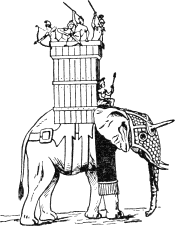
\includegraphics[width=0.3\linewidth]{./graphics/pic37.png}
  \caption{During the early days of typography fonts were designed to emulate the looks of calligraphic texts.}
  \label{fig:marginfig1}
\end{figure}

\section{Inserting figures}

In order to insert figures, the \pkgname{graphicx} package has to included in the preamble (before the |\begin{document}|-command) of your LaTeX-document:

\graybox{\texttt{\textbackslash usepackage\{graphicx\}}}

Originally only EPS-figures could be inserted with the \pkgname{graphic}package. This has now been developed into the  \pkgname{graphicx}, which allows almost any common format to be inserted. 

The simplest way of including a graphic looks like this:


\CMDI{\includegraphics}\marg{filename}


If the image is not located in the same folder as the tex-file, you will have to specify the path relative to the tex-file.

\graybox{\texttt{\textbackslash includegraphics\{./images/filename\}}}


\subsection{Scaling and resizing images}

If you want the image to appear in a different size, you can specifiy the size as a parameter of the |\includegraphics|-command::


\graybox{\texttt{\textbackslash includegraphics[width=3.9cm]\{filename\}}}


This will scale the image to the width of 3.9 centimeters. 

Use |\textwidth| command if you don't want to specify an absolute size but rather want the actual size to depend on the text width of the page. You can use any of the normal \tex units such as \texttt{em, pt, cm, in}:
\graybox{\texttt{\textbackslash includegraphics[width=0.5\textbackslash textwidth]\{filename\}}}
\noindent will scale the image to half of the text width. The images in the
figure below were produced by two |includegraphics| commands. You can have as many as you like and the \tex engine will treat them the same way as text. If you a leave a space between the commands, they will be positioned vertically as they are treated as paragraphs.

\medskip
\begingroup

\centering
\includegraphics[width=0.3\textwidth]{./graphics/amato.jpg}
\includegraphics[width=0.3\textwidth]{./graphics/amato.jpg}
\includegraphics[width=0.3\textwidth]{./graphics/amato.jpg}

\endgroup


The three photos were centered using the |\centering| command, within a group.


\begin{teX}
\begingroup

\centering
\includegraphics[width=0.3\textwidth]{./graphics/amato.jpg}
\includegraphics[width=0.3\textwidth]{./graphics/amato.jpg}
\includegraphics[width=0.3\textwidth]{./graphics/amato.jpg}
\endgroup
\end{teX}

The |\begingroup..\endgroup| is necessary to limit the effect of centering to
the group only, otherwise \tex would center everything from this point onwards.

\subsection{Controlling the aspect ratio}

You can control the picture aspect ratio by using the command:

\CMDI{\includegraphics}[keepaspectratio,width=3cm, height=3cm]]\{filename\}


If set to true then specifying 
both |width| and |height| (or |totalheight|) does not distort the figure but 
scales such that neither of the specified dimensions is exceeded.






\medskip
\begingroup

\centering
\includegraphics[width=0.3\textwidth, height=5cm]{./images/amato.jpg}
\includegraphics[keepaspectratio=true,width=4cm, height=5cm]{./images/amato.jpg}
\includegraphics[width=3cm]{./images/amato.jpg}

\endgroup


This can be very useful if you have images shown side by side with different
aspect ratios. 


\subsection{Paths and file types}

For larger projects you will probably find it more convenient to have 
images in different folders. You can specify default paths using:


\CMDI{\graphicspath}\marg{dir-list}

This optional declaration may be used to specify a list of directories in which to
search for graphics files. The format is the same as for the \latexe primitive
|\input@path|. A list of directories, each in a \{\} group (even if there is only one
in the list). For example:


\graybox{\texttt{\textbackslash graphicspath\{\{eps/\}\{tiff/\}\}}}


The default image formats can be declared using:

\CMDI{\DeclareGraphicsExtensions}\marg{png,jpg}

This specifies the behaviour of the system when no file extension is specified in 
the argument to |\includegraphics|. \texttt{\{ext-list\}} should be a comma separated 
list of file extensions. (White space is ignored between the entries.) A file name
is produced by appending one extension from the list. If a file is found, the
system acts as if that extension had been specified. If not, the next extension
in \texttt{ext-list} is tried.



\subsection{The figure environment}

You use the figure-environment to let your image appear in a "floating" environment, that is \latex will place it at the right position of a page and even on the next page:

\begin{teX}
\begin{figure}
  \includegraphics{filename.eps}
  \caption{title of your figure}
  \label{labelname}
\end{figure}
\end{teX}

Here |\caption{...}| defines the title of the figure which will appear beneath the figure. |\label{..}| defines the label which can be used inside the document in order to insert references to the figure:

The figure

|\ref{labelname} on page \pageref{labelname} ..|

The|\label-command| inside the |\figure|-envirnonment hast to appear just after the|\caption|-command.
placing figures

If figures reside inside a |\figure|-environment, this will cause LaTeX to choose the actual location of the figure inside the document. There are different parameters for the placement strategy:

\begin{description}
\item[h (here)] Try to place the figure just where the command is located.

\item [t (top)] Try to place the figure at the top of the page.

\item[b (bottom)] Try to place the figure at the bottom of the page.

\item [p (float page)] Try to place the figure on a page which contains only floating elements.
\end{description}

The order of these parameters doesn't matter since placement is always tried in the order \textbf{h, t, b, p,} if these parameters are present:

If no parameter is present, the default order is  \texttt{[tbp]}.


The command for a figure-environment might for example look like this:

\begin{teX}
\begin{figure}[htbp]
...
\end{figure}
\end{teX}



\subsection{Table of figures}
\index{figures!Table of figures}
A table of figures is inserted (where you place the command) using the command


\begin{teX}
   \listoffigures
\end{teX}

The caption given in the \cmd{caption} command is also used in the list of figures. 
If you want to use different captions, you may add a parameter to the |\caption| command:
|\caption[caption for listoffigures]{caption inside the document}|


\subsection{Figures with a border}

Although drawing frames around tables should be discouraged, if you find the need
to draw them there are  two possible ways to achieve it: either only the figure itself is bordered or there is a border around the figure and its caption. You place a border around the figure using the \cmd{\fbox} command or the \cmd{\framebox}.

\emphasis{fbox,minipage}
\begin{teX}
\begin{figure}[htbp]
  \centering
  \fbox{
    \includegraphics{filename}
  }
  \caption{caption}
  \label{Labelname}
\end{figure}
\end{teX}

Placing a border around the figure and its title is a little more tricky: You need to place the figure and the title in a |\minipage| environment which is bordered again with the |\fbox| command:

\begin{teX}
\begin{figure}[htbp]
  \centering
  \fbox{
    \begin{minipage}{13 cm}
      \includegraphics{filename}
      \caption{caption}
      \label{labelname}
    \end{minipage}
  }
\end{figure}
\end{teX}

This will produce the image shown below,

\begin{center}
\begin{figure}[htbp]
  \centering
  \fbox{
    \begin{minipage}{0.25\linewidth}
      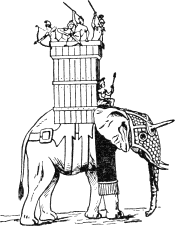
\includegraphics[width=0.9\linewidth]{./graphics/pic37.png}
      \caption{The boxed fighting elephant}
      \label{labelname}
    \end{minipage}
  }
\end{figure}
\end{center}


Unfortunately the width of the border cannot be determined automatically. It has to be specified as a parameter of the |\minipage| environment. However, you may be bale to develop a macro to do this - based on the ImageSize routines we developed in section.


\section{Side by side figures}

You might want to place to figures side by side but to use only one caption. This is achieved by placing both figures in its own |\minipage| which reside in the same |\figure|.

if only one |\caption| command is used, both figures will have a common title:

\medskip
\begin{verbatim}
\begin{figure}[htbp]
  \centering
  \begin{minipage}[b]{5 cm}
    \includegraphics{filename 1}  
  \end{minipage}
  \begin{minipage}[b]{5 cm}
    \includegraphics{filename 2}  
  \end{minipage}
  \caption{common caption}
  \label{Labelname}
\end{figure}
\end{verbatim}
\medskip

The first parameter of the |\minipage| environment determines how both graphics are aligned to each other. b (bottom) aligns the bottom borders of the figures, \textbf{t} (top) aligns the top borders and \textbf{c} aligns the centers.

If you want distinct titles for the two figures you will only have to supply a |\caption| command for both |\minipage|environments:

\begin{teX}
\begin{figure}[htbp]
  \centering
  \begin{minipage}[b]{5 cm}
    \includegraphics{filename 1} 
    \caption{caption 1}
    \label{labelname 1}
  \end{minipage}
  \begin{minipage}[b]{5 cm}
    \includegraphics{filename 2}  
    \caption{caption 2}
    \label{labelname 2}
  \end{minipage}
\end{figure}
\end{teX}


If you want to have subfigures with distinct caption, you use the |\subfig| package:


You can put as many figures as you like on a page, but a word of warning, you may need to make some manual adjustments before you get it right. The package provides support for the manipulation and reference of small or ‘sub’ floats within a single floating (e.g., figure or table) environment1 It is convenient to use this
package when your sub-floats are to be separately captioned, referenced, or when such
sub-captions are to be included on a List-of-Floats page.

The package is a replacement for the subfigure package, from which it was derived.
However, the new subfig package is not completely backward compatible.
Therefore, a new name was called for. The newer package is smaller and easier to use
than the older package, however, it now uses the following additional packages, 
caption (required), 
everysel (optional), 
keyval (required), 
ragged2e (optional).

It will work without the ragged2e and everysel packages if you do not use the following
justification options: ‘Center’, ‘RaggedRight’ and ‘RaggedLeft’. The other justification
options ‘center’, ‘raggedright’ and ‘raggedleft’ will work without the above two packages. If the ragged2e package is present, than the caption package will load it and it
will, in turn, load the everysel package. This happens whether or not you will be using
the justification options that require it. If it cannot find the ragged2e package, than the
caption package will print a message that ‘RaggedRight’, etc. will not be available.



 A low bottle-shaped vase, of yellowish ware, with flaring rim and somewhat flattened body. Height, 5 inches; width 5 inches. \ref{fig:one}

A well-made bottle shaped vase, with low neck and globular body, somewhat conical above. Color dark brownish. 7½ inches in height. Shown in \ref{fig:two}


\begin{figure}
  \centering
  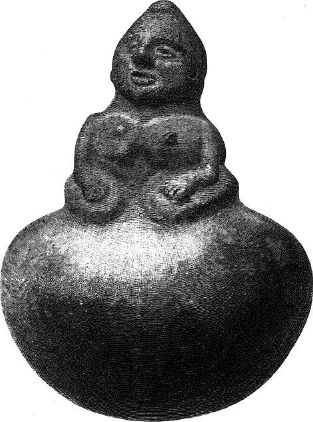
\includegraphics[width=0.7\linewidth]{./graphics/fig175.jpg}
   \centerline{From the tomb of a Pull\= arius.}
  \label{fig:marginfig1}
\end{figure}

The above figure is an effigy vase of the dark ware. The body is globular. A kneeling human figure forms the neck. The mouth of the vessel occurs at the back of the head—a rule in this class of vessels. Is is finely made and symmetrical. 9¾ inches high and 7 inches in diameter. being larger than the above two it is preferable to scale it to give the reader an indication. Based on the figure width, you may also need to adjust the distance between the figures to ensure that the whitespace is just about right. For screen reading this can be increased and for printed works you may wish to make it less.







\section{The wrapfig package}


\captionsetup[wrapfigure]{margin=10pt,font=small,labelfont=bf, name=Fig.} % [wrapfigure]{name=Fig.}


Donald Arseneau has created the \pkg{wrapfig} package to allow people to place figures or
tables at the side of a page and wrap text around them. The package provides the
environments wrapfigure and wraptable. Both environments have two required and
two optional arguments. You can see an example taht uses the package to wrap a picture into such a paragraph of text.

\begin{figure}[82pt]
   \includegraphics[width=\linewidth]{./graphics/cyprus.jpg} 
   \caption{\small Cyprian limestone group of Phoenician dancers, about 6½ in. high. There is a somewhat similar group, also from Cyprus, in the British Museum. The dress, a hooded cowl, appears to be of great antiquity.}
\end{figure}

\begin{wrapfigure}[20]{l}{3.8cm}
\centering\small
\includegraphics[width=\linewidth]{./graphics/egyptdance.jpg}  
\caption{\small The hieroglyphics describe the dance.}
\end{wrapfigure}
Amongst the earliest representations that are comprehensible, we have certain Egyptian paintings, and some of these exhibit postures that evidently had even then a settled meaning, and were a phrase in the sentences of the art. Not only were they settled at such an early period (B.C. 3000, fig. 1) but they appear to have been accepted and handed down to succeeding generations (fig. 2), and what is remarkable in some countries, even to our own times. The accompanying illustrations from Egypt and Greece exhibit what was evidently a traditional attitude. The hand-in-hand dance is another of these.

The earliest accompaniments to dancing appear to have been the clapping of hands, the pipes,[1] the guitar, the tambourine, the castanets, the cymbals, the tambour, and sometimes in the street, the drum.

The following account of Egyptian dancing is from Sir Gardiner Wilkinson's "Ancient Egypt"[2]:—
\begin{figure}
   \includegraphics[width=0.3\linewidth]{./graphics/lotus.jpg} 
   \caption{\small Cyprian limestone group of Phoenician dancers, about 6½ in. high. There is a somewhat similar group, also from Cyprus, in the British Museum. The dress, a hooded cowl, appears to be of great antiquity.}
\end{figure}
"The dance consisted mostly of a succession of figures, in which the performers endeavoured to exhibit a great variety of gesture. Men and women danced at the same time, or in separate parties, but the latter were generally preferred for their superior grace and elegance. Some danced to slow airs, adapted to the style of their movement; the attitudes they assumed frequently partook of a grace not unworthy of the Greeks; and some credit is due to the skill of the artist who represented the subject, which excites additional interest from its being in one of the oldest tombs of Thebes (B.C. 1450, Amenophis II.). Others preferred a lively step, regulated by an appropriate tune; and men sometimes danced with great spirit, bounding from the ground, more in the manner of Europeans than of Eastern people. On these occasions the music was not always composed of many instruments, and here we find only the cylindrical maces and a woman snapping her fingers in the time, in lieu of cymbals or castanets.

\begin{figure}
   \includegraphics[width=0.3\linewidth]{./graphics/patera.jpg} 
   \caption{\small Cyprian limestone group of Phoenician dancers, about 6½ in. high. There is a somewhat similar group, also from Cyprus, in the British Museum. The dress, a hooded cowl, appears to be of great antiquity.}
\end{figure}

"Graceful attitudes and gesticulations were the general style of their dance, but, as in all other countries, the taste of the performance varied according to the rank of the person by whom they were employed, or their own skill, and the dance at the house of a priest differed from that among the uncouth peasantry, etc.

"It was not customary for the upper orders of Egyptians to indulge in this amusement, either in public or private assemblies, and none appear to have practised it but the lower ranks of society, and those who gained their livelihood by attending festive meetings.

"Many of these postures resembled those of the modern ballet, and the pirouette delighted an Egyptian party 3,500 years ago.
\medskip

The wrapped figure is positioned using the \texttt{wrapfigure} environment, as shown below:

\begin{teX}
\begin{wrapfigure}[nlines]{placement}[overhang ]{width }
   \includegraphics[width=3.8cm]{./graphics/egyptdance} 
   \caption{\small The hieroglyphics describe the dance.}
\end{wrapfigure}
\end{teX}

The parameter |nlines|  is the number of narrow lines, and placement is one of r, l, i, o, R, L, I, or
O for right, le, inside, and outside, respectively. The uppercase placement specifiers
differ from their lowercase counterparts in that they force \latex to put the float \emph{here},
whereas the lowercase placement specifiers just give a hint to \latex to place them
\texttt{here}. The \texttt{width} argument is the width of the figure or table that appears in the body
of the environment. Finally, \texttt{overhang} tells LATEX how much the figure should hang out
into the margin of the page. Here is how one may create dangerous paragraphs bends!

The |wrapfig| package is compatible with the |caption| package. You can set the caption parameters using:---

\begin{teX}
\captionsetup[wrapfigure]{<options>}
\end{teX}

If you are probably wondering how |wrapfig| achieves this, you should read the class file. It basically uses |everypar|, and hence the limitations with |\par|. Here is an extract from the class.

\begin{teX}

% Subvert \everypar to float fig and do wrapping.  
% Also for non-float.
\def\WF@startfloating{%
 \WF@everypar\expandafter{\the\everypar}\let\everypar\WF@everypar
 \WF@@everypar{\ifvoid\WF@box\else\WF@floathand\fi \the\everypar
 \WF@wraphand
}}
\end{teX}

Moving now to a more scientific example that the previous ones, we will place two figures
one on top of each other and give them individual, sub-captions as shown in \ref{fig:honey}.
 
\captionsetup[figure]{margin=10pt,font=small,labelfont=bf,format=hang}%

\begin{figure}[htbp]
\centering
  \begin{subfigure}[b]{0.5\textwidth}
  \includegraphics[width=\linewidth]{./graphics/honey.png}
  \caption{Taylor instability in the surface of the honey in an inverted honey jar.}\label{fig:honey}
    \hspace{1cm}
  \end{subfigure}

  \begin{subfigure}[b]{0.9\textwidth}
     \centering
     \includegraphics[width=9cm]{./graphics/honeydrops.png}
     \caption{Taylor instability in the interface of the water condensing on the underside of a small water pipe.}
  \end{subfigure}  
  \caption{Two examples of Taylor instabilities that are commonly found.}%
    \label{fig:Athird}%
\end{figure}

The figures are from A Heat Transfer Textbook, by J.H.Lienhard, which incidentally was typeset using
\tex . It is a McGrawHill publication. 

\begin{teX}
\begin{figure}[htbp]
    \captionsetup[figure]{margin=10pt}%
    \subfloat[Taylor instability...]
     {{\includegraphics[width=8cm]{./graphics/honey}}}
    \hspace{1cm}
     \subfloat[Taylor instability in the...]%
      {\includegraphics[width=9cm]{./graphics/honeydrops}}  
     \\[-10pt]
   \caption{Taylor instability in...}%
    \label{fig:Afirst}%
    \caption{Two examples of... }%
    \label{fig:honey}%
\end{figure}
\end{teX}


The text can have more than one paragraph. It is also possible to include figures
generated by |TikZ/pgf|, as shown in the next example, drawn from real code
in the book.


\begin{wrapfigure}[14]{l}{3.0cm}
\pgfplotsset{width=5.0cm,compat=1.3}
\begin{tikzpicture}
\begin{axis}[minor y tick num=4, 
minor x tick num=4, 
xmin=0,xmax=300,
ymin=0,ymax=60,
xlabel=\textsf{liquidus ($l/s$)},
ylabel=\textsf{capitis ($m$)}, 
ytick={0,15,30,45,60,75},
xtick={0,100,200,300}
]
\addplot[color=blue,mark=x, smooth] coordinates {
(0,44)
(50,43)
(100,42)
(150,40)
(200,33)
(220,29)
};

\end{axis}
\end{tikzpicture}
\caption{Pump headum and flowm}
\end{wrapfigure}


\providecommand\addcredit[1]{%
 \vspace*{-6.5pt}
 \scriptsize%
 \flushright%
 \textit{Credit: #1}%
}
\newpage
\pagestyle{empty}
\thispagestyle{empty}
\begin{figure}[htp]
\centering

\captionsetup{name=Photo., labelsep=period}%
   \begin{minipage}[t]{0.48\textwidth}
      \includegraphics[width=\textwidth]{./graphics/movingup.jpg}%
      \addcredit{U.S. DoD.}%
     \caption{The effects of the credit going past the edge of the figure. This can be corrected by adding a minipage to hold both commands. }
\end{minipage}\hfill\hfill
\begin{minipage}[t]{0.48\textwidth}
      \includegraphics[width=\textwidth]{./graphics/survivors.jpg}%
      \addcredit{U.S. DoD.}%
    {\footnotesize Marines awaiting resting before moving on to Japan. }
\end{minipage}

% \begin{minipage}[t]{0.48\textwidth}
%      \includegraphics[width=\textwidth]{./graphics/img009.jpg}%
%      \addcredit{U.S. DoD.}%
%     \caption{Engineer Construction Troops in Liberia, July 1942.}
%\end{minipage}\hfill\hfill
%\begin{minipage}[t]{0.48\textwidth}
%      \includegraphics[width=\textwidth]{./graphics/survivors.jpg}%
%      \addcredit{U.S. DoD.}%
%     \caption{The effects of the credit going past the edge of the figure. This can be corrected by adding a minipage to hold both commands. }
%\end{minipage}
% \begin{minipage}[t]{0.48\textwidth}
%      \includegraphics[width=\textwidth]{./graphics/img126.jpg}%
%      \addcredit{U.S. DoD.}%
%     \caption{Marine Reinforcements.
%A light machine gun squad of 3d Battalion, 1st Marines, arrives during the battle for ``Boulder City.'' }
%\end{minipage}\hfill\hfill
%\begin{minipage}[t]{0.48\textwidth}
%      \includegraphics[width=\textwidth]{./graphics/img124.jpg}%
%      \addcredit{U.S. DoD.}%
%     \caption{Brothers Under the Skin, inductees at Fort Sam Houston, Texas, 1953. }
%\end{minipage}
\end{figure}
\newpage


Armed with all these packages you can help the Gutenburg organization to transcribe
some of the old books that they have online. 

\clearpage








%  \chapter{WRAPPED ILLUSTRATIONS}
\parindent2em
\let\onepar\lorem

If you are planning to have a more traditional book design wrapped figures are essential. Traditional typographers used
all sorts of styles to achieve this is to use
The best way to achieve it is to use Donald Arseneau's wrafig package.

\begin{wrapfigure}{l}{3.2cm}
    \includegraphics[width=3cm]{amato}
    \caption{\footnotesize Wrapped figures}
\end{wrapfigure}

Get prepared to do a lot of manual adjustments, see your figures disappear on page refreshes and reruns. After a while though you get the hang of it and by minor adjustments you can really achieve great results. The manual uses \verb+everypar+ to insert commands for the shaping of the paragraphs that \emph{follow} the wrapped figure.

Wrapfig.sty provides the environments \pkg{wrapfigure} and \pkg{wraptable} for typesetting a
narrow float at the edge of the text, and making the text wrap around it. The wrapfigure
and wraptable environments interact properly with the \verb+\caption+ command to produce
proper numbering, but they are not regular floats like figure and table, so (beware!)
they may be printed out of sequence with the regular floats. The environment  provides one of those monster commands that stresses one's memory as itprovides for four parameters. 
The four param
for \verb+\begin{wrapfigure}+, two optional and two required, plus the text of the figure, with a caption perhaps.

\begin{macro}{wrapfigure}
\end{macro}

|\begin{wrapfigure}[12]{r}[34pt]{5cm}\meta{figure}\end{wrapfigure}|

  \begin{tikzpicture}[xshift=-15pt]
    \node (number) at (0mm, 0mm) {\oarg{number of narrow lines}};
    \node (placement) at (36mm, 0mm) {\marg{placement}};
    \node (overhang) at (60mm, 0mm) {\oarg{overhang}};
    \node (width) at (81mm, 0mm) {\marg{width}};
    \begin{scope}[->]
    \draw (number) -- (16mm, 17mm);
    \draw (placement) -- (24mm, 17mm);
    \draw (overhang) -- (35mm, 17mm);
    \draw (width) -- (47mm, 17mm);
    \end{scope}
  \end{tikzpicture}


First we will look at placing the figure without the use of optional commands.


\begin{verbatim}
\begin{wrapfigure}{r}{.4\textwidth}
    \includegraphics[width=.4\textwidth]{./path/file}
    \caption{\footnotesize Wrapped figures}
\end{wrapfigure}
\end{verbatim}

From the four parameters the first one indicates if the figure is to be typeset left or right.

\begin{verbatim}
\begin{wrapfigure}{l}{\imagewidth}
    \includegraphics[width=\imagewidth



]{./graphics/parasol-01}
    \caption{\footnotesize Wrapped figures}
\end{wrapfigure}
\end{verbatim}


\begin{wrapfigure}[16]{I}[0.1pt]{85pt}
    \vskip-10.5pt plus 2pt minus 2pt\relax
    \includegraphics[width=83pt]{parasol-01}
    \caption{\scriptsize Wrapped figures, parameters set at \texttt\{l\}\{90pt\}.}
\end{wrapfigure}

Changing the parameters to suit we now have the illustration floating to the left. Allowing for the figure to be approximately two point  wider than the actual graphic, will leave a bit more margin. If the figure is end low in the page you need to be careful, that it does not disappear, as you will not get any warning.

The first parameter we are going to use an optional parameter is the one that determines the number of narrow lines. The format is \verb+[narrowlines]{l}{90pt}+. Think of this parameter as a fine tuning parameter and do not touch it until after your final draft is ready. If you see indented lines at the beginning of the page that follows the wrapped figure, reduce the number of lines, until you get satisfactory results.

The second optional parameter, comes after the \texttt{\{r\}[overhang]} parameter.

The second optional parameter (\#3) tells how much the figure should hang out into
the margin. The default overhang is given by the length \verb+\wrapoverhang+, which is 0pt
normally but can be changed using |\setlength|. For example, to have all wrapfigures
use the space reserved for marginal notes,

\begin{verbatim}
\setlength{\wrapoverhang}{\marginparwidth}
\addtolength{\wrapoverhang}{\marginparsep}
\end{verbatim}

Again not recommended. The best approach is to specify the figures with O or I, let them float and if the results are
not very good then make manual adjustments. Get prepared to spend at least 5-10 minutes fiddling with the final result.

When you do specify the overhang explicitly for a particular figure, you can use a
special unit called \string\width meaning the width of the figure. For example, [0.5\string\width]
makes the center of the figure sit on the edge of the text, and [\string\width] puts the figure
entirely in the margin (and the adjacent text is indented by just \string\columnsep). This
\texttt{\string\width} is the actual width of the wrapfigure, which may be greater than the declared
width.

\begin{figure}[tb]
\includegraphics[width=\textwidth]{chiefs}
\caption{Chiefs of Kelau or Kelaou.}
\label{fig:chiefs}
\end{figure}

\begin{figure}[p]
\centering

\includegraphics[width=0.8\textwidth,height=0.9\textheight, keepaspectratio]{parasol-01}
\caption{Chiefs of Kelau or Kelaou.}
\label{fig:parasol-01}
\end{figure}

\section{Balancing the illustrations}

Illustrations come in various sizes, but in general they need to flow with the text. Place figures on top of the page and figures that would dominate the text on their own page. For example Figure~\ref{fig:chiefs} was allowed to float to the top of a page whereas Figure~\ref{fig:parasol-01} was placed on its own page, as I thought it will overwhelm the text if shown in a large size. However the same figure seems perfectly alright as a wrapped figure.

\begin{texexample}{}{}
\begin{wrapfigure}{I}{0pt}
    \includegraphics[width=75pt]{parasol-01}
 \end{wrapfigure}
\lipsum[1-2]
\begin{wrapfigure}{l}{0pt}
    \includegraphics[width=75pt]{parasol-01}
 \end{wrapfigure}
\lipsum[1-2]
\end{texexample}



\begin{texexample}{}{}
\begin{wrapfigure}{l}{0pt}
    \includegraphics[width=70pt]{parasol-01}
    \includegraphics[width=70pt]{parasol-01}
 \end{wrapfigure}

\lipsum[1-3]\lorem
\end{texexample}




\begin{texexample}{}{}
\begin{wrapfigure}[13]{L}{0pt}
    \includegraphics[width=100pt]{conicalbasket}
\end{wrapfigure}

\onepar\onepar\onepar

\end{texexample}




%  \makeatletter
\newcommand\QEDit{\hspace{6pt}\textit{Q.~E.~D.}\quad}
\newcommand\QEFit{\hspace{6pt}\textit{Q.~E.~F.}\quad}
\newcommand\QEIit{\hspace{6pt}\textit{Q.~E.~I.}\quad}
\newcommand\QEDup{\hspace{6pt}Q.~E.~D.\quad}
\newcommand\QEFup{\hspace{6pt}Q.~E.~F.\quad}
\newcommand\QEIup{\hspace{6pt}Q.~E.~I.\quad}
\newcommand\QEOup{\hspace{6pt}Q.~E.~O.\quad}
\newcounter{wrapwidth}
\newcount \Zw
\newcount \Zh


\newcommand\pngright[4]{%
    \Zw=#2 \divide \Zw by 10
    \Zh=#3 \divide \Zh by 120  \advance\Zh by 1
    \setcounter{wrapwidth}{\Zw}
\begin{wrapfigure}[\Zh]{r}{\value{wrapwidth}pt}%
\begin{center}
\vspace{#4pt}%
\includegraphics*[width=\Zw pt]{images/#1}%
\end{center}
\end{wrapfigure}}

\newcommand\propnopage[1]{
\begin{center}{\large #1}\end{center}}

\parindent1em

\cxset{toc image=\@empty}
\chapter{PERICULA}

\noindent\textsc{Case Study: } We will now typeset a section, from Isaac Newton's \textit{Philosophi\ae\  Naturalis Principia Mathematica}. The typeset example is shown below.

\bottomline
\bgroup
\small

\cxset{section align=center,
         section numbering=none}

\section{{SECT}$\cdot$ VIII$\cdot$}

\begin{center}{\textit{De Motu per Fluida propagato.}}\end{center}

\makeatletter
%\propnopage{Prop.\ XLI\@. Theor.\ XXXI.}
\meaning\@
\makeatother

\textit{Pressio non propagatur per Fluidum secundum lineas rectas, nisi
ubi particul{\ae} Fluidi in directum jacent.}

Si jaceant particul{\ae} $a$, $b$, $c$, $d$, $e$ in linea recta, potest quidem
pressio directe

\begin{wrapfigure}[8]{O}[1pt]{0.3\textwidth}
  \vspace{-17pt}
  \includegraphics[width=0.27\textwidth]{images/362.png}
\end{wrapfigure}

\noindent propagari  ab $a$ ad $e$; at
particula $e$ urgebit particulas oblique positas
$f$ \& $g$ oblique, \& particul{\ae} ill{\ae} $f$ \& $g$
non sustinebunt pressionem illatam, nisi fulciantur
a particulis ulterioribus $h$ \& $k$;
quatenus autem fulciuntur, premunt particulas
fulcientes; \& h{\ae} non sustinebunt pressionem nisi fulciantur
ab ulterioribus $l$ \& $m$ easque premant, \& sic deinceps in infinitum.
Pressio igitur, quam primum propagatur ad particulas
qu{\ae} non in directum jacent, divaricare incipiet \& oblique propagabitur
in infinitum; \& postquam incipit oblique propagari, si
inciderit in particulas ulteriores, qu{\ae} non in directum jacent, iterum
divaricabit; idque toties, quoties in particulas non accurate
in directum jacentes inciderit. \QEDit

\topline

\vspace*{-\baselineskip}
\captionof{figure}{Example of a typeset page from Principi\ae.}
\egroup
\smallskip
Figure~\ref{fig:principia}, shows a scan of the actual page. We will not reproduce, the fonts and the page geometry exactly, but rather we will attempt to extract and reproduce the typographical rules employed in the printing of the \textit{Principi\ae}.

We begin by typesetting the section number and its heading. The use of roman numbers creates better harmony between the text and the heading

\begin{teX}
\sectpage{VIII$\middot$}
\begin{center}{\textit{De Motu per Fluida propagato.}}\end{center}
\end{teX}
The proposition and theorem line, has its own command
\begin{teX}
\makeatletter
\propnopage{Prop.\ XLI. Theor.\ XXXI.}
\makeatother
\end{teX}

\propnopage{\color{gray}Prop.\ XLI\@. Theor.\ XXXI.}
\vspace*{-37pt}
\propnopage{Prop. XLI. Theor. XXXI.}


Notice the small differences in the spacing with the commands as shown and with the black text, without them. The rest is based on normal \LaTeX\ commands.

\textit{Pressio non propagatur \ldots particul{\ae}\ldots}

\pngright{362.png}{709}{603}{-24}

Si jaceant particul{\ae} $a$, $b$, $c$, $d$,
$e$ in linea recta, potest quidem
pressio directe propagari ab $a$ ad $e$; at


Remember that it is important to start a new paragraph after the 
|pngright| command. The |wrapfig| package works by using |everypar| to insert the hanging indentation.

\begin{figure}[p]
\centering
\includegraphics[scale=1]{./images/page354.png}
\caption{Page 354 from Isaac Newton's \textit{Philosophi\ae\  Naturalis Principia Mathematica}. Image was obtained from Google's copy, available at Google Books.}
\label{fig:principia}
\end{figure}
\makeatother

%  \chapter{Subfigures}

So far we have been using the |caption| package to add captions to multiple figures, that are numbered individually, but how about if you want to have only one caption and number the subfigures alphabetically. If you want to have |subfigures| with distinct caption, you use the |subfig| package \citep{subfigure}. A newer package \ctan{subcaption} is also now available with the |caption| suite and we will discuss this also. The two packages are incompatible and the recommendation is to use the |subcaption| package. In the |phd| class we load the |caption| package which also loads the |subcaption| package. The latter is to be preferred as it integrates better both with captions as well as the |hyperref| package.

\begin{figure}[h]
\centering
\begin{minipage}[b]{.3\linewidth}
\includegraphics[width=4cm]{./graphics/pic37.png}\hspace{1em}
\subcaption{First fighting elephant}\label{fig:1a}
\end{minipage}\hspace{1em}
\begin{minipage}[b]{.3\linewidth}
\includegraphics[width=4cm]{./graphics/pic37.png}\hspace{1em}
\subcaption{Second fighting  elephant}\label{fig:1b}
\end{minipage}\hspace{1em}
\begin{minipage}[b]{.3\linewidth}
\includegraphics[width=4cm]{./graphics/pic37.png}\hspace{1em}
\subcaption{Third fighting elephant}\label{fig:1c}
\end{minipage}
\caption{Three fighting elephants example}
\end{figure}

You can put as many figures as you like on a page, but a word of warning, you may need to make some manual adjustments before you get it right. The package provides support for the manipulation and reference of small or \enquote{sub} floats within a single floating (e.g., figure or table) environment It is convenient to use this
package when your sub-floats are to be separately captioned, referenced, or when such
sub-captions are to be included on a List of Floats page.

The package is a replacement for the |subfigure| package, from which it was derived.
However, the new |subfig| package is not completely backward compatible.
Therefore, a new name was called for. The newer package is smaller and easier to use
than the older package, however, it now uses the following additional packages,  |caption| (required),  |everysel| (optional),
keyval (required),  |ragged2e| (optional). All these packages are included with the |phd| auto package manager.

It will work without the |ragged2e| and |everysel| packages if you do not use the following
justification options: \enquote{Center}, \enquote{RaggedRight} and \enquote{RaggedLeft}. The other justification
options \enquote{center}, \enquote{raggedright} and \enquote{raggedleft} will work without the above two packages. If the ragged2e package is present, than the caption package will load it and it
will, in turn, load the everysel package. This happens whether or not you will be using
the justification options that require it. If it cannot find the ragged2e package, than the
caption package will print a message that \enquote{RaggedRight}, etc. will not be available.

\section{Subcaption environments}

The |subcaption| package offers an environment for subfigures, which are essentially minipages. Within the environment, the normal caption command can be used rather than the \cmd{\subcaption}.

\begin{figure}%
    \centering
    \captionsetup[figure]{margin=3pt}%
    \begin{subfigure}[b]{.35\linewidth}
    \includegraphics[scale=0.65]{./graphics/fig155.jpg} 
    \label{fig:one}
    \caption{First Caption}
    \end{subfigure}\hspace{2em}
    \begin{subfigure}[b]{.35\linewidth}
    \includegraphics[scale=0.65]{./graphics/fig156.jpg} 
    \caption{First Caption}
    \end{subfigure}
    \caption{Two subfigures side by side.}
    \label{fig:two}
\end{figure}

The sub-figures can be referenced the same way as normal referencing.

\begin{quote}
 A low bottle-shaped vase, of yellowish ware, with flaring rim and somewhat flattened body. Height, 5 inches; width 5 inches. \ref{fig:one}


A well-made bottle shaped vase, with low neck and globular body, somewhat conical above. Color dark brownish. $7\frac{1}{2}$ inches in height. Shown in Figure~\ref{fig:two}.
\end{quote}

\begin{figure}[htp]
  \centering
  \includegraphics[width=0.5\linewidth]{./graphics/fig175.jpg}
  \vspace{3\baselineskip}

   \centerline{\textsc{From the tomb of a Pull\= arius.}}
  \label{fig:marginfig1}
  \caption{ effigy vase of the dark ware. The body is globular. A kneeling human figure forms the neck. The mouth of the vessel occurs at the back of the head—a rule in this class of vessels. Is is finely made and symmetrical. 9.75 inches high and 7 inches in diameter. being larger than the above two it is preferable to scale it to give the reader an indication.}
\end{figure}

The above figure is an Based on the figure width, you may also need to adjust the distance between the figures to ensure that the whitespace is just about right. For screen reading this can be increased and for printed works you may wish to make it less.

\begin{teXXX}
\begin{figure}[htb]
\begin{subfigure}[b]{.5\linewidth}
\centering\large A
\captionsetup{skip=3pt}
\caption{A subfigure}\label{fig:1a}
\end{subfigure}
\end{figure}
\end{teXXX}

\begin{comment}
\begin{figure}[htp]%
    \captionsetup[figure]{margin=3pt}%
    \subfloat[One subone.\label{fig:one}]
     {{\includegraphics[scale=0.65]{./graphics/fig155.jpg}}}
    \hspace{1cm}
    \subfloat[One subtwo.\label{fig:two} --- but this one has a
     very very long caption.  So long that it continues over into
     other lines so that we can test the list-of line settings.]%
      {\includegraphics[scale=0.65]{./graphics/fig156.jpg}}
     \\[-10pt]
    \caption{First figure --- but this one has a very very long caption.
     So long that it continues over into a second line so that we can
     test the margin setting and centering of the caption command in the
     full page mode.}%
    \label{fig:Afirst}%
    \caption{Typical pottery from Oklahoma (\emph{Smithsonian}).}%
    \label{fig:Athird}%
\end{figure}
\end{comment}

The figures have been placed using the code below:

\begin{verbatim}
\begin{figure}%
    \captionsetup[figure]{margin=3pt}%
    \subfloat[One subone.\label{fig:one}]
     {{\includegraphics[scale=0.65]{./graphics/fig155.jpg}}}
    \hspace{1cm}
    \subfloat[One subtwo.\label{fig:two} --- but this one has a
     very very long caption.  So long that it continues over into
     other lines so that we can test the list-of line settings.]%
      {\includegraphics[scale=0.65]{./graphics/fig156.jpg}}
     \\[-10pt]
 \caption{First figure but this one has a very very long caption.
 So long that it continues over into a second line so that we can
 test the margin setting and centering of the caption command in the
 full page mode.}%
 \label{fig:Afirst}%
 \caption{Typical pottery from Oklahoma (\emph{Smithsonian}).}%
 \label{fig:Athird}%
\end{figure}
\end{verbatim}

As you can observe, the |subcaption| package treats the two figures as one and places them side by side. Its trickery is to get them to line up, nicely and to provide all the necessary parameters for the captions. It is a feature-rich package and we will spent some time to explore it. The command |subfloat|, is used to denote the |subfigure|. The rest are self-explanatory. Note that the use of |\hspace{1cm}| to make these two figures come closer together. In the previous listings, |\hfill| was used to space them out as wide as possible. The command |captionsetup| is used to let the package know that we are captioning figures and not tables. (In this book all captions are placed in the side-margins, where God meant them to be! If you use the same code in another package they will be placed underneath the figures.




%  \begin{comment}
\documentclass[imperial, justified]{octavo}
\usepackage{caption}
\usepackage{natbib}
\usepackage{lstdoc}
\usepackage{lipsum}
\usepackage{graphicx}
\usepackage{overpic}
\usepackage{url}
\global\setlength\parindent{1em}
\newif\ifdebug
\debugfalse
\ifdebug  
  \setlength\fboxsep{1pt}
\else
  \setlength\fboxsep{0pt}
  \setlength\fboxrule{0pt}
\fi

%% temporary titles
% command to provide stretchy vertical space in proportion
\newcommand\nbvspace[1][1]{\vspace*{\stretch{#1}}}

% allow some slack to avoid under/overfull boxes
\newcommand\nbstretchyspace{\spaceskip0.5em plus 0.25em minus 0.25em}

% To improve spacing on titlepages
\newcommand{\nbtitlestretch}{\spaceskip0.6em}

% temporary length used for some tables
\newlength{\TmpLen}

\begin{document}
\clearpage
\pagestyle{empty}
\begin{center}
\bfseries

\nbvspace[1]
\Huge
{\nbtitlestretch\huge
 TYPESETTING  
WITH  \TeX\ AND SX.TX FRIENDS  \\
}

\nbvspace[2]
\normalsize
TO WHICH IS ADDED MANY USEFUL MACROS
AND CODE WRITTEN SO THAT HE WHO RUNS MAY HACK

\nbvspace[1]
\small BY\\
\nbvspace[1]
\Large THE STACKEXCHANGE COMMUNITY {\large\textsc{}}\\[0.5em]
%\footnotesize AUTHOR OF ``A WORKING ALGEBRA,'' ``WIRELESS TELEGRAPHY,\\
%ITS HISTORY, THEORY AND PRACTICE,'' ETC., ETC.

\nbvspace[4]

%\includegraphics[width=0.8in]{ejc.pdf}
\includegraphics[width=1.5in]{./images/fig176}
\par
\nbvspace[2]
\normalsize
%DOHA$\cdot$BERLIN$ \cdot$ WILD

\nbvspace[10]
\Large
PUBLISHED IN THE WILD
%
\end{center}


\long\def\secondpage{\clearpage\null\vfill\vfill
\pagestyle{empty}
\begin{minipage}[b]{0.9\textwidth}
\footnotesize\raggedright
\setlength{\parskip}{0.5\baselineskip}
Copyright \copyright 2010--\the\year\ Dr Yiannis Lazarides\par
Permission is granted to copy, distribute and\slash or modify this document under the terms of the GNU Free Documentation License, version 1.2, with no invariant sections, no front-cover texts, and no back-cover texts.\par
A copy of the license is included in the appendix.\par
This document is distributed in the hope that it will be useful, but without any warranty; without even the implied warranty of merchantability or fitness for a particular purpose.
\end{minipage}
\vspace*{2\baselineskip}}

\secondpage

\backmatter
\tableofcontents
\listoffigures

\chapter{PREFACE}
This small booklet aims to describe some of the common problems encountered with the 
placement of figures in books. It also tries to provide techniques for storing them within TeX.

\mainmatter
\end{comment}

\chapter{How to Typeset a lot of Figures}
\label{ch:longfigures}

\precis{In this chapter we develop a primitive database for storing graphics and then typesetting them.}
\addtocimage{-12pt}{-20pt}{../images/tocblock-men.jpg}


If you have a lot of figures, it is a lot of work to have to maintain them, as well as
to remember all the file names. The figures are from an old Catalogue of the Smithsonian Institution \citep{holmes1884}. 

\section{A long table for figures}

We are familiar with longtable for tables, this is an equivalent technique for lots of figures.
\smallskip

\def\figurename{\textbf{Plate}}

\DeclareRobustCommand\putgraphic[1]{%
\fboxsep0pt\fboxrule0pt
\fbox{%
\begin{minipage}[b]{2.0cm}%
 \centering
 \vspace{3.8pt}\fbox{%
 \includegraphics[width=0.98\linewidth,
                 height=2.3cm,
                 keepaspectratio]{./images-01/#1.jpg}}%
  \vspace{0.2cm} #1%
  \vspace{0.2cm}%
  \end{minipage}}\hfil
}

\long\def\putcaption#1{\captionof{figure}{#1}}

\makeatletter
{\centering

\gdef\alist{fig145,fig161,fig162,fig163,fig164,fig165,fig166,fig167,^^A,
fig168,fig169,fig170,fig171,fig172,fig173,^^A
fig174,fig175,fig176,fig177,fig180,fig181,fig182,fig183,fig185,fig186,fig187,fig188,fig189}
\@for \i:=\alist\do{^^A
\expandafter\putgraphic{\i}
}
\putcaption{Weaving and pottery artifacts from Arizona.}}

\medskip

The code leverages \tex's ability to create macro names with any character using the |\csname...\endcsname| construct. We first put the
images in a list. The images have been saved as |fig145| etc on the disk and hence what we simply do is just enclose them in a comma delimited list. They do not need to be numbered consequentially in the list.

\begin{verbatim}
\gdef\alist{fig145,fig161,fig162,..,fig187,fig188,fig189}
\end{verbatim}

We then loop over the |\alist| and get the output as shown in Example~\ref{ex:blist}. 

\begin{texexample}{Looping over the list}{ex:blist}
\def\blist{fig189,fig145,fig161,fig162}
\@for \i:=\blist\do{%
  \expandafter\putgraphic{\i}%
}
\end{texexample}


\section{More on figures and looping}

We can extend our macros and try and save some information for each image. To do this we
need to have a way to associate information with the figure number so we will create a number of commands
for each figure.

The \TeX\ way of defining commands on the fly that include non-letters is to use \verb+\csname+
\begin{verbatim}
\expandafter\def\csname fig170\endcsname#1{#1}
\@nameuse{fig170}{Pottery found in Apache%
    lands in Texas.}
\end{verbatim}

\@nameuse{fig170}{Pottery found in Apache %
    lands in Texas.}

This is not very useful, as it is. It is preferable to actually create a little command factory, that can create these
commands.

\begin{texexample}{}{factory command}
\bgroup
\gdef\commandfactory#1#2{
   \expandafter\def\csname #1\endcsname{#1}
   \expandafter\def\csname #1@caption\endcsname{#2}
}
\commandfactory{fig170}{Test}
\centering

\putgraphic{\csname fig170\endcsname}
\putcaption{\@nameuse{fig170@caption}}

\egroup
\end{texexample}

Since we are going to have to type a lot of information into a database to hold information for our images, we might as
well type it straight into our text.

Out of consideration for our users we may want to provide a short command for this.

\begin{verbatim}
\let\img\commandfactory
\end{verbatim}

\let\img\commandfactory

\img{fig171}{Testing again for something.}

We may also want to save the use of the curly brackets, that would visually distruct. We can redefine the Command factory to be a delimited macro. There is a lot of information on delimited macros. One of them is in such a place, hiding on \texttt{tex.sx}.

\def\commandfactory#1|#2|{
   \expandafter\def\csname #1\endcsname{#1}
   \expandafter\def\csname #1@caption\endcsname{#2}
}

\commandfactory fig172|This is figure 172|

\commandfactory fig173|This is figure 173|

\texttt{\@nameuse{fig172@caption}}

\texttt{\@nameuse{fig173@caption}}

Now that we have figured a way to define an efficient way to store information for our figures, we need to build some routines to sort them print them and other similar housekeeping routines.

\section{Sorting}

\global\setlength\parindent{1em}
I have still to find a better sorting routine other than the one available in the listings documentation. I did try my hands with LuaTeX but I am not very fond of jumping in and out of LaTeX. It can also create problems with updates and users that might not have LuaTeX installed.

We will store the record index in a macro that is essentially a comma delimited list. Don't be frighten about speed
I have used this method to store over 4000 figures and there was no problem either with the processing speed or with TeX'es memory.

We call this macro \verb+dbartifacts+, giving it a non-generic name. But first let us see, how we can add items in
and out of the macro. We start from an empty macro.

\begin{verbatim}
\def\dbartifacts{ }
\end{verbatim}
\let\dbartifacts\empty

We can use \LaTeX's \verb+\g@addto@macro+ to then add the items to the \verb+\dbartifacts+ macro.
\begin{verbatim}
\g@addto@macro{\dbartifacts}{fig172,}%
\g@addto@macro{\dbartifacts}{fig173,}%
\end{verbatim}

\g@addto@macro{\dbartifacts}{fig172,}%
\g@addto@macro{\dbartifacts}{fig173,}%


Testing it by just typing \verb+\texttt{\dbartifacts}+ we get: \texttt{\dbartifacts}. This of course is not very convenient and we would rather define a macro to save all the typing and have a more user friendly command.

\begin{verbatim}
\def\addtodb#1#2{%
  \g@addto@macro#1{#2,}%
}
\end{verbatim}
\def\addtodb#1#2{%
  \g@addto@macro#1{#2,}%
  \lst@BubbleSort\dbartifacts%
}

\clearpage

There are many other ways to manipulate the list, including using token registers, elt lists etc, but for such constructions as the ones described here, this is by far the simpler and the easiest.
We can now use this macro, when required:

\begin{verbatim}
\addtodb{\dbartifacts}{fig170}%
\addtodb{\dbartifacts}{fig171}%
\end{verbatim}

Testing again we get \texttt{\dbartifacts} an as you can see it works nicely. This method of trying out your code bit by bit, I call the water painting technique. So now that we have almost got all the routines we want, we can now look at sorting. This we achieve by adding \verb+ \lst@BubbleSort\dbartifacts+. Every time we add a record, the file will be sorted. Intuituitevely, this might not  be very efficient, especially if you are adding a lot of records at one time, but we can add more helper routines later for this.

\begin{verbatim}
\def\addtodb#1#2{%
  \g@addto@macro#1{#2,}%
  \lst@BubbleSort\dbartifacts%
}
\end{verbatim}

\def\figurename{\textbf{Figure}}
\begin{figure}
\vspace*{1cm}
\centering
\includegraphics[scale=0.6]{./images/fig172.jpg}
\caption{Textiles from Arizona. }
\end{figure}

\section{Adding some more user helper macros}

It is expected that the user will produce a file, either through some automatic means or by typing it to hold the data. Deletion and insertion is simply via editing this file through a text editor. However, for completeness, we will write a few macros to help with maintenace of the database. These include macros for delete and modify record etc.

Another set of macros that one can use is to typet the records in lists and or tabulat forms, if required. Early books on archaelogy for example listed all the items in the following format, interspersed with comments and figures.
\smallskip


\hangindent3em
2520. (39510). A double globe jar or canteen. White ground, with ornamentations in black, as seen in Fig. 649. Depression in the center is probably designed to receive a band or cord to carry it with.
\smallskip

Although one is tempted to produce a list for these, the next item from such a book points otherwise:
\smallskip

\hangindent3em
2677-2678. 2677, (39617), and 2678, (39618). With flared and notched rim.
\smallskip

Before extending the database for such forms of descriptions, we can develop the typesetting part. I am sure that Lamport would have used a list, possibly due memory and space limitations and just re-use the \verb+\item+ command, in our case it is better to rather define a small macro
to cater for such items. The indentation can easily be achieved using \verb+\hangindent3em+ or a similar amount of measure.

\begin{verbatim}
\long\def\catno#1\par{
\par%
\hangindent3em\noindent
#1
}
\end{verbatim}


\def\catno#1#2{%
    \@hangfrom{#1. }#2
}


\DescribeMacro{\@hangfrom}\marg{text}   
\LaTeX\ provides a macro named \verb+\@hangfrom{<text>}+, that puts \marg{text} in a box, and makes a hanging indentation of the following material up to the first \verb+\par+. This Should be used in vertical mode.\footnote{See source2e, \texttt{ltsect.dtx}, pg 287.}

\begin{verbatim}
121 \def\@hangfrom#1{\setbox\@tempboxa\hbox{{#1}}%
122 \hangindent \wd\@tempboxa\noindent\box\@tempboxa}
\end{verbatim}

\medskip

\catno{289}{(39914). Fig. 397. Red ware, with white lines on the lower globe and decorations in black on the upper, with orifice in each globe.}

\catno{1289}{(39914). Fig. 397. Red ware, with white lines on the lower globe and decorations in black on the upper, with orifice in each globe.}


\makeatother

\section{Epiloque}

We have managed to write a database, sort it, typeset its contents in a structured or freeform manner
and on the way we have documented the code using a form of \textit{literate programing.} On top which
other language expects you to code your own ifs and for? 
The amount of code we wrote was very minimal and competes well with modern computer languages. 

Hope you had fun. Go and make beautiful books. 

\begin{figure}[htp]
\centering
{\color{thegray}
\fbox{\includegraphics[width=1\linewidth]{./images//pottery-figures.pdf}}}
\caption{Many books in the humanities have figure pages, with many different styles and numbering schemes. This page extract is from \textit{The Cypro-Phoenician pottery of the Iron Age. }  \protect\cite{schreiber1971} }
\end{figure}


\begin{figure}[htp]
\centering
{\color{thegray}
\fbox{\includegraphics[width=1\linewidth]{./images/sample-tof.pdf}}}
\caption{Many books in the humanities have figure pages, with many different styles and numbering schemes. This page extract is from \textit{The Cypro-Phoenician pottery of the Iron Age. }  \cite{schreiber1971} and shows a specific way of numbering subfigures, including references.}
\end{figure}
\clearpage



 \subsection{Acknowledgements}

 Octavo is a modification of \texttt{classes.dtx} written by Leslie Lamport (1992),
 Frank Mittelbach (1994-97) and Johannes Braams (1994-97). As can be seen
 from the code, my own input is restricted to a tweaking of some parameters
 and true credit is due to Lamport, Mittelbach and Braams for their
 monumental efforts.



\begin{comment}
 \begin{thebibliography}{16}

 \bibitem{knuth98} Knuth,~D. 1998. \emph{Digital Typography}. CSLI 
 Publications, Stanford.

 \bibitem{rosarivo61} Rosarivo,~R. 1961. \emph{Divina proportio typographica}. 
 Scherpe, Krefeld.

 \bibitem{taylor98} Taylor,~P. 1998. \emph{Book design for \TeX\ users, Part 1: 
 Theory.} TUGBoat, 19:65--74.

 \bibitem{taylor99} Taylor,~P. 1999. \emph{Book design for \TeX\ users, Part 2:
 Practice.} TUGBoat, 20:378--389.

 \bibitem{town} Town,~L. \emph{Bookbinding by hand.} Faber \& Faber, London.

 \bibitem{tschichold87} Tschichold,~ J. 1987. \emph{Ausgew\"{a}hlte Aufs\"{a}tze
 \"{u}ber Fragen der Gestalt des Buches und der Typographie}. Birkh\"{a}user
 Verlag, Basel.

 \bibitem{williamson66} Williamson,~H. 1966. \emph{Methods of book design.} Oxford 
 University Press, Oxford.

 \bibitem{wilson01} Wilson,~P. 2001. \emph{The Memoir class for configurable
 typesetting.} CTAN. \url{macros\\latex\\contrib\\memoir} 

 \end{thebibliography}
\end{comment}





\chapter[Overflowing Figures into Margins]{OVERFLOWING FIGURES INTO MARGINS}

Most users of \TeX\ are accustomed to let the system position images, either on top or bottom of the page and occasionally use the [h] positioning directive to place the image at the exact location it appears in the text. Traditional typography placed the image in many different positions. It also occasionally overflowed the image into the margins. The image below, copied from the \textit{American Antiquarian}, was placed in the original publication as such. Tufte advocates the use of such techniques in displaying not only information, but also other material such as tables. The Tufte class is discussed extensively in other sections. It has almost a religious following attached to it and I have personally used it for business reports. \citep{seraphini}

\begin{figure}[htbp]
\leftskip-.07\textwidth\includegraphics[width=1.14\textwidth]{./images/elephant-long.jpg}\par

\begin{center}
\ifdefined\myanmar

လူတိုင်းသည် တူညီ လွတ်လပ်သော ဂုဏ်သိက္ခါဖြင့် လည်းကောင်း၊ တူညီလွတ်လပ်သော အခွင့်အရေးများဖြင့် လည်းကောင်း၊ မွေးဖွားလာသူများ ဖြစ်သည်။ ထိုသူတို့၌ ပိုင်းခြား ဝေဖန်တတ်သော ဉာဏ်နှင့် ကျင့်ဝတ် သိတတ်သော စိတ်တို့ရှိကြ၍ ထိုသူတို့သည် အချင်းချင်း မေတ္တာထား၍ ဆက်ဆံကျင့်သုံးသင့်၏။
\fi
\protect\textsc{Codex Seraphinianus, Mystery Procession \protect\citep{seraphini}}.
\end{center}
\end{figure}

Almost as a matter of rule, the caption for these images was in small caps. Using small caps brought the caption into the easy attention of the reader, but it did not distract from the other elements of the page.
The image is not necessarily positioned symmetrically in the page, you can offset it to suit your taste, but in general, unless the image has any particular features that would make it look better offset rather than centered, is best positioned symmetrically. This can be automated, by writing a macro that measures the dimensions of the image and introduces a \verb+\leftskip+ so that the image can be shifted accordingly. A macro to achieve this is now described.


The first thing we need to do is to increase the \cmd{\textwidth} of the figure to and then to pull it back into
the margin by half the amount. In the example below we use a \cmd{\leftskip-.07} and a \texttt{[width=1.14\string\textwidth]} to set the image width. If we had a lot of similar figures we could create a macro to do this automatically.

\begin{teX}
\begin{figure}[htbp]
\leftskip-.07%
   \textwidth\includegraphics[width=1.14\textwidth]{imagefile}\par
\end{figure}
\end{teX}

If you curious about the script in the caption of the figure it was typeset using a Myanmar script font, which I found it was as mysterious to me, as the script used in \textit{Codex Serafinianus}. 


\long\def\imghangleft#1#2{%
     \figure
     \leftskip-#2\textwidth\includegraphics[width=#1\textwidth]{./images/elephant-long.jpg}\par
     \centerline{\textsc{Codex Serafinianus}}
    \endfigure
}

\imghangleft{1.14}{.07}






%  \section{Sideways Figures}

In my opinion it is bad typography to force one to turn either one's head or turn the book to view an image or to read text. Nevertheless there are exceptions to the rules and hence try and avoid it, as far as possible. A rotating figure or table, must have its caption at the outer edge of the book and hence the image needs to be rotated in the right direction, depending if the page is \textit{verso} or \textit{recto}.
 
Figures can be rotated as shown in Figure~\ref{fig:sideways}  a landscape mode using the \texttt{rotating} package.\index{rotating>sideways package} A package for rotated objects in \latex2e developed by
Robin Fairbairns, Sebastian Rahtz, Leonor Barroca.

\begin{environment}{sideways}
The code uses the |sideways| environment. In this particular example, we use footnotes, in the caption and hence we add some code to achieve this.  Note that the package defaults take care of \textit{verso} and \textit{recto} page display so that you do not need to   worry about rotating the image clockwise or counterclockwise. The package rotates by default clockwise.
\end{environment}

\begin{tcolorbox}
\begin{lstlisting}
\begin{sidewaysfigure}

\includegraphics[height=0.5\textheight, width=0.9\textwidth, keepaspectratio]{./images/nudewithapple.jpg}
\captionof{figure}{The package sets the\protect\footnotemark[1] footnotes\protect\footnotemark[2] of a single-column document in two columns;
the package offers a range of parameters to determine\protect\footnotemark[3] the exact appearance\protect\footnotemark[4] of the two columns.}
\vspace{3\baselineskip}
\footnoterule\footnotesize
\begin{minipage}[t]{0.4\linewidth}
\textsuperscript{1} This is the first footnote. And here comes some nonsense text
                    to show that the linebreaks works \par
\textsuperscript{2} This is the second footnote.\par
\end{minipage}\hfill
\begin{minipage}[t]{0.4\linewidth}
\textsuperscript{3} This is the third footnote. \par
\textsuperscript{4} This is the fourth footnote.\par
\textsuperscript{5} This is the fourth footnote.\par
\textsuperscript{6} See \url{http://tex.stackexchange.com/questions/ 8174/how-to-achieve-a-multi-column-layout-for-footnotes}\par
\end{minipage}
\end{sidewaysfigure}
\end{lstlisting}
\end{tcolorbox}


\begin{sidewaysfigure}
\centering

\includegraphics[height=0.5\textheight, width=0.9\textwidth, keepaspectratio]{./images/bathers-01.png}
\captionof{figure}{The package sets the\protect\footnotemark[1] footnotes\protect\footnotemark[2] of a single-column document in two columns;
the package offers a range of parameters to determine\protect\footnotemark[3] the exact appearance\protect\footnotemark[4] of the two columns.}
\vspace{3\baselineskip}
\footnoterule\footnotesize
\begin{minipage}[t]{0.49\linewidth}
\textsuperscript{1} This is the first footnote. And here comes some nonsense text
                    to show that the linebreaks works \par
\textsuperscript{2} This is the second footnote.\par
\end{minipage}\hfill
\begin{minipage}[t]{0.49\linewidth}
\textsuperscript{3} This is the third footnote. \par
\textsuperscript{4} This is the fourth footnote.\par
\textsuperscript{5} This is the fourth footnote.\par
\textsuperscript{6} See \url{http://tex.stackexchange.com/questions/8174/how-to-achieve-a-multi-column-layout-for-footnotes}\par
\end{minipage}
\end{sidewaysfigure}


\begin{sidewaysfigure}

\centering
\includegraphics[height=0.5\textheight, width=0.9\textwidth, keepaspectratio]{./images/nudewithapple.jpg}
\captionof{figure}{The package sets the\protect\footnotemark[1] footnotes\protect\footnotemark[2] of a single-column document in two columns;
the package offers a range of parameters to determine\protect\footnotemark[3] the exact appearance\protect\footnotemark[4] of the two columns.}
\vspace{3\baselineskip}
\footnoterule\footnotesize
\begin{minipage}[t]{0.49\linewidth}
\textsuperscript{1} This is the first footnote. And here comes some nonsense text
                    to show that the linebreaks works \par
\textsuperscript{2} This is the second footnote.\par
\end{minipage}\hfill
\begin{minipage}[t]{0.49\linewidth}
\textsuperscript{3} This is the third footnote. \par
\textsuperscript{4} This is the fourth footnote.\par
\textsuperscript{5} This is the fourth footnote.\par
\textsuperscript{6} See \url{http://tex.stackexchange.com/questions/8174/how-to-achieve-a-multi-column-layout-for-footnotes}\par
\end{minipage}
\end{sidewaysfigure}




\clearpage

\begin{figure}

\centering
\includegraphics[height=\textheight, width=\textwidth, keepaspectratio]{./images/julesbache.jpg}
\end{figure}

\begin{figure}

\centering
\includegraphics[height=\textheight, width=\textwidth, keepaspectratio]{./images/goya01.jpg}
\end{figure}

\begin{figure}

\centering
\includegraphics[height=\textheight, width=\textwidth, keepaspectratio]{./images/goya-sideways.jpg}
\end{figure}

\begin{figure}

\centering
\includegraphics[height=\textheight, width=\textwidth, keepaspectratio]{./images/goya-sideways01.jpg}
\end{figure}

\pagebreak







%  
\parindent0pt

\begin{minipage}{1.05\textwidth}
\vspace{\baselineskip}
\parindent0pt
\fboxrule0pt
{
\centering
\fbox{\centering
\begin{minipage}[t]{0.89\textwidth}
\centering
\begin{minipage}[t]{0.41\textwidth}
\includegraphics[width=1\textwidth]{threewomen01}\vspace*{-8pt}%
\captionof*{figure}{\noindent\footnotesize\textbf{WALDO PEIRCE}, a famous painting in his own right,
turned model for Bellows, posed for this impressive portrait in New York studio in 1920.}
\end{minipage}\hspace{0.5cm}
\begin{minipage}[t]{0.4\textwidth}
   \includegraphics[width=1\textwidth]{threewomen02}\vspace*{-8pt}
    \captionof*{figure}{\noindent\footnotesize\textbf{MRS KATHERINE ROSEN,}
                 the daughter of Charles Rosen, he was an artist and neighbor of bellows, 
                 posed for this  meditative study in 1921.}
\end{minipage}
\end{minipage}
}}

\medskip

\fbox{\hskip-0.3cm\includegraphics[width=1.03\textwidth]{twowomen-03}}\\[-27.5pt]
\setlength{\linewidth}{.95\textwidth}
\setlength{\columnsep}{8pt}
\begin{multicols}{2}
\noindent \footnotesize\textbf{TWO WOMEN,} portrays a professional model dressed and undressed. The range and richness of colors is unusual among Bellows' pictures. Bellows always had a horror of studio pictures and ``pretty nudes,'' rarely worked from professional models and never painted a still life.
\end{multicols}
\vfill

\captionof{figure}{Balancing three images on a page. Should the larger image be at the top or at the bottom?}
\end{minipage}

\newcommand\articleheading[1]{%
    \par
    \vspace*{2\baselineskip}
    \bgroup
    \LARGE\bf\textsf{\noindent #1}
    \egroup
   \vskip2\baselineskip
}
\clearpage

\begin{minipage}{\textwidth}
\includegraphics[width=\textwidth]{yaleartschool}

\articleheading{TRADITION AND TECHNIQUE AT YALE'S SCHOOL OF  FINE ARTS}

\end{minipage}
\begin{multicols}{3}
        \lettrine{A}{t Yale}\lorem \lipsum[1-3]
        \par
\end{multicols}

\newgeometry{top=0pt, left=0pt, right=0pt, top=0pt, bottom=2cm}
\pagebreak

\begin{minipage}{\textwidth}
\includegraphics[width=\textwidth]{sculpture-lesson}\par
\vspace{\baselineskip}

\centerline{\HUGE\bfseries SCULPTURE LESSON}
\vspace{0.5\baselineskip}

\centerline{\LARGE\bfseries Noted arist shows how adventurous amateurs can model with clay }

\end{minipage}

{
\leftskip1cm\rightskip1cm\columnsep-1.3cm\par\leavevmode

\begin{multicols}{3}
        \lettrine{A}{t Yale} \lorem \lorem \lorem \lorem
        
\end{multicols}
}

\newgeometry{top=1.5cm,left=2cm,right=2cm,bottom=2cm}

\pagebreak





\lipsum[1]
\includegraphics[height=0.8\textheight, width=\textwidth\relax]{nino}

This is a short caption test and this one is a long caption test.

\includegraphics[width=\textheight, width=\textwidth]{woman}
Donna Velata.

\clearpage
\raggedbottom


\noindent\includegraphics[width=\textwidth]{odalisque}%
This is a short caption test and this one is a long caption test.
\vspace*{2\baselineskip}


\begin{minipage}[t]{0.3\textwidth}
\vbox to -6cm{\noindent\includegraphics[width=0.98\textwidth]{ginerva}
This is a short caption test and this one is a long caption test.}
\end{minipage}%
\begin{minipage}[t]{.7\textwidth}%
\noindent\textbf{\Huge \hfill Kathleen Gilje\hskip0.1em\hfill}\\[2\baselineskip]
\end{minipage}


\leftskip0.41\textwidth

Lorem ipsum dolor sit amet, consectetur adipiscing elit. Etiam eu nunc dolor. Nam arcu nisi, hendrerit at facilisis et, aliquet sit amet massa. Aenean ullamcorper mi dolor. Sed ut urna vitae elit tristique varius tempus vitae orci. Maecenas tristique lectus vel enim posuere congue. Aliquam pellentesque nisl vel nunc iaculis dictum. Sed luctus, orci vehicula blandit rutrum, risus justo aliquet elit, id venenatis est libero nec sem. Sed varius molestie ante non fringilla.

Vestibulum ut mollis odio. Vivamus ut risus eu dolor laoreet viverra. Nullam elit erat, congue at placerat ut, posuere non diam. Suspendisse eget dui et mi varius bibendum at non orci. Morbi justo arcu, posuere non tempus at, vestibulum sit amet lorem. Class aptent taciti sociosqu ad litora torquent per conubia nostra, per inceptos himenaeos. Donec tempor dignissim tellus, vitae vestibulum tellus hendrerit tempus. Nullam varius justo sit amet risus semper non semper eros placerat. Integer eleifend ligula in est gravida ornare tincidunt velit tristique.


Donec vel erat a ipsum condimentum volutpat vel non odio. Vivamus non justo orci. Pellentesque ligula ipsum, vestibulum at molestie vel, mollis sed odio. Donec rhoncus, sem in auctor tincidunt, libero quam scelerisque urna, et volutpat purus magna ac nulla. Cras vel quam nec urna viverra ornare eu et nibh. Pellentesque tincidunt leo non odio varius vitae sollicitudin neque adipiscing. 

\section{Full Page Images}

\leftskip0pt\parindent1em

In euismod, enim a dictum pharetra, libero nibh tempor enim, vel fermentum justo justo eget sem. Integer convallis massa nec turpis volutpat tristique. Quisque fringilla volutpat sem porta elementum. Donec vel metus quis nisl venenatis vehicula ac quis est. Maecenas vulputate lacinia lacus quis porttitor. Aliquam consectetur consectetur metus eu bibendum. Lorem ipsum dolor sit amet, consectetur adipiscing elit. In sem mauris, mollis nec pulvinar posuere, facilisis quis turpis. Quisque vel laoreet mauris.

Quisque ultrices dignissim odio at malesuada. Duis euismod tellus nec ante porta vel ullamcorper orci semper. Vivamus in eros est. Etiam et pellentesque nisi. Sed faucibus dictum tortor vitae accumsan. Donec ante risus, ornare et iaculis eget, cursus at metus. Maecenas neque urna, rutrum sit amet lacinia non, accumsan nec tortor. Proin tempor dictum porta. Morbi luctus nulla et sapien elementum aliquam ut eget neque. Quisque lobortis eleifend lorem adipiscing semper. Quisque molestie magna lorem, non mollis est. Mauris urna arcu, pretium sed dignissim id, tempor accumsan massa



\noindent\includegraphics[width=\textwidth]{napoleon}
This is a short caption test and this one is a long caption test.



\clearpage
\newenvironment{kathleen}[1][b]{\def\placement{#1}\parindent0pt
}{}

\cxset{kathleen align/.is choice,
       kathleen align/top/.code=\xdef\kathleenplacement@cx{t},
       kathleen align/bottom/.code=\xdef\kathleenplacement@cx{b},
       kathleen align/center/.code=\xdef\kathleenplacement@cx{c},
       kathleen imagei/.code=\def\imagei{\includegraphics[width=\textwidth]{#1}\par},
 kathleen imageii/.code=\def\imageii{\includegraphics[width=\textwidth]{#1}\par},
kathleen imageiii/.code=\def\imageiii{\includegraphics[width=\textwidth]{#1}\par},
kathleen imageiv/.code=\def\imageiv{\includegraphics[width=\textwidth]{#1}\par},
kathleen imagev/.code=\def\imagev{\includegraphics[width=\textwidth]{#1}\par},
kathleen captioni/.code=\def\captioni{\captionof{figure}{#1}},
kathleen captionii/.code=\def\captionii{\captionof{figure}{#1}},
kathleen captioniii/.code=\def\captioniii{\captionof{figure}{#1}},
kathleen scale/.store in=\kathleenscale@cx
}

\long\def\printkathleen{\begin{kathleen}[t]
\begin{minipage}{\kathleenscale@cx\textwidth}
\begin{minipage}[\kathleenplacement@cx]{0.3\textwidth}
\vbox{}
\imagei
\captioni
\imageii
\captionii
\imageiii
\captioniii
\end{minipage}\hspace{1cm}
\begin{minipage}[\kathleenplacement@cx]{0.46\textwidth}
\vbox{}
\imageiv
\captionof{figure}{This is a short caption test and this one is a long caption test.}\par
\imagev
\captionof{figure}{This is a short caption test and this one is a long caption test.}
\end{minipage}
\end{minipage}
\end{kathleen}}

\begin{figure}
\cxset{kathleen align = top,
       kathleen imagei = ladyagnew,
       kathleen imageii = etta,
       kathleen imageiii = etta,
       kathleen imageiv = ladyagnew,
       kathleen imagev  = etta,
       kathleen captioni = {Al contrario di quanto si pensi, Lorem Ipsum non \`e semplicemente una sequenza casuale di caratteri. Risale ad un classico della letteratura latina del 45 AC.}, 
       kathleen captionii = {Finibus Bonorum et Malorum di Cicerone. Questo testo � un trattato su teorie di etica, molto popolare nel Rinascimento. La prima riga del Lorem Ipsum.},
       kathleen captioniii= This is a short caption.,
       kathleen scale = 1.1,
} 

\printkathleen

\caption{The Kathleen template page. It consists of five images and their caption text. Parameters can be set via a key value interface.}
\end{figure}
\clearpage

\cxset{kathleen align = top,
       kathleen imagei = ladyagnew,
       kathleen imageii = etta,
       kathleen imageiii = etta,
       kathleen imageiv = ladyagnew,
       kathleen imagev  = etta,
       kathleen captioni = {Al contrario di quanto si pensi, Lorem Ipsum non \`e semplicemente.}, 
       kathleen captionii = {Finibus Bonorum et Malorum di Cicerone. Questo testo � un trattato.},
       kathleen captioniii= This is a short caption.,
       kathleen scale = 0.7
} 

\cxset{kathleen align=bottom}




\begin{center}\printkathleen\par\label{kathleen}\end{center}

\newpage

\section{The Kathleen template} 

A lot of pages in image rich books have complicated settings for images.
These are difficult to manipulate and we provide here what we hope is
a better method. For example the Figure~\ref{kathleen} shows such a complex layout. This can be achieved by only filling in the template
values as shown below.

\begin{tcolorbox}
\begin{lstlisting}
\cxset{kathleen align = top,
       kathleen imagei = ladyagnew,
       kathleen imageii = etta,
       kathleen imageiii = etta,
       kathleen imageiv = ladyagnew,
       kathleen imagev  = etta,
       kathleen captioni = {Al contrario di quanto si pensi, Lorem Ipsum non \`e semplicemente una sequenza casuale di caratteri. Risale ad un classico della letteratura latina del 45 AC.}, 
       kathleen captionii = {Finibus Bonorum et Malorum di Cicerone. Questo testo � un trattato su teorie di etica, molto popolare nel Rinascimento. La prima riga del Lorem Ipsum.},
       kathleen captioniii= This is a short caption.,} 
\cxset{kathleen align=bottom,
       kathleen scale=.5}

\printkathleen

\end{lstlisting}
\end{tcolorbox}


\newgeometry{top=0pt,left=1cm,right=1cm,marginparsep=0pt}

\clearpage


\parindent0pt
\pagestyle{empty}

\fboxsep0pt
\fboxrule0pt

\vspace*{-1cm}
\begin{minipage}{1.05\textwidth}
\hskip-0.9cm\includegraphics[width=1.03\textwidth]{parasol-05}\\[-27.5pt]
\setlength{\linewidth}{0.95\textwidth}
\setlength{\columnsep}{10pt}
\begin{multicols}{2}
\noindent \footnotesize\textbf{DESIGNED FOR CONTRAST} with the wearer's ensemble, these plaid  tafetta and green rayon parasols, are best sellers at Maey's in New York. Set of matching parasol and shoes, or
gloves, scarves or bags, are also available to give simple dresses
a custom appearance.
\end{multicols}
\vspace{-0.25cm}
\rule{1.5cm}{0pt}\fbox{
\begin{minipage}[t]{0.87\textwidth}
\begin{minipage}[t]{0.41\textwidth}
\includegraphics[width=1.03\textwidth]{parasol-06}\par%
\noindent \footnotesize\textbf{CHERRY ORNAMENTS} adorn handle and tip of this parasol, made by Jane Derby to go with the afternoon dress. Straight handles are very popular.
\end{minipage}\hspace{0.5cm}
\begin{minipage}[t]{0.4\textwidth}
   \includegraphics[width=1\textwidth]{parasol-07}\par
\noindent \footnotesize\textbf{MATCHING SETS} of afternoon dress
and parasol, and four-piece polka dot weekend dress and parasol,
both designed by Briganne.
\end{minipage}
\end{minipage}
}

\vfill

\captionof{figure}{Balancing three images on a page. Should the larger image be at the top or at the bottom?}
\end{minipage}




\begin{minipage}{\textwidth}
\begin{minipage}[b][\textheight][b]{.47\linewidth}
\vspace*{2cm}

\includegraphics[width=\linewidth]{parasol-03}\par
\vspace{2\baselineskip}

\centerline{\bfseries\Huge Parasols}
\vspace{2\baselineskip}

\begin{quote}
\lipsum[2]
\end{quote}

\vfill

\textbf{SHOES AND PARASOL SET} in pink are herecombined with a dress, one of whose skirts is pink. Parasol is from New York's ``Uncle Sam'' parasol shop.
\end{minipage}\hspace*{1cm}
\begin{minipage}[b]{.53\linewidth}
\mbox{}
\includegraphics[width=\linewidth]{parasol-01}\par
\end{minipage}
\end{minipage}

\newgeometry{top=1.5cm,bottom=3cm,left=3.5cm,right=3.5cm}

\clearpage
%  \chapter{Image Pages}

\lipsum[1-5]

\clearpage

{
\parindent0pt
\pagestyle{empty}

\fboxsep0pt
\fboxrule0pt

\vspace*{-1cm}
\begin{minipage}{1.05\textwidth}
\hskip-0.9cm\includegraphics[width=1.03\textwidth]{twowomen-03}\\[-27.5pt]
\setlength{\linewidth}{0.95\textwidth}
\setlength{\columnsep}{10pt}
\begin{multicols}{2}
\noindent \footnotesize\textbf{TWO WOMEN,} portrays a professional model dressed and undressed. The range and richness of colors is unusual among Bellows' pictures. Bellows always had a horror of studio pictures and ``pretty nudes.'' He rarely worked from professional models and never painted a still life. This painting was published in Life Magazine.
\end{multicols}
\vspace{-0.25cm}
\rule{1.5cm}{0pt}\fbox{
\begin{minipage}[t]{0.87\textwidth}
\begin{minipage}[t]{0.41\textwidth}
\includegraphics[width=1.03\textwidth]{threewomen01}\par\vspace*{-8pt}%
\captionof*{figure}{\noindent\footnotesize\textbf{WALDO PEIRCE}, a famous painting in his own right,
turned model for Bellows, posed for this impressive portrait in New York studio in 1920.}
\end{minipage}\hspace{0.5cm}
\begin{minipage}[t]{0.4\textwidth}
   \includegraphics[width=1\textwidth]{threewomen02}\vspace*{-8pt}
    \captionof*{figure}{\noindent\footnotesize\textbf{Mrs Katherine Rosen,}
the daughter of Charles Rosen, he was an artist and neighbor of bellows, posed for this meditative study in 1921.}
\end{minipage}
\end{minipage}
}

\vfill

\captionof{figure}{Balancing three images on a page. Should the larger image be at the top or at the bottom?}
\end{minipage}
}


%   
%
\newgeometry{top=2cm, bottom=1cm, left=1cm, right=1cm,
               marginparsep=0cm, marginpar=0pt}
\makeatletter
\cxset{kroll scale/.store in = \scalekroll@cx,
       kroll left column width/.store in = \krollleftcolumnwidth@cx,
       kroll imagei/.store in = \krollimagei@cx,
       kroll imagei caption/.store in = \krollimageicaption@cx,
       kroll imageii/.store in = \krollimageii@cx,
       kroll imageii caption/.store in = \krollimageiicaption@cx,
       kroll left header/.store in = \krollleftheader@cx,
       kroll header/.store in = \krollheader@cx}

\cxset{kroll scale = 1,
       kroll left column width = .3\textwidth,
       kroll left header = Leon\\[15pt] Kroll,
       kroll imagei = krollportrait,
       kroll imagei caption = shows Kroll at 59. Says he. ``Painting is 
             fascinating'' even when motif my own mug.,
       kroll imageii = nudeback,
       kroll imageii caption = {NUDE  BACK  SHOWS   A  DANCER  WHOSE  BACK  SAYS  KROLL,  HAS  BEAUTIFUL  PLANES},
       kroll header = \scalebox{.97}{THE DEAN OF US NUDE-PAINTERS}
    }

\newenvironment{kroll}{%
\renewenvironment{leftcolumn}{%
   \minipage[b]{\krollleftcolumnwidth@cx}%
  }{\endminipage}\hspace*{0cm}%
 \renewenvironment{rightcolumn}{%
   \minipage[b]{.62\textwidth}%
  }{\endminipage}\hspace*{0cm}% 
\begin{minipage}{\scalekroll@cx\textwidth}%
 \noindent
  \begin{leftcolumn}%
   \MainHeader{\krollleftheader@cx}%
   \putimage[width=0.5\linewidth]{\krollimagei@cx}\par
   \aheader{\krollimageicaption@cx}%
\end{leftcolumn}\hfill%
\begin{rightcolumn}%
 \includegraphics[width=\linewidth]{\krollimageii@cx}%
 \onelinecaption{{\resizebox{\linewidth}{5.5pt}{\bfseries   \krollimageiicaption@cx}}\par}%
 \onelineheader{\krollheader@cx}%
 \begin{multicols}{2}}
{%
   \end{multicols}%
   \end{rightcolumn}%
   \end{minipage}} 
\makeatother



\begin{kroll}
 \lettrine{A}{t the} age of 63 when businessmen are thinking of retiring leon Kroll according to Life Magazine was having the busiest time of his life, just doing what comes naturally.  \lorem
\end{kroll}

\cxset{kroll scale = 1,
       kroll left column width = .3\textwidth,
       kroll left header = Cooling\\Water\\ Systems\vskip5pt
                          {\bfseries \Large \lorem},
       kroll imagei = industrial,
       kroll imagei caption = shows Kroll at 59. Says he. ``Painting is 
                                    fascinating'' even when motif my own mug.,
        kroll imageii = industrial,
       kroll imageii caption = {NUDE  BACK  SHOWS   A  DANCER  WHOSE  BACK  SAYS  KROLL,  HAS  BEAUTIFUL  PLANES},
       kroll header = \scalebox{1}{\hfill HVAC CHILLED WATER SYSTEMS \hfill}
    }


\begin{kroll}
 \lettrine{A}{t the} age of 63 when businessmen are thinking of retiring leon Kroll according to Life Magazine was having the busiest time of his life, just doing what comes naturally.  \lorem \the\pagetotal
\end{kroll}

\restoregeometry
%  % 
%
\newgeometry{top=2cm, bottom=1cm, left=1cm, right=1cm,
               marginparsep=0cm, marginpar=0pt}
\makeatletter
\cxset{kroll scale/.store in = \scalekroll@cx,
       kroll left column width/.store in = \krollleftcolumnwidth@cx,
       kroll imagei/.store in = \krollimagei@cx,
       kroll imagei caption/.store in = \krollimageicaption@cx,
       kroll imageii/.store in = \krollimageii@cx,
       kroll imageii caption/.store in = \krollimageiicaption@cx,
       kroll left header/.store in = \krollleftheader@cx,
       kroll header/.store in = \krollheader@cx}

\cxset{kroll scale = 1,
       kroll left column width = {\dimexpr\textwidth-.4\textwidth\relax},
       kroll left header =,
       kroll imagei = bache-01,
       kroll imagei caption ={\begin{multicols}{2}\lorem\end{multicols}},
       kroll imageii = nudeback,
       kroll imageii caption = {NUDE  BACK  SHOWS   A  DANCER  WHOSE  BACK  SAYS  KROLL,  HAS  BEAUTIFUL  PLANES},
       kroll header = \scalebox{.97}{THE DEAN OF US NUDE-PAINTERS}
    }
\newenvironment{kroll}{%
\parindent0pt
\renewenvironment{leftcolumn}{%
   \minipage[t]{\krollleftcolumnwidth@cx}%
\leavevmode   
  }{\endminipage}\hspace*{0cm}%

 \renewenvironment{rightcolumn}{%
   \minipage[t][\textheight-20pt][t]{.37\textwidth}%
   \mbox{}%
  }{\endminipage}\hspace*{0cm}% 

\begin{minipage}[t][\textheight][t]{\scalekroll@cx\textwidth}%
{\hrule\vbox to 0pt{\rule{1pt}{\textheight}}
 \leavevmode\Large\bfseries\sffamily JULES BACHE GIVES HIS \$20,000,000 ART COLLECTION TO NEW YORK\par}%
\begin{leftcolumn}%
\mbox{}%ncessesary to line on top
\par\leavevmode\includegraphics[width=\linewidth]{\krollimagei@cx}\par
\krollimageicaption@cx%
\end{leftcolumn}\hfill%
\begin{rightcolumn}%
  \leavevmode
 }
{\end{rightcolumn}%
\end{minipage}} 
\begin{kroll}
\begin{wrapfigure}{l}{3.2cm}
  \includegraphics[width=3cm]{bache-02}
    %\caption{\footnotesize Wrapped figures}
\end{wrapfigure}
This layout has a dominant left column image. It is important to
ensure that the image has an aspect ratio to suit. Unfortunately
it is very difficult to crop and scale an image via \tex so a bit
of experimentation is appropriate.

It is also important to ensure that you add an adequate amount
of text during editing, otherwise the layout will not look very good. The right
column has two images (it really looks better when it has two images rather than
one and the bottom image is really a filler, if you have more or less
text you may have to go back and crop the image to suit. Any extra space on the right column is used as glue.

\vfill
\includegraphics[width=\linewidth]{bache-03}
\end{kroll}



\restoregeometry
%  \hskip-0.9cm\begin{minipage}[t]{0.9\textwidth}
\includegraphics[width=1.15\textwidth]{julio}\\[-17pt]
\hfill\hfill{\tiny\bf FROM A PAINTING BY EL GRECO.}\\
\par
\end{minipage}
\setlength{\columnsep}{-10pt}
\setlength{\multicolsep}{0.9cm}
\vspace*{2\baselineskip}
\begin{center}\noindent
\large\bf GULIO CLOVIO
\end{center}
\begin{multicols}{3}
\leftskip0pt
\rightskip20pt
Giulio Clovio was born in Croatia. He was a native of Griane, a village near the town of Modru.[4] It is not known where he had his early training, but he may have studied art with monks at Fiume of Novi Bazar when he was young. [5]
He moved to Italy at age 18 and entered the household Cardinal Marino Grimani where he was trained as a painter. Between 1516 and ca 1523 Clovio may have lived with Marino in the residence of the latter’s uncle Cardinal Domenico Grimani in Rome. [6] Clovio studied under Giulio Romano during this early period. [7]

While a protege of Cardinal Domenico Grimani Clovio engraved medals and seals for him, as well as the Grimani Commentary Ms., an important early illuminated book (now Sir John Soane's Museum, London).
By 1524 Clovio was at Buda, at the Hungarian court of King Louis II, for whom he painted the ``Judgment of Paris'' and ``Lucretia''. After Louis' death in the Battle of Mohács, Clovio travelled to Rome where he continued his career.[8]

After 1527 he visited several monasteries of the Canons Regular of St. Augustine. In 1534 Clovio returned to the household of Cardinal Marino Grimani.[8] A year later Clovio may have followed Marino when the latter was appointed as a papal legate to Perugia, where Clovio is thought to have worked on illustrations for the Soane Manuscript written by Marino Grimani around that time. Clovio likely returned to Rome by the end of 1538 when he is known to have met with the writer Francisco de Hollanda.
\end{multicols}

\clearpage

%  \chapter{Captions}


\cxset{section numbering=arabic}

\parindent1em

Captions are very visual and both the text as well as its typography need careful consideration. Most readers will read the captions of figures, before reading the text. We will now in the sections that follow use the caption package to change all the parameters of the caption. This is achieved mainly through one macro, with key value styles.



\DeclareRobustCommand\acaption{\protect\RaggedRight Lorem ipsum caption \protect\ldots.}

\begin{figure*}[h]
\captionsetup{format=plain}
\captionsetup{skip=3pt}
\captionsetup{font=small}
\captionsetup{name=Fig}
\captionsetup[figure]{labelfont=bf,textfont=it}
\RaggedRight
\centering 
\begin{minipage}[t]{90pt}
 \includegraphics[width= 70pt]{./graphics/sudan.jpg}
 \caption{\acaption }
\end{minipage}
\captionsetup{name=Figure}
\begin{minipage}[t]{90pt}
 \includegraphics[width= 70pt]{./graphics/sudan.jpg}
 \caption{\acaption }
\end{minipage}
\captionsetup{name=Fig,labelsep=space}
\begin{minipage}[t]{90pt}
 \includegraphics[width= 70pt]{./graphics/sudan.jpg}
 \caption{\acaption }
\end{minipage}
 \caption{Three boys example (changing the figure name).}
\end{figure*}

\section{Setting the caption options}
To set the caption options we can use the 
\begin{verbatim}
\captionsetup{name=Fig,labelsep=space}
\end{verbatim}

\begin{comment}
%
%\begin{wrapfigure}{R}{0pt}
%     \includegraphics[width=3.5cm]{./graphics/mkulu}
%    \caption{Waterdraagster van M'Kullu. From Reize in Taka (Opper-Nubië)
%        De Aarde en haar Volken, 1873.}
%    \label{fig:shortlabel}
%\end{wrapfigure}
\end{comment}

It is highly recommended to use the \texttt{caption} package to setup the captions of figures. This package developed by Axel Sommerfeldt. offers customization of captions in floating environments such
figure and table and cooperates with many other packages.
Please note: Many document classes already have build-in options and commands
for customizing captions.

And if you are just interested in using the
command \cmd{captionof}, loading of the very small capt-of package is usually sufficient.

For wrapped figures the label name is preferable to be shorter, otherwise it leads to text that is either underfull or overfull. You should also try and use the \cmd{RaggedRight} option of the \pkg{ragged2e} package to hyphenate the ragged right text.



Figure~\ref{fig:shortlabel}, has its label shortened by using ``Fig'' rather than "Figure". I have done this as the space available is narrow. The setup is achieved using the \texttt{caption} package's \verb+\captiosetup+ command. We will use this command to vary, the fonts, numbering, labels, separators and other parameters of the captions.

\section{Adjusting the label\hfill\hfill}%%

Adjusting the label, is achieved by setting the key parameter |name| in  

\begin{teXXX}
\captionsetup{name=Figure}
\end{teXXX}



The figures were typeset by using a different setup style. The first one displays the  label fully, the second uses an abbreviation and the third has a new line, before the caption text is displayed.

\subsection{Fonts}

There are three font options which affects different parts of the caption: One affecting the
whole caption (font), one which only affects the caption label and separator (labelfont) and at least one which only affects the caption text (textfont). You set them up using the options shown in the table below:

\begin{table}[htp]
\centering
\smaller
\caption{Key values for fonts, using the caption package}
\begin{tabular}{ll}
\toprule
normalfont &Normal shape\\
up &Upright shape\\
it &Italic shape \\
sl &Slanted shape\\
sc & \textsc{Small Caps Shape}\\
md &Medium series\\
bf &Bold series\\
rm &Roman family\\
sf &Sans Serif family\\
tt &Typewriter family\\
\bottomrule
\end{tabular}
\end{table}

\emphasis{captionsetup,captionof}
\begin{teXXX}
\captionsetup{name=Figure.}
\captionof{figure}{\acaption}
\end{teXXX}

\begin{figure*}[h]
\captionsetup{skip=3pt}
\captionsetup{font=small}
\captionsetup{name=Fig}
\captionsetup{labelfont=bf,textfont=it}
\RaggedRight
\centering 
\begin{minipage}[t]{90pt}
 \includegraphics[width= 70pt]{./graphics/sudan.jpg}
 \caption{\acaption }
\end{minipage}
\captionsetup{name=Figure}
\begin{minipage}[t]{90pt}
 \includegraphics[width= 70pt]{./graphics/sudan.jpg}
 \caption{\acaption }
\end{minipage}
\captionsetup{name=Fig,labelsep=space}
\begin{minipage}[t]{90pt}
 \includegraphics[width= 70pt]{./graphics/sudan.jpg}
 \caption{\acaption }
\end{minipage}
 \caption{Three boys example (changing the figure name).}
\end{figure*}

\section{Adjusting the Separator}


The separator can be adjusted in a similar manner. The package offers the options, \opt{none}, \opt{colon}, \opt{period}, \opt{space}, \opt{quad}, \opt{newline} and \opt{enddash}.  The various options are illustrated
in \hbox{Figures~18-23}.




\section{skips}

Skips are the amount of vertical space between the caption and the figure. The caption package offers the option
\opt{skip=amount}.\footnote{The standard \LaTeX\ classes article, report and book preset it to \opt{skip=10pt}.} We will now make some recommendations as to how to adjust this spacing.

\medskip

\begin{figure}[htp]
\centering

\captionsetup{name=Photo, labelsep=period, skip=5pt, position=bottom}
\includegraphics[width=\textwidth]{./graphics/damageinspection.jpg}
\caption{Damage Inspection.
A squadron operations officer of the 332d Fighter Group points out a cannon hole to ground crew, Italy, 1945.}
\end{figure}

\medskip

The space between the image and the caption should be approximately half the point size of the text. The photo above had the following settings:


\begin{verbatim}
\captionsetup{name=Photo, labelsep=period,
                    skip=5pt, font=scriptsize,
                    position=bottom}
\end{verbatim}

The \verb+\caption+ command offered by LATEX has a design flaw\footnote{According to Axel Sommerfeldt, \textit{see} the \textit{Caption} documentation.}: The command does not
know if it stands on the beginning of the figure or table, or at the end. Therefore it does
not know where to put the space separating the caption from the content of the figure
or table. While the standard implementation always puts the space above the caption
in floating environments (and inconsistently below the caption in longtables), the
implementation offered by this package is more flexible: By giving the option
\opt{position=bottom}, the package correctly inserts the skip.  You can also try the \opt{position=auto}.
\medskip

The caption of the next photograph follows a more traditional approach found in
\begin{figure}[htp]
\vskip10pt
\centering
\captionsetup{name=Photo, labelsep=period, skip=5pt, position=bottom, textfont=scriptsize, justification=centering}
\includegraphics[width=\textwidth]{./graphics/korea.jpg}

\caption*{\textsc{25th Division Troops Unload Trucks and Equipment}\par
\textit{at Sasebo Railway Station, Japan, for transport to Korea, 1950.}}
\vskip10pt
\end{figure}
many books where, there is no label or number and the text is split into two lines. The first line is a photograph heading and the second line is printed in italics with some explanatory stuff about the photo.

To achieve this result we need to firstly use the \emph{starred} form of the caption command and override the formatting commands of the caption.
\begin{verbatim}
\begin{figure}[htp]
\vskip10pt
\centering
\captionsetup{...}
\includegraphics[width=\textwidth]{filename}
\caption*{\textsc{25th Division Troops Unload Trucks and Equipment}\par
\textit{at Sasebo Railway Station, Japan, for transport to Korea, 1950.}}
\vskip10pt
\end{figure}
\end{verbatim}
You will notice that the photograph is between the lines of the paragraph, so I have added some small skips to arrange proper spacing around it.


To my knowledge, you cannot customize the caption package to get the heading for the caption text. You can define your own command to do so:
\begin{verbatim}
\newcommand\captionx[2]{\par%
     \caption*{\textsc{#1}\newline%
     \textit{#1}}%
}
\end{verbatim}
\newcommand\captionx[2]{\par%
     \caption*{\textsc{#1}\par%
     \textit{#2}}%
}

With photographs you need sometimes to add a "credit" to credit the photographer or even a copyright notice. This is necessary, especially if you have licensed images from an agency. For this I would prefer a simple solution where we
just define an \verb+addcredit+ macro. More customization might be possible, as well as a few setup macros. As an exercise have a look at some publications and see how they handle this type of photographs.

\begin{verbatim}
\newcommand\addcredit[1]{%
   \vspace*{-10.5pt}%
   \scriptsize
   \hfill\hfill
   \textit{Credit: #1}%
}
\end{verbatim}
\providecommand\addcredit[1]{%
 \scriptsize%
 \vspace*{-10.5pt}%
 \hfill\hfill\textit{Credit: #1}%
 \vspace{10pt}
}

The results of the code so farm can be seen in the photograph that follows. The credit has been added and
the text has been centered and styled as required.

The full code is now shown below:

\begin{verbatim}
\begin{figure}[htp]
  \centering
  \captionsetup{skip=0pt,  justification=centering}%
  \includegraphics[width=\textwidth]{./graphics/rosenberg.jpg}%
  \addcredit{U.S. DoD.}%
  \captionx{Assistant Secretary Rosenberg}{talks ...}
\end{figure}
\end{verbatim}

\begin{figure}[htp]
  \centering
  \captionsetup{name=Photo, labelsep=period, skip=0pt, position=top, textfont=scriptsize,    justification=centering}%
\includegraphics[width=\textwidth]{./graphics/rosenberg.jpg}%
\addcredit{U.S. DoD.}%
\captionx{Assistant Secretary Rosenberg}{talks with men of the 140th Medium Tank Battalion during a Far East tour.}
\vspace{10pt}
\end{figure}

It all looks perfect, but there is a snag. If the photo is narrower, there will be nothing to stop it floating past the edge of the photo. This can be corrected by enclosing the commands within a minipage.


\begin{figure}[htp]
\captionsetup{name=Fig., labelsep=period}%
\includegraphics[width=0.97\textwidth]{./graphics/movingup.jpg}%
\addcredit{U.S. DoD.}%
\caption{The effects of the credit going past the edge of the figure. This can be corrected by adding a minipage to hold both commands. }
\end{figure}



\newpage
\pagestyle{empty}
\thispagestyle{empty}
\begin{figure}[htp]
\centering

\captionsetup{name=Photo., labelsep=period}%
   \begin{minipage}[t]{0.48\textwidth}%
      \includegraphics[width=\textwidth]{./graphics/movingup.jpg}%
      \addcredit{U.S. DoD.}%
     \caption{The effects of the credit going past the edge of the figure. This can be corrected by adding a minipage to hold both commands. }
\end{minipage}\hfill\hfill
\begin{minipage}[t]{0.48\textwidth}
      \includegraphics[width=\textwidth]{./graphics/survivors.jpg}%
      \addcredit{U.S. DoD.}%
     \caption{The effects of the credit going past the edge of the figure. This can be corrected by adding a minipage to hold both commands. }
\end{minipage}

 \begin{minipage}[t]{0.48\textwidth}
      \includegraphics[width=\textwidth]{./graphics/img009.jpg}%
      \addcredit{U.S. DoD.}%
     \caption{Engineer Construction Troops in Liberia, July 1942.}
\end{minipage}\hfill\hfill
\begin{minipage}[t]{0.48\textwidth}
      \includegraphics[width=\textwidth]{./graphics/survivors.jpg}%
      \addcredit{U.S. DoD.}%
     \caption{The effects of the credit going past the edge of the figure. This can be corrected by adding a minipage to hold both commands. }
\end{minipage}
 \begin{minipage}[t]{0.48\textwidth}
      \includegraphics[width=\textwidth]{./graphics/img126.jpg}%
      \addcredit{U.S. DoD.}%
     \caption{Marine Reinforcements.
A light machine gun squad of 3d Battalion, 1st Marines, arrives during the battle for ``Boulder City.'' }
\end{minipage}\hfill\hfill
\begin{minipage}[t]{0.48\textwidth}
      \includegraphics[width=\textwidth]{./graphics/img124.jpg}%
      \addcredit{U.S. DoD.}%
     \caption{Brothers Under the Skin, inductees at Fort Sam Houston, Texas, 1953. }
\end{minipage}
\end{figure}
\newpage

Neither the original \tex\ or Plain TeX had any means for captioning. For Knuth this was simply another piece of text to be typeset by means of adding space and inserting some notes to make collation of the works easier.

\begin{teXXX}
{\vskip 2in
\hsize=3in \raggedright
\noindent{\bf Figure 3.} This is the caption to the
third illustration of my paper. I have left two inches
of space above the caption so that there will be room
to introduce special artwork.}
\end{teXXX}
\relax

\endinput
%  \cxset{steward,
  numbering=arabic,
  custom = stewart,
  offsety=0cm,
  image=hine06,
  texti={A picture is worth a thousand words, but if you don't add a good description of what it is in a caption, your readers will be left scratching their heads. Here we discuss captions in general as well as the formatting commands available in LaTeX, some common packages and athena.},
  textii={In this chapter we discuss methods that allow the formatting and positioning of captions, based on a set of key values. Central  to this process is the separation of content from presentation.
We also discuss the basic formatting tools that are available and how one can modify them to blend them with the rest of the design.
 }
}
\chapter{Typesetting Captions}
\section{Introduction}

Publications that include figures and tables will normally dictate
the style of captions. Captions, besides normal typography 
requirements such as fonts, can vary in their numbering scheme, can
include a label such as figure or fig they can include a colon or stop
after the label and can be centered hanged or left justified. 
Numbering can also vary; the counters can be reset at every chapter or section or can be continuous. So
there are quite a few options to define in a template.

The formatting commands for the captions key value interface follow the same style of the rest of the package. We use the \pkg{caption} package to provide the interface to the key value settings.


\section{Conventions}

All caption keys start with the word |caption|. The float type follows, so |caption figure font-size| refers to the caption of a \textit{figure environment}. If the word \textit{figure} is omitted the style is applicable to both tables and figures. 

As users will probably only have to set these keys once, my recommendation is to use the longer version that can give you finer control. Also your template will be easier to modify in the future.
\medskip

\keyval{caption format}{\marg{plain|hang}}{This affects all captions such as tables and figures and will produce either a hang caption or with plain will wrap arund the figure number like a normal paragraph.}

\keyval{caption figure format}{\marg{plain | hang}}{Affects ONLY figure captions such as tables and figures and will produce either a hang caption or with plain will wrap around the figure number like a normal paragraph.}

\keyval{caption figure numbering style}{\marg{auto|continuous|reset on sections|custom}}{}
\keyval{caption figure numbering}{arabic,alph,Alph,roman,Roman,custom}{}
\keyval{caption separator}{colon,semicolon,none,custom}{Sets the separator, such as \textbf{:} or a colon or none.}
\keyval{caption label name}{}{}
\keyval{caption before}{}{}
\keyval{caption after}{}{}

\cxset{caption format/.code=\captionsetup[figure]{format=#1}}


\begin{texexample}{}{}
\bgroup
\cxset{caption format = hang}
\captionof{figure}{This is a very long command to see how all
these can wrap in a hang format, if the text is longer than
a paragraph.}
\egroup

\bgroup
\cxset{caption format = plain}
\captionof{figure}{This is a very long command to see how all
these can wrap in a hang format, if the text is longer than
a paragraph.}
\egroup
\end{texexample}

As you can see from the example, the changes can also be localized if
they are within a group.



\def\captionlabelfont@cx{bf}
\cxset{caption font/.code = \captionsetup[figure]{font=#1}}

\cxset{caption font={bf}}




\begin{texexample}{}{}
\cxset{caption format = hang}
\cxset{caption font={bf}}
\captionof{figure}{This is a very long command to see how all
these can wrap in a hang format, if the text is longer than
a paragraph.}
\end{texexample}



\section{Technical discussion}

The formatting of the caption, happens in stages like the sectioning commands.  \lstinline+\@makecaption}+  command is responsible for the typesetting and is defined in the standard LaTeX classes. The \cs{caption} and command is defined in the LaTeX kernel in the 
|float.dtx| class. As always we will start our discussion from the user command and follow it through to the typesetting macros.

When the user command \cs{caption} is processed, LaTeX checks if it is outside a float and if it is issues an error message. It then swallows the argument. It then calls \cs{@caption} which does further processing.


\begin{tcolorbox}
\begin{lstlisting}
\def\caption{%
5 \ifx\@captype\@undefined
6 \@latex@error{\noexpand\caption outside float}\@ehd
7 \expandafter\@gobble
8 \else
9 \refstepcounter\@captype
10 \expandafter\@firstofone
11 \fi
12 {\@dblarg{\@caption\@captype}}%
13 }


\long\def\@caption#1[#2]#3{%
15 \par
16 \addcontentsline{\csname ext@#1\endcsname}{#1}%
17 {\protect\numberline{\csname the#1\endcsname}{\ignorespaces #2}}%
18 \begingroup
        \@parboxrestore
20 \if@minipage
21     \@setminipage
22 \fi
23 \normalsize
24 \@makecaption{\csname fnum@#1\endcsname}{\ignorespaces #3}\par
25 \endgroup}
\end{lstlisting}
\end{tcolorbox}

The \cs{@makecaption} is the main typesetting macro and this is
where we need to hook if we want finer grain of control.


\cxset{label punctuation/.code = \gdef\labelpunctuation@cx{#1}}
\cxset{label space/.code = \gdef\labelhspace@cx{\hskip#1}}

\captionof{figure}{This is a very long command to see how all
these can wrap in a hang format, if the text is longer than
a paragraph.}

\begin{texexample}{}{}

\cxset{caption format = hang}
\cxset{caption font={tt}}
\cxset{label punctuation=?}
\cxset{label space =1.5em}

\captionof{figure}{This is a very long command to see how all
these can wrap in a hang format, if the text is longer than
a paragraph.}

\end{texexample}


\cxset{label punctuation=?}
\captionof{figure}{This is a very long command to see how all
these can wrap in a hang format, if the text is longer than
a paragraph.}

\cxset{label punctuation=:}
\cxset{label space =.5em}
\def\figurename{\textbf{Figure}}

\setlength\abovecaptionskip{10\p@}
\setlength\belowcaptionskip{0\p@}

\long\def\@makecaption#1#2{%
  \vskip\abovecaptionskip
  \sbox\@tempboxa{#1\labelpunctuation@cx #2}
  \ifdim \wd\@tempboxa >\hsize
    #1\labelpunctuation@cx\labelhspace@cx#2\par
  \else
    \global \@minipagefalse
    \hb@xt@\hsize{\hfil\box\@tempboxa\hfil}%
  \fi
  \vskip\belowcaptionskip}

\begin{tcolorbox}
\begin{lstlisting}
\newlength\abovecaptionskip
\newlength\belowcaptionskip
\setlength\abovecaptionskip{10\p@}
\setlength\belowcaptionskip{0\p@}

\long\def\@makecaption#1#2{%
  \vskip\abovecaptionskip
  \sbox\@tempboxa{#1:: #2}
  \ifdim \wd\@tempboxa >\hsize
    #1:: #2\par
  \else
    \global \@minipagefalse
    \hb@xt@\hsize{\hfil\box\@tempboxa\hfil}%
  \fi
  \vskip\belowcaptionskip}
\end{lstlisting}
\end{tcolorbox}

\section{List of Figures}
\begin{tcolorbox}
\begin{lstlisting}
\newcommand\listoffigures{%
    \if@twocolumn
      \@restonecoltrue\onecolumn
    \else
      \@restonecolfalse
    \fi
    \chapter*{\listfigurename}%
      \@mkboth{\MakeUppercase\listfigurename}%
              {\MakeUppercase\listfigurename}%
    \@starttoc{lof}%
    \if@restonecol\twocolumn\fi
    }
\end{lstlisting}
\end{tcolorbox}


In the |phd| package this is set as a property via a key-value interface and hence we can use a normal chapter. If it need be we can define a special chapter style only for this heading. This way we can control all aspects of the formatting of the head.

\begin{macro}{\listfigurename}
The \textit{List of Figures} for example in many Social Sciences books is typed as {List of Illustrations} and also adds credits.
\end{macro}




\begin{figure}[htp]
\includegraphics[width=\textwidth]{listofillustrations}
\caption{List of Illustrations extract from \textit{Oxford History of Art, Portraiture}, Shearer West, Oxford University Press, 2004.}
\end{figure}
\begin{figure}[htp]
\includegraphics[width=0.67\textwidth]{titian}
\centering
\caption{Figure from \textit{Oxford History of Art, Portraiture}, Shearer West, Oxford University Press, 2004. The figures are numbered consecutively and the text in the List of Illustrations have different formatting.}
\end{figure}

\section{Formatting the List of Figures Heading}

LaTeX formats the list of figures heading in a similar manner to that of the Table of Contents. The Title `List of Figures` is obtained from the \cs{listfigurename} and which is also accessible from Babel. It does not add an entry to the ToC.



It is good to know that \cs{captionsetup} has an effect on the current environment only.
So if you want to change settings for the current figure or table only, just place the
\cs{captionsetup} command inside the figure or table right before the \cs{caption}
command.


Many of the caption figures can be changed within LaTeX itself. For example to get continuous numbering in the book class.

\begin{tcolorbox}
\begin{lstlisting}
\makeatletter
\@removefromreset{table}{chapter}
\renewcommand{\thetable}{\arabic{table}}
\makeatother
\end{lstlisting}
\end{tcolorbox}

\begin{macro}{removefromreset}
The command \cs{removefromreset} can be found by loading the \pkg{remreset} package. Other combinations are also possible.
\end{macro}

\subsection{Caption numbering scheme}

The caption numbering scheme key value interface, provides five
options: 
\medskip

\keyval{caption numbering scheme}{\marg{default|continuous| chapter|section}}{The numbering style either continous or reset per spacing etc...}


% Date: Sat, 30 Jul 1994 17:58:55 PST
% From: Donald Arseneau <asnd@erich.triumf.ca>
%
%  |\@removefromreset{FOO}{BAR}| : Removes counter FOO from the list of
%                       counters |\cl@BAR| to be reset when counter BAR
%                       is stepped.  The opposite of |\@addtoreset|.

\def\@removefromreset#1#2{\let\@tempb\@elt
   \expandafter\let\expandafter\@tempa\csname c@#1\endcsname
   \def\@elt##1{\expandafter\ifx\csname c@##1\endcsname\@tempa\else
         \noexpand\@elt{##1}\fi}%
   \expandafter\edef\csname cl@#2\endcsname{\csname cl@#2\endcsname}%
   \let\@elt\@tempb}

\@removefromreset{figure}{chapter}
\renewcommand{\thefigure}{\arabic{figure}}

\@specialfalse\@tocfalse

\begin{texexample}{}{}
\setdefaults
\cxset{chapter opening=anywhere,
          chapter font-size=\normalfont,
          title font-size=\large}


\gdef\continuousfigures@cx{\@removefromreset{figure}{chapter}
\gdef{\thefigure}{\arabic{figure}}}

\cxset{caption numbering continuous/.code={\continuousfigures@cx}}


\chapter{This is the First Chapter}
\captionof{figure}{test}
\captionof{figure}{test}
\chapter{This is the Second Chapter}
\captionof{figure}{test}
\captionof{figure}{test}
\end{texexample}


\begin{figure}[htp]
\includegraphics[width=0.98\textwidth]{captionspecial}
\centering
\caption{Figure from \textit{Oxford History of Art, Portraiture}, Shearer West, Oxford University Press, 2004. The figures are numbered consecutively and the text in the List of Illustrations have different formatting.}
\end{figure}



%  \cxset{custom = fashion,
          fashion image=./images/venus.jpg}

\chapter{Rules and Leaders}

Dot leaders are a row of dots that visually connect the chapter titles and section headings to their corresponding page numbers. 

Leaders don't have to be composed of dots, with \tex leaders can be used fill a space with copies of a pattern,
\eg, to put repeated dots between a title and a page number in a table
of contents. A leader is a single copy of the pattern. The specification of
leaders contains three pieces of information:

\begin{enumerate}
\item  what a single leader is
\item  how much space needs to be filled
\item  how the copies of the pattern should be arranged within the space
\end{enumerate}

\begin{macro}{\leaders}
\begin{macro}{\cleaders}
\begin{macro}{\xleaders}
\tex  provides three commands for specifying leaders:\cs{leaders},\cs{cleaders},
and\cs{xleaders} (p. 174). The argument of each command specifies the
leader. The command must be followed by glue; the size of the glue specifies
how much space is to be filled. The choice of command determines how
the leaders are arranged within the space.
\end{macro}
\end{macro}
\end{macro}

Rule leaders \textit{fill} the specified amount of space with a rule extending in the direction of the skip
specified. \index{Rules and Leaders!rule leaders}

The most common application for leaders is to fill the space with either a rule or with dots, such as shown in Example~ref{leaders} below.

\emphasis{leaders,hbox,hfill}
\begin{texexample}{Leader example}{leaders}
\hbox{Exa\leaders\hrule\hskip20pt e}
\hbox to \linewidth{Section 1.2 \leaders\hbox{..}\hfill\space 15}
Section 1.3 \leaders\hbox{..}\hfill\space 15

\parfillskip=0pt plus1fil

\lipsum*[1]\leaders\hbox{..}\hfill\space 15
\end{texexample}

Leaders must be in a box, such as an \cs{hbox}. If they are not in a box an error is issued by \tex.

\begin{texexample}{}{hboxleaders}
\hbox to \textwidth{g\leaders\hbox{+}\hfill 112}
\end{texexample}

because a horizontal rule has a default height of |.4pt|. On the other hand,\index{Rules and Leaders!default value}

\verb+\hbox{g\leaders\vrule\hskip10pt f}+

gives

\hbox{g\leaders\vrule\hskip10pt f}

because the height and depth of a vertical rule by default fill the surrounding box.
Spurious rule dimensions are ignored: in horizontal mode

\verb+\leaders\hrule width 10pt \hskip 20pt+

is equivalent to

\verb+\leaders\hrule \hskip 20pt+

If the width or height-plus-depth of either the skip or the box is negative, TEX uses ordinary glue
instead of leaders.

\section{Box leaders}

Box leaders fill the available spaces with copies of a given box, instead of with a rule. For all of the following examples, assume that a box register has been allocated:

\begin{texexample}{Box leaders}{}
\newbox\starbox
\setbox\starbox=\hbox{\hskip.7em*\hskip.7em}
\hbox to 5cm {lorem \leaders\copy\starbox\hfill lorem}.
\end{texexample}

If you notice you have to use the \cs{copy} command rather than \cs{usebox}, as we cannot use the |\leavevmode| with leaders

\begin{verbatim}
\usebox unchanged
81 \def\usebox#1{\leavevmode\copy #1\relax}
\end{verbatim}

That is, copies of the box register fill up the available space.

Dot leaders, as in the above example, are often used for tables of contents. In such applications it
is desirable that dots on subsequent lines are vertically aligned. The\cs{leaders} command does this
automatically:


The mechanism behind this is the following: TEX acts as if an infinite row of boxes starts (invisibly)
at the left edge of the surrounding box, and the row of copies actually placed is merely the part of
this row that is not obscured by the other contents of the box.

Stated differently, box leaders are a window on an infinite row of boxes, and the row starts at the
left edge of the surrounding box. Consider the following example:

\begin{texexample}{}{}
\hbox to 8cm {\leaders\copy\centerdot\hfil}
\hbox to 8cm {word\leaders\copy\centerdot\hfil}
\end{texexample}

which gives,

\hbox to 8cm {\leaders\copy\centerdot\hfil}
\hbox to 8cm {word\leaders\copy\centerdot\hfil}

The row of leaders boxes becomes visible as soon as it does not coincide with other material.
The above discussion only talked about leaders in horizontal mode. Leaders can equally well be
placed in vertical mode; for box leaders the \textit{infinite row} then starts at the top of the surrounding
box.


\begin{macro}{cleaders}
\begin{macro}{xleaders}
The \cs{cleaders} command is similar to 
\cs{leaders}, but it splits excess space before and after the leaders into two equal parts, centring the row of boxes in the available space.
The \cs{xleaders} command is also similar, but spreads the space between and after the leaders evenly between all the boxes.
\end{macro}
\end{macro}

The differences are best explained with an example.

\emphasis{leaders,cleaders,xleaders}
\begin{texexample}{}{}
\def\leaderpattern{\hbox{\kern0.5em-\kern0.5em-\kern0.5em-}}
Lorem \leaders\leaderpattern\hfill 13\par
Lorem \cleaders\leaderpattern\hfill 13\par
Lorem \xleaders\leaderpattern\hfill 13\par
\end{texexample}


\section{Vertical leaders}

If vertical glue commands such as \cs{vfill} is used it is possible to have
vertical leaders. In Example~\ref{vleaders} we use a centered dot \cs{cdot} to fill the space between two paragraphs with leaders. We define a command
\cs{vdotfill} to do this that contains the instructions.

\begin{texexample}{Vertical leaders}{vleaders}
\newcommand{\vdotfill}{%
  \par\leaders\hbox{$\cdot$}\vfill}
  \vbox to 3cm{
  \lorem
  \vdotfill
  \lorem
  }
\end{texexample}





\section{Leaders and shifted margins}

If margins have been shifted, leaders may look different depending on how the shift has been realized.
For an illustration of how\cs    {hangindent} and\cs{leftskip} influence the look of leaders, consider
the following examples, where

\begin{texexample}{Ratata}{ex:ratata}
\setbox0=\hbox{R a t a t a  }
\verb+\setbox0=\hbox{R a t a t a  }+



\hbox{\kern1em\hbox{\leaders\copy0\hskip5cm}}

\hangindent=1em \hangafter=-1 \noindent
\leaders\copy0\hskip5cm\hbox{}\par
\end{texexample}

gives (note the shift with respect to the previous example)
\medskip

{\hbox{\kern1em\hbox{\leaders\copy0\hskip5cm}}
\hangindent=1em \hangafter=-1 \noindent
\leaders\copy0\hskip5cm\hbox{}\par}

In the first paragraph the\cs{leftskip} glue only obscures the first leader box; in the second paragraph
the hanging indentation actually shifts the orientation point for the row of leaders. Hanging
indentation is performed in TEX by a\cs{moveright} of the boxes containing the lines of the
paragraph.

   

Leaders are a powerful tool, they take a little bit of time to understand, but once you familiar with them you can achieve all sorts of layouts with them.


\section{Applications}

Most of the useage of leaders is in table of contents and old tables fashioned the old way. The package \pkg{arydshln} by Hiroshi Nakashima uses \cs{xleaders} to give \latex’s \pkg{array} and \pkg{tabular} environments the capability to draw horizontal/vertical dash-lines. You can refer to it for more examples.

In the LateX kernel they are mostly found them in the definition of mathematical symbols and from where we derived Example~\ref{cleaders}.

\begin{texexample}{cleaders example}{cleaders}
 \makeatletter
 \def\rightarrowfill{$\m@th\smash-\mkern-7mu%
  \cleaders\hbox{$\mkern-2mu\smash-\mkern-2mu$}\hfill
  \mkern-7mu\mathord\rightarrow$}
 \makeatother
From here to \rightarrowfill the end.
\end{texexample}

Note in the example the use of mathematical kerns (|\mkern|) and the use of 
|\smash|. Another interesting area was the definition of various commands in the
picture environment using solely leaders.




















%  \chapter{PROGRAMMING MACROS}
\addtocimage{-10pt}{-40pt}{../graphics/harnett.jpg}
\pagebreak
\setlength\columnsep{1.5em}

\thispagestyle{plain}
{\centering  \includegraphics[width=0.7\linewidth]{./graphics/harnett.jpg}\par}

\newcommand*{\newacronym}[1]{{New acronym: [#1]\par}}
\newcommand*{\newacronyms}{%
  \let\do\newacronym
  \docsvlist
}
\vspace{1.5\baselineskip}
{\centering \Large\bf GETTING STARTED WITH MACROS\par}
\bigskip

\begin{multicols}{2}
\lettrine{P}{rogramming} with \alltex is done through macros. \tex has a macro programming language,
which allows features to be added. The best known
and most widely used \tex macro package is \latex.
(This is not quite accurate. Although originally
\latex used \tex, since 2003 it by default uses
e-TEX, which is an extension of TEX. Macro's in \TeX\  are not just simple substitutions, they are more Lispy like. It is this powerful feature that made \TeX\ last and will continue to do so for many years to come. This program that started as a typesetting program, programmed in a variant of what is now an ancient computer language Pascal is a manifest to good programming and a reminder to the programming priesthood that the tool is not important, but what you do with it is. A macro is a sequence of tokens that has been abbreviated into a control sequence. Statement starting with among others
\cmd{def} are called \textit{macro definitions}. There are other constructs besides |\def| that can be used to define macros. \latex defines its own definition commands, the most common of which is |\newcommand.| The way \tex's macro language is build, you can also define your own. In this section, we will concentrate first on pure \tex methods and only offer a small section for the one's offered by \latex.

\end{multicols}
\clearpage

\section{Simple substitution macros}

\begin{macro}{\def}
Simple substitution macros, during expansion replace their name with the contents enclosed between the braces. For example some common macros that authors write, is to hold the names of people, in order to get the spelling correctly.
\end{macro}

\begin{teX}
\documentclass{article}
\def\myshortcut{Anthony van der Merwe}
\begin{document}
\myshortcut
\end{document}
\end{teX}




In the above we are defining a macro named, |\myshortcut|, will print the name \texttt{Anthony van der Merwe}, every time it is invoked as |\myshortcut|. You will notice, that the macro definition is placed in the preamble. This is not necessary, but it is good practice. Macros can be placed anywhere in the document, in packages and or classes.

If we were writing the macro and compiling it using \tex only, the example can be much shorter.

\emphasis{def}
\begin{teX}
\def\myshortcut{Anthony van der Merwe}
\myshortcut
\bye
\end{teX}

Macros can use other macro commands. For example if we wanted to store the name of the author of |pdfTeX| we could write,

\begin{texexample}{example substitution macro}{}
\def\Thanh{^^A
      H\`an~%
      \texorpdfstring{Th\^e\llap{\raise 0.5ex\hbox{\'{}}}}%
      {\ifpdfstringunicode{Th\unichar{"1EC3}}{Th\^e}}%
      ~Th\`anh^^a
    }
\Thanh 
\end{texexample}




\subsection{Macro parameters.} 

In this Chapter we will spend most of the time with commands available in TeX core, before we move onto commands that are available in \latex. Now, in the example above, we did not use any parameters. \tex allows us to define parameter by adding |\#1|..|\#9| as parameters to the macro definition. Here is a short example, again using plain \tex. 


\begin{teX}
\def\twonumbers#1#2{(#1,#2)} 
\twonumbers{12,13}
\bye
\end{teX}
\def\twonumbers#1#2{(#1,#2)}
This will print \texttt{\twonumbers{12}{13}}. The macro takes the two arguments 12 and 13  and prints the two numbers in parentheses. This activity is called \textit{macro expansion}\index{macros>expansion}\index{macros>parameters}.

 
\section{Delimited arguments}

As a simple example consider the following:\index{macros>delimited}

\begin{teX}
\def\asentence#1#2;{{#1#2}}
\bye
\end{teX}

\begin{texexample}{delimited examples}{delimited}
\def\asentence#1#2;{{#1#2}}

{\asentence The whole sentence is printed;}\par
{\asentence The whole sentence is printed;}\par
{\asentence The whole sentence is printed;}\par
\end{texexample}


Example~\ref{delimited} defines a macro with an undelimited first parameter, and a second parameter delimited by a
semicolon.

\section{Format of a macro definition}

So far we have looked at macros that have no parameters, macros that have parameters and macros that have delimited arguments. A macro definition consists of, in sequence,

\begin{enumerate}
\item any number of \cmd{\global}, \cmd{\long}, and \cmd{\outer}, prefixes
\item a \cmd{\def} control sequence, or anything that has been \cmd{\let} to one,
\item possibly a parameter text specifying among other things how many parameters the macro has,
\item a replacement text enclosed in explicit characters \{\}
\end{enumerate}


\CMDI{\global}\cmd{\def}\meta{command}\{\ldots\}

As the name implies global macros define macros that they have a global scope. \TeX, like many other computer languages has scoping rules. We will revisit \tex's scoping rule in the Chapter for Grouping.  Try the following example:


\begin{teX}
\def\sometext{This is some text}
\def\someothertext{%
   \def\sometext{I am in the macro, someothertext.}\par
   \sometext
}
\sometext
\end{teX}

\def\sometext{This is some text}
\def\someothertext{%
   \def\sometext{I am in the macro, someothertext.}\par
   \sometext
}
\sometext
\someothertext

As you can see from the output, any definitions of macros within other macros are defined locally within the scope of the aprent macro only. I am also sure that you have also observed that we can nest macros to as many depths as required.

\def\sometext{This is some text}

\def\someothertext{%
   \gdef\sometext{I am in the macro, someothertext.}\par
   \sometext
}

\sometext

\someothertext

\sometext

\CMDI{\long}\cmd{\def}\marg{command}\{\ldots\}

\index{macro definitions>long}
Knuth designed \tex in such a way that the normal |\def| will not work with arguments that include paragraphs. This was so that if you forget to add a brace '\}' \tex will not continue absorbing tokens until the end of the file or completely full \tex's memory. Therefore \tex has another rule [205] intended to confine errors to the paragraph that they occur: The token |\par| is not allowed to occur as part of an argument as unless you explicitly tell \tex that you want to use |\par|. Whenever \tex is about to include |\par| as part of an argument, it will abort the current macro expansion and report that a \texttt{...runaway argument} has been found.

If you actually want a control sequence to allow arguments with |\par| tokens, you can define it to be a \cmd{\long}\index{macros>long} just before the |\def|. For example the |\bold| macro defined by:


\begin{teX}
\long\def\bold#1{{\bf#1}}
\end{teX}

\noindent is capable of setting several paragraphs in boldface type. However, such a macro is not a especially good way to typeset bold text. It would be better to say, e.g.,

\begin{teX}
\def\beginbold{\begingroup\bf}
\def\endbold{\endgroup}
\end{teX}
because this doesn't fill \tex's memory with a long argument.


\CMDI{\edef}
\index{macro definitions>\string\edef=\texttt{\string\edef}}

Another command that can be used to define macros is \cmd{\edef}. You can say |\edef\foo{bar}|. The syntax is the same as |\def|, but the token list in the body is fully expanded (tokens that come from |\the| are not expanded).

You can say |\xdef\foo{bar}|. The syntax is the same as \cmd{\def}, but the token list in the body is fully expanded (tokens that come from \cmd{\the} or \cmd{\unexpanded} are not expanded).

\CMDI{\global}\cmd{\edef}

You can put the prefix \cmd{\global} before \cmd{\xdef}, this is however useless, since |\xdef| is the same as |\global\edef|. The following example puts a brace in |\foo|. The |\string| command can be expanded, the value is the name of the command (preceded by a backslash, or whatever the value of the escape character is). Here the assignment to the escape character is local, the assignment to |\foo| is global.


\begin{teX}
{\escapechar=-1 \xdef\foo{\string\}}}
\end{teX}


\CMDI{\relax}\quad 

The control sequence \cmd{relax} cannot be expanded, but when it is executed \textit{nothing happens}.
This statement sounds a bit paradoxical, so consider an example. 


\begin{codeexample}[]
\newcount\MyCount
\newcount\MyOtherCount \MyOtherCount=2
\MyCount=1\number\MyOtherCount3\relax4\par

\the\MyCount
\end{codeexample}

\CMDI{\number}

The command \cmd{\number} is expandable, and \cmd{\relax} is not. When TEX constructs the number that is
to be assigned it will expand all commands, either until a non-digit is found, or until an unexpandable
command is encountered. Thus it reads the 1; it expands the sequence \verb+ \number\MyOtherCount+,
which gives 2; it reads the 3; it sees the \cmd{\relax}, and as this is unexpandable it halts. The number
to be assigned is then 123, and the whole call has been expanded.


\noindent Since the \cmd{\relax} token has no effect when it is executed, the result of this line is that 123 is
assigned to \verb+ \MyCount +, and the digit 4 is printed.



Another example of how \cmd{\relax} can be used to indicate the end of a command is

\verb+ \MyCount=123\relax4+

\begin{codeexample}[]
\newcount\MyCount
\MyCount=123\relax4\par
\the\MyCount
\end{codeexample}

\noindent Since the \cmd{relax} token has no effect when it is executed, the result of this line is that 123 is
assigned to \verb+ \MyCount +, and the digit 4 is printed.

Another example of how \cmd{relax} can be used to indicate the end of a command is


\begin{teX}
\everypar{\hskip 0cm plus 1fil }
\indent Later that day, ...
\end{teX}

\noindent This will be misunderstood: TEX will see

\verb+ \hskip 0cm plus 1fil L+

\noindent and fil L is a valid, if bizarre, way of writing fill (see Chapter 36). One remedy is to write

\verb+ \everypar{\hskip 0cm plus 1fil\relax}+


\section{Creating macros on the fly}


One of the more useful ability of \tex is that macros can be created programmatically. This is achieved using \cmd{\string} and \cmd{\csname}

\footnote{Most of this discussion is based on an article by Stephan v. Bechtolsheim see \url{http://www.tug.org/TUGboat/Articles/tb10-2/tb24bechtolsheim.pdf}}

This article discusses \cmd{\string} and \cmd{\csname} to
convert back and forth between strings and tokens.
To control loading macro source files in a convenient
way, I will show an application of \cmd{\csname}. I
will also discuss cross referencing which relies on
\cmd{\csname}.


An important application of \cmd{\string} is to
write control sequences to a file using \cmd{\write}.
Any control sequence which should be written
to a file (instead of being expanded) must be
prefixed by \cmd{\string}. The command \cmd{\noexpand} can also be used.

\CMDI{\csname}

The \cmd{\csname} command
is, in a certain sense, the inverse operation of
\cmd{\string}. It converts a sequence of characters into
one token. Observe that I said "characters" and
not "letters." Using \texttt{\string\csname} allows you to build
names for tokens that contain { non-letter characters}
such as digits. \footnote{Normal macro definitions cannot contain any digits, but just alphanumeric characters}

The ordinary way to write control
sequences restricts the user to control words (the
escape character followed by any number of letters,
but letters only) and control symbols (the escape
character followed by one and only one nonletter
character).


\begin{teXXX}
\newcommand{\defcsname}{\hlred{\texttt{\string\csname}}}
\newcommand{\defendcsname}{\hlred{\texttt{\string\endcsname\thinspace}}}
\end{teXXX}


The |\defcsname| control sequence is applied as
follows. After |\defcsname|, list the characters naming
the token. You also may use macros, but only
those which expand to characters. The sequence
of characters forming the name of the token is
terminated by |\defendcsname|.

Here is an example. To name the token


\begin{teX}\?-a*l7 .g\end{teX}

\begin{teX}
   \csname ?-a*l7. g\endcsname
\end{teX}

\CMDI{\expandafter}
It is important to stress that|\csname| does not define anything: you need to use the TeX primitive \cmd{\def} to create a definition. This also requires the \cmd{\expandafter} primitive.

\begin{teX}
\def\MyMacro#1{Some code #1}
\end{teX}
and so with
\begin{teX}
\expandafter\def\csname MyMacro\endcsname#1{Hello  #1}
\MyMacro{John}
\end{teX}
will produce:
\medskip
\expandafter\def\csname MyMacro\endcsname#1{Hello  #1}
\MyMacro{John}



As mentioned before it is legal to call a macro
inside a |\def\csname| . . .|\def\endcsname| sequence as long
as the macro expands to characters only. Counter registers
can also be used:


\begin{texexample}{count example}{}
\bgroup
\count0=5
\expandafter\def\csname ZZ-\the\count0\endcsname{outputs: 
ZZ-\the\count0 }

\csname ZZ-5\endcsname
\egroup
\end{texexample}


\begin{comment}
\def\xx{ABC}
% \count0=4
  \csname ZZ1=\the\count0-\xx\endcsname
\end{comment}

\begin{multicols}{2}
This will print |\ZZ1-137-ABC|. This example is equivalent to forming the same
token using. |\csname ZZ-4-ABC\endcsname|. Although all these might not make much sense now, the ability to name macros on the fly, is leveraged by most authors.

\end{multicols}



\chapter*{CASE STUDY 13}
We want to define a command that can hold text. The command must have the form |\lorem@i|, we want to automate the production of such commands, so that we can produce them automatically using |csname|.

\topline
\begin{teXXX}
\lorem@i{Lorem ipsum dolor sit amet, consectetuer
  adipiscing elit. Ut purus elit, vestibulum ut, placerat ac,
  adipiscing vitae, felis.. \par}

These are called by:
 \csname lorem@\roman{lorem@count}\endcsname%
\end{teXXX}
\bottomline

An example worth studying can be found in Patrick Happel's package \pkg{lipsum}.

We first define a counter and set it to zero


\begin{teX}
\newcounter{lips@count}
\setcounter{lips@count}{0}

var lips@count;
      lips@count=0;
\end{teX}



\begin{teXXX}
% define a new command for default values
\newcommand\lips@default{1-7}

% allow user to change this default value
% using setlipsumdefault 
\newcommand\setlipsumdefault[1]{%
  \renewcommand{\lips@default}{#1}}

% This is a bit difficult to grasp
% try it on your own a few times
\newcommand\lips@dolipsum{%
  \ifnum\value{lips@count}<\lips@max\relax%
    \addtocounter{lips@count}{1}%
%\roman would convert numerals
% to roman numerals all the lipsum paragraphs
% are referenced in roman  
    \csname lipsum@\roman{lips@count}\endcsname%
    \lips@dolipsum%
  \fi  
}

% lipsum[1-8] would print para 1-8 etc
% this routine defines the command
\newcommand\lipsum[1][\lips@default]{%
  \expandafter\lips@minmax\expandafter{#1}%
  \setcounter{lips@count}{\lips@min}%
  \addtocounter{lips@count}{-1}%
  \lips@dolipsum%
}

% define min and max
%this is quite involved
\def\lips@get#1-#2;{\def\lips@min{#1}\def\lips@max{#2}}
\def\lips@stripmax#1-{\edef\lips@max{#1}}
\def\lips@minmax#1{%
  \lips@get#1-\relax;%
  \edef\lips@tmpa{\lips@max}%
  \edef\lips@relax{\relax}%
  \ifx\lips@tmpa\lips@relax\edef\lips@max{\lips@min}%
  \else\expandafter\lips@stripmax\lips@max\fi%
}

% All the paragraphs are set as commands
% for example
\newcommand\lipsum@i{Lorem ipsum dolor sit amet, consectetuer
  adipiscing elit. Ut purus elit, vestibulum ut, placerat ac,
  adipiscing vitae, felis.. \par}

These are called by:
 \csname lipsum@\roman{lips@count}\endcsname%

\end{teXXX}



\section*{CONDITIONAL STATEMENTS}

\begin{multicols}{2}
As Knuth said, when authors start using macros the next thing the ask is conditional statements.
\TeX\  provides a number of  conditional commands that can help you code almost anything you can do with any low level or high level language.

All  control sequences for conditionals begin with \doccmd{if}...,
and they all have a matching \doccmd{fi}. This convention that\doccmd{if}... pairs up
with |fi| makes it easier to see the nesting of conditionals within your program. 

The nesting of \doccmd{if}$\ldots$\doccmd{fi}  is independent of the nesting of \{...\}; thus, you can begin or end
a group in the middle of a conditional, and you can begin or end a conditional in the
middle of a group. Knuth notes that

\begin{quotation}
Extensive experience with macros has shown that such independence
is important in applications; but it can also lead to confusion if you aren't careful.
\end{quotation}\sidenote{\TODO}

Simply, don't use it! It just looks ugly.



\textbf{\textbackslash if constructions.} \quad The first conditional we will review, is |\if| \ldots |\fi|. This is used to compare two unexpandable tokens. \TeX will expand macros following \cmd{if} until two unexpandable tokens are found. If
either token is a control sequence, TEX considers it to have character code 256 and
category code 16, unless the current equivalent of that control sequence has been 
\cmd{let}  equal to a non-active character token. In this way, each token specifes a (character
code, category code) pair. The condition is true if the character codes are equal,
independent of the category codes.

 For example, after 
\end{multicols}

\begin{teXXX}
\def\a{*} and \let\b=* and \def\c{/}, 
the tests `\if*\a \fi' and `\if\a\b \fi' will be true, 
but `\if\a\c \fi' will be false.

Also \if\a\par\fi' will be false, 
but `\if\par\let \fi' will be true.

\end{teXXX}

produces,



\def\a{} 
\def\b{**} 
\def\c{True}

\if\a\b \relax True \fi
 

\def\z1{3}
\ifnum \z1=3  \string\z1=3  is True \fi

 this is |\ifhmode| I am in horizontal mode |\fi|



\section*{ifodd}


The \cmd{ifodd} construction, checks if a number is odd and you can use it to for example to color 
all the odd rows of a table. \sidenote{We will use this once we learn a bit more about counters.}

\begin{teX}
   \ifodd  \z1  print ok \fi
\end{teX}

\section*{CASE STATEMENTS}

\begin{multicols}{2}
{\textbackslash ifcase.} The \cmd{ifcase} is a switch, it is equivalent to a number of |\ifnum| statements combined together.
Remember for most of \TeX\  constructs you do not use parentheses, just write freely. Like a Turing machine,
just read from the tape and give your result to the next token and so on.

Here is a trivial example:
\end{multicols}

\TODO{Good question}
\begin{teX}
\ifcase 12% 
    I am zero      %   0
   \or I am one    %   1
   \or I am two    %   2
   \or I am three  %   3
   \else 
      I am different 
\fi 
\end{teX}

This will output  \ldots \texttt{I am different}  


Just to become more familiar with the syntax let us see another example. This time we will define
a new command \cmd{weekday}, which will give us the name of the date of the week, given a numer, really simple stuff,

\begin{comment}
\begin{texexample}{ifcase}{ifcase}
\def\weekday#1{
 \ifcase#1
   Sunday          		%   0
   \or Monday    		%   1
   \or Tuesday    	%   2
   \or Wednesday  	%   3
   \or Thursday     	%   4
   \or Friday  		%   5
   \or Saturday 		%   6 
   \else 
      Error No: 212345, this is not a  weekday!}
 \fi\relax 
}
\end{texexample}
\end{comment}


\begin{comment}
Typing \texttt{\string\weekday\{12\}} will give you an error: 

 \weekday{12} \sidenote{Not a real error, but we need to start thinking as to how to catch errors!}\sidenote{\jobname, ~ \today }
\end{comment}

\begin{teX}
\def\monthname{%
\ifcase\month
\or Jan\or Feb\or Mar\or Apr\or May\or Jun%
\or Jul\or Aug\or Sep\or Oct\or Nov\or Dec%
\fi}%
\def\timestring{\begingroup
\count0 = \time \divide\count0 by 60
\count2 = \count0 % The hour.
\count4 = \time \multiply\count0 by 60
\advance\count4 by -\count0 % The minute.
\ifnum\count4<10 \toks1 = {0}% Get a leading zero.
\else \toks1 = {}%
\fi

\ifnum\count2<12 \toks0 = {a.m.}%
\else \toks0 = {p.m.}%
\advance\count2 by -12
\fi

\ifnum\count2=0 \count2 = 12 \fi 
\number\count2:\the\toks1 \number\count4
\thinspace \the\toks0
\endgroup}%

\def\timestamp{\number\day\space\monthname\space
\number\year\quad\timestring}%

number = \number

day = \day 

year =\year

month = \month

month-name  = \monthname 8

time = \timestring
\end{teX}

\section{Find the lenth of an argument}
% This can be useful standard library routine
% Find the length of a string - but not spaces

\begin{verbatim}
\def\length#1{{\count0=0 \getlength#1\end \number\count0}}

\def\getlength#1{\ifx#1\end \let\next=\relax
\else\advance\count0 by1 \let\next=\getlength\fi \next}

\length{The flying fox said foo !}
\end{verbatim}


This will give us:  \TODO intefering  Just note that this is not the string length, like you will find in a normal programming language, but the length of the arguments \ie the non-space characters.

\medskip
\verb*+The flying fox said foo!+
\medskip

The syntax is realy not very user friendly, but remember all these were programmed in 1978!


Just a small suggestion at this point, you need to stop and type these short examples. As Knuth says in Exercise~6.1 

\begin{quote} 
Statistics show that only 7.43 of 10 people who read this manual actually type
the story.tex file as recommended, but that those people learn \TeX\  best. So
why don't you join them?\sidenote{answer: laziness and obstinacy}
\end{quote}

\section{Packages}

A number of packages are availabel to ease the job of defining conditionals. One of the first packages was David Carlisle's \pkg{ifthen}

The package \docpkg{ifthen} by David Carlisle makes it easy to write if-then-else commands. 
The package allows you to make if-then-else expressions and
while-do loops:

\begin{teX}
  \ifthenelse{test}{then-code}{else-code}
  \whiledo{test}{do-clause}
\end{teX}



\section{whiledo}

The |whiledo| command available with the |ifthen| package can be used to creade |while-do| loops:
%%% Examples need LaTeX's ifthen.sty package


\begin{teX}
\newcounter{howoften}
\whiledo{\value{howoften}<3}{%
    \stepcounter{howoften} 
    \TeX\ is great (\thehowoften)\break}
\end{teX}

\noindent This will display:
\medskip

{
\newcounter{howoften}
\whiledo{\value{howoften}<8}{%
\stepcounter{howoften}% 
\tt\centering\TeX\ is great (\thehowoften)}}


\begin{teX}
\newcounter{myi}
\newcounter{myj}

\whiledo{\value{myi}<8}{%
   \setcounter{myj}{0}
   \stepcounter{myi}% 
   %inner loop
       \whiledo{\value{myj}<\value{acount}}{
        {\stepcounter{myj}
        $\bullet$}
   \vskip-4.3pt }
}

%needs work
\end{teX}


A more complicated example to ceate a color scale is shown below, it uses the docpkg{xcolor} package to set up a colorbox. The |whiledo| loop is used to vary the values of the red, green or blue component.

\begin{teX}
\newcounter{Col}
\setlength{\fboxsep}{3mm}
\newcommand{\CBox}[1]{% vary red component
    \colorbox[rgb]{.#1,0.,0.}{.#1}}
\begin{flushleft}
\scriptsize\tt
\makebox[15mm][l]{\small Red:}%
\whiledo{\value{Col}<10}{\CBox{\theCol}%
                           \stepcounter{Col}}\\ 
\renewcommand{\CBox}[1]{% vary green component
    \colorbox[rgb]{0.,.#1,0.}{.#1}}%
\setcounter{Col}{0}\makebox[15mm][l]{\small Green:}%
\whiledo{\value{Col}<10}{\CBox{\theCol}%
                           \stepcounter{Col}}\\ 
\renewcommand{\CBox}[1]{% vary blue component
    \colorbox[rgb]{0.,0.,.#1}{.#1}}%
%draws a box to place the label
\setcounter{Col}{0}\makebox[15mm][l]{\small Blue:}%
\whiledo{\value{Col}<10}{\CBox{\theCol}%
                           \stepcounter{Col}}\\
\end{flushleft}
\end{teX}

\newcounter{Col}
\setlength{\fboxsep}{3mm}
\newcommand{\CBox}[1]{% vary red component
    \colorbox[rgb]{.#1,0.,0.}{.#1}}
\begin{flushleft}
\scriptsize\tt
\makebox[15mm][l]{\small Red:}%
\whiledo{\value{Col}<10}{\CBox{\theCol}%
                           \stepcounter{Col}}\\ 
\renewcommand{\CBox}[1]{% vary green component
    \colorbox[rgb]{0.,.#1,0.}{.#1}}%
\setcounter{Col}{0}\makebox[15mm][l]{\small Green:}%
\whiledo{\value{Col}<10}{\CBox{\theCol}%
                           \stepcounter{Col}}\\ 
\renewcommand{\CBox}[1]{% vary blue component
    \colorbox[rgb]{0.,0.,.#1}{.#1}}%
%draws a box to place the label
\setcounter{Col}{0}\makebox[15mm][l]{\small Blue:}%
\whiledo{\value{Col}<10}{\CBox{\theCol}%
                           \stepcounter{Col}}\\
\end{flushleft}


The \doccmd{ifthen} package provides different types of tests:

\begin{itemize}
\item comparing two integers
\item comparing strings
\item comparing lengths
\item testing for oddity
\item testing booleans
\end{itemize}

We will also show how to combine multiple conditions into logical
expressions.

\subsection{Comparing two integers}

A simple form of a condition is the comparison of two integers. For
example, if you want to translate a counter value into English:

\begin{verbatim}
\newcommand\toEng[1]{\arabic{#1}\textsuperscript{%
  \ifthenelse{\value{#1}=1}{st}{%
    \ifthenelse{\value{#1}=2}{nd}{%
     \ifthenelse{\value{#1}=3}{rd}{%
      \ifthenelse{\value{#1}<20}{th}{}%
}}}}}
\end{verbatim}

\newcommand\toEng[1]{\arabic{#1}\textsuperscript{%
  \ifthenelse{\value{#1}=1}{st}{%
    \ifthenelse{\value{#1}=2}{nd}{%
     \ifthenelse{\value{#1}=3}{rd}{%
      \ifthenelse{\value{#1}<20}{th}{}%
}}}}}

Now the code 

\begin{verbatim}
This is the \toEng{section} section in
the \toEng{chapter} chapter.
\end{verbatim}

\noindent\ results in:

\texttt{This is the \toEng{section} section in
the \toEng{chapter} chapter.}


With the \cmd{isodd} command, you can test whether a given number
is odd.

\subsection{Testing for oddity}

You can check if a number is odd using the command \cmd{isodd}

\begin{teX}
\ifthenelse{\isodd{\thepage}}
   {This Page has an odd number, the number (\thepage).}
   {This Page has an even number, the number (\thepage).}
\end{teX}  

The code produces:
\medskip

\ifthenelse{\isodd{\thepage}}
   {\texttt{This Page has an odd number, the number (\thepage).}}
   {\texttt{This Page has an even number, the number (\thepage).}}

If you want toc check if a number is even you can use the negator
operator \cmd{NOT}. The example below produces identical results to the last one.

\begin{teX}
\ifthenelse{\NOT\isodd{\thepage}}
{\tt This Page has an even number, the number (\thepage).}
{\tt This Page has an odd number, the number (\thepage).}
\end{teX}

\subsection{Booleans}

As usual, booleans can have the value true or false. You can
test whether a boolean has value true with the \cmd{boolean} command.

\begin{teX}
\boolean{isOdd}
\end{teX}

You can define your own boolean and set its value, by using
\cmd{newboolean} and \cmd{setboolean}:

\begin{teX}
\newboolean{isOdd}
\setboolean{isOdd}{true}

\ifthenelse{\isOdd}
  {default value is true}
  {default value is false}
\end{teX}

where name is a sequence of letters, and value is either true or
false. A new boolean is initially set to false.

There is an additional command \cmd{provideboolean}.  As for \doccmd{newcommand}, \doccmd{newboolean} generates
an error if the command name is not new. \doccmd{provideboolean} silently does nothing
in that case. So if you are using throw-away booleans rather use the latter.

\subsection{Comparing dimensions}

To compare dimensions, use \cmd{lengthtest}. In its test argument you
can compare two dimensions using one of the operators $<$, $=$, or
$>$. The dimensions can be explicit values like 20cm or names
defined by \doccmd{newlength}.

\begin{teX}
\newlength\boxwidth
\setlength{\boxwidth}{10cm}
\ifthenelse{\lengthtest{\boxwidth<2.54cm}}
  {the width of the box is less than 1 inch}  
  {the width of the box is greater than 1 inch}  
\end{teX}

Trying the code out we get

{\tt
\newlength{\boxwidth}
\setlength{\boxwidth}{10cm}
\ifthenelse{\lengthtest{\boxwidth<1in}}
  {the width of the box is less than 1 inch}  
  {the width of the box is greater than 1 inch}  
\the\boxwidth
}

Just remember that you need two commands to set a \latex\ dimension. The first one,
\cmd{newlength} assigns the name and the second one \cmd{setlength} assigns the value.

You can display the value using the \cmd{the} and the name of the variable. 

\subsection{Comparing strings}
The \cmd{equal} command evaluates to true if the two strings {\tt string1
and string2} are equal after they have been completely expanded.

\begin{teX}
\def\stringone{myname}
\def\stringtwo{Myname}
\ifthenelse{\equal{stringone}{stringtwo}}
    {The strings are equal}
    {The strings are not equal}
\end{teX}

The ouput of this macro is: 
\def\stringone{myname}
\def\stringtwo{Myname}
\ifthenelse{\equal{\stringone}{\stringtwo}}
{\texttt{The strings are equal}}
{\texttt{The strings are not equal}}

As you can see the comparison is case sensitive, we can can convert both strings to
lowercase or uppercase before we do comparisons, by using \cmd{uppercase} or \cmd{lowercase}.\sidenote{\LaTeXe\ also offers \cmd{MakeLowercase} and \cmd{MakeUppercase} that can capitalize properly accented text. If you are using \texttt{utf08} is better to use this}.

\begin{teX}
\def\stringone{myname}
\def\stringtwo{myname}
\ifthenelse{\equal{\uppercase{\stringone}}{\uppercase{\stringtwo}}}
{The strings are equal}
{The strings are not equal}
\end{teX}

\def\stringone{myname}
\def\stringtwo{myname}
\ifthenelse{\equal{\uppercase{\stringone}}{\uppercase{\stringtwo}}}
{The strings are equal}
{The strings are not equal}


\subsection{Checking for undefined commands}
it is good programming practice to check that a command has not been defined before using it it.
\cmd{isundefined}

Let us check if \cmd{isundefined} is defined!

\begin{teX}
\ifthenelse{\isundefined{\isundefined}} 
  {\string\isundefined\ is defined}
  {\string\isundefined\ is defined}
\end{teX}
\medskip

We get,

{\tt
\ifthenelse{\isundefined{\isundefined}} 
  {\string\isundefined\ is undefined}
  {\string\isundefined\ is defined}
}
\medskip



\subsection{Pre-built booleans}
\tex\ and \latex have some built-in booleans, that can be used in
tests the same way as user defined booleans. It is not a good idea
to try to change their values.

\begin{teX}
\ifthenelse{\@twocolumn}
   {This document is set as two column}
   {This document is set as one column}

\ifthenelse{\@twoside}
   {This document is set as twoside}
   {This document is set as oneside}

\ifthenelse{\hmode}
   {\tex\  is in horizontal mode}
   {\tex\  is in vertical mode}
\end{teX}



\section{for-loops}

The \cmd{loop} macro that does all these wonderful things is actually quite simple.
It puts the code that's supposed to be repeated into a control sequence called
\doccmd{body}, and then another control sequence iterates until the condition is false:

\begin{teX}
\def\loop#1\repeat{\def\body{#1}\iterate}
\def\iterate{\body\let\next=\iterate\else\let\next=\relax\fi\next}
\end{teX}



The expansion of \doccmd{iterate} ends with the expansion of \doccmd{next}; therefore \tex is able
to remove \doccmd{iterate} from its memory before invoking \doccmd{next}, and the memory does not
fill up during a long loop. Computer scientists call this ``tail recursion.''

If you carefully examine the definition of loop above you will see that the loop is stopped with a |\relax\fi|. The |if| part of course needs to be provided in the body!


Here's a solution that also numbers the lines, so that the number of repetitions
is easily verifiable. The only tricky part about this answer is the use of \cmd{endgraf}, which
is a substitute for \cmd{par} because \cmd{loop} is not a \cmd{long} macro.)\sidenote{The loop macro is defined in plain.sty}

Knuth in an example 20.20 demonstrates how a simple loop can be repeated:

\begin{teX}
\newcount\n
\def\punishment#1#2{\n=0
    \loop\ifnum\n<#2 \advance\n by1
         {\tt {\number\n.}#1\endgraf}\repeat}
    \punishment{TeX is Good}{10}
\end{teX}

This will produce:

\newcount\n
\def\punishment#1#2{\n=0
\loop\ifnum\n<#2 \advance\n by1
{\tt {\number\n.}#1\endgraf}\repeat}

\punishment{TeX is Good}{15}



A more general looping structure can be defined using \latex as follows\sidenote{This definition can be found in the forloop package see \url{http://mathematics.nsetzer.com/latex/latex_for_loop.html} or \url{http://www.ctan.org/tex-archive/macros/latex/contrib/forloop/}}:

\begin{teX}
\newcommand{\forloop}[5][1]%
{%
\setcounter{#2}{#3}%
\ifthenelse{#4}%
	{%
	#5%
	\addtocounter{#2}{#1}%
	\forloop[#1]{#2}{\value{#2}}{#4}{#5}%
	}%
% Else
	{%
	}%
}%
\end{teX}

which is used in the following manner


\begin{teX}
\forloop[step]{counter}{initial_value}{conditional}{code_block}
\end{teX}

\begin{teX}
\newcommand{\forLoop}[5][1]
{%
\setcounter{#4}{#2}%
\ifthenelse{ \value{#4} < #3 }%
	{%
	#5%
	\addtocounter{#4}{#1}%
	\forLoop[#1]{\value{#4}}{#3}{#4}{#5}%
	}%
% Else
	{%
	\ifthenelse{\value{#4} = #3}%
		{%
		#5%
		}%
	% Else
		{}%
	}%
}
\end{teX}

Invoking

\begin{teX}
\newcounter{ct}
\forLoop[step]{start}{end}{ct}{latex_code}
\end{teX}

Another package which is available is the \docpkg{xfor}. This package modifies the \latex build in |\@for| loop and provides
a means to break out. This is actually iterating through a list - so is strictly not a for-loop.

\section*{Case}

\textsc{\today}

\renewcommand\today{\number\day \ 
  \ifcase\month\or
     January\or February\or March\or April\or May\or June\or
     July\or August\or September\or October\or November\or December
  \fi
  \number\year}

\begin{verbatim}
\newread\instream \openin\instream= fname.tex
\ifeof\instream \File ’fname’ does not exist!
\else \closein\instream \input fname.tex
\fi
\end{verbatim}

\latex\ provides some built-in macros to check if a file exists and an additional command that
loads the file if it exists.

\begin{verbatim}
\IfFileExists {file-name} {true} {false}
\end{verbatim}

If the file exists then the code specified in true is executed.
If the file does not exist then the code specifed in false is executed.

This command does not input the file.

\begin{teX}
\InputIfFileExists {file-name} {true} {false}
\end{input}

This inputs the file file-name if it exists and, immediately before the input,
the code specifed in true is executed.
If the file does not exist then the code specifed in false is executed.
It is implemented using |\IfFileExists|

\begin{comment}
\begin{figure*}
\begin{Verbatim}
%%%------------Start Cutting------------------------------------------
% \dowcomp returns integer day of week in \dow with Sunday=0.
% \downame returns the name of the day of the week.
% E.g., if \year=1963 \month=11 \day=22,
% then \dowcomp ==> \dow=5 and \downame ==> Friday which happened
% to be the day President John F. Kennedy was assasinated.
 
% Converted from the lisp function DOW by Jon L. White given in
% the file LIBDOC    DOW JONL3 on MIT-MC (which follows).
 
%(defun dow (year month day)
%    (and (and (fixp year) (fixp month) (fixp day))
%        ((lambda (a)
%                 (declare (fixnum a))
%                 (\ (+ (// (1- (* 13. (+ month 10.
%                                        (* (// (+ month 10.) -13.) 12.))))
%                           5.)
%                       day
%                       77.
%                       (// (* 5. (- a (* (// a 100.) 100.))) 4.)
%                       (// a -2000.)
%                       (// a 400.)
%                       (* (// a -100.) 2.))
%                    7.))
%            (+ year (// (+ month -14.) 12.)))))
 
\newcount\dow
\def\dowcomp{{\count3 \month  \advance\count3 -14  \divide\count3 12
  \advance\count3 \year  \count4 \month  \advance\count4 10
  \divide\count4 -13  \multiply\count4 12  \advance\count4 10
  \advance\count4 \month  \multiply\count4 13  \advance\count4 -1
  \divide\count4 5  \advance\count4 \day  \advance\count4 77
  \count2 \count3  \divide\count2 100  \multiply\count2 -100
  \advance\count2 \count3  \multiply\count2 5  \divide\count2 4
  \advance\count4 \count2  \count2 \count3  \divide\count2 -2000
  \advance\count4 \count2  \count2 \count3 \divide\count2 400
  \advance\count4 \count2  \count2 \count3 \divide\count2 -100
  \multiply\count2 2  \advance\count4 \count2  \count2 \count4
  \divide\count2 7  \multiply\count2 -7  \advance\count4 \count2
  \global\dow \count4}}
 
\def\dayname{\dowcomp  \ifcase\dow  Sunday\or  Monday\or  Tuesday\or
  Wednesday\or  Thursday\or  Friday\else  Saturday\fi}
%%%--------------Stop cutting-----------------------------------------

\year=1963 \month=11 \day=22
\dowcomp

\end{Verbatim}
\end{figure*}
\end{comment}

\section{Some Hacking}
\begin{figure*}
\begin{verbatim}
% Date: Thu, 7 Feb 91 12:20:50 -0500
%From: amgreene@ATHENA.MIT.EDU
%Subject: A response to perl hackers
\let~\catcode~`?`\
\let?\the~`#?~`~~`]?~`~\let]\let~`\.?~`~~`,?~`~~`\%?~`~~`=?~`~]=\def
],\expandafter~`[?~`~][{=%{\message[}~`\$?~`~=${\uccode`'.\uppercase
{,=,%,\batchmode
\end{verbatim}
\end{figure*}
\eject

\section{String manipulation}

The \doc{coolstr} package is a useful tool for string manipulation.

\begin{Verbatim}
    \substr{abcdefgh}{1}{2}
\end{Verbatim}


\substr{abcdefgh}{1}{2}


\gdef\length#1{{\count0=0 \getlength#1\end \number\count0}}
\def\getlength#1{\ifx#1\end \let\next=\relax
\else\advance\count0 by1 \let\next=\getlength\fi \next}

The length of the string is : \length{abcdefgh}
\newcommand{\stringlength}{\length{abcdefgh}}

the stringlength is : \stringlength

\newcommand{\astring}{abcdefgh}
\astring


The string length with xstring is: \StrLen{abcdefgh}[\mmaximum]

The maximum is: \mmaximum \value{\mmaximum}

%Test if integer \IfInteger{\StrLen{abcdefgh}}{true}{false}

\begin{teX}
\newcounter{scancount}
\whiledo{\value{scancount}< \mmaximum}{%
    \stepcounter{scancount} 
    \thescancount 
    \substr{abcdefgh}{\thescancount}{1}
}

\end{teX}





Another way suggested by Ulrike Fischer at the tex.stackoverflow.com\sidenote{\url{http://tex.stackexchange.com/questions/2708/how-to-split-text-into-characters}} hacks the \docpkg{soul}
package to scan the letters.

\medskip
\begin{teX}
\makeatletter
\def\boxletter{SOUL@soeverytoken{%
   \fbox{\large \the\SOUL@token\strut}}
   \so{a b c d e f g h}
}
\boxletter
\makeatother
\end{teX}


This will produce a set of boxed letters:
\medskip 

\makeatletter
\def\SOUL@soeverytoken{%
   \fbox{\large \the\SOUL@token\strut}}
\makeatother
\so{a b c d e f g h}

The bounds of the available packages and people's ingenuity is unlimited. What you do with it is up to you.



\begin{teX}
\newcommand{\numberstore}{4}

\isnumeric{\numberstore}

\newcounter{anumber}
\setcounter{anumber}{\numberstore}

\theanumber
\end{teX}


\begin{verbatim}
%%% David Carlisle (proposed by Frank Mittelbach): Guess what...
{{
\month=10

\let~\catcode~`76~`A13~`F1~`j00~`P2jdefA71F~`7113jdefPALLF
PA''FwPA;;FPAZZFLaLPA//71F71iPAHHFLPAzzFenPASSFthP;A$$FevP
A@@FfPARR717273F737271P;ADDFRgniPAWW71FPATTFvePA**FstRsamP
AGGFRruoPAqq71.72.F717271PAYY7172F727171PA??Fi*LmPA&&71jfi
Fjfi71PAVVFjbigskipRPWGAUU71727374 75,76Fjpar71727375Djifx
:76jelse&U76jfiPLAKK7172F71l7271PAXX71FVLnOSeL71SLRyadR@oL
RrhC?yLRurtKFeLPFovPgaTLtReRomL;PABB71 72,73:Fjif.73.jelse
B73:jfiXF71PU71 72,73:PWs;AMM71F71diPAJJFRdriPAQQFRsreLPAI
I71Fo71dPA!!FRgiePBt'el@ lTLqdrYmu.Q.,Ke;vz vzLqpip.Q.,tz;
;Lql.IrsZ.eap,qn.i. i.eLlMaesLdRcna,;!;h htLqm.MRasZ.ilk,%
s$;z zLqs'.ansZ.Ymi,/sx ;LYegseZRyal,@i;@ TLRlogdLrDsW,@;G
LcYlaDLbJsW,SWXJW ree @rzchLhzsW,;WERcesInW qt.'oL.Rtrul;e
doTsW,Wk;Rri@stW aHAHHFndZPpqar.tridgeLinZpe.LtYer.W,:jbye
}}
\end{verbatim}


\expandafter\def\csname 123&#\endcsname{%
123}

\csname 123&#\endcsname 


\expandafter\def\csname myname\endcsname{%
Yiannis Lazarides}

\myname




\setbox0 \hbox{XXX}
\fbox{\copy0}

{
        \setbox0\hbox{ZZZ}
        {\wd0 0pt}
        \fbox{\copy0}
}

\fbox{\box0}





\section{The expandafter control sequence}

It's common to want a command to create another command: often one wants the new command’s name to derive from an argument. \latex  does this all the time: for example, |\newenvironment| creates start and end environment commands whose names are derived from the name of the environment command.


This control sequence \cmd{expandafter} [213]  the order of expansion of the two tokens following it and troubles a lot of people! When \tex encounters |expandafter<token1><token2>|, it

\begin{itemize}
\item saves token 1

\item expands token 2. If it unexpandable does nothing.

\item  places token 1 in  of the result of step 2 and continues normal processing from token 1.
\end{itemize}


\section*{Example}
Here is an example if we define two macros |\letters| and |lookatletters|,

\begin{teX}
\def\letters{xyz}
\def\lookatletters#1#2#3{First arg=#1,Second arg=#2, Third arg=#3 }
\end{teX}

\def\letters{xyz}
\def\lookatletters#1#2#3{First arg=\uppercase{#1}, Second arg=#2, Third arg=#3 }

Typing 

\begin{teX}
\lookatletters\letters ? !
\end{teX}

will give us 

 \lookatletters\letters ? !

 which is not what we expected. |\lookatletters| takes the whole definition of |\letters|
as the first argument, ? as the second argument, and ! as
the third. 

Using \cmd{expandafter}

\begin{teX}
\expandafter\lookatletters\letters  ? !
\end{teX}

produces

\expandafter\lookatletters\letters  ? !

\def\test{\expandafter\lookatletters\letters  ? !}
\bigskip

Here is another example, in which we want to make the first letter of an argument in boldface, we first define:
\begin{teX}
\def\nextbf#1{{\bf #1}}
\def\meintext{Example sentence!}
\end{teX}
typing
\begin{teX}
\expandafter\nextbf\meintext
\end{teX}

\def\nextbf#1{{\bf #1}}
\def\meintext{Example sentence!}

\noindent produces:

\smallskip
\expandafter\nextbf\meintext
\bigskip



This is a common requirement, where we need the contents of one macro to become the contents of
a second macro. More commonly to avoid typing we can use |csname .. endcsname|.




\chapter{CASE STUDY 13}
Write a macro using a simple |\loop|\ldots|\repeat| loop to typeset the pyramid shown below.

\topline
\def\triangle#1{{\def\bull{}%
\count1=0
\loop
   \edef\bull{$\bullet$\bull}
   \ifnum\count1<#1
      \advance\count1 by 1
      \centerline{\bull}
      \vskip-7.7pt
      \repeat
      \vskip 7.7pt\relax}}

\triangle{16}
\bottomline

\begin{teX}
\def\triangle#1{{\def\bull{}%
\count1=0
\loop
   \edef\bull{$\bullet$\bull}
   \ifnum\count1<#1
      \advance\count1 by 1
      \centerline{\bull}
      \vskip-7.7pt
      \repeat
      \vskip 7.7pt\relax}}
\end{teX}

\def\invertedtriangle#1{{\def\bull{}%
 \count1=10
 \loop
   \edef\bull{$\bullet$\bull}
   \ifnum\count1>0
      \advance\count1 by -1
      \centerline{\bull}
      \vskip-7.7pt
\repeat
\vskip 7.7pt\relax}
}

\invertedtriangle{16}

The command |\triangle{16}|  will then produce:

\clearpage

\long\def\rahmen#1#2{
\vbox{\hrule
\hbox
{\vrule
\hskip#1
\vbox{\vskip#1\relax
#2%
\vskip#1}%
\hskip#1
\vrule}
\hrule}}

\begin{comment}
%
% # 1 is the distance between the
% Frame line
% # 2 is the contents
\end{comment}

$$ \rahmen{0.5cm}{\hsize=0.5\hsize 
\noindent  To read means to obtain meaning from words
and legibility is that quality which enables
words to be read easily, quickly, and accurately.\par
\smallskip
\hfill John Charles Tarr} $$

\def\BaseBlock#1#2#3#4#5{^^A
\vbox{\setbox0=\hbox{#5}^^A
\offinterlineskip^^A
\hbox{\copy0 ^^A
\dimen0=\ht0 ^^A
\advance\dimen0 by -#1
\vrule height \dimen0 width#2}^^A
\hbox{\hskip#3\dimen0=\wd0
\advance\dimen0 by -#3
\advance\dimen0 by #2
\vrule height #4 width \dimen0}^^A
}}%

\def\Schatten#1{\BaseBlock{4pt}{2pt}{4pt}{6pt}{#1}}

$$\Schatten{\rahmen{0.5cm}{\hsize=0.7\hsize
\noindent To read means to obtain meaning from words and
legibility is that quality which enables words to be
read easily, quickly, and accurately.
\hfill \it John Charles Tarr}}$$

\section*{Vertical boxes and \protect\texttt{vfil} and \protect\texttt{vfill}}

The following example shows the effect of \cmd{vfil} and \cmd{vfill}

\begin{teX}
\def\testbox#1{\rahmen{0.2cm}{\hbox{#1}}}

\rahmen{0.4cm}{\hbox{
\vbox to 4cm{\vfil\testbox A}
\vrule\ \vbox to 4cm{\testbox B\vfil}
\vrule\ \vbox to 4cm{\vfil \testbox C \vfil}
\vrule\ \vbox to 4cm{\vfil \testbox D \vfil\vfil}
\vrule\ \vbox to 4cm{\vfil \testbox E \vfill}}}

\end{teX}

\def\testbox#1{\rahmen{0.2cm}{\hbox{#1}}}

\hskip 2cm\rahmen{0.4cm}{\hbox{
\vbox to 4cm{\vfil\testbox A}
\vrule\ \vbox to 4cm{\testbox B\vfil}
\vrule\ \vbox to 4cm{\vfil \testbox C \vfil}
\vrule\ \vbox to 4cm{\vfil \testbox D \vfil\vfil}
\vrule\ \vbox to 4cm{\vfil \testbox E \vfill}}}


A somewhat different example

\def\LoopGrauBlock#1#2{%
\begingroup
\dimen2=0.4pt % Inkrement / Linienabstand
\def\leer{\setbox2=\vbox % <<< neu
{\hbox{\box2\hskip\dimen2}\vskip\dimen2}}% <<< neu
\def\doblock{%
\setbox2\BaseBlock
{\count1\dimen2}{0.4pt}{\count1\dimen2}{0.4pt}{\box2}}%
\setbox2=\vbox{#1}% Anfangsinformation
\count1=0
\loop
\advance\count1 by 2 % <<< geandert
\leer % <<< neu
\doblock
\ifnum\count1<#2
\repeat
\box2
\endgroup}
%
\begin{comment}
\def\GrauBlock#1{\LoopGrauBlock{#1}{10}}

Die Eingabe
$$\GrauBlock{\rahmen{0.5cm}{\hsize=0.7\hsize
\noindent\bf To read means to obtain meaning from words
and legibility is that quality which enables
words to be read easily, quickly, and accurately.
\smallskip}{
\hfill \it John Charles Tarr}}}$$
\end{comment}

\section*{Save contents in a box}
\index{box!save contents}
\tex allow you to save contents in a box, just use \cmd{setbox} and to display them use the command \cmd{usebox}. 

\bgroup
\setbox0=\vbox{\hsize=0.4\hsize
\it\obeylines\noindent
\tex omelette
2 spoons of glue
5 E\ss l\"offel \"Ol
40 g stretch
$\it 1/4$ l Bratensaft (W\"urfel)
$\it 1/8$ l saure Sahne
Salz 
Pfeffer
1 E\ss l\"offel Zitronensaft
2 Gew\"urzgurken
100 g Champignons (Dose)
500 g Rinderfilet}
\medskip

\usebox0
\egroup

\startlineat{10}
\begin{teX}
\setbox0=\vbox{\hsize=0.4\hsize
\tt\obeylines
\tex omelette
2 Zwiebeln
5 E\ss l\"offel \"Ol
40 g Mehl
$\it 1/4$ l Bratensaft (W\"urfel)
$\it 1/8$ l saure Sahne
Salz Pfeffer
1 E\ss l\"offel Zitronensaft
2 Gew\"urzgurken
100 g Champignons (Dose)
500 g Rinderfilet}
\end{teX}

\section*{numbering paragraphs}

This example will demonstrate how you can number a paragraph


\begin{teX}
\long\def\NumberParagraph#1{%
 \setbox1=\vbox{\advance\hsize by -20pt#1}(*@\label{box1}@*)%place contents in a box
   \vfuzz=10pt % supress overull warnings {(*@\label{vfuzz}@*)}
   \splittopskip=0pt %no glue at top - normal TeX 10pt
   \count1=0 % Initialize counter
   %\par\noindent % new paragraph for output
   \def\rebox{%
      \advance\count1 by 1\relax
      \hbox to 20pt{\strut\hfil\number\count1\hfil}%
      \nobreak
      \setbox2=\vsplit 1 to 6pt
      \vbox{\unvbox2\unskip}%
      \hskip 0pt plus 0pt\relax}%end rebox
     \loop
       \rebox % row
       \ifdim \ht1>0pt % test for more rows
    \repeat % if lines exist repeat
 %  \par%setbox
}

\end{teX}

Here is the output

\lineskip=0pt
\parskip=0pt

\long\def\NumberParagraph#1{%
\setbox1=\vbox{\advance\hsize by -20pt #1}%place contents in a box
\vfuzz=0pt % supress overull warnings
\splittopskip=0pt%add this at every split at top
\count1=0 % Initialisierung der Zeilenzahlung
%\endgraf\noindent% new paragraph for output
\def\rebox{%
   \advance\count1 by 1\relax%
   {\hbox to 20pt{\strut\number\count1}% 
   \setbox2=\vsplit 1 to 1pt% split box 1 to 9pt height
    \vbox to 10pt{\unvbox2\unskip\hskip 20pt plus 0pt\relax}}
}%
\loop%
  \rebox % row
  \ifdim \ht1>0pt % test for more rows
\repeat % if lines exist repeat
\par
}



{
\NumberParagraph{Testing.\par This is a short paragraph, that
 only has a few lines of codes. 
It is an experiment to see, if everything will work as planned. 
I tried to make it a few lines long. \lorem }}



{\footnotesize \the\baselineskip}



thiis is a tes \par


\NumberParagraph{\lipsum[2]}

\bigskip

The way the line numbering macro works is by utilizing two boxes |box1| and |box2|. We first place the contents of the paragraph in |box1| at line [\ref{box1}]. 



\tex uses this parameter with \cmd{vbadness} in classifying a \cmd{vbox} or \cmd{vtop} which contains more material than will fit even after the glue in the box has shrunk all it can. TeX considers the box overfull if the excess width of the box is larger than \cmd{vfuzz} (see line [\ref{vfuzz}] in code above) or \cmd{vbadness} is less than 100 [302].
See TeXbook References: 274, 302. Also: 274, 348.

\section{Horizontal and vertical lines}
\normalfont\normalsize

Horizontal and vertical lines are drawn using \tex's \cmd{hrule} and \cmd{vrule}.
If we write |\hrule| in the  middle of a text, then the paragraph ends and
a horizontal line is drawn over the whole line width. The line width is preset to 0.4pt.

|\hrule| and |\vrule| have three optional other parameters that affect the appearance
of the stroke. A \textit{rule} within the meaning of \tex  is nothing more than a
box. For example, this box \vrule height4pt width3pt depth1pt ~is the result of:

\begin{teX}
\vrule height4pt width3pt  depth1pt 
\end{teX}




\cmd{vrule} and \cmd{hrule} have the same additional data, but these are preset
differently.

{

\centering\scalebox{3}{\vrule\,Sample} \scalebox{3}{\vrule\,Subtle}

}

\begin{teX}
  \centering\scalebox{3}{\vrule ~Sample} \scalebox{3}{\vrule  ~Subtle}
\end{teX}

\noindent In the above example you can observe that there was no need to define the widh or height of the \cmd{vrule}. \tex determined these by their enclosing environment.

For example, if

|\vrule height4pt width3pt depth2pt|

\def\smallbox{\vrule height4pt width3pt depth2pt}

\noindent appears in the middle of a paragraph, \tex will typeset the black box \smallbox. If you specify a dimension twice, the second specification overrules the first. If you leave a dimension unspecified, you get the following by default:

\begin{tabular}{lll}
\toprule
~     &|\hrule| &|\vrule|\\
\midrule
width &*        &0.4 pt\\
height&0.4pt    &*\\
depth &0.0pt    &*\\
\bottomrule
\end{tabular}
\medskip


Here `*' means that the actual dimension depends on the context; the rule will extend to the boundary of the smallest box or alignment that encloses it. Chapter 21 of the TeXbook deals with rules in more detail.

\tex does not put interline glue between rule boxes and their neighbours in a vertical list, so these two lines are exactly 3pt apart. \index{glue!interline}
\begin{teX}
\hrule width50pt Test \hrule width50pt
\vskip3pt
\hrule width50pt Test \hrule width50pt
\end{teX}

\hrule width50pt Test \hrule width50pt
\vskip3pt
\hrule width50pt Test \hrule width50pt
\medskip

If you specify all three dimensions of a rule, there's no essential difference
between |\hrule| and |\vrule|, since both will produce exactly the same black
box. But you must call it an |\hrule| if you want to put it in a vertical list, and you
must call it a |\vrule| if you want to put it in a horizontal list, regardless of whether it
actually looks like a horizontal rule or a vertical rule or neither. If you say |\vrule| in vertical mode, TEX starts a new paragraph; if you say |\hrule| in horizontal mode, \tex stops the current paragraph and returns to vertical mode.

\begin{teX}
\centerline{\vrule height 4pt width 6cm}
\medskip
\centerline{\bf Nice Header!}
\medskip
\centerline{\vrule height 4pt width 6cm}
\end{teX}

This will produce:

\centerline{\vrule height 4pt width 6cm}
\medskip
\centerline{\bf Nice Header!}
\medskip
\centerline{\vrule height 4pt width 6cm}
\bigskip


\section*{Drawing rule weights}
\def\weights#1{\footnotesize{#1}\hskip 0.5em \vrule height 0.4cm width #1pt  \par
\smallskip}

pt
\smallskip

\weights{1.0}  
\weights{2.0}
\weights{3.0}
\weights{3.5}
\weights{4.0}
\weights{4.5}
\weights{5.0} 
\weights{5.5} 
\weights{6.0}
\weights{6.5}
\weights{7.0}
\weights{7.5}


In the following the ultimate demonstration of using boxes is shown:


\bgroup
^^A\input{./sections/texrulers}
\egroup

\normalfont\normalsize


\section*{Number of parameter tokens}

This is based on an article in TUGBoat by Jeremy Gibbons. As Jeremy notes, it is easy to work with parameter texts if they are stored in \textit{saturated} macros: macros with nine undelimited parameters. The three following saturated macros containing parameter text will be used as a running example.

\begin{teX}
\def\pp#1#2#3#4#5#6#7#8#9{%
  #1trivial#2parameter#3}

\def\qq#1#2#3#4#5#6#7#8#9{%
  #1\undefined#2parameter#3}

\def\kk#1#2#3#4#5#6#7#8#9{%
  #problem#2\gobbledisttag#3}
\end{teX}

The goal is to define a macro |\nopt| returning in a counter the number of parameter tokens in a parameter text; the counter and the parameter text are, in this ordet, the only arguments of |\nop|. Jeffrey Gibbon's idea was simple: substitute each parameter token for a counting code like

\begin{teX}
\advance\counta by 1
\end{teX}

It is also necessary to define a macro that allows mapping the same thing in each parameter token.

\begin{teX}
\def\applyall#1#2{#1%
  {#2}{#2}{#2}{#2}{#2}{#2}{#2}{#2}{#2}}
\end{teX}


\section{edef}
\index{macro!edef}
You can say |\edef\foo{bar}|. The syntax is the same as |\def|, but the token list in the body is fully expanded (tokens that come from |\the| are not expanded).

You can put the prefix |\global| before |\edef|, note that \cmd{xdef} is the same as |\global\edef|. In the example that follows, the |\ifx| is true.

\begin{teX}
{\catcode`\A=12 \catcode`\B=12\catcode`\R=12
 \gdef\fooval{ABAR}}

{\escapechar=`\A \edef\foo{\string\BAR}\ifx\foo\fooval\else \uerror\fi}
\end{teX}

Another example is the following. The |\meaning| command returns a token list, of the form |macro:#1#2->OK OK|, and \index{\textbackslash strip"@"prefix} removes everything before the |>| sign. What we put in |\Bar| is a list of five tokens, a space, and four letters of catcode 12.

\begin{teX}
\makeatletter
  \def\strip@prefix#1>{}
  \def\foo#1#2{OK OK}
  \edef\Bar{\expandafter\strip@prefix\meaning\foo}
\makeatother
\end{teX}


\section{Using kernel macros}

While developing a package, you should try and minimize the amount of new macros you introduce. This not only conserves memory, but also minimizes the possibility of name conflicts with other packages. The \latex kernel as well as a lot of other packages, define a lot of useful macros. Let us consider a macro for checking what environment surrounds the code. We define this macro as |\IfEnvironment|.

\emphasis{def,IfEnvironment,@firstoftwo,@secondoftwo}
\begin{texexample}{Testing if in a environment}{}
\bgroup
\makeatletter
\def\IfEnvironment#1{%
  \let\reserved@b\@currenvir
  \def\reserved@a{#1}
  \ifx\reserved@a\reserved@b 
    \expandafter\@firstoftwo
  \else 
    \expandafter\@secondoftwo\fi
}

\IfEnvironment{document}{True}{false}

\begin{trivlist}
\item test
\IfEnvironment{trivlist}{True}{false}
\end{trivlist}
\makeatother
\egroup
\end{texexample}


Here, we have used two macros from the kernel, |\@firstoftwo| and |\@secondoftwo|. Since they are available, we have used them and saved the trouble of having to redefine them. We have also used |\reserved@a| and |\reserved@b|, also from the kernel. Many programmers use them, but as the names imply they are reserved. It is best to rather define your own scratch macro names.



















%  ^^A\chapter{East Asian Scripts}
\newfontfamily\yi{Microsoft Yi Baiti}
\index{Yi fonts>Microsoft Yi Baiti}
\parindent1em

\begin{tabular}{lll}
Han &Hiragana &Hangul\\
Bopomofo &Katakana &Yi\\
\end{tabular}
\index{Katakana}\index{Hiragana}
\index{Bopomofo}\index{Hangul}\index{Yi}
\index{East Asian Scripts>Katakana}
\index{East Asian Scripts>Hiragana}
\index{East Asian Scripts>Hangul}
\index{East Asian Scripts>Bopomofo}
\index{East Asian Scripts>Yi}


\section{Han CJK Unified Ideographs}
\index{CJK}
The Chinese, Japanese and Korean (CJK) scripts share a common background. In the process called Han unification the common (shared) characters were identified, and named "CJK Unified Ideographs". Unicode defines a total of 74,617 CJK Unified Ideographs.[1]

The terms ideographs or ideograms may be misleading, since the Chinese script is not strictly a picture writing system.
Historically, Vietnam used Chinese ideographs too, so sometimes the abbreviation "CJKV" is used. This system was replaced by the Latin-based Vietnamese alphabet in the 1920s.


\newfontfamily\cjk{Arial Unicode MS}
\unicodetable{cjk}{"4E00,"4E10,"4E20,"4E30,"4E40,"4}




\section{Bopomofo}
\label{s:bopomofo}
Bopomofo is the colloquial name of the \textit{zhuyin fuhao} or \textit{zhuyin} system of phonetic notation for the transcription of spoken Chinese, particularly the Mandarin dialect. Consisting of 37 characters and four tone marks, it transcribes all possible sounds in Mandarin. 

Bopomofo was introduced in China by the Republican Government, in the 1910s and used alongside the Wade-Giles system, which used a modified Latin alphabet. The Wade system was replaced by \textit{Hanyu Pinyin} in 1958 by the Government of the People's Republic of China,[1] at the International Organization for Standardization (ISO) in 1982 (ISO 7098:1982). Bopomofo remains widely used as an educational tool and electronic input method in Taiwan. On Windows the font Microsoft JhengHei can be used. 

Windows fonts that can be used \texttt{Microsoft JhengHei} and \texttt{SimSun}.

U+3100–U+312F
\newfontfamily\bopomofo{Microsoft JhengHei}

\begin{scriptexample}[]{Bopomofo}
{\centering\bopomofo 

伯帛勃脖舶博渤霸壩灞

}

\hfill \texttt{Typeset with \cmd{\bopomofo} and Microsoft JhengHei font }
\end{scriptexample}

\begin{scriptexample}[]{Bopomofo}
\newfontfamily\simsun{SimSun}
{\centering\simsun 

伯帛勃脖舶博渤霸壩灞

}
\hfill \texttt{Typeset with \cmd{\bopomofo} and SimSun font }
\end{scriptexample}

\arial

The Bopomofo Extended block, running from \unicodenumber{U+31A0-U31BF}, contains less universally recognized Bopomofo characters used to write various non-Mandarin Chinese languages. A few additional tone marks are unified with characters in the Spacing Modifier Letters block. 












\section{Yi}


The Yi script (Yi: {\yi ꆈꌠꁱꂷ} nuosu bburma [nɔ̄sū bū̠mā]; Chinese: {\cjk 彝文}; pinyin: Yí wén) is an umbrella term for two scripts used to write the Yi language; Classical Yi, an ideogram script, the later Yi Syllabary. The script is also historically known in Chinese as Cuan Wen (Chinese: 爨文; pinyin: Cuàn wén) or Wei Shu (simplified Chinese: 韪书; traditional Chinese: 違書; pinyin: Wéi shū) and various other names (夷字、倮語、倮倮文、毕摩文), among them "tadpole writing" (蝌蚪文).[1]

This is to be distinguished from romanized Yi (彝文罗马拼音 Yiwen Luoma pinyin) which was a system (or systems) invented by missionaries and intermittently used afterwards by some government institutions.[2][3] There was also a Yi abugida or alphasyllabary devised by Sam Pollard, the Pollard script for the Miao language, which he adapted into "Nasu" as well.[4][5] Present day traditional Yi writing can be sub-divided into five main varieties (Huáng Jiànmíng 1993); Nuosu (the prestige form of the Yi language centred on the Liangshan area), Nasu (including the Wusa), Nisu (Southern Yi), Sani (撒尼) and Azhe (阿哲).[6][7]

The Unicode block for Modern Yi is Yi syllables (U+A000 to U+A48C), and comprises 1,164 syllables (syllables with a diacritic mark are encoded separately, and are not decomposable into syllable plus combining diacritical mark) and one syllable iteration mark (U+A015, incorrectly named YI SYLLABLE WU). In addition, a set of 55 radicals for use in dictionary classification are encoded at U+A490 to U+A4C6 (Yi Radicals).[11] Yi syllables and Yi radicals were added as new blocks to Unicode Standard Version 3.0.[12]

Classical Yi - which is an ideographic script like the Chinese characters - has not yet been encoded in Unicode, but a proposal to encode 88,613 Classical Yi characters was made in 2007.[13]

\bgroup
\yi \char"A000: Yi Syllable It\\

\yi \char"A001: Yi Syllable Ix\\

\yi \char"A002: Yi Syllable I\\
\egroup

\begin{scriptexample}[]{Yi}
\unicodetable{yi}{"A000,"A010,"A020,"A030,"A040,"A050,"A060,"A070,"A080,"A090,"A0A0,"A0B0,"A0C0}
\end{scriptexample}





% \end{document}



%  
\begin{description}
\item[Abkhazia] (Abkhaz: Аҧсны́ Apsny [apʰsˈnɨ]; Georgian: აფხაზეთი Apkhazeti; Russian: Абхазия Abkhaziya) is a disputed territory and partially recognised state controlled by a separatist government on the eastern coast of the Black Sea and the south-western flank of the Caucasus.

\item[Achinese] Acehnese language (Achinese) is a Malayo-Polynesian language spoken by Acehnese people natively in Aceh, Sumatra, Indonesia. This language is also spoken in some parts in Malaysia by Acehnese descendents there, such as in Yan, Kedah.

Formerly, Acehnese language was written in Arabic script called Jawoë or Jawi in Malay language. The script is less common nowadays.[citation needed] Now, Acehnese language is written in Latin script since colonization by the Dutch; with the addition of supplementary letters. The additional letters are é, è, ë, ö and ô.[8] The sound ɨ is represented by 'eu' and the sound ʌ is represented by 'ö' respectively. The letter 'ë' is used to represent the schwa sound which forms the second part in the diphthongs.

\item[Adyghe] Adyghe (/ˈædɨɡeɪ/ or /ˌɑːdɨˈɡeɪ/;[3] Adyghe: Адыгэбзэ adyghabze), also known as West Circassian (КӀахыбзэ), is one of the two official languages of the Republic of Adygea in the Russian Federation, the other being Russian. It is spoken by various tribes of the Adyghe people: Abzekh,[4] Adamey, Bzhedug;[5] Hatuqwai, Temirgoy, Mamkhegh; Natekuay, Shapsug;[6] Zhaney, Yegerikuay, each with its own dialect. The language is referred to by its speakers as Adygebze or Adəgăbză, and alternatively spelled in English as Adygean, Adygeyan or Adygei. The literary language is based on the Temirgoy dialect.
There are apparently around 128,000 speakers of the language on the native territory in Russia, almost all of them native speakers. In the whole world, some 300,000 speak the language. The largest Adyghe-speaking community is in Turkey, spoken by the post Russian–Circassian War (circa 1763–1864) diaspora; in addition to that, the Adyghe language is spoken by the Cherkesogai in Krasnodar Krai.

Ублапӏэм ыдэжь Гущыӏэр щыӏагъ. Ар Тхьэм ыдэжь щыӏагъ, а Гущыӏэри Тхьэу арыгъэ. Ублапӏэм щегъэжьагъэу а Гущыӏэр Тхьэм ыдэжь щыӏагъ. Тхьэм а Гущыӏэм зэкӏэри къыригъэгъэхъугъ. Тхьэм къыгъэхъугъэ пстэуми ащыщэу а Гущыӏэм къыримыгъгъэхъугъэ зи щыӏэп. Мыкӏодыжьын щыӏэныгъэ а Гущыӏэм хэлъыгъ, а щыӏэныгъэри цӏыфхэм нэфынэ афэхъугъ. Нэфынэр шӏункӏыгъэм щэнэфы, шӏункӏыгъэри нэфынэм текӏуагъэп.

Translation: In the beginning was the Word, and the Word was with God, and the Word was God. The same was in the beginning with God. All things were made by him, and without him was not any thing made that was made. In him was life, and the life was the light of men. And the light shineth in darkness, and the darkness comprehended it not.

\item[Albanian]Albanian (shqip [ʃcip] or gjuha shqipe [ˈɟuha ˈʃcipɛ], meaning Albanian language) is an Indo-European language spoken by approximately 7.6 million people,[3] primarily in Albania, Kosovo, the Republic of Macedonia and Greece, but also in other areas of Southeastern Europe in which there is an Albanian population, including Montenegro and Serbia (Presevo Valley). Centuries-old communities speaking Albanian-based dialects can be found scattered in Greece, southern Italy,[4] Sicily, and Ukraine.[5] As a result of a modern diaspora, there are also Albanian speakers elsewhere in those countries and in other parts of the world, including Scandinavia, Switzerland, Germany, Austria and Hungary, United Kingdom, Turkey, Australia, New Zealand, Netherlands, Singapore, Brazil, Canada, and the United States.

Letter:	A	B	C	Ç	D	Dh	E	Ë	F	G	Gj	H	I	J	K	L	Ll	M	N	Nj	O	P	Q	R	Rr	S	Sh	T	Th	U	V	X	Xh	Y	Z	Zh\\
IPA value:	a	b	t͡s	t͡ʃ	d	ð	e	ə	f	ɡ	ɟ	h	i	j	k	l	ɫ	m	n	ɲ	o	p	c	ɾ	r	s	ʃ	t	θ	u	v	d͡z	d͡ʒ	y	z	ʒ\\

\end{description}

\begin{multicols}{5}
\raggedright
Abkhazian\\
Abron\\
Achinese\\
Acoli\\
Adyghe\\
Afar\\
Afrikaans\\
Aghem\\
Akan\\
Akoose\\
Albanian\\
Albay\\
Bikol\\
Amo\\
Asturian\\
Asu\\
Atikamekw
Atsam
Avaric
Aymara
Azerbaijani (Cyrillic script)\\
Azerbaijani (Latin script)\\
Bafia\\
Bafut\\
Balinese\\
Balkan Gagauz Turkish
Bambara (Latin script)
Banjar
Baoulé
Basaa
Bashkir
Basque
Batak
Batak Toba
Belarusian
Bemba
Bena
Betawi
Bikol
Bini
Bislama
Bomu
Bosnian (Cyrillic script)
Bosnian (Latin script)
Breton
Bube
Buginese
Buhid
Bulgarian
Bulu
Buriat
Bushi
Catalan
Cebaara Senoufo
Cebuano
Central Atlas Tamazight (Latin script)
Central-Eastern Niger Fulfulde
Central Huasteca Nahuatl
Central Mazahua
Chamorro
Chechen
Chiga
Chipewyan
Church Slavic
Chuukese
Chuvash
Colognian
Congo Swahili
Cornish
Corsican
Croatian
Czech
Dan
Danish
Dargwa
Dogrib
Duala
Dutch
Dyula
Eastern Huasteca Nahuatl
East Futuna
Efik
Embu
English
Erzya
Esperanto
Estonian
Ewe
Ewondo
Fang
Faroese
Fijian
Filipino
Finnish
Fon
French
Friulian
Fulah
Ga
Gagauz
Galician
Ganda
German
Ghomala
Gilbertese
Gorontalo
Greek
Gronings
Guajajára
Guarani
Guianese Creole French
Gusii
Gwichʼin
Haitian
Hanunoo
Hausa (Latin script)
Hawaiian
Hiligaynon
Hiri Motu
Hungarian
Ibibio
Icelandic
Igbo
Iloko
Inari Sami
Indonesian
Ingush
Interlingua
Inuinnaqtun
Inuktitut (Latin script)
Inupiaq
Irish
Italian
Javanese
Jenaama Bozo
Jju
Jola-Fonyi
Kabardian
Kabuverdianu
Kabyle
Kaingang
Kako
Kalaallisut
Kalanga
Kalenjin
Kalo Finnish Romani
Kamba
Karachay-Balkar
Kara-Kalpak
Karelian
Kashubian

Kazakh (Cyrillic script)

Kerinci
Khasi
Kʼicheʼ
Kikuyu
Kimbundu
Kinyarwanda
Kita Maninkakan
Kom
Komering
Komi
Komi-Permyak
Kongo
Koro
Koro Wachi
Kosraean
Koyraboro Senni
Koyra Chiini
Kpelle
Krio
Kuanyama
Kumyk
Kurdish (Latin script)

Kwasio

Kyrgyz (Cyrillic script)

Kyrgyz (Latin script)

Lak\\
Lakota\\
Lampung Api\\
Langi\\
Lango\\
Latin\\
Latvian\\
Lezghian\\
Limburgish\\
Lingala\\
Lithuanian\\
Lombard
Lomwe
Lower Sorbian
Low German
Lozi
Luba-Katanga
Luba-Lulua
Lule Sami
Luo
Luxembourgish
Luyia
Maasina Fulfulde
Macedonian
Machame
Madurese
Mafa
Maguindanaon
Makasar
Makhu
Makhuwa-Meetto
Makonde
Malagasy
Malay (Latin script)
Maltese
Mandar
Mandingo (Latin script)
Manx
Manyika
Maori
Mapuche
Mari
Marshallese
Masaaba
Masai
Mbunga
Medumba
Mende
Meru
Meta’
Minangkabau
Mohawk
Moksha
Mongo
Mongolian (Cyrillic script)
Montagnais
Morisyen
Mossi
Mundang
Nama
Nauru
Navajo
Naxi
Ndau
Ndonga
Neapolitan
Negeri Sembilan Malay
Ngaju
Ngiemboon
Ngomba
Nigerian Fulfulde
Nigerian Pidgin
Niuean
Northern Sami
Northern Sotho
North Ndebele
North Slavey
Norwegian Bokmål
Norwegian Nynorsk
Nuer
Nyamwezi
Nyanja
Nyankole
Occitan
Oromo
Ossetic
Palauan
Pampanga
Pangasinan
Papiamento
Pohnpeian
Pökoot
Polish
Portuguese
Punu
Quechua
Rajasthani
Rejang
Réunion Creole French
Riang
Rinconada Bikol
Romanian
Romansh
Rombo
Ronga
Rundi
Russian
Rusyn
Rwa
Safaliba
Saho
Sakha
Samburu
Samoan
Sangir
Sango
Sangu
Santali
Sasak
Scots
Scottish Gaelic
Sena
Serbian (Cyrillic script)
Serbian (Latin script)
Serer
Seselwa Creole French
Shambala
Shona
Sicilian
Sidamo
Sinte Romani
Skolt Sami
Slave
Slovak
Slovenian
Soga
Somali
Soninke
Southern Altai
Southern Sami
Southern Sotho
South Ndebele
Spanish
Sranan Tongo
Sukuma
Sundanese
Susu
Swahili
Swati
Swedish
Swiss German
Tachelhit (Latin script)
Tae’
Tagbanwa
Tahitian
Taita
Tajik (Cyrillic script)
Tamashek
Taroko
Tasawaq
Tatar
Tausug
Tavringer Romani
Teso
Tetum
Timne
Tiv
Tokelau
Tok Pisin
Tolaki
Tomo Kan Dogon
Tongan
Tooro
Tornedalen Finnish
Tsonga
Tswana
Tumbuka
Turkish
Turkmen (Latin script)
Tuvalu
Tuvinian
Tyap
Uab Meto
Udmurt
Ukrainian
Ulithian
Umbundu
Unknown Language
Uyghur (Cyrillic script)
Uzbek (Cyrillic script)
Uzbek (Latin script)
Vai (Latin script)
Venda
Vietnamese
Virgin Islands Creole English
Vunjo
Wallisian
Walloon
Walser
Waray
Welsh
Western Frisian
Western Huasteca Nahuatl
Western Mari
Wolof
Xaasongaxango
Xavánte
Xhosa
Yangben
Yao
Yapese
Yemba
Yoruba
Yucatec Maya
Zarma
Zaza
Zeelandic
Zhuang
Zulu
\end{multicols}



%  \chapter{Document Divisions}

The publishing world has different names for different type of documents \emph{books, journals, articles, reports}. The |phd| package simplifies the production and styling of these documents and their divisions. 

\def\test{}
\cxset{document levels/.code =\test}
\cxset{document levels={a1,a2,a3},}

\begin{key}{/chapter/document type = book}
\end{key}
\begin{key}{/chapter/document levels = \meta{book, part, chapter, section, subsection, subsubsection, paragraph, subparagraph}}
\end{key}

Unlike the standard classes or classes such as the |memoir| \citep{memoir} and |koma|, the |phd| class comes in a single form, but is capable of typesetting most document types. If a type is not available in the standard library it can be easily created by forking one of the existing ones. 

\latex introduced the concept of \emph{document division levels}
\begin{table}[h]
 \centering
 \caption{Document division levels}\label{tab:levels}
 \begin{tabular}{lr} \hline
   Division & Level \\ \hline
   book          & -2 \\
   part          & -1 \\
   chapter       &  0 \\
   section       &  1 \\
   subsection    &  2 \\
   subsubsection &  3 \\
   paragraph     &  4 \\
   subparagraph  &  5 \\ 
 \hline
 \end{tabular}
\end{table}

\begin{key}{/chapter/toc levels = \meta{integer}} The key tells
the typesetting engine how many levels to include in the Table of Contents. An equivalent \latexe command is \cmd{\setcounter}\meta{tocdepth}.
}
\end{key}



 \DescribeMacro{\secdef}
    The macro \cs{secdef} can be used when a sectioning command is
    defined without using \cs{@startsection}. It has two arguments:

    \cs{secdef}\meta{unstarcmds}\meta{starcmds}

    \begin{description}
    \item[\meta{unstarcmds}] Used for the normal form of a
          sectioning command.
    \item[\meta{starcmds}] Used for the $*$-form of a
          sectioning command.
    \end{description}

    You can use \cs{secdef} as follows:
 \begin{verbatim}
       \def\chapter { ... \secdef \CMDA \CMDB }
       \def\CMDA    [#1]#2{ ... }  % Command to define
                                   % \chapter[...]{...}
       \def\CMDB    #1{ ... }      % Command to define
                                   % \chapter*{...}
 \end{verbatim}


Perhaps the most dominant part in defining the stylistic aspects of a document is the styling of the document subdivisions such as the sections and chapter heads.





%  \part{Visualizations and Plotting}
%  \chapter{The \texttt{picture} Environment}
\label{pictureenvironment}
\index{environments!picture}

The |picture| environment comes straight out of the box and can be used to draw simple figures. For more sophisticated graphics |TikZ| is a better choice. It can be used in package documentation and simple tasks. The learning curve for using it is minimal.

\section{The Basic Commands}

\begin{macro}{picture}
The |picture| environment is created using one of two commands.
\end{macro}

\emphasis{picture}
\begin{teXXX}
 \begin{picture}(x, y). . . \end{picture}
\end{teXXX}

\noindent or

\begin{teXX}
  \begin{picture}(x, y)(x0,y0). . . \end{picture}
\end{teXX}

\begin{macro}{\unitlength}
Most people prefer the first type which they combine, with a |setlength| command that sets the \cs{unitlength}.
\end{macro}

The optional argument gives the coordinates of the point at the lower-left corner of the picture (thereby determining the origin). For example, if \cs{unitlength} has been set to 1mm, the command

\begin{texexample}{}{}
  \setlength\unitlength{1mm}
  \begin{picture}(40,40)(0,0)
    \put(10,30){\vector(0,-1){30}}
    \put(10,30){\vector(1,0){30}}
    \put(25,30.5){$a$} 
  \end{picture}
\end{texexample}

produces a picture of width 100 millimeters and height 200 millimeters, whose lower-left corner is the point (10,20) and whose upper-right corner is therefore the point (110,220). When you first draw a picture, you will omit the optional argument, leaving the origin at the lower-left corner. If you then want to modify your picture by shifting everything, you just add the appropriate optional argument.

\section{Text and Formulae}

\begin{macro}{\linethickness}
\begin{macro}{\thicklines}
\begin{macro}{\thinlines}
Text and formulas can be written into a picture
environment with the \cs{put} command in the usual way. The line thickness can be
set by using \cs{linethickness}\marg{dim}. The command \cs{thinlines} is half the thickness of the \cs{linethickness} dimension and \cs{thicklines} is the current line width. The \cs{linethickness} does not change width of slanted lines
or circles as it is drawn using a font and would render badly.
\end{macro}
\end{macro}
\end{macro}

\emphasis{thicklines}
\begin{texexample}{Text and Formulae}{}
\setlength{\unitlength}{0.8cm}
\begin{picture}(6,5)
 \thicklines
 \put(1,0.5){\line(2,1){3}}
 \put(4,2){\line(-2,1){2}}
 \put(2,3){\line(-2,-5){1}}
 \put(0.7,0.3){$A$}
 \put(4.05,1.9){$B$}
 \put(1.7,2.95){$C$}
 \put(3.1,2.5){$a$}
 \put(1.3,1.7){$b$}
 \put(2.5,1.05){$c$}
 \put(0.3,4){$F=
 \sqrt{s(s-a)(s-b)(s-c)}$}
 \put(3.5,0.4){$\displaystyle
 s:=\frac{a+b+c}{2}$}
\end{picture}
\end{texexample}



\setlength{\unitlength}{5cm}
\begin{picture}(1,1)
\put(0,0){\line(0,1){1}}
\put(0,0){\line(1,0){1}}
\put(0,0){\color{blue}\line(1,1){1}}
\put(0,0){\color{orange}\line(1,2){0.5}}
\end{picture}


\section{multiput and linethickness}
The \cmd{multiput} is used to place multiple objects onto the picture. It has the general format shown below:

\setlength{\unitlength}{2mm}
\begin{picture}(30,20)
  \color{green}
   \linethickness{0.075mm}
   \multiput(0,0)(1,0){25}%
   {\line(0,1){20}}
   \multiput(0,0)(0,1){21}%
   {\line(1,0){25}}
   \linethickness{0.15mm}
   \multiput(0,0)(5,0){6}%
   {\line(0,1){20}}
   \multiput(0,0)(0,5){5}%
   {\line(1,0){25}}
   \linethickness{0.3mm}
   \multiput(5,0)(10,0){2}%
    {\line(0,1){20}}
   \multiput(0,5)(0,10){2}%
   {\line(1,0){25}}
\end{picture}

The multiput command has the general format shown below.

|\multiput(x, y)(Dx,Dy){n}{object}|

\begin{figure}
\setlength{\unitlength}{0.8cm}
\begin{picture}(6,5)
 \thicklines
 \put(1,0.5){\line(2,1){3}}
 \put(4,2){\line(-2,1){2}}
 \put(2,3){\line(-2,-5){1}}
 \put(0.7,0.3){$A$}
 \put(4.05,1.9){$B$}
 \put(1.7,2.95){$C$}
 \put(3.1,2.5){$a$}
 \put(1.3,1.7){$b$}
 \put(2.5,1.05){$c$}
 \put(0.3,4){$F=
 \sqrt{s(s-a)(s-b)(s-c)}$}
 \put(3.5,0.4){$\displaystyle
 s:=\frac{a+b+c}{2}$}
\end{picture}
\caption{Figures can have captions, if you enclose in a figure environment}
\end{figure}

\begin{figure}
\scalebox{0.7}{
\setlength{\unitlength}{0.5mm}
\begin{picture}(120,168)
\newsavebox{\foldera}
\savebox{\foldera}
(40,32)[bl]{% definition
\multiput(0,0)(0,28){2}
{\line(1,0){40}}
\multiput(0,0)(40,0){2}
{\line(0,1){28}}
\put(1,28){\oval(2,2)[tl]}
\put(1,29){\line(1,0){5}}
\put(9,29){\oval(6,6)[tl]}
\put(9,32){\line(1,0){8}}
\put(17,29){\oval(6,6)[tr]}
\put(20,29){\line(1,0){19}}
\put(39,28){\oval(2,2)[tr]}
}
\newsavebox{\folderb}
\savebox{\folderb}
(40,32)[l]{% definition
\put(0,14){\line(1,0){8}}
\put(8,0){\usebox{\foldera}}
\put(0.2,1.4)
{$\beta=v/c=\tanh\chi$}
}
\put(34,26){\line(0,1){102}}
\put(14,128){\usebox{\foldera}}
\multiput(34,86)(0,-37){3}
{\usebox{\folderb}}
\end{picture}}
\caption{Pictures can be scaled using \protect\textbackslash scalebox.}
\end{figure}

\section{Some examples}
Any vertex-symmetric graph is regular, but edge-symmetric graphs
need not be regular. For example,
\begin{verbatim}
$$\unitlength=10pt
\def\putdisk(#1,#2){\put(#1,#2){\disk{.4}}}
$\vcenter{
\hbox{\beginpicture(2,1.5)(0,0)
\putdisk(0,0)
\putdisk(2,0)
\putdisk(1,.5)
\putdisk(1,1.5)
\put(0,0){\line(2,1){1}}
\put(2,0){\line(-2,1){1}}
\put(1,.5){\line(0,1){1}}
\endpicture}}
\quad&\hbox{is edge-symmetric, not vertex-symmetric;}\cr
\noalign{\smallskip}
\vcenter{
\hbox{\beginpicture(2,2)(0,0)
\putdisk(1,0)
\putdisk(1,2)
\putdisk(0,.5)
\putdisk(0,1.5)
\putdisk(2,.5)
\putdisk(2,1.5)
\put(0,.5){\line(2,1){2}}
\put(2,.5){\line(-2,1){2}}
\put(0,.5){\line(2,3){1}}
\put(2,.5){\line(-2,3){1}}
\put(0,.5){\line(1,0){2}}
\put(0,1.5){\line(1,0){2}}
\put(1,0){\line(-2,3){1}}
\put(1,0){\line(2,3){1}}
\put(1,0){\line(0,1){2}}
\endpicture}}
\quad&\hbox{is vertex-symmetric, not edge-symmetric.}\qquad
 (\vcenter{\hbox{\beginpicture(1,2)(0,0)
\putdisk(.5,0)\putdisk(.5,2)\put(.5,0){\line(0,1){2}}\endpicture}}
\hbox{ is a maximal clique})\cr}$$
\end{verbatim}



\section{picture package}

The \pkg{picture} package by Heiko Oberdiek redefines the default \pkg{picture} macros and adds code that detects
whether such an argument is given as number or as length. In the latter case, the
length is used directly without multiplying with \cs{unitlength}. Th following
example i from the documentation of the package.

 \setlength{\unitlength}{1pt}
 \begin{picture}(\widthof{Hello World}, 10mm)
   \put(0, 0){\makebox(0,0)[lb]{Hello World}}%
   \put(0, \heightof{Hello World} + \fboxsep){%
   \line(1, 0){\widthof{Hello World}}%
 }%
 \put(\widthof{Hello World}, 10mm){%
   \line(0, -1){10mm}%
 }%
 \put(0,0){\line(966,259){8}}
 \end{picture}

The package |calc| is used for calculations or etex. The picture package requires that the package |calc| is loaded before
the |picture| package and is loaded correctly by |phd|.

The package also supports the packages \pkg{pspicture} and \pkg{pict2e}, but they must be loaded before package picture.

\section{pict2e}

The package pict2e by Hubert G\"a\ss lein, Rolf Niepraschk and Joseph Tkadlec extends the existing LATEX picture environment, using the familiar
technique (cf. the graphics and color packages) of driver files. In the user-level part of
this documentation there is a fair number of examples of use, showing where things are
improved by comparison with the Standard LaTeX picture environment.

The package is loaded automatically by |phd|.







%  \chapter{TikZ}

\section{The \protect\texttt{TikZ} package}
\ctan{TikZ}, a high-level interface to \pkgname{PGF}, is a language-based tool for specifying graphics.
It uses familiar graphics-related concepts, such as point, line, and circle and
has a concise and natural syntax. It meshes well with pdfLATEX in the sense that
no additional processing steps are needed. Another positive aspect of \pkgname{TikZ} is
its ability to blend \tex fonts, symbols, and mathematics within the generated
graphics.


Using the |TikZ| package you can draw figures and intermingle them with text. To draw a simple diamond as shown in \fref{fig:diamond} we use
the following commands. The package comes with a very comprehensive manual of 560 pages long. One can state that there is nothing that you cannot draw with PGF/TikZ, if you have the patience and perseverance. TikZ's language has a syntax of its own with very little connection to what we have used so far. You will need to set aside adequate time to study this, especially if your work has a lot of specially drawn figures that you need. The result like anything else in \tex make the effort worthwhile.


\begin{center}
\begin{tikzpicture}
 \draw (1,0) -- (0,1) -- (-1,0) -- (0,-1) -- cycle;
\end{tikzpicture}
\end{center}
\captionof{figure}{Diamond drawn using \protect\texttt{TikZ}}
\label{fig:diamond}



\emphasis{-,draw,begin,end,tikzpicture}
\begin{teXXX}
\begin{tikzpicture}
\draw (1,0) -- (0,1) -- (-1,0) -- (0,-1) -- cycle;
\end{tikzpicture}
\end{teXXX}



Sometimes it is quite useful when debugging to add a backround grid. 


\begin{centering}
\begin{tikzpicture}
\draw[step=0.25cm,color=green] (-1,-1) grid (1,1);
\draw (1,0) -- (0,1) -- (-1,0) -- (0,-1) -- cycle;
\end{tikzpicture}
\captionof{figure}{You can add a background grid using \texttt{step=0.25cm, color=green} as an option}
\end{centering}


\emphasis{step,color,green,grid,begin,end}
\begin{teXXX}
\begin{tikzpicture}
  \draw[step=0.25cm,color=green] (-1,-1) grid (1,1);
  \draw (1,0) -- (0,1) -- (-1,0) -- (0,-1) -- cycle;
\end{tikzpicture}
\end{teXXX}

The grid is specified by providing two diagonally opposing points: (-1,-1)
and (1, 1). The two options supplied give a step size for the grid lines and a
specification for the color of the grid lines, using the \docpkg{xcolor} package

\subsection{Specifying points and paths}

\begin{codeexample}[vbox]
\begin{tikzpicture}
% Define the points of a regular pentagon
\path (0,0) coordinate (origin);
\path (0:1cm) coordinate (P0);
\path (1*72:1cm) coordinate (P1);
\path (2*72:1cm) coordinate (P2);
\path (3*72:1cm) coordinate (P3);
\path (4*72:1cm) coordinate (P4);
% Draw the edges of the pentagon
\draw (P0) -- (P1) -- (P2) -- (P3) -- (P4) -- cycle;
% Add "spokes"
\draw (origin) -- (P0) (origin) -- (P1) (origin) -- (P2)
(origin) -- (P3) (origin) -- (P4);
\end{tikzpicture}
\caption{Drawing a complicated polygon, using paths and the \texttt{draw} command}
\end{codeexample}


Two key ideas used in TikZ are points and paths. Both of these ideas were used
in the diamond examples. Much more is possible, however. For example, points
can be specified in any of the following ways:
\begin{enumerate}
\item  Cartesian coordinates
\item  Polar coordinates
\item  Named points
\item  Relative points
\end{enumerate}

\subsection*{coordinates}
The cartesian coordinates can be defined and named using the following syntax.

%\emphasis{begin,end,coordinate,at,draw}
%\begin{teXXX}
%\begin{tikzpicture}
%  \coordinate (A) at (0,0);
%  \coordinate (B) at (1.25,0.25);
%  \draw[blue] (A) -- (B);
%\end{tikzpicture}
%\end{teXXX}

\noindent This produces:
\begin{tikzpicture}
\coordinate (A) at (0,0);
\coordinate (B) at (1.25,0.25);
\draw[blue] (A) -- (B);
\end{tikzpicture}


We can add labels to the points by using the |label| option.
\begin{tikzpicture}
\coordinate [label=left:\textcolor{orange}{$A$}] (A) at (0,0);
\coordinate [label=right:\textcolor{orange}{$B$}]  (B) at (1.15,0.25);
\draw[blue] (A) -- (B);
\end{tikzpicture}

\emphasis{label,left,label:,right}
\begin{teXXX}
\begin{tikzpicture}
  \coordinate [label=left:\textcolor{orange}{$A$}] (A) at (0,0);
  \coordinate [label=west:\textcolor{orange}{$B$}] (B) at (1.25,0.25);
  \draw[blue] (A) -- (B);
\end{tikzpicture}
\end{teXXX}




If you tempted to write \texttt{label=top:} it will not work, as the command accepts the following keywords.

\begin{tikzpicture}
  \coordinate [label=left:\textcolor{orange}{east}]  (A) at (0,0);
  \coordinate [label=right:\textcolor{orange}{west}] (B) at (0,0);
  \draw[blue] (A)--(B);
\end{tikzpicture}




%To summarize, what we have been doing so far is to learn a set of primitive TikZ commands for drawing paths, drawing shapes and labeling them. All TikZ command work by passing options to them. For example to change the above line to an arrow, we just pass the option |->| to the |draw| command.
%

%\begin{tikzpicture}
%  \coordinate [label=left:\textcolor{orange}{$A$}] (A) at (0,0);
%  \coordinate [label=right:\textcolor{orange}{$B$}] (B) at (1.25,0.25);
%  \draw[->,o-stealth] (A)--(B);
%\end{tikzpicture}
%\caption{Effect of the option \protect\texttt{draw[->]}.}

%\emphasis{begin,end,->,draw}
%\begin{teXXX}
%\begin{tikzpicture}
%  ...
%  ...
%  \draw[->,blue] (A)--(B);
%\end{tikzpicture}
%\end{teXXX}
%
%\section*{Relative coordinates}
%\index{TikZ!coordinates, relative}
%A coordinate can be made "relative" by prefixing it with |++|. relative coordinates are useful in many applications.
%\medskip
%
%\noindent The code is simple, except before the coordinate you add the |++| signs. This tells the PGF engine to add the x,y dimensions of the new coordinate to that of its predecessor's. In many instances this is more intuitive and easier to determine.



%\begin{tikzpicture}
%\draw[step=0.5cm,color=gray] (-1,-1) grid (3.5,3);
%\draw[->,red,thick] (0,0) -- ++(1,0) -- ++(0,1) -- ++(-1,0) -- cycle;
%\draw[->,red,thick] (2,0) -- ++(1,0) -- ++(0,1) -- ++(-1,0) -- cycle;
%\draw[arrows=o-stealth,blue] (1.5,1.5) -- ++(1,0) -- ++(0,1) -- ++(-1,0) -- cycle;
%\end{tikzpicture}
%\caption{Example of use of the \protect\texttt{++} to specify relative coordinates.}
%\label{fig:relative}

%\begin{teXXX}
%\begin{tikzpicture}
%  \draw[step=0.5cm,color=gray] (-1,-1) grid (3.5,3);
%  \draw[red,very thick] (0,0) -- ++(1,0) -- ++(0,1) -- ++(-1,0) -- cycle;
%  \draw[red,very thick] (2,0) -- ++(1,0) -- ++(0,1) -- ++(-1,0) -- cycle;
%  \draw[->,red,very thick] (1.5,1.5) -- ++(1,0) -- ++(0,1) -- ++(-1,0) -- cycle;
%\end{tikzpicture}
%\end{teXXX}
%
%Instead of |++| you can also use a single |+|. This also specifies a relative coordinate, but it does not "update"
%the current point for subsequent usages of relative coordinates. Thus, you can use this notation to specify
%numerous points, all relative to the same "initial" point:
%

%\begin{tikzpicture}
%\draw[step=0.5cm,color=gray] (-1,-1) grid (3.5,3);
%\draw[purple, fill=white] (0,0) -- +(1,0) -- +(1,1) -- +(0,1) -- cycle;
%\draw[purple, fill=white] (2,0) -- +(1,0) -- +(1,1) -- +(0,1) -- cycle;
%\draw[purple, fill=white] (1.5,1.5) -- +(1,0) -- +(1,1) -- +(0,1) -- cycle;
%\path (0,0) node [shape=circle,draw]{(0,0)};
%\end{tikzpicture}
%\caption{Example of use of the \protect\texttt{+} to specify relative coordinates.}
%\label{fig:relative1}

%\begin{teXXX}
%  \draw (0,0) -- +(1,0) -- +(1,1) -- +(0,1) -- cycle;
%  \draw (2,0) -- +(1,0) -- +(1,1) -- +(0,1) -- cycle;
%  \draw (1.5,1.5) -- +(1,0) -- +(1,1) -- +(0,1) -- cycle;
%\end{teXXX}
%
%
%Personally, I don't favour this method of specifying co-ordinates, but it can be useful, if you are automating the production of figures through an external script\sidenote{For drawing Bezier curves, the \texttt{+} behaves differently.  You can refer to the PGF Manual for more details.}.
%
%
%\section*{Arrows}
%\index{TikZ!arrows}
%The function |->| creates a tooltip arrow. You can use different arrow tips and there is a long section for them in the PGF manual. You can even define your own.

\bgroup
%\centering
%\begin{tikzpicture}
%  \draw[->] (0,0) -- (2,0);
%  \draw[arrows=o-stealth,blue] (0,-0.3) -- (2,-0.3);
%  \draw[->,o-stealth,orange] (0,-0.6) -- (2,-0.6);
%  \draw[arrows=|-stealth,purple] (0,-0.9) -- (2,-0.9);
%\end{tikzpicture}
%\captionof{figure}{Special arrow endings}
%\label{fig:specials}
\egroup
%
%\emphasis{o,stealth,begin,end,draw}
%\begin{teXXX}
%\begin{tikzpicture}
% \draw[->] (0,0) -- (2,0);
% \draw[arrows=o-stealth,blue] (0,-0.3) -- (2,-0.3);
% \draw[->,o-stealth,orange] (0,-0.6) -- (2,-0.6);
% \draw[arrows=X-stealth,purple] (0,-0.9) -- (2,-0.9);
%\end{tikzpicture}
%\end{teXXX}

%

\begin{verbatim}
\begin{tikzpicture}
% Define the points of a regular pentagon
\path (0,0) coordinate (origin);
\path (0:1cm) coordinate (P0);
\path (1*72:1cm) coordinate (P1);
\path (2*72:1cm) coordinate (P2);
\path (3*72:1cm) coordinate (P3);
\path (4*72:1cm) coordinate (P4);
% Draw the edges of the pentagon
\draw (P0) -- (P1) -- (P2) -- (P3) -- (P4) -- cycle;
% Add "spokes"
\draw (origin) -- (P0) (origin) -- (P1) (origin) -- (P2)
(origin) -- (P3) (origin) -- (P4);
\end{tikzpicture}
\end{verbatim}





\section{Nodes}

A node is a small part of a picture. When a node is created, you provide a position where the node
should be drawn and a shape. A node of shape circle will be drawn as a |circle|, a node of shape |rectangle|
as a rectangle, and so on. A node may also contain same text, which is why they can used nodes to show text.

Finally, a node can get a name for later reference.



\emphasis{node,shape,draw}
\begin{teXXX}
\begin{tikzpicture}
\path ( 0,2) node [shape=circle,draw] {.}
( 0,1) node [shape=circle,draw] {..}
( 0,0) node [shape=circle,draw] {...}
( 1,1) node [shape=rectangle,draw] {....}
(-2,1) node [shape=rectangle,draw] {rectangle (-2,1)};
\end{tikzpicture}
\end{teXXX}
\medskip

\begin{tikzpicture}
\path ( 0,2) node [shape=circle,draw] {1}
( 0,1) node [shape=circle,draw] {\textbf{10}}
( 0,0) node [shape=circle,draw] {\textbf{100}}
( 1,1) node [shape=circle,draw] {\textbf{1000}}
(-2,1) node [shape=circle,draw] {\textbf{10000}};
\end{tikzpicture}

In the above code, this text is empty (because of the
|empty {}|). So, why do we see anything at all at all the nodes? The answer is the draw option for the node operation: It
causes the |shape| around the text" to be drawn. If you have an empty |{}|, PGF still sees the empty space as a character and justs draws around it. The reason is than TikZ automatically adds some space around the text. The amount is set
using the option inner sep. So, to increase the size of the nodes. Modifying the example slightly we get.



\begin{tikzpicture}
\path ( 0,2) node [shape=circle,draw] {.}
( 0,1) node [shape=circle,draw] {..}
( 0,0) node [shape=circle,draw] {...}
( 1,1) node [shape=circle,draw] {....}
(-1,1) node [shape=circle,draw] {.....};
\end{tikzpicture}

\noindent As you can observe the size of the circle has been adjusted to fit the text that is enclosing it.

\subsection{Drawing circles}


\begin{centering}
\begin{tikzpicture}
\draw (0,0) circle (1cm);
\draw (0.5,0) circle (0.5cm);
\draw (0,0.5) circle (0.5cm);
\draw (-0.5,0) circle (0.5cm);
\draw (0,-0.5) circle (0.5cm);
\end{tikzpicture}
\captionof{figure}{Drawing multiple circles, using mutiple \texttt{draw} commands}
\end{centering}


A circle is specified by providing its center point and the desired radius. The
command:

\medskip

\begin{tikzpicture}
  \draw[step=0.25cm,color=green] (-1,-1) grid (1,1);
  \draw (0,0) circle (1cm);
\end{tikzpicture}
\medskip

\begin{teXXX}
\begin{tikzpicture}
  \draw (x,y) circle (dia);
\end{tikzpicture}
\end{teXXX}



You  can use one |\draw| command to draw multiple circles as shown in \fref{fig:circles}


\begin{tikzpicture} 
 \draw (0,0) 
  circle (1cm)
  circle (0.6cm)
  circle (0.2cm)
 ;
\end{tikzpicture}

\emphasis{circle,begin,end}
\begin{teXXX}
\begin{tikzpicture} 
 \draw (0,0) 
  circle (1cm)
  circle (0.6cm)
  circle (0.2cm)
 ;
\end{tikzpicture}
\end{teXXX}





\begin{center}
\begin{tikzpicture}
\draw (0,0) circle (1cm)
circle (0.6cm)
circle (0.2cm);
\end{tikzpicture}
\caption{You can use one draw command to draw multiple circles}
\label{fig:circles}
\end{center}
\caption{Drawing multiple circles, using mutiple \texttt{circle} commands}


\subsection{Drawing ellipses}

Ellipses can be drawn in a similar fashion to circles. As an ellipse needs two center points to be specified the command used has the following general form:

\begin{verbatim}
\draw (a,b) ellipse (r1 dim and r2 dim);
\end{verbatim}

We can draw two ellipses as shown in the figure, using the code:
\begin{teX}
\begin{tikzpicture}[scale=0.6]
\draw[color=red] (0,0) ellipse (2cm and 1cm);
\draw[color=red] (0,0) ellipse (1cm and 2cm);
\end{tikzpicture}
\end{teX}

\begin{centering}
\begin{tikzpicture}[scale=0.6]
\draw[color=red] (0,0) ellipse (2cm and 1cm);
\draw[color=red] (0,0) ellipse (1cm and 2cm);
\end{tikzpicture}
\caption[Drawing ellipses]{Use the draw command in combination with ellipse to draw ellipses}
\end{centering}


\begin{teX}
\begin{tikzpicture}
\draw (0,0) ellipse (2cm and 1cm)
ellipse (0.5cm and 1 cm)
ellipse (0.5cm and 0.25cm);
\end{tikzpicture}
\caption{Drawing multiple circles, using mutiple \texttt{draw} commands}
\end{teX}

\section{Drawing more complicated shapes}
we can place a parabola in a rectangle as shown in \fref{fig:parabola}, by using the |rectangle| and the |parabola| options.

\bgroup
\centering

\begin{tikzpicture}
\draw[color=blue] (0,0) rectangle (1,1.5)
(0,0) parabola[color=orange] (1,1.5);
\draw[xshift=1.5cm] (0,0) rectangle (1,1.5)
(0,0) parabola[bend at end] (1,1.5);
\draw[xshift=3cm] (0,0) rectangle (1,1.5)
(0,0) parabola bend (.75,1.75) (1,1.5);
\end{tikzpicture}
\captionof{figure}{Parabolas drawn using the parabola and rectangle options.}
\label{fig:parabola}
\egroup




\emphasis{parabola,rectangle}
\begin{teX}
\begin{tikzpicture}
\draw[color=blue] (0,0) rectangle (1,1.5)
(0,0) parabola[color=orange] (1,1.5);
\draw[xshift=1.5cm] (0,0) rectangle (1,1.5)
(0,0) parabola[bend at end] (1,1.5);
\draw[xshift=3cm] (0,0) rectangle (1,1.5)
(0,0) parabola bend (.75,1.75) (1,1.5);
\end{tikzpicture}
\caption{Parabolas drawn using the parabola command}
\label{fig:parabola}
\end{teX}

\subsection*{The shape library}

\begin{tikzpicture}
\draw [help lines] (0,0) grid (2,2);
\draw [blue, dashed] (1,1) circle(1cm);
\draw [red, dashed] (1,1) circle(.5cm);
\node [star, star point height=.5cm, minimum size=2cm, draw]
at (1,1) {S};
\end{tikzpicture}

\section{Iterations}
One convenient construct provided with TikZ is a |foreach| command sequence

\bgroup
\centering
\begin{tikzpicture}[scale=1.3, color=red]
\foreach \i in {1,...,4}
{
  \path (\i,0) coordinate (X\i);
  \fill (X\i) circle (1pt);
}
  \foreach \j in {1,...,3}
{
  \path (\j,1) coordinate (Y\j);
  \fill (Y\j) circle (1pt);
}
\foreach \i in {1,...,4}
{
  \foreach \j in {1,...,3}
  {
     \draw[color=blue] (X\i) -- (Y\j);
  }
}
\end{tikzpicture}
\captionof{figure}{Drawing a bi-partite garph using foreach loops}
\egroup

\begin{teX}
\begin{tikzpicture}[scale=1.3, color=red]
\foreach \i in {1,...,4}
{
  \path (\i,0) coordinate (X\i);
  \fill (X\i) circle (1pt);
}
  \foreach \j in {1,...,3}
{
  \path (\j,1) coordinate (Y\j);
  \fill (Y\j) circle (1pt);
}
\foreach \i in {1,...,4}
{
  \foreach \j in {1,...,3}
  {
     \draw[color=blue] (X\i) -- (Y\j);
  }
}
\end{tikzpicture}
\end{teX}






\subsection{Loading data from files}

Scientific work, especially that associated with research tends to generate
a lot of data. The data would normally come from external applications and stored in files. With |TikZ| one can import the data
by using the word |file|:

\emphasis{addplot,file,x}
\begin{teXXX}
 \addplot file {./raw/wavefunctions/wavefunc\x.dat};
\end{teXXX}

In the example we use a file with a path. The data is saved in
files with the same name but a different ending. We use a |foreach| function to add the ending i.e, the file names are |wavefunc1|, |wavefunc2| and |wavefunc3|. By using external data files and the foreach command it can substantially reduce the amount of text in the macros. This improves debugging and readability.


\begin{tikzpicture}[scale=0.6]
    \begin{axis}[
    xlabel=$n$,
    ylabel=$\Theta{j}{n}$]
    \foreach \x in {0,...,2}
    {
        \addplot file {./raw/wavefunctions/wavefunc\x.dat};
    }
    \legend{$j=0$,$j=1$,$j=2$};
    \end{axis}
\end{tikzpicture}
\captionof{figure}{Example plot with data imported from external files, using \texttt{file}}



\begin{teXXX}
\begin{tikzpicture}[scale=0.6]
  \begin{axis}[
    xlabel=$n$,
    ylabel=$\Theta{j}{n}$]
    \foreach \x in {0,...,2}
    {
      \addplot file {./raw/wavefunctions/wavefunc\x.dat};
    }
    \legend{$j=0$,$j=1$,$j=2$};
  \end{axis}
\end{tikzpicture}
\end{teXXX}



\section*{Plotting functions}
Functions can be defined for plotting using a variety of methods. They are powerful but generally difficult to remember.



\section{Saving Data to a file}

You can save your data to a file in many ways. One easy way is to use
the \docpkg{filecontents} package. This package extends the LaTeX environment
with the same name, but allows you to overwrite the file {\protect\ctan{filecontents}}.

\begin{teXXX}
\documentclass[justified]{tufte-book}
\usepackage{pgfplots,lipsum,booktabs}
\usepackage{pgfplotstable}
\pgfplotsset{compat=newest}
\usepackage{filecontents*}
\begin{filecontents}{my1.dat}
    Label       value       num
    Integrity     33         4
    Standalone    14         3
    Interface      6         2
    Overall       18         1
\end{filecontents*}
\begin{document}
    your code here ...
\end{document}
\end{teXXX}

It is good practice to keep, such data at the top of your file, although with
the |filecontents| package, they can be inserted anywhere. Sometimes it maybe
easier to have a number of minimal files with the type of charts you using regularly and just update the data on top. In general if the data is entered
by hand rather than generated automatically by software this is a good way
to keep your work tidy.

\newenvironment{Chart}[1][black!70!green]{%
%%  defaults
    \gdef\level##1{Level ##1}
    \def\setchartwidth##1{%
      \def\chartwidth{##1}}%
    \setchartwidth{3.9cm}%
    \def\chartcolor{#1}
    \newcommand\addTitle[2][test]{
%% For the chart title we set it in a minipage for
%% better control
    \def\charttitle{\minipage{4cm}%
       \footnotesize %
       \centering\textbf{##2}\\##1%
       \endminipage}}%
   \def\xlabel{Completion (\%)}%
%% renders the chart 
    \def\renderChart{%
%%
    \footnotesize%
%%
%%
    \IfFileExists{#1.dat}{Test}{}
   \begin{tikzpicture}
   \begin{axis}[
    xbar, width=\chartwidth,title=\charttitle,
    y=0.5cm, enlarge y limits={true, abs value=0.75},
    xmin=0, xmax=100,enlarge x limits={upper, value=0.25},
    xlabel=\xlabel,
    %ylabel=Label,
    xmajorgrids=true,
    ytick=data,
    yticklabels from table={\dataTable}{Label},
    nodes near coords, nodes near coords align=horizontal
     ]
    \addplot[draw=none, fill=\chartcolor] table [x=value, y=num]
    {\dataTable};
    \end{axis}%
    \end{tikzpicture}}}
{}

\begin{comment}
\begin{figure*}
\centering

\hskip-2cm\begin{Chart}
 \addTitle[Mechanical Systems]{Shangri-la}
 \def\dataTable{SH-mechanical.dat}
 \renderChart
\end{Chart}\hspace{0.3cm}
\begin{Chart}
 \addTitle[FM-200 System]{All areas}
 \def\dataTable{my1.dat}
 \renderChart
\end{Chart}
\begin{Chart}
 \addTitle[Electrical Works]{Merweb}
 \def\dataTable{my6.dat}
 \renderChart
\end{Chart}
\caption{Mechanical Systems Shangrila. Commissioning status}
\end{figure*}


\begin{filecontents*}{my1.dat}
Label     value       num
Integrity         33            4
Standalone      14            3
Interface        6            2
Overall           18            1
\end{filecontents*}

\begin{filecontents*}{SH-mechanical.dat}
Label     value       num
{Fan coil units}       43             8
{Air Handling Units}       13             7 
{CW Pumps}       13             6
{ECU}       11             5
{Pressurization Fans}        15             4
{Smoke Extract Fan}       5             3
{Jet fan}       5             2
{Overall}       12              1
\end{filecontents*}

\begin{filecontents*}{my6.dat}
Label    value         num   other
{Level 7}  50           11   13
L6         90           10   12
L5       80             9    16
L4       90             8    18
L3       70             7    90
L2       80             6    21
L1       70             5    22
\end{filecontents*}

\begin{filecontents*}{carparkventilation.dat}
Label    value         num   other
L5         50           11   13
L4         90           10   12
L3         80           9    16
GR         90           8    18
B1         70           7    90
B2         80           6    21
B3         70           5    22
\end{filecontents*}
%% CO SYSTEM
%% DATA
\begin{filecontents*}{carparkco.dat}
Label    value         num   other
L5         78           7   13
L4         90           6   12
L3         80           5    16
GR         90           4    18
B1         70           3    90
B2         80           2    21
B3         70           1    22
B5         50          {}    {}
\end{filecontents*}

\begin{filecontents*}{carparkco2.dat}
value,   num,   other,
78,       7,   13,
90,       6,   12,
80,       5,    16,
90,       4,    18,
70,       3,    90,
80,       2,    21,
70,       1,    22,
\end{filecontents*}
\end{comment}






















% 

%  \end{document}

% ^^A \chapter{Numbers}
\label{ch:numbers}
\newfontfamily\bonum{texgyreheros-regular.otf}
\section{General principles}

When describing an arithmetic value the terms \textit{number, numeral}, and \textit{figure} are largely interchangeable, though \textit{figure} signifies a numerical symbol, especially any of the ten arabic numbers, rather than a representation in words. \textit{Number} is the general term for both arabic as well as roman figures; standards such as |BS 2961| recommends the term \textit{numeral}, while many people reserve instead for roman figures. Do not use \textit{figure} when confusion between numbers and illustrations may result.

\section{Ranging (lining) and (non-lining) figures }

In typography, two different varieties or 'cuts' of type are used to set
figures. The \emph{old style}, also called \emph{non-ranging} or \emph{non-lining}, has descenders
and a few ascenders: \bgroup\bonum 
abcde 0123456789\egroup. The new style, also called \emph{ranging},
\emph{lining}, or \emph{modern}, has uniform ascenders and no descenders: 0123456789; these are used especially in scientific and technical work.

It is not recommended to mix old- and new-style figures in the same book without special
directions. There are, however, contexts in which mixing is a benefit.

For example, a different style should be used for superior figures indicating
editions or manuscript sigla, to avoid confusion with cues for
note references.

The |phd| package loads appropriate default fonts for the type of document being used. Normally it defaults to old style numerals for the text and for lining figures, in tables and sectioning commands. (See also Chapter~\ref{ch:fonts}  Page~\pageref{ch:fonts} for a more technical discussion on fonts.) 

When the |phd| package is used with |XeLaTeX| it loads |fontspec|, which provides settings for not only lining and old style figures, but also if the font has the appropriate glyph has an option |SlashedZero|. This is mostly used for publications describing computer related subjects and where there must be a distinction between the letter `O', the normal zero `0' and the slashed zero. 

\begin{comment}
\begin{texexample}{Lining and Old style Numerals}{oldstyle}
\bgroup
\def\temp{
\fontspec[Numbers=Lining]{TeX Gyre Bonum}
0123456789

\fontspec[Numbers=SlashedZero]{TeX Gyre Bonum}
0123456789

\fontspec[Numbers=OldStyle]{TeX Gyre Bonum}
abcde 0123456789
}
\ifxetex 
\temp
\else
  abcde \oldstylenums{0123456789}
\fi
\egroup
\end{texexample}
\end{comment}

\section{Figures and Words}

One common question that comes in publications dealing with guidelines for writing, is when to use words for figures. In non-technical contexts, OUP style recommends the words for numbers below
100. When a sentence contains one or more figures of 100 or above,
however, use arabic figures throughout for consistency within that
sentence: print for example 90 to 100 (not \textit{ninety} to 100), 30, 76, and 105
(not \textit{thirty}, \textit{seventy-six}, and 108). This convention holds only for the sentence
where this combination of numbers occurs: it does not influence
usage elsewhere in the text unless a similar situation exists.
However, clarity for the reader is always more important than blind adherence
to rule, and in some contexts a different approach is necessary. 

For example, it is sometimes clearer when two sets of figures are mixed to
use words for one and figures for the other, as in thirty 10-page pamphlets,
nine 6-room flats. This is especially useful when the two sets run throughout
a sustained expanse of text (as in comparing quantities):
\begin{quote}
The manuscript comprises thirty-five folios with 22 lines of writing, twenty
with 21 lines, and twenty-two with 20 lines.
\end{quote}

Anything more complicated, or involving more than two sets of quantities,
is probably presented more clearly in a table.

In technical contexts, it is preferable  spelling out numbers below
ten. Similar rules govern this convention: in a sentence containing
numbers above and below ten, style the numbers as figures rather
than words.

Use figures with all abbreviated forms of units, including units of time,
and with symbols:


|6'2" 250 BC 11a.m. 13 mm|

For units also see page~\pageref{units}, where we describe the use of the |siunitx| package. Spaces between numbers and units are important and also the package introduces, a non-breaking space, preventing printing the number in a different line during hyphenation.

\section{Numbers and Punctuation}

In nontechnical contexts, use commas in numbers of more than four
figures. Although optional, it is OUP style to use the comma in figures up
to 9,999, such as 1,863 or 6,523. Do not use a comma to separate groups of
three digits in technical and foreign-language work:
Continental languages,
and International Standards Organization (ISO) publications in
English, use a comma to denote a decimal sign, so that 2.3 becomes 2,3.

Use instead a thin space where necessary to separate numbers with five
or more digits either side of the decimal point:
14 785 652 1000000 3.141592 65 0.000 025.

Four-digit figures are not split with thin spaces—3.1416—except in
tabular matter, where four-digit figures are aligned with larger numbers (see the Chapter on Tables at page~\ref{ch:tables}).

Use the |siunitx| for consistency. The separator used between groups of digits is stored by the group-separator option.
This takes literal input and may be used in math mode: for a text-mode full space use the (\texttt{~}).

\begin{texexample}{Printing numbers}{}
\text{~}.
\num{12345} \\
\num[group-separator = {,}]{12345} \\
\num[group-separator = \text{~}]{12345}
\end{texexample}

For very large numbers use the \cmd{\numprint} from the \pkg{numprint} package \citep{numprint}. This package is also loaded automatically by |phd|. The options provided are not as extensive as those of the |siunitx| package, but it handles huge numbers robustly: \numprint{34567890768966645345}. 

\section{Ranges}

For a span of numbers generally, use an en rule, eliding to the fewest
number of figures possible: 30-1, 42-3, 132-6, 1841-5. But in each hundred
do not elide digits in the group 10 to 19, as these represent single
rather than compound numbers: 10-12,15-19,114-18, 214-15, 310-11.

For larger ranges give only the last two digits of the second number unless more are necessary.

\begin{longtable}{ll}
98-103    &923-1,003\\
103-05    &1,005-12\\
567-892   &1,669-1,722\\
\end{longtable}

The MLA manual \citep{MLA} recommends that for years beginning in AD 1000 or later, omit the first two digits of the second year if they are the same as the first two digits of the first year. Otherwise, write both years in full.

2005-09

1867-1901

For years that begin before AD 1 do not abbreviate any ranges.

741-560 BC

\BC{142}-\AD{158}


When describing a range in figures, repeat the quantity as necessary to
avoid ambiguity: 1~thousand to 2 thousand litres, 1 billion to 2 billion light years
away. The elision 1 to 2 thousand litres means the amount starts at only
1 litre, and 1 to 2 billion light years away means the distance begins only
1 light year away. Add non breaking spaces to avoid splitting |1~thousand| and similar words.


Use a comma to separate successive references to individual page
numbers: 6, 7, 8; use an en rule to connect the numbers if the subject
is continuous from one page to another: 6-8. OUP prefers references to
provide exact page extents; where this is impossible, print 51 f. if the
reference extends only to page 52, but 51 ff. if the reference is to more than one following page. For scientific work the \textit{folio} is not preferred and rather use |pages| or abbreviated forms \textit{pg.}. 


 For lists and ranges when a single unit is given, \pkg{siunitx} will
 automatically \enquote{compress} exponents when a fixed exponent is in use.

\begin{texexample}{Printing ranges with siunitx}{ex:ranges}
  \sisetup{
    fixed-exponent      = 3        ,
    list-units          = brackets ,
    range-units         = brackets ,
    scientific-notation = fixed
  }%
  \SIrange{1e3}{7e3}{\metre} \\
  \SIlist{1e3;2e3;3e3}{\kg}
\end{texexample}

If your document uses a lot of numbers and units, it will pay you to study the \pkg{siunitx}.

\section{Fractions}

This is an area where \tex excels and where possible always use math mode.

In statistical matter use one-piece (cased) fractions where available (\textonehalf). If these are not available, use split fractions (e.g. $2/3$).

In non-technical running text, set complex fractions in font-size numerals
with a solidus (\thinspace\textfractionsolidus\thinspace) between (19/100). Known also as 'shilling 
7 I Numbers 1 71
tions', they represent a quantity without needing extra interlinear space
to be displayed on more than one line. Decimal fractions are similarly
useful: 12.66 rather than $12\frac{2}{3}$, 99.9 rather than 99 and 9/10.

In mathematical texts the tradition is to use a \textit{virgule} and not a solidus.

\[ a/b + c/d + e/f = 1\]

Spell out simple fractions in textual matter, for example one-half, two-thirds,
one and three-quarters. Hyphenate compounded numerals in compound
fractions such as nine thirty-seconds, forty-seven sixty-fourths; the
numerator and denominator are hyphenated unless either already contains
a hyphen. Do not use a hyphen between a whole number and a
fraction: twenty-six and nine-tenths. Combinations such as half a mile, half a
dozen contain no hyphens, but write half-mile, half-dozen, etc. 

If at all possible, do not break spelt-out fractions at line endings.

\subsection{The xfrac package}

The |phd| package loads the package \pkg{xfrac} by default. The package was developed using \latex3 and offers an interface of declaring fonts via the \cmd{\DeclareInstance}. What the package attempts to do is to provide user commands for more granular choices for text fractions. For maths the recommendation is to leave everything to the \tex engine.

\DeclareInstance{xfrac}{cmr}{text}
{slash-symbol-font = ptm}

The package provides the command \cmd{\sfrac}, which produces text fractions such as \sfrac{7}{9} which you can compare with their maths siblings $\sfrac{7}{9}$. The package was developed by the \latex team, but was primarily the effort of Wills Robertson \citep{xfrac}. 

\section{Currency}

\subsection{The Euro}
\index{currency!euro}
The \textit{euro} can be typeset using the command \cmd{\texteuro} which produces the euro symbol (\texteuro). It can also be entered directly if you are using the XeLaTeX or LuaLaTeX engines. 

\subsection{British pounds}
\index{currency!pound}\index{currency!pennies}
Amounts in whole pounds should be printed with the £ symbol, numerals
and unit abbreviation close up: £2,542, £3m., £7.47m. Print 00
after the decimal point only if a sum appears in context with other
fractional amounts: They bought at £8.00 and sold at £9.50.

Amounts in pence are set with the numeral close up to the abbreviation,
which has no full point: 56p rather than £0.56. Mixed amounts
always extend to two places after the decimal point, and do not include
the pence abbreviation: £15.30, £15.79.

Amounts expressed in pre-decimal currency---£.s.d. (italic)---will
continue to be found in copy and must be retained. They will naturally occur in resetting books published before 1971, and in new books in
which the author refers to events and conditions, or quotations from
work dating, before 1971. For example:

\begin{quote}
In 1969 income tax stood at 8s. 3d. in the £.\\
The tenth edition cost 10s. 6d. in 1956.
\end{quote}

In new books, and in annotated editions of reset works, a decision must
be made as to whether to introduce decimal equivalents, for elucidation
or for ease of comparison (e.g. in statistics). Note the distinction in the
pound symbol between the earlier style of, for example, `£44. 3s. 10d.'
and the earlier style of `44l. 3s. 10d.'. In both these styles a normal space
of the line separates the elements. Note the spelling fourpence, ninepenny, etc. for amounts in pre-decimal pennies.  

\section{US currency}

\index{currency!US}
Sums of money in dollars and cents are treated like those in pounds and
pence: \$4,542, \$3m., \$7.47 m., 56c. In older books one can find ``cents'' abbreviated as ``\textcent'', but this is no more common. The \cmd{\textcent} can be used to typeset the \textcent symbol. There is no need to load any packages, as the |phd| package will load the appropriate package based on the \TeX engine used.

\section{Old currency Symbols}
\index{currency!denarius}
\index{currency!florin}
\index{\string \denarius}

The Denarius (\Denarius) and Florin (\Florin) glyphs can be found both in |UTF8| fonts as well as using packages with |pdfLaTeX|. The package \pkg{marvosym} \citep{marvosym} provides many such commands and they belong to specialized books, although now and then one can find such symbols being used for mathematics. You can view many of these symbols in the implementation part of this manual at Page~\pageref{currencysymbols}.

\section{Calendar}

Variations in time-reckoning systems between cultures and eras can
lead both author and editor to error. The following section offers some
guidance for those working with unfamiliar calendars; fuller explanation
may be found in Blackburn and Holford-Stevens, \textit{The Oxford Companion
to the Year}

\subsection{Old and New Style}
These terms are often applied to two different sets of facts. In 1582 Pope
Gregory XIII decreed that, in order to correct the Julian calendar, the
days 5-14 October ofthat year should be omitted and no future centennial
year (e.g. 1700, 1800, 1900) should be a leap year unless it was
divisible by four (e.g. 1600, 2000). This reformed 'Gregorian' calendar
was quickly adopted in Roman Catholic countries, more slowly elsewhere:
in Britain not till 1752 (when the days 3-13 September were
omitted), in Russia not till 1918 (when the days 16-28 February were
omitted). The discrepancy between the Julian and Gregorian calendars
was ten days until 28 February/10 March 1700, eleven days from 29
February/11 March 1700 to 28 February/11 March 1800, twelve days
from 29 February/12 March 1800 to 28 February/12 March 1900, and
thirteen days from 29 February/13 March 1900; it will become fourteen
days on 29 February/14 March 2100.

Until the middle of the eighteenth century, not all states reckoned the
new year from the same day: whereas France (which had previously
counted from Easter) adopted 1 January from 1563, and Scotland from
1600, England counted from 25 March in official usage as late as 1751; so
until 1749 did Florence and Pisa, but whereas Florence, like England,
counted from 25 March AD 1, Pisa counted from 25 March 1 BC, SO that the
Pisan year was always one higher than the Florentine. Thus the execution
of Charles~I was officially dated 30 January 1648 in England, but 30
January 1649 in Scotland. In Florence---which used the Gregorian calendar---
the same day was 9 February 1648, in France and Pisa 9 February
1649. Furthermore, although both Shakespeare and Cervantes died on 23
April 1616 according to their respective calendars, 23 April in Spain (and
other Roman Catholic countries) was only 13 April in England, 23 April in
England was 3 May in Spain, and in Pisa the year was 1617.

Confusion is caused in English-language writing by the adoption, in
England, Ireland, and the American colonies, of two reforms in quick
succession. The year 1751 began on 1 January in Scotland and on 25
March in England, but ended throughout Great Britain and its colonies
on 31 December, so that 1752 began on 1 January. So, whereas 1 January
1752 corresponded to 12 January in most Continental countries, from 14
September onwards there was no discrepancy.
As a result, many writers treat the two reforms as one, using Old Style
and New Style indiscriminately for the start of the new year and the
form of calendar, even with reference to countries in which the two
reforms were adopted at different times. This is unfortunate: Old Style
should be reserved for the Julian calendar and New Style for the Gregorian;
the 1 January reckoning should be called 'modern style' (or 'Circumcision
style'), that from 25 March 'Annunciation' or 'Lady Day' style (or
'Florentine' and 'Pisan' style with reference to those cities), and others
as appropriate, such as 'Easter style', 'Nativity style', 'Venetian style' =
1 March, 'Byzantine style' = 1 September

\subsection{Typesetting old and new style dates}

It is customary to give dates in Old or New Style according to the system
in force at the time in the country chiefly discussed; if the system may be
unfamiliar to the reader, a brief explanation should be added.

The OUP recommends that any dates
in the other style should be given in parentheses with an equals sign
preceding the date and the abbreviation of the style following it: 23
August 1637 NS(=13 August OS) in a history of England, or 13 August 1637
OS (= 23 August NS) in one of France. In either case, 13/23 August 1637 may
be used for short, but when citing documents take care to use this form
only when the original itself employs it. On the other hand, it is normal
to treat the year as beginning on 1 January: modern histories of England
date the execution of Charles I to 30 January 1649. When it is necessary to
keep both styles in mind, it is normal to write 30 January 1648/9, subject to
the same qualification when citing documents; otherwise the date
should be given as 30 January 1648 (= modern 1649). (Contemporary accounts
could manage this as well: George Washington's date of birth was
recorded in the family Bible as ye 11th day of February 1731/2.) 

Original
documents may exhibit the split fraction, for example 172\sfrac{1}{2}, this should
be used only when exact transcription is required. For dates in Pisan style
between 25 March and 31 December inclusive, write 15 August 1737/6. 











% ^^A 
\cxset{lineskip/.code=\setlength\lineskip{#1},
       lineskip/.default=1pt,
          normallineskip/.code=\setlength\normallineskip{#1},
          parindent/.code=\setlength\parindent{#1},
          parskip/.code=\setlength\parskip{#1},
          text-indent/.code=\setlength\parindent{#1},
          baselinestretch/.code=\renewcommand\baselinestretch{#1},
          single spacing/.code=\singlespacing,
          single spacing/.default=\singlespacing,
          double spacing/.code=\doublespacing}

\cxset{lineskip=1pt,
          normallineskip=1pt,
          parindent=1em,
          parskip=1pt,
          text-indent=1em,
          baselinestretch={},
          single spacing}

\makeatletter\@specialtrue\makeatother
\cxset{steward,
  numbering=arabic,
  custom=stewart,
  offsety=0cm,
  image={./images/hine05.jpg},
  texti={When Lamport designed the original \LaTeX\ sectioning commands, limitations of computer power forced him to restrict the abstraction of complicated chapter layouts. With current tools available improvements are much easier to program.},
  textii={In this chapter we discuss a method that allows the production of fancy chapter headings and formatting, based on a set of key values. Central  to this process is the separation of content from presentation.
We also discuss the basic formatting tools that are available and how one can modify them to mould new book designs.
 }
}
\cxset{chapter opening=left}

\chapter{General Settings}

\section{Introduction}

Here we define and set general paragraph settings. The parameters which control \TeX's behaviour when typesetting paragraphs can receive a bit of a tweak here. We also describe a set of options to handle parameters that can influence grid typesetting. This is especially important for two or more column typesetting. The commands act only on the text within a grouped environment. They do not affect captions or footnotes. Use anything over \emph{single spacing} with care, as books are meant to be single spaced.  



\section{Controlling inter-line spacing}
\index{line spacing}
Interline spacing traditionally has been controlled using the \pkgname{setspace} or by setting appropriate primitive \tex commands. The \pkgname{phd} loads the |setspace| package and then provides parameterized commands for setting styles. 

\begin{key}{/chapter/single spacing} 
	The Lineskip parameter emulates \TeX's \cmd{\parindent} command.
\end{key}
\begin{key}{/chapter/one half spacing} 
	The Lineskip parameter emulates \TeX's \cmd{\parindent} command.
\end{key}
\begin{key}{/chapter/double spacing} 
	Sets the document line-spacing to double.
\end{key}

If you want to use larger inter-line spacing in a document, you can change its value by putting the

\CMDI{\linespread}\meta{factor} Use |\linespread{1.3}| for "one and a half" line spacing, and |\linespread{1.6}| for "double" line spacing. Normally the lines are not spread, so the default line spread factor is~1.

The setspace package allows more fine-grained control over line spacing. To set "one and a half" line spacing document-wide, but not where it is usually unnecessary (e.g. footnotes, captions):

\begin{teXXX}
\usepackage{setspace}
%\singlespacing
\onehalfspacing
%\doublespacing
%\setstretch{1.1}
\end{teXXX}

The |phd| package provides the settings

\begin{key}{/chapter/single spacing}
We use the \pkgname{setspace} to effect the desired line spread effect.
\end{key}


These command offer little value over the normal \TeX\ macros other than keeping the interface, uniform. One can also extend the interface to cover CSS style commands:

\begin{verbatim}
\cxset{text-indent=50pt}

\cxset{double spacing}
\lipsum*[1]

\cxset{single spacing}
\lipsum*[1]
\end{verbatim}



\subsection{Parameters controlling paragraphs}\index{Paragraphs!controlling parameters}
The parameters \cs{lineskip} and \cs{normallineskip} influence \TeX\ when two lines come two close.
\medskip



\begin{key}{/chapter/lineskip=1pt} 
	The Lineskip parameter emulates \TeX's \cmd{\lineskip} command.
\end{key}

\begin{key}{/chapter/normallineskip=\marg{dim}} 
	The normallineskip parameter emulates \TeX's \cmd{\normallineskip} command.
\end{key}

\begin{key}{/chapter/lineskiplimit=\marg{dim}} 
	The Lineskip parameter emulates \TeX's \cmd{\lineskiplimit} command.
\end{key}

\begin{key}{/chapter/parindent=\marg{dim}} 
	The Lineskip parameter emulates \TeX's \cmd{\parindent} command.
\end{key}

\keyval{parindent}{\marg{dim}}{Paragraph indentation.}
\keyval{text-indent}{\marg{dim}}{Alias for \cs{parindent}.}
\keyval{parskip}{\marg{dim}}{Spacing between paragraphs.}


Another advantage, the package offers a few pre-configured styles, just setting a style to latex will revert everything back to latex.

\section{Technical discussion}

Most classes, including the standard \LaTeXe\ classes as well as packages attempting to achieve a grid typesetting try define a text height that is a multiple of \cs{baselineskip}. This way they give little opportunity to TeX to adjust the vertical glue to achieve a flush bottom.

\section{Dropcaps and Lettrines}\index{Lettrine!basic typesetting}

Dropcaps or lettrines are those letters that start paragraphs with a fancy larger letter. The class uses a parameterized version of the lettrine package of Daniel Flipo. Lettrine letters are easily typed and produced, but they are notoriously difficult to get right and no-one seems to agree on settings. These settings depend on the font the sizing of the text and the personal taste of the book interior designer. As I don't profess to be one, I have done what I think Knuth have done (just studied existing sources) allowed programming hooks and provided defaults as close as possible to the originals.




%  \part{The Structural Elements of Documents}
%
%\end{document}




%\end{document}
%  %\chapter{Typesetting Mathematics}
%\epigraph{Perhaps some day a typesetting language will become standardized to the 
%point where papers can be submitted to the American Mathematical Society 
%from computer to computer via telephone lines. Galley proofs will not be 
%necessary, but referees  and / or copy editors could send suggested changes to 
%the author, and he could insert these into the manuscript, again via telephone. }{Donald Knuth, 1979}
%
%%\renewcommand\figurename{\bf Fig.\thinspace }
%%\begin{marginfigure}%
%%\captionsetup[marginfigure]{margin=10pt,font=small,labelfont=bf}%
%%  \hskip -10pt\relax\includegraphics[width=1.5\linewidth]{./graphics/maths1}
%%  \captionof{figure}{Bookcases in the library of the University of Leiden: from a print by J.C. Woudanus, dated 1610. (Lent by the Syndics of the University Press.)}
%%  \label{fig:marginfig1}
%%\end{marginfigure}
%
%Most people discover, \alltex when they are faced with the production of a thesis or paper that includes lots of
%mathematical text. It is the rais\`on detrait for \tex. In this chapter we will discuss the typesetting of mathematics, common pitfalls and solutions. We will also review some typographical questions.
%
%You can start writing mathematical text, without any additional loading of packages, either in plain \tex or \latex. The reality is that most institutions have developed their own styles and common packages used by AMS have found widespread use. We will discussing these extensively, but first let us look at how to enter mathematical text. To enter mathematical text in plain \tex you just use the |\$|\ldots|\$| for inline math and |\$\$|\ldots|\$\$| for displayed math.
%% Example template kroll01


\chapter{maths}

\parindent1em

\starttemplate{kroll}
\thispagestyle{empty}
    \begin{leftcolumn}
       %\MainHeader{Leon\\[15pt] Kroll}
      {{\centering \huge  THE ART OF \\
       TYPESETTING\\
       MATHS\\}}
      \medskip
       {\justifying \small Perhaps some day a typesetting language will become standardized to the 
point where papers can be submitted to the American Mathematical Society 
from computer to computer via telephone lines. Galley proofs will not be 
necessary, but referees  and / or copy editors could send suggested changes to 
the author, and he could insert these into the manuscript, again via telephone.\par
\hfill \textit{Donald Knuth}}
\medskip
       \putimage[width=1.0\linewidth]{halmos}\par
       \aheader{shows Kroll at 59. Says he. ``Painting is fascinating'' even when motif my own mug.}
   \end{leftcolumn}
   \begin{rightcolumn}
       \putimage[width=\linewidth]{themathematician}
       \onelinecaption{{\resizebox{\linewidth}{5.5pt}{\bfseries The Mathematician (1918) an oil painting by the Mexican artist Diego Rivera. }}\par}

     \vspace*{1.5\baselineskip}

  \centerline{\onelineheader{TYPESETTING MATHEMATICS}}
      \begin{multicols}{2}
      \small
      \lettrine{M}{ost people} discover, \alltex when they are faced with the production of a thesis or paper that includes lots of
mathematical text. It is the rais\`on detrait for \tex. In this chapter we will discuss the typesetting of mathematics, common pitfalls and solutions. We will also review some typographical questions.
\parindent1em

You can start writing mathematical text, without any additional loading of packages, either in plain \tex or \latex. The reality is that most institutions have developed their own styles and common packages used by AMS have found widespread use. We will discussing these extensively, but first let us look at how to enter mathematical text. 

To enter mathematical text in plain \tex you just use the |$|\ldots|$| for inline math and |$$|\ldots|$$| for displayed math. We now illustrate, the usage with and example.
      \end{multicols}
   \end{rightcolumn}
\stoptemplate


\newgeometry{left=2.5cm,right=2.5cm}
\pagestyle{headings}
\definecolor{shadecolor}{rgb}{0.9,0.9,0.9}

\section{Inline and Display Math}
Mathematical typesetting involves either inline math formulae, which are part of a paragraph of text or display math which are a block of mathematical material. \tex will typeset inline math by enclosing the material between 
\$...\$. 
\bigskip

\begin{tcblisting}{colback=blue!5,boxrule=2pt,colframe=blue!75!black,title=\textbf{TeX style inline and display math},width=0.75\textwidth}
This is an inline equation $a^2+b^2=c^2$

And this equation is a display equation:
$$a^2+b^2=c^2$$
\end{tcblisting}
\bigskip

The above code, is valid in \latex and its variants as well. However in certain cases, especially for displayed math, this can introduce some blank lines. Lamport redefined
the \$\$. For inline math use |\(...\)| and for display math |\[...\] |. The above example can be written as:
\bigskip

\begin{tcblisting}{colback=blue!5,boxrule=2pt,colframe=blue!75!black,title=Basic Definitions,width=0.75\textwidth}
This is an inline equation \(a^2+b^2=c^2\)

And this equation is a display equation:
\[a^2+b^2=c^2\]

\begin{math}
\sum_{i=1}^{n}i=\frac{1}{2}n\cdot(n+1)
\end{math}
\end{tcblisting}
\bigskip


As you can observe the output remains the same.  Spaces within  maths environment are ignored, so use this to your advantage when writing maths. As mentioned earlier, we can use |\[...\]| for display math.

We can now try a rather longer example, before getting into more details:
\begin{shaded}
\begin{teXXX}
\[ \sum a_1+a_2+\dots a_n \]
\end{teXXX}
\[ \sum a_1+a_2+\dots a_n \]
\end{shaded}

\section{Displayed Equations}
Displayed equations, can either be displayed \emph{flushed left} or \emph{centered}, depending on the option loaded with the standard classes, for example in article use

\begin{teX}
\documentclass[imperial,11pt,openany, twoside,fleqn]{octavo}[2005/09/16]
\end{teX}

We will see, how to change the formatting a bit later on.

\section{Greek letters}

Mathematicians and Engineers, quickly run out of symbols to use with their equations and hence use Greek letters. All
the Greek letters are available in \tex{} 

\begin{table}[htbp]
\centering
\begin{tabular}{llllllll}
\toprule
$\alpha$  &\doccmd{alpha} &$\beta$ &\doccmd{beta} &$\gamma$ &\doccmd{gamma} &$\delta$ &\doccmd{delta}\\
$\epsilon$  &\doccmd{epsilon} &$\varepsilon$ &\doccmd{varepsilon} &$\zeta$ &\doccmd{zeta} &$\eta$ &\doccmd{eta}\\
\bottomrule
\end{tabular}
\end{table}



Sometimes accents are put above or below symbols. The control words used for accents
in mathematics are different from those used for normal text. The normal text control words
may not be used for mathematics and vice-versa.\sidenote{\texbook 135-136 }. See also
\href{mathmode.pdf}{http://www.tex.ac.uk/tex-archive/info/math/voss/mathmode/Mathmode.pdf}

\section{Fractions}

There are two ways of typesetting a fraction in \tex{}: it can be typeset as $1/4$ or in the form $\frac{1}{4}$. The first case is entered with no special control characters that is,  \verb+ $1/2$+. The second case is just entered with the control word \cmd{over}.  Hence\verb+ ${1} \over {4}$+ gives ${1} \over {4}$. \LaTeX\ provides a macro \cmd{frac}.

A more complex example,

\begin{teX}
\[
a+\gamma \over \delta^2
\]
\end{teX}

\[a+\gamma \over \delta^2\]

One complication with using maths in-line with text is that of using different type of fonts. There is a very useful and interesting discussion in the package \pkg{xfrac}. 

 One of the first exercises in \emph{The \TeX Book} is to design a
 macro for split level fractions. The solution presented is fairly
  simple, using a \emph{virgule} (a slash) for separating the two
  components. It looks okay because the text font and math font of
  Computer Modern look almost identical.\index{virgule}

  The proper symbol to use instead of the virgule is a \emph{solidus}\sidenote{The solidus (/) \index{solidus} is a punctuation mark used to indicate fractions including fractional currency. It may also be called a shilling mark, an in-line fraction bar, or a fraction slash. Its Unicode encoding is \texttt{U+2044}.

The solidus is similar to another punctuation mark, the slash, which is found on standard keyboards; the slash is closer to being vertical than the solidus. These are two distinct symbols that traditionally have entirely different uses. However, many people no longer distinguish between them, and when there is no alternative it is acceptable to use the slash in place of the solidus.
Both the ISO and Unicode designate the solidus as \texttt{FRACTION SLASH U+2044} and the slash as \texttt{SOLIDUS U+002F}. This contradicts long-established English typesetting terminology (See Bringhurst.}
  which does not exist in Computer Modern. It is however available in
  the European Computer Modern fonts, but I'll get back to that.

  The most common way to produce split level fractions within \LaTeX\
  is by means of the \docpkg{nicefrac} package. Part of the reason it
  has found widespread use is due to the strange design of the
  built-in text fractions of the EC fonts, which look like this:
  \textonehalf. The package is very simple to use but there are a few
  issues:

 \begin{itemize}
  \item It uses the virgule instead of the solidus.
  \item Font size of numerator and denominator is bigger than in the
    built-in symbol. Compare Palatino: \switch{ppl}{\nicefrac{1}{2}}
    vs. \switch{ppl}{\textonehalf }. (\sfrac{1}{2})

  \item It doesn't correct for fonts using text figures such as in the
    \docpkg{eco} package. Compare \switch{cmor}{\nicefrac{1}{2}} and
    \switch{cmor}{\nicefrac{8}{9}}.
  \item In math mode, it doesn't always pick up the correct math
    alphabet.
 \end{itemize}
 In short: \docpkg{nicefrac} doesn't attempt to be the answer to
 everything and so this is not a criticism of the package. It works
 quite well for Computer Modern which was pretty much what was widely
 available at the time it was developed. Users these days, however,
 have a choice of many fonts when they write their documents.

With |xfrac| we can switch fonts easily

 ``You take \sfrac[cmr2]{1}{2} cup of sugar, \ldots''




\section{Square roots}

The square root sign, which historically derived from a dot is now simply typeset a square root it is only necessary to use the construction \cmd{sqrt}. Hence

\begin{teX}
$\sqrt{x^2+y^2}$
\end{teX}

will give $\sqrt{x^2+y^2}$


Notice that \tex takes care of the placement of
symbols and the height and length of the radical. To make cube or other roots, the control
words \cmd{root} and \cmd{of} are used. You get $\root n \of {1+x^n}$ from the input 

\begin{teX}
   $\root n \of  {1+x^n}$ 
\end{teX}

A possible alternative is to use the control word \cmd{surd}; the input \verb+ $\surd 2$+ will
produce $\surd 2$.

When typesetting square roots care should be taken, to use struts appropriately to get the sizing right.

\section{Trigonometric and other Functions}
There are several types of functions that appear frequently in mathematical text. In
an equation like $\sin2x+\cos2x=1$ the trigonometric functions \cmd{sin} and \cmd{cos} are in
roman rather than italic type. This is the usual mathematical convention to indicate that
it is a function being described and not the product of three variables. The control words
\doccmd{sin} and \doccmd{cos} will use the right typeface automatically. Here is a table of these and some
other special functions:

\begin{teX}
\sin \cos \tan \cot \sec \csc \arcsin \arccos
\arctan \sinh \cosh \tanh \coth \lim \sup \inf
\limsup \liminf \log \ln \lg \exp \det \deg
\dim \hom \ker \max \min \arg \gcd \Pr
\end{teX}

\begin{tcblisting}{colback=blue!5,boxrule=2pt,colframe=blue!75!black,title=\textbf{TeX style inline and display math},width=0.75\textwidth}
\[ \cos(2\theta) = 2 \cos^{2}2 \theta-1\]
\end{tcblisting}

Functions that are missing from a basic instllation can be either defined or one can use one of the many packages that supplement the above.

\clearpage

\section{Using special symbols}

Special symbols such as dingbats loaded using the |pifont| package need to be encloded within an |\mbox| in order to be able to display the glyph properly.
\bigskip

\begin{tcblisting}{colback=blue!5,boxrule=2pt,colframe=blue!75!black,title=\textbf{DINGBATS},width=0.9\textwidth}
\label{e14}
 We start by showing that the function $f(x)=x^2$ is
continuous over the set $X_2$\label{p:X2} defined as the interval
$[0,1]$ where numerals $\frac{i}{\mbox{\ding{172}}}, 0 \le i \le
\mbox{\ding{172}},$ are used to express its points in units $\mu$.
First of all, note that the set $X_2$ is continuous in   $\mu$
because its points are equidistant with the distance
$d=\mbox{\ding{172}}^{-1}$. Since this function is strictly
increasing,  to show its continuity it is sufficient to check the
difference $f(x)-f(x^{-})$ at the point $x=1$. In this case,
$x^{-}=1-\mbox{\ding{172}}^{-1}$ and we have
\[
 f(1)-f(1-\mbox{\ding{172}}^{-1})=
 1-(1-\mbox{\ding{172}}^{-1})^2 =
 2\mbox{\ding{172}}^{-1}(-1)\mbox{\ding{172}}^{-2}.
\]
This number is infinitesimal, thus $f(x)=x^2$ is continuous over
the set $X_2$. \hfill $\Box$
\end{tcblisting}
\bigskip

\cs{Box}
Notice the use of the |\Box| command to draw a square for  end of proof symbol. This is from the amsmath package. The box is placed at the end of the line using |\hfill $\Box$|.



\section{Partial derivatives}

Partial derivatives can be typeset using the \latex{} command \cmd{partial}
\begin{teXX}
\[
 \sqrt{\frac{x^2}{k+1}}\qquad
  x^\frac{2}{k+1}\qquad
  \frac{\partial^2f}
  {\partial x^2}
\]
\end{teXX}




\begin{equation*}
\sqrt{\frac{x^2}{k+1}}\qquad
x^\frac{2}{k+1}\qquad
\frac{\partial^2f}
{\partial x^2}
\end{equation*}


\newthought{Binomial Coefficients}

To typeset binomial coefficients or similar structures, use the command
\cmd{binom} from \docpkg{amsmath}:\index{amsmath!binom}

Pascal's rule can be typeset as:

\begin{shaded}
\begin{teXX}
\[
\binom{n}{k} =\binom{n-1}{k}
+ \binom{n-1}{k-1}
\]
\end{teXX}
\[
\binom{n}{k} =\binom{n-1}{k}
+ \binom{n-1}{k-1}
\]
\end{shaded}

\clearpage




\section{Matrices}

\begin{equation*}
\mathbf{X} = \left(
\begin{array}{ccc}
x_1 & x_2 & \ldots \\
x_3 & x_4 & \ldots \\
\vdots & \vdots & \ddots
\end{array} \right)
\end{equation*}

\begin{equation*}
\begin{matrix}
1 & 2 \\
3 & 4
\end{matrix} \qquad
\begin{bmatrix}
p_{11} & p_{12} & \ldots
& p_{1n} \\
p_{21} & p_{22} & \ldots
& p_{2n} \\
\vdots & \vdots & \ddots
& \vdots \\
p_{m1} & p_{m2} & \ldots
& p_{mn}
\end{bmatrix}
\end{equation*}


\subsection{vmatrix}
\begin{gather*}
\begin{vmatrix}
aa' + bb' + cc' & ea' + fb' + gc' \\
ae' + bf' + cg' & ee' + ff' + gg'
\end{vmatrix} \\
%
{} = \begin{vmatrix}
a & b \\
e & f
\end{vmatrix}  \begin{vmatrix}
a' & b' \\
e' & f'
\end{vmatrix} + \begin{vmatrix}
a & c \\
e & g
\end{vmatrix}  \begin{vmatrix}
a' & c' \\
e' & g'
\end{vmatrix} + \begin{vmatrix}
b & c \\
f & g
\end{vmatrix}  \begin{vmatrix}
b' & c' \\
f' & g'
\end{vmatrix}.
\end{gather*}


\section{Displayed equations}
All of the mathematics covered so far has identical input whether it is to be typeset
in-line or displayed. At this point we’ll look at some situations that apply to displayed
equations only.





\section{Single equations that are too long}

In many cases equations need to be written over two or more lines. The \docpkg{amsmath} package, provides an environment that is suitable for this:

\emphasis{cos}
\begin{teXXX}
\begin{multline}
   a + b + c + d + e + f+ g + h + i  + k + l + m + n + o + p\\
              = j + k + l + m + n +\cos^{2}-1
\end{multline}
\end{teXXX}

\begin{multline}
a + b + c + d + e + f+ g + h + i  + k + l + m + n + o + p\\
= j + k + l + m + n +\cos^{2}-1
\end{multline}

\newpage
\section{array environment}
This is simply the same as the eqnarray environment only with the possibility of
variable rows and columns and the fact, that the whole formula has only one
equation number and that the array environment can only be part of another math
environment, like the equation environment or the displaymath environment. With
@{} before the first and after the last column the additional space |\arraycolsep| is
not used, which maybe important when using left aligned equations.

\begin{tcblisting}{colback=blue!5,boxrule=2pt,colframe=blue!75!black,title=\textbf{The egnarray Environment},width=1.05\textwidth}
\begin{eqnarray}
a & = & b + c \\
& = & d + e + f + g + h + i
+ j + k + l \nonumber \\
&& +\: m + n + o \\
& = & p + q + r + s
\end{eqnarray}
\end{tcblisting}



the equations
to be aligned are entered with each one terminated by \doccmd{cr}. In each equation there should be
one alignment symbol \& to indicate where the alignment should take place. This is usually
done at the equal signs, although it is not necessary to do so. For example

\verb*+ \qquad( )+ produce

\begin{tcblisting}{colback=blue!5,boxrule=2pt,colframe=blue!75!black,title=\textbf{The array Environment},width=1.05\textwidth}
Thus to change $\frac34$ to a decimal divide $4$ into $3$
and we get $.75$ as a result, thus:
\[
\begin{array}{r@{}r@{}}
4 \; & \vline \; 3.00 \\\cline{2-2}
     &            .75
\end{array}
\]

To find the square root of a four-figure number
such as our example calls for, work it out in the
following manner:
\[
\arraycolsep=0em
\begin{array}{cccccccccccc}
\multicolumn{3}{c}{\text{2d pair}} &\qquad&\qquad&
\multicolumn{3}{c}{\text{1st pair}}&\qquad&\qquad&
\multicolumn{2}{c}{\text{square root}}\\
 & \overbrace{\quad}&\ZZZ&&&\ZZZ&\overbrace{\quad}&\ZZZ\\
 & 42 &&&&& 25 &&&&\vline\;65&(answer)\\\cline{11-11}
 & 36 &&&&& \\\cline{2-2}
\multirow{2}{*}{125\:} & \vline\hfill \Z6 \hfill&&&&& 25\\
 & \vline\hfill \Z6 \hfill&&&&& 25\\\cline{2-7}
\end{array}
\]

\end{tcblisting}

\subsection{Array environment in game theory}
This example is from \footnote{From determinacy to Nash equilibrium,St\'ephane Le Roux, TU Darmstadt }
\begin{tcblisting}{colback=blue!5,boxrule=2pt,colframe=blue!75!black,title=\textbf{The array Environment},width=1.05\textwidth}
The game $\langle\{a,b,c\},\{1,2,3,4\}^3,\{0,1,2,3,4\},v,(<_d)_{d\in\{a,b,c\}}\rangle$ is represented below, where player $a$ chooses the row, $b$ the column, and $c$ the array. 
\[\begin{array}{c@{\hspace{1cm}}c@{\hspace{1cm}}c@{\hspace{1cm}}c}
\begin{array}{|c|c|c|c|}
\hline 1 & 1 & 1 & 1\\
\hline 1 & 1 & 1 & 1\\
\hline 1 & 1 & 1 & 1\\
\hline 4 & 1 & 1 & 1\\
\hline
\end{array}
&
\begin{array}{|c|c|c|c|}
\hline 1 & 2 & 1 & 1\\
\hline 2 & 2 & 2 & 2\\
\hline 1 & 2 & 1 & 1\\
\hline 4 & 2 & 1 & 1\\
\hline
\end{array}
&
\begin{array}{|c|c|c|c|}
\hline 1 & 1 & 3 & 1\\
\hline 1 & 1 & 3 & 1\\
\hline 3 & 3 & 3 & 3\\
\hline 4 & 1 & 3 & 1\\
\hline
\end{array}
&
\begin{array}{|c|c|c|c|}
\hline 2 & 4 & 4 & 4\\
\hline 4 & 3 & 4 & 4\\
\hline 4 & 4 & 4 & 4\\
\hline 0 & 0 & 0 & 0\\
\hline
\end{array}
\end{array}
\]
Let us show that the game $\langle\{a,b,c\},\{1,\dots,n\}^3,\{0,\dots,n\},v,(<_d)_{d\in\{a,b,c\}}\rangle$ witnesses the claim. First, the preferences are linear orders indeed. Second, let us show that there is no Nash equilibrium by case-splitting below. 
\end{tcblisting}

\section{The AMSmath Package}

The amsmath package offers four different align environments, align, alignat, falign, xalignat and xxalignat. In difference to the eqnarray environment from standard LATEX the ``three'' parts of one equation expr.-symbol-expr. are divided by only one
ampersand in two parts. In general the ampersand should be before the symbol
to get the right spacing, e.g., y \&= x. 

\subsection{The align environment}

The align environment is an improvement over \latex's eqnarray environment. It is very similar to a tabular
environment and is aligned at the |&|.

\begin{tcblisting}{colback=blue!5,boxrule=2pt,colframe=blue!75!black,title=\textbf{The Align Environment},width=1.05\textwidth}
\begin{align}
         y & =d\label{eq:IntoSection}\\
         y & =cx+d\\
 y_{12} & =bx^{2}+cx+d\\
     y(x) & =ax^{3}+bx^{2}+cx+d
 \end{align}

\begin{align*}
\therefore (13 - x_1) + (13 - x_2) + \dotsb + (13 - x_p) + r &= 52\,,\\
\therefore 13p - (x_1 + x_2 + \dotsb + x_p) + r              &= 52\,,\\
\therefore x_1 + x_2 + \dotsb + x_p                          &= 13p - 52 + r\\
                                                          &= 13 (p - 4) + r\,.
\end{align*}

whence we conclude that $\gamma$ is a primitive root modulo $p$. But
\begin{align*}
\gamma^{p-1}-1 &=
     g^{p-1} - 1 + \frac{p-1}{1!}g^{p-2}xp +
        \frac{(p-1)(p-2)}{2!}g^{p-3}x^2p^2 + \ldots \\
  &= p\left(kp + \frac{p-1}{1!}g^{p-2}x +
        \frac{(p-1)(p-2)}{2!}g^{p-3}x^2p + \ldots\right).
\end{align*}
\end{tcblisting}

\subsection{The aligned environment}
The aligned environment allows more than one horizontal alignment but has only one equation number.
\newcommand{\dotsb}{\ldots}			% use lower dots after +-
\newcommand{\dotsbsmall}{\ldot\!\ldot\!\ldot}
\newcommand{\ldot}{\mathbin{.}}			% dot with math spacing
\newcommand{\nobf}[1]{\no \textbf{#1}}		% \no with bold number
\begin{tcblisting}{colback=blue!5,boxrule=2pt,colframe=blue!75!black,title=\textbf{The \texttt{aligned} Environment},width=1.05\textwidth}
\begin{equation}
\begin{aligned}
 &\:C_1x^{r_1}\,[\varphi_{r_1 0} \,+ \varphi_{r_1 1}\log x \,+ \dotsb + \varphi_{r_1 \alpha_1}(\log x)^{\alpha_1}]\\
+&\:C_2x^{r_2}\,[\varphi_{r_2 0} \,+ \varphi_{r_2 1}\log x \,+ \dotsb + \varphi_{r_2 \alpha_2}(\log x)^{\alpha_2}]\\
+&\multispan{1}{\:\dotfill}\\
+&\:C_nx^{r_n}[\varphi_{r_n 0} + \varphi_{r_n 1}\log x + \dotsb + \varphi_{r_n \alpha_n}(\log x)^{\alpha_n}],
\end{aligned}
\end{equation}

\[
\tag{98}
\left\{\qquad
\begin{aligned}
T_1 &= T_2 = T_3 (=T)\\
p_1 &= p_2 = p_3\\
s_1-s_2 &= \frac{(u_1-u_2)+p_1(v_1-v_2)}{T}\\
s_2-s_3 &= \frac{(u_2-u_3)+p_2(v_2-v_3)}{T}.
\end{aligned}
\right.
\]
\end{tcblisting}

\subsection{Interrupting a display}

In many instances you will want to interrupt a display with some text, you can use |\intertext|.

\begin{tcblisting}{colback=blue!5,boxrule=2pt,colframe=blue!75!black,title=\texttt{intertext},width=1.05\textwidth}
\begin{align}
U &= M u = M(c_v T + b)\\
S &= M(c_v  \log T + \frac{R}{m}  \log v + a),\\
\intertext{and}
F &= M \left\{T(c_v - a - c_v \log T) - \frac{RT}{m} \log v + b \right\}.
\end{align}
\end{tcblisting}

The command intertext can onl come after a |\\| or |\\| command. Its function is to preserve the alignment after the text is typeset. This is a common reuirement in many mathematical structures and the command is available in all of amsmath aligning environments.






\subsection{The alignat environment}
The alignat environment means \emph{align at} and can be used to align a set of equations vertically at more than one place.



\begin{tcblisting}{colback=blue!5,boxrule=2pt,colframe=blue!75!black,title=\textbf{alignat},width=1.05\textwidth}
\renewcommand{\dotsb}{\ldots}			% use lower dots after +-
\renewcommand{\dotsbsmall}{\ldot\!\ldot\!\ldot}
\renewcommand{\ldot}{\mathbin{.}}			% dot with math spacing
\renewcommand{\nobf}[1]{\no \textbf{#1}}	

\begin{alignat*}{5}
  &p_{i+1}\dfrac{d^{m-i-1}y_1}{dx^{m-i-1}} &&+ \dotsbsmall +p_{m}y_1
  && = -\Big(\dfrac{d^{m}y_1}{dx^{m}} &&+p_1\dfrac{d^{m-1}y_1}{dx^{m-1}}
  &&+ \dotsbsmall +p_{i}\dfrac{d^{m-i}y_1}{dx^{m-i}}\Big), \\
\multispan{10}{\makebox[36em]{\dotfill},}\\
 &p_{i+1}\dfrac{d^{m-i-1}y_{m-i}}{dx^{m-i-1}} &&+ \dotsbsmall +p_{m}y_{m-i}\!
 &&= -\Big(\dfrac{d^{m}y_{m-i}}{dx^{m}} &&+ p_1\dfrac{d^{m-1}y_{m-i}}{dx^{m-1}}
 &&+ \dotsbsmall +p_{i}\dfrac{d^{m-i}y_{m-i}}{dx^{m-i}}\Big).
\end{alignat*}
\end{tcblisting}



When using one of the align environments, there should be no |\\| at the end of the
last line, otherwise you’ll get another equation number for this ``empty''  line


\clearpage
\subsection{Multline}
The |multline| environment is another attempt at displaying long equations. It will set the first line flush left and the last one flush right. It can be quite useful when one has very long equations. The line break is marked with |\\|. It is good typographical practice to have the first line shorter thn the last line and not the other way around.

\begin{tcblisting}{colback=blue!5,boxrule=2pt,colframe=blue!75!black,title=\textbf{Multline},width=1.05\textwidth}
Example unumbered
\begin{multline*}
x^{\rho}f(x, \rho) = x^{\rho} \Big [ u_{m}x^{m}\frac{\rho(\rho-1)\ldots (\rho-m+1)}{x^{m}} \\
                   + u_{m-1}x^{m-1}\frac{\rho(\rho-1)\ldots (\rho-m+2)}{x^{m-1}}+ \dotsb
                   + u_{2}x^{2}\frac{\rho(\rho-1)}{x^2}+u_{1}x\frac{\rho}{x}+u_0 \Big ].
\end{multline*}
Example  numbered
\begin{multline}
M \left[\delta u - \left(T_1\, \frac{dp_{12}}{dT_{12}} - p_1\right) \delta v\right] \\
= \delta T_{12} \left[M_{12}\, \frac{du_{12}}{dT_{12}} + M_{21}\, \frac{du_{21}}{dT_{12}}
  - \left(T_1\, \frac{dp_{12}}{dT_{12}} - p_1\right)
    \left(M_{12}\, \frac{dv_{12}}{dT_{12}}
        + M_{21}\, \frac{dv_{21}}{dT_{12}}\right)\right].
\end{multline}
\end{tcblisting}

\clearpage
\section{gathered}
The |gathered| environment is like the |aligned| or |alignat| environment. They use
only so much horizontal space as the widest line needs. In difference to the gather
environment it must be itself inside math mode.

\begin{tcblisting}{colback=blue!5,boxrule=2pt,colframe=blue!75!black,title=\textbf{The gathered environment},width=1.05\textwidth,before=\bigskip}
\[
  \left .
   \begin{gathered}
    \left [ \frac{\alpha}{p} \right ] +
    \left [ \frac{\alpha}{p^2} \right ] +
    \left [ \frac{\alpha}{p^3} \right ] +
    \ldots \\
    \left [ \frac{\beta}{p} \right ] +
    \left [ \frac{\beta}{p^2} \right ] +
    \left [ \frac{\beta}{p^3} \right ] +
    \ldots \\
      \vdots \\
    \left [ \frac{\lambda}{p} \right ] +
    \left [ \frac{\lambda}{p^2} \right ] +
    \left [ \frac{\lambda}{p^3} \right ] +
    \ldots
   \end{gathered}
  \right \} \tag{B}
\]
\end{tcblisting}

\section{The cases environment}

\newlength{\boxla}
\newlength{\boxlb}
\newlength{\boxlc}
\setlength{\boxla}{1.15in}
\setlength{\boxlb}{1.7in}
\setlength{\boxlc}{1.6in}
\newcommand{\boxa}[1]{\makebox[\boxla]{\small #1\dotfill}}
\newcommand{\boxb}[1]{\makebox[\boxlb]{\small #1\dotfill}}

\begin{tcblisting}{colback=blue!5,boxrule=2pt,colframe=blue!75!black,title=\textbf{Cases},width=1.05\textwidth}
\begin{align*}
\boxa{DOYEN} & \quad
\parbox{3.4in}{\small MM. \\
MILNE EDWARDS, Professeur. Zoologie, Anatomie, \\
\hspace*{1.5in} Physiologie compare.}
\\
\parbox[b]{\boxla}{\small PROFESSEURS\\HONORAIRES\dotfill} &
\begin{cases}
\text{\small DUMAS.}\\
\text{\small PASTEUR.}
\end{cases}
\\
\boxa{PROFESSEURS} &
\begin{cases}
\boxb{CHASLES}\text{\small Gomtrie suprieure.} \\
\boxb{P. DESAINS}\text{\small Physique.} \\
\boxb{PUISEUX}\text{\small Astronomie.} \\
\boxb{JAMIN}\text{\small Physique.} \\
\boxb{O. BONNET}\text{\small Astronomie.}
\end{cases}
\\
\boxa{AGROGES} &
\begin{cases}
\parbox{\boxlb}{%
\small BERTRAND\dotfill\\
J. VIEILLE\dotfill}\bigg\} \text{\small Sciences mathematiques.} \\
\boxb{PELIGOT}\text{\small Sciences physiques.}
\end{cases}\\
\boxa{SECRETAIRE} & \quad \text{\small PHILIPPON.}
\end{align*}
\end{tcblisting}

\clearpage
\begin{tcblisting}{colback=blue!5,boxrule=2pt,colframe=blue!75!black,title=\textbf{Cases},width=1.05\textwidth}
non plus orthogonale mais telle que
\[
{\sum_{i}}' a_{pi} a_{qi}
  = \begin{cases}
    0 & \text{ si } p \gtrless q \\
    1 & \text{ si } p = q
    \end{cases}
\]
alors on a aussi
\[
{\sum_{i}}' a_{pi} a_{iq}
  = \begin{cases}
    0 & \text{ si } p \gtrless q \\
    1 & \text{ si } p = q
    \end{cases}
\]
\end{tcblisting}

\begin{tcblisting}{colback=blue!5,boxrule=2pt,colframe=blue!75!black,title=\textbf{Cases},width=1.05\textwidth}
\section{Test}
\end{tcblisting}

\section{flalign}
\begin{flalign*}
&&
\chi\omega &= \omega - S \omega\, \nabla \centerdot \sigma\, dt,  && \\
&\text{whence}&
\chi'^{-1} \omega &= \omega + \nabla_1 S \omega \sigma_1\, dt, &&
\end{flalign*}

\section{Maths fonts}



$$\circlearrowleft$$

{\Large
$$
\dashleftarrow  \dashrightarrow
 \leftleftarrows \rightrightarrows
 \leftrightarrows  \rightleftarrows
 \Lleftarrow  \Rrightarrow
 \twoheadleftarrow  \twoheadrightarrow
 \leftarrowtail  \rightarrowtail
 \leftrightharpoons 
 \rightleftharpoons
 \Lsh  \Rsh
 \looparrowleft  \looparrowright
 \curvearrowleft  \curvearrowright
	 \circlearrowleft \circlearrowright
 \multimap  \upuparrows
 \downdownarrows  \upharpoonleft
 \upharpoonright  \downharpoonright
\rightsquigarrow  \leftrightsquigarrow
$$
}



The \href{http://www.ctan.org}{CTAN} website.


\section{Summation}
\begin{equation*}
P = \frac{\displaystyle{
\sum_{i=1}^n (x_i- x)
(y_i- y)}}
{\displaystyle{\left[
\sum_{i=1}^n(x_i-x)^2
\sum_{i=1}^n(y_i- y)^2
\right]^{1/2}}}
\end{equation*}

\section{Math accents}

Mathematical accents are a bit different that the ones used for normal text in order to cater, firstly for the exotic taste in diagratics taste by mathematicians and secondly to cater for the fact that mathematics is styled in italics.
This is a short summary of what is available. 
\bigskip

\begin{tabular}{llllll}
\toprule
$\hat{a}$    & \doccmd{hat\{a\}} & $\check{a}$ & \doccmd{check\{a\}} &$\tilde{a}$&\doccmd{tilde\{a\}}\\
$\grave{a}$ &\doccmd{grave\{a\}}    & $\dot{a}$ &\doccmd{dot\{a\}} &$\ddot{a}$ &\doccmd{ddot\{a\}}\\
 $\bar{a}$ &\doccmd{bar\{a\}} & $\vec{a}$ &\doccmd{vec\{a\}} & $\widehat{AAA}$ &\doccmd{widehat\{AAA\}}\\
$\acute{a}$ &\doccmd{acute\{a\}} &$\breve{a}$  &\doccmd{breve\{a\}} &$\widetilde{AAA}$ &\doccmd{widetilde\{AAA\}}\\
$\mathring{a}$ &\doccmd{mathring\{a\}} & & & &\\
\bottomrule
\end{tabular}

\section{Binary Relations}


\begin{tabular}{llllll}
\toprule
$<$ &$<$  &$>$ &$>$ &$=$ &$=$\\
$\le$  &\doccmd{leq} or \doccmd{le}  &$\geq$ &\doccmd{geq} or \doccmd{ge} &$\equiv$ &\doccmd{equiv}\\
$\ll$  &\doccmd{ll}   &$\gg$  &\doccmd{gg}   &$\doteq$  &\doccmd{doteq} \\
$\prec$ &\doccmd{prec} &$\succ$  &\doccmd{succ} &$\sim$ &\doccmd{sim}\\
$\preceq$ &\doccmd{preceq} &$\succeq$  &\doccmd{succeq} &$\simeq$ &\doccmd{simeq}\\
$\subset$ &\doccmd{subset}  &$\supset$ &\doccmd{supset} &$\approx$ &\doccmd{approx}\\
$\subseteq$ &\doccmd{subseteq} &$\supseteq$  &\doccmd{supseteq} &$\cong$  &\doccmd{cong} \\
$\sqsubset$  &\doccmd{sqsubset}  &$\sqsupset$  &\doccmd{sqsupset}  &$\Join$  &\doccmd{Join}\\
$\sqsubseteq$   &\doccmd{sqsubseteq}   &$\sqsupseteq$ &\doccmd{sqsupseteq}   &$\bowtie$ &\doccmd{bowtie} \\
$\in$ &\doccmd{in}  &$\ni$ &\doccmd{ni}, \doccmd{owns} &$\propto$ &\doccmd{propto}\\
$\vdash$ &\doccmd{vdash}  &$\dashv$ &\doccmd{dashv} &$\models$ &\doccmd{models}\\

\bottomrule
\end{tabular}


\section{Brackets, braces and parentheses}

In addition  to the previous commands \cmd{Bigg} and \cmd{Biggm} can be used to add a bit more horizontal space.

\[3\Big\downarrow aˆ2+bˆ{cˆ2}
\Big\Downarrow\]


$$3\Big\updownarrow
aˆ2+bˆ{cˆ2}
\Big\Updownarrow$$

Another way to typeset the big separators is to split them over a line as shown below

{\arraycolsep=2pt
 \begin{equation}
 \begin{array}{rcl}
 \frac{1}{2}\Delta(f_{ij}f^{ij}) & = & 2\Bigg({\displaystyle
 \sum_{i<j}}\chi_{ij}(\sigma_{i}-\sigma_{j})^{2}+f^{ij}%
 \nabla_{j}\nabla_{i}(\Delta f)+\\
 & & +\nabla_{k}f_{ij}\nabla^{k}f^{ij}+f^{ij}f^{k}[2
 \nabla_{i}R_{jk}-\nabla_{k}R_{ij}]\Bigg)
 \end{array}
 \end{equation}

This is achieved by typing

\begin{teX}
{\arraycolsep=2pt
 \begin{equation}
 \begin{array}{rcl}
 \frac{1}{2}\Delta(f_{ij}f^{ij}) & = & 2\Bigg({\displaystyle
 \sum_{i<j}}\chi_{ij}(\sigma_{i}-\sigma_{j})^{2}+f^{ij}%
 \nabla_{j}\nabla_{i}(\Delta f)+\\
 & & +\nabla_{k}f_{ij}\nabla^{k}f^{ij}+f^{ij}f^{k}[2
 \nabla_{i}R_{jk}-\nabla_{k}R_{ij}]\Bigg)
 \end{array}
 \end{equation}

\end{teX}



\section*{The \texttt{stmarysrd} package}

 If the \textsf{amssymb} package has been loaded then the following
 are also defined: \verb|\oast| and \verb|\ocircle|.

 The following large operators are defined:
 \begin{symbols}
 \dosymbol\bigbox
 \dosymbol\bigcurlyvee
 \dosymbol\bigcurlywedge
 \dosymbol\biginterleave
 \dosymbol\bignplus
 \dosymbol\bigparallel
 \dosymbol\bigsqcap
 \dosymbol\bigtriangledown
 \dosymbol\bigtriangleup
 \end{symbols}
 The following relations are defined:
 \begin{symbols}
 \dosymbol\inplus
 \dosymbol\niplus
 \dosymbol\ntrianglelefteqslant
 \dosymbol\ntrianglerighteqslant
 \dosymbol\subsetplus
 \dosymbol\subsetpluseq
 \dosymbol\supsetplus
 \dosymbol\supsetpluseq
 \dosymbol\trianglelefteqslant
 \dosymbol\trianglerighteqslant
 \end{symbols}
 The following arrows are defined:
 \begin{symbols}
 \dosymbol\Longmapsfrom
 \dosymbol\Longmapsto
 \dosymbol\Mapsfrom
 \dosymbol\Mapsto
 \dosymbol\leftarrowtriangle
 \dosymbol\leftrightarroweq
 \dosymbol\leftrightarrowtriangle
 \dosymbol\lightning
 \dosymbol\longmapsfrom
 \dosymbol\mapsfrom
 \dosymbol\nnearrow
 \dosymbol\nnwarrow
 \dosymbol\rightarrowtriangle
 \dosymbol\rrparenthesis
 \dosymbol\shortdownarrow
 \dosymbol\shortleftarrow
 \dosymbol\shortrightarrow
 \dosymbol\shortuparrow
 \dosymbol\ssearrow
 \dosymbol\sswarrow
 \end{symbols}
 The following delimiters are defined:
 \begin{symbols}
 \dosymbol\Lbag
 \dosymbol\Rbag
 \dosymbol\lbag
 \dosymbol\llbracket
 \dosymbol\llceil
 \dosymbol\llfloor
 \dosymbol\llparenthesis
 \dosymbol\rbag
 \dosymbol\rrbracket
 \dosymbol\rrceil
 \dosymbol\rrfloor
 \end{symbols}
% Note that \verb|\llbracket| and \verb|\rrbracket| are `growing'
% delimiters that can be used with \verb|\left| and \verb|\right|:
% \[
%    \left\llbracket {\cal P} \right\rrbracket \quad
%    \left\llbracket \bigbox {\cal P} \right\rrbracket \quad
%    \left\llbracket \bigbox_{i\inplus I}^{a \varoplus b} P_i
%        \right\rrbracket \quad
%    \left\llbracket \begin{array}{c}a\\b\\c\end{array}
%\right\rrbracket \quad
%    \left\llbracket \begin{array}{c}a\\b\\c\\d\\e\\f\end{array} \right\rrbracket
% \]
 The following special characters are used in building others:
 \begin{symbols}
 \dosymbol\Arrownot
 \dosymbol\Mapsfromchar
 \dosymbol\Mapstochar
 \dosymbol\arrownot
 \dosymbol\mapsfromchar
 \end{symbols}
 For example, if you type
 \verb|$\Arrownot\Rightarrow$|
 you get
 $\Arrownot\Rightarrow$,
 and if you type
 \verb|$\arrownot\rightarrowtriangle$|
 you get
 $\arrownot\rightarrowtriangle$.

%% using phantom for spaces
\def\z{\phantom{\text{install piping}\shortrightarrow}}
$\shortrightarrow\text{Install piping}\shortrightarrow\text{Close ceilings}$


$\phantom{\text{install piping}\shortrightarrow}\shortrightarrow\text{Final Fix grilles}$

$\z\shortrightarrow\text{Final Fix grilles}$

$\shortrightarrow\text{Clean filters}$

$\shortrightarrow\text{pre-commission}$

\[
\left\llbracket \begin{array}{c}a\\b\\ \text{complete drawing}\\ \text{install~ductwork}\\install~ grilles\\clean~ceiling\end{array} \right\rrbracket \Longmapsto
\]



\[
Test \alpha\Gamma^i_{\phantom{iiiiiiiiiii}jk}
\]


\section{Maths Typesetting}

\texttt{
Handbook of Typography for the\\
Mathematical Sciences\\
Steven G. Krantz\\
January 21, 2003}\par

\url{http://www.faqorama.net/tecno/[LaTeX]%20Handbook%20of%20Typography%20for%20the%20Mathematical%20Sciences%20-%20S.G.Krantz%20(2003).pdf}


Ellen Swanson’s book Mathematics into Type is a unique and important contribution to the literature of technical typesetting. It set a
standard for how mathematics should be translated from a handwritten
manuscript to a printed book or document. While Swanson’s book was
intended primarily as a resource for technical typesetters, it was also important to mathematical and other technical authors who wanted to take
an active role in ensuring that their work reached print in an attractive
and accurate form.
The landscape has now changed considerably. With the advent and
wide availability of TEX,
1
most mathematicians can take a more active
role in producing typeset versions of their work. Indeed, many mathematicians currently use TEX to write preliminary versions of their work
that are very similar (in many respects) to what will ultimately appear
in print.

While the output from \tex has a more typeset appearance than that
from most word processors, the TEX product is not automatically (without human intervention) \enquote{ready to go to press}. There are still \enquote{postprocessing} typesetting issues that must be addressed before a work
actually appears in print. The style and format of running heads, section headings and other titles, the formatting of theorems and other
enunciations, the text at the bottom of the page, page break issues, and
the fonts and spacing used in all of these go under the name of “page design”. These are often customized for a particular book or journal. The
index and table of contents must be designed and typeset. Graphics,
and sometimes new fonts, must be integrated. Additional questions of
style in the formatting of equations and superscripts and subscripts can
also arise. Most TEX users do not know how to handle the questions just
listed, which is why most publishers currently send TEX documents for
books or journal articles to a third-party TEX consultant. The purpose
of the present work is to serve as a touchstone for those who want to
learn to make typesetting decisions themselves.


\def\smsqr#1#2{\sqrt{{#1}^2 + {#2}^2} + \frac{1}{{#1}^2 + {#2}^2}}

\[ \smsqr{a}{c} \]

There are other aspects of consistency about which many authors
are blissfully unaware: spacing above and below a displayed equation,
spacing above and below a theorem,6
space after a proof, the mark at
the end of a proof (QED, or the Halmos "tombstone" |\qed|, for example).\sidenote{ "The symbol is definitely not my invention — it appeared in popular magazines (not mathematical ones) before I adopted it, but, once again, I seem to have introduced it into mathematics. It is the symbol that sometimes looks like \(\boxed{\thinspace}\), and is used to indicate an end, usually the end of a proof. It is most frequently called the 'tombstone', but at least one generous author referred to it as the 'halmos'.", Paul R. Halmos, I Want to Be a Mathematician: An Automathography, 1985, p. 403.}
Again, a good macro can be invaluable in addressing these issues; but
awareness of the problem is also a great asset.

\begin{quotation}
You make everyone's
life easier if you eschew the eccentric and stick to the most basic constructions. This advice is valid for the Plain \tex user, for the \latex
user, for the Microsoft Word user, and for every other user of electronic
tools.
\end{quotation}

\begin{marginfigure}
\includegraphics[scale=.8]{halmos}
\captionof{figure}{In \textit{How to Write Mathematics} P.R. Halmos writes: `This is a subjective essay, and its title is misleading; a more honest title might be `How I Write Mathematics'.}
\end{marginfigure}

\newthought{Choose your notation carefully}

Bad notation can make good exposition bad and bad exposition worse; ad hoc decisions about notation, made mid-sentence in the heat of composition, are almost certain to result in bad notation. Good notation has a kind of alphabetical harmony and avoids dissonance. Example: either + by$ or +a_2x_2$ is preferable to $bx_2$. Or: if you must use $\Sigma$ for an index set, make sure you don't run into $\sum_{\sigma \in \Sigma}a_\sigma$. Along the same lines: perhaps most readers wouldn't notice that you used $Izl$.

\newthought{One symbol, one letter}

A mathematical symbol is usually indicated by \emph{one} letter, not two or three. If for example we want to suggest that the \textit{factor of safety} is equal to three, we should write
\[F_{\mathrm{s}}=3\]
and not
\[F_{\mathrm{safetyfactor}}=3\]
or worse
\[F_{\mathrm{sf}}=3\]
typesetting the subscript in \textit{italic} font is also wrong
\[F_{s}=3\]
as it does not represent a mathematical symbol, but is just an abbreviation for safety factor.

Sometimes the use of the one symbol one letter rule cannot be applied, without the notation becoming complex
\medskip

{
\narrower\narrower
The static friction force \(F_{\mathrm{sf}}\) will exactly oppose forces applied to an object parallel to a surface contact up to the limit specified by the [[coefficient of static friction]] \(\mu_{\mathrm{sf}}\) multiplied by the normal force \(F_N\). In other words the magnitude of the static friction force satisfies the inequality:

\[ \le F_{\mathrm{sf}} \le \mu_{\mathrm{sf}} F_\mathrm{N}. \]

The kinetic friction force \(F_{\mathrm{kf}}\) is independent of both the forces applied and the movement of the object. Thus, the magnitude of the force equals:

\[F_{\mathrm{kf}} = \mu_{\mathrm{kf}} F_\mathrm{N}\]

where \(\mu_{\mathrm{kf}}\) is the coefficient of kinetic friction.
}




\newthought{Do not start a sentence with an equation}

\newthought{Display math}

In general mathematics typeset better when they are displayed. Use inline maths only for the simplest of equations and for explanations of symbols and the like. watch out for inconsistent spacing before and after displayed math.

\newthought{Correct badly sized math}

Some \tex constructions typeset rather badly, consider for example this:

\[
\sqrt{\frac{\beta}{\gamma}} = \sqrt{X} + \sqrt{y}
\]

\noindent or this,

\[
\surd{\frac{\beta}{\gamma}} = \surd{X} + \surd{y}
\]


You can remedy this by using a \cmd{mathstrut}.


\emphasis{sqrt,mathstrut}
\begin{teXX}
\sqrt{\mathstrut a}=\sqrt{\mathstrut X}+\sqrt{\mathstrut y}
\end{teXX}

\newthought{Multiplication}

One of the most common errors is to use the ``dot'' to indicate multiplication between scalars\sidenote{\url{http://www.tug.org/TUGboat/Articles/tb29-2/tb92guiggiani.pdf}}. For example the folowing formul\ae
\[a\cdot x^2+b\cdot x+c=0\]
should be written as
\[ax^2+bx+c=0\]

In fact, for the the sake of simplicity, the standard multiplication between letters, or between letters, or between a number and a letter, does not require any symbol. If, on the other hand, the multiplication is between two numbers, the $\times$ or $\cdot$ symbols are required to avoid ambiguity.
For example you should write

\[2\times 3=6 \text{ and not } 2\thickspace 3=6 \]


\newthought{Using the right font}

The Euler equation involves the five most important mathematical constants. First we typest it with no space corrections\sidenote{\texttt{\textbackslash eu\^\,\{\textbackslash iu\textbackslash pi\}}},
% The number `e'
\providecommand*{\eu}%
{\ensuremath{\mathrm{e}}}
% The imaginary unit
\providecommand*{\iu}%
{\ensuremath{\mathrm{j}}}
\[\scalebox{3}{$\eu^{\iu\pi}$}\]
a small correction to the space should be added

\[\scalebox{3}{$\eu^{\,\iu\pi}$}\]

\subsection{Differential operators}
A peculiar defnition is required to properly
write the differential symbol. It is in fact an operator that has a space only on its left. In Beccari (2007b) the following solution is proposed:

\bigskip


\clearpage
\section{tikz}
\begin{tcblisting}{colback=blue!5,boxrule=2pt,colframe=blue!75!black,title=Basic Definitions,width=0.75\textwidth}
because of the periodicity of the Jacobi theta functions involved in the construction of the vectors.
The height difference between starting point and endpoint of the path is thus $Lp$ as shown in figure \ref{fig:path}. Moreover, because of the periodicity of the theta functions it is sufficient to restrict the initial height to $\ell_1=0,1,\dots,L-1$ in this case.
  \centering
  \begin{tikzpicture}[>=stealth]
     \draw[scale=0.5,thick] (0,0)--(2,2)--(3,1)--(5,3)--(6,2)--(7,3);
           
     \draw[<->] (0,2) -- (0,-0.5) -- (4,-0.5);
     \foreach \x in {0.25,0.75,...,3.25}
       \draw[xshift=\x cm,yshift=-0.5cm] (0,-0.075)--(0,0.075);
     
    \foreach \y in {-0.5,0,...,1.5}
       \draw[yshift=\y cm] (-0.075,0)--(0.075,0);
 
    \draw (0.25,-0.5) node[below] {$1$};
    \draw (0.75,-0.5) node[below] {$2$};
    \draw (2,-0.5) node[below] {$\cdots$};
    \draw (3.25,-0.5) node[below] {$N$};
    \draw (4,-0.5) node[below] {$j$};
    \draw (0,0) node [left] {$\ell$};
    \draw (0,1.5) node [left] {$\ell+Lp$};
    \draw (0,2) node [right] {$\ell_j$};
     \clip[scale=0.5] (0,-1.5) rectangle (7.5,3.5);
     \draw[scale=0.5,dotted] (-1,-2) grid (8,5);
  \end{tikzpicture}
\end{tcblisting}
\clearpage


\begin{tcblisting}{colback=blue!5,boxrule=2pt,colframe=blue!75!black,title=Basic Definitions,width=0.75\textwidth}
\newcommand{\ud}{\ensuremath \mathop{}\!\mathrm{d}}
\(z=2\sin x\mathrm{d}x\) and \(z=2\sin x\ud x\)
\end{tcblisting}
\newcommand{\ud}{\mathop{}\!\mathrm{d}}
\bigskip

It uses an empty operator and eliminates the space
on its left with |\!|.

Note the difference between

\[z=2\sin x\mathrm{d}x  \]

\[z=2\sin x\ud x\]

where the diffrential is obtained respectively with
|\mathrm{d}| and |\ud|.

\newthought{God is in the details}

Sometimes you will be faced with small decisions for which the Journal style manual might not have an answer for you or the editor might have a different opinion to yours. One such question is if one needs to insert the thousand separator in coefficients.

\[
\operatorname{erf}^{-1}(z)=\tfrac{1}{2}\sqrt{\pi}\left (z+\frac{\pi}{12}z^3+\frac{7\pi^2}{480}z^5+\frac{127\pi^3}{40320}z^7+\frac{4369\pi^4}{5806080}z^9+\frac{34807\pi^5}{182476800}z^{11}+\cdots\right )
\]


\[
\operatorname{erf}^{-1}(z)=\tfrac{1}{2}\sqrt{\pi}\left (z+\frac{\pi}{12}z^3+\frac{7\pi^2}{480}z^5+\frac{127\pi^3}{40,320}z^7+\frac{4,369\pi^4}{5,806,080}z^9+\frac{34,807\pi^5}{182,476,800}z^{11}+\cdots\right )
\]

\[
\operatorname{erf}^{-1}(z)=\tfrac{1}{2}\sqrt{\pi}\left (z+\frac{\pi}{12}z^3+\frac{7\pi^2}{480}z^5+\frac{127\pi^3}{40{,}320}z^7+\frac{4{,}369\pi^4}{5{,}806{,}080}z^9+\frac{34{,}807\pi^5}{182{,}476,800}z^{11}+\cdots\right )
\]



\[
\operatorname{erf}^{-1}(z)=\tfrac{1}{2}\sqrt{\pi}\left (z+\frac{\pi}{12}z^3+\frac{7\pi^2}{480}z^5+\frac{127\pi^3}{40\thinspace 320}z^7+\frac{4\thinspace 369\pi^4}{5\thinspace 806\thinspace 080}z^9+\frac{34\thinspace 807\pi^5}{182\thinspace 476\thinspace 800}z^{11}+\cdots\right )
\]


It is interesting to note that Knuth believes that in equations this is unecessary.
He is quoted in Typesetting Mathematics.

\begin{quotation}
But where Don wrote 1000000 they substituted
1,000,000. Don objected that although this might be justifed in text, his use is perfectly OK in a formula. Well then, they replied, write \(10^6\).
Fine, said, Don, but what do I do 
when the number is 1234567? The IEEE standard here is to insert spaces, thus: 1 234 567.
Don doesn't like this in formulae, but agrees that it may be useful in a high precision context, such as numerical tables. 
\end{quotation}

The following are extracts from his paper \sidenote{\url{http://www-cs-faculty.stanford.edu/~uno/papers/jfsp.tex.gz}}

{
$$\vcenter{\halign{$#$\hfil\ &$#$\hfil\cr
\Sigma n^{11}&=39916800{n+6\choose 12}+
19958400{n+5\choose 10}+3160080{n+4\choose 8}
+168960{n+3\choose 6}\cr
\noalign{\smallskip}
&\qquad\null+2046{n+2\choose 4}+{n+1\choose 2}\,;\cr
\noalign{\smallskip}
\Sigma n^{13}&=6227020800{n+7\choose 14}+3632428800{n+6\choose 12}+
726485760{n+5\choose 10}\cr
\noalign{\smallskip}
&\qquad\null+57657600{n+4\choose 8}
+1561560{n+3\choose 6}+8190{n+2\choose 4}+{n+1\choose 2}\,.\cr}}$$
}

Also, note in the last equation the use of a period at the end. This is something that strong opinions and flaming wars in fora. I am not too sure if I agree on the last one, but the way that Knuth writes is very clear and his equations in a way are paragraphs. In this case the use of a period is recommended.


\newthought{Punctuation}

There are two schools of thought when it comes to punctuation, that is punctuation in display style formulae. Some authors (Beccari,2007 a), others that it is necessary and essential.

The authors of this article believe that formulae,
both in display and text style, are part of the argumentation
and so punctuation should be used to help
the reader. An example of good use of punctuation is:


Since
$$ a=b $$
and
$$b=c,$$
it is proven that
\[a =c. \]



\subsection{Numbering Equations}

One question that you may face is the numbering of display equations. Early books used numbering sparingly, whereas many authors go overboard and number all the equations.

According to Knuth et al:\footnote{\url{http://tex.loria.fr/typographie/mathwriting.pdf}}

Numbering all displayed formulas is usually a bad idea; number the important ones only.
Halmos\footnote{\url{http://www.math.uh.edu/~tomforde/Books/Halmos-How-To-Write.pdf}} offers pretty much the same good advice,

\begin{quotation}
What about "inequality (*)", or "equation (7)", or "formula (iii)"; should all displays be labelled or numbered? My answer is no. Reason: just as you shouldn't mention irrelevant assumptions or name irrelevant concepts, you also shouldn't attach irrelevant labels. Some small part of the reader's attention is attracted to the label, and some small part of his mind will wonder why the label is there. If there is a reason, then the wonder serves a healthy purpose by way of preparation, with no fuss, for a future reference to the same idea; if there is no reason, then the attention and the wonder were wasted.
\end{quotation}

See also discussion at \url{http://tex.stackexchange.com/questions/29267/which-equations-should-be numbered/49080\#49080}

\url{http://tex.stackexchange.com/questions/29267/which-equations-should-be-numbered/49080#49080}

Now if you wish to argue about this is fine.

\section{Mathmode}

TeX is in mathmode when it is reading mathematics. The |ifmmode| can be used to find out if TeX is in math mode. It denotes the start of an if-then-else control structure that tests whether \tex is currently in either math mode or display math mode. The |\else| part is optional. <TeX code 1> is processed if TeX is in one of the math modes, otherwise it is ignored. If the |\else| section is included and TeX is not in one of the math modes then <TeX code 2> is processed; otherwise it is ignored.

%\begin{teXXX}
%\def\A{\ifmmode \mathcal{A} \else $\mathcal{A}$ \fi}
%\end{teXXX}

\begin{tcblisting}{}
 \def\a{test}
\a
\end{tcblisting}
\medskip
\begin{tcolorbox}[colback=blue!5,boxrule=2pt,boxsep=3mm,colframe=blue!75!black,title=Basic Definitions,width=0.65\textwidth]
    |\def\A{\ifmmode \mathcal{A} \else \[\mathcal{A}\] \fi}|
\end{tcolorbox}
\medskip


defines a macro |\A| that can be used both in and out of math mode to typeset a calligraphy script A. 

This is a calligraphic \A\ or $\A$.


\[ \A \]


\clearpage
\section{Useful packages}
Besides the main packages that we have discussed so far and which should be in everyone's toolbox, there are a number of other packages that you may find useful. One such package is the |\multienum|, which although not really a packaged specializing in mathematical typesetting, it provides an environment to set multiple equations, as in an exercise or exam.

%\begin{teXXX}
%\documentclass{article}
%\usepackage{xstring,amsmath}
%\begin{document}
%\[\operatornamewithlimits{K}_{k=0}^\infty\frac{a_k}{b_k}\]
%\end{document}
%
%\end{teXXX}


\newthought{the multienum package}

The \docpkg{multienum} enables  the typestting of multiple equations on one line and numbering them, either with roman, arabic or alpha letters.

\emphasis{usepackage, multienum,begin,end,multienumerate}
\begin{teXXX}
\documentclass{article}
\usepackage{multienum}
\renewcommand{\regularlisti}{\setcounter{multienumi}{0}%
  \renewcommand{\labelenumi}%
  {\addtocounter{multienumi}{1}\alph{multienumi})}}
\begin{document}
\begin{multienumerate}[oddlist]
\mitemxxx{\(x^2 + y^2 = 1\)}{\(a + b = c\)}{\(r-x = y+z\)}
\mitemxxx{\(f - y = z\)}{\(a - b = 2d\)}{\(r+x = 2y-3z\)}
\end{multienumerate}
\end{document}
\end{teXXX}


\begin{multienumerate}[oddlist]
\mitemxxx{\(x^2 + y^2 = 1\)}{\(a + b = c\)}{\(r-x = y+z\)}
\end{multienumerate}
\begin{multienumerate}[evenlist]
\mitemxxx{\(f - y = z\)}{\(a - b = 2d\)}{\(r+x = 2y-3z\)}
\end{multienumerate}


\hrule

\bigskip

We can also enumerate the items using an even-only or odd only
counter.
\subsection*{Answers to Even-Numbered Exercises}
\begin{multienumerate}[evenlist]
\mitemxxxx{Not}{Linear}{Not}{Quadratic}
\mitemxxxo{Not}{Linear}{No; if $x=3$, then $y=-2$.}
\mitemxx{$(x_1,x_2)=(2+\frac{1}{3}t,t)$ or
$(s,3s-6)$}{$(x_1,x_2,x_3)=(2+\frac{5}{2}s-3t,s,t)$}
\mitemx{$(x_1,x_2,x_3,x_4)= (\frac{1}{4}+\frac{5}{4}s+\frac{3}{4}t-u,s,t,u)$
or $(s,t,u,\frac{1}{4}-s+\frac{5}{4}t+\frac{3}{4}u)$}
\mitemxxxx{$(2,-1,3)$}{None}{$(2,1,0,1)$}{$(0,0,0,0)$}
\end{multienumerate}
\bigskip

\hrule

\clearpage


\begin{casestudy}[The Riemann hypothesis.]{%
Typeset the text and the equations, shown below. Use a standard minimal to achieve it. Note the fraktur fonts. Text must all be as one paragraph.}

It is well known that the Riemann zeta function $\zeta(s)$ of a complex variable $s=\sigma+it$ is defined by
\[
\zeta(s)=\sum_{n=1}^{\infty}\frac{1}{n^{s}}
\]
for the real part $\mathfrak{R}(s)>1$ and its analytic continuation in the half plane $\sigma>0$ is
\begin{equation}\label{func:zeta}
\zeta(s)=\sum_{n=1}^{N}\frac{1}{n^{s}}-\frac{N^{1-s}}{1-s}-\frac{1}{2}N^{-s}
+s\int_{N}^{\infty}\frac{\frac{1}{2}-\{x\}}{x^{s+1}}dx
\end{equation}
for any integer $N\geq1$ and $\mathfrak{R}(s)>0$.
It extends to an analytic function in the whole complex plane except for having a simple pole at $s=1$. Trivially, $\zeta(-2n)=0$ for all positive integers. All other zeros of the Riemann zeta functions are called its nontrivial zeros.
\bottomline

\begin{teX}
It is well known that the Riemann zeta function $\zeta(s)$ of a complex variable $s=\sigma+it$ is defined by
\[
\zeta(s)=\sum_{n=1}^{\infty}\frac{1}{n^{s}}
\]
for the real part $\mathfrak{R}(s)>1$ and its analytic continuation in the half plane $\sigma>0$ is
\begin{equation}\label{func:zeta}
\zeta(s)=\sum_{n=1}^{N}\frac{1}{n^{s}}-\frac{N^{1-s}}{1-s}-\frac{1}{2}N^{-s}
+s\int_{N}^{\infty}\frac{\frac{1}{2}-\{x\}}{x^{s+1}}dx
\end{equation}
for any integer $N\geq1$ and $\mathfrak{R}(s)>0$.
It extends to an analytic function in the whole complex plane except for having a simple pole at $s=1$. Trivially, $\zeta(-2n)=0$ for all positive integers. All other zeros of the Riemann zeta functions are called its nontrivial zeros.
\end{teX}

Please note that the maths and the text, are typed as a single block. Do not leave any spaces in between. We have used |\mathfrak| for the fraktur font. We have also used $it$ for the imaginary part. This would depend on the style used in your field. 
\end{casestudy}

\clearpage
\section{Gather}
This is like a multi line environment with no special horizontal alignment. All rows
are centered and can have an own equation number:

\begin{tcblisting}{colback=blue!5,boxrule=2pt,colframe=blue!75!black,title=The gather environment,width=\textwidth,before=\bigskip,after=\bigskip}
\def\O{\mathcal{O}}
\begin{gather}
 \O,\O(E_4),\O(E_2),\O(H-E_3-E_5),\O(H-E_3),\O(H-E_5),\\ 
\O(2H-E_1-E_3-E_5-E_6),\O(2H-E_1-E_3-E_5),\O(2H-E_3-E_5-E_6).
\end{gather}

So lautet der Beweis des Satzes $2 \times 2 = 4$:
\begin{gather}
(\Omega^{\nu})^{\mu}{}'x = \Omega^{\nu \times \mu}{}'x \text{ Def.}\\
%\begin{split}
\Omega^{2 \times 2}{}'x = (\Omega^{2})^{2}{}'x = (\Omega^{2})^{1 + 1}{}'x = \Omega^{2}{}'\Omega^{2}{}'x = \Omega^{1 + 1}{}'\Omega^{1 + 1}{}'x\nonumber \\
= (\Omega'\Omega)'(\Omega'\Omega)'x = \Omega'\Omega'\Omega'\Omega'x = \Omega^{1 + 1 + 1 + 1}{}'x = \Omega^{4}{}'x.
%\end{split}
\end{gather}


\begin{gather*}
x = \Omega^{0}{}' x \text{ Def.\ and}\\
\Omega'\Omega^{\nu}{}'x = \Omega^{\nu+1}{}'x \text{ Def.}
\end{gather*}
\begin{equation}
x = \Omega^{0}{}' x \text{ Def.\ and}\\
\Omega'\Omega^{\nu}{}'x = \Omega^{\nu+1}{}'x \text{ Def.}
\end{equation}
\end{tcblisting}


The gather environment has an implicit |{c}| horizontal alignment with no
vertical column alignment. It is just like an one column array/table.
A nonumber-version |\begin{gather*}...\end{gather*}| exists. 

A common error is to forget the include `\$\$` in intertext text, if you want to include
maths as part of the textual description.

\emphasis{intertext}
\begin{tcblisting}{colback=blue!5,boxrule=2pt,colframe=blue!75!black,title=The gather environment,width=\textwidth,before=\bigskip,after=\bigskip}
\def\mat#1{\bm{\mathrm{#1}}}
\begin{align}
	 A &= \frac{1}{\sqrt{2}}
	\begin{pmatrix}
		1	&	1	\\
		i e^{-2 r_2}	&	-i e^{-2 r_2}
	\end{pmatrix}
	\,, \\
	B &= \frac{1}{\sqrt{2}}
	\begin{pmatrix}
		i e^{-2 r_1}	&	i e^{-2 r_1}	\\
		-1	&	1
	\end{pmatrix}
	\,,\\
\intertext{note that $z = i e^{r_1}$}
	A^{-1} &= \frac{1}{\sqrt{2}}
	\begin{pmatrix}
		1	&	-i e^{+2 r_2}	\\
		1	&	i e^{+2 r_2}
	\end{pmatrix}
	\,,
\end{align}
\end{tcblisting}



% 



%

%

%  \makeatletter\@specialtrue\makeatother
\cxset{custom = stewart}
\cxset{steward,
  numbering=arabic,
  custom=stewart,
  offsety=0cm,
  image={./images/hine03.jpg},
  texti={When Lamport designed the original \LaTeX\ sectioning commands, limitations of computer power forced him to restrict the abstraction of complicated chapter layouts. With current tools available improvements are much easier to program.},
  textii={In this chapter we discuss a method that allows the production of fancy section headings and formatting, based on a set of key values. Central  to this process is the separation of content from presentation.
We also discuss the basic formatting tools that are available and how one can modify them to mould new book designs.
 }
 }



\chapter{Lower Level Headings}


\section{Introduction}

Good book design dictates that sectioning styles follow that the general book design and theme. An academic publication for example might have chapters and section numbered in arabic numerals, whereas a high school textbook might have sections marked in colored boxes.

Similarly to the chapter key value interface, the package offers a key value interface to adjust sectioning command parameters.



\cxset{section afterskip={10pt}}
\renewsection

\section{Section styling}

In a similar fashion to the chapter commands the following keys are provided.

\subsection{Fonts and numerals}

Font and numeral keys are shown below.
\medskip
\begin{key}{/phd/section font-size= \marg{sizing commands}} The font-size command takes arguments
of the  type |Large|, |large| both as commands or without the backslash, which is the recommended way
of setting styles with the |phd| package. 
\end{key}

\begin{docKey}[phd] {section font size} {= \marg{sizing commands}} {normal size} 
All the font commands, come in two flavours,
with a hyphen or without, in order to present a user interface that is similar to |pgf/TikZ| conventions for that
are familiar with \latex and another for those used to |CSS| conventions.
\end{docKey}

\begin{key}{/phd/section font-family}{= \marg{sizing commands}}{no default, initial value normal} The font-family key, accepts normal LateX values
related to families, but if LuaTeX or XeLaTeX are present it can also accept commands created with |\newfontfamily| 
command of the |fontspec| package, which is loaded automatically by the |phd| package. The package has a database of a number of human friendly names for fonts and commands. If one of these are detected the
family is created at run-time to avoid overloading too many fonts at start-up. 
\begin{verbatim}
\cxset{section font-family = Arial}
\cxset{section font-family = sffamily}
\cxset{section font-family = ttfamily}
\end{verbatim}
The family command family name (if undeined by the user), defaults to the human friendly version name but without the spaces. 
\end{key}

%
%  \keyval{section font-weight}{\marg{cmd}}{Font weight command such as \cs{bfseries.}}
%  \keyval{section font-family}{\marg{cmd}}{Font family command such as \cs{sffamily.}}
%  \keyval{section font-shape}{\marg{cmd}}{Font shape command such as \cs{itshape}}
%  \keyval{section color}{\marg{color}}{Color of section.}
%  \keyval{section numbering}{\marg{arabic|roman|Roman|alph|Alph|words|WORDS}}{Section number style.}
  \begin{marglist}
  \item [arabic] Typesers the section number in arabic numerals.
  \item [roman] Typesets the section number in lowercase roman numerals.
  \item [Roman] Typesets the section number in uppercase roman numerals.
  \item [alph] Typesets the section number in lowercase alphabetic numbering.
  \item [Alph] Typesets the section number in uppercase alphabetic numerals.
  \item [words] Typesets the numbers in words (lowercase).
  \item [WORDS] Typesets the number in words (uppercase).
  \end{marglist}

\subsection{Skip and indentation commands}

The keys for indentation and above and below skips are shown below.
\medskip

\keyval{section beforeskip}{}{}
\keyval{section afterskip}{}{}
\keyval{section indent}{\marg{dim}}{Indentation from margin as per standard LaTeX class definitions.}
\keyval{section spaceout}{}{}
\begin{marglist}
 \item[soul]
 \item[none]
\end{marglist}



\subsection{align}

\keyval{section align}{\marg{cmd}}{One of the alignment commands centering, ragged right, raggedleft}

\subsection{Hooks}

Hooks for adding material are shown in the following sketch.
\medskip

\fbox{aboveskip}

\fbox{indent} \fbox{number}\fbox{hook}\fbox{title}

\fbox{belowskip}


\section{Example usage}

In our first example we will use a predefined style for the chapter headings, so we do not need to clutter the example with the chapter commands that we have previously discussed. Our first example will number the section in lower roman, enclosed in brackets and center it.


\makeatletter\@specialfalse
\cxset{
 chapter toc=false,
 chapter  name=CHAPTER,
 numbering=arabic,
 number font-size=huge,
 number font-family=sffamily,
 number font-weight=bfseries,
 number before=,
 number dot=,
 number after=\hspace{1em},
 number position=rightname,
 chapter opening=anywhere,
 chapter font-family=sffamily,
 chapter font-weight=bfseries,
 chapter font-size=huge,
 chapter before={\vspace*{0.1\textheight}\hfill},
 chapter after={\hfill\hfill\vskip0pt\thinrule\par},
 chapter color=black!90,
 number color= black!90,
 title beforeskip={\vspace*{30pt}},
 title afterskip={\vspace*{30pt}\par},
 title before={\hfill},
 title after={\hfill\hfill},
 title font-family=\sffamily,
 title font-color= black!90,
 title font-weight=bfseries,
 title font-size=huge,
 section font-size= LARGE,
 section font-weight= bold,
 section font-family= sffamily,
 section align= centering,
 section numbering=arabic,
 section indent=0em,
 section align= centering,
 section beforeskip=20pt,
 section afterskip=10pt,
 section font-shape= itshape,
}

\cxset{book/.style={
 section numbering=arabic,
 section font-size=Large,
 section font-weight=bfseries,
 section font-family=rmfamily,
 section font-shape=normalfont,
 section align=\raggedright,
 subsection font-size=\large
 section indent=0em,
 section beforeskip=-3.5ex \@plus -1ex\@minus -0.2ex,
 section afterskip=2.3ex\@plus.2ex,
 subsection beforeskip=-3.5ex \@plus -1ex\@minus -0.2ex,
 subsection afterskip= 1.5ex \@plus .2ex,
}}
\makeatother


\begin{texexample}{Adjusting section parameters}{ex:sec}
\cxset{ section font-size= LARGE,
 section font-weight= bold,
 section font-family= sffamily,
 section font-shape=upshape,
 section numbering=(roman), 
 section indent=0em,
 section align= centering,
 section beforeskip=20pt,
 section afterskip=10pt,}
\chapter{A First Look at the Sectioning Keys}
\section{First section}
\lorem
  % adjust counter number so it does not affect the
  % rest of the document
\addtocounter{section}{-1}
\end{texexample}


The keys are mostly self-explanatory. We have used a |beforeskip| and |afterskip| without any glue. The numbering is just a continuation of the document sections. 

One notable thing to keep in mind is that the numbering of the chapter is independent of that for the section, so if you need to have strange combinations rather define a section numbering custom.\index{section formatting!vertical space}

\cxset{section numbering=arabic}
\subsection{Adjusting vertical spaces}

Perhaps the most important issues we need to consider is the adjusting of vertical spaces; example~\ref{ex:latex}, that follows illustrates settings from the Octavo class and compare them with those of standard the \LaTeXe\ book class. The Octavo class through settings that are based on baselineskip fractions and multiples endeavours to achieve a grid layout. The class also tones down the `loudness' of some of the headings compared to those of the book class.

\makeatletter
\cxset{octavo/.style={
 section font-size=large,
 section font-weight=,
 section font-family=rmfamily,
 section font-shape=scshape,
 section indent=0em,
 section align=\centering,
 section beforeskip=-1.666\baselineskip\@minus -2\p@,
 section afterskip=0.835\baselineskip \@minus 2\p@,
 section after indent = false,
 subsection numbering=none,
 subsection font-family= rmfamily,
 subsection font-size=,
 subsection font-shape=scshape,
 subsection font-weight=,
 subsection indent=1em,
 subsection align=RaggedRight,
 subsection beforeskip=-0.666\baselineskip\@minus -2\p@,
 subsection afterskip=0.333\baselineskip \@minus 2\p@,
 subsection color=spot!50,
 subsubsection color=spot!50,
 }}

\renewsection
\renewsubsection
\renewsubsubsection


\cxset{book/.style={
 section numbering=arabic,
 section font-size= Large,
 section font-weight= bfseries,
 section font-family= rmfamily,
 section font-shape= upshape,
 section align= RaggedRight,
 subsection font-size= large,
 section indent=0em,
 section beforeskip=-3.5ex plus -1ex minus -0.2ex,
 section afterskip=2.3ex plus 0.2ex,
 subsection font-size= large,
 subsection font-weight= bfseries,
 subsection numbering=arabic,
 subsection indent=0pt,
 subsection beforeskip=-3.5ex \@plus -1ex\@minus -0.2ex,
 subsection afterskip= 1.5ex \@plus .2ex,
}}

\cxset{octavo headings/.style={
 section numbering=none,
 section font-size=Large,
 section font-weight=,
 section font-family=rmfamily, section font-shape= scshape,
 section indent=0em, 
 section align=centering, 
 section afterindent=off,
 section beforeskip=-1.666\baselineskip\@minus -2\p@,
 section afterskip=0.835\baselineskip \@minus 2\p@, 
 %
 subsection numbering=none,
 subsection font-family=\rmfamily, 
 subsection font-size=, subsection font-shape=scshape,
 subsection font-weight=, subsection indent=1em, 
 subsection align= RaggedRight,
 subsection beforeskip=-0.666\baselineskip\@minus -2\p@,
 subsection afterskip=0.333\baselineskip \@minus 2\p@,
 subsubsection numbering=none,
 subsubsection font-family= rmfamily,
 subsubsection font-size=,
 subsubsection font-shape= itshape,
 subsubsection font-weight=,
 subsubsection indent = 0em,
 subsubsection align= raggedright,
 subsubsection beforeskip=-0.666\baselineskip\@minus -2\p@,
 subsubsection afterskip=0.333\baselineskip \@minus 2\p@,
 subsubsection color=spot!50,
 paragraph numbering=none,
 paragraph font-family= rmfamily,
 paragraph font-size=,
 paragraph font-shape=itfamily,
 paragraph font-weight=,
 paragraph color = spot!50,
 paragraph indent=0em,
 paragraph align= RaggedRight,
 paragraph beforeskip=10pt,
 paragraph afterskip=1em,
}}
\makeatother
\renewsection \renewsubsection \renewsubsubsection \renewparagraph

\cxset{octavo headings}


%\begin{texexample}{Octavo class headings, settings}{}
%\cxset{octavo headings/.style={
% section numbering=none,section font-size=large,
%section font-weight=,
% section font-family=rmfamily, section font-shape=scshape,
% section indent=0em, 
% paragraph numbering=none,
% paragraph font-family=rmfamily,
% paragraph font-size=,
% paragraph font-shape=,
% paragraph font-weight=,
% paragraph indent=-1em,
% paragraph align=raggedright,
% paragraph beforeskip= 0pt,
% paragraph afterskip=0pt,
%}}
%
%\cxset{octavo headings}
%\renewsection\renewsubsection\renewsubsubsection
%\section{Octavo Class Heading}
%\lorem
%\subsection{Octavo subsection}
%This is some text short text\par
%\subsubsection{Octavo sub-subsection}
%\lorem
%\paragraph{paragraph heading} This is some short text.
%\makeatother
%\end{texexample}


The following example was set using the |style| |\cxset{Octavo headings}| with some minor adaptations to enable us to show it inline with the rest of the material on this page\footnote{We set it using \cs{cxset}\marg{chapter opening = anywhere}}. We kept the use of a typical colour throughout the text, whereas the Octavo class, does not allow the use of color.

\cxset{chapter opening = anywhere,
          chapter color = spot!50,
          title font-color = spot!50,
          chapter name={},
          chapter numbering = none,
          chapter before = \addvspace{\baselineskip},
          chapter after = ,
          title spaceout=soul,
          title before =,
          title afterskip=\bigskip\bigskip,
          number before=,
          number after=,
          }
          
\bgroup
\parindent=0pt
\par

\chapter{Octavo Chapter Heading}
\lorem

\section{Octavo Class Heading (Section) }
\lorem

\subsection{Octavo subsection}
\lorem

\subsubsection{Octavo sub-subsection}
\lorem

\paragraph{Paragraph heading} This is some short text.
\lorem

\paragraph{paragraph heading} This is some short text.
\lorem

\egroup


\begin{texexample}{\LaTeXe\ book class headings settings}{ex:latex}
\makeatletter
\cxset{book/.style={
 section numbering prefix = \thechapter.,
 section numbering=arabic,
 section number after=,
 section font-size= Large,
 section font-weight=bfseries,
 section font-family=rmfamily,
 section font-shape=upshape,
 section align=RaggedRight,
 section beforeskip=10pt,
 section spaceout = none,
 section color  = red,
 subsection font-size=large,
 section indent=0em,
 section beforeskip=-3.5ex \@plus -1ex\@minus -0.2ex,
 section afterskip=2.3ex\@plus.2ex,
 subsection color = blue,
 subsection font-size=large,
 subsection font-shape=upshape,
 subsection font-weight=bfseries,
 subsection numbering prefix=\thesection.,
 subsection numbering = arabic,
 subsection beforeskip=-3.5ex \@plus -1ex\@minus -0.2ex,
 subsection indent= 0pt,
 subsection afterskip= 1.5ex \@plus .2ex,
}}

\cxset{book}

\renewsubsection

\section{LaTeX Book  Class Heading}
\lorem
\subsection{A subsection}
\lorem
\makeatother
\end{texexample}



\section{Grid example}

One problem sometimes is that the sectioning commands create problems with grid layouts. Example~\ref{ex:grid} shows example settings.

\begin{texexample}{Section styles from the grid package}{ex:grid}
\makeatletter
\cxset{grid/.style={
 section numbering=arabic,
 section font-size=,
 section font-weight=bfseries,
 section font-family=rmfamily,
 section font-shape=upshape,
 section beforeskip=-.999\baselineskip,
 section afterskip=0.001\baselineskip,
 section align= RaggedRight,
 subsection font-size=,
 section indent=0em,
 subsection font-shape=,
 subsection font-weight=bfseries,
 subsection numbering=arabic,
 subsection indent=0pt,
 subsection beforeskip=1\baselineskip,
 subsection afterskip= -.35\baselineskip,
 subsubsection font-shape=itshape,
 subsubsection font-weight=bfseries,
 subsubsection numbering= none,
 subsubsection indent=0pt,
 subsubsection beforeskip=1\baselineskip,
 subsubsection afterskip= -.35\baselineskip,
}}
\cxset{grid}



\renewsubsection
\begin{multicols}{2}
\section{Grid  Class Heading}
\lorem
\subsection{Grid  subsection.}
\lorem
\subsubsection{A subsection grid.}
\lorem
\subsubsection{Another subsection grid.}
\lorem
\end{multicols}
\makeatother
\end{texexample}



The key \option{\bfseries section numbering custom}=\marg{code} is quite powerfull and can be used to define any type of section number style. Just remember that the numbering so far depends on two counters, the c@chapter and c@section. What the section numbering does, it redefines the macro \cs{thesection} to the new definition provided as argument for the key.

Although the temptation to define a lot of key combinations one would rather define new styles as a more user friendly approach.

\cxset{section numbering=arabic, section align= RaggedRight, section font-shape=upshape, section font-family=rmfamily}
\section{Handling Other Section Levels}

Other sectioning commands such as \cs{subsubsection}, \cs{paragraph} and \cs{subparagraph} have equivalent keys. Examples can be found in the chapters that follow for specific styles.

\section{Technical discussion}

The standard LaTeX classes, book report and article have sections showing dot leaders, whereas in the article class the sections are shown without the dotted lines, as the |\l@section| macro is redefined for articles. With the \pkgname{phd} the distinction is unecessary and style files can do the trick that is, either load style article or book or for that matter any other style that has the relevant settings.

\index{macros!\textbackslash @seccntformat}

\subsection{Lower Section Headings}

\LaTeXe\ offers two pathways in redefining section commands, the first one is \refCom{@startsection} and the second is \refCom{@seccntformat} \index{sectioning macros}. It also uses the macro \cs{secdef} to create the starred and unstarred versions of the sectioning commands.

\begin{tcolorbox}{}
\begin{lstlisting}
% \begin{macro}{\l@section}
%    In the article document class the entry in the table of contents
%    for sections looks much like the chapter entries for the report
%    and book document classes.
%
%    First we make sure that if a pagebreak should occur, it occurs
%    \emph{before} this entry. Also a little whitespace is added and a
%    group begun to keep changes local.
% \changes{v1.0h}{1993/12/18}{Replaced -\cs{@secpenalty} by
%    \cs{@secpenalty}.  ASAJ.}
% \changes{v1.2i}{1994/04/28}{Don't print a toc line when the tocdepth
%    counter is less than 1.}
% \changes{v1.4a}{1998/10/12}{we should use \cs{@tocrmarg}; see PR/2881.}
%    \begin{macrocode}
%<*article>
\newcommand*\l@section[2]{%
  \ifnum \c@tocdepth >\z@
    \addpenalty\@secpenalty
    \addvspace{1.0em \@plus\p@}%
%    \end{macrocode}
%
%    The macro |\numberline| requires that the width of the box that
%    holds the part number is stored in \LaTeX's scratch register
%    |\@tempdima|. Therefore we put it there. We begin a group, and
%    change some of the paragraph parameters (see also the remark at
%    \cs{l@part} regarding \cs{rightskip}).
%    \begin{macrocode}
    \setlength\@tempdima{1.5em}%
    \begingroup
      \parindent \z@ \rightskip \@pnumwidth
      \parfillskip -\@pnumwidth
%    \end{macrocode}
%    Then we leave vertical mode and switch to a bold font.
%    \begin{macrocode}
      \leavevmode \bfseries
%    \end{macrocode}
%    Because we do not use |\numberline| here, we have do some fine
%    tuning `by hand', before we can set the entry. We discourage but
%    not disallow a pagebreak immediately after a section entry.
%    \begin{macrocode}
      \advance\leftskip\@tempdima
      \hskip -\leftskip
      #1\nobreak\hfil \nobreak\hb@xt@\@pnumwidth{\hss #2}\par
    \endgroup
  \fi}
%</article>
\end{lstlisting}
\end{tcolorbox}



As you can see the dot leaders are not present in the above definition. Although we can get rid of dot leaders in other section by redefining them, it is not as easy to add them back.

As our aim is to be able to have all the classes used a common denominator we can define a command as follows (using book as a base)

\begin{tcolorbox}{}
\begin{lstlisting}
\def\articlesection{
\newcommand*\l@section[2]{%
  \ifnum \c@tocdepth >\z@
    \addpenalty\@secpenalty
    \addvspace{1.0em \@plus\p@}%
    \setlength\@tempdima{1.5em}%
    \begingroup
      \parindent \z@ \rightskip \@pnumwidth
      \parfillskip -\@pnumwidth
      \leavevmode \bfseries
      \advance\leftskip\@tempdima
      \hskip -\leftskip
      #1\nobreak\hfil \nobreak\hb@xt@\@pnumwidth{\hss #2}\par
    \endgroup
  \fi}
}
\end{lstlisting}
\end{tcolorbox}


\begin{docCommand}{@startsection}{}
The \cs{@startdsection} macro is one of those locomotive type of commands. It takes 7 required arguments and 2 optional ones and hidden within it are two booleans. The full set looks like this:

\cs{@startsection} \marg{name} \marg{level} \marg{indent} \marg{beforeskip} \marg{afterskip} \marg{style}[*]
  [\marg{altheading}]\marg{heading}.
\end{docCommand}

\begin{marglist}
\item[name] The name of the level command.
\item [level] A number denoting the depth of the section, chapter=1, section=2, etc. A section number will be printed only if \marg{level} is equal or smaller than the value of \textit{secnumdepth}
\item[indent] The indentation of the heading from the left margin.
\item[beforeskip]  The absolute value of this argument is the skip to leave above the heading. If it is negative, then the paragraph indent of the text following the heading is suppressed.
\item [afterskip] If positive, it is the skip to leave below the heading, else it is the skip to the right of a run-in heading.
\item [style] Sets the style of the heading.
\item[\textup{[*]}] When this is missing the heading is numbered and the corresponding counter is incremented.
\item[\textup{[\textit{altheading}]}] Gives an alternative heading to use in the table of contents and in the running heads. This should be present when the * form is used.
\item[heading] The heading of the new section.
\end{marglist}

\begin{texexample}{Example formatting run-in section}{}
\makeatletter
\bgroup
\renewcommand\section{
    \@startsection{section}
    {1}
    {0em}
    {-0.8em}
    {-0.5em}
    {\large\normalfont\scshape}}
\makeatother
\section[]{test}
\lorem
\egroup
\end{texexample}



Note we run the example in a group so that we will not influence the formatting of this document.

As mentioned earlier there is an additional way to introduce formatting for sections and this is using the command \cs{@seccntformat}, which is responsible for typesetting the counter part of a section title. The default definition of the command typesets the \cs{the} representation of the section counter.

\begin{texexample}{}{}
\bgroup
\renewcommand\section{%
    \@startsection{section}%
    {1}%
    {0em}%
    {-0.8em}%
    {-0.5em}%
    {\large\normalfont\scshape}}
\renewcommand\@seccntformat[1]{\fbox
{\csname the#1\endcsname}\hspace{0.5em}}
\makeatother
\section[]{test}\label{sec:ok}
\lorem

See section \ref{sec:ok}.
\egroup
\end{texexample}



\cxset{section color=spot!50,
          subsection color = spot!50 }
          
\section{Custom headings}

\begin{docCommand*}{@secdef}{}
So far we have used the |phd|’s keys to set keys that are affecting the standard commands used by
\latexe to set headings. Another way to achieve this,  is to use the macro
 \cs{@secdef}. Therefore, if you wish to use different definitions of \cs{@seccntformat}
for different headings, you must put the appropriate code into every heading
definition.
\end{docCommand*}



\begin{phdverbatim}
\newcommand\part{\secdef\starcmd\unstarcmd}
\end{phdverbatim}

The |part| and |chapter| and sometimes |appendix| are defined this way, but nothing stops us from doing the same for other sectioning commands. What the \cs{secdef} command does it will produce the definitions required for a star or unstarred version of the sectioning command, such as |\section|.\footnote{See \ttfamily File F: ltsect.dtx Date: 2014/09/29 Version v1.0z 360} 

\begin{texexample}{}{}
\bgroup
\makeatletter
\renewcommand\section[2] [?]{%
    \refstepcounter{section}
    \addcontentsline{toc}{section}
    {\protect\numberline{section-\thesection}#1}
    {\raggedright\large\bfseries SECTION-\thesection\par \centering#2\par}
    \sectionmark{#1}
    \@afterheading 
   \addvspace{\baselineskip}
 }%
\section[test]{Section Heading}
\lorem
\makeatother
\egroup
\end{texexample}

Many other strategies can also be implemented that are perhaps easier to grasp.

\begin{teX}
\def\@seccntformat##1{\csname the##1\endcsname{}}
\end{teX}


\begin{texexample}{}{}
\makeatletter
\bgroup
\def\strut{\vrule height12pt depth1pt width0pt}
  \renewcommand\section[2] []{% % Complex form:
  \refstepcounter{section}% % step counter/ set label
  \addcontentsline{toc}{section}% % generate toc entry
  {\protect\numberline{\thesection} }%
  {\raggedright\large\bfseries\scshape %
  \parbox[b]{\dimexpr(\linewidth-0.5\columnsep)}{\colorbox{brown!80}%
  {{\vbox{\strut\raise2pt\hbox{#2}}}}}}\vskip0pt% % and number
  \sectionmark{#1}% % add to running header
  \@afterheading % prepare indentation handling
  \vspace{\dimexpr\baselineskip+6pt}%must have a parameter
}
\chapter{Fossil Insects}
\begin{multicols*}{2}\raggedcolumns
\section[Insect Fossilization]{\raggedright \thinspace Insect Fossilization}
\lipsum[1]
\end{multicols*}
\egroup
\makeatother
\end{texexample}


Of course some work is needed to center the text properly in the middle of the colour box. For all practical purposes it is lining up as per the sample.

In Chapter we discussed a forward, but this may not apply if there are no chapters or we need to treat these as sections, the example \ref{ex:forwardsection} shows such a method.


\begin{texexample}{Defining a Foreward Section}{ex:forwardsection}
\makeatletter
\newcommand\prematter@sp[1]{
\addcontentsline{toc}{section}
{\protect\numberline{}#1}
\sectionmark{#1}
{\LARGE\centering\normalfont\sffamily\colorbox{brown!80}{ \textsc{#1}}\par}%
\@afterheading
\addvspace{\baselineskip}
\@afterindentfalse
}

\newenvironment{prematter}[1]{%
   \prematter@sp{#1}}
{}
\begin{multicols}{2}
\label{theok}
\begin{prematter}{Foreward}
\lipsum[1]
\end{prematter}\ref{theok}
\end{multicols}
\makeatother
\end{texexample}


\section{underlining}

I am aware that some people have no choice but have some sections underlined as dictated by archaic regulations in some establishments for thesis submission. If nobody is forcing you to underline it is best to avoid it. We use Donald Arsenau's ulem package to achieve underlining. \footnote{\protect\url{http://tex.stackexchange.com/questions/52998/change-title-to-small-caps-but-not-in-toc}}


\makeatletter
\gdef\sectionopen{}
\def\@sectionsuffix{}
\def\@sectionprefix{\sectionname\space}
\newif\if@sectioncase \@sectioncasefalse

\cxset{
  section special/.code =\def\specialsection@cx{#1},
  section xcolor/.store in = \sectionxcolor@cx,
  section opening/.is choice,
  section opening/openany/.code=\gdef\sectionopen{\clearpage},
  section opening/right/.code = \gdef\sectionopen{\cleardoublepage},
  section opening/none/.code = \gdef\sectionopen{},
  section top rule/.is choice, 
  section top rule/true/.code =\DeclareRobustCommand\sectiontoprule{%
        \leavevmode\par\noindent\rule{\textwidth}{1pt}\vskip3.5pt},
  section top rule/true/.code=\def\sectiontoprule{\leavevmode\par\noindent\tikzrule},      
  section top rule/false/.code=\gdef\sectiontoprule{},
  % bottom rule
  section bottom rule/.is choice, 
  section bottom rule/true/.code =\DeclareRobustCommand\sectionbottomrule{%
        \leavevmode\par\noindent\rule{\textwidth}{1pt}\vskip.5pt},
  section bottom rule/true/.code=\def\sectionbottomrule{\vskip-0.5\baselineskip\rlap{\tikzrule}},      
  section bottom rule/false/.code=\gdef\sectionbottomrule{},
  % upper and lower case - TODO in lua
  section case/.is choice,
  section case/lower/.code=\def\sectioncase@cx{\@sectioncasetrue
                             \if@sectioncase\expandafter\MakeTextLowercase\fi},
  section  case/upper/.code=\def\sectioncase@cx{\@sectioncasefalse
                    \if@sectioncase\else\expandafter\MakeTextUppercase \fi},
  section  case/none/.code=\def\sectioncase@cx{\@empty},
}
\cxset{
          section special = sectionspecialruled@cx,
          section xcolor=spot!50,
          section afterindent=false,
          section opening=right,
          section top rule=true,
          section bottom rule=true,
          section afterskip=20pt,
          section case=lower,
          section font-family=aegean
          }


%\def\specialsection@cx{sectionspecialruled@cx}
\def\secdef#1#2{\@ifstar{\@dblarg{#2}}{\@dblarg{#1}}}
%
\newcommand\sectionx{%
  \par  
  \sectionopen   %determines if it is to be treated like a chapter
  \addpenalty\@secpenalty\nobreak
  \secdef\sectionspecialruled@cx\@ssection
   } 
  

% The macro sectionspecial@cx is a more generic macro that typesets the block of tex
% for the section heading.
% 
\def\sectionspecialruled@cx[#1]#2{%
   \sectiontoprule
  \ifnum\c@secnumdepth>0\relax
     \refstepcounter{section}%
     \addcontentsline{toc}{section}{%
      \@sectionprefix\thesection\@sectionsuffix
       \texorpdfstring{\quad}{ }#1}%
  \else
     \addcontentsline{toc}{section}{#1}%
  \fi
  {% start the title
    \color{\sectionxcolor@cx}%
    \noindent\centering\interlinepenalty\@M
   \setfont@cx{\sectionfontweight@cx}%
       {\sectionfontfamily@cx}{\sectionfontsize@cx}{\sectionfontshape@cx}%
     \ifnum\c@secnumdepth>0\relax
        \@sectionprefix\thesection\@sectionsuffix
        \quad\sectioncase@cx{#2}%
    \else %
       \sectioncase@cx{#2}
      % \luadirect{tex.print(string.upper(#2))}%
   \fi%
   \sectionbottomrule
   %\expandafter\addvspace\sectionafterskip@cx\relax%
%   \tikzrule 
   %\rule{\textwidth}{3pt}%
   \afterindent@cx
   \nobreak\par}}


\def\@ssection[#1]#2{%
  \phantomsection
  \addcontentsline{toc}{section}{#1}%
  {\noindent\centering\interlinepenalty\@M
   \color{\sectioncolor@cx}
     \setfont@cx{\sectionfontweight@cx}%
       {\sectionfontfamily@cx}{\sectionfontsize@cx}{\sectionfontshape@cx}%
       \sectiontoprule
       
        \sectioncase@cx{#2}%
        \sectionbottomrule
       %\expandafter \addvspace\sectionafterskip@cx \relax
      \afterindent@cx
   \nobreak\par}}
\makeatother

\let\section\sectionx

\section{Special Sections}

When we described the usage of the chapter setting keys, we extended the system to describe commands
for specially constructed chapter heads that do not follow the normal style of \latexe.

This section describes how to design and program, sectioning styles that go a little bit more than those that
can be defined so far and that they will require you to have a bit more knowledge of \tex and \latexe programming skills.

For example, the heading of this section started on a new page and has rules above and below the title and section number. In addition the title was capitalized automatically, despite having been typed as:

\begin{verbatim}
\section{Special Sections}
\end{verbatim}

By setting the key and calling the section again, we can typeset it on the same page

\begin{verbatim}
   \cxset{section opening=none}
   \section{Another example}
\end{verbatim}

\cxset{section opening=none,
          section case=upper,
          section top rule=false,
          section bottom rule=true,
          section afterindent=false}
          
\section{Another example}

Special sections have their own user provided macros, that have been pre-defined by the user and are invoked using the key |section special|. In the example below we have predefined a macro |\sectionsspecialruled@cx|.
Do not use a command in the value just the literal name of the command as shown below,

\begin{verbatim}
\cxset{section special = ruled,}
\end{verbatim}

\cxset{section opening=none,
          section case=none,
          section top rule=true,
          section bottom rule=false}
          
The star section of the command omits the section number from the heading. It will still insert an entry into the toc. If it is provided with an optional argument it will insert the optional text into the toc.

Check the Table of Contents to see the rendering.

\begin{verbatim}
\section*{No number test}
\section*[Short Title]{No number test}
\end{verbatim}

\section*{No number test}
\lorem

\cxset{section bottom rule=true,
         section afterindent=false,
         section font-family=agean}

\section*[Short Title]{No number test}

\lorem

\cxset{chapter opening=any,
          chapter toc=true,
          chapter numbering=arabic}

One can extend these \emph{specials} to much more complicated sections (which can resemble) chapter openings.
\makeatletter 
\newif\if@debug \@debugtrue
\bgroup
\leftskip-3cm \rightskip2cm
\def\hook{\node[right=5pt, yshift=-12pt] at (0,-3) {\HUGE\color{purple} This is the  Title}; }
\def\hook{}

\cxset{chapter name = CHAPTER}
%\expandafter\ifnum\thechapter=0\stepcounter{chapter}\else\fi

\hspace*{-2cm}\begin{tikzpicture}
\if@debug\draw [help lines] (0,0) grid (18,-13);\else\fi
\draw[fill=red]  (0,0) circle (1.5pt) ;
\node[rectangle,draw, right, baseline] (x) at (0,1) {\LARGE\color{black!30}{before}\relax};
\draw[fill=red]  (0,1) circle (1.5pt) ;
\node[rectangle,draw, right=1sp] at (0,0) {\LARGE\color{black!20} \so\chaptername\relax};

\node[rectangle,draw, color=white, below right, fill=blue!50, text=white] at +(\textwidth,0) {\scalebox{2}{\HUGE \thechapter}};
\draw[fill=red]  (0,-3) circle (1.5pt) ;
% The title of the block
\node[rectangle, draw, text width=9cm,below right, yshift=-1pt] at (0,-3) {%
         \sffamily
         \HUGE Title Format\vskip1sp \medskip\Large Blue colors in jeans, dresses skirts\\ and hats.\\
         How to dress in stylish blues. \\Getting your partner to get\\ into LaTeX. }; 
\node at (12.5,-9) {\includegraphics[width=7cm]{./images/fashion.jpg}};
\hook
\end{tikzpicture}
\makeatother
\tikzrule 
\egroup 

For such complex layouts, it is always best to start from a piece of paper where you roughly outline
the design of the template. I call such layouts templates, because we will insert a number of variables
to parameterize them. All the typesetting commands will need to be inserted in a macro, which you
should give it a unique name. We will name the above template \emph{fashion} and we will later on define
a macro \cmd{\fashion}. The sectioning mechanism provided by the \pkgname{phd} will enable the
setting of such layouts to be carried out as:

\begin{verbatim}
\cxset{section custom = fashion}
\end{verbatim}

Everytime we call the above in our document settings, in the preamble or elswehere or subsequent sections will
be typeset using this format. 

Also before you get into too much detail in programming you should define the \emph{new} parameters
that may have to be introduced. In the example above most of the fields are already defined either
using the |phd|  key value interface or by LaTeX itself. What is new here is only the introduction of an image
and perhaps some rules as to its exact location. For example you can establish a rule that if half the width of
the image is less than the right margin then it should be centered at the right side of the textblock, alternatively it should be lined at the end of the page. We will see how to achieve this a bit later on.

It is also best to start with a MWE and to first achieve the layout you want without any parameters being introduced. We assume that we will be using TikZ to position the text and the image exactly where we 
want them, although nothing stops us from using either plain TeX boxes or the picture environment.
Since we are loading the TikZ package it is best though to use it for the graphical layout.

Introduce a |debug| boolean to help you with switching grid lines on and off. Depending on what you are trying to accomplish you may want to also add some hooks into the definitions. Start from the layout first.

\begin{verbatim}
\begin{tikzpicture}
\if@debug
   \draw [help lines] (0,0) grid (18,-13);
\else
\fi
...
\fashionposthook
\end{tikzpicture}
\end{verbatim}

We draw a grid of $18\times13$ cells which just happens to suit this particular layout well; The command 
\cmd{\fashionposthook} was just added to provide any further tikz instructions at runtime.

We then draw the layout first as best as we can and without too much consideration for parameterizing the layout at this stage.

\emphasis{if@debug,else,fi}
\begin{scriptexample}{}{}
\begin{teX}
\begin{tikzpicture}
\if@debug
  \draw [help lines] (0,0) grid (18,-13);
  \draw[fill=red]  (0,0) circle (1.5pt) ;
  \draw[fill=red]  (0,-3) circle (1.5pt) ;
\else
\fi
% draw debug rectangles
\node[rectangle,draw, right, baseline] (x) at (0,1) {\LARGE\color{black!30}{before}\relax};
\draw[fill=red]  (0,1) circle (1.5pt) ;
\node[rectangle,draw, right=1sp] at (0,0) {\LARGE\color{black!20} \so\chaptername\relax};

\node[rectangle,draw, color=white, below right, fill=blue!50, text=white] at +(\textwidth,0) {\scalebox{2}{\HUGE \thechapter}};

% The title of the block
\node[rectangle, draw, text width=9cm,below right, yshift=-1pt] at (0,-3) {%
         \sffamily
         \HUGE Title Format\vskip1sp \medskip\Large Blue colors in jeans, dresses skirts\\ and hats.\\
         How to dress in stylish blues. \\Getting your partner to get\\ into LaTeX. }; 
   \IfFileExists{\fashionimage@cx}%   
         {\node at (12.5,-9) {\includegraphics[width=7cm]{fashion}};}
         { \node at (12.5,-9) {\includegraphics[width=7cm]{fashion}};}
\hook
\end{tikzpicture}
\end{teX}
\end{scriptexample}

As I mentioned earlier, adding parameters increases the complexity of the layout and it might onfuse you
at first, but we do need to go back and iterate to improve the template.

\begin{description}
\item [odd or even pages]  Most opening layouts such as this one, might be redrawn differently for left or right pages. We need to check for this.
\item [fonts] You should never restrict your template to fixed size fonts or families. Here we can use all the |phd|
keys that are available.
\item [fine tuning positioning] This can be done by defining new keys.
\item [image] Some form of key for the image is required as well as checking, if the image is available or not. If the user forgot to type it in, we will just show a message  and typeset our standard template image.
\makeatletter

\begin{teXX}
\cxset{fashion image/.store in = \fashionimage@cx} (*@\label{fashionimage}@*)
\cxset{fashion image = {./images/fashion.jpg}}
\IfFileExists{\fashionimage@cx}{Found image file code}{Image File not found code}
\end{teXX}



%\IfFileExists{\fashionimage@cx}{image found code}{image not found code}


The line \ref{fashionimage} simply stores the image path and filename in the \cmd{\fashionimage@cx}. We then immediately set it to a default value, to ensure that it is always available. We could just also use a draft
key when we load the image. We will revisit this, once we get ready to test the template. Make sure that you add the \% at the end of the curly brackets when you testing, otherwise you may get weird errors. This is due to the TiKz’s parser. 

\end{description}
\makeatletter
\cxset{fashion image/.code = \gdef\fashionimage@cx{#1}}
\cxset{fashion image = shock.jpg}

\cxset{subtitle font-color/.store in=\subtitlefontcolor@cx}
\cxset{subtitle font-color=black!35}
%default value for the image width
\def\imagewidth@cx{5cm}
\def\fashionnumberbg@cx{gray!30}
\if@debug
   \tikzset{fashion/.style = rectangle, draw}
\else   
\fi
\@debugfalse
\long\gdef\fashion{%
\begin{tikzpicture}

\if@debug
  \draw [help lines] (0,0) grid (18,-13);
  \draw[fill=red]  (0,0) circle (1.5pt) ;
  \draw[fill=red]  (0,-3) circle (1.5pt) ;
\else
\fi
% draw debug rectangles
\node[fashion, right, baseline] (x) at (0,1) {\LARGE\color{black!30}{before}\relax};
\draw[fill=red]  (0,1) circle (1.5pt) ;
\node[fashion, right=1sp] at (0,0) {\LARGE\color{black!20} \so\chaptername\relax};

\node[rectangle,draw, color=white, below right, fill=\fashionnumberbg@cx, text=white] at +(13,0) {\scalebox{2}{\HUGE \thechapter}};

% The title of the block
\node[fashion, text width=9cm,below right, yshift=-1pt] at (0,-3) {%
         \sffamily
         \Huge\color{\titlefontcolor@cx}Title Format\vskip1sp \medskip\Large% 
         \color{\subtitlefontcolor@cx}Blue colors in jeans, dresses skirts\\ and hats.\\
         How to dress in stylish blues. \\Getting your partner to get\\ into LaTeX. }; 
        \IfFileExists{\fashionimage@cx}%   
           {\node at (12.5,-9) {\includegraphics[width=\imagewidth@cx]{\fashionimage@cx}};}%
           { \node at (12.5,-9) {\includegraphics[width=7cm]{shock.jpg}};}%
\end{tikzpicture}
}

At this point let us try the new code and see the small improvements we have done.

\cxset{title font-color=spot!50}
\cxset{subtitle font-color/.store in=\subtitlefontcolor@cx}
\cxset{subtitle font-color=black!35}
\cxset{fashion image=shock.jpg}

% Image needs debugging, something is not capturing it.
\fashion

We have also used a different image and as you can observe with shock, our layout has lost its appeal, will
probably offend some people and the color scheme seems messed up. What we will probably have to do
is add a few more parameters, as well as measure the image’s dimension and implement different rules for
different aspect ratios. Try at this stage and use your own code to modify the layout.

\long\def\storyi{
         In antiquity men and women saw each other as different; 
         accordingly, they developed
        complex taxonomies (philosophical explanations) 
        for understanding anatomical,
        physiological, emotional, and rational differences. \par

Some of these differences seem
profoundly odd to us moderns. Modern discussions about erotic art have often concerned the place of women: to what
extent are they objects of social manipulation, to what extent can they be subjects?
}
\long\gdef\fashion#1{%
\begin{tikzpicture}

\if@debug
  \draw [help lines] (0,0) grid (18,-13);
  \draw[fill=red]  (0,0) circle (1.5pt) ;
  \draw[fill=red]  (0,-3) circle (1.5pt) ;
\else
\fi
% draw debug rectangles
\node[fashion, right, baseline] (x) at (0,1) {\LARGE\color{black!30}{before}\relax};
\draw[fill=red]  (0,1) circle (1.5pt) ;
\node[fashion, right=1sp] at (0,0) {\LARGE\color{black!20} \so\chaptername\relax};

\node[rectangle,draw, color=white, below right, fill=\fashionnumberbg@cx, text=white] at +(12,0) {\scalebox{2}{\HUGE \thechapter}};

% The title of the block
\node[fashion, text width=9cm,below right, yshift=-1pt] at (0,-3) {%
        { \sffamily\raggedleft
        \Huge\bfseries\color{\titlefontcolor@cx}#1\par}
         \bigskip
         \Large% 
         \centering
         \color{\subtitlefontcolor@cx}%
         \raggedleft
        \storyi\par}; 
        \IfFileExists{\fashionimage@cx}%   
           {\node at (12.5,-9) {\includegraphics[width=\imagewidth@cx]{\fashionimage@cx}};}%
           { \node at (12.5,-9) {\includegraphics[width=7cm]{shock.jpg}};}%
\end{tikzpicture}
}

\fashion{SEXUALITY IN ANCIENT GREECE}
\makeatother
\bigskip

Using your document as a User Interface is  programming in a hostile environment. As mentioned
earlier, try pen and paper, it is the quickest way to get a layout right. Adding and removing text, in layouts such
as the one we have been developing is an essential part in getting the layout to get the layout aesthetics right.
Of course other people might have different taste than you and what you like would probably be distateful to other persons.
This is a common lamentation of Graphic Designers, who complain about the value systems of their Clients.

\subsection{Hooking onto LaTeX}

I think the layout is now much better and it has evolved to transform itself from a modern and colorful template to a more serious one, perhaps more appropriate for scientific work.

We have now won half the battle, the next battle is to hook into the |\section| or |\chapter| command using |\secdef|. As you might have noticed, the chapter number has not been incremented. We will need to also
add it to the Table of Contents and also get the indentation after the heading to work correctly. We do not want our users to have to worry about this and adding |\noindent|’s all over the place. At this point we will also 
add functions to add the chapter number and title to the Table of Contents. 

\makeatother

\makeatletter\@specialfalse\makeatother
\cxset{
         section font-family=tiresias,
         chapter numbering=arabic,
         chapter title align=none}
\chapter{More on Boxes: Using packages to automate boxing calculations and the drawing of borders.}
\thispagestyle{plain}
\pagestyle{headings}
\large

\section{Testing title values}
\makeatletter
\ExplSyntaxOn
title~display = \int_use:c {chapter_title_display} \\
chapter~title-display= \int_use:c {chapter_title_display} \\
title~display =\meaning\titledisplay@cx\\
chapter~title~text-align = \meaning\chaptertitletextalign@cx\\
%chapter~title~align = \tl_use:c {tl_chapter_title_align}
\meaning\chaptertitletextalign@cx
\makeatother
\ExplSyntaxOff

The boxing of contents is such an important concept in \tex and also in typography that it is worth examining some of the available packages that can be used.

Another elaborate package is Martin Scharrer’s package \pkgname{adjustbox}. The package uses numerous keys
to draw borders, adjust spacing and margins but also for the clipping of images. At the background the package uses and extends the \pkgname{graphicx} key value system.

This package allows to adjust general \latexe material in several ways using a key=value interface.
It got inspired by the interface of \cmd{\includegraphics} from the \pkg{graphicx} package.
 This package also loads the \pkg{trimclip} package which code was once included in this package.


 \subsection{Trimming and Clipping}
 
 Trimming and clipping is achieved by loading the \pkgname{trimclip}. This package forms part of the suit of packages developed by Martin Scharrer and or related to adjusting boxes and their sizes. The package allows for
 verbatim material as well. 
 
 \let\Macro\cmd
 
 The following keys allow content to be trimmed (i.e.\ the official size is made smaller, so the remaining material
 laps over the official boundaries) or clipped (overlapping material is not displayed).
 These keys come in different variants, where the lower-case keys represent the behavior of
 the corresponding \Macro\includegraphics keys. The corresponding macros (\Macro\trimbox, \Macro\clipbox, etc.)
 and environments (\env{trimbox}, \env{clipbox}, etc.) are included in the
 accompanying \pkg{trimclip} package and are explained in its manual.

 
 This key represents the original \option{trim} key of \Macro\includegraphics but accepts its value in different forms.
 Unlike most other keys it always acts on the original content independent in which order it is used with other keys.
 The key trims the given amounts from the lower left (ll) and the upper right (ur) corner of the box. This means that
 the amount \meta{llx} is trimmed from the left side, \meta{lly} from the bottom and \meta{urx} and \meta{ury} from the
 right and top of the box, respectively.
 If only one value is given it will be used for all four sites.
 If only two values are given the first one will be used for the left and right side (llx, urx) and the second for the
 bottom and top side (lly, ury).
 
\begin{texexample}{Example}{clipping}
\adjustbox{Clip=1, min width=8cm, center,}{This is some test}
\medskip

The untrimmed version is shown below
\medskip

\adjustbox{Clip=.1, min width=8cm, center,}{This is some test}%
\end{texexample}
 
\section{tcolorbox} 

\subsection{Breakable Boxes}

 \begin{verbatim}
 \begin{tcolorbox}[enhanced, breakable,
  colback=blue!5!white,colframe=blue!75!black,title=Breakable box,
  watermark color=white, watermark text=\Roman{tcbbreakpart}]
  \lipsum[1-18]
\end{tcolorbox}

	See \ref{test} for details and an example.
 \end{verbatim}
 
 
 

 
\cxset{style87/.style={
 chapter opening=any,
 chapter name=none,
 % positioning and float - inline is 0
 %  float right is 2
 number display=block,
 number float=right,
 number shape=starburst,
 numbering=Words,
 number spaceout=none,
 number font-size=huge,
 number font-weight=bold,
 number font-family=rmfamily,
 number font-shape=normal,
 number before=,
 number display=inline,
 number float=none,
% 
 number border-top-width=0pt,
 number border-right-width=0pt,
 number border-bottom-width=0pt,
 number border-left-width=0pt,
 number border-width=1pt,
%  
 number padding-left=0em,
 number padding-right=0.5em,
 number padding-top=0em,
 number padding-bottom=0pt,
  %number margin-top=, to do
 %number margin-left=0pt,  to create
 %
 number after=\par,
 number dot=,
 number position=rightname,
 number color=sweet,
 number background-color=white,
 %chapter name
 chapter display=block,
 chapter float=left,
 chapter shape=ellipse,
 chapter color=black,
 chapter background-color=sweet,
 chapter font-size= Huge,
 chapter font-weight=bfseries,
 chapter font-family=itshape,
 chapter before=,
 chapter spaceout=none,
 chapter after=,
 chapter margin-left=0cm,
 chapter margin-top=0pt,
 %
 chapter border-width=2pt,
 chapter border-top-width=1pt,
 chapter border-right-width=1pt,
 chapter border-bottom-width=1pt,
 chapter border-left-width=4pt,
% 
 chapter padding-left=20pt,
 chapter padding-right=20pt,
 chapter padding-top=20pt,
 chapter padding-bottom=10pt,
  %chapter title
 title font-family=rmfamily,
 title font-color=spot!80,                    %CHANGED
 title font-weight=bfseries,
 title font-size=huge,
 chapter title align=none,
 title margin-left=1cm,
 title margin-bottom=1.3cm,
 title margin-top=30pt,
 % title borders
 title border-width=0pt,
 title padding=0pt,
 title border-color=black!80,
 title border-top-color=spot!50,
 title border-top-width=2pt,
 title border-left-color=black!80,
 title border-left-width=2pt,
 title border-color=black!80,
 title padding-top=0pt,
 title padding-bottom=0pt,
 title padding-left=0pt,
 title padding-right=0pt,
 title border-right-color=spot!50,
 title border-right-width=2pt,
 title border-bottom-color=spot!50,
 title border-bottom-width=2pt,
 %
 chapter title align=left,
 chapter title text-align=left,
 chapter title width=0.8\textwidth,
 title before=,
 title after=,
 title display=block,
 title beforeskip=12pt,
 title afterskip=12pt,
 author block=false,
 section font-family=rmfamily,
 section font-size=LARGE,
 section font-weight=bfseries,
 section indent=0pt,
  section font-weight=mdseries,
 section align=left,
 subsubsection font-family=tiresias,
 subsubsection font-shape=upshape,
 subsubsection font-weight=mdseries,
 subsubsection align=flushleft,
 epigraph width=\dimexpr(\textwidth-2cm)\relax,
 epigraph align=center,
 epigraph text align=center,
 epigraph rule width=0pt,
 header style=plain}}
 
\cxset{style87}
\renewsection\renewsubsection\renewsubsubsection
\ExplSyntaxOff
\makeatother
\endinput

\makeatletter
\cxset{enumerate numberingi/.is choice,
  enumerate numberingi/.code={\renewcommand\theenumi {\csname#1\endcsname{enumi}}},
  enumerate numberingii/.code={\renewcommand\theenumii {\csname#1\endcsname{enumii}}},
  enumerate numberingiii/.code={\renewcommand\theenumiii {\csname#1\endcsname{enumiii}}},
  enumerate numberingiv/.code={\renewcommand\theenumiv {\csname#1\endcsname{enumiv}}},
  enumerate labeli punctuation/.store in=\enumeratepunctuationi@cx,
  enumerate labeli/.is choice,
  enumerate labeli/brackets/.code={\renewcommand\labelenumi{(\theenumi\enumeratepunctuationi@cx)}},
  enumerate labeli/square brackets/.code={\renewcommand\labelenumi{[\theenumi\enumeratepunctuationi@cx]}},
  enumerate labeli/right bracket/.code={\renewcommand\labelenumi{\theenumi\enumeratepunctuationi@cx)}},
  enumerate label left/.store in=\enumeratelabelleft@cx,
  enumerate label right/.code=\renewcommand\labelenumi{\enumeratelabelleft@cx\theenumi\enumeratepunctuationi@cx#1},
  enumerate leftmargini/.code={\setlength\leftmargini{#1}},
  enumerate leftmarginii/.code={\setlength\leftmarginii{#1}},
  enumerate leftmarginiii/.code={\setlength\leftmarginiii{#1}},
  enumerate leftmarginiv/.code={\setlength\leftmarginiv{#1}},
  listi topsep/.store in=\listitopsep@cx,
  listi partopsep/.store in=\listipartopsep@cx,
  listi itemsep/.store in=\listiitemsep@cx,
  listi parsep/.store in=\listiparsep@cx,
  listii topsep/.store in=\listiitopsep@cx,
  listii partopsep/.store in=\listiipartopsep@cx,
  listii itemsep/.store in=\listiiitemsep@cx,
  listii parsep/.store in=\listiiparsep@cx,
  listiii topsep/.store in=\listiiitopsep@cx,
  listiii partopsep/.store in=\listiiipartopsep@cx,
  listiii itemsep/.store in=\listiiiitemsep@cx,
  listiii parsep/.store in=\listiiiparsep@cx,
}
\cxset{compact1/.style={%
  enumerate numberingi=arabic,
  enumerate numberingii=alph,
  enumerate numberingiii=alph,
  enumerate numberingiv=roman,
  enumerate labeli punctuation=.,
  enumerate label left=,
  enumerate label right=,
  enumerate leftmargini=2.2em,
  enumerate leftmarginii=2.1em,
  enumerate leftmarginiii=1.5em,
  enumerate leftmarginiv=2em,
  listi topsep=8\p@ \@plus2\p@ \@minus\p@,
  listi itemsep=0\p@ \@plus2\p@ \@minus\p@,
  listi parsep=0\p@ \@plus2\p@ \@minus\p@,
  listii topsep=0\p@ \@plus2\p@ \@minus\p@,
  listii itemsep=0\p@ \@plus2\p@ \@minus\p@,
  listii parsep=0\p@ \@plus2\p@ \@minus\p@,
  listiii topsep=0\p@ \@plus2\p@ \@minus\p@,
  listiii itemsep=0\p@ \@plus2\p@ \@minus\p@,
  listiii parsep=0\p@ \@plus2\p@ \@minus\p@,
}}
\cxset{compact2/.style={%
  enumerate numberingi=alph,
  enumerate numberingii=roman,
  enumerate numberingiii=alph,
  enumerate numberingiv=roman,
  enumerate labeli punctuation=,
  enumerate label left=(,
  enumerate label right=),
  enumerate leftmargini=2.2em,
  enumerate leftmarginii=2.1em,
  enumerate leftmarginiii=1.5em,
  enumerate leftmarginiv=2em,
  listi topsep   = 8\p@ \@plus2\p@ \@minus\p@,
  listi itemsep = 0\p@ \@plus2\p@ \@minus\p@,
  listi parsep   = 0\p@ \@plus2\p@ \@minus\p@,
  listii topsep  = 0\p@ \@plus2\p@ \@minus\p@,
  listii itemsep= 0\p@ \@plus2\p@ \@minus\p@,
  listii parsep  = 0\p@ \@plus2\p@ \@minus\p@,
  listiii topsep = 0\p@ \@plus2\p@ \@minus\p@,
  listiii itemsep= 0\p@ \@plus2\p@ \@minus\p@,
  listiii parsep  = 0\p@ \@plus2\p@ \@minus\p@,
}}

\ExplSyntaxOn
\def\setenumerate#1{
\cxset{#1}
\def\@listi{%
           \leftmargin\leftmargini
            \parsep\listiparsep@cx
            \topsep\listitopsep@cx\relax
            \itemsep\listiitemsep@cx}
            
\def\@listii{\leftmargin\leftmarginii
            \parsep\listiiparsep@cx
            \topsep\listiitopsep@cx\relax
            \itemsep\listiiitemsep@cx}
            
\def\@listiii{\leftmargin\leftmarginiii
            \parsep\listiiiparsep@cx
            \topsep\listiiitopsep@cx\relax
            \itemsep\listiiiitemsep@cx}
}


\setenumerate{compact1}

\cxset{section align=left}
\cxset{section font-weight=bold}
\cxset{section font-family=sffamily} 
\cxset{section top rule=false,
          section bottom rule = false,
}
          
          
          


% 
%
%  \part{THE TYPESETTING ENGINES}
% 

%  `\chapter{Presenting Data in Charts and Visualizations}
\pagestyle{headings}

There can be no doubt that the hallmark of scientific reports and publications is the graphical presentation of the results. Graphs show relationships underlying observations in a way no other device can provide\footnote{\textit{Doing science: design, analysis, and communication of scientific research}
 By Ivan Valiela}.  Charting is both an art and a science. Modern typography on charts and infographics look at Tufte as inspiration.
Tufte advocates to minimize the ink to data ratio and although this is not always possible it is good advice.
In this section we would look at charting in general which is probably of interest to most of the readers
in this book.  Another good source of information is Stephen Few’s website the \href{perpetualedge}{perceptualedge} \footnote{\protect\url{http:\\perceptualedge.com}}  with a number of excellent articles on data visualization. 

\begin{figure}[htbp]
\includegraphics[width=\textwidth]{beautiful-evidence}
\caption{An extract from Tufte’s book \textit{Beautiful Evidence}. In his book Tufte advocates that science and art have in common \emph{intense seeing}, the wide-eyed observing that generates empirical information. \textit{Beautiful Evidence} is about how \emph{seeing} is turned into \emph{showing}. \cite{Tufte2006}}
\end{figure}

\section{Graphical Perception}

When a person looks at a graph, the information is decoded by the person’s visual system. A graphical method is successful only if the decoding is effective. Cleveland \citeyearpar{cleveland1985} in an often quoted study designed experiments and made suggestions as to how graphical data can be improved by selecting representations that have high rank in Table~ref{tbl:cleveland}. Cleveland and McGill at the time employed as statistical scientists at At \& T Bell Laboratories, investigated how we perceive quantitative information and produced a table as to how to order elementary tasks by accuracy. They suggested graphs should exploit tasks as high in the ordering as possible. The tasks are ordered from most accurate to least.

\begin{table}[htbp]
\centering

\begin{tabular}{lp{4.5cm}}
\toprule
Rank  & Position along a common scale\\
\midrule
1  & Position along a common scale\\
2  & Position on identical but nonaligned scales\\
3  & Length\\
4  & Angle\\
    & Slope (with $\theta$ not too close to 0, $\pi/2$, or $\pi$ radians)\\
5   & Area\\
6   &Volume\\
     &Density\\
     &Colour saturation\\
7   & Colour hue\\         
\bottomrule
\end{tabular}
\caption{Rank table for chart visual representation.}
\end{table}



\begin{figure}[htbp]
\includegraphics[width=0.45\textwidth]{length-judgement}
\caption{The top panel is a divided bar chart. This graphical method requires length judgement; for example
to compare and order the values in group A is not easy. In the bottom panel the values are shown by a dot
chart. All values on the graph can be visually compared by judgements of position along a common scale, an
easier task. Now the ordering of the values in group A is easy to perceive. Adapted from \cite{cleveland1985}.}
\end{figure}

\section{How to Draw your Charts}

With the newer engines the limitations of fonts are now part of TeX’s history, so you can use other programs. However, the use of PGF and TikZ or pstricks is still an unbeatable way to produce high quality charts and graphs.
For visualizations other tools might be necessary. Asymptote is on of them and I am sure you have other in your toolbox.

\section{Tufte like charts}

During the last stages of a Project, it maybe easier to visualize the
main areas where effort needs to be exerted by using simple charts. One
such chart is shown in Figure~\ref{fig:tufte-overall}. When this chart
was prepared efforts were made to complete the physical installation
as well as plan and commission the plant. The use of colour in this
chart highlights the commissioning, so one can easily see the expectations. Although the percentages are written on top of the bars,
one need not read them to visualize how difficult is to achieve
100\% completion in a Project. On the other hand commissiong can go
fairly fast and can jump by a large percentage, just by
commissioning a couple of additional ELV systems that have approximately
a 10\% weigh factor.

One can easily fit approximately, six to seven months data on
a portrait chart, changing it around to landscape one can fit
more than a year. Personally I am not very happy with such long
projections as they are more like guesses rather than proper estimates.

One other chart that can be used to visualize progress and is more
commonly found in construction is the infamous S-curve. Now, if
the actual planning is detailed enough and granular enough to be
able to pin-point \textit{continuous} progress then it is
appropriate. using it if you can at least obtain weekly progress
estimates.


\begin{figure}[b]
 \begin{tikzpicture}
  \footnotesize
  \centering
  \begin{axis}[
        ybar, axis on top,
        title={Cumulative Progress of Works},
        height=5cm, width=13.2cm,
        bar width=0.43cm,
        ymajorgrids, tick align=inside,
        major grid style={draw=white},
        enlarge y limits={value=.1,upper},
        ymin=0, ymax=100,
        axis x line*=bottom,
        axis y line*=right,
        y axis line style={opacity=0},
        ytick={0,25,50,75,100},
        tickwidth=0pt,
        legend style={
            at={(0.5,-0.2)},
            anchor=north,
            legend columns=-1,
            % adds space between the legends
            /tikz/every even column/.append style={column sep=0.7cm}
        },
        ylabel={Percentage (\%)},
        symbolic x coords={
           Sep-11,Oct-11,Nov-11,Dec-11,
           Jan-12,Feb-12,
           Mar-12,
          Apr-12},
       xtick=data,
       nodes near coords={
        \pgfmathprintnumber[precision=2]{\pgfplotspointmeta}
       }
    ]
    \addplot [draw=none, fill=gray] coordinates {
      (Oct-11, 98)
      (Nov-11,99)
      (Dec-11,99.5)
      (Jan-12,99.7)
      (Feb-12,99.8)
       };
   \addplot [draw=none,fill=gray!75!white] coordinates {
      (Oct-11, 96)
      (Nov-11,97)
      (Dec-11,98)
      (Jan-12,98.5)
      (Feb-12,99)
        };
   \addplot [draw=none, fill=gray!50!white] coordinates {
      (Oct-11, 50)
      (Nov-11, 60)
      (Dec-11, 70)
      (Jan-12, 80)
      (Feb-12, 90)
            };
    \addplot [draw=none, fill=orange!90!white] coordinates {
      (Oct-11, 25)
      (Nov-11, 35)
      (Dec-11, 45)
      (Jan-12, 55)
      (Feb-12, 65)
          };
    \legend{First Fix,Second Fix,Final Fix,Commissioning}
  \end{axis}
  \end{tikzpicture}

\caption{\protect\raggedright Cumulative progress for all MEP works. Notice the slower rate of production during the last three months.}
\label{fig:tufte-overall}
\end{figure}


A good graph is uncluttered, clear and focused.

\subsection{Axis Lines}

Most problems with graphs arise from misuse of axes: too heavy, too long, wrong intersection,
ambiquous breaks or too confusing increments and incorrect proportions. An axis is a ruler that established
regular intervals for measuring the information provided. Axes may emphasize, diminish, distort, simplify
or clutter the information.

\clearpage
\begin{multicols}{2}
\subsection{Axis Length}

Graphs should utilize their space around them, as the graph itself is mostly white space. In publications the journal might want to minimize the cost of printing. An axis should not extend beyond the labeled unit od minor tick closest to the last data point.
\columnbreak
\begin{tikzpicture}
\begin{axis}
\addplot coordinates {
(0,0)
(0.5,1)
(1,2)
};
\addplot coordinates {
(0,0)
(0.9,1.3)
(1.2,2.5)
};
\end{axis}
\end{tikzpicture}
\end{multicols}


\section{The bullet graph}

The bullet graph is considered\footnote{\protect\url{http://www.perceptualedge.com/blog/?p=375}} to be a  better alternative to gauges in dashboards. A solution to a basic chart can be found at tx.se\footnote{\url{http://tex.stackexchange.com/questions/117314/is-there-any-package-to-create-bullet-gauge-graphs}}, by Jake, which sadly in a community of mathematicians, engineers and programmers was not popularized to the extend it deserved. 

Bullet gauges are commonly used to show the current state relative to a reference value with a background that divides the scale into regions.

\begin{figure}[htbp]
\centering

\includegraphics{./images/bullet-graph.png}
\caption{Bullet graph with annotations, indicating the various components of the graph.}
\end{figure}



current sales --
previous sales --
good -- 
great -- last shade box

Formatting: The color is preferable to be a range of distinct hues, which can also assist by those who are colorblind. It is also reproduced better when photocopies.  Intensities are preferred as follows:

three: 40\%, 25\% and 10\%

\makeatletter
\newenvironment {bulletgraph} {\luacode@begin\luacode@table@soft} {}
\makeatother

\pgfplotscreateplotcyclelist{bullet}{
{fill=color1, draw=none},
{fill=color2, draw=none},
{fill=color3, draw=none},
}

\pgfplotsset{mark options/.style={color=black!80}}
\pgfplotsset{barwidth/.style= {bar width=1.2ex} }
\pgfplotsset{chartheight/.style ={height=#1}}

\providecommand{\bulletgauge}[4][]{
    \begin{tikzpicture}[scale=0.8, font=\arial]
    \begin{axis}[
       width=8cm,
       chartheight = 60pt,
      % height=60pt,
       %y=2ex,
       xtick pos=left, 
       xtick = {0,50,...,400, 450},
       ytick=\empty,
       xmin=50, xmax=450,
        %enlarge y limits={abs=0ex},
        tick align=outside,
        axis on top,
        every axis title/.style={
            at={(rel axis cs:0,0.5)},
            anchor=east,
            align=right,
            xshift=-0.5em
        },
        #1
    ]
    \pgfplotsinvokeforeach{#4}{
        \pgfplotsset{cycle list name=bullet}
        \addplot +[xbar, bar width=7ex ] coordinates {(##1,0)};
    }
    \addplot [fill= barcolour, xbar, barwidth ] coordinates {(#2,0)};    
    \addplot [mark=|, mark options={very thick}, mark size=2ex, ] coordinates {(#3,0)}; 
    \end{axis}
    \end{tikzpicture}
}

\begin{scriptexample}{}{}
\begin{bulletgraph}
  m = require("i18n.bulletgraph")
 local data = {
     title = 'Valuation (Jan)',
     ranges = {230,300,500},
     bar = 200,
     marker = 220}
     local options = {
        barcolour = 'red!90'
   } 
m:render(data,options)        
\end{bulletgraph}
\medskip

\begin{bulletgraph}
   m = require("i18n.bulletgraph")
   local data = {
      title = 'Valuation (Apr)',
      ranges = {200,300,500},
      bar = 250,
      marker = 300}
   -- render the plot
   m:render(data,options)           
\end{bulletgraph}
\end{scriptexample}

Use an updated pgfplotsversion as we use |\pgfplotsset{compat=1.11}|, when we load the \pkgname{phd}. The environment |\begin{bulletgraph}|  is a |\luacode|  based environment and hence all the code has to be in lua syntax.

The code load the lua module |bulletgraph| and we the graph is rendered using the method \luacmd{render()}. The method, like most of the plotting routines provided by the package takes two arguments |data| and |options|.

\begin{texexample}{Bullet Plots}{ex:bulletplot}
\begin{bulletgraph}
local  bgraph = require("i18n.bulletgraph")
local data = {
     title = 'Valuation (Jan)',
     ranges = {230,300,500},
     bar = 200,
     marker = 220}
local options = {
        barcolour = 'red!90'
   } 
bgraph:render(data,options)        
\end{bulletgraph}
\end{texexample}

If you are familiar with Javascript you must have come across jQuery and its many plugins. The bulletgraph methods work in a similar fashion, where the options are a set of key values, that are used as a mixin with a set of default key values. If you only want to change the color of the bar, you only specify the color in the options the rest
are inherited from default values. All the \pkgname{phd} package routines, follow this design pattern to simplify the user interface and to enable typographical styles to be maintained throughout a publication. The best way to draw such charts is without the |options|. This separation of the interface, it also separates the data from the presentational aspects of drawing the plots.

\begin{texexample}{Bullet Plots (without options)}{ex:bulletplot1}
\begin{bulletgraph}
local  bgraph = require("i18n.bulletgraph")
local data = {
     title = 'Valuation (Jan)',
     ranges = {230,300,500},
     bar = 200,
     marker = 220}
bgraph:render(data,options)        
\end{bulletgraph}
\end{texexample}

\section{Using matplotlib}

Many researchers use Python to produce charts. A good guide can be found at \href{https://github.com/jbmouret/matplotlib_for_papers}{jbmournet} at github. There was also a good discussion at HN\footnote{\protect\url{https://news.ycombinator.com/item?id=9043571}}.












%
%  %  \part{Programming Topics}
%  \makeatletter \cxset{toc image = \@empty}
\chapter{GROUPING AND SCOPING RULES}
\index{Grouping}
\label{ch:grouping}

Like most computer languages \tex\ has a grouping mechanism that is able to confine most changes to a particular locality. This chapter explains what sort of actions can be local, and how groups are formed.
\medskip

\DescribeMacro{\bgroup}
       Implicit beginning of group character.

\DescribeMacro{\egroup} Implicit end of group character.

\DescribeMacro{\begingroup} Open a group that must be closed with |\endgroup|.

\DescribeMacro{\endgroup} Close a group that was opened with |\begingroup|.

\DescribeMacro{\aftergroup} Save the next token for insertion after the current group ends.

\DescribeMacro{global} Make assignments, macro definitions, and arithmetic global.

\DescribeMacro{globaldefs} Parameter for overriding |\global| prefixes. IniTEX default: 0.



The grouping mechanism can be thought of a bit like scope in other programming languages, with the
exception that in \tex the mechanism is much more Pascal-like. Most assignments made inside a group are local to that group
unless explicitly indicated otherwise, and outside the group old values are restored (pretty much like in Pascal). If we type the following  example:

\begin{texexample}{}{}
\def\i{42}
{
   \def\i{43}
   \def\b{2}
}
The value of the \textbackslash i is now \i

\def\x{a}
\let\y\x
\bgroup
  \def\x{b}
  Within group \x\par
\egroup
  Outside group \x
\end{texexample}

we get   \texttt{The value of the \textbackslash i is now 42}. Due to the way \tex scoping rules work, the old program state
will be restored \textit{completely} after returning from the local group. Neither the change to |\i| nor the definition of |\b| will survive. This is also true for register changes or other assignments.

The listing above defines |\i| enters a local scope (a \tex group) and changes |\i|

The |\end| command is allowed to occur inside a group, but TEX will give a diagnostic
message about this.

The \cs{aftergroup} control sequence saves a token for insertion after the current group. Several
tokens can be set aside by this command, and they are inserted in the left-to-right order in which
they were stated.

\begin{texexample}{}{}
\def\x#1;{#1}
\def\y{15}
{\globaldefs1
\bgroup
   \def\y{0}
   \aftergroup\x\aftergroup\y\aftergroup;
   \aftergroup}
\egroup
\y


\globaldefs0

\def\z{1}
{\def\z{0}
\z
}

\z

\end{texexample}

\begin{texexample}{}{}
{ \def\z{1}
  {\def\z{0}\globaldefs1
     \z
    {
	\z
    }
   \z
  }
 \z
}





\end{texexample}



\section{Local and global assignments}

An assignment or macro definition is usually made global by prefixing it with \cs{global}, but nonzero
values of the integer parameter |globaldefs| override |doccmd{global}|
is positive every assignment is implicitly prefixed with \doccmd{global}, and if |\globaldefs| is negative,
|\global| is ignored. Ordinarily this parameter is zero. It has very
limited use and even in the \latex\ kernel we can only find 3-4 uses when defining math fonts.


Some assignment are always global: the \marg{global} assignments are:

font assignment assignments involving \cs{fontdimen}, \cs{hyphenchar}, and \cs{skewchar}.

hyphenation assignmenti \cs{hyphenation} and \cs{patterns} commands.

hbox size assignmenti altering box dimensions with \cs{ht}, \cs{dp}, and \cs{wd} 

hinteraction mode assignmenti run modes for a \tex job (see Chapter 32).

hintimate assignmenti assignments to a hspecial integeri or hspecial dimeni;


\section{Braces}

The most common way to group is to use braces. They are used for two purposes:

\begin{enumerate}
\item to indicate the start and end of a group. For example |{\small here is some text}|.

\item to indicate that a string of tokens should be treated as one unit. For example in |\def\abc{...}| the braces are used
to delimit the argument.
\end{enumerate}

It is important to note that the characters \{, \} are not hardwired in \tex. Any tokens with catcodes 1 and 2 can be used.
The plain format starts [343] by saying:

\begin{teX}

\catcode`\{ =1
\catcode `} = 2
\end{teX}

Tokens with catcodes 1 and 2 are called \emph{explicit braces}. An \emph{implicit} brace is a control sequence whose replacement text is an explicit brace. Thus the two |plain| control sequences 
|\bgroup| and |\egroup| are implicit braces. They are defined in [353] by:

There is also a low-level \tex operator pair for creating groups. It works
just as the braces. A group is started with \cs{begingroup} and ended with
\cs{endgroup}. These operators may be freely mixed with braces but pairs
should be properly matched. So ��|{ \begingroup \endgroup }|�� is allowed
but ��|{ \begingroup } \endgroup|�� is not.

\begin{teX}
\let\bgroup={
let\egroup=}
\end{teX}

They can be used where unbalanced braces are needed.

Salomon gives an example to typeset a number of paragraphs with a negative indentation\footnote{This style can sometimes be found in old books.}:

\begin{teX}
\def\negIndent{\brgoup\parindent=-20pt}
\def\endIndent{\par\egroup}

\negIndent
  \small\lipsum[1]
\endIndent
\end{teX}

This will typeset:

\def\beginindent{\bgroup\parindent=-20pt}
\def\endindent{\par\egroup}

\beginindent
  \small\lipsum[1-3]
\endindent


The other two primitives \cs{begingroup} and \cs{endgroup} can also be used to define a group. However a group that starts with a |begingroup| must end with an |\endgroup|. This provides a mechanism for error checking, which \tex's parsing routines can easily catch.

Note that |\begingroup| and |\endgroup| can only be used to define a group, not to delimit a string. You can say:

\begin{teX}
\begingroup
  \it abc
\endgroup
\end{teX}

but the following will get \tex to complain about missing braces

\begin{teX}
\hbox\begingroup\it abc\endgroup
\end{teX}



\section*{Examples}
From the TexBook Exercise 7.4

Suppose that the commands
\begin{texexample}{}{}
{\catcode`\<=1 \catcode`\>=2
 \bfseries test
>
 test
\end{texexample}

appear near the beginning of a group that begins with |{| these specifications instruct
TEX to treat |<| and |>| as group delimiters. According to \tex's rules of locality, the
characters |<| and |>| will revert to their previous categories when the group ends. But
should the group end with |}| or with |>| ?

It ends with either |>| or |}| or any character of category 2; then the effects of all
\cs{catcode} definitions within the group are wiped out, except those that were global.
\tex  doesn't have any built-in knowledge about how to pair up particular kinds of
grouping characters. New category codes take effect as soon as a |\catcode| assignment
has been digested. For example,

\begin{teX}
{\catcode`\>=2 >
\end{teX}

is a complete group. But without the space after |2|  it would not be complete, since TEX
would have read the |>|  and converted it to a token before knowing what category code
was being specified; \tex always reads the token following a constant before evaluating
that constant.

\topline

\textbf{Example}: \textsc{Adjusting the spacing of a font} An interesting example that illustrates some of the concepts that were discussed so far is to try and change the \textit{inter word spacing} of text using the \cs{fontdimen2} parameter. The interesting aspect of this example is that
we want to change the spacing, but since the font changes are global, we want to revert back to the original font at the end of the group. Although there are many other ways of achieving this we will use the \cs{aftergroup}.

\begin{teX}
\font \roman=cmr10
\font\specroman=cmr10
%% Next, the special registers
\newdimen\savedvalue
\savedvalue=\fontdimen2\roman
\newdimen\specialvalue
\specialvalue=13.0pt
%% Finally, definitions.
\def \rm{%
  \fontdimen2\roman=\savedvalue }
\def\specrm{%
  \aftergroup\restoredimen
  \fontdimen2\specroman=\specialvalue
  \specroman  }
\def\restoredimen{%
\fontdimen2\roman=\savedvalue }
\end{teX}
{
%% First, fonts.
\font \roman=cmr10
\font\specroman=cmr10
%% Next, the special registers
\newdimen\savedvalue
\savedvalue=\fontdimen2\roman
\newdimen\specialvalue
\specialvalue=13.0pt
%% Finally, definitions.
\def \rm{%
  \fontdimen2\roman=\savedvalue }
\def\specrm{%
  \aftergroup\restoredimen
  \fontdimen2\specroman=\specialvalue
  \specroman  }
\def\restoredimen{%
\fontdimen2\roman=\savedvalue }


{\bf Spaced Out Text} 
\medskip
{\specrm \lorem} dimension2 the interword   value \the\fontdimen2\font


{\bf  Back to Normal}
\medskip

\rm
\lorem

}

This is a test \\{item}
\section{Summary}
\relax\bgroup\relax\egroup\relax 


\section*{Scoping Rules for boxes}

The scoping rules for boxes work similarly to those for other command sequences, since they are just macros defined by \latex or |plain|. In the example below, we define a box |\mybox| and we save a sentence both in global scope as well as local scope.

\begin{teX}
\documentclass{article}
\begin{document}
  \newsavebox{\mybox}
  \savebox{\mybox}{Outside scope}
  \usebox\mybox
  \begin{minipage}{5cm}
    \sbox{\mybox}{from first minipage}(*@ \label{global} @*)
    \usebox\mybox
  \end{minipage}
  \usebox{\mybox}
\end{document}
\end{teX}


This will typeset:
\medskip

\newsavebox{\myboxi}
\savebox{\myboxi}{\tt > Outside scope}

\noindent\usebox\myboxi

\noindent\begin{minipage}{5cm}
\sbox{\myboxi}{\tt > from first minipage}
\noindent\usebox\myboxi
\end{minipage}

\noindent\usebox{\myboxi}


\medskip 
Changing line [\ref{global}] to |\global\sbox| will make the definition of |\mybox| within the minipage environment global and would change the output to:
\medskip



To save memory space, box registers become empty by using them: \tex assumes
that after you have inserted a box by calling |\boxnn| in some mode, you do not need the contents of that register any more and empties it. In case you do need the contents of a box register more
than once, you can |\copy| it. Calling |\copynn| is equivalent to |\boxnn| in all respects except that the register is not cleared.


There are 256 box registers, numbered 0–255. Either a box register is empty (‘void’), or it contains
a horizontal or vertical box. This section discusses specifically box registers; the sizes of boxes,
and the way material is arranged inside them, is treated below.




\newbox\MyBox

\setbox\MyBox=\hbox{\hfil Test\hfill}

\unhbox\MyBox


\noindent\unhbox\MyBox

\noindent{\hfill Test \hfill}



\framebox{\parbox{\linewidth}{\color{black}
\textbf{\textcolor{purple}{\textsf{CAUTION}}}
\begin{enumerate}
\itemsep-5pt
\item \latex will not empty a box as it uses the copy command in the definition of the newsavebox.
\item It is better to use \LaTeX\ commands rather than \tex primitives, when defining boxes, as \latex tests for duplication of names - which is very important if a user uses a lot of different packages.
\item Give always preferences to local definitions rather than global. Globals always create maintenance problems in programming.
\end{enumerate}
}}


\section{Implicit Grouping}

There are  instances where grouping is \textit{implicit}. What this means is that \text starts and ends a group automatically and without any action by the user. There are two major cases where this happens:

\begin{enumerate}
\item The text inside a box such as |\hbox|, |\vbox|, |\vtop|, |\vcenter| etc. is automatically treated by \tex as a group.  For example |\hbox{\bf My Heading}|, will print  \hbox{\bf My Heading}  and it will not continue with the bold font once outside the group. All these commands have curly brackets and these curly brackets form implicit groups.
\item In five cases \tex forms implicit groups. In some of these cases not even curly braces are involved.
\end{enumerate}

\begin{enumerate}
\item The text inside math mode is treated as a group. This is true both for inline math as well as display math.
\item Matching |\left| and |\right| primitives treat the formula in between them as a group.
\item Fractions are treated as a group.
\item The execution of an ouput routine is implicitly enclosed in a group.
\item Columsn in |\halign| based tables are local.
\end{enumerate} 

\subsection{\texttt{afterssignment and grouping}}

The primitive |\afterasignment| does not follow grouping in that it does not save the definition of a token when |\afterassignment| is executed. Consider the following example:

Define the two macros |\xx| and |\yy|.

\def\xx{\string\xx\ executed\par }

\def\yy{\string\yy\ executed\par }

\afterassignment\xx

We start a group, where we have two definitions of |\xx| and |\yy|

{
  \def\xx{\string\xx executed inside a group\par}

  \def\yy{\string\yy executed inside a group\par}

The second afterassignment is execute

  \afterassignment\yy

The group is ended

}


Note afterassignment saves the token following afterassignment without expanding it. Nothing happens until after the next assignment; immediately after the next assignment the saved token is expanded. This is a bit of a tricky part and you can go over it to make sure you understand it well.



Assign a value or define a macro.






































%  \chapter{Expandafter}

One of the most often misunderstood \TeX\ commands is \docAuxCommand{expandafter}. This
is an instruction that reverses the order of expansion. It is not a typesetting instruction, but an instruction that influences the expansion of macros. But what is \textit{expansion}? The term expansion means the replacement of the macro and its arguments, if there are any, by the \textit{replacement} text of the macro. If we have defined a macro

\begin{teX}
\def\test{ABC};
\end{teX}


\noindent then the replacement text of |\test| is |ABC| and the \textit{expansion} of |\test| is |ABC|.

As a control sequence |expandafter| can be followed by any number of tokens.

\begin{commands}[]{}
\cmd{\expandafter}\string\token$_e$\string\token$_1$\string\token$_2$\string\token$_n$ etc
\end{commands}

\noindent then the following rules describe the execution of |expandafter|:

\begin{enumerate}
\item  $<token_e$, the token immediately following |\expandafter|, is saved without expansion.
\item $<token_1>$, which is the token after the saved $token_e$, is analyzed. The following cases can be distinguished:
\begin{enumerate}
\item If is a macro: The macro will be expanded. In other words, the macro and its arguments, if any, will be replaced by the replacement text. After this \tex will \textbf{not} look at the first token of this new replacement text to expand it again or to execute it.
\end{enumerate}



\begin{teX}
\def\xx [#1]{[#1]}
\def\yy{[ABC]}

\expandafter\xx\yy
\end{teX}

This results in 
\def\xx [#1]{[#1]}
\def\yy{[ABC]}

\texttt{> \expandafter\xx\yy}


\item token1 is primitive: Normally a primitive token can not be expanded so the |\expandafter| has no effect; but there are exceptions, which we will discuss after the example.

\begin{texexample}{Expansion}{ex:expandafter}
\expandafter AB
\end{texexample}

Character A is saved. Then \tex\ tries to expand it, but \textit{not} print B, because B cannot be expanded. Finally A is put back in front of the B ; in other words, the two characters are printed in the given order, and we may well have omitted the |\expandafter|. So what's the point here? |\expandafter| reverses the order of expansion, not of execution.

\noindent But there are exceptions to the above:
\begin{enumerate}
\item \textbf{temporarily suspend an opening curly brace} token 1 is is an opening curly brace which leads to the opening curly brace temporarily suspended. This is listed as a separate case because it has some interesting, applications;

\begin{teX}
\newtoks\ta
\newtoks\tb
\ta = {\a\b\c}
\tb=\expandafter{\the\ta}
\tb={\the\ta}
\tb
\end{teX}

\begin{texexample}{Expansion}{}
\begingroup

\def\a{A}
\def\b{B}
\def\c{C}
\newtoks\ta
\newtoks\tb
\ta = {\a\b\c}
\tb=\expandafter{\the\ta}
\tb={\the\ta}

\texttt{> \the\tb}

\texttt{> \the\ta}

\endgroup
\end{texexample}

\item \meta{$token_1$} is another expandafter. The best way to understand this is to write a \tex mnmal example and watch it in action

\begin{teX}
\tracingmacros=2  \tracingcommands=2
\def\a{A}
\def\b{B}
\def\c{C}

\expandafter\expandafter\expandafter\a\expandafter\b\c

\bye
\end{teX}

Checking the log file with |\tracingmacros=2 \tracingcommands=2| we get

\begin{verbatim}
{vertical mode: \def}
{blank space  }
{\def}
{blank space  }
{\def}
{blank space  }
{\par}
{\expandafter}
{\expandafter}
{\expandafter}

\c ->C
{\expandafter}

\b ->B

\a ->A
{the letter A}
{horizontal mode: the letter A}
{\par}

\meaning\futurenonspacelet
\end{verbatim}


\end{enumerate}
\end{enumerate}

\section{Common usage patterns}

One common usage of |\expandafter| is when |\csname| is used to define a macro. The |\expandafter| command is used to suspend the |\def| expansion temporarily, so that the name can be be first defined using the |\csname|
construct.

\begin{texexample}{csname}{ex:csname}
\def\newtest#1#2{%
  \expandafter\def\csname#1\endcsname{#2}%
}
\newtest{letters}{test for letters}
\letters
\end{texexample}

Another example is letting one control sequence equal to another. The below is from the kernel  definition of the internal command for renewing an environment \refCom{renew@environment}. 

\begin{teX}
 \expandafter\let\csname#1\endcsname\relax
  \expandafter\let\csname end#1\endcsname\relax
\end{teX}

\section{Suppressing expansion }

Expansion of a \meta{token} can e supressed by using the \tex primitive \docAuxCommand{noexpand}. This primitive is typically employed to:

\begin{enumerate}
\item To prevent expansion of tokens in |\edef|\rq{}s.
\item To prevent the expansion of tokens in |\write| operations.
\end{enumerate}

There is no counter part  ``|\expand|'', which could be used in |\def|-based macro defintion to force the expansion of tokens when a macro is defined.











 
%  \cxset{chapter numbering=arabic}


\chapter{Futurelet}
\precis{A discussion on one of the most esoteric commands of \protect\tex, with examples as to how to write macros with optional arguments.}
\addtocimage{-12pt}{-20pt}{../images/tocblock-futurelet.jpg}
\epigraph{Life can only be understood backwards; but it must be lived forwards.}{
---S Kierkegaard}

The \docAuxCommand{futurelet} primitive deserves its own chapter, as most people have difficulty in understanding the command. The instruction allows the user to \textit{look ahead}. By look ahead we mean that \tex will look at a future token\footnote{remember that a token is either a single character or a macro command} without absorbing it, i.e, without removing that token from the token list. This operation allows the programmer to perform a test to check what token follows. You can read a couple of articles about it for example \citep{Eijkhout2001}, but generally they are difficult to follow. The information about the command is also very sparse in the \TeX Book.  Another TUGboat article is \citep{bechto88}, which gives pretty much the same example as we describe below. 

The token looked at through
|\futurelet| will be removed later, typically as part
of an argument of a later macro call as we will see shortly. It is important to note that it is not removed by the action of the |\futurelet| primitive.

Let us be more precise now; the |\futurelet|
instruction has the following format:


\begin{commands}[]{}
\cmd{\futurelet} \meta{token$_1$}\meta{token$_2$}\meta{token$_3$}
\end{commands}


\begin{enumerate}
\item  \tex will execute a \cmd{\let}\meta{token$_1$}=\meta{token$_3$}.
We therefore have generated a copy of \meta{token$_3$}
stored under the name of (token$_1$).\label{lettoken}

\item  removes (token$_1$) from the main token list.

\item \tex expands (token2). This token is for all
practical purposes a macro with the following
properties:

\begin{enumerate}
\item The macro will use (tokenl), which is a
copy of (token3), to find out what (token3)
is, in other words what token is to be
expected later.
\item It will cause another macro to be expanded
which will ultimately absorb (token3).

This other macro ordinarily depends on
what $<token_l>$ is.
\end{enumerate}
\end{enumerate}

The description above, is a bit of a mouthful and it is better to describe it with an example. In Example~\ref{futurelet} we will try and find if the next token is the opening square bracket `['. We then according to the definition in \ref{lettoken} this should be stored in \cs{tokenone}. We verify this by peeking at its meaning.

\begin{texexample}{futurelet}{futurelet}
\def\tokentwo#1{}
\futurelet\tokenone\tokentwo[
\meaning\tokenone
\end{texexample}

The second token \cs{tokentwo} we have defined it, so that it justs absorbs its next argument and does nothing for the time being. As you can see its meaning is \texttt{the character [}. Now what happens if there was a space between the \cs{tokentwo} and the `['?

\begin{texexample}{futurelet second}{futurelet2}
\def\tokentwo#1{}
\futurelet\tokenone\tokentwo     [
\meaning\tokenone
\end{texexample}

As you can see so far the spaces have been absorbed, but let us now change the definition of \cs{tokentwo}.

\begin{texexample}{futurelet second}{futurelet2}
\def\tokentwo#1{}
\futurelet\tokenone\tokentwo     
\meaning\tokenone
\end{texexample}



\begin{texexample}{futurelet}{futurelet}
\def\tokentwo#1{%
   \ifx\tokenone[ true [\else false\fi
}
\futurelet\tokenone\tokentwo[
\meaning\tokenone
\end{texexample}

We try again with spaces,

\emphasis{tokentwo,[}
\begin{texexample}{futurelet}{futurelet}
\def\tokentwo#1{%
   \ifx\tokenone[ true [\else false\fi
}
\futurelet\tokenone\tokentwo     [
\meaning\tokenone
\end{texexample}

As you can see from the examples we cannot capture the spaces. This might present a problem, if we enclose everything in other macros as \tex might leave extra spaces in the stream. Better to absorb them. We will see how later, using LaTeX. 


\section{Applications}

There are many applications of |\futurelet|.
will here present only one example, although
we will present it in quite some detail so the user
will know how to apply |\futurelet| in different
circumstances.

\subsection{Using \textbackslash futurelet in Macros with Optional
Arguments}

A typical application of |\futurelet| is the handling
of macros with optional arguments\cite{Becht1988} as they are used,
for instance, in \latex. By "optional argument" we
mean an argument which in most cases is omitted,
and is provided only occasionally in macro calls.\footnote{See also the discussion at \url{http://tex.stackexchange.com/questions/4557/how-to-use-futurelet-to-define-optional-parameters}}

\textbf{Defining the Problem}

Let us give a specific example: we would like to
define a macro \cmd{xx}, which can be called in two
different ways:

\begin{enumerate}
\item With optional argument as in |\xx [opt]{arg}|
where opt is the optional argument enclosed
in square brackets and \meta{arg} is the mandatory argument
argument.

\item Without optional argument as in |\xx{arg}|
where \meta{arg} is again the regular argument.

\end{enumerate}


Before we discuss how this can be done in \tex,
observe that we do not really have to use an
optional argument. We could simply define two
different macros \cmd{xxwithoptions} for the case where an
optional argument is given, and \cmd{xxnooptions} for the
case where no optional argument is given:


\begin{texexample}{two macros}{ex:twomacros}
\def\xxWithOpt [#1]#2{...}
\def\xxNoOpt #1{...}
\def\xxWithOpt (#1)#2{\fbox{#2}}
\xxWithOpt (box){Testing}
\end{texexample}

How we can use |\futurelet| to find out
whether an optional argument was given or not?

We will define a macro |\xx| whose only function is
to check whether there is an opening square bracket
(optional argument is present) or not (no optional
argument). The |\xx| macro will, after this has been
determined, cause the |\xxWithOpt| macro to be invoked
when there is an optional argument, and the
|\xxNoOpt| macro to be called if there is no opening
bracket. In other words the macros |\xxWithOpt|
and |\xxNoOpt| do the "real work while the only
purpose of the |\xx| macro is to decide which of the
two macros should be invoked.


Here is the completely worked out example.


\begin{teX}
\def \xxWithOpt [#1] #2{...}
\def\xxNoOpt #2{...}

\def\xx {%
\futurelet\xxLookedAtToken
    \xxDecide
}

% (3) The \xxDecide macro, based on
% the lookahead of \xx, calls
% either \xxWithOpt or \xxNoOpt .
\def\xxDecide {%
 \ifx\xxLookedAtToken [%
\let\next = \xxWithOpt
\else
 \let\next = \xxNoOpt
 \fi
\next
}
\end{teX}

\section{Other Applications in the LaTeX kernel}

\begin{teX}
\def\elidebefore[#1]#2{[$\ldots$] #2}
\def\elideafter#1{#1$\ldots$}

\def\elide {%
\futurelet\ifoptions
    \choosemacro
}

\elide{Lorem Ipsum}

\elide[b]{Lorem ipsum}
\end{teX}

\begin{comment}
% The \choosemacro, based on
% the lookahead of \elide, calls
% either \elidebefore or \elideafter 
\end{comment}

\begin{teX}
\def\choosemacro{%
 \ifx\ifoptions [%
     \let\choice = \elidebefore 
 \else
    \let\choice = \elideafter
 \fi
\choice
}
\end{teX}



\begin{teX}
\elide{Lorem Ipsum}

\elide[b]{Lorem ipsum}

\end{teX}

\begin{teX}
\def \xxWithOpt [#1] #2{...}
\def\xxNoOpt #2{...}

\def\xx {%
\futurelet\xxLookedAtToken
    \xxDecide
}

% (3) The \xxDecide macro, based on
% the lookahead of \xx, calls
% either \xxWithOpt or \xxNoOpt .
\def\xxDecide {%
 \ifx\xxLookedAtToken [%
\let\next = \xxWithOpt
\else
 \let\next = \xxNoOpt
 \fi
\next
}
\end{teX}



To build a command with any optional parameter, as you find in many of LaTeX's commands, you will need two things:

\begin{itemize}
\item a macro with delimited parameters

\item a way to grab the first non-space token that follows the command
\end{itemize}


The first part is fairly easy using delimited argument macros, for example we can say

\begin{verbatim}
\def\test(#1)#2#3{#1, #2, #3}
\end{verbatim}

We can then call this macro as:

\begin{verbatim}
\test(a){b}{c}
\end{verbatim}


resulting in a,b,c

To define the |()| as an optional parameter, we effectively need to define the macro as a conditional a sort of a "yes-no" switch. If \tex finds the "(" bracket the "yes-code" will be called and if it finds only the normal arguments the "no-code" will be executed.

For this we can use the |\@ifnextchar| macro from the LaTeX kernel.
You can say |@ifnextchar{char}{yes-code}{no-code}| to test for |(|. The result then will depend on the token that follows. If this token is the same as the first argument, then the "yes-code" is executed, otherwise the "no-code" is executed. The first argument should be a single token (for instance a character). Spaces are ignored. 

As for example we can redefine the LaTeX code for `rule` to accept an optional parameter in round brackets, rather than the traditional square brackets.

\begin{texexample}{Using ifnextchar}{ex:ifnextchar}
\makeatletter
\def\Rule{\@ifnextchar(\@Rule%
        {\@Rule(\z@)}}
\def\@Rule(#1)#2#3{%
 \leavevmode
 \hbox{%
 \setlength\@tempdima{#1}%
 \setlength\@tempdimb{#2}%
 \setlength\@tempdimc{#3}%
 \advance\@tempdimc\@tempdima
 \vrule\@width\@tempdimb\@height\@tempdimc\@depth-\@tempdima}}
\makeatother

A test \Rule(6.5pt){100pt}{1pt}

Another test \Rule{100pt}{3pt}

Not that difficult but you will need to , but why on earth do you need this?
\end{texexample}




\begin{comment}
\def\elidebefore[#1]#2{[$\ldots$] #2}
\def\elideafter#1{#1$\ldots$}

\def\elide {%
\futurelet\ifoptions
    \choosemacro
}

% The \choosemacro, based on
% the lookahead of \elide, calls
% either \elidebefore or \elideafter 


\def\choosemacro{%
 \ifx\ifoptions [%
     \let\choice = \elidebefore 
 \else
    \let\choice = \elideafter
 \fi
\choice
}

Testing \elide[b]{Lorem ipsum}

\elide{Lorem Ipsum}

\elide[b]{Lorem ipsum}

\end{comment}


\section{Using LaTeX \protect\textbackslash @ifnextchar}

\latex defines the |\@ifnextchar| kernel command that is used effectively to
determine the token that follows the command. It is used in the definitions
of macros with optional arguments amongst other things.

\begin{teXXX}
\@ifnextchar]{true}{false}] 
\@ifnextchar[{true}{false}[
\end{teXXX}
The result would both be true,

\begin{texexample}{Example ifnextchar}{ifnextchar}
\makeatletter
\@ifnextchar]{true ]}{false} ] %notice ]
\@ifnextchar[{true [}{false} [ %notice [
\makeatother
\end{texexample}


\section{Building Deterministic Finite Automata (DFA)}
\label{section-module-parser}

The package PGF has a module |parser| that can be used to be a DFA engine for parsing strings of single letter sequences and based on the letter perform some action. The manual is somehow cryptic on its usage, but as it is
used in the |svg| library you can examine and study the code more carefully there.

\begin{pgfmodule}{parser}
  This module defines some commands for creating a simple
  letter-by-letter parser.
\end{pgfmodule}

This module provides commands for defining a parser that scans some
given text letter-by-letter. For each letter, some code is executed
and, possibly a state-switch occurs. The parsing process ends when a
final state has been reached.

\begin{command}{\pgfparserparse\marg{parser name}\meta{text}}
  This command is used to parse the \meta{text} using the (previously
  defined) parser named \meta{parser name}.

  The \meta{text} is not contained in curly braces, rather it is all
  the text that follows. The end of the text is determined implicitly,
  namely when the final state of the parser has been reached.

  The parser works as follows: At any moment, it is in a certain
  \emph{state}, initially this state is called |initial|. Then, the
  first letter of the \meta{text} is examined (using the |\futurlet|
  command). For each possible state and each possible letter, some
  action code is stored in the parser in a table. This code is then
  executed. This code may, but need not, trigger a \emph{state
    switch}, causing a new state to be set. The parser then moves on
  to the next character of the text and repeats the whole
  procedure, unless it is in the state |final|, which causes the
  parsing process to stop immediately.

  In the following example, the parser counts the number of |a|'s
  in the \text{text}, ignoring any |b|'s. The \meta{text} ends with
  the first~|c|.
\begin{texexample}{An FDA}{ex:fda}
\newcount\mycount
\pgfparserdef{myparser}{initial}{the letter a}
{\advance\mycount by 1\relax}
\pgfparserdef{myparser}{initial}{the letter b}
{} % do nothing
\pgfparserdef{myparser}{initial}{the letter c}
{\pgfparserswitch{final}}% done!

\pgfparserparse{myparser}aabaabababbbbbabaabcccc
There are \the\mycount\ a's.
\end{texexample}
\end{command}

\begin{command}{\pgfparserdef\marg{parser name}\marg{state}\marg{symbol meaning}\marg{action}}
  This command should be used repeatedly to define a parser named
  \meta{parser name}. With a call to this command you specify that the
  \meta{parser name} should do the following: When it is in state
  \meta{state} and reads the letter \meta{symbol meaning}, perform the
  code stored in \meta{action}.

  The \meta{symbol meaning} must be the text that results from
  applying the \TeX\ command |\meaning| to the given character. For
  instance, |\meaning a| yields |the letter a|, while |\meaning 1|
  yields |the character 1|. A space yields |blank space|. 

  Inside the \meta{action} you can perform almost any kind of
  code. This code will not be surrounded by a scope, so its effect
  persists after the parsing is done. However, each time after the
  \meta{action} is executed, control goes back to the parser. You
  should not launch a parser inside the \meta{action} code, unless you
  put it in a scope.

  When you set the \meta{state} to |all|, the state \meta{action} is
  performed in all states as a fallback, whenever \meta{symbol
    meaning} is encountered. This means that when you do not specify
  anything explicitly for a state and a letter, but you do specify
  something for |all| and this letter, then the specified
  \meta{action} will be used.

  When the parser encounters a letter for which nothing is specified
  in the current state (neither directly nor indirectly via |all|), an
  error occurs.
\end{command}

\begin{command}{\pgfparserswitch\marg{state}}
  This command can be called inside the action code of a parser to
  cause a state switch to \meta{state}.
\end{command}

Let us first use an example from the PGF manual (page 752) to understand better what we will try and do later with
or parser that we intend to use.

\begin{texexample}{SVG Paths}{ex:svgpaths}
\begin{pgfpicture}
\pgfpathsvg{M10 80 Q 52.5 10, 95 80 T 180 80}
\pgfusepath{stroke}
\end{pgfpicture}
\end{texexample}

The |SVG| syntax consists of numerous commands staring from a letter and followed such as \textbf{M 20 20}. In the
example M stands for move and Q stands for Quadratic. The letter T just strings multiple quadratic Beziers. After the first control point is defined the shortcut looks at the previous control point and infers a new one from it. This means that after yur first control point, you can make fairly complex shapes by specifyig only end points. The mozilla website has a good tutorial if you want to use svg\footnote{\protect\url{https://developer.mozilla.org/en-US/docs/Web/SVG/Tutorial/Paths}}. In general it will be easier to use a graphics program and then transfer the code to PGF. Anyway this chapter is about something else.

\begin{texexample}{Parser example}{ex:headingsparser}
\bgroup
\pgfparserdef{headparser}{initial}{the letter C}
{\boxanelement{chapter}}
\pgfparserdef{headparser}{initial}{the letter N}
{\boxanelement{number}} 
\pgfparserdef{headparser}{initial}{the letter T}
{\boxanelement{title}} 
\pgfparserdef{headparser}{initial}{the letter p}
{\breakline} 
\pgfparserdef{headparser}{initial}{the character ;}
{\pgfparserswitch{final}}

\def\boxanelement#1{\fbox{\LARGE#1 }}%
\def\breakline{\par\nointerlineskip}%
\pgfparserparse{headparser}CpNpTp;
\medskip
\pgfparserparse{headparser}CNT;
\egroup
\end{texexample}

Since we did not define any action for the case the user types |C N T;| rather than |CNT| our parser will lead to an error message. We do this next by adding another definition this time for all the states.

\begin{verbatim}
\pgfparserdef{headparser}{all}{blank space \space}{}
\end{verbatim}

\begin{texexample}{Parser example}{ex:headingsparser2}
\bgroup
\makeatletter
\cxset{chapter font-family=sffamily, chapter name=Section,
          chapter numbering=arabic, chapter font-weight=bold}
          
\pgfparserdef{headparser}{initial}{the letter C}
{\boxanelement{\setchapterfont\chaptername}}
\pgfparserdef{headparser}{initial}{the letter N}
{\boxanelement{\setnumberfont\thechapter}} 
\pgfparserdef{headparser}{initial}{the letter T}
{\boxanelement{\setchaptertitlefont title}} 
\pgfparserdef{headparser}{initial}{the letter p}
{\breakline} 
\pgfparserdef{headparser}{all}{the letter b}
{before } 
\pgfparserdef{headparser}{all}{the letter a}
{after } 

% meaning of letter A
\pgfparserdef{headparser}{initial}{the letter A}
{\boxanelement{Authors}}

% meaning of letter E
\pgfparserdef{headparser}{initial}{the letter E}
{\boxanelement{Epigraph}}

\pgfparserdef{headparser}{all}{blank space \space}{\ifvmode\vskip3pt\else\space\fi}
\pgfparserdef{headparser}{initial}{the character ;}
{\pgfparserswitch{final}}

\def\boxanelement#1{\fbox{\LARGE#1 }}
\def\breakline{\par\nointerlineskip}
\pgfparserparse{headparser}Cp Np Tp Ep;
\medskip
\pgfparserparse{headparser}C N Tp Ap Ep;
\makeatother
\egroup
\end{texexample}

It will be nice to know, what particular element we are typesetting in order to perhaps detect if we have additional elements and instructions for the typesetting engine. This brings us to the notion of state. So what we can do is extend our parser to define different states for elements. 

We need also to handle the code before and code after settings. We can think of an element as an object and for the properties to be |C.a| |C.b| so we will limit our pattern DFA to the essential elements. 

Introducing 2-letter combinations or more will create a more complex situation. If we limit the letters to two a
all we need is to store them in a macro. If it is empty we are at the beginning and if we have entered it twice we are at the end. 

\section{How does the pgf parser module works?}

This fine piece of code is defined in about fifty lines of code, so it is short and brief and it leverages \tex’s two commands \cmd{\futurelet} and \cmd{\csname}\ldots\cmd{\endcsname}.

% Defines an action to be taken in a state for some symbol
% 
% \#1 = parser
% \#2 = state
% \#3 = symbol text (result of saying \meaning on the symbol)
% \#4 = action
% 
% Description:
% 
% When the parser encounters #3 while being in state #2, then code #4
% is executed.
% 
% When #2 is set to the special text "all", then the symbol is handled
% in all states by #4, except when a state defines something special
% for this symbol
\startlineat{10}

Recall from the previous section that the user has to provide the parameters for each action. This is done in a series of calls to the \cmd{\pgfparserdef} which takes four parameters. The macro is defined next using a |csname| construct. The name of the macro combines 3 arguments. Parameter \texttt{\#1} is the parser name, \texttt{\#2} the state, \texttt{\#3} the symbol text (as meaning) and \texttt{\#4} the action required. 

\begin{teX}
\def\pgfparserdef#1#2#3#4{%
  \expandafter\def\csname pgf@parser@a@#1@#2@#3\endcsname{#4}
}
\end{teX}



\begin{teXXX}
\def\pgfparserparse#1{%
  \def\pgf@parser{#1}%
  \def\pgf@parser@state{initial}%
  \pgf@parser@parse%
}
\end{teXXX}

Line 10 defines the main parsing function, which in its turn defines the name of the parser and sets the initial state to initial. It then calls the internal macro |\pgf@parser@parse|, which is the interesting part, as it uses \cmd{\futurelet}. 

Recall that futurelet uses three tokens. The first two are defined in the code whereas the third one is picked from the stream. In our case the symbol will be captured in |\pgf@parser@symbol| which will then be passed on to the second token which is a macro to continue reading the stream.

\begin{teXXX}
\def\pgf@parser@parse{%
  \futurelet\pgf@parser@symbol\pgf@parser@cont%
}
\end{teXXX}

Essentially what we are doing here is saying |\let\pgf@parser@symbol=A|. This is then used to define the action
of the DFA.  

\begin{teXXX}
\def\pgf@parser@cont{%
  % Ok, defined?
  \expandafter\let\expandafter\pgf@parser@action%
  \csname pgf@parser@a@\pgf@parser @\pgf@parser@state @\meaning\pgf@parser@symbol\endcsname%
  \ifx\pgf@parser@action\relax%
    \expandafter\let\expandafter\pgf@parser@action%
    \csname pgf@parser@a@\pgf@parser @all@\meaning\pgf@parser@symbol\endcsname%
    \ifx\pgf@parser@action\relax%
      \pgferror{Unexpected character
        '\meaning\pgf@parser@symbol' in parser '\pgf@parser' in state
        '\pgf@parser@state'}%
    \fi%
  \fi%
  \pgf@parser@action%
  \ifx\pgf@parser@symbol\pgfutil@sptoken(*@\label{riddedstart}@*)%
    \expandafter\pgf@parser@rid@space%
  \else%
    \expandafter\pgf@parser@rid@other%  
  \fi(*@\label{ridded}@*)%
}
\end{teXXX}


When the user defines an action for a parser the code defines a token with the form

\texttt{pgf@parser@a@myparser@initial@\meaning A}

The continue function above checks if this function is defined, and then executes the action. 

After executing the action the function needs to remove the current token from the stream of letters of the DFA and then call the parsing macro again. In Lines~\ref{riddedstart}--\ref{ridded} the code checks if the token is a space or not and calls an auxiliary macro to remove it. \tex when parsing a macro ignore spaces after it and some special trickery is required to remove the space token. In the \latexe kernel this is normally done using \cmd{\sp@token}. PGF has its own token \cmd{\pgfutil@sptoken}.

\begin{teXXX}
{%
  \def\:{\pgf@parser@rid@space} \expandafter\gdef\: {\futurelet\pgf@parser@ignore\pgf@parser@ridded}
  \gdef\pgf@parser@rid@other{\afterassignment\pgf@parser@ridded\let\pgf@parser@ignore=}  
}
\end{teXXX}

Lastly the parser is called again by the command |\pgf@parser@ridded| or terminated if it has reached the final state, see \cmd{\pgf@parser@ridded} at Line~\ref{parserrrided}.

\begin{teXXX}
\def\pgf@parser@ridded{(*@\label{parserrrided}@*)%
  \ifx\pgf@parser@state\pgf@parser@final@text%
    % done
  \else%
    \expandafter\pgf@parser@parse%
  \fi%
}
\end{teXXX}
















%  \chapter{Data Structures}

\newthought{\tex has only one type of data structure: the token list}. There are 256 token list\footnote{See also etex for a more modern version.} registers that are
available to the user, and \tex has some special token lists: the |\every|... variables, |\errhelp|,
and |\output|. \latex has many more, but these are discussed the Chapter, analyzing the \latex kernel.

\begin{description}
\item [toks] Prefix for a token list register.
\item [toksdef]  Define a control sequence to be a synonym for a |\toks| register.
\item [newtoks] Macro that allocates a token list register in |plain.tex|.

\end{description}


Token lists are probably among the least obvious components of \tex: most \tex users will never
find occasion for their use, but format designers and other macro writers can find interesting
applications. Following are some examples of the sorts of things that can be done with token lists.

The number of primitive operations available for token lists is rather limited: assignment\index{token lists!assignment} and
unpacking\index{token lists!unpacking}. However, these are sufficient to implement other operations such as appending\index{token list!appending}.

\section{How to allocate to a token register}

\begin{macro}{\newtoks}
Let us say we have allocated a token register, which we can do with the \cmd{newtoks}.
\end{macro}


\begin{texexample}{Token List Allocation}{}
\newtoks\alist
\alist={token1 token2 token3}
\the\alist
\end{texexample}

As you can see from the example we can view the contents of the token register with the \cs{the} command,

\begin{texexample}{Token List with macros}{}
\begingroup
\def\c{one}
\def\d{two}
\newtoks\blist 
\blist={{\c} {\d}}
\the\blist. 
\endgroup
\end{texexample}


\begin{texexample}{Token List with macros}{}
\begingroup
\def\c{one}
\def\d{two}
\newtoks\blist 
\blist={\c \d}
\the\blist. 
\endgroup
\end{texexample}

New token lists can be created, by either using the \cmd{\newtoks} or the \cmd{\toks}\meta{number}. Where |\toks0| defines the zero register etc. It is always better to use \cmd{\newtoks} in order not to affect existing token registers used by the system or other packages.

Token register can store anything for example they can store \cmd{\vfil} or \cmd{\hfill}.

\begin{codeexample}[vbox]
\toks0={abc}   \the\toks0\par
|\toks1=\toks0|     \toks1=\toks0  \the\toks1\par

\newtoks\ToksOne 
\ToksOne={Test \textbackslash hfill \textbackslash hfill\hfil\hfill Test\par}      
\newtoks\ToksTwo \ToksTwo=\ToksOne \the\ToksTwo
\noindent |>|\texttt{\the\ToksOne } 
\end{codeexample}

\begin{teXXX}
% 1. Vereinigung zweier token register
%
% Ergebnis " #1={ <Inhalt von #2> <Inhalt von #3>} "
%
\def\JoinToks#1=(#2+#3){#1=\expandafter\expandafter\expandafter
{\expandafter\the\expandafter#2\the#3}}
%===============================================================
%
% 2. Ahnlich, jedoch mit der Angabe eines Ziels
% Ergebnis " { <Inhalt von #1> <Inhalt von #2> } "
%
\def\Union(#1,#2){\expandafter\expandafter\expandafter
{\expandafter\the\expandafter#1\the#2}}
%
\def\UpToHere{\relax}%
\def\IgnoreRest#1#2\UpToHere{#1} % helper macro
\def\IgnoreFirst#1#2\relax\UpToHere{#2} % helper macro
%===============================================================
% 3. liefert das erste Element eines token register #1
%
\def\First#1{\expandafter\IgnoreRest\the#1{}\UpToHere}
%===============================================================
% 4. liefert das erste Element eines token register #1 mit
% umgebenden Klammern " { ... } "
%
\def\FirstOf#1{\expandafter\expandafter\expandafter
{\expandafter\IgnoreRest\the#1{}\UpToHere}}
%===============================================================
% 5. weist das erste Element eines token register #1
% auf das zweite token register #2 zu
%
\def\MoveFirst(#1to#2){#2=\FirstOf{#1}}
%===============================================================
% 6. gibt alle Elemente aus dem token register #1,
% außer dem ersten aus.
%
\def\Rest#1{\expandafter\IgnoreFirst\the#1\relax\UpToHere}
%===============================================================
% 7. wie in (6), jedoch mit umgebenden Klammern " { ... }"
%
\def\RestOf#1{\expandafter\expandafter\expandafter
{\expandafter\IgnoreFirst\the#1\relax\UpToHere}}
%===============================================================
% 8. weist alle Elemente des token register #1 außer dem
% ersten auf #2 zu
%
\end{teXXX}

\def\MoveRest(#1to#2){#2=\RestOf{#1}}

We can write some macros to manipulate the toks registers as shown in listing no 3. By capturing the firsttoken and the rest of tokens, you can actually write a macro to transverse the token list.

\begin{minipage}[t]{4cm}
\begin{teX}
\toks1={one}                         
\toks2={two}                         
\toks3={{one}{two}}            
\ToksOne={\number1}          
\ToksTwo=\toks2                   
\ToksThree=\toks3                
\end{teX}

\end{minipage}
\hspace{1.5cm}
\begin{minipage}[t]{4cm}
\begin{teX}
\toks4=\FirstOf{\toks1}
\toks5=\RestOf{\toks2}
\toks7=\FirstOf{\toks3}
\toks8=\RestOf\ToksOne
\toks9=\Union(\toks1,\toks2)
\MoveRest(\toks9 to\toks0)
\end{teX}
\end{minipage}
\bigskip  

The result is 

\bigskip

{\leftskip 2em
\begin{tabular}{llllll}
|\the\toks1|       &$\rightarrow$  &|one| &|\the\toks4|  &$\rightarrow$  &o\\
|\the\toks2|       &$\rightarrow$  &|two| &|\the\toks5|   &$\rightarrow$ &wo\\
|\the\toks3|       &$\rightarrow$  &|{one}{two}| &|\the\toks7| &$\rightarrow$    &one\\
|\the\ToksOne|  &$\rightarrow$  &|\number1|    &|\the\toks8| &$\rightarrow$ &1\\
|\the\ToksTwo|   &$\rightarrow$  &two &|\the\toks9| &$\rightarrow$     &onetwo\\
|\the\ToksThree| &$\rightarrow$ &|{one}{two}| &|\the\toks0| &$\rightarrow$ &netwo\\ 
\end{tabular}
}

\section{Joining two registers}

Now, that we have described the basic commands of creating a token register (assignment) and unpacking it with the \cmd{the}, we can develop some macros to manipulate such lists. The first macro we will develop is a macro to \textit{join}
two lists and store the result in a third token list \cmd{\result}.

\begin{texexample}{Joining two registers}{}
\def\JoinToks#1#2+#3;{#1=\expandafter\expandafter\expandafter
{\expandafter\the\expandafter#2\the#3}}

\toks1={{Alice }{John }{Mary }}
\toks2={{Marilou }{Maria }{Marianne }}
\toks3={{John}{Yannis}{Yiannis}}

\newtoks\result
\JoinToks\result\toks1+\toks2;
\the\result
\JoinToks\result\result+\toks3;
\end{texexample}

LaTeX2e has a temp scratch register \cmd{\@temptokena}.


Note that the equal sign in |\JoinToks\result=(\toks1+\toks2)| and the brackets are by design, ie, by the definition of \cmd{JoinToks}. The same with the plus sign (+). You could omit all of them and just use commas or just spaces. Also remember to separate the different elements of the list by using brackets curly brackets. If you omit them, \tex will only read the first letter!



\section{Union}
Similarly we can define a command \cmd{\Union} which is very similar to \cmd{\JoinToks} and is perhaps more intuitive.


\begin{texexample}{Union of Two Token Lists}{}
\toks1{test1,test2,test3}
\toks2{test1,test4,test5}
\def\Union(#1,#2){\expandafter\expandafter\expandafter
{\expandafter\the\expandafter#1\the#2}}
\toks9=\Union(\toks1,\toks2) 
\the\toks9
\end{texexample}



\begin{comment}

\subsection{Helper Macros}
The next macros are helper macros to assist in the rest of the definitions. The \cmd{\UpToHere} macro is a simple \cmd{\relax}, where the \cmd{\IgnoreRest} and \cmd{\IgnoreFirst} are defined as per their names.

\begin{teX}
% Helper macros 
%
\def\UpToHere{\relax}%
\def\IgnoreRest#1#2\UpToHere{#1} % helper macro
\def\IgnoreFirst#1#2\relax\UpToHere{#2} % helper macro
\end{teX}


\begin{teX}

% 3. Returns the first element of a token register #1
%
\def\First#1{\expandafter\IgnoreRest\the#1{}\UpToHere}

% 4. returns the first element of a token register # 1 with
% Surrounding brackets "{...}"
%
\def\FirstOf#1{\expandafter\expandafter\expandafter
{\expandafter\IgnoreRest\the#1{}\UpToHere}}

% 5. Move  the first element of a token register # 1
% To the second token register # 2 to
%
\def\MoveFirst(#1to#2){#2=\FirstOf{#1}}

% 6. Move all elements of the token register # 1,
% Except for the first out.
%
\def\Rest#1{\expandafter\IgnoreFirst\the#1\relax\UpToHere}

% 7. as in (6), but with surrounding brackets "{...}"
%
\def\RestOf#1{\expandafter\expandafter\expandafter
{\expandafter\IgnoreFirst\the#1\relax\UpToHere}}

% 8. weist alle Elemente des token register #1 auer dem
% ersten auf #2 zu

\end{teX}

If you have read up to here, you would be wondering as to how to access the \textit{length} of the token register, pop and push, slice etc. Common terminologies of lists and arrays\sidenote{Remember that a list is a one dimensional array. It is quite possible to build all these commands using \TeX\ and as a matter of fact \LaTeX has all these constructs built-in.} We would demonstrate this by example.



\subsection{How to find the length of a token list}
\index{token lists!length}

These examples are from \TeX by Topic. They have been modified to print their
output, rather than message{}, in order to print the result here.


We first define a toks register and a count register, named \cmd{auxlist} and \cmd{auxcount}.

\begin{teX}
\newtoks\auxlist 
\newcount\auxcount
\end{teX}

\newtoks\auxlist 
\newcount\auxcount

First of all there must be an operation to add auxiliary files:

\begin{teX}
\def\NewAuxFile#1{\AddToAuxList{#1}%
% plus other actions
}
\end{teX}

\def\NewAuxFile#1{\AddToAuxList{#1}%
% plus other actions
}

\noindent Next we define a macro that adds a token to the token list, but also delimits it using \indexat{elt}. The token |\@elt| is commonly used by \latex in list constructions. It has been borrowed from Lisp which and is a short for element. Knuth used throughout |plain| two backslashes (\textbackslash\textbackslash). As a matter of fact you can use any marker you want. It is preferable though to adhere to these two conventions as they are commonly used throughout packages and in the literature.

Map takes a function \textbf{f} and a list $xs$ and applies f
to every element of xs. For example,

$$
Map~~f[1,2,3] = [fl,f2,f3]
$$

\begin{teX}
\def\AddToAuxList#1{\let\@elt=\relax
  \edef\act{\noexpand\auxlist={\the\auxlist \@elt{#1}}}%
\act}
\end{teX}

\makeatletter
\def\AddToAuxList#1{\let\@elt=\relax
  \edef\act{\noexpand\auxlist={\the\auxlist \@elt {#1}}}%
\act}


This adds the name to the list in a uniform format, by adding \textbackslash @elt as a marker. This marker is let to \cmd{relax}.

We can add files to the token register by using:

\begin{teX}
\NewAuxFile{toc} \NewAuxFile{lof} \NewAuxFile{lot}
\end{teX}
\NewAuxFile{toc} \NewAuxFile{lof} \NewAuxFile{lot}


We will also need a command to print such a list. We define \indexat{elt} as an empty space, in order to typeset the list properly (you can make it into a comma if you wish).




\begin{teX}
\def\PrintAuxList{%
  \def\@elt{ }
  \the\auxlist}
\end{teX}

\def\PrintAuxList{%
  \def\@elt{ }
   \the\auxlist }

\noindent Finally we can print the list:
\begin{teX}
\PrintAuxList 
\end{teX}
\texttt{> \PrintAuxList}

\noindent And now we are ready to find the length of the token list\index{tokens list!find length}

\begin{teX}
\def\ComputeLengthOfAuxList{\auxcount=0
\def\@elt##1{\advance\auxcount1\relax}%
  \the\auxlist}
\end{teX}

\def\ComputeLengthOfAuxList{\auxcount=0
\def\@elt##1{\advance\auxcount1\relax}%
\the\auxlist \the\auxcount}

\noindent The length is calculated by using |\ComputeLengthOfAuxList| which gives us a result of \texttt{\ComputeLengthOfAuxList}.

Another use of this structure is the following: at the end of the job we can now close all auxiliary files at once, by defining,

\begin{teX}
\def\CloseAuxFiles{
  \def\@elt##1{\CloseAuxFile{##1}}%
  \the\auxlist}

\def\CloseAuxFile#1{closing file: #1. %
% plus other actions
}
\end{teX}
\def\CloseAuxFiles{
  \def\@elt##1{\CloseAuxFile{##1}}%
  \the\auxlist}

\def\CloseAuxFile#1{closing file: #1. %
% plus other actions
}


\noindent which gives the output

\texttt{> \CloseAuxFiles}

\def\alist{}
\listadd{\alist}{Yiannis~}
\listadd{\alist}{Yianis~}
\listadd{\alist}{Ioannis~}
\listadd{\alist}{Giannis~}
\alist

\makeatother

\def\tempa{}
\numdef{\tempa}{(22+35)*45}

\tempa



\section{String comparisons}

A more general problem along the same lines is to
check if two words, or strings are the same. We can
use |\ifx| for this as well. When |\ifx| compares two
tokens that are macro names, the result is true if
the macros have been defined in the same way, and
if their first level replacement texts are the same.
So, we define two macros whose replacement texts
are the strings, and compare these.

\numberLineAt{50}
\begin{teX}
\newif\ifsame
\newcommand{\strcomp}[2]{%
 \samefalse
 \begingroup
   \def\1{#1}\def\2{#2}%
   \ifx\1\2\endgroup True \sametrue
   \else False 
 \endgroup
\fi}
\strcomp{Yiannis}{Yiannis}\\
\strcomp{Yiannis}{YIANNIS}\\
\end{teX}

\newif\ifsame
\newcommand{\strcomp}[2]{%
\samefalse
\begingroup
\def\1{#1}\def\2{#2}%
\ifx\1\2\endgroup True \sametrue
\else False \endgroup
\fi}


\printf{\strcomp{Yiannis}{Yiannis}}
\printf{\strcomp{Yiannis}{YIANNIS}}



\section{Lists}

A list is simply a one dimensional array, normally delimited by commas:

\begin{teX}
  \def\somelist(1,2,3,4,5,6,7,8)
\end{teX}

In TeX you will probably better off defining it as:

\begin{teX}
  \def\somelist{1,2,3,4,5,6,7,8}
\end{teX}

The package \cmd{coolist} provides basic control sequences for manipulating such lists

 Lists are defined as a sequence of tokens separated by a comma.  The \texttt{coollist} package allows the user
 to access certain elements of the list while neglecting others---essentially turning lists into a sort of
 array. 

 List elements are accessed by specifying the position of the object within the list (the index of the item) and
 all lists start indexing at |1|.

 
 \begin{tabular}{ll}
 |\listval{1,2,3,4}{2}|                & \listval{1,2,3,4}{2} (the null string)        \\
 |$\listval{\alpha,\beta,\gamma}{2}$|  & $\listval{\alpha,\beta,\gamma}{2}$            \\
 |\listval{a,b,c}{4}|                  & \listval{a,b,c}{4} (the null string)
 \end{tabular}

The \pmac{coolist}{liststore} stores the length of the comma delimited list into the counter. It does so by creating variables with the same name as the argument.

\begin{teX}
\liststore{1,2,3,4}{temp}
\tempi;\tempii;\tempiii;\tempiv 
\end{teX}

produces 

\liststore{1,2,3,4}{temp}
\tempi;\tempii;\tempiii;\tempiv 

This can be used quite effectively to create a number of on the fly variables.

The list can be numerical or alpha

\begin{teX}
\liststore{alpha,beta}{temp}
\end{teX}


will produce

\liststore{alpha,beta}{temp}

\texttt{\medskip\tempi; \tempii \medskip }

\section*{length of list}

The length of the list can be obtained by using the \pmac{listcool}{listlen} or \pmac{listcool}{listlenstore}

\begin{teX}
\listlen{1,2,3,4,5} 
\listlen{} 
\listlen{1,2} 
\listlen{1} 
\end{teX}

\medskip

|\listlen{1,2,3,4,5}| \texttt{\listlen{1,2,3,4,5}}\\


\listlen{} 
\listlen{1,2} 
\listlen{1} 
\medskip

You can copy one list into another using \cmd{listcopy}

\begin{teX}
\liststore{1,2,3}{temp}
\listcopy{temp}{copiedlist}
\copiedlisti;\copiedlistii;\copiedlistiii 
\end{teX}

{\obeylines\tt
\liststore{1,2,3}{temp}
\listcopy{temp}{copiedlist}
\copiedlisti;\copiedlistii;\copiedlistiii 
}


You can get the sum of a list by using \cmd{listsum}


\listsum{1,2,3,4,5}{\thelistsum}
\thelistsum 
\listsum{1,2,3,a,b,a,a}{\thelistsum}
\thelistsum 
\liststore{1,2,3,5,j,k,j}{temp}


\listsum[liststored=true]{temp}{\thelistsum}
\thelistsum 11+2j+k
\listsum{a,b,c,d}{\thelistsum}
\thelistsum


An ingenious way of providing a consistent user interface with the |coolllist| commands is in the package \docpkg{cool}, by the same author. The code below is from the package and is used to define the display of a Fibonacci number:

\begin{teX}
$$\Fibonacci{n,x}  or~ \Fibonacci{n}$$
$$\Fibonacci{n,x+1}  or~ \Fibonacci{n}$$
$$\Multinomial{n_1, n_2, \ldots, n_m}$$
\end{teX}

$$\Fibonacci{n,x}  or~ \Fibonacci{n}$$
$$\Fibonacci{n,x+1}  or~ \Fibonacci{n}$$
$$\Multinomial{n_1, n_2, \ldots, n_m}$$



Note the $\ldots$ are not lost!

\begin{teX}
% \begin{macro}{\Fibonacci}
% Fibonacci number, |\Fibonacci{n}|, $\Fibonacci{n}$, and 
%
% Fibonacci Polynomial, |\Fibonacci{n,x}|, $\Fibonacci{n,x}$

\newcommand{\COOL@notation@FibonacciParen}{p}
\newcommand{\Fibonacci}[1]{%
\liststore{#1}{COOL@Fibonacci@arg@}%
\listval{#1}{0}%
\ifthenelse{\value{COOL@listpointer} = 1}%
   {F_{#1}}
   % ElseIf
  {\ifthenelse{\value{COOL@listpointer} = 2}%
      {F_{\COOL@Fibonacci@arg@i}%
	\COOL@decide@paren{Fibonacci}{\COOL@Fibonacci@arg@ii}}%
% Else
   {\PackageError{cool}{Invalid Argument}%
    {`Fibonacci' can only accept a 
    comma separate list of length 1 or 2}}}%
}
\end{teX}

\section*{Insertion and deletion}

The \texttt{coollist} package does not provide user commands for iterating through a list
however, it is possible to do so using the |xfor| package and building a few extra commands. The first command is
an \cmd{insertinto}.

In the example below we show the usage of the command:
\end{comment}

%  
\chapter{File Input and Output}

\tex provides commands for writing and reading of streams
either from a file or a terminal. Both the available commands as well as a limitation in the number of files that can be allocated, shows \tex's age. For more complicated programming one needs to escape to the shell and use a scripting language or LuaTeX. 

An example from the \latexe kernel, can illustrate better than
words the mechanism. The example is the definition of
the command \cs{bibliography}. Bibliographic information is written first to the |.aux| file, and then at the second run is read from a file the extension |.bbl|.

\begin{codeexample}[code only,vbox]
   \def\bibliography#1{%
   \if@filesw
     \immediate\write\@auxout{\string\bibdata{#1}}%
   \fi
   \@input@{\jobname.bbl}}
\end{codeexample}

\tex\ and \latex\  ability to read and write to external filesmakes it possible to produce
a Table of Contents or a List of Figures. 


Table , summarizes the available \tex\ commands. 

\begin{macro}{\input}
\begin{macro}{\read}
\begin{macro}{\endinput}
\begin{macro}{\write}
\begin{macro}{\endinput}
\begin{macro}{\pausing}
\begin{macro}{\openin}
\begin{macro}{\openout}
\bgroup
\parindent0pt
The command \cs{input} inputs the specified file as \tex input and is perhaps the most widely  i/o command used by authors.

\cs{endinput} Terminate inputting the current file after the current line.

\cs{pausing}  Specify that TEX should pause after each line that is read from a file.

\cs{inputlineno} Number of the current input line.

\cs{message} Write a message to the terminal. This is used widely in the kernel which is sprinklered with code such as:

\begin{codeexample}[code only]
\message{registers,}
\end{codeexample}

For package and class writers \latex2e, offers more user friendly macros, that can also relate to errors such as \cs{PackageError}.

\cs{write} write a general text to the terminal or to a file.

\cs{read} Read a line from a stream into a control sequence.

\cs{newread} \cs{newwrite} Macro for allocating a new input/output stream.

\cs{openin} \cs{closein} Open/close an input stream.
\cs{openout} \cs{closeout} Open/close an output stream.
\egroup
\end{macro}
\end{macro}
\end{macro}
\end{macro}
\end{macro}
\end{macro}
\end{macro}
\end{macro}


\begin{tabularx}{\linewidth}{lX}



\cs{ifeof} &Test whether a file has been fully read, or does not exist.\\
\cs{immediate} &Prefix to have output operations executed right away.\\
\cs{escapechar} &Number of the character that is used when control sequences are being converted into character tokens. IniTEX default: 92.\\
\cs{newlinechar} &Number of the character that triggers a new line in \cs{write} and \cs{message}
statements.\\
\end{tabularx}

\section{Opening and closing files}

It is easy to write and read text files from inside a \tex\  document. The \cmd{input} is well known and is commonly used
to break a long document into smaller - and more logical parts. In addition the \cmd{read} makes it  possible to
read a file record by record. New files can be created by \tex\ and data written on them record by record. There can be
a maximum of 16 input and 16 output files open at any given time. Each file is identified  internally by means of a file number. 


The \cmd{\newread} and \cmd{\newwrite} generate the next available file number. 



Output is done by write or \cmd{\immediate}\cmd{\write}. Input is done either by \cmd{read} to or 
\verb+ \input<filename>+. Each write creates a record on the file, whose maximum size is only limited by the operating system, so these can be quite large.

An important feature of file output is that expandable tokens are expanded during a \cmd{write}. If the
name of a control sequence, rather than its expansion, should be written on a file, either
\cmd{\noexpand} or \cmd{\string} should be used to inhibit the expansion. If a control sequence is unexpandable,
its name is written on the file. If it is undefined an error message is issued when \tex\ tries to expand it during
the \cmd{\write}. It is also possible to avoid expansion during a \\cs{write} by changing the catcode of `\textbackslash'.
This way, anything that starts with a backslash is no longer considered a control sequence.

To complicate matters more, the actual write is deferred until the current page is shipped out. The reason for that is that the user may want to write the page number on the file (this is common when a table-of-contents file or index file is generated) and this number is only known inside the OR. If no page numbers are involved, the user can force the record to be written on the file immediately by:

\begin{teXXX}
  \immediate\write
\end{teXXX}

\section{Interaction with the user}

File numbers are between 0 and 15. File numbers outside this range refer to the standard I/O devices. If you 
write

\begin{teXXX}
  \read-1 to \note
\end{teXXX}

will read from the keyboard without a prompt into \cmd{note}. The quantity \cmd{note} does not need to be predefined
or declared. Once input is read into it, \\cs{note}  can be expanded like a macro.
The |filenumber| 16 displays information to the screen.

\begin{teXXX}
  \write16{...}
\end{teXXX}


\section{Writing Arbitrary Strings on a File}

We start with a short review of \cmd{edef}. In |\edef\abc{\xyz \kern1em}|, the control 
sequence |xyz| is expanded immediately (when |\abc| is defined), but the 
\cmd{kern} is only executed later, when |\abc| is expanded.


\section{writing to standard latex files}

You can write to the aux file with

|\write\@auxout{hello}|

or

|\immediate\write\@auxout{hello2}|

or

|\protected@write\@auxout{}{hello3}|

Depending on requirements.

|\immediate\write| writes to the specified file at that point, expanding the supplied tokens (like |\edef|) so fragile commands will do the wrong thing.

\cs{write} does not write at that point it puts a write node into the current vertical or horizontal list and if that list is shipped out to make a page then the write happens. This is needed to get page numbers correct. (If the write is inside a box and that box is never used on the main page then nothing is written to the file.)

|\protected@write| is a LaTeX-defined macro that uses |\write| but arranges that |\protect| works as required in LaTeX to protect fragile commands. The extra argument unused above allows you to locally insert extra definitions to make more commands be safe or have special definition in the write, see for example the definition of |\index| or |\addtocontents|.

It is safe to write to the aux file, however you have to be aware that the file will be read back at least at the begin and end of the document, so you need to write lines that are safe in that context.

If you want to write to your own file then you just need to do

\begin{teXXX}
\newwrite\myfile
\immediate\openout\myfile=\jobname.foo
\end{teXXX}

in the preamble and then replace |\@auxout| by |\myfile| when writing.

Have a look at the way |\tableofcontents| or |\listoftables| or |\listoffigures| work in latex.ltx or documented in source2e. They basically all use

\begin{teXXX}
\def\@starttoc#1{%
  \begingroup
    \makeatletter
    \@input{\jobname.#1}%
    \if@filesw
      \expandafter\newwrite\csname tf@#1\endcsname
      \immediate\openout \csname tf@#1\endcsname \jobname.#1\relax
    \fi
    \@nobreakfalse
  \endgroup}
\end{teXXX}

































%  \chapter{Defining Classes}

\epigraph{First there was one user and I took a lot of time to satisfy myself. Then I had 10 users, and a whole new level of difficulties arose. Then I had a hundred users and another level of things happened. I had a thousand users, I had ten thousand each of those were special phases in the development, important. I couldn't have gone with ten thousand until I'd done
it with a thousand. But each time a new wave of
changes came along, the idea was to have \protect\TeX\ get
better, and not get more diverse as it needed to handle
new things.}{Donald Knuth}


\section{Introduction}


To \emph{make} a book is an interesting and somewhat involved process \cite{town}. The text is set in type and printed on pages, the pages are gathered and folded into signatures and these are gathered and folded into signatures and these are then bound and covered. Many of the aspects of this process that has passed down to us by previous generations is discussed extensively in other sections of this book.  Class authors have to distill this knowledge in a set of typographical rules to be described in a class file. The first thing such an author must do is to describe the \emph{rationale} of developing such a class. The |octavo| \citep{octavo} class was developed to enable printing books in dimensions that follow traditional styles. The |memoir| \cite{memoir}  class to offer a flexible system on which other classes could be based. The |tufte-book| and |tufte-handout| classes to provide a style that resembles those found in Tufte books. Many Universities offer \emph{Thesis} classes to standardize the way these are produced. Many of these Universities, translated the styles previously typed and the results are a typographical disaster, only mitigated by the ability to display beautiful mathematics. As these are printed on standard \emph{photocopy paper} one cannot do much with the layout. 

\section{Identifying your class}

The first thing a class must do is to identify any other formats it needs and to announce
its name.\cmdI{\NeedsTeXFormat} \cmdI{\ProvidesClass}

The following example, delares the version of \LaTeXe\ that it requires and then
gives the class name. It can be found in the preable of most well written classes. You should also put some remarks to identify you as the author, the version number and other similar details. These are discussed in more detail in the next Chapter, where you will see how to automate documentation for your class.

\begin{teX}
\NeedsTeXFormat{LaTeX2e}[1994/06/01]
\ProvidesClass{myclass-book}[2010/12/11 v3.5.0 myclass-book]
\end{teX}

The above syntax must be followed exactly so that this information can be
used by \texttt{LoadClass} or \texttt{documentclass} (for classes) or \cmd{RequirePackage}
 or\cmd{usepackage} (for packages) to test that the release is not too old.
The whole of this $<release-info>$ information is displayed by \cmd{listfiles} and
should therefore not be too long.

\begin{teX}
%%
% Load the common style elements
\input{myclass-common.def}
\end{teX}


Another command that can be used is \CMDI{ProvidesFile}. 
This is similar to the two previous commands except that here the fullname,
including the extension, must be given. It is used for declaring any files other
than main class and package files.

This is useful, if you decide to have your main definitions in a separate file.



\section{Class Options}

Before we see in detail how to add options to a class, we need to review a package called
\pkgname{xkeyval}. Unless you are in the business of re-discovering wheels, this is an absolute must
for developing, readable and maintenable code and your class is to provide many options. 
\begin{teX}
\usepackage[textcolor=red,font=times]{mypack}
\end{teX}

Class options are best set by using booleans\cmd{newboolean}.

We first set a new boolean that we |name@myclass@afourpaper.| This is used using the package
\texttt{ifthen}\sidenote{The ifthen package was developed by 
David Carlisle, can be downloaded at \url{ http://www.ifi.uio.no/it/latex-links/ifthen.pdf }} 
Then we can |DecalareOptionX| and we set the boolean to default to true. If the user then types

myclass[a4paper]

The a4paper options will be set. This is a much better and concise way of defining options.
\cmd{newboolean}


\begin{teX}
\newboolean{@myclass@afourpaper}
\DeclareOptionX[myclass]<common>{a4paper}
  {
   \setboolean{@myclass@afourpaper}
   {true}
  }
\end{teX}
\medskip

Note that the command provide by \texttt{ifthen} \CMDI{\setboolean} takes true or false, as \#2, and sets \#1 accordingly. In the above code we set the option as true. 


It is much easier and most programmers use the \texttt{ifthen} package to check
for option booleans

\begin{teX}
\ifthenelse{\boolean{@myclass@afourpaper}}
  {\geometry{
        a4paper,
        left=24.8mm,
        top=27.4mm,
        headsep=2\baselineskip,
        textwidth=107mm,
        marginparsep=8.2mm,
        marginparwidth=49.4mm,
        textheight=49\baselineskip,
        headheight=\baselineskip
    }
  }
 {}
\end{teX}

\section{Set-up the font sizes}
LaTeX does not provide definitions of all the font-sizes. Unless you are
extending an existing class, this is one of the first tasks you need to 
do in your new class.

Normally class authors will define all the commonly defined size commands,
such as  \cmd{small}, \cmd{normalsize} and other similar commands.

In the example shown below, we first start by defining the \cmd{normalsize} font
size. In this book the \cmd{\normalsize}  is defined as 14pt. We also define the vertical
spaces that we need to have abovedisplay and belowdisplayskip. These are all very difficult to
remember and once you have something you are happy with, just copy from class to class
or even define a samll definition file to keep them all together.


{\fontfamily{phv}\selectfont Helvetica looks like this}
and {\fontencoding{OT1}\fontfamily{ppl} Palatino looks like this}.


 The user has access to a number of commands which change the size of
 the fount, relative to the `main' size used for the bulk of the text.


 These \cmd{size} commands issue a \cmd{@setfontsize}\index{Latex kernel!@setfontsize} 
 command.

\begin{teX}
  \@setfontsize\size\font-size{baselineskip} where:
\end{teX}



  \begin{description}
    \item {font-size} The absolute size of the fount to use from
        now on.
    \item{baselineskip} The normal value of \cmd{baselineskip}
        for the size of the fount selected. (The actual value will be
       % |\baselinestretch| * \meta{baselineskip}.)
    \end{description}

A number of commands, defined in the \LaTeX  kernel, shorten the
following  definitions and are used throughout. These are:

    \begin{center}
    \begin{tabular}{ll@{\qquad}ll@{\qquad}ll}
    \verb=\@vpt= & 5 & \verb=\@vipt= & 6 & \verb=\@viipt= & 7 \\
    \verb=\@viiipt= & 8 & \verb=\@ixpt= & 9 & \verb=\@xpt= & 10 \\
    \verb=\@xipt= & 10.95 & \verb=\@xiipt= & 12 & \verb=\@xivpt= & 14.4\\
    \ldots
    \end{tabular}
    \end{center}


\subsection{Setting up the normalsize}
 The user command to obtain the `main' size is \cmd{normalsize}. \LaTeX\
 uses \cmd{@normalsize} \index{Latex kernel!@normalsize} when referring to the main size and maintains this
 value even if \doccmd{normalsize} is redefined. The \doccmd{normalsize} macro also
  sets values for \cmd{abovedisplayskip}, \cmd{abovedisplayshortskip} and 
\cmd{belowdisplayshortskip}.



\begin{teXXX}
%%
% Set the font sizes and baselines to match Tufte's books
% normalsize
%%
\renewcommand\normalsize{%
   \@setfontsize\normalsize\@xpt{14}%
   \abovedisplayskip 10\p@ \@plus2\p@ \@minus5\p@
   \abovedisplayshortskip \z@ \@plus3\p@
   \belowdisplayshortskip 6\p@ \@plus3\p@ \@minus3\p@
   \belowdisplayskip \abovedisplayskip
   \let\@listi\@listI}

\normalbaselineskip=14pt
\normalsize
\end{teXXX}



\begin{teXXX}
\renewcommand\small{%
   \@setfontsize\small\@ixpt{12}%
   \abovedisplayskip 8.5\p@ \@plus3\p@ \@minus4\p@
   \abovedisplayshortskip \z@ \@plus2\p@
   \belowdisplayshortskip 4\p@ \@plus2\p@ \@minus2\p@
   \def\@listi{\leftmargin\leftmargini
               \topsep 4\p@ \@plus2\p@ \@minus2\p@
               \parsep 2\p@ \@plus\p@ \@minus\p@
               \itemsep \parsep}%
   \belowdisplayskip \abovedisplayskip
}
\renewcommand\footnotesize{%
   \@setfontsize\footnotesize\@viiipt{10}%
   \abovedisplayskip 6\p@ \@plus2\p@ \@minus4\p@
   \abovedisplayshortskip \z@ \@plus\p@
   \belowdisplayshortskip 3\p@ \@plus\p@ \@minus2\p@
   \def\@listi{\leftmargin\leftmargini
               \topsep 3\p@ \@plus\p@ \@minus\p@
               \parsep 2\p@ \@plus\p@ \@minus\p@
               \itemsep \parsep}%
   \belowdisplayskip \abovedisplayskip
}
\renewcommand\scriptsize{\@setfontsize\scriptsize\@viipt\@viiipt}
\renewcommand\tiny{\@setfontsize\tiny\@vpt\@vipt}
\renewcommand\large{\@setfontsize\large\@xipt{15}}
\renewcommand\Large{\@setfontsize\Large\@xiipt{16}}
\renewcommand\LARGE{\@setfontsize\LARGE\@xivpt{18}}
\renewcommand\huge{\@setfontsize\huge\@xxpt{30}}
\renewcommand\Huge{\@setfontsize\Huge{24}{36}}

%% Define a HUGE for fun
\newcommand\HUGE{\@setfontsize\Huge{38}{47}}  
\end{teXXX}


\section{Adjusting paragraph parameters}

 The parameters which control \TeX 's behaviour when typesetting
 paragraphs receive a bit of a tweak here. Contrary to the usual
 behaviour of modifying the grid with glue when difficulties are
 encountered with vertical space, here we shall try to counteract
 these tendencies and enforce as much as possible uniformity of the 
 grid of lines.

A good value for paragraph indentation is \texttt{parindent 0.5pt}, for vertical spacing between
paragraphs that are indented use 0pt. At this point if you are using any marginals it is a good idea
to allow hyphenation with the \docpkg{ragged2e} package. Since marginals use very narrow paragraphs you may
get a very funny looking marginal text. Using the package, adjustments can be made to hyphenate
the marginal text.

\begin{teXXX}
%%
% \RaggedRight allows hyphenation

\RequirePackage{ragged2e}
\setlength{\RaggedRightRightskip}{\z@ plus 0.08\hsize}
\setlength{\RaggedRightParindent}{1pc}

% Paragraph indentation and separation for normal text
\newcommand{\@tufte@reset@par}{%
  \setlength{\RaggedRightParindent}{1.0pc}%
  \setlength{\parindent}{1pc}%
  \setlength{\parskip}{0pt}%
}
\@tufte@reset@par

% Paragraph indentation and separation for marginal text
\newcommand{\@tufte@margin@par}{%
  \setlength{\RaggedRightParindent}{0.5pc}%
  \setlength{\parindent}{0.5pc}%
  \setlength{\parskip}{0pt}%
}
\end{teXXX}


\section{Formatting Chapters and Sections}
The section on Chapters etc, has more on this, but we will touch on it briefly.
Most recent class developerss use the \pkgname{titlesec} and \pkgname{titletoc} package to handle the complexity 
of these commands. With the |phd| package this is unecessary. 

\begin{teXXX}
\titleformat{\subsection}%
  [hang]% shape
  {\normalfont\large}% format applied to label+text removed \itshape
  {\thesubsection}% label
  {1em}% horizontal separation between label and title body
  {}% before the title body
  []% after the title body
\end{teXXX}

These are normally followed by the ``titlespacing" commands to define the space around these sections.

\begin{teXXX}
%% We set the titlespacing using the package titlesec and titletoc
%
\titlespacing*{\chapter}{0pt}{20pt}{40pt}
\titlespacing*{\section}{0pt}{3.5ex plus 1ex minus .2ex}{2.3ex plus .2ex}
\titlespacing*{\subsection}{0pt}{3.25ex plus 1ex minus .2ex}{1.5ex plus.2ex}
\end{teXXX}

\section{Adjusting the Index}

For classes representing books, the index is treated like a chapter whereas for others it is normally
treated like a section. Whatever your document ends up like, indices are best done in a multi-column environment.
One possibility is shown below, using the package "multcol".

\begin{teXXX}
\RequirePackage{multicol}
\renewenvironment{theindex}
  {\begin{fullwidth}%
    \small%
    \ifthenelse{\equal{\@tufte@class}{book}}%
      {\chapter{\indexname}}%
      {\section*{\indexname}}%
    \parskip0pt%
    \parindent0pt%
    \let\item\@idxitem%
    \begin{multicols}{3}%
  }
  {\end{multicols}%
    
\renewcommand\@idxitem{\par\hangindent 2em}
\renewcommand\subitem{\par\hangindent 3em\hspace*{1em}}
\renewcommand\subsubitem{
    \par\hangindent 4em\hspace*{2em}
}
\renewcommand\indexspace{
    \par\addvspace{
       1.0\baselineskip plus 0.5ex minus 0.2ex}\relax
    }%
%we now  swallow the letter heading in the index
\newcommand{\lettergroup}[1]{}

\end{teXXX}

The code, renews the "theindex" environment, with minor tweaks and defines it as a three column
layout at "fullwidth".

\section{Provide some hooks}
It is useful at the end of the class to allow for localization of the class
by importing a local file. This is easily achieved by checking if the file exists
and then loading it.  If there is a |myclass-book-local.sty|  file, load it.

\begin{teX}
\IfFileExists{myclass-book-local.tex}
  {input{myclass-book-local}
   \MyClassInfoNL{Loading myclass-book-local.tex}}
  {}
\end{teX}

If you intent to publish your class, you may also want to consider adding a hook for a patch-file.


\section{The final act of kindness to your users}
Many common classes, such as the |memoir| use such a tactic to avoid breaking old code.\index{IfFileExists}

\begin{teX}
 \IfFileExists{mypatch.sty}{%
 \RequirePackage{mempatch}}{}
\end{teX}



\chapter{How to Package Your Class}

\cite{pakin2004} 
In the previous chapter we have outlined the main sections that you probably need
to define in your class. In this chapter we will go over the packaging of the class
and automating the generation of user documentation.

You should also be
familiar with ``LATEX2'' for Class and Package Writers”, which is available
from CTAN (\url{http://www.ctan.org}) and comes with most LATEX2" distributions
in a file called clsguide.dvi. Finally, you should know how to
install packages that are shipped as a \texttt{.dtx} file plus a \texttt{.ins} file.

style (.sty) file is primarily a collection of macro and
environment definitions. One or more style files (e.g., a main style file that
\cmd{input}  or \cmd{RequirePackages} multiple helper files) is called a package.
Packages are loaded into a document with \cmd{usepackage}{hmain .sty filei}.
In the rest of this document, we use the notation texttt{<package>} to represent
the name of your package.

Motivation The important parts of a package are the code, the documentation
of the code, and the user documentation. Using the \docpkg{Doc}  and
DocStrip programs, it’s possible to combine all three of these into a single,
documented LATEX(.dtx) file. The primary advantage of a .dtx file is that
it enables you to use arbitrary LATEX constructs to comment your code.
Hence, macros, environments, code stanzas, variables, and so forth can be
explained using tables, figures, mathematics, and font changes. Code can
be organized into sections using LATEX’s sectioning commands. Doc even
facilitates generating a unified index that indexes both macro definitions (in
the LATEX code) and macro descriptions (in the user documentation). 

This emphasis on writing verbose, nicely typeset comments for code—essentially
treating a program as a book that describes a set of algorithms—is known
as literate programming \cite{literate} and has been in use since the early days of \tex\ .

Furthermore,
this tutorial shows how to write a single file that serves as both documentation
and driver file, which is a more typical usage of the \texttt{Doc} system than
using separate files.

\subsection{The .ins file}

The first step in preparing a package for distribution is to write an installer
(|.ins|) file. An installer file extracts the code from a |.dtx| file, uses \cs{DocStrip}
to strip off the comments and documentation, and outputs a .sty file. The
good news is that a .ins file is typically fairly short and doesn’t change
significantly from one package to another.

\noindent|ins| files usually start with comments specifying the copyright and license
information:


\begin{teXXX}
%%
%% Copyright (C) year by your name %%
%% This file may be distributed and/or modified under the
%% conditions of the LaTeX Project Public License, either
%% version 1.2 of this license or (at your option) any later
%% version. The latest version of this license is in:
%%
%% http://www.latex-project.org/lppl.txt
%%
%% and version 1.2 or later is part of all distributions of
%% LaTeX version 1999/12/01 or later.
%%

\end{teXXX}

The LATEX Project Public License (LPPL) is the license under which most
packages—and LATEX itself—are distributed. Of course, you can release your
package under any license you want; the LPPL is merely the most common
license for LATEX packages. The LPPL specifies that a user can do whatever
he wants with your package—including sell it and give you nothing in return.
The only restrictions are that he must give you credit for your work, and
he must change the name of the package if he modifies anything to avoid
versioning confusion.
The next step is to load DocStrip:

\begin{teXXX}
%%\input docstrip.tex
%%\keepsilent
\end{teXXX}



By default, DocStrip gives a line-by-line account of its activity. These messages
aren’t terribly useful, so most people turn them off:

\begin{teXXX}
\keepsilent
\end{teXXX}

A system administrator can specify the base directory under which all
TEX-related files should be installed, e.g., \texttt{/usr/share/texmf}. (See
\cmd{\BaseDirectory} in the DocStrip manual.) The |ins| file specifies where
its files should be installed relative to that. The following is typical:

\begin{teXXX}
\usedir{tex/latex/packagename}
\preamble
htexti \endpreamble
\end{teXXX}



The next step is to specify a preamble, which is a block of commentary that
will be written to the top of every generated file:

\begin{teXXX}
\preamble

This is a generated file.
Copyright (C) <year> by <your name>
This file may be distributed and/or modified under the
conditions of the LaTeX Project Public License, either
version 1.2 of this license or (at your option) any later
version. The latest version of this license is in:
http://www.latex-project.org/lppl.txt
and version 1.2 or later is part of all distributions of
LaTeX version 1999/12/01 or later.

\endpreamble
\end{teXXX}


The preceding preamble would cause package.sty  to begin as follows:

\begin{teXXX}
%%
%% This is file ‘hpackagei.sty’,
%% generated with the docstrip utility.
%%
%% The original source files were:
%%
%% hpackagei.dtx (with options: ‘package’)
%%
%% This is a generated file.
%%
%% Copyright (C) hyeari by hyour namei %%
%% This file may be distributed and/or modified under the
%% conditions of the LaTeX Project Public License, either
%% version 1.2 of this license or (at your option) any later
%% version. The latest version of this license is in:
%%
%% http://www.latex-project.org/lppl.txt
%%
%% and version 1.2 or later is part of all distributions of
%% LaTeX version 1999/12/01 or later.
\end{teXXX}


\begin{teXXX}
\generate {\file {hstyle-filei} {\from {hdtx-filei} {htagi}}}
\end{teXXX}

We now reach the most important part of a .ins file: the specification of
what files to generate from the |.dtx| file. The following tells DocStrip to
generate hpackagei.sty from hpackagei.dtx by extracting only those parts
marked as `package'  in the .dtx file. (Marking parts of a .dtx file is
described in Section 3.)

\begin{teXXX}
\generate{\file{<package>.sty}{\from{<package>.dtx}{package}}}
\end{teXXX}

\cmd{\generate} can extract any number of files from a given .dtx file. It can
even extract a single file from multiple |.dtx| files. See the DocStrip manual
for details.

\subsection{Generating messages} 

The next part of a |.ins| file consists of commands to output a message to
the user, telling him what files need to be installed and reminding him how
to produce the user documentation. The following set of \cmd{Msg} commands is
typical:

\begin{teXXX}
\obeyspaces
\Msg{****************************************************}
\Msg{* *}
\Msg{* To finish the installation you have to move the *}
\Msg{* following file into a directory searched by TeX: *}
\Msg{* *}
\Msg{* hpackagei.sty *}
\Msg{* *}
\Msg{* To produce the documentation run the file *}
\Msg{* hpackagei.dtx through LaTeX. *}
\Msg{* *}
\Msg{* Happy TeXing! *}
\Msg{* *}
\Msg{****************************************************}
Note the use of \obeyspaces to inhibit TEX from collapsing multiple spaces
into one.
\endbatchfile
Finally, we tell DocStrip that we’ve reached the end of the .ins file:
\endbatchfile
\end{teXXX}


Appendix A.1 lists a complete, skeleton .ins file. Appendix A.2 is similar
but contains slight modifications intended to produce a class (|.cls|) file
instead of a style (|.sty|) file

\section{The .dtx file}
A |dtx|\ file contains both the commented source code and the user documentation
for the package. Running a |dtx|  file through latex typesets the
user documentation, which usually also includes a nicely typeset version of
the commented source code.

Due to some Doc trickery, a |dtx|  file is actually evaluated twice. The first
time, only a small piece of \latex\  driver code is evaluated. The second time,
comments in the |dtx|  file are evaluated, as if there were no `\%'  preceding
them. This can lead to a good deal of confusion when writing |dtx|  files
and occasionally leads to some awkward constructions. Fortunately, once
the basic structure of a |dtx|  file is in place, filling in the code is fairly
straightforward.

\begin{teXXX}
\CharacterTable {<text>}
\end{teXXX}

The second mechanism that Doc uses to ensure that a |dtx|  file is uncorrupted
is a character table. If you put the following command verbatim into
your |dtx|  file, then Doc will ensure that no unexpected character translation
took place in transport:

\begin{teXXX}
% \CharacterTable
% {Upper-case \A\B\C\D\E\F\G\H\I\J\K\L\M\N\O\P\Q\R\S\T\U\V\W\X\Y\Z
% Lower-case \a\b\c\d\e\f\g\h\i\j\k\l\m\n\o\p\q\r\s\t\u\v\w\x\y\z
% Digits \0\1\2\3\4\5\6\7\8\9
% Exclamation \! Double quote \" Hash (number) \#
% Dollar \$ Percent \% Ampersand \&
% Acute accent \’ Left paren \( Right paren \)
% Asterisk \* Plus \+ Comma \,
% Minus \- Point \. Solidus \/
% Colon \: Semicolon \; Less than \<
% Equals \= Greater than \> Question mark \?
% Commercial at \@ Left bracket \[ Backslash \\
% Right bracket \] Circumflex \^ Underscore \_
% Grave accent \‘ Left brace \{ Vertical bar \|
% Right brace \} Tilde \~}
A success message looks like this:
***************************
* Character table correct *
***************************

and an error message looks like this:
! Package doc Error: Character table corrupted.
\end{teXXX}



\subsection{DoNotIndex}



When producing an index, Doc normally indexes every control sequence
(i.e., backslashed word or symbol) in the code. The problem with this level
of automation is that many control sequences are uninteresting from the
perspective of understanding the code. For example, a reader probably
doesn’t want to see every location where \cs{if} is used—or \cs{the} or \cs{let} or
\cs{begin} or any of numerous other control sequences.

As its name implies, the \cs{DoNotIndex} command gives |Doc| a list of control
sequences that should not be indexed. \cs{DoNotIndex} can be used any
number of times, and it accepts any number of control sequence names per
invocation:




\begin{teXXX}
   % \DoNotIndex{\#,\$,\%,\&,\@,\\,\{,\},\^,\_,\~,\ }
   % \DoNotIndex{\@ne}
   % \DoNotIndex{\advance,\begingroup,\catcode,\closein}
   % \DoNotIndex{\closeout,\day,\def,\edef,\else,\empty,\endgroup}
\end{teXXX}




\subsection{User documentation}

We can finally start writing the user documentation. A typical beginning
looks like this:

\begin{teXXX}
% \title{The \textsf{hpackagei} package\thanks{This document
% corresponds to \textsf{hpackagei}~\fileversion,
% dated~\filedate.}}
% \author{hyour namei \\ \texttt{hyour e-mail addressi}}
%
% \maketitle
\end{teXXX}


The title can certainly be more creative, but note that it’s common for
package names to be typeset with \cmd{\textsf} and for \cmd{\thanks} to be used to
specify the package version and date. This yields one of the advantages
of literate programming: Whenever you change the package version (the
optional second argument to \cmd{\ProvidesPackage}), the user documentation
is updated accordingly. Of course, you still have to ensure manually that
the user documentation accurately describes the updated package.

Write the user documentation as you would any LATEX document, except
that you have to precede each line with a |\%|. Note that the ltxdoc document
class is derived from article, so the top-level sectioning command is
|\section|, not |\chapter|.



\section{General tips}

Evaluate, if there is a class that is nearer to what you wish to achive. If not do a set of
requirements.

Book structure - start with book or |Octavo| if you need to hack extensively. If not use memoir, |koma| or |tufte-book|.

Paragraph looks

Lists

Figures

Bibliography and citations

Footnotes

Index

Titel pages

Book Cover

Language support

Mathematics

Graphs and figures

Typography - fonts, indentations fontsize etc

headers and footers
\begin{comment}
\end{comment}












































%  \chapter{Key Value Interfaces}

The key value system greatly simplifies the \tex interface for authors. As \citep{joseph2009} wrote this ease of use was not transferred into settting up key-value systems for authors of pre-packaged \tex code. This Chapter and the one that follows that focus specifically on the \pkg{pgfkeys} package provides an overview and describes some of the more difficult areas. 

\section{keyval}

The \pkg{keyval} written by David Carlisle is still widely used by package authors to provide the means for users to easily specify numerous optional arguments for macros. The main advantages of using keyval are that  (1) the number of optional arguments is no longer limited to 9 and that (2) the arguments are named, and hence there is less chance of confusion about the syntax of a macro.

\section{xkeyval}

Before you start experimenting with the xkeyval package, I suggest that you load the package \pkg{xkview}. This is part of the \ctan{xkeyval}  bundle and can help you to view key value parameters in various ways. The \pkg{xkeyval} was developed by Hendri Adriaens and Uwe Kern \citep{xkeyval}. This package is an extension of the well-known |keyval| package. The package provides more flexible commands and syntax enhancements as well as newer option processing mechanism.

The main change of the |xkeyval| package is that it provides a means to namespace the keys, which all have the form |\KV@family@keyname|, where the KV is a literal prefix to avoid collisions. They take one argument to handle user input.

The main commands of the package are the same as those of keyval ||



\begin{texexample}{xkeyval }{}
\makeatletter

\define@key{phd}{pi}{\setlength{\parindent}{#1}}

\setkeys{phd}{pi=50pt}
\makeatother

\lorem

\setkeys{phd}{pi=0pt}
\lorem
\end{texexample}

Defining a default key, i.e., a key that can be used as |indent| or |indent=30pt| will stretch your memory, as it has an optional parameter as its third argument. 

\begin{verbatim}
\define@key{family}{key}[none]{The input is: #1}
\end{verbatim}

\begin{texexample}{xkeyval }{}
\makeatletter

\define@key{phd}{pi}[30pt]{\setlength{\parindent}{#1}}

\setkeys{phd}{pi}

\lorem

or \setkeys{phd}{pi=0pt}

\lorem
\makeatother
\end{texexample}

\section{Ordinary Keys}
\makeatletter
\define@key{phd}{pi}[1em]{\setlength{\parindent}{#1}}
\makeatother


Ordinary keys are keys that have values such as \texttt{animal=elephant} and your macro can be called like \texttt{animals[animal=elephant]\{14\}}.

   



\section{Keys and values in package options}

First of all, the package supplies macros to declare class or package options, execute them and process
them. The macros are available under the usual
LATEX names, but all with the suffix X, namely

\begin{macro}{\DeclareOptionX}
\begin{macro}{\DeclareOptionX*}
\begin{macro}{\ExecuteOptionsX}
\begin{macro}{\ProcessOptionsX}
These commands allow the user to assign a value to
an option just like when using |\setkeys|. The first
macro is based on |\define@key| and the final two
are based on |\setkeys|. Supposing that a package
|mypack| is set up with these commands, a user could
for instance do
\end{macro}
\end{macro}
\end{macro}
\end{macro}

\begin{verbatim}
\usepackage[textcolor=red,font=times]{mypack}
\end{verbatim}

These |xkeyval|macros are fully compatible with the \latex option conventions. They will allow packages to copy global options specified in the |\documentclass| command, to pass options to other classes or packages and to update the list of unused global options that will be displayed by \latex in the log file. 










%  


\section{PGF keys}
\label{pgfkeys}

This chapter describes the package |pgfkeys|. It is loaded
automatically by both \pgfname\ and \tikzname.


  This package can be used independently of \pgfname. Note that no
  other package of \pgfname\ needs to be loaded (so neither the
  emulation layer nor the system layer is needed). The Con\TeX t
  abbreviation is |pgfkey| if |pgfmod| is not loaded.

\section{Introduction}

\subsection{Comparison to Other Packages}

The |pgfkeys| package defines a key--value management system that is in
some sense similar to the more light-weight |keyval| system and the
improved |xkeyval| system. However, |pgfkeys| uses a slightly
different philosophy than these systems and it will coexist peacefully
with both of them.

The main differences between |pgfkeys| and |xkeyval| are the
following:

\begin{itemize}
\item |pgfkeys| organizes keys in a tree, while |keyval| and |xkeyval|
  use families. In |pgfkeys| the families correspond to the root
  entries of the key tree.
\item For efficiency reasons, |pgfkeys| does not directly support
  setting keys drawn from multiple families as |xkeyval| does. This
  can be emulated if necessary, but it will be slower than |xkeyval|'s
  native support.
\item |pgfkeys| has no save-stack impact (you will have to read the
  \TeX Book very carefully to appreciate this).
\item |pgfkeys| is slightly slower than |keyval|, but not much.
\item |pgfkeys| supports styles. This means that keys can just stand
  for other keys (which can stand for other keys in turn or which can
  also just execute some code). \tikzname\ uses this mechanism heavily.
\item |pgfkeys| supports multi-argument key code. This can, however,
  be emulated in |keyval|.
\item |pgfkeys| supports handlers. These are call-backs that are
  called when a key is not known. They are very flexible, in fact even
  defining keys in different ways is handled by, well, handlers.
\end{itemize}


\subsection{Getting started}

The following quick guide to \pgfname's key mechanism only treats the
most commonly used features. For an in-depth discussion of what is
going on, please consult the \pgfname\ manual.

Keys are organized in a large tree that is reminiscent of the Unix
file tree. A typical key might be, say, |/tikz/coordinate system/x|
or just |/x|. Again as in Unix, when you specify keys you can provide
the complete path of the key, but you usually just provide the name of
the key (corresponding to the file name without any path) and the path
is added automatically.

Typically (but not necessarily) some code is associated with a key. To
execute this code, you use the |\pgfkeys| command. This command takes
a list of so-called key--value pairs. Each pair is of the form
\meta{key}|=|\meta{value}. For each pair the |\pgfkeys| command will
execute the code stored for the \meta{key} with its parameter set to
\meta{value}.

Here is a typical example of how the |\pgfkeys| command is used:
\begin{codeexample}[code only]
\pgfkeys{/my key=hallo,/your keys/main key=something\strange,
         key name without path=something else}
\end{codeexample}

Now, to set the code that is stored in a key you do not need to learn
a new command. Rather, the |\pgfkeys| command can also be used to set
the code of a key. This is done using so-called \emph{handlers}. They
look like keys whose names look like ``hidden files in Unix'' since
they start with a dot. The handler for setting the code of a key is
appropriately called |.code| and it is used as follows:
\begin{codeexample}[]
\pgfkeys{/my key/.code=The value is '#1'.}
\pgfkeys{/my key=hi!}
\end{codeexample}
As you can see, in the first line we defined the code for the key
|/my key|. In the second line we executed this code with the parameter
set to |hi!|.

There are numerous handlers for defining a key. For instance, we can
also define a key whose value actually consists of more than one
parameter. 
\begin{codeexample}[]
\pgfkeys{/my key/.code 2 args=The values are '#1' and '#2'.}
\pgfkeys{/my key={a1}{a2}}
\end{codeexample}

We often want to have keys where the code is called with some default
value if the user does not provide a value. Not surprisingly, this is
also done using a handler, this time called |.default|.
\begin{codeexample}[]
\pgfkeys{/my key/.code=(#1)}
\pgfkeys{/my key/.default=hello}
\pgfkeys{/my key=hallo,/my key}
\end{codeexample}

The other way round, it is also possible to specify that a value
\emph{must} be specified, using a handler called
|.value required|. Finally, you can also require that no value
\emph{may} be specified using |.value forbidden|.

All keys for a package like, say, \tikzname\ start with the path
|/tikz|. We obviously do not like to write this path down every
time we use a key (so we do not have to write things like
|\draw[/tikz/line width=1cm]|). What we need is to somehow ``change
the default path to a specific location.'' This is done using the
handler |.cd| (for ``change directory''). Once this handler has been
used on a key, all subsequent keys {\itshape in the current call of
  |\pgfkeys| only} are automatically prefixed with this path, if
necessary.

Here is an example:
\begin{codeexample}[code only]
\pgfkeys{/tikz/.cd,line width=1cm,line cap=round}
\end{codeexample}
This makes it easy to define commands like |\tikzset|, which could be
defined as follows (the actual definition is a bit faster, but the
effect is the same):
\begin{codeexample}[code only]
\def\tikzset#1{\pgfkeys{/tikz/.cd,#1}}
\end{codeexample}

When a key is handled, instead of executing some code, the key can
also cause further keys to be executed. Such keys will be called
\emph{styles}. A style is, in essence, just a key list that should be
executed whenever the style is executed. Here is an example:
\begin{codeexample}[]
\pgfkeys{/a/.code=(a:#1)}
\pgfkeys{/b/.code=(b:#1)}
\pgfkeys{/my style/.style={/a=foo,/b=bar,/a=#1}}
\pgfkeys{/my style=wow}
\end{codeexample}
As the above example shows, style can also be parametrized, just like
the normal code keys.

As a typical use of styles, suppose we wish to setup the key |/tikz|
so that it will change the default path to |/tikz|. This can be
achieved as follows:
\begin{codeexample}[code only]
\pgfkeys{/tikz/.style=/tikz/.cd}
\pgfkeys{tikz,line width=1cm,draw=red}
\end{codeexample}

Note that when |\pgfkeys| is executed, the default path is set
to~|/|. This means that the first |tikz| will be completed to
|/tikz|. Then |/tikz| is a style and, thus, replaced by |/tikz/.cd|,
which changes the default path to |/tikz|. Thus, the |line width| is
correctly prefixed with |/tikz|.

\subsection{The Key Tree}

The |pgfkeys| package organizes keys in a so-called \emph{key
  tree}. This tree will be familiar to anyone who has used a Unix
operating system: A key is addressed by a path, which consists of
different parts separated by slashes. A typical key might be
|/tikz/line width| or just |/tikz| or something more complicated like
|/tikz/cs/x/.store in|.

Let us fix some further terminology: Given a key like |/a/b/c|, we
call the part leading up the last slash (|/a/b|) the \emph{path} of
the key. We call everything after the last slash (|c|) the \emph{name}
of the key (in a file system this would be the file name). 

We do not always wish to specify keys completely. Instead, we usually
specify only part of a key (typically only the name) and the
\emph{default path} is then added to the key at the front. So, when
the default path is |/tikz| and you 
refer to the (partial) key |line width|, the actual key that is used
is |/tikz/line width|. There is a simple rule for deciding whether a
key is a partial key or a full key: If it starts with a slash, then it
is a full key and it is not modified; if it does not start with
a slash, then the default path is automatically prefixed.

Note that the default path is not the same as a search path. In
particular, the default path is just a single path. When a partial key
is given, only this single default path is prefixed; |pgfkeys| does
not try to lookup the key in different parts of a search path. It is,
however, possible to emulate search paths, but a much more
complicated mechanism must be used.

When you set keys (to be explained in a moment), you can freely mix
partial and full keys and you can change the default path. This makes
it possible to temporarily use keys from another part of the key tree
(this turns out to be a very useful feature).

Each key (may) store some \emph{tokens} and there exist commands,
described below, for setting, getting, and changing the tokens stored
in a key. However, you will only very seldom use these commands
directly. Rather, the standard way of using keys is the |\pgfkeys|
command or some command that uses it internally like, say,
|\tikzset|. So, you may wish to skip the following commands and
continue with the next subsection.

\begin{command}{\pgfkeyssetvalue\marg{full key}\marg{token text}}
  Stores the \meta{token text} in the \meta{full key}. The \meta{full key}
  may not be a partial key, so no default-path-adding is done. The
  \meta{token text} can be arbitrary tokens and may even contain things
  like |#| or unbalanced \TeX-ifs.
\begin{codeexample}[]
\pgfkeyssetvalue{/my family/my key}{Hello, world!}
\pgfkeysvalueof{/my family/my key}  
\end{codeexample}

  The setting of a key is always local to the current \TeX\ group.
\end{command}

\begin{command}{\pgfkeyslet\marg{full key}\marg{macro}}
  Performs a |\let| statement so the the \meta{full key} pionts to the
  contents of \meta{macro}.
\begin{codeexample}[]
\def\helloworld{Hello, world!}
\pgfkeyslet{/my family/my key}{\helloworld}
\pgfkeysvalueof{/my family/my key}  
\end{codeexample}
  You should never let a key be equal to |\relax|. Such a key may or
  may not be indistinguishable from an undefined key.
\end{command}

\begin{command}{\pgfkeysgetvalue\marg{full key}\marg{macro}}
  Retrieves the tokens stored in the \meta{full key} and lets
  \meta{macro} be equal to these tokens. If the key has
  not been set, the \meta{macro} will be equal to |\relax|. 
\begin{codeexample}[]
\pgfkeyssetvalue{/my family/my key}{Hello, world!}
\pgfkeysgetvalue{/my family/my key}{\helloworld}
\helloworld
\end{codeexample}
\end{command}

\begin{command}{\pgfkeysvalueof\marg{full key}}
  Inserts the value stored in \meta{full key} at the current position
  into the text.

\begin{codeexample}[]
\pgfkeyssetvalue{/my family/my key}{Hello, world!}
\pgfkeysvalueof{/my family/my key}
\end{codeexample}
\end{command}


\begin{command}{\pgfkeysifdefined\marg{full key}\marg{if}\marg{else}}
  Checks whether this key was previously set using either
  |\pgfkeyssetvalue| or |\pgfkeyslet|. If so, the code in \meta{if} is
  executed, otherwise the code in \meta{else}.

  This command will use e\TeX's |\ifcsname| command, if available, for
  efficiency. This means, however, that it may behave differently for
  \TeX\ and for e\TeX\ when you set keys to |\relax|. For this reason
  you should not do so. 
\begin{codeexample}[]
\pgfkeyssetvalue{/my family/my key}{Hello, world!}
\pgfkeysifdefined{/my family/my key}{yes}{no}
\end{codeexample}
\end{command}


\subsection{Setting Keys}

Settings keys is done using a powerful command called |\pgfkeys|. This
command takes a list of so-called \emph{key--value pairs}. These are
pairs of the form \meta{key}|=|\meta{value}. The principle idea is the
following: For each pair in the list, some \emph{action} is
taken. This action can be one of the following:

\begin{enumerate}
\item A command is executed whose argument(s) are \meta{value}. This
  command is stored in a special subkey of \meta{key}.
\item The \meta{value} is stored in the \meta{key} itself.
\item If the key's name (the part after the last slahs) is a known
  \emph{handler}, then this handler will take care of the key.
\item If the key is totally unknown, one of several possible
  \emph{unknown key handlers} is called. 
\end{enumerate}

Addtionally, if the \meta{value} is missing, a default value may or
may not be substituted. Before we plunge into all the details,
let us have a quick look at the command itself.

\begin{command}{\pgfkeys\marg{key list}}
  The \meta{key list} should be a list of key--value pairs, separated
  by commas. A key--value pair can have the following two forms:
  \meta{key}|=|\meta{value} or just \meta{key}. Any spaces around the
  \meta{key} or around the \meta{value} are removed. It is permissible
  to surround both the \meta{key} or the \meta{value} in curly braces,
  which are also removed. Especially putting the \meta{value} in curly
  braces needs to be done quite often, namely whenever the \meta{value}
  contains an equal-sign or a comma.

  The key--value pairs in the list are handled in the order they
  appear. How this handling is done, exactly, is described in the rest
  of this section.

  If a \meta{key} is a partial key, the current value of the default
  path is prefixed to the \meta{key} and this ``upgraded'' key is
  then used. The default path is just the root path |/| when the first
  key is handled, but it may change later on. At the end of the
  command, the default path is reset to the value it had before this
  command was executed. 
  
  Calls of this command may be nested. Thus, it is permissible to call
  |\pgfkeys| inside the code that is executed for a key. Since the
  default path is restored after a call of |\pgfkeys|, the default
  path will not change when you call |\pgfkeys| while executing code
  for a key (which is exactly what you want).
\end{command}

\begin{command}{\pgfqkeys\marg{default path}\marg{key list}}
  This command has the same effect as |\pgfkeys{|\meta{default
      path}|/.cd,|\meta{key list}|}|, it is only marginally
  quicker. This command should not be used in user code, but rather in
  commands like |\tikzset| or |\pgfset| that get called very often.   
\end{command}

\begin{command}{\pgfkeysalso\marg{key list}}
  This command has execatly the same effect as |\pgfkeys|, only the
  default path is not modified before or after the keys are being
  set. This command is mainly intended to be called by the code that
  is being processed for a key.
\end{command}

\begin{command}{\pgfqkeysalso\marg{default path}\marg{key list}}
  This command has the same effect as |\pgfkeysalso{|\meta{default
      path}|/.cd,|\meta{key list}|}|, it is only quicker. Changing the
  default path inside a |\pgfkeyalso| is dangerous, so use with
  care. A rather safe place to call this command is at the beginning
  of a \TeX\ group.
\end{command}


\subsubsection{Default Arguments}

The arguments of the |\pgfkeys| command can either be of the form
\meta{key}|=|\meta{value} or of the form \meta{key} with the
value-part missing. In the second case, the |\pgfkeys| will try to
provide a \emph{default value} for the \meta{value}. If such a default
value is defined, it will be used as if you had written
\meta{key}|=|\meta{default value}.

In the following, the details of how default values are determined is
described; however, you should normally use the handlers |.default|
and |.value required| as described in
Section~\ref{section-default-handlers} and you can may wish to skip
the following details.

When |\pgfkeys| encounters a \meta{key} without an equal-sign, the
following happens:
\begin{enumerate}
\item The input is replaced by \meta{key}|=\pgfkeysnovalue|. In
  particular, the commands |\pgfkeys{my key}| and
  |\pgfkeys{my key=\pgfkeysnovalue}| have exactly the same effect and
  you can ``simulate'' a missing value by providing the value
  |\pgfkeysnovalue|, which is sometimes useful. 
\item If the \meta{value} is |\pgfkeysnovalue|, then it is checked
  whether the subkey \meta{key}|/.@def| exists. For instance, if you
  write |\pgfkeys{/my key}|, then it is checked whether the key
  |/my key/.@def| exists.
\item If the key \meta{key}|/.@def| exists, then the tokens stored in
  this key are used as \meta{value}.
\item If the key does not exist, then |\pgfkeysnovalue| is used as the
  \meta{value}.
\item At the end, if the \meta{value} is now equal to
  |\pgfkeysvaluerequired|, then the code  (or something fairly equivalent)
  |\pgfkeys{/errors/value required=|\meta{key}|{}}|
  is executed. Thus, by changing this key you can change the error
  message that is printed or you can handle the missing value in some
  other way.
\end{enumerate}



\subsection{Keys That Execute Commands}
\label{section-key-code}

After the transformation process described in the previous subsection,
we arrive at a key of the form \meta{key}=\meta{value}, where
\meta{key} is a full key. Different things can now happen, but always
the macro |\pgfkeyscurrentkey| will have been setup to expand to the
text of the \meta{key} that is currently being processed.

The first things that is tested is whether the key \meta{key}|/.@cmd|
exists. If this is the case, then it is assumed that this key stores
the code of a macro and this macro is executed. The argument of this
macro is \meta{value} directly followed by |\pgfeov|, which stands for
``end of value.'' The \meta{value} is not surrounded by braces. After
this code has been executed, |\pgfkeys| continues with the next key in
the \meta{key list}.

It may seem quite peculiar that the macro stored in the key
\meta{key}|/.@cmd| is not simply executed with the argument
|{|\meta{value}|}|. However, the approach taken in the |pgfkeys|
packages allows for more flexibility. For instance, assume that you
have a key that expects a \meta{value} of the form
``\meta{text}|+|\meta{more text}'' and wishes to store \meta{text} and
\meta{more text} in two different macros. This can be achieved as
follows:
\begin{codeexample}[]
\def\mystore#1+#2\pgfeov{\def\a{#1}\def\b{#2}}
\pgfkeyslet{/my key/.@cmd}{\mystore}
\pgfkeys{/my key=hello+world}

|\a| is \a, |\b| is \b.
\end{codeexample}

Naturally, defining the code to be stored in a key in the above manner
is too awkward. The following commands simplify things a bit, but the
usual manner of setting up code for a key is to use one of the
handlers described in Section~\ref{section-code-handlers}.

\begin{command}{\pgfkeysdef\marg{key}\marg{code}}
  This command temporarily defines a \TeX-macro with the argument list
  |#1\pgfeov| and then lets \meta{key}|/.@cmd| be equal to this
  macro. The net effect of all this is that you have then setup code
  for the key \meta{key} so that when you write
  |\pgfkeys{|\meta{key}|=|\meta{value}|}|, then the \meta{code} is
  executed with all occurrences of |#1| in \meta{code} being replaced
  by \meta{value}. (This behaviour is quite similar to the
  |\define@key| command of |keyval| and |xkeyval|).

\begin{codeexample}[]
\pgfkeysdef{/my key}{#1, #1.}
\pgfkeys{/my key=hello}
\end{codeexample}
\end{command}

\begin{command}{\pgfkeysedef\marg{key}\marg{code}}
  This command works like |\pgfkeysdef|, but it uses |\edef| rather
  than |\def| when defining the key macro. If you do not know the
  difference between the two, then you will not need this command;
  and if you know the difference, then you will know when you need this
  command.
\end{command}

\begin{command}{\pgfkeysdeargs\marg{key}\marg{argument pattern}\marg{code}}
  This command works like |\pgfkeysdef|, but it allows you to provide
  an arbitrary \meta{argument pattern} rather than just the simple
  single argument of |\pgfkeysdef|. 

\begin{codeexample}[]
\pgfkeysdefargs{/my key}{#1+#2}{\def\a{#1}\def\b{#2}}
\pgfkeys{/my key=hello+world}

|\a| is \a, |\b| is \b.
\end{codeexample}
\end{command}

\begin{command}{\pgfkeysedefargs\marg{key}\marg{argument pattern}\marg{code}}
  The |\edef| version of |\pgfkeysdefargs|.
\end{command}


\subsection{Keys That Store Values}

Let us continue with what happens when |\pgfkeys| processes the
current key and  the subkey \meta{key}|/.@cmd| is not defined. Then
it is checked whether the \meta{key} itself exists (has been
previously assigned a value using, for instance,
|\pgfkeyssetvalue|). In this case, the tokens stored in \meta{key} are
replaced by \meta{value} and |\pgfkeys| proceeds with the next key in
the \meta{key list}. 


\subsection{Keys That Are Handled}
\label{section-key-handlers}

If neither the \meta{key} itself nor the subkey \meta{key}|/.@cmd| are
defined, then the \meta{key} cannot be processed ``all by itself.''
Rather, a \meta{handler} is needed for this key. Most of the power of
|pgfkeys| comes from the proper use of such handlers.

Recall that the \meta{key} is always a full key (if it was not
originally, it has already been upgraded at this point to a full
key). It decomposed into  two parts:

\begin{enumerate}
\item The \meta{path} of \meta{key} (everything
  before the last slash) is stored in the macro |\pgfkeyscurrentpath|.
\item The \meta{name} of \meta{key} (everything
  after the last slash) is stored in the macro |\pgfkeyscurrentname|.

  It is recommended (but not necessary) that the name of a handler
  starts with a dot (but not with |.@|), so that they are easy to
  detect for the reader.  
\end{enumerate}

(For efficiency reasons, these two macros are only setup at this point;
so when code is executed for a key in the ``usual'' manner then these
macros are not setup.)

The |\pgfkeys| command now checks whether the key
|/handlers/|\meta{name}|/.@cmd| exists. If so, it should store a command
and this command is executed exactly in the same manner as described
in Section~\ref{section-key-code}.
Thus, this code gets the \meta{value} that was originally intended for
\meta{key} as its argument, followed by |\pgfeov|.
It is the job of the handlers to so something useful with the
\meta{value}.

For an example, let us write a handler that will output the value
stored in a key to the log file. We call this handler
|.print to log|. The idea is that when someone tries to use the key
|/my key/.print to log|, then this key will not be defined and the
handler gets executed. The handler will then have access to the
path-part of the key, which is |/my key|, via the macro
|\pgfkeyscurrentpath|. It can then lookup which value is stored in
this key and print it.

\begin{codeexample}[code only]
\pgfkeysdef{/handlers/.print to log}
{%
  \pgfkeysgetvalue{\pgfkeyscurrentpath}{\temp}
  \writetolog{\temp}
}
\pgfkeyssetvalue{/my key}{Hi!}
...
\pgfkeys{/my key/.print to log}
\end{codeexample}
The above code will print |Hi!| in the log, provided the macro
|\writetolog| is setup appropriately.

For a more interesting handler, let us program a handler that will
setup a key so that when the key is used some code is executed. This
code is given as \meta{value}. All the handler must do is to call
|\pgfkeysdef| for the path of the key (which misses the handler's
name) and assign the parameter value to it.
\begin{codeexample}[]
\pgfkeysdef{/handlers/.my code}{\pgfkeysdef{\pgfkeyscurrentpath}{#1}}
\pgfkeys{/my key/.my code=(#1)}
\pgfkeys{/my key=hallo}
\end{codeexample}


\subsection{Keys That Are Unknown}

For some keys, neither the key is defined nor its |.@cmd| subkey nor
is a handler defined for this key. In this case, it is checked whether
the key \meta{current path}|/.unknown/.@cmd| exists. Thus, when you try to
use the key |/tikz/strange|, then it is checked whether
|/tikz/.unknown/.@cmd| exists. If this key exists (which it does), it is
executed. This code can then try to make sense of the key. For
instance, the handler for \tikzname\ will try to interpret the key's
name as a color or as an arrow specification or as a \pgfname\
option.

You can setup unknown key handlers for your own keys by simply setting
the code of the key \meta{my path prefix}|/.unknown|. This also allows
you to setup ``search paths.'' The idea is that you would like keys to
be searched not only in a single default path, but in
several. Suppose, for instance, that you would like keys to be
searched 
for in |/a|, |/b|, and |/b/c|. We setup a key |/my search path| for
this:
\begin{codeexample}[code only]
\pgfkeys{/my search path/.unknown/.code=
  {%
    \let\searchname=\pgfkeyscurrentname%
    \pgfkeysalso{%
      /a/\searchname/.try=#1,
      /b/\searchname/.retry=#1,
      /b/c/\searchname/.retry=#1%
    }%
  }%
}
\pgfkeys{/my search path/.cd,foo,bar}
\end{codeexample}
In the above code, |foo| and |bar| will be searched for in the three
directories  |/a|, |/b|, and |/b/c|. 

If the key \meta{current path}|/.unknown/.@cmd| does not exist, the
handler |/handlers/.unknown| is invoked instead, which is always
defined and which prints an error message by default.

\subsection{Key Handlers}

We now describe which key handlers are defined by default. You can
also define new ones as described in Section~\ref{section-key-handlers}.


\subsection{Handlers for Path Management}

\begin{handler}{{.cd}}
  This handler causes the default path to be set to \meta{key}. Note that
  the default path is reset at the beginning of each call to
  |\pgfkeys| to be equal to~|/|.

  \example |\pgfkeys{/tikz/.cd,...}|
\end{handler}

\begin{handler}{{.is family}}
  This handler sets up things such that when \meta{key} is executed, then
  the current path is set to \meta{key}. A typical use is the following:
\begin{codeexample}[code only]
\pgfkeys{/tikz/.is family}
\pgfkeys{tikz,line width=1cm}  
\end{codeexample}
  The effect of this handler is the same as if you had written
  \meta{key}|/.style=|\meta{key}|/.cd|, only the code produced by the
  |.is family| handler is quicker.
\end{handler}


\subsubsection{Setting Defaults}
\label{section-default-handlers}

\begin{handler}{{.default}|=|\meta{value}}
  Sets the default value of \meta{key} to \meta{value}. This means
  that whenever no value is provided in a call to |\pgfkeys|, then
  this \meta{value} will be used instead.

  \example |\pgfkeys{/width/.default=1cm}|
\end{handler}

\begin{handler}{{.value required}}
  This handler causes the error message key |/erros/value required| to
  be issued whenever the \meta{key} is used without a value.

  \example |\pgfkeys{/width/.value required}|
\end{handler}

\begin{handler}{{.value forbidden}}
  This handler causes the error message key |/erros/value forbidden|
  to be issued whenever the \meta{key} is used with a value.

  This handler works be adding code to the code of the key. This means
  that you have to define the key first before you can use this
  handler. 
\begin{codeexample}[code only]
\pgfkeys{/my key/.code=I do not want an argument!}
\pgfkeys{/my key/.value forbidden}

\pgfkeys{/my key}     % Ok
\pgfkeys{/my key=foo} % Error
\end{codeexample}
\end{handler}


\subsubsection{Defining Key Codes}
\label{section-code-handlers}

A number of handlers exist for defining the code of keys.

\begin{handler}{{.code}|=|\meta{code}}
  This handler executes |\pgfkeysdef| with the parameters \meta{key}
  and \meta{code}. This means that, afterwards, whenever the
  \meta{key} is used, the \meta{code} gets executed. More precisely,
  when \meta{key}|=|\meta{value} is encountered in a key list,
  \meta{code} is executed with any occurrence of |#1| replaced by
  \meta{value}. As always, if no \meta{value} is given, the default
  value is used, if defined, or the special value |\pgfkeysnovalue|.

  It is permissible that \meta{code} calls the command |\pgfkeys|. It
  is also permissible the \meta{code} calls the command
  |\pgfkeysalso|, which is useful for styles, see below.

\begin{codeexample}[code only]
\pgfkeys{/par indent/.code={\parindent=#1},/par indent/.default=2em}
\pgfkeys{/par indent=1cm}
...
\pgfkeys{/par indent}
\end{codeexample}
\end{handler}

\begin{handler}{{.ecode}|=|\meta{code}}
  This handler works like |.code|, only the command |\pgfkeysedef| is
  used. 
\end{handler}


\begin{handler}{{.code 2 args}|=|\meta{code}}
  This handler works like |.code|, only two arguments rather than one
  are expected when the \meta{code} is executed. This means that when
  \meta{key}|=|\meta{value} is encountered in a key list, the
  \meta{value} should consist of two arguments. For instance,
  \meta{value} could be |{first}{second}|. Then \meta{code} is
  executed with any occurrence of |#1| replaced |first| and any
  occurrence of |#2| replaced by |second|.

  Because of the special way the \meta{value} is parsed, if you set
  \meta{value} to, for instance, |first| (without any braces), then
  |#1| will be set to |f| and |#2| will be set to |irst|. 

\begin{codeexample}[code only]
\pgfkeys{/page size/.code 2 args={\paperheight=#2\paperwidth=#1}}
\pgfkeys{/page size={30cm}{20cm}}
\end{codeexample}
\end{handler}

\begin{handler}{{.ecode 2 args}|=|\meta{code}}
  This handler works like |.code 2 args|, only an |\edef| is used
  rather than a |\def| to define the macro.
\end{handler}



\begin{handler}{{.code args}|=|\marg{argument pattern}\marg{code}}
  This handler also works like |.code|, but you can now specify an
  arbitrary \meta{argument pattern}. Such a pattern is a usual \TeX\
  macro pattern. For instance, suppose \meta{argument pattern} is
  |(#1/#2)| and \meta{key}|=|\meta{value} is encountered in a
  key list with \meta{value} being |(first/second)|. Then \meta{code}
  is executed with any occurrence of |#1| replaced |first| and any
  occurrence of |#2| replaced by |second|. So, the actual \meta{value}
  is matched against the \meta{argument pattern} in the standard \TeX\
  way. 

\begin{codeexample}[code only]
\pgfkeys{/page size/.code args={#1 and #2}{\paperheight=#2\paperwidth=#1}}
\pgfkeys{/page size=30cm and 20cm}
\end{codeexample}
\end{handler}

\begin{handler}{{.ecode args}|=|\marg{argument pattern}\marg{code}}
  This handler works like |.code args|, only an |\edef| is used
  rather than a |\def| to define the macro.
\end{handler}


There are also handlers for modifying existing keys.

\begin{handler}{{.add code}|=|\marg{prefix code}\marg{append code}}
  This handler adds code to an existing key. The \meta{prefix code} is
  added to the code stored in \meta{key}|/.@cmd| at the beginning, the
  \meta{append code} is added to this code at the end. Either can be
  empty. The argument list of \meta{code} cannot be changed using this
  handler. Note that both \meta{prefix code} and \meta{append code}
  may contain parameters like |#2|. 
  
\begin{codeexample}[code only]
\pgfkeys{/par indent/.code={\parindent=#1}}
\newdimen\myparindent  
\pgfkeys{/par indent/.add code={}{\myparindent=#1}}
...
\pgfkeys{/par indent=1cm} % This will set both \parindent and
                          % \myparindent to 1cm
\end{codeexample}
\end{handler}

\begin{handler}{{.prefix code}|=|\meta{prefix code}}
  This handler is a shortcut for \meta{key}|/.add code={|\meta{prefix
      code}|}{}|. That is, this handler adds the \meta{prefix code} at
  the beginning of the code stored in \meta{key}|/.@cmd|.
\end{handler}

\begin{handler}{{.append code}|=|\meta{append code}}
  This handler is a shortcut for \meta{key}|/.add code={}{|\meta{append
      code}|}{}|.
\end{handler}


\subsubsection{Defining Styles}

The following handlers allow you to define \emph{styles}. A style is a
key list that is processed whenever the style is given as a key in a
key list. Thus, a style ``stands for'' a certain key value
list. Styles can be parametrized just like normal code.

\begin{handler}{{.style}|=|\meta{key list}}
  This handler set things up so that whenever \meta{key}|=|\meta{value} is
  encountered in a key list, then the \meta{key list}, with every
  occurrence of |#1| replaced by \meta{value}, is processed
  instead. As always, if no \meta{value} is given, the default
  value is used, if defined, or the special value |\pgfkeysnovalue|.

  You can achieve the same effect by writing
  \meta{key}|/.code=\pgfkeysalso{|\meta{key list}|}|. This means, in
  particular, that the code of a key could also first execute some
  normal code and only then process some further keys. 

\begin{codeexample}[code only]
\pgfkeys{/par indent/.code={\parindent=#1}}
\pgfkeys{/no indent/.style={/par indent=0pt}}
\pgfkeys{/normal indent/.style={/par indent=2em}}
\pgfkeys{/no indent}
...
\pgfkeys{/normal indent}
\end{codeexample}
  The following example shows a parametrized style ``in action''.
\begin{codeexample}[]
\begin{tikzpicture}[outline/.style={draw=#1,fill=#1!20}]
  \node [outline=red]            {red box};
  \node [outline=blue] at (0,-1) {blue box};
\end{tikzpicture}
\end{codeexample}
\end{handler}

\begin{handler}{{.estyle}|=|\meta{key list}}
  This handler works like |.style|, only the \meta{code} is set using
  |\edef| rather than |\def|. Thus, all macros in the \meta{code} are
  expanded prior to saving the style.
\end{handler}

For styles the corresponding handlers as for normal code exist:

\begin{handler}{{.style 2 args}|=|\meta{key list}}
  This handler works like |.code 2 args|, only for styles. Thus, the
  \meta{key list} may contain occurrences of both |#1| and |#2| and
  when the style is used, two parameters must be given as
  \meta{value}. 
\begin{codeexample}[code only]
\pgfkeys{/paper height/.code={\paperheight=#1},/paper width/.code={\paperwidth=#1}}
\pgfkeys{/page size/.style 2 args={/paper height=#1,/paper width=#2}}
\pgfkeys{/page size={30cm}{20cm}}
\end{codeexample}
\end{handler}

\begin{handler}{{.estyle 2 args}|=|\meta{key list}}
  This handler works like |.style 2 args|, only an |\edef| is used
  rather than a |\def| to define the macro.
\end{handler}

\begin{handler}{{.style args}|=|\marg{argument pattern}\marg{key list}}
  This handler works like |.code args|, only for styles.
\end{handler}

\begin{handler}{{.estyle args}|=|\marg{argument pattern}\marg{code}}
  This handler works like |.ecode args|, only for styles.
\end{handler}

\begin{handler}{{.add style}|=|\marg{prefix key list}\marg{append key list}}
  This handler works like |.add code|, only for styles. However, it is
  permissible to add styles to keys that have previously been set
  using  |.code|. (It is also permissible to add normal \meta{code} to
  a key that has previously been set using |.style|). When you add a
  style to a key that was previously set using |.code|, the following
  happens: When \meta{key} is processed, the \meta{prefix key list}
  will be processed first, then the \meta{code} that was previously
  stored in \meta{key}|/.@cmd|, and then the keys in \meta{append key
    list} are processed.
\begin{codeexample}[code only]
\pgfkeys{/par indent/.code={\parindent=#1}}
\pgfkeys{/par indent/.add style={}{/my key=#1}}
...
\pgfkeys{/par indent=1cm} % This will set \parindent and
                          % then execute /my key=#1
\end{codeexample}
\end{handler}

\begin{handler}{{.prefix style}|=|\meta{prefix key list}}
  Works like |.add style|, but only for the prefix key list.
\end{handler}

\begin{handler}{{.append style}|=|\meta{append key list}}
  Works like |.add style|, but only for the append key list.
\end{handler}


\subsubsection{Defining Value-, Macro-, If- and Choice-Keys}

For some keys, the code that should be executed for them is rather
``specialized.'' For instance, it happens often that the code for a
key just sets a certain \TeX-if to true or false. For these case
predefine handlers make it easier to install the necessary code.

However, we start with some handlers that are used to manage the value
that is directly stored in a key.

\begin{handler}{{.initial}|=|\meta{value}}
  This handler sets the value of \meta{key} to \meta{value}. Note that
  no subkeys are involved. After this handler has been used, by the
  rules governing keys, you can subsequently change the value of the
  \meta{key} by just writing \meta{key}|=|\meta{value}. Thus, this
  handler is used to set the initial value of key.

\begin{codeexample}[code only]
\pgfkeys{/my key/.initial=red}
% "/my key" now stores the value "red"
\pgfkeys{/my key=blue}
% "/my key" now stores the value "blue"
\end{codeexample}

  Note that in the after the example, writing |\pgfkeys{/my key}| will not
  have the effect you might expect (namely that |blue| is inserted
  into the main text). Rather, |/my key| will be promoted to
  |/my key=\pgfkeysnovalue| and, thus, |\pgfkeysnovalue| will be
  stored in |/my key|.

  To retrieve the value stored in a key, the handler |.get| is used.
\end{handler}

\begin{handler}{{.get}|=|\meta{macro}}
  Executes a |\let| command so that \meta{macro} contains the contents
  stored in \meta{key}.  

\begin{codeexample}[]
\pgfkeys{/my key/.initial=red}
\pgfkeys{/my key=blue}
\pgfkeys{/my key/.get=\mymacro}
\mymacro
\end{codeexample}
\end{handler}

\begin{handler}{{.add}|=|\marg{prefix value}\marg{append value}}
  Adds the \meta{prefix value} and the beginning and the \meta{append
    value} at the end of the value stored in \meta{key}.
\end{handler}

The next handler is useful for the common situation where
\meta{key}|=|\meta{value} should cause the \meta{value} to be stored
in some macro. Note that, typically, you could just as well store the
value in the key itself.

\begin{handler}{{.store in}|=|\meta{macro}}
  This handler has the following effect: When you write
  \meta{key}|=|\meta{value}, the code
  |\def|\meta{macro}|{|\meta{value}|}| is executed. Thus, the given
  value is ``stored'' in the \meta{macro}.  
\begin{codeexample}[]
\pgfkeys{/text/.store in=\mytext}
\def\a{world} 
\pgfkeys{/text=Hello \a!}
\def\a{Gruffalo}
\mytext
\end{codeexample}
\end{handler}

\begin{handler}{{.estore in}|=|\meta{macro}}
  This handler is similar to |.store in|, only the code 
  |\edef|\meta{macro}|{|\meta{value}|}| is used. Thus, the
  macro-expanded version of \meta{value} is stored in the
  \meta{macro}. 
\begin{codeexample}[]
\pgfkeys{/text/.estore in=\mytext}
\def\a{world} 
\pgfkeys{/text=Hello \a!}
\def\a{Gruffalo}
\mytext
\end{codeexample}
\end{handler}

In another common situation a key is used to set a \TeX-if to true or
false. 

\begin{handler}{{.is if}|=|\meta{\TeX-if name}}
  This handler has the following effect: When you write
  \meta{key}|=|\meta{value}, it is first checked that \meta{value} is
  |true| or |false| (the default is |true| if no \meta{value} is
  given). If this is not the case, the error key
  |/errors/boolean expected| is executed. Otherwise, 
  the code |\|\meta{\TeX-if name}\meta{value} is executed, which sets
  the \TeX-if accordingly.
\begin{codeexample}[]
\newif\iftheworldisflat    
\pgfkeys{/flat world/.is if=theworldisflat}
\pgfkeys{/flat world=false}
\iftheworldisflat
  Flat
\else
  Round?
\fi
\end{codeexample}
\end{handler}

The next handler deals with the problem when a
\meta{key}|=|\meta{value} makes sense only for a small set of possible
\meta{value}s. For instance, the line cap can only be |rounded| or
|rect| or |butt|, but nothing else. For this situation the following
handler is useful.

\begin{handler}{{.is choice}}
  This handler set things up so that writing \meta{key}|=|\meta{value}
  will cause the subkey \meta{key}|/|\meta{value} to be executed. So,
  each of the different possible choices should be given by a subkey
  of \meta{key}.
\begin{codeexample}[code only]
\pgfkeys{/line cap/.is choice}
\pgfkeys{/line cap/round/.style={\pgfsetbuttcap}}
\pgfkeys{/line cap/butt/.style={\pgfsetroundcap}}
\pgfkeys{/line cap/rect/.style={\pgfsetrectcap}}
\pgfkeys{/line cap/rectangle/.style={/line cap=rect}}
...
\draw [/line cap=butt] ...
\end{codeexample}
  If the subkey \meta{key}|/|\meta{value} does not exist, the error
  key |/errors/unknown choice value| is executed.
\end{handler}


\subsubsection{Expanding Values}

When you write \meta{key}|=|\meta{value}, you usually wish to use the
\meta{value} ``as is.'' Indeed, great care is taken to ensure that you
can even use things like |#1| or unbalanced \TeX-ifs inside
\meta{value}. However, sometimes you want the \meta{value} to be
expanded before it is used. For instance, \meta{value} might be a
macro name like |\mymacro| and you do not want |\mymacro| to be used
as the macro, but rather the \emph{contents} of |\mymacro|. Thus,
instead of using \meta{value} you wish to use whatever \meta{value}
expands to. Instead of using some fancy |\expandafter| hackery, you
can use the following handlers:

\begin{handler}{{.expand once}|=|\meta{value}}
  This handler expands \meta{value} once (more precisely, it executes
  an |\expandafter| command on the first token of \meta{value}) and
  then process the resulting \meta{result} as if you had written
  \meta{key}|=|\meta{result}. Note that if \meta{key} contains a
  handler itself, this handler will be called normally.
\begin{codeexample}[]
\def\a{bottom}
\def\b{\a}
\def\c{\b}

\pgfkeys{/key1/.initial=\c}
\pgfkeys{/key2/.initial/.expand once=\c}
\pgfkeys{/key3/.initial/.expand twice=\c}
\pgfkeys{/key4/.initial/.expanded=\c}

\def\a{{\ttfamily\string\a}}
\def\b{{\ttfamily\string\b}}
\def\c{{\ttfamily\string\c}}

\begin{tabular}{ll}
Key 1:& \pgfkeys{/key1} \\
Key 2:& \pgfkeys{/key2} \\
Key 3:& \pgfkeys{/key3} \\
Key 4:& \pgfkeys{/key4}
\end{tabular}
\end{codeexample}
\end{handler}

\begin{handler}{{.expand twice}|=|\meta{value}}
  This handler works like saying \meta{key}|/.expand once/.expand once=|\meta{value}.
\end{handler}

\begin{handler}{{.expanded}|=|\meta{value}}
  This handler will completely expand \meta{value} (using |\edef|)
  before processing \meta{key}|=|\meta{result}.
\end{handler}


\subsubsection{Handlers for Testing Keys}

\begin{handler}{{.try}|=|\meta{value}}
  This handler causes the same things to be done as if
  \meta{key}|=|\meta{value} had been written instead. However, if
  neither \meta{key}|/.@cmd| nor the key itself is defined, no
  handlers will be called. Instead, 
  the execution of the key just stops. Thus, this handler will ``try''
  to use the key, but no further action is taken when the key is not
  defined.

  The \TeX-if |\||ifpgfkeyssuccess| will be set according to whether
  the \meta{key} was successfully executed or not. 
\begin{codeexample}[]
\pgfkeys{/a/.code=(a:#1)}
\pgfkeys{/b/.code=(b:#1)}
\pgfkeys{/x/.try=hmm,/a/.try=hallo,/b/.try=welt}
\end{codeexample}
\end{handler}

\begin{handler}{{.retry}|=|\meta{value}}
  This handler works just like |.try|, only it will not do anything if
  |\||ifpgfkeyssuccess| is false. Thus, this handler will only retry
  to set a key if ``the last attempt failed''. 
\begin{codeexample}[]
\pgfkeys{/a/.code=(a:#1)}
\pgfkeys{/b/.code=(b:#1)}
\pgfkeys{/x/.try=hmm,/a/.retry=hallo,/b/.retry=welt}
\end{codeexample}
\end{handler}


\subsubsection{Handlers for Key Inspection}

\begin{handler}{{.show value}}
  This handler executes a |\show| command on the value stored in
  \meta{key}. This is useful mostly for debugging.

  \example |\pgfkeys{/my/obscure key/.show value}|
\end{handler}

\begin{handler}{{.show code}}
  This handler executes a |\show| command on the code stored in
  \meta{key}|/.@cmd|. This is useful mostly for debugging.

  \example |\pgfkeys{/my/obscure key/.show code}|
\end{handler}

The following key is not a handler, but it also commonly used for
inspecting things:
\begin{key}{/utils/exec=\meta{code}}
  This key will simply execute the given \meta{code}. 

  \example |\pgfkeys{some key=some value,/utils/exec=\show\hallo,obscure key=obscure}|
\end{key}


\subsection{Error Keys}

In certain situations errors can occur, like using an undefined
key. In these situations error keys are executed. They should store a
macro that gets two arguments: The first is the offending key
(possibly only after macro expansion), the second is the value that
was passed as a parameter (also possibly only after macro expansion).

Currently, error keys are simply executed. In the future it might be a
good idea to have different subkeys that are executed depending on the
language currently set so that users get a localized error message.

\begin{key}{/errors/value required=\marg{offending key}\marg{value}}
  This key is executed whenever an \meta{offending key} is used
  without a value when a value is actually required. 
\end{key}

\begin{key}{/errors/value forbidden=\marg{offending key}\marg{value}}
  This key is executed whenever a key is used with a value when a
  value is actually forbidden.
\end{key}

\begin{key}{/errors/boolean expected=\marg{offending key}\marg{value}}
  This key is executed whenever a key setup using |.is if| gets called
  with a \meta{value} other than |true| or |false|.
\end{key}

\begin{key}{/errors/unknown choice value=\marg{offending key}\marg{value}}
  This key is executed whenever a choice is used as a \meta{value} for
  a key setup using the |.is choice| handler that is not defined.
\end{key}

\begin{key}{/errors/unknown key=\marg{offending key}\marg{value}}
  This key is executed whenever a key is unknown and no specific
  |.unknown| handler is found.
\end{key}

\begin{key}{/chapter/section color=\marg{color}}
This is how it is typeset
\end{key}






%  \chapter{Colors}
\section{Introduction}

One area where \latex shows its age is the manipulation and use of colors. When \tex was developed color printing was not possible and the introduction of colors is now only predominantly via the use of the |xcolor| package. Despite such limitations colors can be used fairly easily.

\newthought{The figure below, shows the wavelengths} in nm of the visible light. It has been drawn using the \docpkg{xcolor} package and the native \latex environment \cs{picture}. The colors can be typest using the wavelength of light.

\smallskip

\begin{texexample}{}{}
  \hbox{\color{thered} A TesT}
\end{texexample}




\newcount\WL \unitlength.75pt

\begin{figure}
\hskip-3pt\scalebox{0.9}{
\noindent

\begin{picture}(460,60)(355,-10)
\sffamily \tiny \linethickness{1.25\unitlength} \WL=360
\multiput(360,0)(1,0){456}%
{{\color[wave]{\the\WL}\line(0,1){50}}\global\advance\WL1}
\linethickness{0.25\unitlength}\WL=360
\multiput(360,0)(20,0){23}%
{\picture(0,0)
\line(0,-1){5} \multiput(5,0)(5,0){3}{\line(0,-1){2.5}}
\put(0,-10){\makebox(0,0){\the\WL}}\global\advance\WL20
\endpicture}
\end{picture}}
\caption{The visible spectrum nm}
\end{figure}

The |xcolor| package provides numerous macros for typesetting colors, using a variety of methods and color schemes. For example we can use the command \cs{color} to print a text sample in color.
\newlength\pull

\def\colorSample#1{%
\leavevmode
\parindent0pt
   \def\colorRule{\color[wave]{#1}\rule{\textwidth}{0.4pt}} 
   \colorRule
%% set to the width of the box
   \settowidth\pull{\framebox{\Large #1 nm}}
%% pull by one em
   \addtolength\pull{1em}
   \hskip -\pull{\color[wave]{#1}{{\framebox{\Large #1 nm}}}}%
%% add story
   \hskip1em\noindent\onepar\par
   \colorRule
}
\bgroup
\colorSample{385}
\colorSample{809}
\egroup


\section{Specifying colors by name}

The easier way to specify colors is to use the pre-build names available
with the package drivers.


\section{Color boxes}

Now and then users want to place text in colorboxes. The macro \cs{colorbox} can be used to provide background text to a box.

\begin{macro}{\colorbox}
The colorbox macro takes one command. As it is modelled on the same concept as an
\cs{fbox} it will add a bit of space around the containing text. If you want
to remove it you will have to set the \cs{fboxsep=0pt}.
\end{macro}


\begin{texexample}{Color boxes}{}
\fboxsep0pt
\colorbox{green}{\begin{minipage}{3cm}
  Some text
\end{minipage}}

\fboxrule.2pt\fboxsep-.2pt
\fbox{\begin{minipage}{3cm}
  Some text
\end{minipage}}
\end{texexample}

\begin{macro}{\textcolor}
The \cs{textcolor} takes two arguments and typesets the contents of the second argument, using the color specified in the first argument.
\end{macro}

\begin{texexample}{Color text}{}
\textcolor{blue}{This is typeset in blue color.}

\end{texexample}

\section{Mixing colors}

Colors can be mixed by using a convention using (!).

\begin{texexample}{Mixing colors}{}
\color{blue!40!yellow}
\lorem
\end{texexample}

One can also mix colors from different color schemes and |xcolor| will take care of the calculations.

\section{Defining colors}

There are two commands that one can use to define colors.

\begin{macro}{\definecolor}\oarg{type}\marg{name}\marg{model-list}\marg{spec-list} 
The |\definecolor| command is one of the commands that may be used to assign a \textit{name} to a specific color. Afterwards, this color is known to the system (in the current group) and may be used in color expressions. Note that an existing color name will be overwritten.
\end{macro} 

\begin{texexample}{Defining colors}{}
\definecolor{red}{rgb}{1,0,0}
\definecolor{mygray}{named}{black}
\colorlet{myblack}{black}

\color{myblack}\lorem
\end{texexample}

\section{Palettes}

The \pkgname{phd} offers the concept of a palette. A palette is a set of colours that can be used to colour sectioning and other document elements in a consistent and easy way.

It also offers the misnamed command \cmd{\inherit} that allows the inheritance of a color from a higher level section to a lower level.

If you study the styling commands each and every sectioning command has a colour attribute. This colour attribute if not set it defaults to the standard color used for sectioning in palettes.

\cxset{palette/.store in=\palette}

document text color
document headings color
document 












%  
\makeatletter\@specialfalse\makeatother
\cxset{steward,
  numbering=arabic,
  custom=stewart,
  offsety=0cm,
  image={elevendays.jpg},
  texti={An introduction to the use of font related commands. Thee chapter also gives a historical background to font selection using \tex and \latex. },
  textii={In this chapter we discuss keys that are available through the \texttt{phd} package. The image is William Hogarth's painting (c. 1755) which is the main source for `Give us our Eleven Days'.
 },
}
\chapter{Handling Dates and Time}
\label{dates}\label{ch:dates}

\parindent1.5em

\section{Problems with time and date}

\tex and \latex do not offer\cite{Thanh:TB18-4-249} any sophisticated support for date and time routines.
One can get the current system date using \cmd{\today}. The original TeX82 Pascal Program had the following definition, which surprisingly to us today, used the US Independence era as the epoch.

\begin{verbatim}
@ The following procedure, which is called just before \TeX\ initializes its
input and output, establishes the initial values of the date and time.

@^system dependencies@>

Since standard \PASCAL\ cannot provide such information, something special
is needed. The program here simply specifies July 4, 1776, at noon; but
users probably want a better approximation to the truth.

@p procedure fix_date_and_time;
begin time:=12*60; {minutes since midnight}
day:=4; {fourth day of the month}
month:=7; {seventh month of the year}
year:=1776; {Anno Domini}
end;
\end{verbatim}


Typing \docAuxCommand{today} we get \texttt{\today}\  (\ltxtoday). Normally the format of |\today| would vary from class to class, as this is one of the first things class authors style. The |\today| command is build using three other commands \docAuxCommand{year}, \docAuxCommand{month}, \docAuxCommand{year}.\footnote{It appears that there is also a time=now in IniTeX} Another issue with such commands is the fact that they are dependent on the language used and the prevalent conventions. \refCom{two@digits}

\begin{texexample}{Basic date example}{}
\the\day

\the\month

\the\year

\meaning\today
\end{texexample}

{
\makeatletter
|\the\month| \the\month

|\the\day| \the\day

|\the\time| \two@digits{\the\count@}:\two@digits{\the\count2}
\makeatother}

\tex offers only one macro \cmd{\time} which is the time in hours since midnight.


The code below is from the \latex kernel and can be found in the \docfile{ltdirchk.dtx}

\startlineat{126}
\begin{teX}
\count@\time
\divide\count@ 60
\count2=-\count@
\multiply\count2 60
\advance\count2 \time

\edef\today{%
  \the\year/\two@digits{\the\month}/\two@digits{\the\day}:%
  \two@digits{\the\count@}:\two@digits{\the\count2}
 }
\end{teX}

\begin{texexample}{Time in LaTeX}{}
\makeatletter
\count@\time
\divide\count@ 60
\count2=-\count@
\multiply\count2 60
\advance\count2 \time

\edef\today{%
\the\year/\two@digits{\the\month}/\two@digits{\the\day}:%
\two@digits{\the\count@}:\two@digits{\the\count2}}


\today:   \the\count2:  \the\count@

the time \the\time
\makeatother
\end{texexample}




\section{Getting the time}

\tex has a primitive register that contains “the number of minutes since midnight”; with this knowledge it’s a moderately simple programming job to print the time (one that no self-respecting Plain \tex user would bother with anyone else’s code for).

However, \latex provides no primitive for “time”, so the non-programming LaTeX user needs help.


\section*{Getting the time using pdf internal commands}

One of the problems with \tex's |\time| is that it is not possible to count seconds. One way to by-pass this is to use the pdfLaTeX or pdfTeX macro
\cmd{pdfcreationdate}.


\texttt{> \textbackslash pdfcreationdate}

\texttt{\pdfcreationdate}

As you can observe from the above, the pdf has a special format and it even includes infromation about the timezone.

PDF defines a standard date format, which closely follows that of the international standard ASN.1 (Abstract Syntax Notation One), defined in ISO/IEC 8824 (see the Bibliography). A date is a string of the form

|(D:YYYYMMDDHHmmSSOHH'mm')|

where

\begin{teX}
YYYY is the year
MM is the month
DD is the day (01-31)
HH is the hour (00-23)
mm is the minute (00-59)
SS is the second (00-59)
\end{teX}


O is the relationship of local time to Universal Time (UT), denoted by one of the characters +, -, or Z (see below)
HH followed by ' is the absolute value of the offset from UT in hours (00–23)
mm followed by ' is the absolute value of the offset from UT in minutes (00–59)

The quotation mark character (') after HH and mm is part of the syntax. All fields after the year are optional. (The prefix D:, although also optional, is strongly recommended.) The default values for MM and DD are both 01; all other numerical fields default to zero values. A plus sign (+) as the value of the O field signifies that local time is later than UT, a minus sign (-) that local time is earlier than UT, and the letter Z that local time is equal to UT. If no UT information is specified, the relationship of the specified time to UT is considered to be unknown. Whether or not the time zone is known, the rest of the date should be specified in local time.

For example, December 23, 1998, at 7:52 PM, U.S. Pacific Standard Time, is represented by the string,


|D:199812231952-08'00'|


Two packages are available, both providing ranges of ways of printing the date, as well as of the time: this question will concentrate on the time-printing capabilities, and interested users can investigate the documentation for details about dates.


\section*{Using \protect\texttt{datetime}}

The \pkg{datetime} package defines two time-printing functions: \cmd{\xxivtime} (for 24-hour time), \cmd{\ampmtime} (for 12-hour time) and \cmd{\oclock} (for time-as-words, albeit a slightly eccentric set of words).

\emphasis{xxivtime,ampmtime,oclock}

\begin{texexample}{Using DateTime}{ex:datetime}
The time is \xxivtime
The time is \ampmtime
The time is \oclock

The time is \xxivtime

The time is \ampmtime

The time is \oclock
\end{texexample}


\section{Using scrtime}

The \pkg{scrtime} package (part of the compendious KOMA-Script bundle) takes a package option (12h or 24h) to specify how times are to be printed. The command \cmd{\thistime} then prints the time appropriately (though there's no am or pm in 12h mode). The \cmd{\thistime} command also takes an optional argument, the character to separate the hours and minutes.


\begin{texexample}{Example scrtime}{ex:scrtime}
The time is \thistime
The time is \thistime[h]
\end{texexample}

\label{datesend}


The time is \thistime[ hours ] minutes 

{> The time is \thistime*[:] } 

|\thistime*| works in almost the same way as |\thistime|. The only
diffrence is that unlike with |\thistime|, with |\thistime*| the value of
the minute field is not preceded by a zero when its value is less than 10.
Thus, with |\thistime| the minute field has always two places.



\begin{comment}
%% Hack to get the time zone
%% This is based on a macro at http://tex.stackexchange.com/questions/8612/write-date-time-and-time-zone by Will Robertson



\pdfcreationdate
\newcounter{temp}
\setcounter{temp}{1}
\let\Box=\boxed

\def\Box#1{\fbox{\strut\textbf{#1}$\scriptscriptstyle\,_{\thetemp}$\stepcounter{temp} }}

\Box{D}\Box{:} \Box{\color{red}2}\Box{\color{red}0}\Box{\color{red}1}%
\Box{\color{red}1}
 \Box{0}\Box{1}
\Box{\color{purple}1} \Box{\color{purple}1}\Box{0}

\newtoks\tyear
\newtoks\tmonth
\newtoks\tday
\newtoks\thour
\newtoks\tminutes
\newtoks\tseconds
\newtoks\UTCh

\def\grabtimezone #1#2#3#4#5#6#7#8{
\tyear={#3#4#5#6}%
\tmonth{#7#8}%
\grabtimezoneB}

\def\grabtimezoneB #1#2#3#4#5#6#7#8{
  \tday={#1#2}%
  \thour={#3#4}%
  \tminutes={#5#6}%
  \tseconds={#7#8}%
\grabtimezoneC}

%\def\grabtimezoneC #1#2#3'#4'{\UTCh={sign:#1  hr: #2#3 min: #4}}
%\expandafter \grabtimezone\pdfcreationdate
%
%
%%\@namedef{timezone+0930}{CST}
%%\@namedef{timezone+1000}{EST}
%%\@namedef{timezone+1030}{CST'}
%
%\the\tyear 
%
%\the\tmonth
%
%\the\tday
%
%\the\thour
%
%\the\tminutes
%
%\the\tseconds
%
%\the\UTCh
\end{comment}

\section*{Day of the Week}
The day of the week can be calculated using the |dow| macro that 
has been around for a while

\begin{comment}
\def\DayOfWeekLong{%
%
% 	Calculate day of the week, return "Sunday", etc.
%
  \newcount\dow				% Gets day of the week
  \newcount\leap			% Leap year fingaler
  \newcount\x				% Temp register
  \newcount\y 				% Another temp register
%		leap = year + (month - 14)/12;
  \leap=\month \advance\leap by -14 \divide\leap by 12
  \advance\leap by \year
%		dow = (13 * (month + 10 - (month + 10)/13*12) - 1)/5
  \dow=\month \advance\dow by 10
  \y=\dow \divide\y by 13 \multiply\y by 12
  \advance\dow by -\y \multiply\dow by 13 \advance\dow by -1 \divide\dow by 5
%		dow += day + 77 + 5 * (leap % 100)/4
  \advance\dow by \day \advance\dow by 77
  \x=\leap \y=\x \divide\y by 100 \multiply\y by 100 \advance\x by -\y
  \multiply\x by 5 \divide\x by 4 \advance\dow by \x
%		dow += leap / 400
  \x=\leap \divide\x by 400 \advance\dow by \x
%		dow -= leap / 100 * 2;
%		dow = (dow % 7)
  \x=\leap \divide\x by 100 \multiply\x by 2 \advance\dow by -\x
  \x=\dow \divide\x by 7 \multiply\x by 7 \advance\dow by -\x
  \ifcase\dow Sunday\or Monday\or Tuesday\or Wednesday\or
	Thursday\or Friday\or Saturday\fi
}

\def\DayOfWeekShort{%
%
% 	Calculate day of the week, return "Sunday", etc.
%
  \newcount\dow				% Gets day of the week
  \newcount\leap			% Leap year fingaler
  \newcount\x				% Temp register
  \newcount\y 				% Another temp register
%		leap = year + (month - 14)/12;
  \leap=\month \advance\leap by -14 \divide\leap by 12
  \advance\leap by \year
%		dow = (13 * (month + 10 - (month + 10)/13*12) - 1)/5
  \dow=\month \advance\dow by 10
  \y=\dow \divide\y by 13 \multiply\y by 12
  \advance\dow by -\y \multiply\dow by 13 \advance\dow by -1 \divide\dow by 5
%		dow += day + 77 + 5 * (leap % 100)/4
  \advance\dow by \day \advance\dow by 77
  \x=\leap \y=\x \divide\y by 100 \multiply\y by 100 \advance\x by -\y
  \multiply\x by 5 \divide\x by 4 \advance\dow by \x
%		dow += leap / 400
  \x=\leap \divide\x by 400 \advance\dow by \x
%		dow -= leap / 100 * 2;
%		dow = (dow % 7)
  \x=\leap \divide\x by 100 \multiply\x by 2 \advance\dow by -\x
  \x=\dow \divide\x by 7 \multiply\x by 7 \advance\dow by -\x
  \ifcase\dow Sun\or Mon\or Tue\or Wed\or
	Thur\or Fri\or Sat\fi
}


\DayOfWeekLong

\DayOfWeekShort
\end{comment}

\makeatother


The \pkg{datenumber} has been developed by J\"org-Michael Schr\"oder and provides commands to convert a date into a number. Turned around a date can be calculated also by a number. Additionally there are commands for incrementing and decrementing a date. Leap years and the Gregorian calendar reform are considered.
\index{dates}\index{dates!leap year}\index{dates! Gregorian calendar}

\section{Start year}

The start of the counting is determined with \verb+\setstartyear{year}+ (standard 1800). The first day of the start year gets the number 1. The value of \texttt{startyear} must be greater 0. It may not be larger than the year of a date to be calculated. If the difference of date and \texttt{startyear} is large, the calculation can last for a long time. The correct setting of the weekdays is guaranteed only if the value of \texttt{startyear} is 1800, 1900 or 2000.


\section{Counters}
There are five counters defined \docCounter{datenumber}, \docCounter{dateyear}, \docCounter{datemonth}

\begin{description}
\item[\texttt{datenumber}:] number of the day
\item[\texttt{dateyear}:] year
\item[\texttt{datemonth}:] month
\item[\texttt{dateday}:] day
\item[\texttt{datedayname}:] weekday: 1--7 (Monday--Sunday)
\end{description}


\section{Macros}
\subsection{Macros which operate with defined counters\label{macro}}
All counters specified above are updated by these macros. \verb+\datedayname+ and \verb+\datemonthname+ are also updated.

\begin{description}
\item[\texttt{\textbackslash setdatenumber\{year\}\{month\}\{day\}}:] Sets the counter \texttt{datenumber} to a value, which corresponds to the date.
\item[\texttt{\textbackslash setdatebynumber\{number\}}:] Sets the counters \texttt{dateyear}, \texttt{datemonth}, and \texttt{dateday} to values, which corresponds to the number.
\item[\texttt{\textbackslash nextdate}:] Sets the counters \texttt{dateyear}, \texttt{datemonth}, and \texttt{dateday} to the next date.
\item[\texttt{\textbackslash prevdate}:] Sets the counters \texttt{dateyear}, \texttt{datemonth}, and \texttt{dateday} to the previous date.
\item[\texttt{\textbackslash setdate\{year\}\{month\}\{day\}}:] Sets the counters \texttt{dateyear}, \texttt{datemonth}, and \texttt{dateday} to \texttt{year}, \texttt{month}, and \texttt{day}.
\item[\texttt{\textbackslash setdatetoday}:] Sets the counters \texttt{dateyear}, \texttt{datemonth}, and \texttt{dateday} to the current date.
\item[\texttt{\textbackslash datemonthname}:] typesets the month (see section \ref{monthname}).
\item[\texttt{\textbackslash datedayname}:] typesets the weekday (see section \ref{dayname}).
\item[\texttt{\textbackslash datedate}:] typesets the date, corresponding to the counters \texttt{dateyear}, \texttt{datemonth}, \texttt{dateday}.
\end{description}


\subsection{Macros which operate with your own counters}
Only the counters you specified are updated by these macros. \verb+\datedayname+ and \verb+\datemonthname+ are not updated.
\begin{description}\sloppypar
\item[\texttt{\textbackslash setmydatenumber\{numbercount\}\{year\}\{month\}\{day\}}:] Sets the counter \texttt{numbercount} to a value, which corresponds to the date.
\item[\texttt{\textbackslash setmydatebynumber\{number\}\{yearcount\}\{monthcount\}\{daycount\}}:] Sets the counters \texttt{yearcount}, \texttt{monthcount}, and \texttt{daycount} to values, which corresponds to the number.
\item[\texttt{\textbackslash mynextdate\{yearcount\}\{monthcount\}\{daycount\}}:] Sets the counters \texttt{yearcount}, \texttt{monthcount}, and \texttt{daycount} to the next date.
\item[\texttt{\textbackslash mynextdate\{yearcount\}\{monthcount\}\{daycount\}}:]Sets the counters \texttt{yearcount}, \texttt{monthcount}, and \texttt{daycount} to the previous date.
\end{description}



\subsection{Month\label{monthname}}

The command \verb+\datemonthname+ typesets the month. It is updated by macros described in section \ref{macro}. You can do this by your own saying \verb+\setmonthname{number}+.

\subsection{Weekday\label{dayname}}

To typeset the weekday say \verb+\datedayname+. This command is updated by macros described in section \ref{macro}.
You can do this by your own saying \verb+\setmonthname{number}+ (1 for Monday and 7 for Sunday). You can also write \verb+\setdaynamebynumber{number}+, were \verb+number+ is the number of a date. If \texttt{startyear} is set to 1800, 1900 or 2000 the calculation of the weekday will work.

\section{Language}

The language options \texttt{english}, \texttt{USenglish} (standard), \texttt{french}, \texttt{spanish}, \texttt{german}, and \texttt{ngerman} are supported. Say \verb+\dateselectlanguage{language}+ to select a language. For other languages: Create a file \texttt{datenumbermylanguage.ldf}. Copy the text from \texttt{datenumberdummy.ldf}. Replace every ``dummy'' with ``mylanguage'' and change the months and weekdays. Say \verb+\usepackage{datenumber}+ \verb+\input{datenumbermylanguage.ldf}+ in your document.

\section{Examples}

\begin{texexample}{Day number}{ex:daynumber}
\setdate{2002}{1}{1}
\thedatenumber
\setdate{2000}{1}{1}
\end{texexample}


\begin{verbatim}
\setdatetoday
\addtocounter{datenumber}{10}%
\setdatebynumber{\thedatenumber}%
In 10 days is \datedate
\end{verbatim}

\setdatetoday
\addtocounter{datenumber}{10}%
\setdatebynumber{\thedatenumber}%

Result: In 10 days is \datedate


We can now find the days to Christmas

\begin{teX}
\newcounter{dateone}\newcounter{datetwo}%

\newcommand{\daydifftoday}[3]{%
  \setmydatenumber{dateone}{\the\year}{\the\month}{\the\day}%
  \setmydatenumber{datetwo}{#1}{#2}{#3}%
  \addtocounter{datetwo}{-\thedateone}%
  \thedatetwo
}
\end{teX}
\newcounter{dateone}%
\newcounter{datetwo}%
\newcommand{\daydifftoday}[3]{%
  \setmydatenumber{dateone}{\the\year}{\the\month}{\the\day}%
  \setmydatenumber{datetwo}{#1}{#2}{#3}%
  \addtocounter{datetwo}{-\thedateone}%
  \thedatetwo}

There is still \daydifftoday{\the\year}{12}{25} days to Christmas.


Result: There is still \daydifftoday{\the\year}{12}{25} days to Christmas.


\newcommand{\sd}{%
\ifcase\thedatedayname \or
    Mon\or Tue\or Wed\or Thu\or
    Fri\or Sat\or Sun\fi
}%

\newcommand{\pnext}{%
\thedateyear/%
\ifnum\value{datemonth}<10 0\fi
\thedatemonth/%
\ifnum\value{dateday}<10 0\fi
\thedateday%
\nextdate
}



\begin{verbatim}
\setdate{2001}{9}{29}%
\[\begin{tabular}{lll}
\sd & \pnext & Abc\\
\sd & \pnext & Def\\
\sd & \pnext & Ghi\\
\sd & \pnext & Jkl\\
\end{tabular}\]
\end{verbatim}


Result: \setdate{2001}{9}{29}%

\[\begin{tabular}{lll}
\sd & \pnext & Abc\\
\sd & \pnext & Def\\
\sd & \pnext & Ghi\\
\sd & \pnext & Jkl\\
\end{tabular}\]


\newthought{Get your age calculated}

\begin{teXXX}
\documentclass{article}
\usepackage{datenumber,fp}
\begin{document}
\newcounter{dateone}%
\newcounter{datetwo}%
\setmydatenumber{dateone}{1989}{08}{01}%
\setmydatenumber{datetwo}{\the\year}{\the\month}{\the\day}%
\FPsub\result{\thedatetwo}{\thedateone}
\FPdiv\myage{\result}{365.25} 
\FPround\myage{\myage}{0}\myage\ years old
\end{document}
\end{teXXX}


\subsection{Other}

Because of the Protestant Reformation, however, many Western European countries did not initially follow the Gregorian reform, and maintained their old-style systems. Eventually other countries followed the reform for the sake of consistency, but by the time the last adherents of the Julian calendar in Eastern Europe (Russia and Greece) changed to the Gregorian system in the 20th century, they had to drop 13 days from their calendars, due to the additional accumulated difference between the two calendars since 1582.

The leapyear \index{dates>leapyear} can be tested using
\cmd{\leapyear} and the date can be checked for validity using
\cmd{\ifvaliddate}. The examples below show such tests

\begin{itemize}
\item leap year test
\begin{quote}
\begin{verbatim}
The year 2012 is
\ifleapyear{2012} a \else no \fi leap year.
\end{verbatim}
Result: The year |2012| is \ifleapyear{2012} a \else no \fi leap year.
\end{quote}
\item date test
\begin{quote}
\begin{verbatim}
The 29.2.1900 is
\ifvaliddate{1900}{2}{29} a \else no \fi valid date.
\end{verbatim}


Result: The 29.2.1900 is \ifvaliddate{1900}{2}{29} a \else no \fi valid date.%
\end{quote}
\end{itemize}

\section*{Calculating the week number}
%\begin{figure}%
%  \centering
%  \includegraphics[width=1.1\linewidth]{./graphics/babylonianmaps.jpg}
%  \caption[Babylonian Imago Mundi]{\protect\footnotesize \protect\raggedright The Babylonian Imago Mundi, dated to the 6th century BC (Neo-Babylonian Empire). The map shows Babylon on the Euphrates, surrounded by a circular landmass showing Assyria, Armenia and several cities, in turn surrounded by a `bitter river' (Oceanus), with seven islands arranged around it so as to form a seven-pointed star.}
%  \label{fig:eleven days}
%\end{figure}

I an attempt to produce gantt charts (see Section \ref{ganttcharts}) that follow Tufte's ideas of simplicity, I came across the need to define a week number. The ISO week date system is a leap week calendar system that is part of the ISO 8601 date and time standard. The system is used (mainly) in government and business for fiscal years, as well as in timekeeping.

The system uses the same cycle of 7 weekdays as the Gregorian calendar. Weeks start with Monday. ISO week-numbering years have a year numbering which is approximately the same as the Gregorian years, but not exactly (see below). An ISO week-numbering year has 52 or 53 full weeks (364 or 371 days). The extra week is here called a leap week (ISO 8601 does not use the term).



A date is specified by the ISO week-numbering year in the format YYYY, a week number in the format ww prefixed by the letter W, and the weekday number, a digit d from 1 through 7, beginning with Monday and ending with Sunday. For example, |2006-W52-7| (or in compact form |2006W527|) is the Sunday of the 52nd week of 2006. In the Gregorian system this day is called 31 December 2006.

The system has a 400-year cycle of 146 097 days (20 871 weeks), with an average year length of exactly 365.2425 days, just like the Gregorian calendar. In every 400 years there are 71 years with 53 weeks.

\textsc{The first week of a year is the week that contains the first Thursday of the year.}

Based on this a calculation can be made using routines available from the above packages. However, how many weeks are included in a typical month it is still a problem.


\section{Summary}

This rather long chapter discussed the various options and packages available to deal with dates. The best way so far, for pdfLaTeX and pdfTeX users is to use the \cmd{pdfcreation} to access system time. Once the information made available by this command is parsed the rest of the routines can be developed. And now we have dates. Next we are going to try and develop some scheduling routines for gantt charts.

\section{phd package Internationalization of dates and time}

The phd package currently offers a range of date modules for the internationalization of dates and other strings. See the Chapter on internationalization.

























































%  \chapter{Coding Styles}

\epigraph{A survey conducted in 2010 shows that \latex is mostly a world of dwarfs.}{--Didier Verna, in \textit{Towards LaTeX coding standards} TUGboat, Volume 32 (2011), No.3}

As Didier Verna \citep{verna} wrote in a seminal article at TUGboat, most \latex macro authors are loners and there is little co-operative effort when producing packages. Once you start writing your own macros, that grow into packages and classes the matter of coding style will arise.

\section{Learning by example}

Like most programming, learning by example is the best approach. Many \latex programmers including myself started by reading code, and what other people did. In doing so as vera says: `they implicitly (and unconsiously) inherit the coding style or lack of it. This behavious actually encourages legacy (the good \textit{and} the bad and leads to a very heterogeneous code base.

\section{Some advice for readability}

\subsection{Allow spaces}

Generally programmers prefer to leave spaces before and after |=,+,-|. Consider writing:

\begin{verbatim}
$ f(x) = f(x-1) + f(x-2) $
\end{verbatim}

This is more readable than:

\begin{verbatim}
$f(x)=f(x-1)+f(x-2)$
\end{verbatim}

\section{Documentation}














%  \chapter{THE OUTPUT ROUTINE (OTR)}
\label{ch:OTR}

\epigraph{Sherlock Holmes in "The sign of four": "'My mind," he said, "rebels at stagnation. Give me problems, give me work, give me the most abstruse cryptogram or the most intricate analysis, and I am in my own proper atmosphere.'" }{}
\normalsize
The output routine is one of the more mysterious pieces
of \tex.
and as  David Salomon noted\footnote{TUGboat/tb-11-1/tb27salomon.pdf}, advanced users hardly need to be convinced that an unerstanding of OTRs is important, since they must be used whenever, special output is desired.
 The chapter of the \texbook discussing output
routines claims that designing output routines makes one:

\begin{quotation}
achieve the level of a `\tex Grandmaster'.
As is so often the case, mastery of the concept of an
output routine in plain TEX will only barely prepare you
for the complexities awaiting you with LATEX’s variant of
an output routine.
\end{quotation}


The subject is considered complex for the following reasons:

\begin{enumerate}
\item OTRS are asynchronous with the
rest of TEX (this is explained later) and involve difficult concepts such as splitting boxes and insertions.
\item Certain features, which could be useful in OTRs are not supported by \tex. Specifically there are no commands to identify marks, rules and |whatsits| in a box and to break up a line of text into individual characters.
\end{enumerate}

\tex\ 's page breaking algorithm is simpler than the line breaking one. The reason for this is that global optimization
of page breakpoints, the way is done in the paragraph algorithm is prohibitively in terms of memory (especially in the 1980s).

Theoretically, page breaking is a more complicated \footnote{\href{test}{http://www.cs.utk.edu/~eijkhout/594-LaTeX/handouts/breaking/page-tutorial.pdf}}than line breaking. First we will briefly discuss the algoithms that \tex\ actually
uses.


\section{Page breaking algorithm}

The problem of page breaking has two components. One is that of stretching or shrinking
available glue (mostly around display math or section headings) to find typographically
desirable breakpoints. The other is that of placing ‘floating’ material, such as tables and
figures. These are typically placed at the top or the bottom of a page, on or after the first
page where they are referenced. These ‘inserts’, as they are called in TEX, considerably
complicate the page breaking algorithms, as well as the theory.

\subsection{Typographical constraints}

There are various typographical guidelines for what a page should look like, and TEX has
mechanisms that can encourage, if not always enforce, this behaviour.

\begin{enumerate}
\item The first line of every page should be at the same distance from the top. This changes
if the page starts with a section heading which is a larger type size.

\item The last line should also be at the same distance, this time from the bottom. This
is easy to satisfy if all pages only contain text, but it becomes harder if there are
figures, headings, and display math on the page. In that case, a ‘ragged bottom’ can
be specified.

\item  A page may absolutely not be broken between a section heading and the subsequent
paragraph or subsection heading.

\item It is desirable that

\begin{enumerate}
\item the top of the page does not have the last line of a paragraph started on the
preceding page

\item the bottom of the page does not have the first line of a paragraph that continues
on the next page.
\end{enumerate}

\end{enumerate}



For ordinary purposes you will probably find that \tex's automatic
method of page breaking is satisfactory. And when it occasionally gives unpleasant
results, you can force the machine to break at your favorite place by
typing |\eject|. But be careful: |eject| will cause \tex to stretch the page
out, if necessary, so that the top and bottom baselines agree with those on other
pages.  If you want to eject a short page, filling it with blank space at the bottom,
type | \vfill\eject|  instead.

\section{The current page and the recent contributions list}

The main vertical list of TEX is divided in two parts: the \emph{current page} and the list of \emph{recent
contributions}. Any material that is added to the main vertical list is appended to the recent
contributions; the act of moving the recent contributions to the current page is known as
\emph{exercising the page builder}.

Every time something is moved to the current page, TEX computes the cost of breaking the
page at that point. If it decides that it is past the optimal point, the current page up to the
best break so far is put in |box255| and the remainder of the current page is moved back
on top of the recent contributions. If the page is broken at a penalty, that value is recorded
in |outputpenalty|, and a penalty of size 10 000 is placed on top of the recent contributions;
otherwise, |outputpenalty| is set to 10 000.

If the current page is empty, discardable items that are moved from the recent contributions
are discarded. This is the mechanism that lets glue disappear after a page break and at the
top of the first page. When the first non-discardable item is moved to the current page, the
|topskip| glue is inserted; 



\section{When is the page builder activated?}


The page builder comes into play in the following circumstances.

\begin{enumerate}
\item  Around paragraphs: after the \cs{everypar} tokens have been inserted, and after the
paragraph has been added to the vertical list. See the end of this chapter for an
example.

\item  Around display formulas: after the \cs{everydisplay} tokens have been inserted, and after
the display has been added to the list.

\item  After \cs{par} commands, boxes, insertions, and explicit penalties in vertical mode.

\item  After an output routine has ended.
\end{enumerate}



In these places the page builder moves the recent contributions to the current page. Note that
\tex\  need not be in vertical mode when the page builder is exercised. In horizontal mode,
activating the page builder serves to move preceding vertical glue (for example, \cs{parskip},
\cs{abovedisplayskip}) to the page.

The \cs{end} command – which is only allowed in external vertical mode – terminates a TEX job,
but only if the main vertical list is empty and \cs{deadcycles} = 0. If this is not the case the
combination


|\hbox{}\vfill\penalty+ $-2^{30}$|

is appended, which forces the output routine to act.

\section{The depth of the current page}
The depth of the page is important since normally in good typesetting successive pages should have the same (or almost the same vertical size. (flushbottom). The height of a page is controlled and set exactly by \tex equal to |\vsize|. Consider a large |vbox| with lines of text, glue and penalties. The depth of this box, is the depth of the last component [80]. If the last component is a glue or penalty, the depth is zero. If it is a box, then its depth becomes the depth of the entire |\vbox|, except that it is limited to the value of parameter |\boxmaxdepth|.

If
|\boxmaxdepth=1pt| and the depth of the bottom box
is 1.94444pt, then the depth of the entire |\vbox|
will be 1pt and its height will be incremented
by .94444pt. This is equivalent to lowering the
reference point (or, equivalently, the baseline) of
the |\vbox| by .94444pt. In the plain format,
|\boxmaxdepth=\maxdimen| [348], so it has no effect
on the depths of boxes. However, |\boxmaxdepth|
can always be changed by the user \footnote{This \texttt{\textbackslash boxmaxdepth} setting is to ensure that deep footnotes do not overwrite the
footer (on account of the negative skip added later): it should use \texttt{\textbackslash @maxdepth}
otherwise the change is pointless when there are footnotes.
But see also its use when combining 
floats.  \latex uses a value of 5.5pt whereas plain a value of 4pt [348].}



If the last line on a page, contains letters that happen to not have any depth, the page depth will be zero. Try for example this:

\begin{teXXX}
....
\showthe\pagedepth
\bye
\end{teXXX}

You can also try it with a \latex minimal and will produce the same output.


\section{The height of a box of text}

Following the literature we denote the value of |\baselineskip| (which is normally 12pt) by $b$. 
A
large |\vbox| with text consists mainly of lines of
text, each an |\hbox|, separated by globs of glue,
normally in the (varying) amounts necessary to
separate baselines by exactly $b$, but sometimes just
the amount |\lineskip|. We assume a simple case
where no large characters or equations are used. In
such a case, all lines of text are separated by $b$. The
height of the box is thus:
\begin{gather}
b(n - 1) + \text{the height of the first line}
\end{gather}
where $n$ is the number of text lines. Remember that the first line is a special case and adjustments can be made using the value of |\topskip|.

\section{The height of \texttt{\textbackslash box255}}

In the case of |\box255|,
enough glue is placed above the first line of text
to reach to |\topskip| from the first baseline. We
denote the value of |\topskip| by $h$ (10pt in plain).
So if the baseline of the first line is now h below the
top of the page, the height H of |\box255| should
be b(n - 1) + h (Fig. 3). However, the height of
|\box255| is always set, by the page builder, to
|\vsize|. The difference between the two heights is
usually supplied by the flexible glues on the page,
the most common of which is |\parskip|

\begin{figure}[htp]
\includegraphics{./graphics/heightofpagebox}
\end{figure}


\subsection{Dead cycles.} An execution of the OTR without shipping any material is called a \texttt{dead cycle}. Dead cycles, have their uses and we will explain this a bit later on. However, long iterations that just return \textit{dead cycles} is an indication of an error somewhere. \tex counts the number of dead cycles in a counter named |\deadcycles| and stops the run if |\deadcycles >= \maxdeadcycles|.  In the \textit{plain} format |\maxdeadcycles| is set as 25 and in \latex as \the\deadcycles. |\maxdeadcycles = 100| is \the\maxdeadcycles. Each time |\shipout| is invoked, it resets |\deadcycles| to zero.

\begin{teXXX}
If the file is not included, reset \deadcycles, so that a long list of non-included
files does not generate an `Output loop' error.
115 \deadcycles\z@
116 \@nameuse{cp@#1}%
117 \fi
118 \let\@auxout\@mainaux}
\end{teXXX}


\subsection{\tex's Page Number.} The page number can come from any source. Salomon provides an example where the \textsc{OTR} typesets a page number from a |\count| variable. This is typeset centered below the printed area.

\begin{teXXX}
\newcount\pageNum
\output={
\shipout\vbox{
\box255\smallskip
\centerline{\tenrm\the\pageNum}}
\global\advance\pageNum by1}
\end{teXXX}

Notice that the output macro, just passes the contents of the box to |\shipout|. This is not actually a very good method, but is shown here to illustrate a point.

Note the |\tenrm| in the preceding example. It
is necessary because of the asynchronous nature of
the \otr. When the \otr is invoked, \tex can be
anywhere on the next page. Specifically, it could
be inside a group where a different font is used.
Without the |\tenrm|, that font (the current font)
would be used in the otr.
In the plain format, the |\count0| variable
serves as the page number, and the following two
macros are especially useful.




\subsection{The \texttt{\textbackslash vsplit} operation.} 

Supposed you have inserted the material required to go on a page on a big |\vbox|, but the material is a bit extra that what is required to fill a page exactly. You would need an operation to split the box in two. The |vsplit| operation does that. It is important to the understanding of OTR operations to have an intimate knowledge of |\vsplit|. Its syntax is: 

|\vsplit|\meta{box number} to \meta{dim}

The result of the operation is a box. Most often it appears in an assignment such as: |\setbox1=\vsplit0 to2.6in|. This sets |\box1| to a
height of 2.6in, moves material from the top of
|\box0| to |\box1|, and keeps the remainder in |\box0|.

\begin{macro}{\loremlines}
It is important to remember that most of \tex's commands work with \latex as well. In Example~\ref{ex:loremlines}, we define a box to hold |lipsum| text in a two column layout. We want to define a macro that can split the box in as many lines as we require. 
\end{macro}

\begin{texexample}{Splitting a vbox}{ex:loremlines}
\newbox\one
\newbox\two
\long\gdef\loremlines#1#2{%
   \setbox\one=\vbox {#2}
   \setbox\two=\vsplit\one to #1\baselineskip
   \unvbox\two
   \gdef\boxone{#2}
}
\begin{multicols}{2}
\small
\loremlines{16}{\lipsum[1-2]}
\end{multicols}
\boxone
\end{texexample}


\tex assumes that the new |\box1| may have to
be shipped out as part of the page. It therefore
places a glue similar to $h$ at the top of |\box1|.
This glue is called |\splittopskip| and has a plain
format value of 10pt [348].

One important thing to note is that a box can only be split \textit{between} lines of text. 
If we split a box to another size, |\box1| will come out underfull.

Here is an \otr which splits the page, ships
out the top part and returns the rest to the MVL
(actually, to the recent contributions):

\begin{teXXX}
\output={\setbox0=\vsplit255 to1in
\shipout\box0 \unvbox255}
\end{teXXX}






\section{Communicating with the OTR: Marks}

\begin{multicols}{2}
The user can pass information to the output routine through \textit{marks}. Marks have the syntax

\begin{teX}
\mark{mark text}
\end{teX}

which is put in a mark item on the current vertical list. The mark text is subject to expansion
as in \cs{edef}.
If the mark is given in horizontal mode it migrates to the surrounding vertical lists like an
insertion item (see page Text By Topic 77); however, if this is not the external vertical list, the output routine
will not find the mark.

Marks are the main mechanism through which the output routine can obtain information
about the contents of the currently broken-off page, in particular its top and bottom. TEX sets
three variables:

{\obeylines
\cs{botmark} the last mark occurring on the current page;
\cs{firstmark} the first mark occurring on the current page;
\cs{topmark} the last mark of the previous page, that is, the value of \cs{botmark} on the previous
page.
}



If no marks have occurred yet, all three are empty; if no marks occured on the current pagr, all three variables are equal to the \cs{botmark} of the previous page. 

Marks can be used to get a section heading into the headline or footline of the page.

\begin{verbatim}
\def\section#1{ ... \mark{#1} ... }
\def\rightheadline{\hbox to \hsize
    {\headlinefont \botmark\hfil\pagenumber}}
\def\leftheadline{\hbox to \hsize
   {\headlinefont \pagenumber\hfil\firstmark}}
\end{verbatim}

This places the title of the first section that starts on a left page in the left
headline, and the title of the last section that starts on the right page in
the right headline. Placing the headlines on the page is the job of the output
routine; see below.

It is important that no page breaks can occur in between the mark and the
box that places the title:

\emphasis{mark,nobreak}
\begin{teXXX}
\def\section#1{ ...
   \penalty\beforesectionpenalty
   \mark{#1}
   \hbox{ ... #1 ...}
   \nobreak
   \vskip\aftersectionskip
   \noindent}
\end{teXXX}
\end{multicols}



\section{Insertions}
Insertions are considered one of  the most  com- 
plex  topics in \tex. Many users master  topics  such 
as tokens,  file  I/O, macros,  and  even  OTRS  before 
they dare  tackle  insertions.  The  reason  is  that 
insertions  are  complex,  and  The \texbook, while 
covering all the relevant material, is somewhat cryp- 
tic regarding  insertions, and  lacks  simple examples. 
The  main  discussion  of  insertions takes  place  on 
[115-1251.  where \tex' s  registers  are also discussed. 
Examples  of  insertions are  shown, mostly  without 
explanations,  on  [363-364,  423-424].  A lot of what is described here is based on an article in TUGboat by David Salomon\footnote{ 
http://www.tug.org/TUGboat/Articles/tb11-4/tb30salomon.pdf}

Many users understand the idea of floats. Certain material to be typeset needs to be held in a buffer and inserted at different points on a page, for example a a figure that does not fit on a page it has to be inserted at the top of the next page. An \textit{insertion} is just a piece of a document that is generated at a certain point but appears at another point. Common examples are figures, footnotes and endnotes. Quoting Knuth:

\begin{quote}
  This  algorithm  is  admittedly  complicated, 
but  no  simpler  mechanism  seems  to  do  nearly 
as  much.
\end{quote}

\section{OTR Example}

\begin{figure}%
 \centering
  \includegraphics[width=0.37\linewidth]{./graphics/framedpage}
  \caption{A boxed page}
  \label{fig:framedpage}
\end{figure}

Here is an OTR for a \textit{framed} page. It surrounds the
page with double rules on all sides, and centers the
page number below the double box. Note that the
page shipped out is wider and taller than \cs{box255}.
The value of \cs{hsize} in this case is, therefore, not
the width of the final page shipped out, but the
width of the text lines in \cs{box255}.

Macro \cs{frameit} typesets text and surrounds it
with 4 rules (see [Ex. 21.3]). Parameter \#2 is the
space between the rules and the text. \#1 is a box
containing the text.

\emphasis{output,shipout}
\begin{teXXX}
\def\frameit#1#2{%
 \vbox{\hrule
  \hbox{%
    \vrule \kern#2pt
      \vbox{\kern#2pt #1
         \kern#2pt}%
      \kern#2pt\vrule}
\hrule}}

\output={
   \shipout\vbox{
   \boxit{\frameit{\box255}9}
      \medskip
      \centerline{Test Framed Page}}
  \advancepageno}
\end{teXXX}


Plain TeX has an output routine that takes care of  simple things like page numbering and insertions
using \cs{footnote} and \cs{topinsert}. 

\section{\LaTeX\  output routines}

So far we have examined the \tex OTR in detail. I hope it has given you enough understanding, not only to write your own output routine, but also to now be ready to study the \latex output routine, which is much more complicated. We have so far seen that  when \tex 
is typesetting pages of continuous text, it will gather material until it can find a least-cost page break intended to
make the gathered material fit the \cs{pagegoal size}. The
gathered material will then be placed into |\box255| and
the output routine stored in the token register \cs{output}
will be processed in a group of its own. 

Usually it will
arrange the gathered material in some way, add headers,
footlines and page numbers, and ship the gathered results out in typeset form with the \cs{shipout} command.
At the time of the \cs{shipout} command all \cs{open} and
\cs{write} commands stored in the box shipped out are expanded and written out. This is what makes it possible to have page labels corresponding to the actual page
numbers at the time of shipout: the corresponding info
is written to the |.aux| file at that time.
The output routine may decide to place material
back on the main vertical list instead of shipping it out.

\LaTeX\ output routine is described in \texttt{ltoutput.dtx}. You should also have a look at \texttt{ltfloat.dtx}. The algorithm is revisited i \latex3 and Frank Mittelbach, published a paper
\footnote{\protect\url{http://www.latex-project.org/papers/xo-pfloat.pdf}} in which he explains some of the problems facing the team, when dealing with the output routine.


Information on the output routine is rather scarce. Best source is a series of  articles in the TUGBoat by David Salomon.

\href{http://www.tug.org/TUGboat/Articles/tb11-1/tb27salomon.pdf}{Output Routines: Examples and Techniques. Part I: Introduction and Examples.}

\href{http://www.tug.org/TUGboat/Articles/tb11-2/tb28salomon.pdf}{Output Routines: Examples and Techniques. Part II: OTR Techniques}

\href{http://www.tug.org/TUGboat/Articles/tb11-4/tb30salomon.pdf}{Output Routines: Examples and Techniques. 
Part III: Insertions}

\href{http://www.tug.org/TUGboat/Articles/tb15-1/tb42salomon-output.pdf}{Output routines: Examples and techniques Part IV: Horizontal techniques}


David Kastrup's article \href{http://www.tug.org/TUGboat/Articles/tb24-3/kastrup.pdf}{Output Routine Requirements for Advanced Typesetting Tasks} (Proceedings of EuroTEX 2003) otlined some of the difficult areas and specifications for generic routines

The standard blocks are well described above and most tasks could be accomplished 
by rather working from
standard building blocks like \textit{insertion lists}, \textit{here points},
default mechanisms for \textit{margin notes} and so on.


\section*{Calling the output routine}

The output routine is called either by TeX's normal page-breaking
mechanism, or by a macro putting a penalty < or = -10000 in the output
list. In the latter case, the penalty indicates why the output
routine was called, using the following code.
penalty reason

\begin{tabular}{ll}
\toprule
penalty &reason\\
\midrule
-10000  &\ pagebreak\\
~       &\ newpage\\
-10001  &clearpage (\ penalty -10000 \ vbox{}| \ penalty -10001)|\\
-10002  &float insertion, called from horizontal mode\\
-10003 &float insertion, called from vertical mode.\\
-10004 &float insertion.\\
\bottomrule
\end{tabular}
\medskip

Note: A |float| or |marginpar| puts the following sequence in the output
list: 

\begin{enumerate}
\item a penalty of -10004,

\item a null |\vbox|

\item a penalty of -10002 or -10003.
\end{enumerate}

This solves two special problems:

\begin{enumerate}
\item If the float comes right after a |\newpage| or |\clearpage|,
then the first penalty is ignored, but the second one
invokes the output routine.

\item If there is a split footnote on the page, the second 'page'
puts out the rest of the footnote
\end{enumerate}

\latex first defines some helper routines and increase the \cs{maxdeadcycles}. The helper macros are for
manipulating lisst.

\begin{teX}
 \maxdeadcycles = 100
 \let\@elt\relax
 \def\@next#1#2#3#4{\ifx#2\@empty #4\else
   \expandafter\@xnext #2\@@#1#2#3\fi}
   \@next \CS \LIST {NONEMPTY}{EMPTY} == %% NOTE: ASSUME
\@elt = \relax
 BEGIN assume that \LIST == \@elt \B1 ... \@elt \Bn
 if n = 0
 then EMPTY
 else 
   \CS :=L \B1
   \LIST :=G \@elt \B2 ... \@elt \Bn
   NONEMPTY
 fi
END
\end{teX}


\begin{teX}
11 \def\@xnext \@elt #1#2\@@#3#4{\def#3{#1}\gdef#4{#2}}

12 \def\@testfalse{\global\let\if@test\iffalse}
13 \def\@testtrue {\global\let\if@test\iftrue}
14 \@testfalse}
   }

15 \def\@bitor#1#2{\@testfalse {\let\@elt\@xbitor
16   \@tempcnta #1\relax #2}}

17 \def\@xbitor #1{\@tempcntb \count#1
18    \ifnum \@tempcnta =\z@
19    \else
20      \divide\@tempcntb\@tempcnta
21    \ifodd\@tempcntb \@testtrue\fi
22   \fi}
\end{teX}

\begin{multicols}{2}
\subsection{Float boxes and lists.} 
A \textit{float list} consisting of the 
floats in boxes |\boxa ... \boxN| has
the form:

|\@elt \boxa ... \@elt \boxN|
where |\boxI| is defined by

|\newinsert\boxI|

Normally, |\@elt| is |\let| to |\relax|. A test can be performed on the
entire 
oat list by locally |\def|'ing |\@elt| appropriately and
executing the list.
This is a lot more efficient than looping through the list.
\LaTeX\ defines float boxes as |bx@A| to |bx@R| to make them available for 
inserts. These will be used later to define the lists that hold these boxes. 


\latex now defines the float boxes. Each one is defined as an insert.
\begin{teXXX}
\newinsert\bx@A
...
\newinsert\bx@I
\newinsert\bx@J
\newinsert\bx@K
\newinsert\bx@L
\newinsert\bx@M
\newinsert\bx@N
\newinsert\bx@O
\newinsert\bx@P
\newinsert\bx@Q
\newinsert\bx@R
\end{teXXX}


\end{multicols}
Once these boxes are defined they are inserted in the |@freelist|. At this point all the other lists are defined.

\emphasis{@freelist,@toplist,@botlist,@midlist,@currlist}
\begin{teXXX}
41 \gdef\@freelist{\@elt\bx@A\@elt\bx@B\@elt\bx@C\@elt\bx@D\@elt\bx@E
42                 \@elt\bx@F\@elt\bx@G\@elt\bx@H\@elt\bx@I\@elt\bx@J
43                 \@elt\bx@K\@elt\bx@L\@elt\bx@M\@elt\bx@N
44                 \@elt\bx@O\@elt\bx@P\@elt\bx@Q\@elt\bx@R}
\end{teXXX}

All the lists are defined initially to be empty.
\begin{teXXX}
45 \gdef\@toplist{}
46 \gdef\@botlist{}
47 \gdef\@midlist{}
48 \gdef\@currlist{}
49 \gdef\@deferlist{}
50 \gdef\@dbltoplist{}
51 \gdef\@dbldeferlist{}
\end{teXXX}


The lists are similar to those defined in \texttt{plain}.

\begin{description}
\item[\string\@freelist] : List of empty boxes for placing new 
floats.
\item[\string\@toplist] : List of 
floats to go at top of current column.
\item[\string\@midlist] : List of 
floats in middle of current column.
\item[\string\@botlist] : List of 
floats to go at bottom of current column.
\item[\string\@deferlist] : List of 
floats to go after current column.
\item[\string\@dbltoplist] : List of double-col. 
floats to go at top of current
page.
\item[\string\@dbldeferlist] : List of double-column 
floats to go on subsequent
pages.

\end{description}

\begin{multicols}{2}
Check was prudent when defining the newinsert boxes in order to reserve space and memory. The package \docpkg{morefloats} can be used to add more floats to this list. This should have definitely been included here in a revision.

\subsection{Defining Layout parameters} All the page layout parameters are defined next. 

\begin{teXXX}
52 \newdimen\topmargin
53 \newdimen\oddsidemargin
54 \newdimen\evensidemargin
55 \let\@themargin=\oddsidemargin
56 \newdimen\headheight
57 \newdimen\headsep
58 \newdimen\footskip
59 \newdimen\textheight
60 \newdimen\textwidth
61 \newdimen\columnwidth
62 \newdimen\columnsep
63 \newdimen\columnseprule
64 \newdimen\marginparwidth
65 \newdimen\marginparsep
66 \newdimen\marginparpush
\end{teXXX}

Remember  that TeX knows little about a page. The problem is that TEX has no idea how
wide and tall the paper is. All it knows is the
left and top offsets, and the dimensions of the
printed area (|\hsize| and |\vsize|). All these dimensions need to be calculated and adjustments made within the \otr.

A document normally  starts by specifying:

\begin{teXXX}
\newdimen\paperheight
\newdimen\paperwidth
\paperheight=..in \paperwidth=..in
\end{teXXX}


\end{multicols}


\subsection*{The AtBeginDvi}
A box register is used  to put stuff that must appear before anything else
in the |.dvi| file.

The stuff in the box should not add any typeset material to the page when it
is unboxed.

\emphasis{AtBeginDvi,@begindvibox}

\begin{teXXX}
67 \newbox\@begindvibox
68 \def \AtBeginDvi #1{%
69 \global \setbox \@begindvibox
70 \vbox{\unvbox \@begindvibox #1}%
71 }
\end{teXXX}

\begin{teXXX}
72 \newdimen\@maxdepth
73 \@maxdepth = \maxdepth
\end{teXXX}


Some new registers for paperheight and paperwidth are defined:

\begin{teXXX}
74 \newdimen\paperheight
75 \newdimen\paperwidth
76 \newif \if@insert
These should definitely be global:
77 \newif \if@fcolmade
78 \newif \if@specialpage \@specialpagefalse
These should be global but are not always set globally in other les.
79 \newif \if@firstcolumn \@firstcolumntrue
80 \newif \if@twocolumn \@twocolumnfalse
Not sure about these: two questions. Should things which must apply to a whole
doument be local or global (they probably should be `preamble only' commands)?
Are these three such things?
81 \newif \if@twoside \@twosidefalse
82 \newif \if@reversemargin \@reversemarginfalse
83 \newif \if@mparswitch \@mparswitchfalse
This counter has been imported from `multicol'.
84 \newcount \col@number
85 \col@number \@ne
\end{teXXX}

and a lot of other internal registers

\begin{teX}
86 \newcount\@topnum
87 \newdimen\@toproom
88 \newcount\@dbltopnum
89 \newdimen\@dbltoproom
90 \newcount\@botnum
91 \newdimen\@botroom
92 \newcount\@colnum
93 \newdimen\@textmin
94 \newdimen\@fpmin
95 \newdimen\@colht
96 \newdimen\@colroom
97 \newdimen\@pageht
98 \newdimen\@pagedp
99 \newdimen\@mparbottom \@mparbottom\z@
100 \newcount\@currtype
101 \newbox\@outputbox
102 \newbox\@leftcolumn
103 \newbox\@holdpg
104 \def\@thehead{\@oddhead} % initialization
105 \def\@thefoot{\@oddfoot}
\end{teX}


\subsection{\texttt{\textbackslash clearpage}}

The clearpage macro is a bit complicated, as it needs to avoid a complete empty page after a |\twocolumn[..]|. This prevents the text from the argument
vanishing into a  float box, never to be seen again. We hope that it does not
produce wrong formatting in other cases.

\begin{teX}
106 \def\clearpage{%
107   \ifvmode
108   \ifnum \@dbltopnum =\m@ne
109     \ifdim \pagetotal <\topskip
110       \hbox{}%
111     \fi
112   \fi
113  \fi
114 \newpage
115 \write\m@ne{}%
116 \vbox{}%
117 \penalty -\@Mi
118 }
\end{teXXX}

\subsection{The \texttt{\textbackslash clearpagedoublepage} macro} 

This checks for odd and even pages by using the
page counter |c@page|.  It also provides switches of twoside printing. 
\TODO{Why not from auxiliary?}

\begin{teXXX}
119 \def\cleardoublepage{\clearpage\if@twoside \ifodd\c@page\else
120 \hbox{}\newpage\if@twocolumn\hbox{}\newpage\fi\fi\fi}
\end{teXXX}

Note the |\newpage| is defined a bit further on. This is a fairly simple definition, since most of the code that follows only gets a bit complicated with the twocolumn option. It sets the dimensions and the booleans to those appropriate for the |onecolumn| option. An important note we back to \tex's |\hsize|. Both the linewidth as well as the columnwidth are set to this.

\begin{teXXX}
123 \def\onecolumn{%
124   \clearpage
125   \global\columnwidth\textwidth
126   \global\hsize\columnwidth
127   \global\linewidth\columnwidth
128   \global\@twocolumnfalse
129   \col@number \@ne
130   \@floatplacement
     }
\end{teXXX}

\subsection{\string newpage.} 

The |\newpage| macro is programmed defensively. The two checks at the beginning ensure that an item label or run-in section title
immediately before a |\newpage| get printed on the correct page, the one before
the page break.
All three tests are largely to make error processing more robust; that is why
they all reset the 
flags explicitly, even when it would appear that this would be
done by a |\leavevmode|.

\begin{teXXX}
131 \def \newpage {%
132  \if@noskipsec
133    \ifx \@nodocument\relax
134      \leavevmode
135      \global \@noskipsecfalse
136    \fi
137 \fi
138 \if@inlabel
139   \leavevmode
140   \global \@inlabelfalse
141 \fi
142 \if@nobreak \@nobreakfalse \everypar{}\fi
143 \par
144 \vfil
145 \penalty -\@M}
\end{teXXX}

An empty cols is defined. There is a note here, that an invisible rule might have been a better idea.

\begin{teXXX}
146 \def \@emptycol {\vbox{}\penalty -\@M}
\end{teXXX}

\subsection{The \string twocolumn macro.} This is the longest definition so far. We will leave it for a while and then come back. There are several bug fixes to the two-column stuff here. Firstly, like the onecolumn the page parameters are set to the correct parameters.


\begin{teXXX}
147 \def \twocolumn {%
148 \clearpage
149 \global\columnwidth\textwidth
150 \global\advance\columnwidth-\columnsep
151 \global\divide\columnwidth\tw@
152 \global\hsize\columnwidth
153 \global\linewidth\columnwidth
154 \global\@twocolumntrue
155 \global\@firstcolumntrue
156 \col@number \tw@
\end{teXXX}



\section*{The output macro}

The setting of the \cs{output} is quite short but it belies its complexity.
After having checked verious parameters it redirects to |@specialoutput|. This is the heart of the routines. Notice that \latex just fills in the token list of \tex's |output| routine, it does not attempt to redefine it or save it. 
Should some hooks be defined here, life might have been made easier, however, what one can do is to first save the \latex output routine and then redefine the output as one may wish. Return to it can happen after it. If you take this approach, you should be careful of packages that redefine output, such as |multicol| and |longtable|. An approach such as this is taken by |revtex|.

\emphasis{ifnum,fi,else,ifdimen,@specialoutput}
\begin{teX}
204 \output {%
205 \let \par \@@par
206 \ifnum \outputpenalty<-\@M
207    \@specialoutput
208 \else
209    \@makecol
210    \@opcol
211    \@startcolumn
212    \@whilesw \if@fcolmade \fi
213      {%
218      \@opcol\@startcolumn}%
219 \fi
220 \ifnum \outputpenalty>-\@Miv
221 \ifdim \@colroom<1.5\baselineskip
222 \ifdim \@colroom<\textheight
223 \@latex@warning@no@line {Text page \thepage\space
224 contains only floats}%
225 \@emptycol
226 % \if@twocolumn
227 % \if@firstcolumn
228 % \else
229 % \@emptycol
230 % \fi
231 % \fi
232 \else
  233 \global \vsize \@colroom
234 \fi
235 \else
236   \global \vsize \@colroom
237 \fi
238 \else
239   \global \vsize \maxdimen
240 \fi
241 }
\end{teX}



\begin{teXXX}
244 \gdef\@specialoutput{%
245   \ifnum \outputpenalty>-\@Mii
246     \@doclearpage
247   \else
248     \ifnum \outputpenalty<-\@Miii
249         \ifnum \outputpenalty<-\@MM \deadcycles \z@ \fi
250                 \global \setbox\@holdpg \vbox {\unvbox\@cclv}%
251         \else
252         \global \setbox\@holdpg \vbox{%
253                 \unvbox\@holdpg
254                 \unvbox\@cclv
We must now remove the box added by the 
oat mechanism and the \topskip
glue therefore added above it by TEX.
255                \setbox\@tempboxa \lastbox
256                \unskip
257 }%
These two are needed as separate dimensions only by \@addmarginpar; for other
purposes we put the whole size into \@pageht (see below).
258                \@pagedp \dp\@holdpg
259                \@pageht \ht\@holdpg
260                \unvbox \@holdpg

261                \@next\@currbox\@currlist{%
262                \ifnum \count\@currbox>\z@
Putting the whole size into \@pageht (see above).
263                  \advance \@pageht \@pagedp
264                  \ifvoid\footins \else
265                    \advance \@pageht \ht\footins
266                    \advance \@pageht \skip\footins
267                    \advance \@pageht \dp\footins
268                \fi
\end{teXXX}



\subsection{The \string @doclearpage macro.} This is an emergency action. It dumps everything: footnotes first and then floats. 


\section*{The Kludgeins}

The kludgeins are simply inserts that fool \tex in enlarging a page by a small amount, normally used to allow one or two lines of text to go in the same page.

The two kludgeins mentioned in the kernel are are \cs{enlargethisspace} and its star version.\footnote{The Oxford English Dictionary (2nd ed., 1989) kludge entry cites one source for this word's earliest recorded usage, definition, and etymology: Jackson W. Granholm's 1962 "How to Design a Kludge" article, which appeared in the American computer magazine Datamation
kludge  Also kluge. [J. W. Granholm's jocular invention: see first quot.; cf. also bodge v., fudge v.]

'An ill-assorted collection of poorly-matching parts, forming a distressing whole' (Granholm); esp. in Computing, a machine, system, or program that has been improvised or 'bodged' together; a hastily improvised and poorly thought-out solution to a fault or 'bug'.

The word 'kludge' is...derived from the same root as the German Kluge..., originally meaning 'smart' or 'witty'.... 'Kludge' eventually came to mean 'not so smart' or 'pretty ridiculous'.}



\begin{teXX}
\gdef \enlargethispage{%
1198 \@ifstar
1199 {%
1203   \@enlargepage{\hbox{\kern\p@}}}%
1204 {%
1208   \@enlargepage\@empty}%
1209 }
\end{teXX}

Adds |<dim>| to the height of the current column only. On the printed page the
bottom of this column is extended downwards by exactly |<dim>| without having
any effect on the placement of the footer; this may result in an overprinting.
\cs{enlargethispage}.

Similar to |\enlargethispage| but it tries to squeeze the column to be printed
in as small a space as possible, ie it uses any shrinkability in the column. If the
column was not explicitly broken (e.g. with |\pagebreak|) this may result in an
overfull box message but except for this it will come out as expected (if you know
what to expect).
The star form of this command is dedicated to Leslie Lamport, the other we
need for ourselves (FMi, CAR).
These commands may well have unwanted if used soon before a\ldots

 




\section{Using packages to ease the pain}

OTR routines are notoriously difficult to debug and define. Some of the available packages at CTAN
can make the programming job easier.

The |everypage| package by Sergio Callegari provides hooks into the \latex\ internal commands to
to do actions on every page or on the current page. Specifically, actions  are performed \emph{before} the page is shipped, so they can be
used to put watermarks \emph{in the background} of a page, or to
set the page layout. 

The package provides two hooks:

\emphasis{AddEverypageHook,AddThisPageHook}
\begin{teXXX}
  \AddEverypageHook{Test}
  \AddThisPageHook
\end{teXXX}

The package reminds in some sense
\docpkg{bobhook} by Karsten Tinnefeld, but it differs in the way in
 which the hooks are implemented, as detailed in the following.
 In some sense it may also be related to the package
 \docpkg{everyshi} by Martin Schroeder, but again the implementation
 is different.

 
 This program adds two \LaTeX\ hooks that get run when document
 pages are finalized and output to the |.dvi| or |.pdf|
 file. Specifically, one hook gets executed on every page, while the
 other is executed for the current page. Hook actions are are performed
 \emph{before} the page is output on the medium, and this is
 important to be able to play with the page layout or to put things
 \emph{behind} the page contents (e.g., watermarks such as an image,
 framing, the ``DRAFT'' word, and the like).
 
 The package reminds in some sense \Lpack{bobhook} by Karsten
 Tinnefeld, but it differs in the way in which the hooks are
 implemented:
 


 \begin{enumerate}
 \item there is no formatting inherent in the hooks. If one wants to
   put some watermark on a page, it is his own duty to put in the
   hook the code to place the watermark in the right position. Also
   note that the hooks code should \emph{eat up no space} in the
   page.  Again, if the hooks are meant to place some material on the
   page, it is the duty of the hook programmer to put code in the
   hooks to pretend that the material has zero width and zero height.
   The implementation is \emph{lighter} than the \Lpack{bobhook} one,
   and possibly more flexible, since one is not limited by any
   pre-coded formatting for the hooks. On the other hand it is
   possibly more difficult to use. Nonetheless, it is easy to think
   of other packages relying on \Lpack{everypage} to deliver more
   user-friendly and \emph{task specific} interfaces. Already there
   are a couple of them: the package \Lpack{flippdf} produces
   mirrored pages in a PDF document and \Lpack{draftwatermark}
   watermarks document pages.
 \item similarly to \Lpack{bobhook} and \Lpack{watermark}, the
   package relies on the manipolatoin of the internal \LaTeX\ macro
   |\@begindvi| to do the job. However, the redefinition of
   |\@begindvi| is here postponed as much as possible, striving to
   avoid interference with other packages using |\AtBeginDvi| or
   anyway manipulating |\@begindvi|. Specifically \Lpack{everypage}
   makes no special assumption on the initial code that |\@begindvi|
   might contain.
 \end{enumerate}



Also in some sense \Lpack{everypage} can be related to package
 \Lpack{everyshi} by Martin Schroeder, but it differs radically from
 it in the implementation. In fact,\Lpack{everypage} operates by
 manipulation of the |\@begindvi| macro, rather than at the
 lower level |shipout| macro.


\section{How to place a background image}

One can use TikZ to place a background image on a page

First we define some utility macros:


\begin{teXXX}
  \def\bg@contents{Draft}
  \def\bg@color{red!45}
  \def\bg@angle{60}
  \def\bg@opacity{.5}
  \def\bg@scale{15}
  \def\bg@position{current page.center}
  \def\bg@anchor{}
  \def\bg@hshift{0}
  \def\bg@vshift{0}
\end{teXXX}

A new command is then developed to describe the background material

\begin{teX}
\newcommand\bg@material{%
   \begin{tikzpicture}[remember picture,overlay]
   \node [rotate=\bg@angle,scale=\bg@scale,opacity=\bg@opacity,%
   xshift=\bg@hshift,yshift=\bg@vshift,color=\bg@color]
   at (\bg@position) [\bg@anchor] {\bg@contents};
  \end{tikzpicture}}%
\end{teX}

Once the background material has been defined we can place it on the page by simply calling

\begin{teXXX}
   \newcommand\BgThispage{\AddThispageHook{\bg@material}}
\end{teXXX}

The background package has capitalized on two good packages the TikZ and the everypage. Similarly you can use your own ingenuity to design whatever you want




\section{hooking at shipout}


This package provides the hooks \cs{EveryShipout} and 
  \cs{AtNextShipout} whose arguments are executed after the output 
  routine has constructed \cs{box255}, and before \cs{shipout} is 
  called.

  An example application for this package would be a package for
  adding text to the bottom of each page.
  Such a package does exist: \docpkg{prelim2e}\cite{package!prelim2e}.

The solution  uses is based on code developed in  \textsf{quire.tex} by
 Marcel R.~van der Goot.  It is based upon \cs{afterassignment} and \cs{aftergroup}.



 









































%  \part{The LaTeX2e Kernel}
%
%  \makeatletter
\cxset{section color=black,
          section font-weight=\bfseries}
\renewsection

\chapter{The LateX Kernel}


\latex is the batteries of \tex. It has given authors the ability to write documents easily and in a consistent way. It has also provided pacakage writers with endless nights of work trying to figure out how things work. In this chapter we will describe briefly the workings of \latex and the areas where one could use it for improvements. The best source for how the \latex kernel works is \latex itself and the publication that comes with it \docfile{sourc2e.pdf}

\paragraph{Code Organization.} The \latex source code is distributed in a number of classes. These classes are saved in files |a|..|z| and files |A-O| The source files are documented in |source2e|, just |texdoc source2e| to read it. What I am describing here, is a step by step analysis of the classes, supplemented by additional materials, in order to understand the inner workings. 

{\RaggedRight
\begin{tabular}{lp{5cm}}
\toprule
Filename  &Description \\
\midrule
a ltxdirchk.dtx &        \\
b ltplain.dtx    &        \\
c ltvers.dtx     & Version information       \\
c ltplain.dtx    & definitions, mostly from plain\\
h ltpar.dtx      & Paragraphs See (\pageref{pars})\\
i  ltspace        &Spacing commands. See~pg~[\pageref{spc}]\\
k files.dtx       & File handling, listing of files\\
n ltlengths      & Length setting commands. See~pg~[\pageref{kernel:lengths}]\\
\bottomrule
\end{tabular}
}

\section{Autoloading}
When LaTeX2e was released, personal computers had much less power than nowadays. Moreover, TeX was often compiled with a rather small amount of available memory.
\footnote{\url{http://tex.stackexchange.com/questions/38436/what-is-autoload}}.

The inclusion of the New Font Selection Scheme (NFSS2), in particular, posed some challenges when LaTeXing big documents. So the developers provided a solution for people with limited memory available: if the autoload option was set during the extraction of latex.ltx from the sources, not all the kernel was included in the format which was then produced by running initex on this file: some parts of it were included "on demand", for instance the code for the picture environment.

Support of the autoload feature was introduced in the June 1995 release of the LaTeX kernel update and dropped in December 2003.

You can still find a description of this feature in the file

<TEX DIST ROOT>/doc/latex/base/autoload.txt

On some small systems (perhaps most noticeably emTeX for PCs if your machine is unable to use the TeX386 version) LaTeX uses up a large amount of the memory available to TeX, leaving very little for storage of any further commands, complex text (such as tables), floats or cross references that may occur in a typical document. Note that these limits are built into the TeX executable and do not directly correspond to any physical memory that your machine has installed.

In order to help with this problem, we have produced an experimental configuration of LaTeX in which certain functions are not predefined in the format, but are loaded automatically from a style file the first time they are used. This saves a lot of memory in the case that a document does not use these features.

In this release two environments are ‘auto-loaded’ in this way, ‘picture’ and ‘tabbing’, as are various bits of internal code used in error handling, font loading and advanced page makeup.

  autopict.sty      source for picture mode
  autotabg.sty      source for tabbing environment
  autoerr.sty       texts of most LaTeX error commands
  autofss1.sty      little used internal font selection commands
  autoout1.sty      source for \cs{enlargethispage} and related commands.

\makeatletter

\section{File a ltdirchk.dtx}
This file implements the semi-automatic determination of various system dependent
parts of the initialisation. The actual definitions may be placed in a file
|texsys.cfg|. Thus for operating systems for which the tests here do not result in
acceptable settings, a `hand written' texsys.cfg may be produced.
Current directoty \cs{@currdir}.


|\input@path| For most common operating sytsems is let to undefined. % undefined on window

The routines define a useful macro to parse file name paths:

\begin{texexample}{}{}
\filename@parse{./test/some other paths/path/tex.jpg}

\filename@area

\filename@base,

\filename@ext

\end{texexample}

The |\@TeXversion| is only defined for very old versions of |TeX|, on a reasonable moern distribution, it should be let to undefined.



\section{File k ltfiles.dtx}


\begin{tabular}{lp{5cm}}
|\document| &\\
|\nofiles| &\\
|\includeonly| &\\
|\include| &\\
|\input| &\\
|ifFileExists| &\\
|\InputIfFileExists| & If the file exists on a system, execute then input the name, otherwise execute \textit{else}\\
\end{tabular}





\paragraph{Listing files}  A list of files so far. The initial value of |@gobble| eats the comma before the first file name. Here we start encountering \LaTeX's iteration macros:

The |\@filelist| is a comma delimited list that will hold the value of all files. It is let to |\@gobble| in order to eat the first comma. This is a nifty trick. \index{@filelist}\index{@addtofilelist}.

\begin{teX}
204 \let\@filelist\@gobble
\end{teX}

The next macro adds a file name to the list. If you are not familiar with lists this is an interestin way of understanding, how a comma delimited list is build.

\begin{teXXX}
205 %\def\@addtofilelist#1{\xdef\@filelist{\@filelist,#1}}
\end{teXXX}

Note that the |\@filelist| gets deactivated if |\listfiles| does not appear in the preamble. The |begin{document}|
contains code equivalent to:

\begin{teXXX}
\AtBeginDocument{%
  \ifx\@listfiles\@undefined
  \let\@filelist\relax
  \let\@addtofilelist\@gobble
\fi}
229 \@onlypreamble\listfiles
230 \let\@dofilelist\relax
\end{teXXX} 

\index{onlypreamble}



\section{Version name and version date \texttt{File c ltvers.dtx.}}

\begin{macro}{\fmtname}
\begin{macro}{fmtversion}
This is a small class,  that its sole purpose is to provide version information. It checks
if the format is too old. If it is older than 65 months it emits an error. 
\end{macro}
\end{macro}


\begin{teXXX}
2 \def\fmtname{LaTeX2e}
3 \edef\fmtversion{2011/06/27}
\end{teXXX}

After the format version is hardcoded, a macro using one of LaTeX's scatch names is defined. The parameters
of this macro are delimited in the same way as the date in the format version definition, thus a comparison can be made between the two periods. If it is longer than a preset period it emits an error.

\begin{teXXX}
4 \iffalse
5 \def\reserved@a#1/#2/#3\@nil{%
6   \count@\year
7   \advance\count@-#1\relax
8   \multiply\count@ by 12\relax
9   \advance\count@\month
10 \advance\count@-#2\relax}
11 \expandafter\reserved@a\fmtversion\@nil
12 \ifnum\count@>65
13     \typeout{^^J%
14     !!!!!!!!!!!!!!!!!!!!!!!!!!!!!!!!!!!!!!!!!!!!!!!^^J%
15     ! You are attempting to make a LaTeX format from a source file^^J%
16     ! That is more than five years old.^^J%
17     !^^J%
18     ! If you enter <return> to scroll past this message then the format^^J%
19     ! will be built, but please consider obtaining newer source files^^J%
20     ! before continuing to build LaTeX.^^J%
21     !!!!!!!!!!!!!!!!!!!!!!!!!!!!!!!!!!!!!!!!!!!!!!!!^^J%
22     }
23     \errhelp{To avoid this error message, obtain new LaTeX sources.}
24     \errmessage{LaTeX source files more than 5 years old!}
25 \fi
26 \let\reserved@a\relax
27 \fi
\end{teXXX}

It does not appear that this macro is currently activated, but I can be wrong. One cannot help but notice the conservatism in saving memory by the use of nameless scratch macros. Good practice dictates, that after their use they are let to |\relax|.

\begin{texexample}{}{}
\fmtname  [\fmtversion]
\end{texexample}


\section{File d ltplain.dtx}

The routines covered by this class go deep into the heart of the kernel. Besides storing some of the plain commands in new macros, this section of the kernel defines its own defining commands like |\newcommand|, |\newenvironment| and similar other macros. We start by summarizing the author and internal commands available in this section.




\section{File  Bibliographies ltbibl.dtx} 

A bibliography is created by the \cmd{thebibliography} environment, which generates
a title such as "References", and a list of entries. The \texttt{BIBTEX} program will create
a file containing such an environment, which will be read in by the \cmd{bibliography}
command. With BIBTEX, the following commands will be used


\cmd{bibliography} This commands reads in all the filenames of the bibliography. |\bibliography{file1,file2,file3,file4}|
It will then write a \cmd{bibdata} entry on the |.aux| file and tries to read in |mainfile.bbl|.


\begin{teX}
\def\bibliography#1{%
 \if@filesw
 \immediate\write\@auxout{\string\bibdata{#1}}%
 \fi
 \@input@{\jobname.bbl}
}
\end{teX}

The \cmd{if@filesw} is defined in File k (ltfiles.dtx) as follows:
\begin{teX}
\newif\if@filesw \@fileswtrue
\end{teX}

The |bibliograhy| command simply writes the |bibdata|. Notice that |\string| is used to make sure  there is no expansion. \cmd{@input@} is a version of \cmd{@input} that does add the file to \cmd{@filelist}. This is also defined in |ltfiles.dtx|. 

\begin{teX}
\def\@input@#1{\InputIfFileExists{#1}{}{\typeout{No file #1.}}}
\end{teX}


\noindent It simply checks if the file exists and outputs to 

\startlineat{32}
\begin{teX}
 \def\bibliographystyle#1{%
 \ifx\@begindocumenthook\@undefined\else
   \expandafter\AtBeginDocument
 \fi
 {\if@filesw
  \immediate\write\@auxout{\string\bibstyle{#1}}%
 \fi}}
\end{teX}





The bibliography environment is a list environment. Instead of using |\item|, it uses \cmd{bibitem}. The rest of the commands are \cmd{cite} and \cmd{nocite}.

The \cmd{nocite}, puts information on the |.aux| file that causes |\bibtex| to include a citation list in the bibliography, but nothing in the document.\cmd{nocite\{*\}} is special it tells |\bibtex| to put the whole of a collection of citation with comment.
references into the bibiography.

Most of the Bibliography formatting comes later in the actual classes.


\cmd{if@tempswa} General boolean switch used by LATEX kernel commands.
defines as |\newif\if@tempswa|

The \cmd{@cite} hook determines the \textit{relative formatting} of the two logical parts of a citation

\begin{teX}
\def\@cite#1#2{[{#1\if@tempswa , #2\fi}]}
\end{teX}


Not the easiest of read and the whole think should have a rethink for better modularity.



\section{parboxes and other boxed things!}

\label{parbox}\index{parbox}\index{mode!paragraph}
A \cmd{parbox} is a box whose contents are created in paragraph mode. The |\parbox| has two mandatory arguments:

\begin{teX}
\parbox[position][height][inner-pos]{width}{text}
\end{teX}

\noindent For example,

\begin{teX}
\parbox{7cm}{\onepar}
\end{teX}

\noindent\parbox{7cm}{\onepar}

\bigskip

\begin{description}
\item[width]  specifies the width of the parbox, and
\item[text]   the text that goes inside the parbox.
\end{description}


\latex will position a parbox so its centre lines up with the centre of the text line. The optional position argument allows you to line up either the top or bottom line in the parbox (default is top).

If the height argument is not given, the box will have the natural height of the text.

The [inner-pos] argument controls the placement of the text inside the box. If it is not specified, position is used.

\begin{enumerate}
\item[t]  text is placed at the top of the box.
\item[c]  text is centred in the box.
\item[b]  text is placed at the bottom of the box.
\item[s]  stretch vertically. The text must contain vertically stretchable space for this to work.
\end{enumerate}

A parbox command is used for a parbox containing a small piece of text, with nothing fancy inside. In particular, you shouldn't use any of the paragraph-making environments inside a parbox argument. For larger pieces of text, including ones containing a paragraph-making environment, you should use a \cs{minipage} environment 

\begin{teX}
\def\parbox{%
  \@ifnextchar[%]
   \@iparbox
   {\@iiiparbox c\relax[s]}}
\end{teX}

The definition of the user command |\parbox| is quite simple and follows the typical pattern found with \latex commands. The macro, uses the |@ifnextcharacter|, to check for a left square bracket ([), to check if an optional argument has been supplied or not. If one was supplied |@iiiparbox| is called else
|\@iiparbox| is called. This is typical of many \latex commands, where optional arguments are supplied. Four macros are used to provide a user command. The command, in this case |\parbox| and |@iparbox|, |@iiparbox| and |@iiiparbox|. The real work (in the case of |\parbox| is undertaken by the internal command |@iiiparbox|. It takes some time to get used to these patterns and my suggestion is for you to try a few macros for practice, plus read this chapter a couple of times trying some of the examples.

The \index{iparbox} just handles the case again of optional arguments,

\begin{teX}
\def\@iparbox[#1]{%
   \@ifnextchar[%]
   {\@iiparbox{#1}}%
   {\@iiiparbox{#1}\relax[s]}}
\end{teX}


  

\begin{teX}
\def\@iiparbox#1[#2]{%
   \@ifnextchar[%]
   {\@iiiparbox{#1}{#2}}%
   {\@iiiparbox{#1}{#2}[#1]}}
\end{teX}

\begin{teX}
   \let\@parboxto\@empty
\end{teX}

\hspace{-1cm}\texttt{\textbackslash @iiiparbox}

The internal version of \texttt{\textbackslash parbox}. The parameter text is as follows:

\begin{verbatim}
#1 position t, b (default is top)
#2 height
#3 inner position t, c, b, c
#4 width
#5 text
\end{verbatim}

\begin{teX}
  \long\def\@iiiparbox#1#2[#3]#4#5{%
    \leavevmode
    \@pboxswfalse
    \setlength\@tempdima{#4}%
    \@begin@tempboxa\vbox{\hsize\@tempdima\@parboxrestore#5\@@par}%
     %check height 
     \ifx\relax#2\else %empty
        \setlength\@tempdimb{#2}%set to height
        \edef\@parboxto{to\the\@tempdimb}%
        \fi
      \if#1b\vbox
        \else\if #1t\vtop
          \else\ifmmode\vcenter
            \else\@pboxswtrue $\vcenter
      \fi\fi\fi
      %set parbox (originally defined as empty) 
      \@parboxto{\let\hss\vss\let\unhbox\unvbox
        \csname bm@#3\endcsname}%
      \if@pboxsw \m@th$\fi
    \@end@tempboxa}
\end{teX}

\noindent The \cmd{bm@} takes various values and is used for spacing. 
|\bm@l|, |\bm@r|, |\bm@s|, |\bm@t|, |\bm@b|


\textbf{Set up spacing}

\begin{teXX}
21 \def\bm@c{\hss\unhbox\@tempboxa\hss}
22 \def\bm@l{\unhbox\@tempboxa\hss}\let\bm@t\bm@l
23 \def\bm@r{\hss\unhbox\@tempboxa}\let\bm@b\bm@r
24 \def\bm@s{\unhbox\@tempboxa}
\end{teXX}


\noindent If you are wondering what |\@pboxswfalse| and |\@pboxswtrue| you can checkit out by using \cmd{meaning}. There is also the package \docpkg{reflex} which you can use.


\makeatletter

\parindent0pt

\def\reflect{\@star@or@long\accommand}
\fboxrule=0.0pt

\long\def\accommand#1{\framebox[4cm][l]{%
     {\tt\string#1 \hfill:}} %
     \parbox[t]{7cm}{\tt\expandafter\strip@prefix\meaning#1}} 


%% Must change to minipage
\def\ccommand#1{\parbox[t]{4cm}{\string#1}\parbox[t]{7cm}{#1}}


\reflect{\bm@c}

\reflect{\@pboxswtrue}

\reflect{\@pboxswtrue}

\reflect{\leavevmode}


\meaning\@@par

\meaning\hss

\meaning\ifmmode

\meaning\vbox

\meaning\voidb@x

\def\texprim{\texttt{\protect\TeX\ primitive}}

\begin{comment}

\def\CMhss{Glue that is infinitely stretchable as well as infinitely strechable \texprim}

\def\CMi{The \BS i command is valid in math mode and text mode. It generates an i without dot (Unicode U+131, \i). The \BS I command expands to I, but is converted to \BS i by \BS MakeLowercase. \texprim}


\ccommand{\CMi}

\reflect{\CMhss}

\reflect{\CMi}

\CMi

\if{\meaning\par}{\meaning\par}{True} \else {false}

\ifx{\par\meaning}{\meaning\par}{True}\else{false}


\end{comment}


To complete the code the \index{@arrayparboxrestore} is defined. This  restores various paragraph parameters. The rational for allowing two normally global 
flags to be set locally here was stated originally by Donald Arsenau and extended by Chris Rowley. It is because these  flags are only set globally to true by section commands, and these should
never appear within boxes or, indeed, in any group; and they are only ever set globally to false when they are definitely true.
File B: ltboxes.dtx Date: 2006/05/18 Version v1.1g 237
If anyone is unhappy with this argument then both 
flags should be treated as in |\set@nobreak|; otherwise this command will be redundant.

\begin{teXX}
176 \def\@arrayparboxrestore{%
177 \let\if@nobreak\iffalse
178 \let\if@noskipsec\iffalse
179 \let\par\@@par
180 \let\-\@dischyph
\end{teXX}

Redefined accents to allow changes in font encoding
\begin{teXX}
181 \let\'\@acci\let\`\@accii\let\=\@acciii
182 \parindent\z@ \parskip\z@skip
183 \everypar{}%
184 \linewidth\hsize
185 \@totalleftmargin\z@
186 \leftskip\z@skip \rightskip\z@skip \@rightskip\z@skip
187 \parfillskip\@flushglue \lineskip\normallineskip
188 \baselineskip\normalbaselineskip
189 \sloppy}
\end{teXX}

Finally the \cmd{parboxrestore} restores various paragraph parameters, and also |\\|.

\begin{teXX}
190 \def\@parboxrestore{\@arrayparboxrestore\let\\\@normalcr}
\end{teXX}


\makeatletter
{\obeylines
\meaning\if@nobreak
\meaning\if@noskipsec
\meaning\@dischyph
\meaning\discretionary
}
\makeatother

The code between \index{\@begin@tempboxa} are helper macros for supporting \cmd{height}, \cmd{width} etc. It grabs \#1 into \index{@tempboxa} and measures it. It also allows for macros involved with the coloring of the box.


This was a long write and possibly a long read. As \latex was written a long time ago. One could improve the user interface of the command by
defining the |\parbox| with the |keyval| package. Will it be more intuitive to describe

\begin{teXX}

\parboX[width=7cm, 
             height=8cm,
             textposition=t, 
             outerposition=b]{teX}
\end{teXX}

\begin{comment}
%\makeatletter
%\def\ac{test}
%\def\Source{this,is, a, short, \string\ac }
% The string \emph{\Source} contains the following tokens:\\
% \whiledo{\not\equal{\Source}{}}
% {
%     \GetTokens{TokenOne}{TokenTwo}{\Source}
%     \def\tempa{\TokenOne}
%     \texttt{\meaning\ac}\\
%     \let\Source\TokenTwo
% }
\end{comment}

\section*{Strip the backslash}

\tex's possibilities are almost infinite. Here is another example of
an argument that is thrown away\cite{amy1990}, that just strips the backslash:

\def\stripbackslash#1#2*{\def\one{#2}}

which only uses the second argument, throwing away the
first argument, in this case stripping away a backslash
from a control sequence supplied by the user. \cmd{stripbackslash}
can then be used in another macro which
needs a control sequence without its backslash to work
correctly, for instance:

\def\newdef#1{\expandafter
\stripbackslash\string#1* \one}

\newdef\testmacro

produces

\newdef\testmacro


Instead of simply printing the control sequence without
the backslash, |\newdef| can be rewritten to test to see
if a given macro has already been defined. In this example,
|\newdef| tests to see if the expansion of the control
sequence |\csname\one\endcsname|, (where |\one|,
was defined by |\stripbackslash| to be the control sequence
supplied by the user minus its backslash) is equal
to |\relax|. This takes advantage of the TEX convention
that a previously undefined control sequence invoked in
a |\csname...\endcsname| environment will be understood
to be equal to |\relax|, whereas an already defined
control sequence will not:


\def\newdef#1{%
  \expandafter\stripbackslash\string#1*
  %% \stripbackslash defines \one
  \expandafter
  \ifx\csname\one\endcsname\relax
      %% \one is expanded to be the
      %% control sequence the user supplied
      %% minus the backslash.
      %% If csname construction equals
      %% \relax, do nothing
  \else %% Else, give error message:
    {\tt Sorry, \string#1 has already been
     defined. Please supply a new name.}
\fi}


\chapter{\LaTeX counters}
\clearpage

\thispagestyle{plain}
{\centering\includegraphics[width=\textwidth]{./graphics/moneylenders}\par}

{\centering \onelineheader{THE LATEX COUNTERS}\par}


The |File:m ltcounts.dtx| provides the command sequences defined by \latex to use with counters. It is a fairly short file with approximately 
60 lines of code. It is a good file to study in order to polish your skills in programming \tex. 

The heart of the counter commands are the \index{definecounter}

\index{LaTeX counters}
\index{LaTeX counters!\textbackslash setcounter}\index{LaTeX counters! \textbackslash addtocounter}\index{LaTeX counters! \textbackslash value}
The class starts with some definitions for |\setcounter|, |\addtocounter|, |\newcounter|, |\value|:


\begin{teXXX}
2 \def\setcounter#1#2{%
3   \@ifundefined{c@#1}%
4      {\@nocounterr{#1}}%
5      {\global\csname c@#1\endcsname#2\relax}}
\end{teXXX}


Testing for something here

Notice in line [5] that the name of the counter is prefixed with |c@|. This is automatically done for newcounter commands which we explain later on.


\index{LaTeX counters!\textbackslash newcounter}

\begin{macro}{\newcounter}
The |\newcounter{newctr}[oldctr]| macro  Defines |newctr| to be a counter, which is
reset when counter |oldctr|  is stepped. If |newctr| is  already defined produces
|c@newctr already| defined  error.
\end{macro}

\begin{teXXX}
10 \def\newcounter#1{%
11   \expandafter\@ifdefinable \csname c@#1\endcsname
12   {\@definecounter{#1}}%
13   \@ifnextchar[{\@newctr{#1}}{}}
\end{teXXX}

The code checks to see, if an optional value is provided, using \cs{@ifnextchar} and branches to either
\cs{@definecounter} or to \cs{@newctr}. The two macros follow:

\begin{teXXX}
25 \def\@definecounter#1{\expandafter\newcount\csname c@#1\endcsname
26   \setcounter{#1}\z@
27   \global\expandafter\let\csname cl@#1\endcsname\@empty
28   \@addtoreset{#1}{@ckpt}%
29   \global\expandafter\let\csname p@#1\endcsname\@empty
30   \expandafter
31   \gdef\csname the#1\expandafter\endcsname\expandafter
32       {\expandafter\@arabic\csname c@#1\endcsname}
}
\end{teXXX}

\begin{macro}{\@definecounter}
The command does a lot of work. Firstly, it defines a new counter using the \tex primitive \cmd{newcount} in line [25]. It then sets the counter using \cmd{setcounter} to zero (|\z@|). Lastly line [31], defines the counter as |thefoo|. This is an internal kernel command that provides the routines and definition of the counters to the rest of the macros.
\end{macro}

\begin{teXXX}
15 \def\@newctr#1[#2]{%
16   \@ifundefined{c@#2}{\@nocounterr{#2}}{\@addtoreset{#1}{#2}}}
\end{teXXX}




\begin{macro}{\arabic} 
Next follow a number of commands, for representing the values of counters in different forms, such
as arabic or roman numerals.
\end{macro}

\begin{teXXX}
34 \def\arabic#1{\expandafter\@arabic\csname c@#1\endcsname}
\end{teXXX}

\begin{macro}{\roman} 
\begin{macro}{\Roman}
\begin{macro}{\alph}
\begin{macro}{\Alph}
Representation of counter as lower-case Roman numerals. \cs{Roman} Representation of hcounteri as upper-case Roman numerals. \cs{alph} Representation of hcounteri as a lower-case letter: 1 = a, 2 = b, etc. \cs{Alph} Representation of hcounteri as an upper-case letter: 1 = A, 2 = B, etc.
The rest of the number definitions, follow in the same manner.  All of the commands, have internal macro representations. Of interest is the way |\Roman| is defined. The explanation follows after this block.
\end{macro}
\end{macro}
\end{macro}
\end{macro}

\begin{teXXX}
35 \def\roman#1{\expandafter\@roman\csname c@#1\endcsname}
36 \def\Roman#1{\expandafter\@Roman\csname c@#1\endcsname}
37 \def\alph#1{\expandafter\@alph\csname c@#1\endcsname}
38 \def\Alph#1{\expandafter\@Alph\csname c@#1\endcsname}
\end{teXXX}

The internal representation, is straightforward:

\begin{teXXX}
\@arabic \@arabic\FOOcounter Representation of \FOOcounter as arabic numerals.
40 \def\@arabic#1{\number #1} %% changed 29 Apr 86
\@roman \@roman\FOOcounter Representation of \FOOcounter as lower-case Roman numerals.
41 \def\@roman#1{\romannumeral #1}
\@Roman \@Roman\FOOcounter Representation of \FOOcounter as upper-case Roman numerals.
42 \def\@Roman#1{\expandafter\@slowromancap\romannumeral #1@}
\end{teXXX}



\begin{teXXX}
\@slowromancap Fully expandable macro to change a roman number to uppercase.
43 \def\@slowromancap#1{\ifx @#1% then terminate
44 \else
45 \if i#1I\else\if v#1V\else\if x#1X\else\if l#1L\else\if
46 c#1C\else\if d#1D\else \if m#1M\else#1\fi\fi\fi\fi\fi\fi\fi
47 \expandafter\@slowromancap
48 \fi
49 }
\end{teXXX}



\makeatletter
\begin{teX}
\@slowromancap iiiv@ 
\end{teX}



\def\@Slowroman#1{\ifx @#1% then terminate
 \else
   \@fnsymbol#1 \texttt{\textbackslash @fnsymbol\{#1\}\\ } \expandafter\@Slowroman
 \fi
 }


\noindent \@Slowroman 123456789 @




\section{Footnote symbols}

\LaTeXe provides the \index{fnsymbol} command that holds the symbols for old fashioned footnote symbols. These can be used both in text or math mode. The definition is shown below.

\reflect{\@fnsymbol}
\bigskip


The symbols are as follows:

\noindent \@Slowroman 123456789 @


As it happens the \index{fnsymbol} is one of those commands that have been revised in \texttt{fixltx2e} \footnote{see \url{http://www.tex.ac.uk/tex-archive/macros/latex/unpacked/fixltx2e.sty}} and hence the definition shown is that of the \texttt{fixltx2e}.

\begin{teXX}
\ProvidesPackage{fixltx2e}

\def\@fnsymbol#1{%
   \ifcase#1\or \TextOrMath\textasteriskcentered *\or
   \TextOrMath \textdagger \dagger\or
   \TextOrMath \textdaggerdbl \ddagger \or
   \TextOrMath \textsection  \mathsection\or
   \TextOrMath \textparagraph \mathparagraph\or
   \TextOrMath \textbardbl \|\or
   \TextOrMath {\textasteriskcentered\textasteriskcentered}{**}\or
   \TextOrMath {\textdagger\textdagger}{\dagger\dagger}\or
   \TextOrMath {\textdaggerdbl\textdaggerdbl}{\ddagger\ddagger}\else
   \@ctrerr \fi
}

\end{teXX}

The old definition is shown below:

\begin{teXX}
58 \def\@fnsymbol#1{\ensuremath{\ifcase#1\or *\or \dagger\or \ddagger\or
59 \mathsection\or \mathparagraph\or \|\or **\or \dagger\dagger
60 \or \ddagger\ddagger \else\@ctrerr\fi}}
\end{teXX}

All nice and wonderfully, imaginative stuff that brings the discussion of the |ltcounts.dtx| to an end. This is one of the smaller classes, but important as counters are the heart of \latex. 



\index{stpelt}\index{LaTeX counters!\textbackslash stpelt}

This command takes one argument, a counter name and sets it to zero.

\begin{teXXX}
\@stpelt
23 \def\@stpelt#1{\global\csname c@#1\endcsname \z@}
\end{teXXX}


This can be used creatively in packages as for example the \docpkg{chappg}\footnote{numbers are from the chappg documentation} \footnote{see \url{http://www.tug.org/texlive/Contents/live/texmf-dist/doc/latex/chappg/chappg.pdf}}

\begin{teXXX}
The next magic makes the page counter be reset to one rather than zero
93 \renewcommand\@stpelt[1]{%
94 \global\csname c@#1\endcsname
95 \expandafter\ifx \csname c@#1\endcsname \c@page
96 \@ne
97 \else
98 \z@
99 \fi
100 }
\end{teXXX}



\texttt{\textbackslash cl@@ckpt}
\index{cl@@ckpt} is the  reset list of a dummy counter \index{ckpt}
used for taking checkpoints for the \cmd{include}\index{\textbackslash include} system.


\makeatletter
\def\@elt{,   }



\topline

{\footnotesize 
\cl@@ckpt 
}

\bottomline


\begin{teXX}
\cl@@ckpt
24 \def\cl@@ckpt{\@elt{page}}
\end{teXX}

\footnote{See also \url{http://www.tug.org/TUGboat/Articles/tb18-4/tb57work.pdf}}

The word \textit{elt}\index{elt} is short for element.


\begin{comment}
%This function returns the element of sequence indexed by index. Legitimate values of index are integers ranging from 0 up to one less than the length of sequence. If sequence is a list, then out-of-range values of index return nil; otherwise, they trigger an args-out-of-range error.
%
%\begin{verbatim} 	
%(elt [1 2 3 4] 2)
%=> 3
%\end{verbatim}
%\printindex 
%\end{document}
%
%\def\test#1{\def\res{#1}\ifx\foo\res True\\ \else Error \\ \fi}
%\edef\foo{\@car 123\@nil} \test{1}
%\edef\foo{\@car {1}23\@nil} \test{1}
%\edef\foo{\@car {123}{456}{7}\@nil} \test{123}
%\edef\foo{\@carcube1234567\@nil}\test{123}
%\edef\foo{\@cdr 123\@nil} \test{23}
%\edef\foo{\@cdr {134}{x}\@nil}   \test{x}
%\edef\foo{\@cdr {134}{{x}}\@nil} \test{{x}}
%
%\let\foo\@nnil \test{\@empty}
%
%
%
%\toks@={abc\foo}\addto@hook\toks@{x\bar}
%\expandafter\def\expandafter\foo\expandafter{\the\toks@} \test{abc\foo x\bar}
%\g@addto@macro\foo{y\gee} \test{abc\foo x\bar y\gee}
%\def\xx{456}
%\def\foo{123} \@cons\foo{\xx78}\test{123\@elt45678}
%
%
%
%http://www.tug.org/TUGboat/Articles/tb15-4/tb45braa.pdf
%
%
%

\end{comment}



%{ltmiscen.dtx}{flushleft}
%/{ltmiscen.dtx}{flushright}
%{ltmiscen.dtx}{center}

\section*{Introspection}
\index{Introspection}
In everyday life, introspection is the act of self-examination. Introspection refers to the examination of one's own thoughts, feelings, motivations, and actions. The great philosopher Socrates spent much of his life in self-examination, encouraging his fellow Athenians to do the same. He even claimed that, for him, "the unexamined life is not worth living." We can use some \tex trickery and \latex acrobatics to print the listing of a macro. We will call this macro \cmd{reflect}.\index{\textbackslash meaning}

\begin{teX}
\def\reflect{\@star@or@long\accommand}
\def\accommand#1{\string#1:%
  \expandafter\strip@prefix\meaning#1} 
\end{teX}

\noindent The definition appears deceptively simple (by having removed some cosmetic additions to format the output). Let us see as an example the output of |\reflect{\frogking}|.
\bigskip


\hfil\hfill Results of |\reflect{frogking}| 

\smallskip


\hrule
\medskip
\makeatletter
\def\showcommand{\@star@or@long\accommand}
\fboxrule=0.0pt
\def\accommand#1{\framebox[3cm][l]{\bf\color{red} 
    \string#1:~~} %
     \parbox[t]{7cm}{\expandafter\strip@prefix\meaning#1}} 
\showcommand*{\frogking}
\makeatother
\smallskip



\bigskip


The code captures both the name of the macro (strips the |macro:->| part and displays the definition). I did include some formatting commands to get it to display better.

If you have difficulty in understanding the code the best advice I can give you is to stop driving and take public transport. This applies to hackers as well as writers, but it may not be applied fully to mathematicians and physicists. If a typical commute is 30 minutes by car or 1 hour by public transportation, you may feel like you are losing an hour a day leaving your car at home, but you are actually gaining an hour of time if you bring your laptop, assuming you want to spend at least 2 hours a day working on things on your laptop outside work. Other upsides: cheaper, less stress, safer, better for the environment and you will get closer to understanding \tex.


\section*{Lisp relics in \protect\LaTeX\ }
\index{Lisp}
\newthought{Introduced in the Lisp programming language}, |car| and |cdr| are primitive operations upon linked lists composed of |cons cells| (or "non-atomic S-expressions"). A |cons cell| is composed of two pointers; the |car| operation extracts the first pointer, and the |cdr| operation extracts the second.
\index{S-expressions}
Thus, the expression |(car (cons x y))| evaluates to |x|, and |(cdr (cons x y))| evaluates to |y|.

When |cons| cells are used to implement singly-linked lists (rather than trees and other more complicated structures), the |car| operation returns the first element of the list, while cdr returns the rest of the list. For this reason, the operations are sometimes given the names first and rest or head and tail.

What does this have to do with \latex? Obviously the \latex authors knew their computer science well, as you can find many instances where these concepts are used. They are easily definable using \tex and the definitions can be found in the |ltdefn.dtx| file.

\begin{teX}
\def\@car#1#2\@nil{#1}
\def\@cdr#1#2\@nil{#2}
\@carcube \@carcube T1 ... Tn\@nil = T1 T2 T3 , n > 3
\def\@carcube#1#2#3#4\@nil{#1#2#3}
\end{teX}





\begin{teX}
%\LaTeXe The LATEX2" logo as proposed by A-W designers.
\makeatletter
 \def\LaTeXe{%
   \mbox{\m@th%
    \if b\expandafter\@car\f@series\@nil\boldmath\fi
     \LaTeX\kern.15em2$_{\textstyle\varepsilon}$}}
\makeatother
\end{teX}

\scalebox{5}{\LaTeXe}

To understand the command we first need to check the definition of |\m@th|, which defines the mathsurround to be equal to |\z@|. |\def\m@th{\mathsurround\z@}| \index{\textbackslash mathsurround}. So the first thing we did was to make sure that the space around the maths is set to zero. The strange setting is the |@car|, which picks up the first letter of |\boldmath|?

\makeatletter
\def\Latex{%
   \mbox{\m@th%
    %\if b\expandafter\@car\f@series\@nil\boldmath\fi
    \boldmath
     \LaTeX\kern.15em2$_{\textstyle\varepsilon}$}}
 

\makeatother

\scalebox{5}{\Latex}


Lisp was originally implemented on the IBM 704 computer, in the late 1950s. The 704 hardware had special support for splitting a 36-bit machine word into four parts, an "address part" and "decrement part" of 15 bits each and a "prefix part" and "tag part" of three bits each.
Precursors to Lisp included functions:

\begin{description}
\item{|car|} (short for "Contents of the Address part of Register number"),\index{car}
\item{|cdr|} ("Contents of the Decrement part of Register number"),\index{cdr}
\item{|cpr|} ("Contents of the Prefix part of Register number"), and\index{cpr}
\item{|ctr|} ("Contents of the Tag part of Register number"),\index{ctr}
\end{description}
each of which took a machine address as an argument, loaded the corresponding word from memory, and extracted the appropriate bits.















%  \chapter{ltspace.dtx}
            
\parindent1em
\parskip3pt

 \section{Spacing}

 This section of the \latexe kernel deals with spacing, line and page-breaking.

\subsection{User Commands}
 
\begin{docCommand*}{nopagebreak}{\marg{0,...,4}}
The command\refCom{nopagebreak}\oarg{i} : \meta{i} = 0,...,4 attempts to stop the page breaking at this point, by inserting an appropriate amount of penalty. 
\end{docCommand*}

 Default argument = 4.  Puts a penalty into the vertical list
 output as follows:\\
 
                   0 : penalty = 0\\
                   1 : penalty = |\@lowpenalty|\\
                   2 : penalty = |\@medpenalty|\\
                   3 : penalty = |\@highpenalty|\\
                   4 : penalty = 10000

Interestingly the definitions of the penalties is left to the class
files such as book. 
How are \cs{@lowpenalty} etc. defined? Their definition is found in the class file, although the counters are defined in the kernel source.:

\begin{verbatim}
\@lowpenalty   51
\@medpenalty  151
\@highpenalty 301
\end{verbatim}

As Frank Mittelbach noted {{http://tex.stackexchange.com/questions/83350/nopagebreak-and-penalty}}:
\cs{nopagebreak} is a high-level LaTeX command that inspects its suroundings (to some extend) and does different things depending on whether it is used in vertical or in horizontal mode.

If you are in the middle of a paragraph, then saying |\penalty| 10000 is inserting a penalty that directs the linebreaking, but not one that affects the page breaking. In contrast |\nopagebreak| would insert more or less |\vadjust{\penalty 10000}| and it would do some additional magic to ensure that you don't end up with two spaces in that place.

So bottom line, as a user you shouldn't use |\penalty| at all, there are good reasons why LaTeX provides higher-level user commands. As a developer of a package, you may use penalty if you know what situation are in and of course using |\penalty| directly removes a tiny bit of overhead.



 \DescribeMacro\pagebreak\oarg{i} : 
          same as \nopagebreak except negatives of its penalty

 \DescribeMacro\linebreak\oarg{i} : analog of the above

 \DescribeMacro\nolinebreak\oarg{i} : analog of the above

\begin{docCommand}{samepage}{}
 Inhibits page breaking most places by setting the 
 following penalties to 10000:\\
                    |\interlinepenalty|\\
                    |\postdisplaypenalty|\\
                    |\interdisplaylinepenalty|\\
                    |\@beginparpenalty|\\
                    |\@endparpenalty|\\
                    |\@itempenalty|\\
                    |\@secpenalty|\\
                    |\interfootnotelinepenalty|
\end{docCommand}
%
%\begin{docCommand}{\ }         : initially defined to be |\newline|
%
% |\\|\oarg{length} : initially defined to be 
%              |\vspace|\marg{length}|\newline|\\
%              Note: |\\*| adds a |\vadjust{\penalty 10000}|
%\end{docCommand}

\subsection{Vertical spacing commands}

\begin{docCommand}{smallskip}{}
\begin{docCommand}{medskip}{}
\begin{docCommand}{bigskip}{}
The plain \tex commands \cs{smallskip}, \cs{medskip} and \cs{bigskip} are
supported by \latex, however they are redefined in terms of \cs{vspace} instead
of \cs{vskip}. 
\end{docCommand}
\end{docCommand}
\end{docCommand}

\begin{docCommand}{vspace}{\marg{dim}}
\begin{docCommand}{vspace*}{\marg{dim}}
The commands |\vspace| and |\vspace*| add a fixed amount of vertical
spacing.
\end{docCommand}
\end{docCommand}

\begin{docCommand}{addvspace}{\marg{skip}}
Extra vertical space is added by the comand \cs{addvspace}. It adds
a vertical amount of skip of \meta{skip} to the document. The command can only be
used in vertical mode. The |\addvspace| command does not add vertical
space if |minipage| is true.
\end{docCommand}

\subsection{Horizontal spacing}

\begin{docCommand}{hspace}{}
\begin{docCommand}{hspace*}{}
The commands \cs{hspace}\marg{skip} and \cs{hspace*}\marg{skip} are robust
commands that add a horizontal
skip. The star version of the command should be used at the beginning of a line.
\end{docCommand}
\end{docCommand}

\begin{docCommand}{nobreakspace}{}
The no breaking space {\sim} The \cs{nobreakspace} command is a robust command that produces a horizontal
space at which, in paragraph mode, a line-break is not possible. The \~ is
defined as active to expand to |\nobreakspace|.
\end{docCommand}

%\begin{docCommand}{,}
%% has problem with \@
When |\.| is used in paragraph mode it produces a |\thinspace|. The command
|\@| when placed before a `.' makes it a sentence-ending period. It also
does the right thing after other punctuation marks as well.

%\end{docCommand}

\begin{docCommand}{thinspace}{}
\begin{docCommand}{negthinspace}{}
\begin{docCommand}{enspace}{}
The command |\thinspace| adds a .16667em kern, whereas the |\negthinspace| adds
an equal negative amount of kern. An |\enspace| is a .5em kern.
\end{docCommand}
\end{docCommand}
\end{docCommand}





\subsection{Obsolete Commands} 

 |\obeycr|    : defines <CR> == |\\\relax|\\
 |\restorecr| : restores <CR> to its usual meaning.

%
% \subsection{Chris' comments}
%
% There are several aspects of the handling of space in horizontal
% mode that are inconsistent or do not work well in some cases.
% These are largely concerned with ignoring the effect of space
% tokens that would otherwise typeset an inter-word space.
%
% Negating the effect of such space tokens is achieved by two
% mechanisms:
% \begin{itemize}
% \item |\unskip| is used to remove the glue just added by
% a space that has already had its effect; it is sometimes 
% invoked after an |\ifdim| test on |\lastskip| (see below); 
% \item |\ignorespaces| is used to ignore space-tokens yet to come. 
% \end{itemize}
%
% The test done on |\lastskip| is sometimes for equality with zero and
% sometimes for being positive.  Recall also that the test is only on
% the natural length of the glue and that no glue cannot be
% distinguished from glue whose natural length is zero: to summarise,
% a pretty awful test.  It is not clear why these tests are not all
% the same; I think that they should all be for equality.  One place
% where |\unskip| is often used is just before a |\par| (which itself
% internally does an |\unskip|) and one bit of code (in |\@item|) even
% has two |\unskips| before a |\par|.  These uses may be fossil code
% but if they are necessary, maybe |\@killglue| would be even safer.
% 
% Such removal of glue by |\unskip| may sometimes have the wrong result,
% removing not the glue from a space-token but other explicit glue;
% this is sometimes not what is intended.
%
% A common way to prevent such removal is to add an |\hskip\z@| after
% the glue that should not be removed.  This protects that glue
% against one |\unskip| with no test but not against more than one.
% It does work for `tested |\unskip|s'.   This is used
% by |\hspace*| but not by |\hspace|; this is inconsistent as the star
% is supposed to prevent removal only at the beginning of a line, not
% at the end, or in a tabular, etc.
%
% If this reason for removing glue were the only consideration then a
% tested-|\unskip| and protection by |\hskip\z@| would suffice but
% would need to be consistently implemented.
%
% However, the class of invisibles, commands and environments tries to
% be even cleverer: one of these tries to leave only one inter-word
% space whenever there is one before it and one after it; and it does
% this quite well.
%
% But problems can arise when there is not a space-token on
% both sides of it; in particular, when an invisible appears at the
% beginning or end of a piece of text the method still leaves one space
% token whereas usually in these cases it should leave none.
%
% Also, the current rules do not work well when more than one such
% command appears consecutively, separated by space-tokens; it leaves
% glue between every other invisible. 
%
% There is also a question about what these commands should do when
% they occur next to spaces that do not come from space tokens but,
% for example, from |\hspace|.  Should they still produce `just one
% space'?  If so, which one?  It is good to note that the manual
% is sufficiently cautious about invisibles that we are not obliged to
% make anything work. 
%
% Another interesting side-road to explore is whether the space-tokens
% either side of an |\hspace{...}| should be ignored.
%
% One alternative to the current algorithm that is often suggested is
% that all glue around the invisible  should be consolidated into a
% space after it (usually without stating how much glue should be put
% there).  The command |\nolinebreak| is implemented this way (and
% |\linebreak| should also be). This does not work correctly for the
% following common case:
% \begin{verbatim}
%   ... some text
%   \index{some-word}
%   some-word and more text.
% \end{verbatim}
% This is optimal coding since it is normal to index a word that gets
% split across a page-break on its starting page.  This would, on the
% other hand, fix another common (and documented) failure of the
% current system: when the invisible is the last thing in a paragraph
% the space before it is not removed and, worse, it is also hidden
% from the paragraph-ending mechanism so that an `empty' line can be
% created at the end of the paragraph.
%
% Another deficiency (I think) of the current system is that the
% following is treated as having the |\index| command between the
% paragraphs, which is probably not what the author intended (since
% there is no empty line after it).
% \begin{verbatim}
% 
%   \index{beginnings}
%   Beginnings of paragraphs ...
% \end{verbatim}
% 
% I know of no algorithm that will handle satisfactorily even
% all the most common cases; note that it could be that the best
% algorithm may be different for different invisibles since,
% for example, the common uses and expected behaviour of
% |\index|, |\marginpar|, |\linebreak|, |\pagebreak| and
% |\vspace| are somewhat different.  [For example, is
% |\vspace| ever used in the middle of a paragraph?]
%
% One method that can (and is) used to make invisible commands produce
% no space when used at the beginning of text is to put in some glue
% that is nearly enough the same as no glue or glue of zero length in
% all respects except for the precise test for not being exactly equal
% to zero; examples of such glue are |\hskip 1sp| and, possibly better
% but more complex, |\hskip -1sp \hskip 1sp|.  However, this only works
% when it is known that user-supplied text is about to start.
% 
% Some similar concerns apply to the handling of space and penalties
% in vertical mode; there is an extra hurdle here as |\unskip| does
% not work on the main vertical list.  The complexity of the tests done
% by |\addvspace| have never been explained.
%
% The implementation of space hacks etc for vertical mode is another
% major area that needs further attention; my earlier experiments
% did not produce much improvement over the current unsatisfactory
% situation.
%
% One particular problem is what happens when the following very
% natural coding is used (part of the problem here is that this looks
% like an hmode problem, but it is not):
% \begin{verbatim}
%   ... end of text.
%
%   \begin{enumerate}
%     \item \label{item:xxx} Item text.
%   \end{enumerate}
% \end{verbatim}
%
% 
 \subsection{The code}
 
The code follows the sequence and commentary of the original source to a large
extend. I have added additional commentary where necessary to provide
additional explanatory comments and to cross-reference code to algorithms
and other sections.
 
 
    \begin{teX}
\message{spacing,}
    \end{teX}

In the definition of \refCom{pagebreak} and \refCom{nopagebreak} observe the
use of \refCom{@testopt}. This macro is defined in |ltdefns.dtx| and encapsulates
the most common call to \refCom{@ifnextchar}. It takes two arguments. There is
also a robust version available \refCom{protected@testopt}.

  \begin{docCommand}{pagebreak}{}
  The control sequence |\pagebreak| inserts penalties to force a page break.
    \end{docCommand}
    
  \begin{docCommand}{nopagebreak}{}
  The opposite of |\pagebreak|
    \begin{teX}
\def\pagebreak{\@testopt{\@no@pgbk-}4}
\def\nopagebreak{\@testopt\@no@pgbk4}
    \end{teX}

  \begin{docCommand}{@no@pgbk}{}
This is the main internal macro for adding the penalties. Penalties are
added after examining if the command has been issued in vertical or
horizontal mode. The command |\@getpen| is defined on Line~\ref{getpen}.
    \begin{teX}
\def\@no@pgbk #1[#2]{%
  \ifvmode
    \penalty #1\@getpen{#2}%
  \else
    \@bsphack
    \vadjust{\penalty #1\@getpen{#2}}%
    \@esphack
  \fi}
    \end{teX}
  \end{docCommand}
\end{docCommand}
%
  \begin{docCommand}{linebreak}{}
  \begin{docCommand}{nolinebreak}{}
    \begin{teX}
\def\linebreak{\@testopt{\@no@lnbk-}4}
\def\nolinebreak{\@testopt\@no@lnbk4}
    \end{teX}
  \end{docCommand}
  \end{docCommand}
  \begin{docCommand}{@no@lnbk}{}
    \begin{teX}
\def\@no@lnbk #1[#2]{%
  \ifvmode
    \@nolnerr
  \else
    \@tempskipa\lastskip
    \unskip
    \penalty #1\@getpen{#2}%
    \ifdim\@tempskipa>\z@
      \hskip\@tempskipa
      \ignorespaces
    \fi
  \fi}
    \end{teX}
  \end{docCommand}

%
  \begin{docCommand}{samepage}{}
  The macro \CMDI{\samepage} is a versatile macro that can be used in many different environments to 
  set penalties, in such a way as to discourage page breaking. All penalties are set to \CMDI{\@M}
    \begin{teX}
\def\samepage{\interlinepenalty\@M
   \postdisplaypenalty\@M
   \interdisplaylinepenalty\@M
   \@beginparpenalty\@M
   \@endparpenalty\@M
   \@itempenalty\@M
   \@secpenalty\@M
   \interfootnotelinepenalty\@M}
    \end{teX}
  \end{docCommand}
%
%
%  \begin{docCommand}{\}{}
 It appears to be safe to use |\reserved@e| and |\reserved@f| here
 (other reserved macros are somewhat disastrous).

 These changes made |\newline| even less robust than it had been,
 so now it is explicitly robust, like |\\|.

  \begin{docCommand}{@normalcr}{}
 The internal definition of the `normal' definition of |\\|.
\begin{teX}
\DeclareRobustCommand\\{%
  \let \reserved@e \relax
  \let \reserved@f \relax
  \@ifstar{\let \reserved@e \vadjust \let \reserved@f \nobreak
             \@xnewline}%
          \@xnewline}
\expandafter\let\expandafter\@normalcr
     \csname\expandafter\@gobble\string\\ \endcsname
\end{teX}
  \end{docCommand}
%  \end{docCommand}
%
%
\begin{docCommand}{newline}{}\index{LaTeX kernel>spacing>\string\newline}
 The \CMDI{\newline} provides syntactic sugar to a simple form of the \CMDI{\@normalcr} definition of |\\|.
    \begin{teX}
\DeclareRobustCommand\newline{\@normalcr\relax}
    \end{teX}
  \end{docCommand}
  


  \begin{docCommand}{@xnewline}{}
    \begin{teX}
\def\@xnewline{\@ifnextchar[% ] bracket matching for Emacs!
                  \@newline
                 {\@gnewline\relax}}
    \end{teX}
  \end{docCommand}

  \begin{docCommand}{@newline}{}
    \begin{teX}
\def\@newline[#1]{\let \reserved@e \vadjust
                   \@gnewline {\vskip #1}}
    \end{teX}
  \end{docCommand}
%
  \begin{docCommand}{@gnewline}{ }
 The |\nobreak| added to prevent null lines when |\\|
 ends an overfull line.  

    \begin{teX}
\def\@gnewline #1{%
  \ifvmode
    \@nolnerr
  \else 
    \unskip \reserved@e {\reserved@f#1}\nobreak \hfil \break
  \fi}
    \end{teX}
  \end{docCommand}

  
 \begin{docCommand}{@getpen}{}
The command \CMDI{\@getpen} is a helper command to allocate penalties. This has
been abstracted to make it easier for classes to insert penalties that
they predefine.
\begin{teX}
\def\@getpen#1{\ifcase #1 \z@ \or \@lowpenalty\or
         \@medpenalty \or \@highpenalty (*@\label{getpen}@*)
         \else \@M \fi}
\end{teX}
\end{docCommand}

\endinput
% \begin{docCommand}{if@nobreak}
% \changes{v1.2p}{1996/07/26}{put \cs{global} inside definition}
% Switch used to avoid page breaks caused by |\label| after a
%      section heading, etc. It should be \textbf{GLOBALLY} set true
%      after the  |\nobreak| and \textbf{globally} set false by the
%      next invocation of |\everypar|.
%
%      Commands that reset |\everypar| should globally set it false if
%      appropriate.
%    \begin{teX}
\def\@nobreakfalse{\global\let\if@nobreak\iffalse}
\def\@nobreaktrue {\global\let\if@nobreak\iftrue}
\@nobreakfalse
%    \end{teX}
% \end{docCommand}
%
%
%
 \begin{docCommand}{@savsk}{}
 \begin{docCommand}{@savsf}{}
 The registers \CMDI{\@savsk} and \CMDI{\@savsf} used to save the space factor and last skip.
    \begin{teX}
\newdimen\@savsk
\newcount\@savsf
    \end{teX}
 \end{docCommand}
 \end{docCommand}
%
%
%
%
%  \begin{docCommand}{@bsphack}
% \changes{LaTeX2e}{1993/12/08}
%         {Command reimplemented; late birthday present for Chris}
% \changes{LaTeX2e}{1993/12/08}{Command reimplemented}
% \changes{LaTeX2e}{1993/12/16}{Corrected optimisation :-)}
%  |\@bsphack| and |\@esphack|
%  used by macros such as |\index| and
% |\begin{@float}| \ldots |\end{@float}|
%  that want to be invisible --- i.e.,
%  not leave any extra space when used in the middle of text.  Such
%  a macro should begin with |\@bsphack| and end with |\@esphack|
%  The macro in question should not create any text, nor change the
%  mode.
%
% Before giving the current definition we give an extended definition
% that is currently not used (because it doesnt work as advertised:-)
%
%    These are generalised hacks which attempt to do sensible things
%    when `invisible commands' appear in vmode too.
%
%    They need to cope with space in both hmode (plus spacefactor) and
%    vmode, and also cope with breaks etc.  In vmode this means
%    ensuring that any following |\addvspace|, etc sees the correct
%    glue in |\lastskip|.
%
%    In fact, these improved versions should be used for other cases
%    of `whatsits, thingies etc' which should be invisible.  They are
%    only for commands, not environments (see notes on |\@Esphack|).
%
%    BTW, anyone know why the standard hacks are surrounded by
%    |\ifmmode\else| rather than simply |\ifhmode|?
%
%    And are there any cases where saving the spacefactor is
%    essential?  I have some extensions where it is, but it does not
%    appear to be so in the standard uses.
%\begin{verbatim}
%\def \@bsphack{%
%  \relax \ifvmode
%    \@savsk \lastskip
%    \ifdim \lastskip=\z@
%    \else
%      \vskip -\lastskip
%    \fi
%  \else
%    \ifhmode
%      \@savsk \lastskip
%      \@savsf \spacefactor
%    \fi
%  \fi
%}
%\end{verbatim}
%    I think that, in vmode, it is the safest to put
%    in a |\nobreak| immediately after such things since writes,
%    inserts etc followed by glue give valid breakpoints and, in
%    general, it is possible to create breaks but impossible to
%    destroy them.
%\begin{verbatim}
%\def \@esphack{%
%   \relax \ifvmode 
%     \nobreak    
%     \ifdim \@savsk=\z@ 
%     \else 
%       \vskip\@savsk
%     \fi
%   \else 
%     \ifhmode
%       \spacefactor \@savsf
%       \ifdim \@savsk>\z@ 
%         \ignorespaces
%       \fi 
%     \fi
%   \fi
%} 
%\end{verbatim}
%    For the moment we are going to ignore the vertical versions until
%    they are correct.
% \changes{LaTeX2e}{1993/12/19}{There seem to be problems with selfmade
%                           birthday presents}
    \begin{teX}
\def\@bsphack{%
  \relax
  \ifhmode
    \@savsk\lastskip
    \@savsf\spacefactor
  \fi}
    \end{teX}
% \end{docCommand}
%
% \begin{docCommand}{@esphack}
% Companion to |\@bsphack|.
    \begin{teX}
\def\@esphack{%
  \relax
  \ifhmode
    \spacefactor\@savsf
    \ifdim\@savsk>\z@
      \ignorespaces
    \fi
  \fi}
    \end{teX}
% \end{docCommand}
%
 \begin{docCommand}{@Esphack}{}
% A variant of |\@esphack| that sets the |@ignore| switch to
%     true (as |\@esphack| used to do previously).
% This is currently used only for floats and similar environments.
% \changes{v1.2s}{1996/08/02}{Remove \cs{global} before \cs{@ignore...}}
    \begin{teX}
\def\@Esphack{%
  \relax
  \ifhmode
    \spacefactor\@savsf
    \ifdim\@savsk>\z@
      \@ignoretrue
      \ignorespaces
    \fi
   \fi}
    \end{teX}
  \end{docCommand}
%
%
%  \begin{docCommand}{@vbsphack}
% \changes{LaTeX2e}{1993/12/08}{Command added}
%    Another variant which is useful for invisible things which should
%    not live in vmode (this is how some people feel about marginals).
%
%    If it occurs in vmode then it enters hmode and ensures that
%    |\@savsk| is nonzero so that the |\ignorespaces| is put in later.  
%    It is not used at present.
% \changes{v1.2f}{1995/05/25}{(CAR) not used so `removed'.}
%\begin{verbatim}
% \def \@vbsphack{ %
%    \relax \ifvmode
%      \leavevmode    
%      \@savsk 1sp
%      \@savsf \spacefactor
%    \else
%      \ifhmode
%        \@savsk \lastskip
%        \@savsf \spacefactor
%      \fi
%    \fi
% }
%\end{verbatim}
%  \end{docCommand}
%
%
% \subsection{Vertical spacing}
%
%
% \LaTeX\ supports the plain \TeX\ commands 
% |\smallskip|, |\medskip| and |\bigskip|. 
% However, it redefines them using |\vspace| instead of |\vskip|.
%
% Extra vertical space is added by the command
% |\addvspace|\marg{skip},
% which adds a vertical skip of \meta{skip} to the document.
% The sequence\\
%         |\addvspace|\marg{s1} |\addvspace|\marg{s2}
% is equivalent to\\
%         |\addvspace|\marg{maximum of s1, s2}.
%
% |\addvspace| should be used only in vertical mode, and gives an
% error if it's not.  The |\addvspace| command does \emph{not} add
% vertical space if |@minipage| is true. The minipage environment uses
% this to inhibit the addition of extra vertical space at the beginning.
%
% Penalties are put into the vertical list with the
% |\addpenalty|\marg{penalty}
% command.  It works properly when |\addpenalty| and |\addvspace|
% commands are mixed.
%
% The |@nobreak| switch is set true used when in vertical mode and no
% page break should occur.  (Right now, it is used only by the section
% heading commands to inhibit page breaking after a heading.)
%
%


\LinesNumbered
\begin{algorithm}
\caption{The \cs{addvspace} command.}
 \cs{addvspace}\marg{skip} ==
  \Begin{
   \eIf{vmode}{
     \eIf{@minipage}{}{
             \eIf{\cs{lastskip} =0}{
                  \cs{vskip} \meta{skip}}{
                   \eIf{\cs{lastskip} < \meta{skip}}{
                             \cs{vskip} -\cs{lastskip}
                                   \cs{vskip} \meta{skip}}{
                             \If{SKIP < 0 and \cs{lastskip} >= 0}{
                                    \cs{vskip} -\cs{lastskip}\\
                                    \cs{vskip} \cs{lastskip} + \meta{skip}
              }}       
            }      
     }
   }{
    Error message.
   }
  }

\end{algorithm}



% \begin{docCommand}{@xaddvskip}
% Internal macro for |\vspace| handling the case that space has
% previously been added.
%    \begin{teX}
\def\@xaddvskip{%
  \ifdim\lastskip<\@tempskipb
    \vskip-\lastskip
    \vskip\@tempskipb
  \else
    \ifdim\@tempskipb<\z@
      \ifdim\lastskip<\z@
      \else
        \advance\@tempskipb\lastskip
        \vskip-\lastskip
        \vskip \@tempskipb
      \fi
    \fi
  \fi}
%    \end{teX}
% \end{docCommand}
%
% 
  \begin{docCommand}{addvspace}{}
% \changes{v1.2b}{1994/11/12}{Corrected error message}
% \changes{v1.2c}{1994/11/13}{Recorrected error message}
%  Add vertical space taking into account space already added, as
%  described above.
    \begin{teX}
\def\addvspace#1{%
  \ifvmode
     \if@minipage\else
       \ifdim \lastskip =\z@
         \vskip #1\relax
       \else
       \@tempskipb#1\relax
         \@xaddvskip
       \fi
     \fi
  \else
    \@noitemerr
  \fi}
    \end{teX}
  \end{docCommand}
%
%  \begin{docCommand}{addpenalty}
% \changes{v1.2b}{1994/11/12}{Corrected error message}
% \changes{v1.2c}{1994/11/13}{Recorrected error message}
%    \begin{teX}
\def\addpenalty#1{%
  \ifvmode
    \if@minipage
    \else
      \if@nobreak
      \else
        \ifdim\lastskip=\z@
          \penalty#1\relax
        \else
          \@tempskipb\lastskip
          \vskip -\lastskip
          \penalty#1%
          \vskip\@tempskipb
        \fi
      \fi
    \fi
  \else
    \@noitemerr
  \fi}
%    \end{teX}
%  \end{docCommand}
%
% \begin{docCommand}{vspace}
% \changes{v1.2m}{1996/01/20}{Made robust}
% \begin{docCommand}{@vspace}
% \begin{docCommand}{@vspacer}
% \changes{v1.2f}{1995/05/25}
%         {(CAR) macros modified to be more efficient}
% \changes{v1.2f}{1995/05/25}{(CAR) \cs{@restorepar} added to avoid 
%   possible infinite tail recursion caused by a typo in the argument.}
%    The new code for these commands depends on the following facts:
%    \begin{itemize}
%      \item The value of prevdepth is changed only when a box or rule 
%        is created and added to a vertical list;
%      \item The value of prevdepth is used only when a box is created 
%        and added to a vertical list;
%      \item The value of prevdepth is always local to the building of 
%        one vertical list. 
%    \end{itemize}
    \begin{teX}
\DeclareRobustCommand\vspace{\@ifstar\@vspacer\@vspace}
\def\@vspace #1{%
  \ifvmode
    \vskip #1
    \vskip\z@skip
   \else
     \@bsphack
     \vadjust{\@restorepar
              \vskip #1
              \vskip\z@skip
              }%
     \@esphack
   \fi}
    \end{teX}
%
    \begin{teX}
\def\@vspacer#1{%
  \ifvmode
    \dimen@\prevdepth
    \hrule \@height\z@
    \nobreak
    \vskip #1
    \vskip\z@skip
    \prevdepth\dimen@
  \else
    \@bsphack
    \vadjust{\@restorepar
             \hrule \@height\z@
             \nobreak
             \vskip #1
             \vskip\z@skip}%
    \@esphack
  \fi}
    \end{teX}
% \end{docCommand}
% \end{docCommand}
% \end{docCommand}
%
 \begin{docCommand}{smallskip}{}
 \begin{docCommand}{medskip}{}
 \begin{docCommand}{bigskip}{}
    \begin{teX}
\def\smallskip{\vspace\smallskipamount}
\def\medskip{\vspace\medskipamount}
\def\bigskip{\vspace\bigskipamount}
    \end{teX}
 \end{docCommand}
 \end{docCommand}
 \end{docCommand}
%    
 \begin{docCommand}{smallskipamount}{}
 \begin{docCommand}{medskipamount}{}
 \begin{docCommand}{bigskipamount}{}
    \begin{teX}
\newskip\smallskipamount \smallskipamount=3pt plus 1pt minus 1pt
\newskip\medskipamount   \medskipamount  =6pt plus 2pt minus 2pt
\newskip\bigskipamount   \bigskipamount =12pt plus 4pt minus 4pt
    \end{teX}
 \end{docCommand}
 \end{docCommand}
 \end{docCommand}
%
%
%
% \subsection{Horizontal space (and breaks)}
%
 \begin{docCommand}{nobreakdashes}{}
% \changes{v1.3}{2004/02/04}{(Macro added}
% \changes{v1.3a}{2004/02/15}{(Added spacefactor setting}
%    This idea is borrowed from the \textsf{amsmath} package but
%    here we define a robust command.
%
%    This command is a low-level command designed for use only before 
%    hyphens or dashes (such as |-|, |--|, or |---|).
%
%    It could probably be better implemented: it may need its own
%    private token register and temporary commmand.
%
%    Setting the hyphen in a box and then unboxing it means that the
%    normal penalty will not be added after it---and if the penalty is
%    not there a break will not be taken (unless an explicit penalty
%    or glue follows, thus the final \verb=\nobreak=).
%
%    Note that even if it is not followed by a `-', it still leaves
%    vmode and sets the spacefactor; so use it carefully!
%
    \begin{teX}
\DeclareRobustCommand{\nobreakdashes}{%
  \leavevmode
  \toks@{}%
  \def\reserved@a##1{\toks@\expandafter{\the\toks@-}%
                     \futurelet\@let@token \reserved@b}%
  \def\reserved@b   {\ifx\@let@token -%
                        \expandafter\reserved@a
                     \else
                       \setbox\z@ \hbox{\the\toks@\nobreak}%
                       \unhbox\z@
                       \spacefactor\sfcode`\-
                     \fi}%
  \futurelet\@let@token \reserved@b
}
    \end{teX}
 \end{docCommand}
%
 \begin{docCommand}{nobreakspace}{}
% \changes{v1.2k}{1995/12/04}{(Macro added}
% \begin{docCommand}{@xobeysp}
% \changes{v1.2t}{1996/09/28}{Moved from ltmiscen.dtx and redefined to
%                 use \cs{nobreakspace }}
% 
%   This is a robust command that produces a horizontal space at
%   which, in paragraph-mode, a line-break is not possible.  We then
%   define an active |~| to expand to it since this is the documented
%   behaviour of |~|.  One reason for introducing this is that some
%   8-bit input encodings have a slot for such a space and we do not
%   want to use active characters as the \LaTeX{} internal commands.
%
%   The braces in the definition of |~| are needed to ensure that a
%   following space is preserved when reading to/from internal files.
% \changes{v1.2l}{1995/12/04}{(braces added to definition of tilde}
%
%   We need to keep \cs{@xobeysp} as it is widely used; so here it is
%   let to the non-robust command \cs{nobreakspace }.
%   
    \begin{teX}
\DeclareRobustCommand{\nobreakspace}{%
   \leavevmode\nobreak\ }
\catcode `\~=13
\def~{\nobreakspace{}}
\expandafter\let\expandafter\@xobeysp\csname nobreakspace \endcsname
    \end{teX}
 \end{docCommand}
 \end{docCommand}
%

% \begin{docCommand}{,}
%   Used in paragraph mode produces a |\thinspace|.  It has the
%   ordinary definition in math mode.  Useful for quotes inside quotes,
%   as in  |``\,`Foo', he said.''|
% \changes{v1.0o}{1994/05/11}{Use \cs{DeclareRobustCommand}. ASAJ.}
    \begin{teX}
\DeclareRobustCommand{\,}{%
   \relax\ifmmode\mskip\thinmuskip\else\thinspace\fi
}
    \end{teX}
% \end{docCommand}
%
% \begin{docCommand}{@}
%     Placed before a '.', makes it a sentence-ending period.  Does the
%     right thing for other punctuation marks as well.  Does this by
%     setting spacefactor to 1000.
%    \begin{teX}
\def\@{\spacefactor\@m}
%    \end{teX}
% \end{docCommand}
%
%
 \begin{docCommand}{hspace}
The command |\hspace| is declared as robust, so that it can be used in moving
argument. The unstarred version is simply an |\hskip|.
    \begin{teX}
\DeclareRobustCommand\hspace{\@ifstar\@hspacer\@hspace}
    \end{teX}
 \end{docCommand}
%
 \begin{docCommand}{@hspace}
%    {(RmS) Removed superfluous \cs{leavevmode} in \cs{@hspace} and
%               \cs{@hspacer}, as suggested by CAR.}
    \begin{teX}
\def\@hspace#1{\hskip #1\relax}
    \end{teX}
 \end{docCommand}
%
%
 \begin{docCommand}{@hspacer}{}
The star version of the command is more complex. It starts with a zero
width |\vrule|, followed by a |\nobreak|. It guards against a following unskip
by a |\z@skip|. The latter is defined in ltplain.dtx as 
|\newskip\z@skip \z@skip=0pt plus0pt minus0pt|.
% extra |\hskip 0pt| added 1985/17/12 to guard
% against a following |\unskip|
% replaced both changes by |\hskip\z@skip| 27 Nov 91
    \begin{teX}
\def\@hspacer#1{\vrule \@width\z@\nobreak
                \hskip #1\hskip \z@skip}
    \end{teX}
 \end{docCommand}
%
%
%
 \begin{docCommand}{fill}{}
    \begin{teX}
\newskip\fill 
\fill = 0pt plus 1fill
    \end{teX}
 \end{docCommand}
%
%
%
 \begin{docCommand}{stretch}
    \begin{teX}
\def\stretch#1{\z@ \@plus #1fill\relax}
    \end{teX}
 \end{docCommand}
%
%
%
%
% \begin{docCommand}{thinspace}
% \begin{docCommand}{negthinspace}
% \begin{docCommand}{enspace}
    \begin{teX}
\def\thinspace{\kern .16667em }
\def\negthinspace{\kern-.16667em }
\def\enspace{\kern.5em }
    \end{teX}
% \end{docCommand}
% \end{docCommand}
% \end{docCommand}
%
 \begin{docCommand}{enskip}{}
 \begin{docCommand}{quad}{}
 \begin{docCommand}{qquad}{}
    \begin{teX}
\def\enskip{\hskip.5em\relax}
\def\quad{\hskip1em\relax}
\def\qquad{\hskip2em\relax}
    \end{teX}
 \end{docCommand}
 \end{docCommand}
 \end{docCommand}
% 
 \begin{docCommand}{obeycr}{}
 \begin{docCommand}{restorecr}{}
% The following definitions will probably get deleted or moved to
% compatibility mode soon.
%
% \changes{v1.2g}{1995/06/11}
%                {(CAR) \cs{relax} added to stop silent eating of *.}
    \begin{teX}
{\catcode`\^^M=13 \gdef\obeycr{\catcode`\^^M13 \def^^M{\\\relax}%
    \@gobblecr}%
{\catcode`\^^M=13 \gdef\@gobblecr{\@ifnextchar
\@gobble\ignorespaces}}
\gdef\restorecr{\catcode`\^^M5 }} 
    \end{teX}
 \end{docCommand}
 \end{docCommand}
%
%    \begin{teX}
%</2ekernel>
%    \end{teX}
%
% \Finale
\endinput


%  \chapter{ltfloat.dtx}

 \section{Float types}

  The different types of floats are identified by a \meta{type} name,
  which is the name of the counter for that kind of float.  For
  example, figures are of type `figure' and tables are of type `table'.
  Each \meta{type} has associated a positive \meta{type number}, which
  is a power of two e.g.,\\
  figures might be have type number~1, tables type number~2, programs
  type number~4, etc. See \urlhttp://tex.stackexchange.com/questions/39017/how-to-influence-the-position-of-float-environments-like-figure-and-table-in-lat/39020#39020{}

  The locations where a float can go are specified by a
  \meta{placement specifier}, which is a list of the possible
  locations, each denoted by a letter as follows:

    \begin{center}
    \begin{tabular}{l@{ : }l@{ --- }l}
     h & here   & at the current location in the text.\\
     t & top    & at the top of a text page.\\
     b & bottom & at the bottom of a text page.\\
     p & page   & on a separate float page
    \end{tabular}
    \end{center}

  In addition, in conjunction with these, you can use `!' which means
  that the current values of the float positioning parameters are
  ignored for this float. (Has no effect on `p', float page
  positioning.)
  For example, `pht' specifies that the float can appear in any of
  three locations: page, here or top. The order of specifying the placement
  specifiers is irrelevant to the float algorithm.


\subsection{Floating Environments}
    \begin{teX}
\message{floats,}
    \end{teX}



 Where floats may appear on a page, and how many may appear there
 are specified by the following float placement parameters.  The
 numbers are named like counters so the user can set them with
 the ordinary counter-setting commands.

\begin{tabular}{lp{6cm}}

  \cs{c@topnumber}      & Number of floats allowed at the top of a column.\\
  \cs{topfraction}      & Fraction of column that can be devoted to floats.
  \cs{c@dbltopnumber}, \cs{dbltopfraction} \\
                    & Same as above, but for double-column floats.\\
  \cs{c@bottomnumber}, \cs{bottomfraction}\\ 
                    & Same as above for bottom of page.\\
  \cs{c@totalnumber}    & Number of floats allowed in a single column,
                          including in-text floats.\\
  \cs{textfraction}     &Minimum fraction of column that must contain text.\\
  \cs{floatpagefraction}& Minimum fraction of page that must be taken
                          up by float page.\\
  \cs{dblfloatpagefraction} 
                    & Same as above, for double-column floats.\\
\end{tabular}


 The document style must define the following.

\begin{longtable}{lp{6cm}}
    \cs{fps@TYPE}   & The default placement specifier for floats of type
                  TYPE. \\
    \cs{ftype@TYPE} & The type number for floats of type TYPE.\\
    \cs{ext@TYPE}   & The file extension indicating the file on which the
                  contents list for float type TYPE is stored.
                    For example,  \cs{ext@figure = 'lof'}.\\
    \cs{fnum@TYPE}  & A macro to generate the figure number for a caption.
                  For example, \cs{fnum@TYPE} == Figure \cs{thefigure}.\\
    \cs{@makecaption}{NUM}{TEXT} & 
              A macro to make a caption, with NUM the value
              produced by \cs{fnum@}... and TEXT the text of the caption.
              It can assume it's in a \cs{parbox} of the appropriate width.\\
\end{longtable}

\begin{teX}
 \@float{type}[placement] : This macro begins a float environment for a (*@ float @*)
     single-column float of type TYPE with PLACEMENT as the placement
     specifier.  The default value of PLACEMENT is defined by
     \fps@TYPE.  The environment is ended by \end@float.
     E.g., \figure == \@float{figure}, \endfigure == \end@float.

  \@float{TYPE}[PLACEMENT] ==
   BEGIN
     if hmode then \@bsphack
                          \@floatpenalty := -10002
              else      \@floatpenalty := -10003
     fi
     \@captype ==L TYPE
     \@dblflset
     \@fps     ==L PLACEMENT
     \@onelevel@sanitize \@fps 
     add default PLACEMENT if at most ! in PLACEMENT == \@fpsadddefault
     if inner
       then LaTeX Error: 'Not in outer paragraph mode.'
            \@floatpenalty := 0
       else if \@freelist nonempty
              then \@currbox  :=L head of \@freelist
                   \@freelist :=G tail of \@freelist
                   \count\@currbox :=G 32*\ftype@TYPE + 
                                          bits determined by PLACEMENT
              else \@floatpenalty := 0
                   LaTeX Error: 'Too many unprocessed floats'
            fi
     fi
     \@currbox :=G   \color@vbox
                       \normalcolor
                         \vbox{
                          %% 15 Dec 87 --
                          %% removed \boxmaxdepth :=L 0pt
                          %% that made box 0 depth because it screwed
                          %% things up. Instead, added \vskip0pt at end
                               \hsize = \columnwidth
                               \@parboxrestore
                               \@floatboxreset
   END

  \caption ==
    BEGIN
     \refstepcounter{\@captype}
     \@dblarg{\@caption{\@captype}}
    END

 In following definition, \par moved from after \addcontentsline to
 before \addcontentsline because the \write could cause
 an extra blank line to be added to the paragraph above the
 caption.  (Change made 12 Jun 87)

  \@caption{TYPE}[STEXT]{TEXT} ==
   BEGIN
     \par
     \addcontentsline{\ext@TYPE}{TYPE}{\numberline{\theTYPE}{STEXT}}
     \begingroup
       \@parboxrestore
       \@normalsize
       \@makecaption{\fnum@TYPE}{TEXT}
       \par
     \endgroup
   END


  \@dblfloat{TYPE}[PLACEMENT] : Macro to begin a float environment for
     a double-column float of type TYPE with PLACEMENT as the placement
     specifier.  The default value of PLACEMENT is 'tp'
     The environment is ended by \end@dblfloat.
     E.g., \figure* == \@dblfloat{figure}, 
           \endfigure* == \end@dblfloat.

  \@dblfloat{TYPE}[PLACEMENT] ==
     Identical to \@float{TYPE}[PLACEMENT] except \hsize and \linewidth
     are set to \textwidth.
\end{teX}

 \begin{macro}{\@floatpenalty}  
The float penalty is saved in a counter to enable ease of use.
 \end{macro}
    \begin{teX}
\newcount\@floatpenalty
    \end{teX}
 


\begin{macro}{\caption}

    This is set to be an error message outside a float since no
    captype is defined there; this may need to be changed by some 
    classes. Note if the caption is outside a float it triggers
	an error.

    \begin{teX}
\def\caption{%
   \ifx\@captype\@undefined
     \@latex@error{\noexpand\caption outside float}\@ehd
     \expandafter\@gobble
   \else
     \refstepcounter\@captype
     \expandafter\@firstofone
   \fi
   {\@dblarg{\@caption\@captype}}%
} 
    \end{teX}
 \end{macro}

 \begin{macro}{\@caption}
    \begin{teX}
\long\def\@caption#1[#2]#3{%
  \par
  \addcontentsline{\csname ext@#1\endcsname}{#1}%
    {\protect\numberline{\csname the#1\endcsname}{\ignorespaces #2}}%
  \begingroup
    \end{teX}

 The paragraph setting parameters are normalised at this point, however
 |\@parboxrestore| resets |\everypar| which is not correct in this
 context so |\@setminipage| is called if needed.

 The float mechanism, like minipage, sets the flag |@minipage| true
 before executing the user-supplied text. Many \LaTeX\ constructs
 test for this flag and do not add vertical space when it is true.
 The intention is that this emulates \TeX's `top of page' behaviour.
 The flag must be set false at the start of the first paragraph. This
 is achieved by a redefinition of |\everypar|, but the call to
 |\@parboxrestore| removes that redefinition, so it is re-inserted 
 if needed. If the flag is already false then the |\caption| was not
 the first entry in the float, and so some other paragraph has already
 activated the special |\everypar|. In this case no further action is
 needed.
    \begin{teX}
    \@parboxrestore
    \if@minipage
      \@setminipage
    \fi
    \end{teX}

    \begin{teX}
    \normalsize
    \@makecaption{\csname fnum@#1\endcsname}{\ignorespaces #3}\par
  \endgroup}
    \end{teX}
 \end{macro}

 \begin{macro}{\@float} Just a reminder that this is used to define new floating
 environments, such as \textit{figure} and \textit{table}.  The |fps@#1| has been
 defined in the standard classes and defines the default float specifier. In |book.cls|
is defined as |\def\fps@figure{tbp}|.

 \begin{macro}{\@dblflset}
    \begin{teX}
\def\@float#1{%
  \@ifnextchar[%
    {\@xfloat{#1}}%
    {\edef\reserved@a{\noexpand\@xfloat{#1}[\csname fps@#1\endcsname]}%
     \reserved@a}}
    \end{teX}
    
 \end{macro}
 \end{macro}

  \begin{macro}{\@dblfloat}

    \begin{teX}
\def\@dblfloat{%
  \if@twocolumn\let\reserved@a\@dbflt\else\let\reserved@a\@float\fi
  \reserved@a}
    \end{teX}
  \end{macro}

    
  \begin{macro}{\fps@dbl}
  Note that all double floats have default fps `tp'.
  \end{macro}
  
  \begin{macro}{\@setfps}
    This sets the fps, dealing with error conditions by adding
    the default.
  \end{macro}

  \begin{macro}{\@xfloat}

   The first part of this sets the count register that stores all
   the information about the type and fps of the float.

    We assume here that the default specifiers already contain no
    active characters.

    It may be better to store the defaults as numbers, rather than
    symbol strings.

   The |\@nodocument| is defined in the ltxerror and is the error produced if paragraphs are typeset in the preamble. So here LaTeX is checking if a float was specified in a preamble. Why here, is because
we cannot rely on user defined environments to carry out these tests.

What does the ! do? This goes to default, so it is interesting to find out why the bang was specified
in the first place. It just starts overrides all the constraints.

    \begin{teX}
\def\@xfloat #1[#2]{%
  \@nodocument 
  \def \@captype {#1}%
   \def \@fps {#2}%
   \@onelevel@sanitize \@fps 
   \def \reserved@b {!}%
   \ifx \reserved@b \@fps
     \@fpsadddefault
   \else
     \ifx \@fps \@empty
       \@fpsadddefault
     \fi
   \fi
   \ifhmode
     \@bsphack
     \@floatpenalty -\@Mii
   \else
     \@floatpenalty-\@Miii
   \fi
  \ifinner
     \@parmoderr\@floatpenalty\z@
  \else
    \@next\@currbox\@freelist
      {%
       \@tempcnta \sixt@@n
       \expandafter \@tfor \expandafter \reserved@a
         \expandafter :\expandafter =\@fps 
         \do
          {%
           \if \reserved@a h%
             \ifodd \@tempcnta
             \else
               \advance \@tempcnta \@ne
             \fi
           \fi
           \if \reserved@a t%
             \@setfpsbit \tw@
           \fi
           \if \reserved@a b%
             \@setfpsbit 4%
           \fi
           \if \reserved@a p%
             \@setfpsbit 8%
           \fi
           \if \reserved@a !%
             \ifnum \@tempcnta>15
               \advance\@tempcnta -\sixt@@n\relax
             \fi
           \fi
           }%
       \@tempcntb \csname ftype@\@captype \endcsname
       \multiply \@tempcntb \@xxxii
       \advance \@tempcnta \@tempcntb
       \global \count\@currbox \@tempcnta
       }%
    \@fltovf  %This is for too many floats error for marginpars
  \fi
    \end{teX}
    The remainder sets up the box in which the float is typeset, and
    the typesetting environment to be used.  It is essential to have
    the extra box to avoid the unwanted space that would otherwise
    often be put at the top of the float.

    It ends with a hook; not sure how useful this is but it is needed
    at present to deal with double-column floats.
    \begin{teX}
  \global \setbox\@currbox
    \color@vbox
      \normalcolor
      \vbox \bgroup
        \hsize\columnwidth
        \@parboxrestore
        \@floatboxreset
}
    \end{teX}
  \end{macro}
  
  \begin{macro}{\@floatboxreset}
    
 The rational for allowing these normally global flags to be set
 locally here, via |\@parboxrestore|, was stated originally by
 Donald Arseneau and extended by Chris Rowley.
 It is because these flags are only set globally to
 true by section commands, and these should never appear within
 marginals or floats or, indeed, in any group; and they are only ever
 set globally to false when they are definitely true.

 If anyone is unhappy with this argument then both flags should be
 treated as in |\set@nobreak|; otherwise this command will be
 redundant. 
     {Added local settings of flags: dangerous!!}
    \begin{teX}
\def \@floatboxreset {%
        \reset@font
        \normalsize
        \@setminipage
}
    \end{teX}
  \end{macro}
  
  \begin{macro}{\@setnobreak}
    \begin{teX}
\def \@setnobreak{%
  \if@nobreak
    \let\outer@nobreak\@nobreaktrue
    \@nobreakfalse
  \fi
}
    \end{teX}
  \end{macro}

  \begin{macro}{\@setminipage}
    \begin{teX}
\def \@setminipage{%
  \@minipagetrue
  \everypar{\@minipagefalse\everypar{}}%
}
    \end{teX}
  \end{macro}

 \begin{macro}{\end@float}
    \begin{teX}
\def\end@float{%
  \@endfloatbox
  \ifnum\@floatpenalty <\z@
    \end{teX}
 We make sure that we never exceed |\textheight|, otherwise float
 will never get typeset (91/03/15 FMi).
    \begin{teX}
    \@largefloatcheck
    \@cons\@currlist\@currbox
    \ifnum\@floatpenalty <-\@Mii
      \penalty -\@Miv
    \end{teX}
 Saving and restoring |\prevdepth| added 26 May 87 to prevent extra
 vertical space when used in vertical mode.
    \begin{teX}
      \@tempdima\prevdepth
      \vbox{}%
      \prevdepth\@tempdima
    \end{teX}

    \begin{teX}
      \penalty\@floatpenalty
    \end{teX}
 
    \begin{teX}
    \else
      \vadjust{\penalty -\@Miv \vbox{}\penalty\@floatpenalty}\@Esphack
    \fi
  \fi
}
    \end{teX}
 \end{macro}

 \begin{macro}{\end@dblfloat}
    \begin{teX}
\def\end@dblfloat{%
\if@twocolumn
  \@endfloatbox
  \ifnum\@floatpenalty <\z@
    \end{teX}
 We make sure that we never exceed |\textheight|, otherwise float
 will never get typeset (91/03/15 FMi).
    \begin{teX}
    \@largefloatcheck
    \@cons\@dbldeferlist\@currbox
  \fi
    \end{teX}
 RmS 92/03/18 changed |\@esphack| to |\@Esphack|.
    \begin{teX}
    \ifnum \@floatpenalty =-\@Mii \@Esphack\fi
\else
  \end@float
\fi
}
    \end{teX}
 \end{macro}
 
 \begin{macro}{\@endfloatbox}
    This macro is not intended to be a hook; it is designed to help
    maintain the integrity of this code, which is used twice and, as
    can be seen, is subject to frequent changes.
    \begin{teX}
\def \@endfloatbox{%
      \par\vskip\z@skip      %% \par\vskip\z@ added 15 Dec 87
    \end{teX}
   
    \begin{teX}
      \@minipagefalse   
      \outer@nobreak
    \egroup                  %% end of vbox
  \color@endbox
}
% 
 \begin{macro}{\outer@nobreak}
    \begin{teX}
\let\outer@nobreak\@empty
    \end{teX}
  \end{macro}
 

  \begin{macro}{\@largefloatcheck}
 
    This calculates by how much a float is oversize for the page and
    prints this in a warning message.
    
    \begin{teX}  
\def \@largefloatcheck{%
  \ifdim \ht\@currbox>\textheight
    \@tempdima -\textheight
    \advance \@tempdima \ht\@currbox
    \end{teX}

    \begin{teX}
    \@latex@warning {Float too large for page by \the\@tempdima}%
    \ht\@currbox \textheight
  \fi
}
    \end{teX}
  \end{macro}

  \begin{macro}{\@dbflt}
  \begin{macro}{\@xdblfloat}
    \begin{teX}
\def\@dbflt#1{\@ifnextchar[{\@xdblfloat{#1}}{\@xdblfloat{#1}[tp]}}
\def\@xdblfloat#1[#2]{%
  \@xfloat{#1}[#2]\hsize\textwidth\linewidth\textwidth}
    \end{teX}
  \end{macro}
  \end{macro}

    \begin{teX}
\newcount\c@topnumber
\newcount\c@dbltopnumber
\newcount\c@bottomnumber
\newcount\c@totalnumber
    \end{teX}

 An analysis of |\@floatplacement|:

 This should be called whenever |\@colht| has been set.
    \begin{teX}
\def\@floatplacement{\global\@topnum\c@topnumber
    % Textpage bit, global:
   \global\@toproom \topfraction\@colht
   \global\@botnum  \c@bottomnumber
   \global\@botroom \bottomfraction\@colht
   \global\@colnum  \c@totalnumber
    % Floatpage bit, local:
   \@fpmin   \floatpagefraction\@colht}
    \end{teX}

  \begin{macro}{\@dblfloatplacement}
 
     This should be called only within a group.  Now changed to
     provide extra checks in |\@addtodblcol|, needed when processing a
     BANG float.
    
    \begin{teX}  
\def \@dblfloatplacement {%
    \end{teX}
    Textpage bit: global, but need not be.
    \begin{teX}  
  \global \@dbltopnum \c@dbltopnumber
  \global \@dbltoproom \dbltopfraction\@colht
    \end{teX}
   This new bit uses |\@textmin| to locally store the amount of extra
   room in the column.   
    \begin{teX}
  \@textmin \@colht
  \advance \@textmin -\@dbltoproom
    \end{teX}
    Floatpage bit: must be local.
    \begin{teX}
  \@fpmin \dblfloatpagefraction\textheight
  \@fptop \@dblfptop
  \@fpsep \@dblfpsep
  \@fpbot \@dblfpbot
}
    \end{teX}
  \end{macro}

\section{Marginal Notes}

   Marginal notes use the same mechanism as floats to communicate
   with the \cs{output} routine.  Marginal notes are distinguished from
   floats by having a negative placement specification.  The command
   \cs{marginpar}[LTEXT]{RTEXT} generates a marginal note in a parbox,
   using LTEXT if it's on the left and RTEXT if it's on the right.
   (Default is RTEXT = LTEXT.)  It uses the following parameters.

% \begin{oldcomments}
   \marginparwidth : Width of marginal notes.
   \marginparsep   : Distance between marginal note and text.
        the page layout to determine how to move the marginal
        note into the margin.   E.g., \@leftmarginskip ==
        \hskip -\marginparwidth \hskip -\marginparsep .
   \marginparpush  :  Minimum vertical separation between \marginpar's

  Marginal notes are normally put on the outside of the page
  if @mparswitch = true, and on the right if @mparswitch = false.
  The command \reversemarginpar reverses the side where they
  are put.  \normalmarginpar undoes \reversemarginpar.
  These commands have no effect for two-column output.

  SURPRISE: if two marginal notes appear on the same line of
  text, then the second one could appear on the next page, in
  a funny position. (I was unable to reproduce the error).


  \marginpar [LTEXT]{RTEXT} ==
   BEGIN
     if hmode then \@bsphack
                   \@floatpenalty := -10002
              else \@floatpenalty := -10003
     fi
     if inner
       then LaTeX Error: 'Not in outer paragraph mode.'
            \@floatpenalty := 0
       else if \@freelist has two elements:
              then get \@marbox, \@currbox  from \@freelist
                   \count\@marbox :=G -1
              else \@floatpenalty := 0
                   LaTeX Error: 'Too many unprocessed floats'
                   \@currbox, \@marbox := \@tempboxa    %%use \def
            fi
     fi
     if optional argument
       then %% \@xmpar ==
            \@savemarbox\@marbox{LTEXT}
            \@savemarbox\@currbox{RTEXT}
       else %% \@ympar ==
            \@savemarbox\@marbox{RTEXT}
            \box\@currbox :=G \box\@marbox
    fi
    \@xympar 
   END

 \reversemarginpar == BEGIN \@mparbottom   :=G 0
                            @reversemargin :=G true
                      END

 \normalmarginpar  == BEGIN \@mparbottom   :=G 0
                            @reversemargin :=G false
                      END

  \end{oldcomments}
%
 \begin{macro}{\marginpar}
    \begin{teX}
\def\marginpar{%
  \ifhmode
    \@bsphack
    \@floatpenalty -\@Mii
  \else
    \@floatpenalty-\@Miii
  \fi
  \ifinner
    \@parmoderr
    \@floatpenalty\z@
  \else
    \@next\@currbox\@freelist{}{}%
    \@next\@marbox\@freelist{\global\count\@marbox\m@ne}%
       {\@floatpenalty\z@
        \@fltovf\def\@currbox{\@tempboxa}\def\@marbox{\@tempboxa}}%
  \fi
  \@ifnextchar [\@xmpar\@ympar}
    \end{teX}
 \end{macro}
%
% \begin{macro}{\@xmpar}
%    \begin{teX}
\long\def\@xmpar[#1]#2{%
  \@savemarbox\@marbox{#1}%
  \@savemarbox\@currbox{#2}%
  \@xympar}
%    \end{teX}
% \end{macro}

This is the main macro for a marginpar command that does not have left or
right text. Note it call \cs{@xympar}
 \begin{macro}{\@ympar}
    \begin{teX}
\long\def\@ympar#1{%
  \@savemarbox\@marbox{#1}%
  \global\setbox\@currbox\copy\@marbox
  \@xympar}
    \end{teX}
 \end{macro}
 
 \begin{macro}{\@savemarbox}
 sets up the vboxes including a color@vbox to correctly handle colour. 
    \begin{teX}
\long\def \@savemarbox #1#2{%
  \global\setbox #1%
    \color@vbox
      \vtop{%
        \hsize\marginparwidth
        \@parboxrestore 
        \@marginparreset
        #2%
        \@minipagefalse   
        \outer@nobreak
        }%
    \color@endbox
}
    \end{teX}
  \end{macro}
 
%  \begin{macro}{\@marginparreset}
% \changes{v1.1f}{1994/11/21}{Macro added}
%
% The rational for allowing these normally global flags to be set
% locally here, via |\@parboxrestore| was stated originally by
% Donald Arsenau and extended by Chris Rowley.
% It is because these flags are only set globally to
% true by section commands, and these should never appear within
% marginals or floats or, indeed, in any group; and they are only ever
% set globally to false when they are definitely true.
%
% If anyone is unhappy with this argument then both flags should be
% treated as in |\set@nobreak|; otherwise this command will be
% redundant. 
% \changes{v1.1p}{1996/10/24}
%     {Added local settings of flags: dangerous!!}
%    \begin{teX}
\def \@marginparreset {%
        \reset@font
        \normalsize
%        \let\if@nobreak\iffalse
%        \let\if@noskipsec\iffalse
%        \@setnobreak
        \@setminipage
}
%    \end{teX}
%  \end{macro}
%
% \begin{macro}{\@xympar}
%
%    \begin{teX}
\def \@xympar{%
  \ifnum\@floatpenalty <\z@\@cons\@currlist\@marbox\fi
  \setbox\@tempboxa
    \color@vbox
      \vbox \bgroup
  \end@float
  \@ignorefalse
  \@esphack
}
%    \end{teX}
% \end{macro}
%
 \begin{macro}{\reversemarginpar}
 \begin{macro}{\normalmarginpar}
    \begin{teX}
\def\reversemarginpar{\global\@mparbottom\z@ \@reversemargintrue}
\def\normalmarginpar{\global\@mparbottom\z@ \@reversemarginfalse}
    \end{teX}
 \end{macro}
 \end{macro}

    \begin{teX}
\message{footnotes,}
    \end{teX}

 \section{Footnotes}

We start with a summary of all user commands.

\begin{tabular}{lp{6cm}}
   \cs{footnote}\marg{text} &User command to insert a footnote.\\
   \cs{footnote}\oarg[NUM]\marg{NOTE} &User command to insert a footnote numbered, NUM, where NUM is a number -- 1, 2,
                       etc.  For example, if footnotes are numbered
                       *, **, etc. within pages, then \cs{footnote}|[2]{...}|
                       produces footnote '**'.  This command does not
                       step the footnote counter.
\end{tabular}

\begin{oldcomments}
%   \footnotemark[NUM] : Command to produce just the footnote mark in
%                        the text, but no footnote.  With no argument,
%                        it steps the footnote counter before generating
%                        the mark.
%
%   \footnotetext[NUM]{TEXT} : Command to produce the footnote but
%                              no mark.  \footnote is equivalent to
%                              \footnotemark \footnotetext .
%

%   As in PLAIN, footnotes use \insert\footins, and the following
%   parameters: 
%
%   \footnotesize   : Size-changing command for footnotes.
%
%   \footnotesep    : The height of a strut placed at the beginning of
%                     every footnote.
%   \skip\footins   : Space between main text and footnotes.  The rule
%                     separating footnotes from text occurs in this
%                     space. This space lies above the strut of height
%                     \footnotesep which is at the beginning of the
%                     first footnote.
%   \footnoterule   : Macro to draw the rule separating footnotes from
%                     text. It is executed right after a \vspace of
%                     \skip\footins. It should take zero vertical
%                     space--i.e., it should to a negative skip to
%                     compensate for any positive space it occupies.
%                     (See PLAIN.TEX.)
%
%   \interfootnotelinepenalty : Interline penalty for footnotes.
%
%   \thefootnote : In usual LaTeX style, produces the footnote number.
%                  If footnotes are to be numbered within pages, then
%                  the document style file must include an \@addtoreset
%                  command to cause the footnote counter to be reset
%                  when the page counter is stepped.  This is not a good
%                  idea, though, because the counter will not always be
%                  reset in time to ensure that the first footnote on a
%                  page is footnote number one.
%
%   \@thefnmark : Holds the current footnote's mark--e.g., \dag or '1'
%                 or 'a'. 
%
%   \@mpfnnumber  : A macro that generates the numbers for \footnote
%                  and \footnotemark commands. It == \thefootnote
%                  outside a minipage environment, but can be
%                  changed inside to generate numbers for
%                  \footnote's.
%
%   \@makefnmark : A macro to generate the footnote marker from
%                 \@thefnmark The default definition was
%                 \hbox{$^\@thefnmark$}.
%
%                 This is now replaced by
%                 \textsuperscript{\@thefnmark}
%
%   \@makefntext{NOTE} :
%        Must produce the actual footnote, using \@thefnmark as the mark
%        of the footnote and NOTE as the text.  It is called when
%        effectively  inside a \parbox, with \hsize = \columnwidth.
%          For example, it might be as simple as
%               $^{\@thefnmark}$  NOTE
%
% In a minipage environment, \footnote and \footnotetext are redefined
% so that
%    (a) they use the counter mpfootnote
%    (b) the footnotes they produce go at the bottom of the minipage.
% The switch is accomplished by letting \@mpfn == footnote or mpfootnote
% and \thempfn == \thefootnote or \thempfootnote, and by redefining
% \@footnotetext to be \@mpfootnotetext in the minipage.
%
% \footnote{NOTE}  ==
%  BEGIN
%    \stepcounter{\@mpfn}
%    begingroup
%       \protect == \noexpand
%       \@thefnmark :=G eval (\thempfn)
%    endgroup
%    \@footnotemark
%    \@footnotetext{NOTE}
%  END
%
% \footnote[NUM]{NOTE} ==
%  BEGIN
%    begingroup
%       \protect == \noexpand
%       counter \@mpfn :=L NUM
%       \@thefnmark :=G eval (\thempfn)
%    endgroup
%    \@footnotemark
%    \@footnotetext{NOTE}
%  END
%
% \footnotemark      ==
%  BEGIN \stepcounter{footnote}
%        begingroup
%           \protect == \noexpand
%           \@thefnmark :=G eval(\thefootnote)
%        endgroup
%        \@footnotemark
%  END
%
% \footnotemark[NUM] ==
%   BEGIN
%       begingroup
%         footnote counter :=L NUM
%         \protect == \noexpand
%        \@thefnmark :=G eval(\thefootnote)
%       endgroup
%       \@footnotemark
%   END
%
% \@footnotemark ==
%   BEGIN
%    \leavevmode
%    IF hmode THEN \@x@sf := \the\spacefactor FI
%    \@makefnmark          % put number in main text
%    IF hmode THEN \spacefactor := \@x@sf FI
%   END
%
% \footnotetext      ==
%    BEGIN begingroup \protect == \noexpand
%                     \@thefnmark :=G eval (\thempfn)
%          endgroup
%          \@footnotetext
%    END
%
% \footnotetext[NUM] ==
%    BEGIN begingroup  counter \@mpfn :=L NUM
%                      \protect == \noexpand
%                      \@thefnmark :=G eval (\thempfn)
%          endgroup
%          \@footnotetext
%    END
%
% \end{oldcomments}

\begin{algorithm}
\cs{footnotetext}[NUM] ==\\
\Begin{
 begingroup\\
  counter \cs{@mpfn} := L NUM\\
  \cs{protect} == \cs{noexpand}\\
  \cs{@thefnmark} :=G eval(\cs{thempfn})\\
 endgroup\\
 \cs{@footnotetext}\\
}
\end{algorithm}


 \begin{macro}{\footins}
 \LaTeX\ does use the same insert for footnotes as PLAIN.
    \begin{teX}
\newinsert\footins
    \end{teX}

 \LaTeX\ leaves these initializations for the |\footins| insert.

    \begin{teX}
\skip\footins=\bigskipamount % space added when footnote is present
\count\footins=1000 % footnote magnification factor (1 to 1)
\dimen\footins=8in % maximum footnotes per page
    \end{teX}
 \end{macro}


 \begin{macro}{\footnoterule}
 \LaTeX\ keeps PLAIN \TeX's |\footnoterule| as the default.

    \begin{teX}
\def\footnoterule{\kern-3\p@
  \hrule \@width 2in \kern 2.6\p@} % the \hrule is .4pt high
    \end{teX}
 \end{macro}

 \begin{macro}{\thefootnote}
    \begin{teX}
\@definecounter{footnote}
\def\thefootnote{\@arabic\c@footnote}
    \end{teX}
 \end{macro}

 \begin{macro}{\thempfootnote}
    The default display for the footnote counter in minipages is to
    use italic letters. We use |\itshape| not |\textit| as the latter
    would add an italic correction.
    \begin{teX}
\@definecounter{mpfootnote}
\def\thempfootnote{{\itshape\@alph\c@mpfootnote}}
    \end{teX}
 \end{macro}

 \begin{macro}{\@makefnmark}
    \begin{teX}
\def\@makefnmark{\hbox{$^{\@thefnmark}\m@th$}}
\def\@makefnmark{\hbox{\@textsuperscript{\normalfont\@thefnmark}}}
    \end{teX}
 \end{macro}

  \begin{macro}{\textsuperscript}
    This command provides superscript characters in the current text
    font. It's implementation might change!!!
    \begin{teX}
\DeclareRobustCommand*\textsuperscript[1]{%
  \@textsuperscript{\selectfont#1}}
    \end{teX}
  \end{macro}

  \begin{macro}{\@textsuperscript}
    This command should not be used directly, but may be used to define
   other commands |\textsuperscript|, |\@makefnmark|. |#1| should
   always start with a font selection command, to activate the font
   size switch.
    \begin{teX}
\def\@textsuperscript#1{%
  {\m@th\ensuremath{^{\mbox{\fontsize\sf@size\z@#1}}}}}
    \end{teX}
  \end{macro}

 \begin{macro}{\footnotesep}
    \begin{teX}
\newdimen\footnotesep
    \end{teX}
 \end{macro}

 \begin{macro}{\footnote}

    \begin{teX}
\def\footnote{\@ifnextchar[\@xfootnote{\stepcounter\@mpfn
     \protected@xdef\@thefnmark{\thempfn}%
     \@footnotemark\@footnotetext}}
    \end{teX}
 \end{macro}

 \begin{macro}{\@xfootnote}
    \begin{teX}
\def\@xfootnote[#1]{%
   \begingroup 
     \csname c@\@mpfn\endcsname #1\relax
     \unrestored@protected@xdef\@thefnmark{\thempfn}%
   \endgroup
   \@footnotemark\@footnotetext}
    \end{teX}
 \end{macro}

 \begin{macro}{\@footnotetext}
    \begin{teX}
\long\def\@footnotetext#1{\insert\footins{%
    \reset@font\footnotesize
    \interlinepenalty\interfootnotelinepenalty
    \splittopskip\footnotesep
    \splitmaxdepth \dp\strutbox \floatingpenalty \@MM
    \hsize\columnwidth \@parboxrestore
    \protected@edef\@currentlabel{%
       \csname p@footnote\endcsname\@thefnmark
    }% 
    \color@begingroup
      \@makefntext{%
        \rule\z@\footnotesep\ignorespaces#1\@finalstrut\strutbox}%
    \color@endgroup}}%
    \end{teX}
 \end{macro}

 \begin{macro}{\footnotemark}

    \cs{footnotemark}.} 
    \begin{teX}
\def\footnotemark{%
   \@ifnextchar[\@xfootnotemark
     {\stepcounter{footnote}%
      \protected@xdef\@thefnmark{\thefootnote}%
      \@footnotemark}}
    \end{teX}
 \end{macro}

 \begin{macro}{\@xfootnotemark}
    \begin{teX}
\def\@xfootnotemark[#1]{%
   \begingroup 
      \c@footnote #1\relax
      \unrestored@protected@xdef\@thefnmark{\thefootnote}%
   \endgroup
   \@footnotemark}
    \end{teX}
 \end{macro}

 \begin{macro}{\@footnotemark}

         {Add \cs{nobreak} to allow hyphenation. latex/1605}
    \begin{teX}
\def\@footnotemark{%
  \leavevmode
  \ifhmode\edef\@x@sf{\the\spacefactor}\nobreak\fi
  \@makefnmark
  \ifhmode\spacefactor\@x@sf\fi
  \relax}
    \end{teX}
 \end{macro}

 \begin{macro}{\footnotetext}
    \begin{teX}
\def\footnotetext{%
     \@ifnextchar [\@xfootnotenext
       {\protected@xdef\@thefnmark{\thempfn}%
    \@footnotetext}}
    \end{teX}
 \end{macro}

 \begin{macro}{\@xfootnotenext}
    \begin{teX}
\def\@xfootnotenext[#1]{%
  \begingroup 
     \csname c@\@mpfn\endcsname #1\relax
     \unrestored@protected@xdef\@thefnmark{\thempfn}%
  \endgroup
  \@footnotetext}
    \end{teX}
 \end{macro}

 \begin{macro}{\thempfn}
 \begin{macro}{\@mpfn}
    \begin{teX}
\def\@mpfn{footnote}
\def\thempfn{\thefootnote}

    \end{teX}
 \end{macro}
 \end{macro}

 
%  
\chapter{ltlists.dtx}
         
 \section{List, and related environments}

 The generic commands for creating an indented environment --
 |enumerate|, |itemize|, |quote|, etc -- are:
 \begin{quote}
        |\list|\marg{LABEL}\marg{COMMANDS} ... |\endlist|
 \end{quote}

 which can be invoked by the user as the list environment.  The LABEL
 argument specifies item labeling.  COMMANDS contains commands for
 changing the horizontal and vertical spacing parameters.

 Each item of the environment is begun by the command
 |\item[|ITEMLABEL|]|
 which produces an item labeled by ITEMLABEL.  If the argument is
 missing, then the LABEL argument of the |\list| command is used as the
 item label.

 The label is formed by putting |\makelabel|\marg{ITEMLABEL} in an hbox
 whose width is either its natural width or else |\labelwidth|,
 whichever is larger.  The |\list| command defines |\makelabel| to have
 the default  definition:
 \begin{quote}
     |\makelabel|\marg{ARG} == BEGIN |\hfil| ARG END
 \end{quote}
 which, for a label of width less than |\labelwidth|, puts the label
 flushright, |\labelsep| to the left of the item's text.  However,
 |\makelabel| can be |\let| to another command by the |\list|'s
 COMMANDS argument.

 A |\usecounter|\marg{foo} command in the second argument causes the
 counter \emph{foo} to be initialized to zero, and stepped by every
 |\item| command without an argument.  (|\label| commands within the
 list refer to this counter.)

 When you leave a list environment, returning either to an enclosing
 list or normal text mode, LaTeX begins a new paragraph if and only if
 you leave a blank line after the |\end| command.  This is accomplished
 by the |\@endparenv| command.

 Blank lines are ignored every other reasonable place--i.e.:
 \begin{itemize}
  \item  Between the |\begin{list}| and the first |\item|,
  \item  Between the |\item| and the text of that item.
  \item Between the end of the last item and the |\end{list}|.
 \end{itemize}

 For an environment like quotation, in which items are not labeled,
 the entire environment is a single item.  It is defined by
 letting |\quotation| == |\list{}{...}\item\relax|.  (Note the
 |\relax|, there in case the first character in the environment is a
 '['.)  The spacing parameters provide a great deal of flexability in
 designing the format, including the ability to let the indentation of
 the first paragraph be different from that of the subsequent ones.

 The trivlist environment is equivalent to a list environment
 whose second argument sets the following parameter values:
 \begin{description}
 \item[\cs{leftmargin} = 0:] causes no indentation of left margin
 \item[\cs{labelwidth} = 0:] see below for precise effect this has.
 \item[\cs{itemindent} = 0:] with a null label, makes first paragraph
        have no indentation.  Succeeding paragraphs have |\parindent|
        indentation.  To give first paragraph same indentation, set
        |\itemindent| = |\parindent| before the |\item[]|.
 \end{description}

 Every |\item| in a trivlist environment must have an argument---in
 many cases, this will be the null argument (|\item[]|).  The trivlist
 environment is mainly used for paragraphing environments, like
 verbatim, in which there is no margin change.  It provides the same
 vertical spacing as the list environment, and works reasonably well
 when it occurs immediately after an |\item| command in an enclosing
 list.



 \subsection{List and Trivlist}


 The following variables are used inside a list environment:
 \begin{description}
 \item[\cs{@totalleftmargin}] The distance that the prevailing left
     margin is indented from the outermost left margin,
 \item[\cs{linewidth}] The width of the current line.  Must be
     initialized to |\hsize|.
 \item[\cs{@listdepth}] A count for holding current list nesting depth.
 \item[\cs{makelabel}] A macro with a single argument, used to
   generate the label from the argument (given or implied)
   of the |\item| command. Initialized to |\@mklab| by the |\list|
   command.  This command must produce  some stretch---i.e., an
   |\hfil|.
 \item[\cs{@inlabel}] A switch that is false except between the time
   an |\item| is encountered and the time that \TeX{}
   actually enters horizontal mode.  Should be tested by commands
   that can be messed up by the list environment's use of |\everypar|.
 \item[\cs{box}\cs{@labels}] When |@inlabel = true|, it holds the labels
   to be put out by |\everypar|.
 \item[\texttt{@noparitem}] A switch set by |\list| when
   |@inlabel = true|.
   Handles the case of a |\list| being the first thing in an item.
 \item[\texttt{@noparlist}] A switch set true for a list that begins an
   item.  No |\topsep| space is added before or after |\item|'s such a
   list.
 \item[\texttt{@newlist}] Set true by |\list|, set false by the first
   text (by |\everypar|).
 \item[\texttt{@noitemarg}]  Set true when executing an |\item| with no
   explicit argument.  Used to save space. To save time, make two
   separate  |\@item| commands.
 \item[\texttt{@nmbrlist}] Set true by |\usecounter| command, causes
   list to be numbered.
 \item[\cs{@listctr}] |\def|'ed by |\usecounter| to name of counter.
 \item[\cs{@noskipsec}] A switch set true by a sectioning command when
    it is creating an in-text heading with |\everypar|.
 \end{description}


 Throughout a list environment, |\hsize| is the width of the current
 line, measured from the outermost left margin to the outermost right
 margin.  Environments like tabbing should use |\linewidth| instead of
 |\hsize|.

 Here are the parameters of a list that can be set by commands in
 the |\list|'s COMMANDS argument.  These parameters are all TeX
 skips or dimensions (defined by |\newskip| or |\newdimen|), so the
 usual \TeX\ or \LaTeX\ commands can be used to set them.  The
 commands will be executed in vmode if and only if the |\list| was
 preceded by a |\par| (or something like an |\end{list}|), so the
 spacing parameters can be set according to whether the list is
 inside a paragraph or is its own paragraph.


 \subsection{Vertical Spacing (skips)}
 \begin{description}
 \item[\cs{topsep}:]  Space between first item and preceding paragraph.
 \item[\cs{partopsep}:] Extra space added to \cs{topsep} when
        environment starts a new paragraph (is called in vmode).
 \item[\cs{itemsep}:] Space between successive items.
 \item[\cs{parsep}:] Space between paragraphs within an item -- the
                 \cs{parskip} for this environment.
 \end{description}

 \subsection{Penalties}
 \begin{description}

 \item[\cs{@beginparpenalty}:] put at the beginning of a list
 \item[\cs{@endparpenalty}:] put at end of list
  \item[\cs{@itempenalty}:] put between items.
  \end{description}

 \subsection{Horizontal Spacing (dimens)}
 \begin{description}
 \item[\cs{leftmargin}:] space between left margin of enclosing
   environment (or of page if top level list) and left margin of
                     this list.  Must be nonnegative.
  \item[\cs{rightmargin}:] analogous.
  \item[\cs{listparindent}:] extra indentation at beginning of every
     paragraph of a list except the one started by the \cs{item}
                      command.  May be negative!  Usually, labeled
                       lists have \cs{listparindent} equal to zero.
   \item[\cs{itemindent}:] extra indentation added right BEFORE an item
                      label.
  \item[\cs{labelwidth}:] nominal width of box that contains the label.
                      If the natural width of the
                         label $< =$ \cs{labelwidth},
                      then the label is flushed right inside a box
                      of width \cs{labelwidth} (with an \cs{hfil}).
                      Otherwise,
                      a box of the natural width is employed, which
                       causes an indentation of the text on that line.
     \item[\cs{labelsep}:] space between end of label box and text of
                      first item.
  \end{description}





 \subsection{Default Values}
      Defaults for the list environment are set as follows.
      First, \cs{rightmargin}, \cs{listparindent} and \cs{itemindent}
      are set
      to 0pt.  Then, one of the commands
      \cs{@listi}, \cs{@listii}, ... , \cs{@listvi}
      is called, depending upon the current level of the list.
      The \cs{@list} \ldots commands should be defined by the document
      style.  A convention that the document style should follow is
      to set \cs{leftmargin} to
      \cs{leftmargini},\ldots, \cs{leftmarginvi} for
      the appropriate level.  Items that aren't changed may be left
      alone, but everything that could possibly be changed must be
      reset.


\LinesNumbered
\begin{algorithm}
\caption{The \cs{list} environment}
  \cs{list}\marg{LABEL}\marg{COMMANDS} ==\\
   \Begin{
     \eIf{\cs{@listdepth} > 5}{
        LaTeX error: 'Too deeply nested'}{
        \cs{@listdepth} :=G \cs{@listdepth} + 1\\
     }
     \cs{rightmargin}     := 0pt\\
     \cs{listparindent}   := 0pt\\
     \cs{itemindent}      := 0pt\\
     eval(@list \cs{romannumeral}\cs{the}\cs{@listdepth})\\  
     \cs{@itemlabel}      :=L LABEL\\
     \cs{makelabel}       == \cs{@mklab}\\
     @nmbrlist        :=L false\\
     COMMANDS\\
     \cs{@trivlist}\\  
     \cs{parskip}          :=L \cs{parsep}\\
     \cs{parindent}        :=L \cs{listparindent}\\
     \cs{linewidth}        :=L \cs{linewidth} - \cs{rightmargin} -\cs{leftmargin}\\
     \cs{@totalleftmargin} :=L \cs{@totalleftmargin} + \cs{leftmargin}\\
     \cs{parshape} 1 \cs{@totalleftmargin} \cs{linewidth}\\
     \cs{ignorespaces} 
   }
\end{algorithm}

Th \cs{endlist} simply adjusts the listdepth and ends the \cs{trivlist}.

\begin{algorithm}
 \cs{endlist} == \\
  \Begin{
    \cs{@listdepth} :=G \cs{@listdepth} -1\\
    \cs{endtrivlist}\\
  }
\end{algorithm}

The \cs{@trivlist} is define as,

\begin{algorithm}
 \cs{@trivlist} ==\\
  \Begin{
    \If{@newlist = T}{\cs{@noitemerr}}
     This command removed for some forgotten reason.\\
     \cs{@topsepadd} :=L \cs{topsep}\\
     \If{@noskipsec}{leave vertical mode}
     \eIf{vertical mode}{
        \cs{@topsepadd} :=L \cs{@topsepadd} + \cs{partopsep}}{
        \cs{unskip} \cs{par}}
     \eIf{@inlabel = true}{
         @noparitem :=L true
         @noparlist :=L true}{
         @noparlist :=L false
             \cs{@topsep}   :=L \cs{@topsepadd}}
     \cs{@topsep}      :=L \cs{@topsep} + \cs{parskip}\\
      Restore paragraphing parameters\\
     \cs{leftskip}     :=L 0pt\\  
     \cs{rightskip}    :=L \cs{@rightskip}\\
     \cs{parfillskip}     :=L 0pt + 1fil\\
   NOTE: \cs{@setpar} called on every \cs{list} in case \cs{par} has been\\
   temporarily  munged before the \cs{list} command.\\
     \cs{@setpar}{if @newlist = false then {\@@par} fi}\\
     \cs{@newlist}         :=G T\\
     \cs{@outerparskip}    :=L \cs{parskip}\\
 }
\end{algorithm}

\begin{algorithm}
 \cs{trivlist}  ==\\
 \Begin{
  \cs{parsep} := \cs{parskip}\\
   @nmbrlist := F\\
  \cs{@trivlist}\\
  \cs{labelwidth} := 0\\
  \cs{leftmargin} := 0\\
  \cs{itemindent} := \cs{parindent}\\
  \cs{@itemlabel} :=L "empty"\\ 
  \cs{makelabel}\marg{LABEL} == LABEL\\
 }
\end{algorithm}



\begin{algorithm}
 \cs{endtrivlist} ==\\
 \Begin{
     \If{@inlabel = T}{\cs{indent}}
     \If{horizontal mode}{\cs{unskip} \cs{par}}
     \eIf{@noparlist = true}{}{
        \If{\cs{lastskip} > 0}{
              \cs{@tempskipa} := \cs{lastskip}
              \cs{vskip} - \cs{lastskip}
              \cs{vskip} \cs{@tempskipa} -\cs{@outerparskip} + \cs{parskip}
             }
           \cs{@endparenv}
     }
   }
\end{algorithm}


\begin{algorithm}
 \cs{@endparenv} ==
   \Begin{
    \cs{addpenalty}\marg{@endparpenalty}\\
    \cs{addvspace}\marg{\cs{@topsepadd}}\\
     ends the \cs{begin} command's \cs{begingroup}\\
    \cs{endgroup}\\
    \cs{par}  ==  \Begin{%
                  \cs{@restorepar}\\
                  \cs{everypar}|{}|
                  \cs{par}
                  }
    \cs{everypar} == \Begin{remove \cs{lastbox} \cs{everypar}|{}|}
   to match the \cs{end} commands \cs{endgroup}\\
    \cs{begingroup}  
   }
\end{algorithm}

The definition of item, is fairly simple deferring the complexity
to |\@item| which follows.

\begin{algorithm}
 \cs{item} == \Begin{
    \If{math mode}{WARNING}
    \eIf{ next char = \texttt{[}}{
             \cs{@item}}{
              @noitemarg := true\\
             \cs{@item}[@itemlabel]}
  }
\end{algorithm}


\begin{algorithm}
 \cs{@item}[LAB] ==
    \Begin{
     \eIf{@noparitem = true}{
        @noparitem := false
             % NOTE: then clause  hardly every taken,\\
             %  so made a macro \cs{@donoparitem}\\
            \cs{box}\cs{@labels} :=G\\
             \cs{hbox} \Begin{\cs{hskip} -\cs{leftmargin}\\
                                   \cs{box}\cs{@labels}\\
                                   \cs{hskip} \cs{leftmargin}}
            \If{@minipage = false}{
               \cs{@tempskipa} := \cs{lastskip}\\
               \cs{vskip} -\cs{lastskip}\\
               \cs{vskip} \cs{@tempskipa} + \cs{@outerparskip} - \cs{parskip}}
            }{
          \If{@inlabel = true}{
              then \cs{indent} \cs{par}   % previous item empty.
           }
           \If{hmode}{then 2 \cs{unskip}'s\\
                           % To remove any space at end of prev.\\
                           % paragraph that could cause a blank line.\\
                     \cs{par}\\
           }
           \eIf{if @newlist = T}{
                \eIf{@nobreak = T}{ 
                      % Kludge if list follows \cs{section}\\
                      \cs{addvspace}\marg{\cs{@outerparskip} - \cs{parskip}}}{
                       \cs{addpenalty}\marg{\cs{@beginparpenalty}}\\
                       \cs{addvspace}\marg{\cs{@topsep}}\\
                       \cs{addvspace}\marg{-\cs{parskip}}\\  
                    }}{
                \cs{addpenalty}\marg{\cs{@itempenalty}}\\
                \cs{addvspace}\marg{\cs{itemsep}}\\
            }

            @inlabel :=G true\\
     }

     \cs{everypar}\{ @minipage :=G F\\
                @newlist :=G F\\
                \If{@inlabel = true}{
                    @inlabel :=G false
                       \cs{hskip} -\cs{parindent}\\
                       \cs{box}\cs{@labels}\\
                       \cs{penalty} 0\\
                       \cs{box}\cs{@labels} :=G null\\
                }
                \cs{everypar}\{\} \}\\
     @nobreak :=G false\\
     \If{@noitemarg = true}{
        @noitemarg := false\\
            \If{@nmbrlist}{
               \cs{refstepcounter}\{\cs{@listctr}\}
            }
     }
     \cs{@tempboxa}   :=L \cs{hbox}\marg{\cs{makelabel}\marg{LAB}}\\
     \cs{box}\cs{@labels} :=G \cs{@labels}\cs{hskip}\cs{itemindent}\\
                       \cs{hskip} - (\cs{labelwidth} + \cs{labelsep})\\
                 \eIf{\cs{wd}\cs{@tempboxa} > \cs{labelwidth}}{
                          \cs{box}\cs{@tempboxa}}{
                          \cs{hbox} to \cs{labelwidth}\{\cs{unhbox}\cs{@tempboxa}\}\\
                 } 
      \cs{hskip}\cs{labelsep}\\
     \cs{ignorespaces} %gobble space up to text
  }
\end{algorithm}




\begin{algorithm}
 \cs{makelabel}\marg{LABEL} == ERROR\\
    default to catch lonely \cs{item}

 \cs{usecounter}\marg{CTR} == \Begin{
                              \cs{@nmbrlist} :=L true\\
                              \cs{@listctr} == CTR\\
                              \cs{setcounter}\marg{CTR}\marg{0}
                             }
\end{algorithm}



 DEFINE \cs{dimen}'s and \cs{count}

 \begin{macro}{\topskip}
 \begin{macro}{\partopsep}
 \begin{macro}{\itemsep}
 \begin{macro}{\parsep}
 \begin{macro}{\@topsep}
 \begin{macro}{\@topsepadd}
 \begin{macro}{\outerparskip}
    \begin{teX}
\newskip\topsep
\newskip\partopsep
\newskip\itemsep
\newskip\parsep
\newskip\@topsep
\newskip\@topsepadd
\newskip\@outerparskip
    \end{teX}
 \end{macro}\end{macro}\end{macro}\end{macro}\end{macro}\end{macro}
 \end{macro}
 \begin{macro}{\leftmargin}\begin{macro}{\rightmargin}
 \begin{macro}{\listparindent}\begin{macro}{\itemindent}
 \begin{macro}{\labelwidth}\begin{macro}{\labelsep}
 \begin{macro}{\@totalleftmargin}
    \begin{teX}
\newdimen\leftmargin
\newdimen\rightmargin
\newdimen\listparindent
\newdimen\itemindent
\newdimen\labelwidth
\newdimen\labelsep
\newdimen\linewidth
\newdimen\@totalleftmargin \@totalleftmargin=\z@
    \end{teX}
 \end{macro}\end{macro}\end{macro}\end{macro}\end{macro}
 \end{macro}\end{macro}

 \begin{macro}{\leftmargini}
 \begin{macro}{\leftmarginii}
 \begin{macro}{\leftmarginiii}
 \begin{macro}{\leftmarginiv}
 \begin{macro}{\leftmarginv}
 \begin{macro}{\leftmarginvi}
    \begin{teX}
\newdimen\leftmargini
\newdimen\leftmarginii
\newdimen\leftmarginiii
\newdimen\leftmarginiv
\newdimen\leftmarginv
\newdimen\leftmarginvi
    \end{teX}
 \end{macro}\end{macro}\end{macro}
 \end{macro}\end{macro}\end{macro}

 \begin{macro}{\@listdepth}\begin{macro}{\@itempenalty}
 \begin{macro}{\@beginparpenalty}\begin{macro}{\@endparpenalty}
    \begin{teX}
\newcount\@listdepth \@listdepth=0
\newcount\@itempenalty
\newcount\@beginparpenalty
\newcount\@endparpenalty
    \end{teX}
 \end{macro}\end{macro}\end{macro}\end{macro}

 \begin{macro}{\@labels}
    \begin{teX}
\newbox\@labels
    \end{teX}
 \end{macro}

 \begin{macro}{\if@inlabel}
 \begin{macro}{\@inlabelfalse}
 \begin{macro}{\@inlabeltrue}
    \begin{teX}
\newif\if@inlabel \@inlabelfalse
    \end{teX}
 \end{macro}\end{macro}\end{macro}

 \begin{macro}{\if@newlist}
 \begin{macro}{\@newlistfalse}
 \begin{macro}{\@newlisttrue}
    \begin{teX}
\newif\if@newlist   \@newlistfalse
    \end{teX}
 \end{macro}\end{macro}\end{macro}

 \begin{macro}{\if@noparitem}
 \begin{macro}{\@noparitemfalse}
 \begin{macro}{\@noparitemtrue}
    \begin{teX}
\newif\if@noparitem \@noparitemfalse
    \end{teX}
 \end{macro}\end{macro}\end{macro}

 \begin{macro}{\if@noparlist}
 \begin{macro}{\@noparlistfalse}
 \begin{macro}{\@noparlisttrue}
    \begin{teX}
\newif\if@noparlist \@noparlistfalse
    \end{teX}
 \end{macro}\end{macro}\end{macro}

 \begin{macro}{\if@noitemarg}
 \begin{macro}{\@noitemargfalse}
 \begin{macro}{\@noitemargtrue}
    \begin{teX}
\newif\if@noitemarg \@noitemargfalse
    \end{teX}
 \end{macro}\end{macro}\end{macro}

 \begin{macro}{\if@newlist}
 \begin{macro}{\@newlistfalse}
 \begin{macro}{\@newlisttrue}
    \begin{teX}
\newif\if@nmbrlist  \@nmbrlistfalse
    \end{teX}
 \end{macro}\end{macro}\end{macro}

 \begin{macro}{\list}
    \begin{teX}
\def\list#1#2{%
  \ifnum \@listdepth >5\relax
    \@toodeep
  \else
    \global\advance\@listdepth\@ne
  \fi
  \rightmargin\z@
  \listparindent\z@
  \itemindent\z@
  \csname @list\romannumeral\the\@listdepth\endcsname
  \def\@itemlabel{#1}%
  \let\makelabel\@mklab
  \@nmbrlistfalse
  #2\relax
  \@trivlist
  \parskip\parsep
  \parindent\listparindent
  \advance\linewidth -\rightmargin
  \advance\linewidth -\leftmargin
  \advance\@totalleftmargin \leftmargin
  \parshape \@ne \@totalleftmargin \linewidth
  \ignorespaces}
    \end{teX}
 \end{macro}

 \begin{macro}{\par@deathcycles}
    \begin{teX}
\newcount\par@deathcycles
    \end{teX}
 \end{macro}

 \begin{macro}{\@trivlist}

 Because |\par| is sometimes made a no-op it is possible for a missing
 |\item| to produce a loop that does not fill memory and so never gets
 trapped by \TeX.  We thus need to trap this here by seting |\par| to
 count the number of times a paragraph ii is called with no progress
 being made started.
    \begin{teX}
\def\@trivlist{%
  \if@noskipsec \leavevmode \fi
  \@topsepadd \topsep
  \ifvmode
    \advance\@topsepadd \partopsep
  \else
    \unskip \par
  \fi
  \if@inlabel
    \@noparitemtrue
    \@noparlisttrue
  \else
    \if@newlist \@noitemerr \fi
    \@noparlistfalse
    \@topsep \@topsepadd
  \fi
  \advance\@topsep \parskip
  \leftskip \z@skip
  \rightskip \@rightskip
  \parfillskip \@flushglue
  \par@deathcycles \z@
  \@setpar{\if@newlist
             \advance\par@deathcycles \@ne
             \ifnum \par@deathcycles >\@m
               \@noitemerr
               {\@@par}%
             \fi
           \else
             {\@@par}%
           \fi}%
  \global \@newlisttrue
  \@outerparskip \parskip}
    \end{teX}
 \end{macro}

 
 \begin{macro}{\trivlist}
    \begin{teX}
\def\trivlist{%
  \parsep\parskip
  \@nmbrlistfalse
  \@trivlist
  \labelwidth\z@
  \leftmargin\z@
  \itemindent\z@
    \end{teX}

    We initialise |\@itemlabel| so that a \texttt{trivlist} with
    an |\item| not having an optional argument doesn't produce an
    error message.
 \changes{latex2e}{1993/12/13}{Initialised \cs{@itemlabel}}
    \begin{teX}
  \let\@itemlabel\@empty
  \def\makelabel##1{##1}}
    \end{teX}
 \end{macro}

 \begin{macro}{\endlist}
    \begin{teX}
\def\endlist{%
  \global\advance\@listdepth\m@ne
  \endtrivlist}
    \end{teX}
 \end{macro}

    The definition of \cs{trivlist} used to be in ltspace.dtx 
    so that other commands could be `let to it'.  
    They now use \cs{def}.
 \begin{macro}{\endtrivlist}
 \changes{v1.2b ltspace}{1994/11/12}{Changed order of tests to make
 \cs{@noitemerror} correct: end of an era.}
 \changes{v1.0i}{1995/05/25}{Macros moved from ltspace.dtx}
 \changes{v1.0n}{1996/10/25}{Change \cs{indent} to \cs{leavevmode}}
 \changes{v1.0n}{1996/10/25}{Reset flags explicitly}
 \changes{v1.0o}{1996/10/26}{Correct typo}
    \begin{teX}
\def\endtrivlist{%
  \if@inlabel
    \leavevmode
    \global \@inlabelfalse
  \fi
  \if@newlist
    \@noitemerr
    \global \@newlistfalse
  \fi
  \ifhmode\unskip \par
    \end{teX}
    We also check if we are in math mode and issue an error message
    if so (hoping that |\@currenvir| resolves suitably). Otherwise
    the usual ``perhaps a missing item'' error will get triggered
    later which is confusing.
 \changes{v1.0s}{2002/10/28}{Check for math mode (pr/3437)}
    \begin{teX}
  \else
    \@inmatherr{\end{\@currenvir}}%
  \fi
  \if@noparlist \else
    \ifdim\lastskip >\z@
      \@tempskipa\lastskip \vskip -\lastskip
      \advance\@tempskipa\parskip \advance\@tempskipa -\@outerparskip
      \vskip\@tempskipa
    \fi
    \@endparenv
  \fi
}
    \end{teX}
 \end{macro}
 

 
 \begin{macro}{\@endparenv}
 \begin{macro}{\@doendpe}
 To suppress the paragraph indentation in text immediately following
 a paragraph-making environment, \cs{everypar} is changed to remove the
 space, and \cs{par} is redefined to restore \cs{everypar}.  Instead of
 redefining \cs{par} and \cs{everpar}, \cs{@endparenv} was changed to 
 set the @endpe switch, letting \cs{end} redefine \cs{par} and 
 \cs{everypar}.  

 This allows paragraph-making environments to work right when called 
 by other environments. (Changed 27 Oct 86)
    \begin{teX}
\def\@endparenv{%
  \addpenalty\@endparpenalty\addvspace\@topsepadd\@endpetrue}
    \end{teX}

    \begin{teX}
\def\@doendpe{\@endpetrue
     \def\par{\@restorepar\everypar{}\par\@endpefalse}\everypar
    \end{teX}
    
    Use |\setbox0=\lastbox| instead of   |\hskip -\parindent|   
    so that a \cs{noindent} becomes a no-op when used before 
    a line immediately following a list environment(23 Oct 86).
 \changes{v1.0k}{1995/11/07}{Enclosed \cs{setbox0} assignment by a
 group so that it leaves the contents of box $0$ intact.} 
    \begin{teX}
               {{\setbox\z@\lastbox}\everypar{}\@endpefalse}}
    \end{teX}
 \end{macro}
 \end{macro}

 
 \begin{macro}{\if@endpe}
 \begin{macro}{\@endpefalse}
 \begin{macro}{\@endpeltrue}
    \begin{teX}
\newif\if@endpe
\@endpefalse
    \end{teX}
 \end{macro}\end{macro}\end{macro}

 
 \begin{macro}{\@mklab}
    \begin{teX}
\def\@mklab#1{\hfil #1}
    \end{teX}
 \end{macro}

 \changes{LaTeX2.09}{1992/09/18}
     {(RmS) Added warning if \cs{item} is used in math mode}
 \changes{v1.0c}{1994/04/28}
     {Replaced \cs{@ltxnomath} by \cs{@inmatherr}}
 \changes{v1.0d}{1994/05/03}
     {Removed superfluous braces}
 \begin{macro}{\item}
    \begin{teX}
\def\item{%
  \@inmatherr\item
  \@ifnextchar [\@item{\@noitemargtrue \@item[\@itemlabel]}}
    \end{teX}
 \end{macro}
 \begin{macro}{\@donoparitem}
    \begin{teX}
\def\@donoparitem{%
  \@noparitemfalse
  \global\setbox\@labels\hbox{\hskip -\leftmargin
                               \unhbox\@labels
                                \hskip \leftmargin}%
  \if@minipage\else
    \@tempskipa\lastskip
    \vskip -\lastskip
    \advance\@tempskipa\@outerparskip
    \advance\@tempskipa -\parskip
    \vskip\@tempskipa
  \fi}
    \end{teX}
 \end{macro}

 \begin{macro}{\@item}
 \changes{v1.0l}{1996/07/26}{Remove unecessary \cs{global} before
                 \cs{@minipage...}}
    \begin{teX}
\def\@item[#1]{%
  \if@noparitem
    \@donoparitem
  \else
    \if@inlabel
      \indent \par
    \fi
    \ifhmode
      \unskip\unskip \par
    \fi
    \if@newlist
      \if@nobreak
        \@nbitem
      \else
        \addpenalty\@beginparpenalty
        \addvspace\@topsep
        \addvspace{-\parskip}%
      \fi
    \else
      \addpenalty\@itempenalty
      \addvspace\itemsep
    \fi
    \global\@inlabeltrue
  \fi
  \everypar{%
    \@minipagefalse
    \global\@newlistfalse
    \end{teX}
    This |\if@inlabel| check is needed in case an item starts of
    inside a group so that |\everypar| does not become empty
    outside that group. 
 \@nobreakfalse, etc etc.
    \begin{teX}
    \if@inlabel
      \global\@inlabelfalse
    \end{teX}
    The paragraph indent is now removed by using |\setbox...| since
    this makes |\noindent| a no-op here, as it should be. Thus the
    following comment is redundant but is left here for the sake of
    future historians:
    this next command was changed from an hskip to a kern to avoid
    a break point after the parindent box: the skip could cause a
    line-break if a very long label occurs in raggedright setting.
 \changes{v1.0d}{1994/05/03}{\cs{hskip} changed to \cs{kern}}
 \changes{v1.0m}{1996/10/23}{\cs{kern...} changed to \cs{setbox...}}
 \changes{v1.0r}{1997/02/21}
    {\cs{ifvoid} check added for \cs{noindent}. latex/2414}
 If |\noindent| was used after |\item| want to cancel the |\itemindent|
 skip. This case can be detected as the indentation box will be void.
    \begin{teX}
      {\setbox\z@\lastbox
       \ifvoid\z@
         \kern-\itemindent
       \fi}%
    \end{teX}

    \begin{teX}
      \box\@labels
      \penalty\z@
    \fi
    \end{teX}
    This code is intended to prevent a page break after the first
    line of an item that comes immediately after a section title. It
    may be sensible to always forbid a page break after one line of
    an item?  As with all such settings of |\clubpenalty| it is local
    so will have no effect if the item starts in a group.

    Only resetting |\@nobreak| when it is true is now
    essential since now it is sometimes set locally.
 \changes{v1.0m}{1996/10/23}{Added setting of \cs{clubpenalty} and
    set \cs{@nobreakfalse} only when necessary}
    \begin{teX}
    \if@nobreak
      \@nobreakfalse
      \clubpenalty \@M
    \else
      \clubpenalty \@clubpenalty
      \everypar{}%
    \fi}%
    \end{teX}
 \changes{v1.0l}{1996/07/26}{Remove unecessary \cs{global} before
                 \cs{@nobreak...}}
 \changes{v1.0m}{1996/10/23}{\cs{@nobreak...} moved into the
          \cs{everypar} and not executed unconditionally, see above} 
    \begin{teX}
  \if@noitemarg
    \@noitemargfalse
    \if@nmbrlist
    \end{teX}
 \changes{v1.0g}{1995/05/17}{Removed surplus braces}
    \begin{teX}
      \refstepcounter\@listctr
    \fi
  \fi
    \end{teX}
    We use |\sbox| to support colour commands.
 \changes{LaTeX2e}{1993/12/08}{use \cs{sbox} to support colour}
    \begin{teX}
  \sbox\@tempboxa{\makelabel{#1}}%
  \global\setbox\@labels\hbox{%
    \unhbox\@labels
    \hskip \itemindent
    \hskip -\labelwidth 
    \hskip -\labelsep
    \ifdim \wd\@tempboxa >\labelwidth
      \box\@tempboxa
    \end{teX}
 \changes{LaTeX2.09}{1991/11/22}
         {(RmS) Changed second call to \cs{makelabel} to
           \cs{unhbox}\cs{@tempboxa}.
          Avoids problems with side effects in \cs{makelabel} and is
               more efficient.}
    \begin{teX}
    \else
      \hbox to\labelwidth {\unhbox\@tempboxa}%
    \fi
    \hskip \labelsep}%
  \ignorespaces}
    \end{teX}
 \end{macro}

 \begin{macro}{\makelabel}
 \changes{LaTeX2.09}{1991/11/04}
         {(RmS) added default definition for \cs{makelabel},
               to produce an error message.}
    \begin{teX}
\def\makelabel#1{%
  \@latex@error{Lonely \string\item--perhaps a missing
        list environment}\@ehc}
    \end{teX}
 \end{macro}

 \begin{macro}{\@nbitem}
 \changes{v1.0g}{1995/05/17}{Removed surplus braces}
    \begin{teX}
\def\@nbitem{%
  \@tempskipa\@outerparskip
  \advance\@tempskipa -\parskip
  \addvspace\@tempskipa}
    \end{teX}
 \end{macro}

 \begin{macro}{\usecounter}
    \begin{teX}
\def\usecounter#1{\@nmbrlisttrue\def\@listctr{#1}\setcounter{#1}\z@}
    \end{teX}
 \end{macro}


 \subsection{Itemize and Enumerate}

  Enumeration is done with four counters: |enumi|, |enumii|, |enumiii|
  and |enumiv|, where |enum|N controls the numbering of the Nth level
  enumeration.  The label is generated by the commands
  \cs{labelenumi} \ldots{} \cs{labelenumiv}, which should be defined
  by the document style.
  Note that \cs{p@enum}N\cs{theenum}N defines the output
  of a \cs{ref} command.  A typical definition might be:
 \begin{verbatim}
     \def\theenumii{\alph{enumii}}
     \def\p@enumii{\theenumi}
     \def\labelenumii{(\theenumii)}
 \end{verbatim}
 which will print the labels as `(a)', `(b)', \ldots
 and print a \cs{ref} as `3a'.

 The item numbers are moved to the right of the label box, so they are
 always a distance of \cs{labelsep} from the item.

 \cs{@enumdepth} holds the current enumeration nesting depth.

 Itemization is controlled by four commands: \cs{labelitemi},
 \cs{labelitemii},
 \cs{labelitemiii}, and \cs{labelitemiv}.
 To cause the second-level list to be
 bulleted, you just define \cs{labelitemii}
 to be $\bullet$.  \cs{@itemspacing}
 and \cs{@itemdepth} are the analogs of \cs{@enumspacing} and
 \cs{@enumdepth}.

 \begin{teX}
 \enumerate ==
   BEGIN
     if \@enumdepth > 3
       then errormessage: ``Too deeply nested''.
       else \@enumdepth :=L \@enumdepth + 1
            \@enumctr :=L eval(enum@\romannumeral\the\@enumdepth)
            \list{\label(\@enumctr)}
                 {\usecounter{\@enumctr}
                  \makelabel{LABEL} ==  \hss \llap{LABEL}}
     fi
   END

 \endenumerate == \endlist
 \end{teX}

 \begin{macro}{\@enumdepth}
    \begin{teX}
\newcount\@enumdepth \@enumdepth = 0
    \end{teX}
 \end{macro}

 \begin{macro}{\c@enumi}
 \begin{macro}{\c@enumii}
 \begin{macro}{\c@enumii}
 \begin{macro}{\c@enumiv}
    \begin{teX}
\@definecounter{enumi}
\@definecounter{enumii}
\@definecounter{enumiii}
\@definecounter{enumiv}
    \end{teX}
 \end{macro}
 \end{macro}
 \end{macro}
 \end{macro}

 \begin{environment}{enumerate}
  The enumerate environment enumerates the list. The macro
  is written very efficiently and defines the basic structure. The
  typesetting parameters are left for the class files such as book
  to define them.
     \begin{teX}
\def\enumerate{%
  \ifnum \@enumdepth >\thr@@\@toodeep\else
    \advance\@enumdepth\@ne
    \edef\@enumctr{enum\romannumeral\the\@enumdepth}%
      \expandafter
      \list
        \csname label\@enumctr\endcsname
        {\usecounter\@enumctr\def\makelabel##1{\hss\llap{##1}}}%
  \fi}
    \end{teX}

    \begin{teX}
\let\endenumerate =\endlist
    \end{teX}
 \end{environment}


 \begin{teX}
  \itemize ==
    BEGIN
      if \@itemdepth > 3
        then  errormessage: 'Too deeply nested'.
        else \@itemdepth :=L \@itemdepth + 1
             \@itemitem  == eval(labelitem\romannumeral\the\@itemdepth)
             \list{\@nameuse{\@itemitem}}
                   {\makelabel{LABEL} ==  \hss \llap{LABEL}}
      fi
    END

  \enditemize ==  \endlist

 \end{teX}

 \begin{macro}{\@itemdepth}
    \begin{teX}
\newcount\@itemdepth \@itemdepth = 0
    \end{teX}
 \end{macro}

 \begin{environment}{itemize}
     \begin{teX}
\def\itemize{%
  \ifnum \@itemdepth >\thr@@\@toodeep\else
    \advance\@itemdepth\@ne
    \edef\@itemitem{labelitem\romannumeral\the\@itemdepth}%
    \end{teX}
    
 \changes{v1.0j}{1995/07/09}{Use \cs{expandafter}}
    \begin{teX}
    \expandafter
    \list
      \csname\@itemitem\endcsname
      {\def\makelabel##1{\hss\llap{##1}}}%
  \fi}
    \end{teX}

    \begin{teX}
\let\enditemize =\endlist
    \end{teX}
 \end{environment}




%  \cxset{chapter color=teal}
\chapter{Kernel Lengths}
\label{kernel:lengths}
\index{LaTeX kernel classes!File n  ltlength.dtx}
\section{File n, lengths and the ltlength.dtx}

This class defines a number of user commands for manipulating lengths. the code is straightforward. The |\newlength| command allocates a new internal skip register using the |\newskip| command from the allocations class.

\let\bs\textbackslash
\index{\bs newlength}\index{\bs setlength}\index{\bs addtolength}\index{\bs settowidth}\index{\bs settoheight}
\index{\bs settodepth}
\medskip
\begin{tabular}{ll}
\verb+\newlength+  &  Declare \#1 to be a new length command.\\
\verb+\setlength+    &  Set the length command, \#1, to the value \#2.\\
|\addtolength| & Increase the value of the length command, \#1, by the value \#2.\\
|\settowidth|   & Set the length, \#1 to the width of a box containing \#2. \\
|\settoheight|  & Set the length, \#1 to the height of a box containing \#2.\\
|\settodepth|   & Set the length, \#1 to the depth of a box containing \#2.\\
|\@settodim|   & internal macro\\
|\@settopoint| & internal macro\\
\end{tabular}
\medskip

\begin{teX}
3 \def\newlength#1{\@ifdefinable#1{\newskip#1}}
4 \def\setlength#1#2{#1#2\relax}
5 \def\addtolength#1#2{\advance#1 #2\relax}
\end{teX}
\medskip

The |setto| commands use a temporary box to store the contents and then measure them using the internal macro |\@settodim|,

\medskip
\begin{teX}
6 \def\@settodim#1#2#3{\setbox\@tempboxa\hbox{{#3}}#2#1\@tempboxa
%  Clear the memory afterwards (which might be a lot).
7       \setbox\@tempboxa\box\voidb@x}
8 \def\settoheight{\@settodim\ht}
9 \def\settodepth {\@settodim\dp}
10 \def\settowidth {\@settodim\wd}
\end{teX}
\medskip

\DescribeMacro{\@settopoint}\marg{skip register}
The |\@settopoint| macro takes the contents of the skip register that is supplied as its argument
and removes the fractional part to make it a whole number of points. This can be
used in class files to avoid values like 45.455pt when calulating a dimension. The method of
rounding is interesting. Also it is interesting that this macro, is not used in the kernel at all, but is defined
here for use with the standard classes (it is used to round off dimensions for page calculations).

\medskip
\begin{texexample}{settopoint}{}
  \makeatletter
  \def\@settopoint#1{\divide#1\p@\multiply#1\p@}
  \newlength\@test
  \setlength\@test{19.5pt}
  \@settopoint{\@test}
  \the\@test
  \makeatother
\end{texexample}





%
%	\part{The Standard Classes}
%  \part{The \LaTeX\ standard class}
\parindent0pt
\setlength\columnsep{2em}
\def\Paragraph#1{{\bfseries #1}\quad}
\cxset{chapter toc=true}
\chapter{The book.cls}
\label{ch:bookclass}
\index{classes>standard}
\index{book>class}


\clearpage

\includegraphics[width=\textwidth]{./graphics/anatomy.jpg}

\vspace{2\baselineskip}

\textbf{\Large DISSECTING THE BOOK CLASS}
\thispagestyle{plain}
\begin{multicols}{2}
This appendix describes the listing of the book class as defined by \latexe. It is described here with extra commentary in order to enable you to understand, how it all works.

\lipsum[1-3]
\end{multicols}

\section{General}
\pagestyle{headings}

The book class starts with declaring the version of \latex, required
and naming the class it provides. The class choices are always checked for backward compatibility with the earlier version of \latex. All commands that need to be modified between two column and one column layouts, check the setting and branch accordingly. Another primary choice is if the book is to be printed on both sides or only on one side.


\begin{teX}
\NeedsTeXFormat{LaTeX2e}[1995/12/01]
\ProvidesClass{book}
              [2007/10/19 v1.4h
 Standard LaTeX document class]
\end{teX}

\begin{docCommand}{@ptsize} { \meta{dim}}
This is set to an empty value at start up. The original idea here was by modifying the value one could scale the
text later on. I am not aware of any such usage.
\end{docCommand}

\begin{teX}
\newcommand\@ptsize{}
\newif\if@restonecol
\newif\if@titlepage \@titlepagetrue
\newif\if@openright
\newif\if@mainmatter \@mainmattertrue
\end{teX}


\Paragraph{Paper size.} After checking for compatibilty with older versions the code branches to define the different standard paper sizes! The options that are declared are, |a4paper|, |a5paper|, |b5paper|, |letterpaper|, |legalpaper| and  |executivepaper|. The class will then later on process the options and set the default to |letterpaper|. \footnote{The package \texttt{geometry}, some classes such as the |Octavo| and |KOMA| classes add additional sizes to cater for other standards.}

\begin{teX}
\if@compatibility\else
\DeclareOption{a4paper}
   {\setlength\paperheight {297mm}%
    \setlength\paperwidth  {210mm}}
\DeclareOption{a5paper}
   {\setlength\paperheight {210mm}%
    \setlength\paperwidth  {148mm}}
\DeclareOption{b5paper}
   {\setlength\paperheight {250mm}%
    \setlength\paperwidth  {176mm}}
\DeclareOption{letterpaper}
   {\setlength\paperheight {11in}%
    \setlength\paperwidth  {8.5in}}
\DeclareOption{legalpaper}
   {\setlength\paperheight {14in}%
    \setlength\paperwidth  {8.5in}}
\DeclareOption{executivepaper}
   {\setlength\paperheight {10.5in}%
    \setlength\paperwidth  {7.25in}}
\end{teX}

\begin{multicols}{2}
\Paragraph{Paper orientation.} the paper orientation is set based on the |landscape| option. If it is declared it stores the |\paperheight| into one of the \latex kernel scratch registers, |\@tempdima| and then reverses the length with the |\paperwidth|.
\end{multicols}


\begin{teX}
\DeclareOption{landscape}
   {\setlength\@tempdima   {\paperheight}%
    \setlength\paperheight {\paperwidth}%
    \setlength\paperwidth  {\@tempdima}}
\fi
\end{teX}

\begin{multicols}{2}
\Paragraph{Font sizing} The class provides three font sizes |10pt|, |11pt| and |12pt|. It default to ten point text.
\end{multicols}

\begin{teX}
\if@compatibility
  \renewcommand\@ptsize{0}
\else
\DeclareOption{10pt}{\renewcommand\@ptsize{0}}
\fi
\DeclareOption{11pt}{\renewcommand\@ptsize{1}}
\DeclareOption{12pt}{\renewcommand\@ptsize{2}}
\end{teX}

\begin{multicols}{2}
\Paragraph{Recto and verso pages.} The class provides the |oneside| and |twoside| options for switching between one side printing or two side printing.  It sets the booleans |\if@twoside| and |\if@mparswitch| accordingly. These booleans are used later on for setting other variables.
\end{multicols}
\begin{teX}
\if@compatibility\else
\DeclareOption{oneside}{\@twosidefalse \@mparswitchfalse}
\fi
\DeclareOption{twoside}{\@twosidetrue  \@mparswitchtrue}
\end{teX}

\begin{multicols}{2}
\Paragraph{Draft and final options.} The options draft and final, just set the |\overfullrule| to either 1pt or 0pt. The |\overfullrule| is a \tex command and simply prints a small vertical line to indicate overfull boxes for the attention of the author. 
\end{multicols}

\begin{teX}
\DeclareOption{draft}{\setlength\overfullrule{5pt}}
\if@compatibility\else
\DeclareOption{final}{\setlength\overfullrule{0pt}}
\fi
\end{teX}

\begin{multicols}{2}
\Paragraph{Title page option.} If the book class, needed such an option is debatable. The |titlepage| option is normally set as true and results in the title being on its own page. The |notitlepage| will omit the page break and display the title on the same page with that of the opening text. Highly unlikely for any author to use it for a book. It is useful for the article class.
\end{multicols}

\begin{teX}
\DeclareOption{titlepage}{\@titlepagetrue}
\if@compatibility\else
\DeclareOption{notitlepage}{\@titlepagefalse}
\fi
\end{teX}

\begin{multicols}{2}
\Paragraph{Display of chapters.} Chapters can be set to start only on an even page or any page. The class provides the options |openright| and |openany|.
\end{multicols}


\begin{teX}
\if@compatibility
\@openrighttrue
\else
\DeclareOption{openright}{\@openrighttrue}
\DeclareOption{openany}{\@openrightfalse}
\fi
\end{teX}



\begin{teX}
\if@compatibility\else
\DeclareOption{onecolumn}{\@twocolumnfalse}
\fi
\DeclareOption{twocolumn}{\@twocolumntrue}
\DeclareOption{leqno}{\input{leqno.clo}}
\DeclareOption{fleqn}{\input{fleqn.clo}}
\DeclareOption{openbib}{%
  \AtEndOfPackage{%
   \renewcommand\@openbib@code{%
      \advance\leftmargin\bibindent
      \itemindent -\bibindent
      \listparindent \itemindent
      \parsep \z@
      }%
   \renewcommand\newblock{\par}}%
}
\end{teX}

We now execute the options and process them.
\begin{teX}
\ExecuteOptions{letterpaper,10pt,twoside,onecolumn,final,openright}
\ProcessOptions
\end{teX}

\begin{multicols}{2}
\textbf{The .clo files}\quad The book class now inputs the file .clo etc that defines the fontsizes
 for anything specific to the 10pt. These files hold quite a bit of information and size related commands for the
standard sizes provided by \latex. The |.clo| files also set many other parameters for page sizing, lists, paper sectioning, such as margins, marginpars and the like.
\end{multicols}

\begin{teX}
\input{bk1\@ptsize.clo}
\setlength\lineskip{1\p@}
\setlength\normallineskip{1\p@}
\renewcommand\baselinestretch{}
\setlength\parskip{0\p@ \@plus \p@}
\end{teX}

\begin{multicols}{2}
\Paragraph{Penalties.} Here the following penalties are set.
\end{multicols}

\begin{teX}
\@lowpenalty   51
\@medpenalty  151
\@highpenalty 301
\end{teX}

\begin{multicols}{2}
\textbf{Float control parameters.}\quad The allowable number of floats on a page are controlled by a number of parameters. These are set here. Many users overwrite these parameters in order to have more control on the placement of floats.
\end{multicols}


\begin{teX}
\setcounter{topnumber}{2}
\renewcommand\topfraction{.7}
\setcounter{bottomnumber}{1}
\renewcommand\bottomfraction{.3}
\setcounter{totalnumber}{3}
\renewcommand\textfraction{.2}
\renewcommand\floatpagefraction{.5}
\setcounter{dbltopnumber}{2}
\renewcommand\dbltopfraction{.7}
\renewcommand\dblfloatpagefraction{.5}
\end{teX}

\begin{multicols}{2}
\textbf{Running head and foot.}\quad A page header or simply header in typography is text which is separated from the main body of text and appears at the top of a printed page. Word processing programs usually provide for the creation and maintenance of page headers, which are often the same from page to page, with merely small differences in information, such as page number.

In publishing, the page header (or ``pagehead'') is often referred to as the running head. Typical running heads in a book might consist of the book title on the left-hand (verso) page, and the chapter title on the right-hand (recto) page, or chapter title on the verso and subsection title on the recto.
\end{multicols}



\begin{teX}
\if@twoside
  \def\ps@headings{%
      \let\@oddfoot\@empty\let\@evenfoot\@empty
      \def\@evenhead{\thepage\hfil\slshape\leftmark}%
      \def\@oddhead{{\slshape\rightmark}\hfil\thepage}%
      \let\@mkboth\markboth
 % chapter
  \def\chaptermark##1{%
      \markboth {\MakeUppercase{%
        \ifnum \c@secnumdepth >\m@ne
          \if@mainmatter
            \@chapapp\ \thechapter. \ %
          \fi
        \fi
        ##1}}{}}%
% section
    \def\sectionmark##1{%
      \markright {\MakeUppercase{%
        \ifnum \c@secnumdepth >\z@
          \thesection. \ %
        \fi
        ##1}}}}
\else
  \def\ps@headings{%
    \let\@oddfoot\@empty
    \def\@oddhead{{\slshape\rightmark}\hfil\thepage}%
    \let\@mkboth\markboth
    \def\chaptermark##1{%
      \markright {\MakeUppercase{%
        \ifnum \c@secnumdepth >\m@ne
          \if@mainmatter
            \@chapapp\ \thechapter. \ %
          \fi
        \fi
        ##1}}}}
\fi
\def\ps@myheadings{%
    \let\@oddfoot\@empty\let\@evenfoot\@empty
    \def\@evenhead{\thepage\hfil\slshape\leftmark}%
    \def\@oddhead{{\slshape\rightmark}\hfil\thepage}%
    \let\@mkboth\@gobbletwo
    \let\chaptermark\@gobble
    \let\sectionmark\@gobble
    }
\end{teX}

\begin{multicols}{2}\index{headings!plain}
Please note the \textit{plain} headings are not defined in the class. These are defined in the \latex kernel\footnote{See \texttt{File J: ltpage.dtx}, page 312.}

\begin{teX}
\ps@plain The plain page style: No head, centred page number in foot.
13 \def\ps@plain{\let\@mkboth\@gobbletwo
14 \let\@oddhead\@empty\def\@oddfoot{\reset@font\hfil\thepage
15 \hfil}\let\@evenhead\@empty\let\@evenfoot\@oddfoot}
\end{teX}



\textbf{Title pages.}\quad Title pages are defined between a conditional, that handle the option |titlepage|
and. The commands just take mostly of the typography. If you use the option |notitlepage| in the book class, the title will be similar for all practical purposes to that of an |article| and it will appear on the top of the first page.

The |\maketitle| sets the |\footnotesise|, the |\footnoterule| and the |\footnote|.
\end{multicols}

\begin{teX}
 \if@titlepage
  \newcommand\maketitle{\begin{titlepage}%
  \let\footnotesize\small
  \let\footnoterule\relax
  \let \footnote \thanks
  \null\vfil
  \vskip 60\p@
  \begin{center}%
    {\LARGE \@title \par}%
    \vskip 3em%
    {\large
     \lineskip .75em%
      \begin{tabular}[t]{c}%
        \@author
      \end{tabular}\par}%
      \vskip 1.5em%
    {\large \@date \par}%       % Set date in \large size.
  \end{center}\par
  \@thanks
  \vfil\null
  \end{titlepage}%
  \setcounter{footnote}{0}%
  \global\let\thanks\relax
  \global\let\maketitle\relax
  \global\let\@thanks\@empty
  \global\let\@author\@empty
  \global\let\@date\@empty
  \global\let\@title\@empty
  \global\let\title\relax
  \global\let\author\relax
  \global\let\date\relax
  \global\let\and\relax
}
\else
\newcommand\maketitle{\par
  \begingroup
    \renewcommand\thefootnote{\@fnsymbol\c@footnote}%
    \def\@makefnmark{\rlap{\@textsuperscript{\normalfont\@thefnmark}}}%
    \long\def\@makefntext##1{\parindent 1em\noindent
            \hb@xt@1.8em{%
                \hss\@textsuperscript{\normalfont\@thefnmark}}##1}%
    \if@twocolumn
      \ifnum \col@number=\@ne
        \@maketitle
      \else
        \twocolumn[\@maketitle]%
      \fi
    \else
      \newpage
      \global\@topnum\z@   % Prevents figures from going at top of page.
      \@maketitle
    \fi
    \thispagestyle{plain}\@thanks
  \endgroup
  \setcounter{footnote}{0}%
  \global\let\thanks\relax
  \global\let\maketitle\relax
  \global\let\@maketitle\relax
  \global\let\@thanks\@empty
  \global\let\@author\@empty
  \global\let\@date\@empty
  \global\let\@title\@empty
  \global\let\title\relax
  \global\let\author\relax
  \global\let\date\relax
  \global\let\and\relax
}
\def\@maketitle{%
  \newpage
  \null
  \vskip 2em%
  \begin{center}%
  \let \footnote \thanks
    {\LARGE \@title \par}%
    \vskip 1.5em%
    {\large
      \lineskip .5em%
      \begin{tabular}[t]{c}%
        \@author
      \end{tabular}\par}%
    \vskip 1em%
    {\large \@date}%
  \end{center}%
  \par
  \vskip 1.5em}
\fi
\end{teX}


\Paragraph{Section counters.}\quad 
In LaTeX all defaults all document section are numbered by default. These numbers are kept in counters, named after the section name. A series of commands are provided to access these numbers.
All the counters are in arabic numerals, with the exception of "part", which is in Roman.


\begin{teX}
\newcommand*\chaptermark[1]{}
\setcounter{secnumdepth}{2}
\newcounter {part}
\newcounter {chapter}
\newcounter {section}[chapter]
\newcounter {subsection}[section]
\newcounter {subsubsection}[subsection]
\newcounter {paragraph}[subsubsection]
\newcounter {subparagraph}[paragraph]
\renewcommand \thepart {\@Roman\c@part}
\renewcommand \thechapter {\@arabic\c@chapter}
\renewcommand \thesection {\thechapter.\@arabic\c@section}
\renewcommand\thesubsection   {\thesection.\@arabic\c@subsection}
\renewcommand\thesubsubsection{\thesubsection.\@arabic\c@subsubsection}
\renewcommand\theparagraph    {\thesubsubsection.\@arabic\c@paragraph}
\renewcommand\thesubparagraph {\theparagraph.\@arabic\c@subparagraph}
\newcommand\@chapapp{\chaptername}
\end{teX}

\begin{multicols}{2}
\textbf{Frontmatter, mainmatter and backmatter.} These are author command to set mostly, the page numbering and the clearing of pages for two page layouts. Front matter has lower roman pages numbering and the main matter has arabic numerals.
\end{multicols}

\emphasis{frontmatter,mainmatter,backmatter}
\begin{teXXX}
\newcommand\frontmatter{%
    \cleardoublepage
  \@mainmatterfalse
  \pagenumbering{roman}}

\newcommand\mainmatter{%
    \cleardoublepage
  \@mainmattertrue
  \pagenumbering{arabic}}

\newcommand\backmatter{%
  \if@openright
    \cleardoublepage
  \else
    \clearpage
  \fi
  \@mainmatterfalse}
\end{teXXX}

\begin{multicols}{2}
\Paragraph{Part.}The is the definition of part. The Part is displayed with a plain header and the it goes into the secdef. If the section depth is greater or equal -2, the start counter is increased and the part is added to the toc, using |\addcontentsline|. 
The partname i.e., default 'Part' gets printer either way except for the star version of the command.
\end{multicols}

\emphasis{@part,@spart,secdef}
\begin{teXXX}
\newcommand\part{%
  \if@openright
    \cleardoublepage
  \else
    \clearpage
  \fi
  \thispagestyle{plain}%
  \if@twocolumn
    \onecolumn
    \@tempswatrue
  \else
    \@tempswafalse
  \fi
  \null\vfil
  \secdef\@part\@spart}
\end{teXXX}

\begin{multicols}{2}
 The important command to remember here
is |\secdef|. This is defined in the kernel and not in the classes \texttt{ltsect.dtx}. Essentially in the code |\@part| calls the unstar command and the @spart calls the starred command. We copy the definition from the kernel for convenience.
\end{multicols}

\begin{teXXX}
is \secdef{unstarcmds}{unstarcmds}{starcmds}
When defining a \chapter or \section command without using \@startsection,
you can use \secdef as follows:
1. \def\chapter{ . . . \secdef \starcmd \unstarcmd}
2. \def\hstarcmdi[#1]#2{ . . . } % Command to define \chapter[. . . ]{. . . }
3. \def\unstarcmd#1{ . . . } % Command to define \chapter*{. . . }
125 \def\secdef#1#2{\@ifstar{#2}{\@dblarg{#1}}}
\end{teXXX}

The |@part| starts now,

\begin{teXXX}
\def\@part[#1]#2{%
    \ifnum \c@secnumdepth >-2\relax
      \refstepcounter{part}%
      \addcontentsline{toc}{part}{\thepart\hspace{1em}#1}%
    \else
      \addcontentsline{toc}{part}{#1}%
    \fi
    \markboth{}{}%
    {\centering
     \interlinepenalty \@M
     \normalfont
     \ifnum \c@secnumdepth >-2\relax
       \huge\bfseries \partname\nobreakspace\thepart
       \par
       \vskip 20\p@
     \fi
     \Huge \bfseries #2\par}%
    \@endpart}
\end{teXXX}

\begin{multicols}{2}
The starred version of the command is provided next. The difference the name `Part'' is not displayed. However the parameter provided by the user is displayed. A normal font is provided. Final settings depending on @openright and header styles are set and the code macro is completed.
\end{multicols}

\begin{teXXX}
\def\@spart#1{%
    {\centering
     \interlinepenalty \@M
     \normalfont
     \Huge \bfseries #1\par}%
    \@endpart}

\def\@endpart{\vfil\newpage
              \if@twoside
               \if@openright
                \null
                \thispagestyle{empty}%
                \newpage
               \fi
              \fi
              \if@tempswa
                \twocolumn
              \fi}
\end{teXXX}

\begin{multicols}{2}
\Paragraph{Chapter}. The chapter definition follows, the same pattern as that of the part definitions. It calls secdef and defines commands for the starred and unstarred versions.
\end{multicols}

\begin{teXXX}
\newcommand\chapter{\if@openright\cleardoublepage\else\clearpage\fi
                    \thispagestyle{plain}%
                    \global\@topnum\z@
                    \@afterindentfalse
                    \secdef\@chapter\@schapter}
\end{teXXX}

\Paragraph{Unstarred version}

\begin{teXXX}
\def\@chapter[#1]#2{
    \ifnum \c@secnumdepth >\m@ne
       \if@mainmatter
             \refstepcounter{chapter}%
             \typeout{\@chapapp\space\thechapter.}%
             \addcontentsline{toc}{chapter}%
             {\protect\numberline{\thechapter}#1}%
       \else
             \addcontentsline{toc}{chapter}{#1}%
      \fi
   \else
         \addcontentsline{toc}{chapter}{#1}%
   \fi
   \chaptermark{#1}%
   \addtocontents{lof}{\protect\addvspace{10\p@}}%
   \addtocontents{lot}{\protect\addvspace{10\p@}}%
   \if@twocolumn
        \@topnewpage[\@makechapterhead{#2}]%
   \else
        \@makechapterhead{#2}%
        \@afterheading
   \fi}
\end{teXXX}

\begin{multicols}{2}
\Paragraph{Defining the looks of the Chapter heading.}

Good practice dictates, that when you change the chapterhead layout for the numbered version, you also change it for the star version of the command. You can do that by using two different macros, although at first glance it might be difficult to see where the difference is.
\end{multicols}


\emphasis{@makeschapterhead,@makechapterhead}
\begin{teXXX}
\def\@makechapterhead
\def\@makeschapterhead
\end{teXXX}

\begin{teXXX}
\def\@makechapterhead#1{%
  \vspace*{50\p@}%
  {\parindent \z@ \raggedright \normalfont
    \ifnum \c@secnumdepth >\m@ne
      \if@mainmatter
        \huge\bfseries \@chapapp\space \thechapter
        \par\nobreak
        \vskip 20\p@
      \fi
    \fi
    \interlinepenalty\@M
    \Huge \bfseries #1\par\nobreak
    \vskip 40\p@
  }}
\end{teXXX}

\begin{multicols}{2}
Finally the starred version of the command is called. This now checks for twocolumn or one column via an if sttaement and executes, the makeschapterhead. Another mysterious and wonderful command appears again from the LaTeX source2e.\cmd{\@afterheading}. This command 
is just a hook for custom headings? (Needs to be reviewed again).
\end{multicols}

\begin{teXXX}
\def\@schapter#1{\if@twocolumn
                   \@topnewpage[\@makeschapterhead{#1}]%
                 \else
                   \@makeschapterhead{#1}%
                   \@afterheading
                 \fi}
\end{teXXX}

And finally the |\@makeschapterhead| (remember \textbf{s} for \textbf{s}tar).

\begin{teXXX}
\def\@makeschapterhead#1{%
  \vspace*{50\p@}%
  {\parindent \z@ \raggedright
    \normalfont
    \interlinepenalty\@M
    \Huge \bfseries  #1\par\nobreak
    \vskip 40\p@
  }}
\end{teXXX}

All sorts of variations of the above two commands can be found in different classes, such as |KOMA|, |memoir| and others. The example which follows, typesets the headings as shown in \fref{fig:chapterhead-17}. The |@makechapterhead| command is modified to produce a centered heading which is displayed between two heavy rules. This style can be found in quite a number of books.

\begin{figure*}[htbp]
\includegraphics[width=\linewidth]{./graphics/chapterhead-17.png}
\caption{Modifying the way the chapterhead looks can be achieved by redefining the \texttt{\textbackslash @makechapterhead} and \texttt{\textbackslash @makeschapterhead} commands.}
\label{fig:chapterhead-17}
\end{figure*}

\section*{Full working example}

\begin{teX}
\documentclass[oneside]{book}
\usepackage[english]{babel}
\usepackage{lipsum}
\makeatletter
\def\thickhrule{\leavevmode \leaders \hrule height 1ex \hfill \kern \z@}

%% Note the difference between the commands the one is 
%% make and the other one is makes
\renewcommand{\@makechapterhead}[1]{%
  \vspace*{10\p@}%
  {\parindent \z@ \centering \reset@font
        {\Huge \scshape  \thechapter }
        \par\nobreak
        \vspace*{10\p@}%
        \interlinepenalty\@M
        \thickhrule
        \par\nobreak
        \vspace*{2\p@}%
        {\Huge \bfseries #1\par\nobreak}
        \par\nobreak
        \vspace*{2\p@}%
        \thickhrule
    \vskip 40\p@
    \vskip 100\p@
  }}

%% This is makes
\def\@makeschapterhead#1{%
  \vspace*{10\p@}%
  {\parindent \z@ \centering \reset@font
        {\Huge \scshape \vphantom{\thechapter}}
        \par\nobreak
        \vspace*{10\p@}%
        \interlinepenalty\@M
        \thickhrule
        \par\nobreak
        \vspace*{2\p@}%
        {\Huge \bfseries #1\par\nobreak}
        \par\nobreak
        \vspace*{2\p@}%
        \thickhrule
    \vskip 100\p@
  }}
\begin{document}
\chapter{The Real Numbers}
\lipsum[1-2]
\chapter*{The Imaginary Numbers}
\lipsum[1-2]
\end{document}
\end{teX}

\begin{multicols}{2}
\Paragraph{The sections.}
In this section, all the document elements besides the Chapter and the Part are Defined. They use the mother of all commands from the kernel
ltsection.dtx, named |\@startsection|. This is just a call to the kernel command. No other settings are done here. In order to remember what it does we refer to its definition in the kernel. Of interest is the sixth argument which sets the font style.

The parameter takes eight parameters, some of them optional. We discuss this command in more detail in the kernel chapter.

\end{multicols}


\begin{teX}
\newcommand\section{\@startsection {section}{1}{\z@}%
                                   {-3.5ex \@plus -1ex \@minus -.2ex}%
                                   {2.3ex \@plus.2ex}%
                                   {\normalfont\Large\bfseries}}
\newcommand\subsection{\@startsection{subsection}{2}{\z@}%
                                     {-3.25ex\@plus -1ex \@minus -.2ex}%
                                     {1.5ex \@plus .2ex}%
                                     {\normalfont\large\bfseries}}
\newcommand\subsubsection{\@startsection{subsubsection}{3}{\z@}%
                                     {-3.25ex\@plus -1ex \@minus -.2ex}%
                                     {1.5ex \@plus .2ex}%
                                     {\normalfont\normalsize\bfseries}}
\newcommand\paragraph{\@startsection{paragraph}{4}{\z@}%
                                    {3.25ex \@plus1ex \@minus.2ex}%
                                    {-1em}%
                                    {\normalfont\normalsize\bfseries}}
\newcommand\subparagraph{\@startsection{subparagraph}{5}{\parindent}%
                                       {3.25ex \@plus1ex \@minus .2ex}%
                                       {-1em}%
                                      {\normalfont\normalsize\bfseries}}
\end{teX}                                      
\section{Lists}                                      
\label{sec:booklists}
\begin{teX}
\if@twocolumn
  \setlength\leftmargini  {2em}
\else
  \setlength\leftmargini  {2.5em}
\fi
\leftmargin  \leftmargini
\setlength\leftmarginii  {2.2em}
\setlength\leftmarginiii {1.87em}
\setlength\leftmarginiv  {1.7em}
\if@twocolumn
  \setlength\leftmarginv  {.5em}
  \setlength\leftmarginvi {.5em}
\else
  \setlength\leftmarginv  {1em}
  \setlength\leftmarginvi {1em}
\fi
\setlength  \labelsep  {.5em}
\setlength  \labelwidth{\leftmargini}
\addtolength\labelwidth{-\labelsep}
\@beginparpenalty -\@lowpenalty
\@endparpenalty   -\@lowpenalty
\@itempenalty     -\@lowpenalty
\renewcommand\theenumi{\@arabic\c@enumi}
\renewcommand\theenumii{\@alph\c@enumii}
\renewcommand\theenumiii{\@roman\c@enumiii}
\renewcommand\theenumiv{\@Alph\c@enumiv}
\newcommand\labelenumi{\theenumi.}
\newcommand\labelenumii{(\theenumii)}
\newcommand\labelenumiii{\theenumiii.}
\newcommand\labelenumiv{\theenumiv.}
\renewcommand\p@enumii{\theenumi}
\renewcommand\p@enumiii{\theenumi(\theenumii)}
\renewcommand\p@enumiv{\p@enumiii\theenumiii}
\newcommand\labelitemi{\textbullet}
\newcommand\labelitemii{\normalfont\bfseries \textendash}
\newcommand\labelitemiii{\textasteriskcentered}
\newcommand\labelitemiv{\textperiodcentered}
\end{teX}
\section{The description Environment}

\begin{teX}
\newenvironment{description}
               {\list{}{\labelwidth\z@ \itemindent-\leftmargin
                        \let\makelabel\descriptionlabel}}
               {\endlist}
\newcommand*\descriptionlabel[1]{\hspace\labelsep
                                \normalfont\bfseries #1}
\end{teX}

\begin{multicols}{2}
\textbf{The verse environment}\quad \latex's \docAuxEnvironment{verse} environment, can only serve for the incidental use of a few stanzas. It leaves most of the formatting to the author.  It redefines the line break |\\| to a |\centercr|.
\end{multicols}

\begin{teX}
\newenvironment{verse}
    {\let\\\@centercr(*@\protect\footnote{This is defined in ltmiscen.dtx}@*)
     \list{}{\itemsep  \z@
             \itemindent   -1.5em%
             \listparindent\itemindent
             \rightmargin  \leftmargin
             \advance\leftmargin 1.5em}%
       \item\relax}
    {\endlist}
\end{teX}
\makeatletter
\newenvironment{Verse}
    {\let\\\@centercr%
     \list{}{\itemsep1pt
             \itemindent-1.5em%
             \listparindent\itemindent
             \rightmargin\leftmargin
             \advance\leftmargin 1.5em}%
       \item\relax}
    {\endlist}
\makeatother
\begin{teX}
  \begin{Verse}
     My mobile test\\
     this is other\\
     this is last\\
  \end{Verse}
\end{teX}

The environment doesn't really do much, the way I see it but just move the poem a couple of ems inwards 
to much the definition of lists. Most people will want more from a poem environment.
\begin{Verse}
     My mobile test\\
      this is other\\
       this is last\\
\end{Verse}

The simplest thing we can add to this environment if we want to modify it, is a hook. This we can do using the |blckcntrl| package. \sidenote{From the \url{http://www.ifi.uio.no/it/latex-links/blkcntrl.pdf}}.

\begin{teX}
\renewenvironment{verse}
50 {\let\\\@centercr
51 \relax\list{}{\setlength{\itemsep}{\z@}%
52 \setlength{\itemindent}{-1.5em}%
53 \setlength{\listparindent}{\itemindent}%
54 \setlength{\rightmargin}{\leftmargin}%
55 \addtolength{\leftmargin}{1.5em}}%
56 \item\relax\PreVerse\relax}
57 {\endlist}
\end{teX}

Using the command |\PreVerse|, we can add a block at the beginning of the block. For example some code to make a poem title and insert it later on. The setting of the rightmargin to the leftmargin here is curious. It might for example give us problems with |tufte-latex| classes.

\begin{multicols}{2}
\textbf{The quote and quotation environments.}\quad The environments |quote| and |quotation| are defined next. Again they are defined using the general |\list| environment. Again the general |\list|, is used in the definition. The |listparindent| is set to 1.5 em.
\end{multicols}

\begin{teX}
\newenvironment{quotation}
               {\list{}{\listparindent 1.5em%
                        \itemindent\listparindent
                        \rightmargin\leftmargin
                        \parsep\z@ \@plus\p@}%
                \item\relax}
               {\endlist}
\end{teX}

\begin{teX}
\newenvironment{quote}
               {\list{}{\rightmargin\leftmargin}%
                \item\relax}
               {\endlist}




\section{The \protect\texttt{titlepage} environment}
\if@compatibility
\newenvironment{titlepage}
    {%
      \cleardoublepage
      \if@twocolumn
        \@restonecoltrue\onecolumn
      \else
        \@restonecolfalse\newpage
      \fi
      \thispagestyle{empty}%
      \setcounter{page}\z@
    }%
    {\if@restonecol\twocolumn \else \newpage \fi
    }
\else
\newenvironment{titlepage}
    {%
      \cleardoublepage
      \if@twocolumn
        \@restonecoltrue\onecolumn
      \else
        \@restonecolfalse\newpage
      \fi
      \thispagestyle{empty}%
      \setcounter{page}\@ne
    }%
    {\if@restonecol\twocolumn \else \newpage \fi
     \if@twoside\else
        \setcounter{page}\@ne
     \fi
    }
\fi
\end{teX}



\begin{multicols}{2}
\includegraphics[width=\linewidth]{./graphics/appendix.png}

\Paragraph{The Appendix.}
Similarly to the chapter sectioning commands, the Appendix is not defined as a section. It simply sets the chapter and section counters to zero and sets the name of the section. All the relevant counters and uses letters for the numbering of the following chapters etc. If you closely follow the code, it is all based on the chapter command, except that it defaults to Alphanumeric counting.

\begin{teX}
\newcommand\appendix{\par
  \setcounter{chapter}{0}%
  \setcounter{section}{0}%
  \gdef\@chapapp{\appendixname}(*@\sidenote{The actual literal used for \textbackslash{appendixname} is defined later on, so that you can customize the language}\label{appendixname}@*)
  \gdef\thechapter{\@Alph\c@chapter}}
\end{teX}

An Appendix page has the same looks and feel to that of a Chapter. For all practical purposes, it is a chapter, with different labels and roman numbering.
\end{multicols}

\begin{multicols}{2}
\Paragraph{General Settings.} Here, some general settings are set. These include settings for framed boxes, tabbing separators and array column separators.

\end{multicols}
\begin{teX}
\setlength\arraycolsep{5\p@}
\setlength\tabcolsep{6\p@}
\setlength\arrayrulewidth{.4\p@}
\setlength\doublerulesep{2\p@}
\setlength\tabbingsep{\labelsep}
\skip\@mpfootins = \skip\footins
\setlength\fboxsep{3\p@}
\setlength\fboxrule{.4\p@}
\end{teX}

\begin{multicols}{2}
\Paragraph{Equation numbering}
The equation counter is reset according to the chapter counter, using the \latex kernel command |\@addtoreset|. 

\end{multicols}
\begin{teX}
\@addtoreset {equation}{chapter}
\renewcommand\theequation
  {\ifnum \c@chapter>\z@ \thechapter.\fi \@arabic\c@equation}
\end{teX}

\section*{FIGURE AND TABLE ENVIRONMENTS}

\begin{multicols}{2}
\Paragraph{Figure Environment} The figure environment is defined using commands that have been provided by the kernel.  The command |\thefigure| is first redefined to display the combination of the chapter dot figure counter, all in arabic numerals. The extension for the list of figures and finally the floats for single column and double column.

\end{multicols}

\label{book:figure}
\begin{teX}
\newcounter{figure}[chapter]
\renewcommand \thefigure
     {\ifnum \c@chapter>\z@ \thechapter.\fi \@arabic\c@figure}
\def\fps@figure{tbp}
\def\ftype@figure{1}
\def\ext@figure{lof}
\def\fnum@figure{\figurename\nobreakspace\thefigure}
\newenvironment{figure}
               {\@float{figure}}
               {\end@float}
\newenvironment{figure*}
               {\@dblfloat{figure}}
               {\end@dblfloat}
\end{teX}




\begin{multicols}{2}
\Paragraph{Table Environment} Table floats are defined the same way like the figures with their respective counters and names.  
\end{multicols}

\begin{teX}
\newcounter{table}[chapter]
\renewcommand \thetable
     {\ifnum \c@chapter>\z@ \thechapter.\fi \@arabic\c@table}
\def\fps@table{tbp}
\def\ftype@table{2}
\def\ext@table{lot}
\def\fnum@table{\tablename\nobreakspace\thetable}


\newenvironment{table}
               {\@float{table}}
               {\end@float}

\newenvironment{table*}
               {\@dblfloat{table}}
               {\end@dblfloat}
\end{teX}

\begin{multicols}{2}
\Paragraph{Captions}
The captioning macros are rather short but need a bit of explanation. First
some lengths are defined. The lengths are for |abovecaptionskip| and |belowcaptionskip| are set equal to a default of 10pt as for the font-size, but the length |belowcaptionskip| is set to |opt|.
\end{multicols}

\begin{teX}
\newlength\abovecaptionskip
\newlength\belowcaptionskip
\setlength\abovecaptionskip{10\p@}
\setlength\belowcaptionskip{0\p@}

\long\def\@makecaption#1#2{%
  \vskip\abovecaptionskip
  \sbox\@tempboxa{#1: #2}
  \ifdim \wd\@tempboxa >\hsize
    #1: #2\par
  \else
    \global \@minipagefalse
    \hb@xt@\hsize{\hfil\box\@tempboxa\hfil}%
  \fi
  \vskip\belowcaptionskip}
\end{teX}

\begin{multicols}{2}
The |@makecaption| macro is also interesting. Firstly note in line  the use of a colon (:). So if you do not like to have this you know where you need to go and change it. The contents of the caption are first saved into a box. If the box is greater than |hsize| then they are written like a paragraph otherwise, they are centered. Note that the centering is done using |\hfil\box\@tempoxa\hfil|. The mysterious command |\hb@xt| is defined in the kernel and
is equivalent to |\hbox to|
\end{multicols}

\begin{teXXX}
  \hb@xt@ The next one is another 100 tokens worth.
  16 \def\hb@xt@{\hbox to}
\end{teXXX}

\begin{multicols}{2}
It is simply an abbreviation of |\hbox to|. There are many short-cut commands like this, so the command just again sets the caption in a  horizontal box. There is more to the story later on. 
\end{multicols}


\section*{Defining the old style font commands}

\begin{teX}
\DeclareOldFontCommand{\rm}{\normalfont\rmfamily}{\mathrm}
\DeclareOldFontCommand{\sf}{\normalfont\sffamily}{\mathsf}
\DeclareOldFontCommand{\tt}{\normalfont\ttfamily}{\mathtt}
\DeclareOldFontCommand{\bf}{\normalfont\bfseries}{\mathbf}
\DeclareOldFontCommand{\it}{\normalfont\itshape}{\mathit}
\DeclareOldFontCommand{\sl}{\normalfont\slshape}{\@nomath\sl}
\DeclareOldFontCommand{\sc}{\normalfont\scshape}{\@nomath\sc}
\DeclareRobustCommand*\cal{\@fontswitch\relax\mathcal}
\DeclareRobustCommand*\mit{\@fontswitch\relax\mathnormal}
\end{teX}


\section*{Table of contents}

\begin{multicols}{2}
Firstly we define the width of the box that the page number is set. Use ems so that it does not need to be redefined for every change in font size.
Toc entries are treated as rectangular areas where the text
and probably a filler will be written. Let's draw such an
area (of course, the lines themselves are not printed):
\end{multicols}


\setlength{\unitlength}{1cm}
\begin{center}
\begin{picture}(8,2.2)
\put(1,1){\line(1,0){6}}
\put(1,2){\line(1,0){6}}
\put(1,1){\line(0,1){1}}
\put(7,1){\line(0,1){1}}
\put(0,.7){\vector(1,0){1}}
\put(8,.7){\vector(-1,0){1}}
\put(0,.2){\makebox(1,.5)[b]{\textit{left}}}
\put(7,.2){\makebox(1,.5)[b]{\textit{right}}}
\end{picture}
\end{center}

The space between the left page margin and the left edge of
the area will be named |<left>|; similarly we have |<right>|.
You are allowed to modify the beginning of the first line and
the ending of the last line. For example by ``taking up'' both
places with |\hspace*{2pc}| the area becomes:
\begin{center}
\begin{picture}(8,2.2)
\put(1,1){\line(1,0){5.5}}
\put(6.5,1){\line(0,1){.5}}
\put(6.5,1.5){\line(1,0){.5}}
\put(1.5,2){\line(1,0){5.5}}
\put(1,1.5){\line(1,0){.5}}
\put(1.5,1.5){\line(0,1){.5}}
\put(1,1){\line(0,1){.5}}
\put(7,1.5){\line(0,1){.5}}
\put(0,.7){\vector(1,0){1}}
\put(8,.7){\vector(-1,0){1}}
\put(0,.2){\makebox(1,.5)[b]{\textit{left}}}
\put(7,.2){\makebox(1,.5)[b]{\textit{right}}}
\end{picture}
\end{center}
And by ``clearing'' space in both places with |\hspace*{-2pc}|
the area becomes:
\begin{center}
\begin{picture}(8,2.2)
\put(1,1){\line(1,0){6.5}}
\put(7.5,1){\line(0,1){.5}}
\put(7.5,1.5){\line(-1,0){.5}}
\put(.5,2){\line(1,0){6.5}}
\put(1,1.5){\line(-1,0){.5}}
\put(.5,1.5){\line(0,1){.5}}
\put(1,1){\line(0,1){.5}}
\put(7,1.5){\line(0,1){.5}}
\put(0,.7){\vector(1,0){1}}
\put(8,.7){\vector(-1,0){1}}
\put(0,.2){\makebox(1,.5)[b]{\textit{left}}}
\put(7,.2){\makebox(1,.5)[b]{\textit{right}}}
\end{picture}
\end{center}

\begin{multicols}{2}
If you have seen tocs, the latter should be familiar to you--
the label at the very beginning, the page at the very end:
\columnbreak

\topline
\begin{verbatim}
    3.2  This is an example showing that toc
         entries fits in that scheme . . . .   4
\end{verbatim}
\bottomline
\end{multicols}


\begin{teX}
\newcommand\@pnumwidth{1.55em}%Width of box in which page number is set.
\end{teX}

We then define the margin and the dotsep. We also set the toc counter to whatever is require (don't go too deep especially if you have an index).

\begin{teX}
\newcommand\@tocrmarg{2.55em}%Right margin indentation for all but last line of multiple-line entries.
\newcommand\@dotsep{4.5}%Separation between dots, in mu units. Should be \def'd to a number like
2 or 1.7
\end{teX}

\begin{docCommand}{tableofcontents}{}
\Paragraph{Defining the  contents table.} The author is provided with the author command |\tableofcontents|. All format information is provided at this point.
\end{docCommand}

\begin{teX}
\setcounter{tocdepth}{2}
\newcommand\tableofcontents{%
    \if@twocolumn
      \@restonecoltrue\onecolumn
    \else
      \@restonecolfalse
    \fi
    \chapter*{\contentsname
        \@mkboth{%
           \MakeUppercase\contentsname}{\MakeUppercase\contentsname}}%
    \@starttoc{toc}%
    \if@restonecol\twocolumn\fi
    }
\end{teX}

\begin{teX}
\newcommand*\l@part[2]{%
  \ifnum \c@tocdepth >-2\relax
    \addpenalty{-\@highpenalty}%
    \addvspace{2.25em \@plus\p@}%
    \setlength\@tempdima{3em}%
    \begingroup
      \parindent \z@ \rightskip \@pnumwidth
      \parfillskip -\@pnumwidth
      {\leavevmode
       \large \bfseries #1\hfil \hb@xt@\@pnumwidth{\hss #2}}\par
       \nobreak
         \global\@nobreaktrue
         \everypar{\global\@nobreakfalse\everypar{}}%
    \endgroup
  \fi}

\newcommand*\l@chapter[2]{%
  \ifnum \c@tocdepth >\m@ne
    \addpenalty{-\@highpenalty}%
    \vskip 1.0em \@plus\p@
    \setlength\@tempdima{1.5em}%
    \begingroup
      \parindent \z@ \rightskip \@pnumwidth
      \parfillskip -\@pnumwidth
      \leavevmode \bfseries
      \advance\leftskip\@tempdima
      \hskip -\leftskip
      #1\nobreak\hfil \nobreak\hb@xt@\@pnumwidth{\hss #2}\par
      \penalty\@highpenalty
    \endgroup
  \fi}
\end{teX}


The five remaining levels (entry in \latex terminology, are defined next). This is done with the general \latex kernel command 

\begin{teX}
\@dottedtocline{<level>}{<indent>}{<numwidth>}{<title>}{<page>}: Macro
to produce a table of contents line with the following parameters:
\end{teX}

The commands for the remaining sections are defined as follows:

\begin{teX}
\newcommand*\l@section{\@dottedtocline{1}{1.5em}{2.3em}}
\newcommand*\l@subsection{\@dottedtocline{2}{3.8em}{3.2em}}
\newcommand*\l@subsubsection{\@dottedtocline{3}{7.0em}{4.1em}}
\newcommand*\l@paragraph{\@dottedtocline{4}{10em}{5em}}
\newcommand*\l@subparagraph{\@dottedtocline{5}{12em}{6em}}
\end{teX}

So where are the last two parameters? These are just zeroed here!


I can assure that the |dotted| type of section bothers a lot of people. Most new books will both compact the table of contents as well as remove the dots. You can use the |titlesec| and |titletoc| to do this rather than redefining the kernel commands or the standard classes styles.

\subsection*{List of figures, tables etc}
\begin{teX}
\newcommand\listoffigures{%
    \if@twocolumn
      \@restonecoltrue\onecolumn
    \else
      \@restonecolfalse
    \fi
    \chapter*{\listfigurename}%
      \@mkboth{\MakeUppercase\listfigurename}%
              {\MakeUppercase\listfigurename}%
    \@starttoc{lof}%
    \if@restonecol\twocolumn\fi
    }
\end{teX}
The interesting command here is the |@starttoc{lof}|. This simply does all the housekeeping to open a file. as you can see it is not too difficult to have file extension names other than the standard ones.

The |l@| commands for the Table of Contents are defined as per the rest of the sectioning commands.

\begin{teX}
\newcommand*\l@figure{\@dottedtocline{1}{1.5em}{2.3em}}
\newcommand\listoftables{%
    \if@twocolumn
      \@restonecoltrue\onecolumn
    \else
      \@restonecolfalse
    \fi
    \chapter*{\listtablename}%
      \@mkboth{%
          \MakeUppercase\listtablename}%
         {\MakeUppercase\listtablename}%
    \@starttoc{lot}%
    \if@restonecol\twocolumn\fi
    }
\let\l@table\l@figure
\end{teX}

\section*{Bibliographies}

\begin{multicols}{2}
\latex provides some basic bibliographic commands. Every entry is defined to be displayed in a block. It starts by defining a new length |\bibindent|. Entries are displayed using the  |\list|. The commands here are mainly to set parameters for macros already provide by the kernel.
\end{multicols}
\index{book>environments>thebibliography}

\begin{docEnvironment}{thebibliography}{\marg{widest label}}
\end{docEnvironment}

\begin{teX}
\newdimen\bibindent
\setlength\bibindent{1.5em}
\newenvironment{thebibliography}[1]
     {\chapter*{\bibname}%
      \@mkboth{\MakeUppercase\bibname}{\MakeUppercase\bibname}%
      \list{\@biblabel{\@arabic\c@enumiv}}%
           {\settowidth\labelwidth{\@biblabel{#1}}%
            \leftmargin\labelwidth
            \advance\leftmargin\labelsep
            \@openbib@code
            \usecounter{enumiv}%
            \let\p@enumiv\@empty
            \renewcommand\theenumiv{\@arabic\c@enumiv}}%
      \sloppy
      \clubpenalty4000
      \@clubpenalty \clubpenalty
      \widowpenalty4000%
      \sfcode`\.\@m}
     {\def\@noitemerr
       {\@latex@warning{Empty `thebibliography' environment}}%
      \endlist}
\newcommand\newblock{\hskip .11em\@plus.33em\@minus.07em}
\let\@openbib@code\@empty
\end{teX}

\section*{The Index Environment}
This is a short environment definition for styling the Index. It defines in line [\ref{idxitem}] the 
|@idxidtem|, which is then used to define \docAuxCommand{subitem} and \docAuxCommand{subsubitem} styling.

\begin{teX}
\newenvironment{theindex}
   {\if@twocolumn
      \@restonecolfalse
      \else
         \@restonecoltrue
      \fi
      \twocolumn[\@makeschapterhead{\indexname}]%
      \@mkboth{\MakeUppercase\indexname}%
              {\MakeUppercase\indexname}%
                \thispagestyle{plain}\parindent\z@
                \parskip\z@ \@plus .3\p@\relax
                \columnseprule \z@
                \columnsep 35\p@
                \let\item\@idxitem}
      {\if@restonecol\onecolumn\else\clearpage\fi}
\newcommand\@idxitem{\par\hangindent 40\p@} (*@\label{idxitem}@*)
\newcommand\subitem{\@idxitem \hspace*{20\p@}}
\newcommand\subsubitem{\@idxitem \hspace*{30\p@}}
\newcommand\indexspace{\par \vskip 10\p@ \@plus5\p@ \@minus3\p@\relax}
\end{teX}

\section{Footnotes}
\label{book:footnotes}
\index{footnotes>\textbackslash footnoterule}

\begin{docCommand}{footnoterule}{}
\begin{docCommand}{@makefntext}{}
\begin{docCommand}{@makefnmark}{}
\Paragraph{Footnote rules.} Footnote rules are defined by renewing the command |\footnoterule|. Counters for footnotes are reset based on the chapter counters. The footnote command |\@makefntext| provides the formatting. It also gives the user the ability to use these to insert footnotes, in difficult places.
\end{docCommand}
\end{docCommand}
\end{docCommand}

\begin{teX}
\renewcommand\footnoterule{%
  \kern-3\p@
  \hrule\@width.4\columnwidth 
  \kern2.6\p@}

\@addtoreset{footnote}{chapter}

\newcommand\@makefntext[1]{%
    \parindent 1em%
    \noindent
    \hb@xt@1.8em{\hss\@makefnmark}#1}
\end{teX}

\section*{Catering for Other Languages}

\begin{multicols}{2}
\textbf{Structural element names.}\quad \latex does not provide by itself the means to change the structural element names to a language other than English. Howerer, their names are defined  in a series of commands, that make it easier to be overwritten to change them to another language. As they are separate from the macros that use them, it is easy to overwrite them, in order to use another language. This is what the Babel package does. Note the Section, is not defined here.
\end{multicols}

\begin{teX}
\newcommand\contentsname{Contents}
\newcommand\listfigurename{List of Figures}
\newcommand\listtablename{List of Tables}
\newcommand\bibname{Bibliography}
\newcommand\indexname{Index}
\newcommand\figurename{Figure}
\newcommand\tablename{Table}
\newcommand\partname{Part}
\newcommand\chaptername{Chapter}
\newcommand\appendixname{Appendix}
\end{teX}

\textbf{Dates} Not much of a use but the month names are also defined here in an |\ifcase| statement. Again they can be overwritten by Babel.


\begin{teX}
\def\today{\ifcase\month\or
  January\or February\or March\or April\or May\or June\or
  July\or August\or September\or October\or November\or December\fi
  \space\number\day, \number\year}
\end{teX}

\Paragraph{\bf Multicolumn gutter and rule.}\quad Here two lengths are set. The distance between two columns of text and the width of the separating rule.

\begin{teX}
\setlength\columnsep{10\p@}
\setlength\columnseprule{0\p@}
\end{teX}


\section{Final}

\begin{teX}
\pagestyle{headings}
\pagenumbering{arabic}
\if@twoside
\else
  \raggedbottom
\fi
\if@twocolumn
  \twocolumn
  \sloppy
  \flushbottom
\else
  \onecolumn
\fi
\endinput
%%
%% End of file `book.cls'.

\end{teX}

\section{Ending remarks}

It is to the credit of Lamport and his associates that he was the first one to produce a system of mark-up that structured documents, using the TeX typographical engine. The class is widely used and many variants exist. One area that can be improved is to provide more `hooks' to enable programmers to redefine classes more easily.

Since the class has been published new packages have established themselves as the `de facto` standards of defining portions of the class. For example the no-new class will attempt to define all the papers as Lamport did, but would rather use the |geometry| package to do so. Top and bottom headings are defined using the |fancyverb|. 

\begin{quotation}
It was when the code was written, but is not now (in my opinion). The current LaTeX2e kernel was release in 1992 and carries forward a lot of material from LaTeX2.09. Even with these optimizations and the old 'autoload' system, there were a lot of systems that LaTeX was too big for on release. So looked at in the early 1990s this was entirely sensible.

I'd say this is no longer needed as in most LaTeX documents today there are a lot of tokens used by things like pgf which make the modest saving in optimisation pretty meaningless. One of the things we're doing in LaTeX3 is trying to move to more logical constructs at the expense of efficiency in tokens, at least at a higher level. (Right at the core of expl3 there is still a need to watch the number of expansions, etc., and this is an area where we may yet need some more optimisation.)

\end{quotation}

You can think of the \latex classes working at three levels. 

\begin{enumerate}
\item Selecting paper sizes and defining main page elements.
\item They define how the document is section. I have called this sectioning by referring to it as structural commands.
\item It provides the typesetting of these structural elements.
\end{enumerate}

Unfortunately, they are not separated in a way that makes it easy for them to be modified. A plethora of packages assists the author in modifying every type of sectioning and formatting decisions of Lamport. Most authors will focus on the formatting commands. Some will add a bit of structure, perhaps some special sections for questions and answers. If you have used the titlesec package for modifying the sections, the caption package for modifying the way captions are displayed, the fancyhdr for headers, the titletoc for the way table of contents are displayed, one of the bibliography packages what begs to be question is what remains? Very little. You might as well at this point decide on a new class. It will be more efficient and you will have better control. Separation of structure from presentational decisions is important. Some common structural elements that are missing should be integrated in. The KOMA classes and memoir went totally overboard, in that they try to be everything to everybody. A system that is nearer to defining a structural template and then decorate it with a selction of fonts, colors, spacing and the like would have been more appropriate.

\section{The .clo files}
\label{sec:clo}
\begin{teX}
%%
%% This is file `bk10.clo',

\ProvidesFile{bk10.clo}
              [2007/10/19 v1.4h
      Standard LaTeX file (size option)]
\end{teX}

\begin{docCommand}{normalsize} { = \meta{commands}}
Redefined for each font-size option, 10pt, 11pt, 12pt etc.
\end{docCommand}
\begin{teX}
\renewcommand\normalsize{%
   \@setfontsize\normalsize\@xpt\@xiipt
   \abovedisplayskip 10\p@ \@plus2\p@ \@minus5\p@
   \abovedisplayshortskip \z@ \@plus3\p@
   \belowdisplayshortskip 6\p@ \@plus3\p@ \@minus3\p@
   \belowdisplayskip \abovedisplayskip
   \let\@listi\@listI}
\normalsize
\newcommand\small{%
   \@setfontsize\small\@ixpt{11}%
   \abovedisplayskip 8.5\p@ \@plus3\p@ \@minus4\p@
   \abovedisplayshortskip \z@ \@plus2\p@
   \belowdisplayshortskip 4\p@ \@plus2\p@ \@minus2\p@
   \def\@listi{\leftmargin\leftmargini
               \topsep 4\p@ \@plus2\p@ \@minus2\p@
               \parsep 2\p@ \@plus\p@ \@minus\p@
               \itemsep \parsep}%
   \belowdisplayskip \abovedisplayskip
}
\newcommand\footnotesize{%
   \@setfontsize\footnotesize\@viiipt{9.5}%
   \abovedisplayskip 6\p@ \@plus2\p@ \@minus4\p@
   \abovedisplayshortskip \z@ \@plus\p@
   \belowdisplayshortskip 3\p@ \@plus\p@ \@minus2\p@
   \def\@listi{\leftmargin\leftmargini
               \topsep 3\p@ \@plus\p@ \@minus\p@
               \parsep 2\p@ \@plus\p@ \@minus\p@
               \itemsep \parsep}%
   \belowdisplayskip \abovedisplayskip
}
\newcommand\scriptsize{\@setfontsize\scriptsize\@viipt\@viiipt}
\newcommand\tiny{\@setfontsize\tiny\@vpt\@vipt}
\newcommand\large{\@setfontsize\large\@xiipt{14}}
\newcommand\Large{\@setfontsize\Large\@xivpt{18}}
\newcommand\LARGE{\@setfontsize\LARGE\@xviipt{22}}
\newcommand\huge{\@setfontsize\huge\@xxpt{25}}
\newcommand\Huge{\@setfontsize\Huge\@xxvpt{30}}
\end{teX}

\begin{multicols}{2}
\Paragraph{Indentation.} Paragraph indentation is controlled by the \tex command |parindent|. It is set narrower in two column text, to avoid problems with hyphenation that can result in overfull boxes.
\index{typography rules>paragraph>indentation}

1em rule \rule{1em}{1ex}  and 15pt rule \rule{15pt}{1ex} and 1.5em \rule{1.5em}{1ex}
\end{multicols}

\begin{teX}
\if@twocolumn
  \setlength\parindent{1em}
\else
  \setlength\parindent{15\p@}
\fi

\setlength\smallskipamount{3\p@ \@plus 1\p@ \@minus 1\p@}
\setlength\medskipamount{6\p@ \@plus 2\p@ \@minus 2\p@}
\setlength\bigskipamount{12\p@ \@plus 4\p@ \@minus 4\p@}
\setlength\headheight{12\p@}
\setlength\headsep   {.25in}
\setlength\topskip   {10\p@}
\setlength\footskip{.35in}
\if@compatibility \setlength\maxdepth{4\p@} \else
\setlength\maxdepth{.5\topskip} \fi
\if@compatibility
  \if@twocolumn
    \setlength\textwidth{410\p@}
  \else
    \setlength\textwidth{4.5in}
  \fi
\else
  \setlength\@tempdima{\paperwidth}
  \addtolength\@tempdima{-2in}
  \setlength\@tempdimb{345\p@}
  \if@twocolumn
    \ifdim\@tempdima>2\@tempdimb\relax
      \setlength\textwidth{2\@tempdimb}
    \else
      \setlength\textwidth{\@tempdima}
    \fi
  \else
    \ifdim\@tempdima>\@tempdimb\relax
      \setlength\textwidth{\@tempdimb}
    \else
      \setlength\textwidth{\@tempdima}
    \fi
  \fi
\fi
\if@compatibility\else
  \@settopoint\textwidth
\fi
\if@compatibility
  \setlength\textheight{41\baselineskip}
\else
  \setlength\@tempdima{\paperheight}
  \addtolength\@tempdima{-2in}
  \addtolength\@tempdima{-1.5in}
  \divide\@tempdima\baselineskip
  \@tempcnta=\@tempdima
  \setlength\textheight{\@tempcnta\baselineskip}
\fi
\addtolength\textheight{\topskip}
\if@twocolumn
 \setlength\marginparsep {10\p@}
\else
  \setlength\marginparsep{7\p@}
\fi
\setlength\marginparpush{5\p@}
\if@compatibility
   \setlength\oddsidemargin   {.5in}
   \setlength\evensidemargin  {1.5in}
   \setlength\marginparwidth {.75in}
  \if@twocolumn
     \setlength\oddsidemargin  {30\p@}
     \setlength\evensidemargin {30\p@}
     \setlength\marginparwidth {48\p@}
  \fi
\else
  \if@twoside
    \setlength\@tempdima        {\paperwidth}
    \addtolength\@tempdima      {-\textwidth}
    \setlength\oddsidemargin    {.4\@tempdima}
    \addtolength\oddsidemargin  {-1in}
    \setlength\marginparwidth   {.6\@tempdima}
    \addtolength\marginparwidth {-\marginparsep}
    \addtolength\marginparwidth {-0.4in}
  \else
    \setlength\@tempdima        {\paperwidth}
    \addtolength\@tempdima      {-\textwidth}
    \setlength\oddsidemargin    {.5\@tempdima}
    \addtolength\oddsidemargin  {-1in}
    \setlength\marginparwidth   {.5\@tempdima}
    \addtolength\marginparwidth {-\marginparsep}
    \addtolength\marginparwidth {-0.4in}
    \addtolength\marginparwidth {-.4in}
  \fi
  \ifdim \marginparwidth >2in
     \setlength\marginparwidth{2in}
  \fi
  \@settopoint\oddsidemargin
  \@settopoint\marginparwidth
  \setlength\evensidemargin  {\paperwidth}
  \addtolength\evensidemargin{-2in}
  \addtolength\evensidemargin{-\textwidth}
  \addtolength\evensidemargin{-\oddsidemargin}
  \@settopoint\evensidemargin
\fi
\end{teX}

\begin{multicols}{2}
\Paragraph{Top margin} Next the top margin is calculated.  In earlier versions the |\topmargin| was a fixed number. In this class, it is automatically calculated form the |\paperheight| (as the user only inputs the papersize through one of the paper selection options).
\end{multicols}

\begin{teX}
\if@compatibility
  \setlength\topmargin{.75in}
\else
  \setlength\topmargin{\paperheight}
  \addtolength\topmargin{-2in}
  \addtolength\topmargin{-\headheight}
  \addtolength\topmargin{-\headsep}
  \addtolength\topmargin{-\textheight}
  \addtolength\topmargin{-\footskip}     % this might be wrong! (previously set at 0.35in)
  \addtolength\topmargin{-.5\topmargin}
  \@settopoint\topmargin
\fi
\end{teX}

The lists settings follow. Similarly all values are hard-coded based on the font size.
\begin{teX}
\setlength\footnotesep{6.65\p@}
\setlength{\skip\footins}{9\p@ \@plus 4\p@ \@minus 2\p@}
\setlength\floatsep    {12\p@ \@plus 2\p@ \@minus 2\p@}
\setlength\textfloatsep{20\p@ \@plus 2\p@ \@minus 4\p@}
\setlength\intextsep   {12\p@ \@plus 2\p@ \@minus 2\p@}
\setlength\dblfloatsep    {12\p@ \@plus 2\p@ \@minus 2\p@}
\setlength\dbltextfloatsep{20\p@ \@plus 2\p@ \@minus 4\p@}
\setlength\@fptop{0\p@ \@plus 1fil}
\setlength\@fpsep{8\p@ \@plus 2fil}
\setlength\@fpbot{0\p@ \@plus 1fil}
\setlength\@dblfptop{0\p@ \@plus 1fil}
\setlength\@dblfpsep{8\p@ \@plus 2fil}
\setlength\@dblfpbot{0\p@ \@plus 1fil}
\end{teX}

\begin{docCommand} {listi} {}
\end{docCommand}
\begin{teX}
\setlength\partopsep{2\p@ \@plus 1\p@ \@minus 1\p@}
\def\@listi{\leftmargin\leftmargini
            \parsep 4\p@ \@plus2\p@ \@minus\p@
            \topsep 8\p@ \@plus2\p@ \@minus4\p@
            \itemsep4\p@ \@plus2\p@ \@minus\p@}
\let\@listI\@listi
\@listi
\def\@listii {\leftmargin\leftmarginii
              \labelwidth\leftmarginii
              \advance\labelwidth-\labelsep
              \topsep    4\p@ \@plus2\p@ \@minus\p@
              \parsep    2\p@ \@plus\p@  \@minus\p@
              \itemsep   \parsep}
\def\@listiii{\leftmargin\leftmarginiii
              \labelwidth\leftmarginiii
              \advance\labelwidth-\labelsep
              \topsep    2\p@ \@plus\p@\@minus\p@
              \parsep    \z@
              \partopsep \p@ \@plus\z@ \@minus\p@
              \itemsep   \topsep}
\def\@listiv {\leftmargin\leftmarginiv
              \labelwidth\leftmarginiv
              \advance\labelwidth-\labelsep}
\def\@listv  {\leftmargin\leftmarginv
              \labelwidth\leftmarginv
              \advance\labelwidth-\labelsep}
\def\@listvi {\leftmargin\leftmarginvi
              \labelwidth\leftmarginvi
              \advance\labelwidth-\labelsep}
\endinput
%%
%% End of file `bk10.clo'.

\end{teX}












%  \makeatletter
\newenvironment{adjustmargins}[2]{%
 \begin{list}{}{%
 \topsep\z@%
 \listparindent\parindent%
 \parsep\parskip%
 \checkoddpage
 \ifoddpage % odd numbered page
 \@ifmtarg{#1}{\setlength{\leftmargin}{\z@}}%
 {\setlength{\leftmargin}{#1}}%
 \@ifmtarg{#2}{\setlength{\rightmargin}{\z@}}%
 {\setlength{\rightmargin}{#2}}%
 \else % even numbered page
 \@ifmtarg{#2}{\setlength{\leftmargin}{\z@}}%
 {\setlength{\leftmargin}{#2}}%
 \@ifmtarg{#1}{\setlength{\rightmargin}{\z@}}%
 {\setlength{\rightmargin}{#1}}%
\fi
}
\item[]}{\end{list}}

\makeatother
\chapter{Pages}

\parindent1em
The page is the main element in a book and its geometry and layout has been studied extensively by typographers. In this chapter we outline the typographical tradition, methods to specify layouts using \latex and associated issues, such as adjusting margins within a page.

Bringhurst notes that ``much typography is based, for the sake of economy on standard industrial sizes, from $35\times45$ inch press sheets to $3 1/2$ x 2 inch conventional business cards. Some formats as the booklets that accompany compact discs, are condemned to especially rigid restrictions of size.  If you are writing a thesis or are bound by business rules to use a specific size, there is not much that you can do in terms of page layouts, but if you have the opportunity and necessity of selecting the dimensions of the page you have a great opportunity to enhance the page layout of your book.

\section{Selecting a page size}

How do you select a size? History, natural science, geometry and mathematics
are all relevant to typography in this regard -- and can all be counted on for aid.

\begin{figure}[ht]
\centering
\includegraphics[width=0.5\textwidth]{./images/preparing-paper.jpg}
\caption{Getting paper prepared for printing \citep{moxon}.}
\end{figure}

Originally, paper sizes were determined by the moulds the paper was
made in and the use the result was put to. While many hundreds of variations have occurred throughout the centuries, in the main there have seldom been more than six categories of sizes in use since the fourteenth century. These have often come down to us bearing the names of the figures featured in the paper's watermarks, such as foolscap,
elephant, pot, and crown. To enable the creation of smaller sizes from
existing larger sizes, the sheets have since the Middle Ages been proportioned
with their sides in the ratio of \(1:\sqrt{2}\). For example, quarto (4to,
formerly 4to) and octavo (8vo, formerly 8vo) sizes are obtained by cutting
or folding standard sizes four and eight times respectively.
Former British paper dimensions still used the old sizes before decimalized
versions replaced them; US dimensions still retain most of these
(untrimmed) paper sizes, in inches. Both are still encountered in specialist and bibliographic work, and in reproducing earlier or foreign formats:



Typographers derive proportions that naturally occur in nature, and pages that embody
them recur in manuscripts and books from Rennaissance Europe, Tang and Song dynasty
China, early Egypt and ancient Rome.  
These numbers are $\pi=$3.14159\ldots , which is the circumference of a circle whose diameter
is one; $\sqrt{2}=$1.41421\ldots , which is the diagonal of a unit square; 
$e=2.71828$  \ldots ,which is the base of the natural logarithms; and $\phi=1.61803$ \ldots ,a number which is discussed later on. Certain of these proportions appear in he structure of the human body; other appear in musical scales. Indeed, one of the simplest of all systems of 
page proportions is based on the familiar intervals of the diatonic scale. Pages that
embody these basic musical proportions have been in common use in Europe for more than a thousand year.

\begin{figure}[hb]
\cxset{spread xsteps=9,
       spread scale=0.20,
       spread width=0.5\textwidth}
\centering
\drawcanons
\end{figure}


\begin{figure}
  \includegraphics[width=0.5\linewidth]{./graphics/A-sizes.png}
  \caption{\large When a sheet whose proportions are $1$:$\surd{2}$ is folded in half, the result is a sheet half as large but with \emph{the same proportions}. Standard paper sizes on this principle have been in use in Germany since the early 1920s. The basis of this system is teh A0 sheet, which has an are of 1 m$^2$. Yes because it is \textit{reciprocal with nothing but itself}, the ISO page in isolation is the least musical of all the major page shapes. It needs a textblock of another shape or contrast.}
   \label{fig:marginfig1}
\end{figure}

The advantages of basing a paper size upon an aspect ratio of $\surd{2}$ were already noted in 1786 by the German scientist Georg Christoph Lichtenberg, in a letter to Johann Beckmann[2]. The formats that became A2, A3, B3, B4 and B5 were developed in France, and published in 1798 during the French Revolution, but were subsequently forgotten.[3]

Early in the twentieth century, Dr Walter Porstmann turned Lichtenberg's idea into a proper system of different paper sizes. Porstmann's system was introduced as a DIN standard (DIN 476) in Germany in 1922, replacing a vast variety of other paper formats. Even today the paper sizes are called "DIN Ax" in everyday use in Germany.

The main advantage of this system is its scaling: if a sheet with an aspect ratio of $\surd{2}$ is divided into two equal halves parallel to its shortest sides, then the halves will again have an aspect ratio of $\surd{2}$. Folded brochures of any size can be made by using sheets of the next larger size, e.g. A4 sheets are folded to make A5 brochures. The system allows scaling without compromising the aspect ratio from one size to another – as provided by office photocopiers, e.g. enlarging A4 to A3 or reducing A3 to A4. Similarly, two sheets of A4 can be scaled down and fit exactly 1 sheet without any cutoff or margins.

\cxset{try grid=false}
\thispagestyle{grid}

\drawlist

The weight of each sheet is also easy to calculate given the basis weight in grams per square metre (g/m2 or `'gsm"). Since an A0 sheet has an area of 1 m2, its weight in grams is the same as its basis weight in g/m². A standard A4 sheet made from 80 g/m² paper weighs 5g, as it is one 16th (four halvings) of an A0 page. Thus the weight, and the associated postage rate, can be easily calculated by counting the number of sheets used.

Unlike the |A4| standard paper, the origin of the dimensions of letter size paper are lost in tradition. The American Forest and Paper Association argues that the dimension originates from the days of manual paper making, and that the 11-inch length of the page is about a quarter of ``the average maximum stretch of an experienced vatman's arms".[1] However, this does not explain the width or aspect ratio. What is known is that Ronald Reagan made this the paper size for U.S. federal forms; previously, the smaller "official" size (8 in × 10½ in or 203.2 mm × 266.7 mm) was used.[1] Letter or US Letter is the most common paper size for office use in the United States and Canada. It is 8$\frac{1}{2}$ by 11 inches (exactly 215.9 mm × 279.4 mm).

\section{The Typearea}

According to Bringhurst\cite{bringhurst2005}, in typography margins must do three things. They must lock the
textblock to the page and lock the facing pages to each other through the force of their proportions. Second, they must frame the textblock
in a manner that suits its design. Third, they must protect the textblock, leaving it easy for the reader to see and convenient to handle. 

In most well designed books fifty per cent of the character and integrity of a printed page lies in its letterforms. Much of the other fifty per cent resides in its margins.

\subsection{Readability}

\section{Examples}
Folowing the nomenclature introduced in bringhurst in analyzing the examples on the following pages, 
these symbols are used:

%% Align at the = sign 
\begin{table}[htbp]
\begin{tabular}{l l @{ = } p{6cm}}
\textit{Proportions:}      &P  &  page proportion $h/w$\\
~                      &T &  textblock proportion: $d/m$\\
\textit{Page size:}         &w &  width of page (trim-size)\\
~                      &h  & height of page (trim-size)\\
\textit{Textblock:}           &m & measure (width of primary textblock)\\
~                      &d  & depth of primary textblock (excluding running heads, folios etc)\\                      
~                      &$\lambda$ & line height (type size plus added lead)\\
~                      &$n$ & secondary measure (width of secondary column)\\
~                      &$c$  & column width, where there are even multiple columns\\
\textit{Margins}  &$s$  & spine margin (back margin)\\
~                      &$t$   & top margin (header margin)\\
                        &$e$  & fore-edge (front margin)\\
                        &$f$   & foot margin\\
                        &$g$  & internal gutter (on a multiple-column page)\\
\end{tabular}
\caption{Symbols used to demonstrate various ratios in books}
\end{table}
\medskip

\begin{figure}
  \includegraphics[width=\linewidth]{./graphics/page.png}
  \caption{Page nomenclature}
   \label{fig:marginfig1}
\end{figure}

More variables are necessary to specify all the variables handled by a \latex\
page. For the time being the examples refer to dimensions from historical works
in typography and should sufffice.

\subsection{Hypneroto}

\begin{figure}[htbp]
\centering
  \includegraphics[width=0.67\linewidth]{./graphics/hypneroto.jpg}
\caption{The work is lauded for the originality of its
design. Several sequential double page
illustrations add a visual dimension to the
progression of the narrative, and act like an
early form of the strip cartoon. There is an
obsession with movement throughout which is driven
on by the illustrations, resulting in the
impression of bodies moving from one page to the
next. Other typographical innovations include
playing with the traditional layout of the text;
in the opening shown here, for example, the pages
are shaped in the form of goblets. The dimensions
of the text are: $P=1.5[2:3]$; T=1.7 (tall pentagon);
Margins: s=t=w/9; e=2 s. The text is a fantasy
novel, Francesco Colonna's Hypnerotomachia
Poliphili, set in a roman font cut by Francesco
Griffo. (Aldus Manutius, Venice, 1499). Original
size: $20.5 \times 31$ cm.}
\label{fig:hypneroto}
\end{figure}


%  \label{fig:layout}



The book was printed by Aldus Manutius in Venice in December 1499. The book is anonymous, but an acrostic formed by the first, elaborately decorated letter in each chapter in the original Italian reads \textsc{\small POLIAM FRATER FRANCISCVS COLVMNA PERAMAVIT}, \enquote{Brother Francesco Colonna has dearly loved Polia.} However, the book has also been attributed to Leon Battista Alberti by several scholars, and earlier, to Lorenzo de Medici. The latest contribution in this respect was the attribution to Aldus Manutius, and arguably, a Francesco Colonna, a wealthy Roman Governor. The author of the illustrations is even less certain, but contemporary opinion gives the work to Benedetto Bordone.




\section{Temporarily changing the text width}

\index{pagewidth>change temporarily}


Margins in a page can be changed temporarily by adjusting, the lengths of \cmd{leftmargin} and \cmd{rightmargin}. The |memoir| class provides an environment |adjustwidth| see page 422 (based on This code is based on the \cmd{chngpage} package.) for doing so and the |tufte-book| class provides an environment |fullwidth|. The following code is an adaptation of that found in the |memoir| class.


\begin{teXX}
\begin{adjustmargins}{left}{right} 
\end{teXX}


adds the given lengths to the left and
right hand margins. A positive value will shorten the text and a negative value
will widen it. The starred version of the environment will cause the margin changes to switch between odd and even pages. 



\eject
\newgeometry{left=10mm,right=10mm,bottom=1.5cm,top=1cm}

\section*{The \texttt{adjustmargins} environment}
\lorem

\vfill\vfill
\begin{multicols}{2}
\lorem
\end{multicols}

\begin{adjustmargins}{0cm}{0in}
{\leftskip1em\rule{13cm}{.4pt}\par}

\centering



\parbox{\textwidth}{{\leftskip1em\rightskip1em There are no engineers in the hottest parts of hell, because the existence of a 'hottest part' implies a temperature difference, and any marginally competent engineer would immediately use this to run a heat engine and make some other part of hell comfortably cool.  This is obviously impossible.\par}
}
\par
\medskip
\par
\noindent\includegraphics[width=0.9\textwidth]{./graphics/lilian.jpg}\par


\end{adjustmargins}

\clearpage

\restoregeometry


\lipsum[1]


\begin{adjustmargins}{-0.4\textwidth}{0.1\textwidth}
\topline

\fboxsep2pt^^A
\fbox{\includegraphics[width=1.2\textwidth]{./graphics/leoncroll.jpg}}

\bottomline
\end{adjustmargins}

\lipsum[2]

\begin{teX}
\begingroup
\makeatletter
 \catcode`\Q=3
 \long\gdef\@ifmtarg#1{\@xifmtarg#1QQ\@secondoftwo\@firstoftwo\@nil}
 \long\gdef\@xifmtarg#1#2Q#3#4#5\@nil{#4}
 \long\gdef\@ifnotmtarg#1{\@xifmtarg#1QQ\@firstofone\@gobble\@nil}
 \endgroup


\newenvironment{adjustmargins}[2]{%
  \begin{list}{}{%
    \topsep\z@%
    \listparindent\parindent%
    \parsep\parskip%
   \@ifmtarg{#1}{\setlength{\leftmargin}{\z@}}%
   {\setlength{\leftmargin}{#1}}%
   \@ifmtarg{#2}{\setlength{\rightmargin}{\z@}}%
   {\setlength{\rightmargin}{#2}}%
}
\item[]}{\end{list}}
\makeatother
\end{teX}

 
\section{Setting Dimensions in \latex}

To set dimensions for page layout in \latex is not straightforward. You need to adjust several \latex
native dimensions to place a text area where you want. If you want to center the text area in the paper
you use, for example, you have to specify native dimensions as follows:

\begin{verbatim}
\usepackage{calc}
\setlength\textwidth{7in}
\setlength\textheight{10in}
\setlength\oddsidemargin{(\paperwidth-\textwidth)/2 - 1in}
\setlength\topmargin{(\paperheight-\textheight
-\headheight-\headsep-\footskip)/2 - 1in}.
\end{verbatim}

Without package |calc|, the above example would need more tedious settings. To adjust all parameters from scratch one should have a good understanding, if \latexe's definitions of all parameters. The companion package |xlayouts| can be used to display these parameters on an actual printed page. All settings are parameterized and I find the use of colours assists in viewing the rulers better.




\subsection{The Geometry package}

The package \pkg{geometry} \citep{geometry} provides
an easy way to set page layout parameters. In this case, what you have to do is just

\begin{verbatim}
\usepackage[text={7in,10in},centering]{geometry}.
\end{verbatim}

Besides centering problem, setting margins from each edge of the paper is also troublesome. But geometry
also make it easy. If you want to set each margin to 1.5in, you can type

\begin{comment}
\label{sec:geometry}

\def\OpenB{{\ttfamily\char`\{}}
 \def\Comma{{\ttfamily\char`,}}
 \def\CloseB{{\ttfamily\char`\}}}
 \def\Gm{\textsf{geometry}}
\newcommand\gpart[1]{\textsf{\textsl{\color[rgb]{.0,.45,.7}#1}}}%

\newcommand\glen[1]{\textsf{#1}}

\bgroup
\makeatletter
 \begin{figure}
  \small
  \unitlength=.65pt
  \begin{picture}(450,250)(0,-10)
  \put(20,0){\framebox(170,230){}}
  \put(20,235){\makebox(170,230)[br]{\gpart{paper}}}
  \begingroup\thicklines
  \put(40,30){\framebox(120,170){}}
  \put(40,30){\makebox(120,165)[tr]{\gpart{total body}~}}
  \put(45,30){\makebox(0,170)[l]{|height|}}
  \put(40,35){\makebox(120,0)[bc]{|width|}}
  \put(50,-20){\makebox(120,0)[bc]{|paperwidth|}}
  \put(10,45){\makebox(0,170)[r]{|paperheight|}}
  \put(90,200){\makebox(0,30)[lc]{|top|}}
  \put(90,0){\makebox(0,30)[lc]{|bottom|}}
  \put(10,70){\makebox(0,0)[r]{|left|}}
  \put(10,55){\makebox(0,0)[r]{(|inner|)}}
  \put(200,70){\makebox(0,0)[l]{|right|}}
  \put(200,55){\makebox(0,0)[l]{(|outer|)}}
  \put(80,230){\vector(0,-1){30}}\put(80,30){\vector(0,-1){30}}
  \put(80,200){\vector(0,1){30}}\put(80,0){\vector(0,1){30}}
  \put(20,70){\vector(1,0){20}}\put(40,70){\vector(-1,0){20}}
  \put(160,70){\vector(1,0){30}}\put(190,70){\vector(-1,0){30}}
  \multiput(160,30)(5,0){24}{\line(1,0){2}}
  \multiput(160,200)(5,0){24}{\line(1,0){2}}
  \begingroup\thicklines
  \put(280,30){\framebox(120,170){}}\endgroup
  \put(283,133){\makebox(0,12)[l]{|textheight|}}
  \put(295,130){\vector(0,-1){100}}\put(295,150){\vector(0,1){50}}
  \multiput(280,220)(5,0){24}{\line(1,0){3}}
  \put(280,208){\makebox(120,20)[bc]{\gpart{head}}}
  \multiput(280,207)(5,0){24}{\line(1,0){3}}
  \put(420,225){\makebox(0,0)[l]{|headheight|}}
  \put(418,225){\line(-2,-1){20}}
  \put(420,213){\makebox(0,0)[l]{|headsep|}}
  \put(418,213){\line(-2,-1){20}}
  \put(420,12){\makebox(0,0)[l]{|footskip|}}
  \put(418,12){\line(-2,1){20}}
  \put(280,40){\makebox(120,140)[c]{\gpart{body}}}
  \put(305,45){\vector(-1,0){25}}\put(375,45){\vector(1,0){25}}
  \put(80,230){\vector(0,-1){30}}\put(80,30){\vector(0,-1){30}}
  \put(280,48){\makebox(120,0)[c]{|textwidth|}}
  \put(280,15){\makebox(120,10)[c]{\gpart{foot}}}
  \multiput(280,14)(5,0){24}{\line(1,0){2}}
  \put(410,30){\dashbox{3}(30,170){}}
  \put(415,30){\makebox(30,170)[l]{\gpart{marginal note}}}
  \put(425,45){\vector(-1,0){15}}\put(425,45){\vector(1,0){15}}
  \put(450,70){\makebox(0,0)[l]{|marginparsep|}}
  \put(448,70){\line(-3,-1){43}}
  \put(450,45){\makebox(0,0)[l]{|marginparwidth|}}
  \end{picture}
\caption{Dimension names used in the geometry package. width $=$ textwidth and height $=$ textheight by default. left, right, top and bottom are margins. If margins on verso pages are swapped by twoside option, margins specified by left and right options are used for the inside and outside margins respectively. inner and outer are aliases of left and right
respectively.}
\label{fig:geometrylayout}
\end{figure}
\makeatother
\egroup
\end{comment}

 The \pkg{geometry} package provides a flexible and easy interface to page dimensions.
 You can change the page layout with intuitive parameters. For instance,
 if you want to set a margin to 2cm from each edge of the paper,
 you can type just |\usepackage[margin=2cm]{geometry}|. 
 The page layout can be changed in the middle of the document
 with \cs{newgeometry} command.  The \ref{fig:geometrylayout}, reproduced from the package documentation, illustrates the variety of parameters that can be set using the package.


\section{Footnotes}
The history of footnotes is as long and complicated as the history of scholarship and commentary. Hebrew scholars more than two thousand years ago used systems of glossing and annotation to work on religious texts. 

Scribes in the Christian tradition in the medieval period made use of annotations in their manuscript copying practices: surrounding the original text with glosses in small letters. After the advent of printing, similar kinds of marginal annotation appeared in printed texts of the late fifteenth century. 

Humanist scholars producing printed editions of classical learning in the sixteenth century also made use of the resources of typography to display both the surviving classical text and their commentary on the same page. References to classical sources - and to modern printed editions - became more systematic, as did the expectation that such references would be consistent with scholarly practices. Scholars increasingly marked their professionalism by using complex citational conventions, which by the seventeenth century were so well established as to be the subject of parody and satire. Scriblerian satire of the early eighteenth century, whose purpose was to mock the pedantry and folly of the works of the learned, frequently included extensive parodies of footnotes and the scholarly contests they encoded. Nonetheless, during the eighteenth century, to appear authoritative and learned an author had to adopt the scholarly machinery of the reference citation.

The footnote was born out of a desire to rationalise the relation between text and citation. 

Robert Connors argues that marginal notations fell out of favour for two practical reasons: they left too much blank paper at the side of the text; and they were difficult for typographers to set. The same notes placed at the bottom of the page were more efficient, both in paper and time[1]. 

Anthony Grafton's The Footnote: A Curious History suggests the modern footnote, inaugurated by Pierre Bayle's Dictionaire Critique et Historique in 1697, signalled an epistemic revolution in historical scholarship, indicating the end of credulous scholasticism and the emergence of analytical historical methodologies. Both scholars note the considerable impact of historians such as David Hume and Edward Gibbon on the stylistic development of the discursive and citational footnote as a location for the display of gentlemanly ease as much as scholarly acumen. In the nineteenth century, German scholars such as Leopold von Ranke and Alexander von Humboldt established a systematic basis for the footnote citation, creating a methodical methodological approach that all competing scholars had to obey. In this way, the idea of the footnote was established, yet no there was no general agreement on the form these footnotes should adopt. A systematic approach to the form of the footnote was needed.

In this section we will discuss how lines and paragraphs are turned into pages and how elements of pages such as footnotes, headers etc are inserted. As with the other chapters we will mix TeX basic commands with the more convenient \LaTeXe\ commnads. We will also look at some of the packages and classes that are availble to assist us with page layouts. 


Besides illustrations that are inserted at the top of a page, plain TEX will also
insert footnotes at the bottom of a page. The ootnote macro is provided
for use within paragraphs;  for example, the footnote in the present sentence was typed
in the following way:


There are two parameters to a footnote[ first comes the reference mark, which will
appear both in the paragraph** and in the footnote itself, and then comes the text of
the footnote.45 The latter text may be several paragraphs long, and it may contain
\footnote{Sidenote: ``Where God meant footnotes to go.'' ---Tufte}

\sidenote{

The history of footnotes is as long and complicated as the history of scholarship and commentary. Hebrew scholars more than two thousand years ago used systems of glossing and annotation to work on religious texts. Scribes in the Christian tradition in the medieval period made use of annotations in their manuscript copying practices: surrounding the original text with glosses in small letters. After the advent of printing, similar kinds of marginal annotation appeared in printed texts of the late fifteenth century. Humanist scholars producing printed editions of classical learning in the sixteenth century also made use of the resources of typography to display both the surviving classical text and their commentary on the same page. References to classical sources - and to modern printed editions - became more systematic, as did the expectation that such references would be consistent with scholarly practices. Scholars increasingly marked their professionalism by using complex citational conventions, which by the seventeenth century were so well established as to be the subject of parody and satire. Scriblerian satire of the early eighteenth century, whose purpose was to mock the pedantry and folly of the works of the learned, frequently included extensive parodies of footnotes and the scholarly contests they encoded. Nonetheless, during the eighteenth century, to appear authoritative and learned an author had to adopt the scholarly machinery of the reference citation.

The footnote was born out of a desire to rationalise the relation between text and citation. Robert Connors argues that marginal notations fell out of favour for two practical reasons: they left too much blank paper at the side of the text; and they were difficult for typographers to set. The same notes placed at the bottom of the page were more efficient, both in paper and time[1]. Anthony Grafton's The Footnote: A Curious History suggests the modern footnote, inaugurated by Pierre Bayle's Dictionaire Critique et Historique in 1697, signalled an epistemic revolution in historical scholarship, indicating the end of credulous scholasticism and the emergence of analytical historical methodologies. Both scholars note the considerable impact of historians such as David Hume and Edward Gibbon on the stylistic development of the discursive and citational footnote as a location for the display of gentlemanly ease as much as scholarly acumen. In the nineteenth century, German scholars such as Leopold von Ranke and Alexander von Humboldt established a systematic basis for the footnote citation, creating a methodical methodological approach that all competing scholars had to obey. In this way, the idea of the footnote was established, yet no there was no general agreement on the form these footnotes should adopt. A systematic approach to the form of the footnote was needed.}

Further reading:

Connors, Robert J., 'The Rhetoric of Citation Systems, Part I: The Development of Annotation Structures from the Renaissance to 1900', Rhetoric Review, 17 (1998), 6-48.

Connors, Robert J., 'The Rhetoric of Citation Systems, Part II: Competing Epistemic Values in Citation', Rhetoric Review, 17 (1999), 219-245.

Grafton, Anthony, The Footnote: A Curious History (London: Faber and Faber, 1997)

Grafton, Anthony, 'The Footnote from De Thou to Ranke', History and Theory, 33 (1994), 53-76

Zerby, Chuck, The Devil's Details: A History of Footnotes (Lancaster: Gazelle, 2002)

[1] Robert J. Connors, The Rhetoric of Citation Systems, Part I: The Development of Annotation Structures from the Renaissance to 1900, Rhetoric Review, 17 (1998), 6-48 (p. 30).

%  \chapter{Bibliography Management} 

\begin{figure}[p]
\includegraphics[width=\textwidth]{./images/ammar.jpg}
\caption{Wilson, Digital Collage, L. Ammar \protect\url{http://daliahammar.com/post/49217473452/wilson-digital-collage}}
\end{figure}
 
\precis{In this chapter we outline a number of experimental keys that been defined to handle Table of Contents (ToC) formatting. These keys are currently experimental.}
\addtocimage{-12pt}{-20pt}{./images/tocblock-man-02.jpg}

       


For any academic/research writing, incorporating references into a document is an important task. Fortunately, \latex provides  a variety of features that make dealing with references much simpler, including built-in support for citing references. However, a much more powerful and flexible solution is achieved thanks to an auxiliary tool called \bibtex and if your \latex  distribution does not include it is obtainable from \url{http://www.bibtex.org}.


The style of this book places all citations to the side margin. For example, the command  \verb+\cite{Abrahams2003}+, will produce the citation \cite{Abrahams2003}. I find this type of style (suggested by \cite{Tufte1997}) more clear and relevant.

Notes in text for many centuries, before printed books were a common feature. The author picking up a different thread and not wishing to divert immediate attention away from the main body of his work. With printing, the costs of books were high and printers started placing citations and footnotes at the bottom of the page. You are not limited though to use only this style, by using |\cite{Bringhurst2005}|, \citet{Bringhurst2005}.

You can also use, the following code to get a within the text full citation:


\bibentry{Bringhurst2005}



\bibtex provides for the storage of all references in an external, flat-file database. This database can be linked to any \latex document, and citations made to any reference that is contained within the file. This is often more convenient than embedding them at the end of every document written. There is now a centralized bibliography source that can be linked to as many documents as desired (write once, read many!). 

Of course, bibliographies can be split over as many files as one wishes, so there can be a file containing references concerning General Relativity and another about Quantum Mechanics. When writing about Quantum Gravity (QG), which tries to bridge the gap between these two theories, both of these files can be linked into the document, in addition to references specific to QG.

\section{Citations}

To actually cite a given document is very easy. Go to the point where you want the citation to appear, and use the following: cite cite key, where the cite key is that of the bibitem you wish to cite. When LaTeX processes the document, the citation will be cross-referenced with the bibitems and replaced with the appropriate number citation. The advantage here, once again, is that LaTeX looks after the numbering for you. If it were totally manual, then adding or removing a reference would be a real chore, as you would have to re-number all the citations by hand.

Instead of WYSIWYG editors, typesetting systems like TeX or LaTeX \citep{lamport2004} can be used. cite{Abut1990}

\section{Referring to specific pages}

Sometimes you want to refer to a certain page, figure or theorem in a text book. For that you can use the arguments to the 

\begin{texexample}{Citation Example}{}
\cs{cite} command:
\cite[p. 215]{Mittelbach2004}
\end{texexample}

The argument, "p. 215", will show up inside the same brackets

\section{BibTeX}

I have previously introduced the idea of embedding references at the end of the document, and then using the \cs{cite} command to cite them within the text. In this tutorial, I want to do a little better than this method, as it's not as flexible as it could be. Which is why I wish to concentrate on using BibTeX.

A BibTeX database is stored as a .bib file. It is a plain text file, and so can be viewed and edited easily. The structure of the file is also quite simple. An example of a BibTeX entry:

\begin{verbatim}
@article{greenwade93,
    author  = "George D. Greenwade",
    title   = "The {C}omprehensive {T}ex {A}rchive {N}etwork ({CTAN})",
    year    = "1993",
    journal = "TUGBoat",
    volume  = "14",
    number  = "3",
    pages   = "342--351"
}
\end{verbatim}

Each entry begins with the declaration of the reference type, in the form of @type. BibTeX knows of practically all types you can think of, common ones are: book, article, and for papers presented at conferences, there is inproceedings. In this example, I have referred to an article within a journal.\sidenote{\obeylines 
book,
article,
conference
}

After the type, you must have a left curly brace '\{' to signify the beginning of the reference attributes. The first one follows immediately after the brace, which is the citation key. This key must be unique for all entries in your bibliography. It is this identifier that you will use within your document to cross-reference it to this entry. It is up to you as to how you wish to label each reference, but there is a loose standard in which you use the author's surname, followed by the year of publication. This is the scheme that I use in this tutorial.

Next, it should be clear that what follows are the relevant fields and data for that particular reference. The field names on the left are BibTeX keywords. They are followed by an equals sign (=) where the value for that field is then placed. BibTeX expects you to explicitly label the beginning and end of each value. I personally use quotation marks ("), however, you also have the option of using curly braces \verb+('{', '}')+. But as you will soon see, curly braces have other roles, within attributes, so I prefer not to use them for this job as they can get more confusing. 

A notable exception is when you want to use characters with umlauts (ü, ö, etc), since their notation is in the format \verb+\"{o}+, and the quotation mark will close the one opening the field, causing an error in the parsing of the reference.

Remember that each attribute must be followed by a comma to delimit one from another. You do not need to add a comma to the last attribute, since the closing brace will tell BibTeX that there are no more attributes for this entry, although you won't get an error if you do.

It can take a while to learn what the reference types are, and what fields each type has available (and which ones are required or optional, etc). So, look at this entry type reference and also this field reference for descriptions of all the fields. It may be worth bookmarking or printing these pages so that they are easily at hand when you need them.

\section{Authors}

BibTeX can be quite clever with names of authors. It can accept names in forename surname or surname, forename. I personally use the former, but remember that the order you input them (or any data within an entry for that matter) is customizable and so you can get BibTeX to manipulate the input and then output it however you like. If you use the forename surname method, then you must be careful with a few special names, where there are compound surnames, for example "John von Neumann". In this form, BibTeX assumes that the last word is the surname, and everything before is the forename, plus any middle names. You must therefore manually tell BibTeX to keep the 'von' and 'Neumann' together. This is achieved easily using curly braces. So the final result would be "John {von Neumann}". This is easily avoided with the surname, forename, since you have a comma to separate the surname from the forename.

Secondly, there is the issue of how to tell BibTeX when a reference has more than one author. This is very simply done by putting the keyword |and| in between every author. As we can see from another example:


\section{The natbib package}

Using the standard \latex bibliography support, you will see that each reference is numbered and each citation corresponds to the numbers. The numeric style of citation is quite common in scientific writing. In other disciplines, the author-year style, e.g., (Roberts, 2003), such as Harvard is preferred, and is in fact becoming increasingly common within scientific publications. A discussion about which is best will not occur here, but a possible way to get such an output is by the natbib package. In fact, it can supersede LaTeX's own citation commands, as |natbib| allows the user to easily switch between Harvard or numeric \docpkg{natbib}\citep{natbib2009}.


The first job is to add the following to your preamble:

\begin{verbatim}
\usepackage{natbib}
\end{verbatim}


The bibliography |.bib| file is still typed using the normal format as for example:---

\begin{verbatim}
@book{goossens93,
    author    = "Michel Goossens and Frank Mittlebach and Alexander Samarin",
    title     = "The LaTeX Companion",
    year      = "1993",
    publisher = "Addison-Wesley",
    address   = "Reading, Massachusetts"
}
\end{verbatim}



Also, you need to change the bibliography style file to be used, so edit the appropriate line at the bottom of the file so that it reads: |\bibliographystyle{plainnat}|. Once done, it is basically a matter of altering the existing \texttt{cite} commands to display the type of citation you want.


The main commands simply add a (t)  for 'textual' or (p) for 'parenthesized', to the basic \cs{cite} command. You will also notice how Natbib by default will compress references with three or more authors to the more concise 1st surname et al version. By adding an asterisk (*), you can override this default and list all authors associated with that citation. There are some other less common commands that Natbib supports, listed in the table here.

Using |natbib|, can satisfy every style required by a stern and difficult editor.

\begin{table}
\begin{tabular}{ll}
\toprule
Citation command	&Output\\
\midrule
\verb+ \citet{goossens93}+	&\citet{goossens93}\\
\verb+ \citep{goossens93}+	&\citep{goossens93}\\
\verb+ \citet*{goossens93}+	&\citet*{goossens93}\\
\verb+ \citep*{goossens93}+	&\citep*{goossens93}\\
\verb+ \citeauthor{goossens93}+	&\citeauthor{goossens93} \\
\verb+ \citeauthor*{goossens93}+	&\citeauthor*{goossens93}\\
\verb+ \citeyear{goossens93}+	&\citeyear{goossens93}\\
\verb+ \citeyearpar{goossens93}+	&\citeyearpar{goossens93}\\
\verb+ \citealt{goossens93}+	&\citealt{goossens93}\\
\verb+ \citealp{goossens93}+	&\citealp{goossens93}\\
\bottomrule
\end{tabular}
\caption{Natbib package commands}
\end{table}

When changing the bibliography style, sometimes natbib is upset because it can't interpret the data correctly.

In any case, after changing the argument to |\bibliographystyle| a run of LaTeX and one of BibTeX are necessary to get back in sync. Removing the |.bbl| and |.aux| files before those run is recommended, in order to avoid spurious error messages that might corrupt the .aux file currently being generated.\footnote{\url{http://tex.stackexchange.com/questions/54480/package-natbib-error-bibliography-not-compatible-with-author-year-citations}}

\section{Including URLs in bibliography}

As you can see, there is no field for URLs. One possibility is to include Internet addresses in howpublished field of @misc or note field of |@techreport|, |@article|,|@book|:

\begin{lstlisting}[language={[common]TeX},% 
                           alsolanguage={[LaTeX]TeX},% 
                           alsolanguage={[primitive]TeX},%
                           ]
howpublished = "\url{http://www.example.com}"
\end{lstlisting}

Note the usage of \cs{url} command to ensure proper appearance of URLs.
Another way is to use special field url and make bibliography style recognise it.

\begin{lstlisting}[language={[common]TeX},% 
                           alsolanguage={[LaTeX]TeX},% 
                           alsolanguage={[primitive]TeX},%
                           ]
URL = "http://www.example.com"
\end{lstlisting}

You need to use \texttt{usepackage{url}} in the first case or \texttt{usepackage{hyperref}} in the second case.
Styles provided by Natbib (see below) handle this field, other styles can be modified using |urlbst| program. Modifications of three standard styles (|plain|, |abbrv| and |alpha|) are provided with |urlbst|.


\section{changing punctuation}

When I started using natbib I kept getting square barackets. Use
\begin{lstlisting}[language={[common]TeX},% 
                           alsolanguage={[LaTeX]TeX},% 
                           alsolanguage={[primitive]TeX},%
                           ]
    \bibpunct{(}{)}{;}{a}{,}{,}
    \bibliographystyle{plainnat}
\end{lstlisting}

\section{Error Checking}

You can check the file for errors by runing it through |bibTeX|. This will point database errors etc. 


\subsection{Entry Types}

Bibliography entries included in a .bib file are split by types. The following types are understood by virtually all |BibTeX| styles:

\subsubsection*{article}
  An article from a journal or magazine.

  Required fields: author, title, journal, year

  Optional fields: volume, number, pages, month, note, key

\emph{book}
   A book with an explicit publisher.
   Required fields: author/editor, title, publisher, year
   Optional fields: volume, series, address, edition, month, note, key

\emph{booklet}
   A work that is printed and bound, but without a named publisher or sponsoring institution.
   Required fields: title
   Optional fields: author, howpublished, address, month, year, note, key

\emph{conference}
   The same as inproceedings, included for Scribe compatibility.
   Required fields: author, title, booktitle, year
   Optional fields: editor, pages, organization, publisher, address, month, note, key

\emph{inbook}

    A part of a book, usually untitled. May be a chapter (or section or whatever) and/or a range of pages.
    Required fields: author/editor, title, chapter/pages, publisher, year
    Optional fields: volume, series, address, edition, month, note, key

\emph{incollection}

    A part of a book having its own title.
    Required fields: author, title, booktitle, year
    Optional fields: editor, pages, organization, publisher, address, month, note, key

\emph{inproceedings}

An article in a conference proceedings.
Required fields: author, title, booktitle, year
Optional fields: editor, series, pages, organization, publisher, address, month, note, key

\emph{manual}

Technical documentation.
Required fields: title
Optional fields: author, organization, address, edition, month, year, note, key

\emph{mastersthesis}

A Master's thesis.
Required fields: author, title, school, year
Optional fields: address, month, note, key

\emph{misc}

For use when nothing else fits.

Required fields: none
Optional fields: author, title, howpublished, month, year, note, key

\emph{phdthesis}

A Ph.D. thesis.

Required fields: |author|, |title|, |school|, |year|\\
Optional fields: |address|, |month|, |note|, |key|
proceedings
The proceedings of a conference.
Required fields: title, year
Optional fields: editor, publisher, organization, address, month, note, key
techreport
A report published by a school or other institution, usually numbered within a series.
Required fields: author, title, institution, year
Optional fields: type, number, address, month, note, key
unpublished
A document having an author and title, but not formally published.
Required fields: author, title, note
Optional fields: month, year, key

\section{The bibentry package}

 This package allows one to be able to place bibliographic entries anywhere
 in the text. It is to be used to produce annotated bibliographies, such as
 \begin{quote}
   For an intoduction to this topic, see Jones, J.~R., Basics on this topic,
   {\it J.\ Last Resorts}, \textbf{13}, 234--254, 1994. For more advanced
   information, see \dots.
 \end{quote}

 The idea is that the full reference is used, not just the citation Jones
 [1994].

 \section{Invoking the Package}
 The macros in this package are included in the main document
 with the |\usepackage| command of \LaTeXe,
 \begin{quote}
 |\documentclass[..]{...}|\\
 |\usepackage{|\texttt{\filename}|}|
 \end{quote}

 \section{Usage}

 \newcommand\btx{\textsc{Bib}\TeX}
 This package must be used with \btx, not with a hand-written
 \texttt{thebibliography} environment.

 More precisely, there must be a \texttt{.bbl} file external to the \LaTeX\
 file; whether this is written by hand or by BibTeX is unimportant.

| \nobibliography|
 The bibliography entries are stored with the command
 |\nobibliography| |\marg{bibfiles}|, which is like the usual
 |\bibliography| |\marg{bibfiles}| except no bibliography is printed. The
 \texttt{.bbl} file is read in as usual but the \texttt{thebibliography} is
 redefined so that all the entries are stored, not printed.


 The text of the entries may be printed with the command
 \begin{quote}
    |\bibentry| |\marg{key}|
 \end{quote}

 These commands may only be issued after |\nobibliography|, for otherwise
 the reference texts are not known.

 The final period of the original text will be missing, so that one can add
 punctuation as one pleases.

 Regular |\cite| (or the \texttt{natbib} versions) may be issued anywhere as
 usual.

|\nobibliography*|
 If a regular list of references is to be given too, with the
 |\bibliography|\sidenote{bibfiles} command, issue the starred version
 |\nobibliography*| (without argument) in order to store the bib entry texts.
 This will load the same \texttt{.bbl} file as |\bibliography|, but will avoid
 messages from BibTeX about multiple |\bibdata| commands and warnings from
 \LaTeX\ about multiply defined citations.

 The processing procedure is as usual:
 \begin{enumerate}
  \item \LaTeX\ the file;
  \item Run \btx;
  \item \LaTeX\ the file twice.
 \end{enumerate}

 \noindent
 \textbf{Note:} it is highly recommended to make use of the \docpkg{url}
 package, which will nicely format both |url| and |doi| addresses; in particular,
 they will break at convenient locations without a hyphen.\index{bibliography>doi}
\index{bibliography>url}




Here are some useful references about \LaTeX. They are
available in every worthy bookshop. Many other good documentations
might be found on the web (the FAQ of \textsf{comp.text.tex} for
instance).


\begin{verbatim}
\bibitem[GMS93]{companion} Michel Goossens, Franck Mittelbach and Alexander
Samarin, \emph{The \LaTeX{} Companion}, Addison Wesley, 1993.
\bibitem[Lam97]{lamport} Leslie Lamport, \emph{\LaTeX: A Document Preparation
System}, Addison Wesley, 1997.
\end{verbatim}

This is the main matter of the document, mentioning
[\ref{doc1}] and [\ref{doc2}], for instance.



% \fi

%  
%\iffalse
%   \includepdf[pages=1]{grid.pdf}
%\fi
%  \iffalse
%  \@specialfalse
%  \makeatletter\@specialfalse

\cxset{
 toc image = \@empty,
 name={},
 numbering=arabic,
 number font-size= LARGE,
 number font-family= rmfamily,
 number font-weight= bfseries,
 number before=,
 number dot=,
 number after=,
 number position=leftname,
 chapter font-family= sffamily,
 chapter font-weight= normalfont,
 chapter font-size= Large,
 chapter before={\vspace*{15pt}\par},
 chapter after={\hfill\hfill\par},
 number color=black!90,
 title beforeskip={\vspace*{30pt}},
 title afterskip={\vspace*{40pt}\par},
 title before={},
 title after={},
 title font-family= sffamily,
 title font-color= black,
 title font-weight= bfseries,
 title font-size= LARGE,
 header style= plain,
 }

\cxset{headings ruled-01}

\chapter{Introduction to Style One}


\begin{summary}
This design is simple and its distinguishing characteristic is a short summary at the beginning of the chapter. This is almost like an abstract typeset in italic font without setting the margins in. We provide a \lstinline{summary} environment for convenience. Note the very simple line in the running head to the left of the page number.
\end{summary}

\medskip
\begin{figure}[ht]
\centering
\includegraphics[width=0.5\textwidth]{./chapters/chapter01.png}
\end{figure}
\makeatother

%  \clearpage
\makeatletter\@debugtrue\makeatother
\cxset{
 chapter toc=true,
 name=CHAPTER,
 chapter numbering=ORDINALS,
 number font-size=Large,
 number font-family=rmfamily,
 number font-weight=bfseries,
 number before=\kern0.5em,
 number dot=,
 number after=\hfill\hfill\par,
 number position=rightname,
 chapter font-family=rmfamily,
 chapter font-weight=bold,
 chapter font-size=Large,
 chapter before={\vspace*{20pt}\par\hfill},
 chapter after=,
 chapter color=black,
 number color=black,
 %
 title margin top=10pt,
 title before=\par\nointerlineskip\hfill,
 title after=\hfill\hfill\par\nointerlineskip,
 title font-family=rmfamily,
 title font-color= black,
 title font-weight=bfseries,
 title font-size=LARGE,
 chapter title width=0.8\textwidth,
 chapter title align=centering,
 title margin-left=0pt,
 author block=false}

\debugtitle
\debugchapter
\chapter[Template 2]{Mondino, the Restorer of Anatomy}

The archive.org is an extraordinary hunting ground  for typographical surprises. On a recent excursion to find some books on Versalius I stubled on a book titled \emph{Andreas Vesalius, the reformer of anatomy} by  Ball, James Moores. It is an old book published in 1910 and has a couple of unusual features. Check the figure below and see if you can identify the challenging feature.

\begin{figure}[ht]
\centering
\includegraphics[width=0.8\textwidth]{versalius}
\caption{J.B. Moore’s \emph{Andreas Versalius, the Reformer of Anatomy} has many unusual features, including chapter numbers using ordinals. }
\end{figure}

\cxset{chapter toc=true,
          chapter opening=anywhere}
          
\chapter{The Template}          
The template is called \emph{Versalius} and is stored under style02. It can be loaded in the normal way using:
\begin{verbatim}
\usepackage[style02]{phd}
\end{verbatim}

I have not reproduced the full extend of the book’s requirements, as some details are quite cumbersome to be automated through \tex. These though can easily be incorporated in a manual way. More about this later.


\section{The Table of Contents}
Another interesting aspect of this book, which is common with many books of its period is the ToC. The ToC shows the full range of the chapter pages, i.e., it is marked as Page 1-16 rather than the common practice nowdays that indicates only the starting page of the chapter. It also has “TABLE OF CONTENTS”  as a heading and not just contents as you would expect from today’s books.

\begin{figure}[ht]
\centering
\includegraphics[width=0.8\textwidth]{versalius-01}
\caption{J.B. Moore’s \emph{Andreas Versalius, the Reformer of Anatomy} has many unusual features, including chapter numbers using ordinals. }
\end{figure}

\section{List of Illustrations}

\begin{figure}[ht]
\centering
\includegraphics[width=0.8\textwidth]{versalius-02}
\caption{J.B. Moore’s \emph{Andreas Versalius, the Reformer of Anatomy} has many unusual features, including chapter numbers using ordinals. }
\end{figure}

\section{The Frontmatter}
As a foreward there is an unumbered chapter called ``Introduction’’. The chapter heading also has a head band.
\begin{figure}[ht]
\centering
\includegraphics[width=0.8\textwidth]{versalius-03}
\caption{J.B. Moore’s \emph{Andreas Versalius, the Reformer of Anatomy} has many unusual features, including chapter numbers using ordinals. }
\label{lettrine}
\end{figure}

\bgroup
\centering
\includegraphics[width=0.7\textwidth]{versalius-headband}

\LARGE\bfseries INTRODUCTION\par
\egroup
\def\dropcapversalius{%
\vbox to 0pt{\vskip6pt\leavevmode\noindent\includegraphics[width=2.39cm]{versalius-dropcap}%
}%
}
\parindent0pt

\hangindent2.6cm \hangafter0
\dropcapversalius \textsc{he dropcap will have to be inserted}, either using the lettrine package or do be achieved via a parshape command and manual entry. You can also write your own macro command using the details we provide under the Paragraphs chapter. On this page I have manually inserted it, as I used an image from the book for the dropcap. If you were to use the template for a full book, it will be then preferable to use

the lettrine package to set the dropcaps. If you observe Figure~\ref{lettrine} carefully, you will notice the first line of theopening paragraph is in small caps. As \tex typesets the full paragraph this is almost an impossible task to achieve through normal \tex commands and in order not to overcomplicate the discussion it can be achieved manually via trial and error. 

\section{Figures}

Most of the figures are wrapped illustrations. A couple are full page figures and bear no caption numbering. One such illustration is shown on page~\pageref{fig:vesalius}. Do note that the List of Illustrations does have the illustrations listed with additional information to that shown in the captions. 

\begin{figure}[p]
\centering
\includegraphics[width=\textwidth]{vesalius}
\centering
ANDREAS VESALIUS\par
(From an old copperplate engraving)\par
\label{fig:vesalius}
\end{figure}







%  \cxset{style04/.style={
 chapter name=,
 numbering=Roman,
 number font-size=Large,
 number font-family=rmfamily,
 number font-weight=bfseries,
 number before=,
 number dot=,
 number after=,
 number color=black,
 number position=rightname,
 chapter font-family= rmfamily,
 chapter font-weight=bold,
 chapter font-size=Large,
 chapter before=,
 chapter after=,
 chapter color=black!90,
 chapter border-style=none,
 chapter border-width=0pt,
 chapter display=block,
 chapter float=center,
 title beforeskip={},
% title afterskip={\vspace*{50pt}\par},
 title margin bottom=50pt,
 title margin-left=0pt,
 chapter title align=centering,
 chapter title text-align=center,
 chapter title width=\textwidth,
 title display=block,
 title border-left-width=0.2pt,
% title hooks leave emptt 
 title before=,
 title after=,
 % title families leave as default font name
 title font-family=rmfamily,
  title font-color= black,
 title font-weight=normalfont,
 title font-size=LARGE,
 % title alignment
 chapter title align=centering,
 % sectioning incomplete please add to suit
 section numbering=none,
 section align = center}}

\debugchapter
\cxset{chapter border-width=2pt,
          chapter padding=5pt,
          number border-width=2pt,
          number padding=5pt}

\cxset{style04}

\chapter{INTRODUCTION TO STYLE FOUR}

This is a very simple design applicable perhaps to translations and commentary on older texts.
\medskip
\begin{figure}[ht]
\centering
\includegraphics[width=0.6\textwidth]{./chapters/chapter04.png}
\end{figure}

\testsections



%  %%%%%%%%%%%%%%%%%%%%%%%%%%%%%%%%%%%%%%%%%%%
%%%%%%  STYLE 05
%%%%%%%%%%%%%%%%%%%%%%%%%%%%%%%%%%%%%%%%%%%


\cxset{style05/.style={
 name={Chapter},
 numbering=arabic,
 number font-size=\Large,
 number font-family=\rmfamily,
 number font-weight=\normalfont\itshape,
 number color=\color{black!90},
 number before=,
 number dot=,
 number after=,
 number position=rightname,
 chapter font-family=\rmfamily,
 chapter font-weight=\normalfont\itshape,
 chapter font-size=\Large,
 chapter before={\hrule width \columnwidth \kern2.6pt \par\hfill},
 chapter after={\hfill\hfill\par},
 chapter color={black!90},
 chapter spaceout=none,
 title beforeskip={\vspace*{10pt}},
 title afterskip={\vspace*{50pt}\par},
 title before={\hfill},
 title after={\hfill\hfill \vskip2.6pt\hrule width \columnwidth \kern2.6pt },
 title font-family=\rmfamily,
 title font-color=\color{black!90},
 title font-weight=\bfseries,
 title font-size=\huge,
 header style= headings}}

\cxset{style05}
\chapter{Introduction to Style Five}\index{ch:style5}

\tcbset{width=\textwidth}
I think this style can be improved with a bit of color. You can experiment with it quite easily. The spacing on top of this style can also be adjusted to suit your typographical taste.
\medskip
\begin{figure}[ht]
\centering
\includegraphics[width=0.6\textwidth]{./chapters/chapter05}
\end{figure}

%\section{General notes on rules}

LaTeX's default rules would normally give problems. Best is to use TeX's primitives to built them.

%\index{rules!example color}
%\begin{texexample}{}{}
%\makeatletter
%\hrule width 5cm \kern2.6\p@
%AAAAAAAAAAAAAAAAAAAAA
%\vskip2.6pt\hrule width 5cm
%\medskip
%
%Problem with LaTeX rules.
%
%\rule{5cm}{0.4pt}\par
%AAAAAAAAAAAAAAAAAAAAA\par%
%\rule[6.5pt]{5cm}{0.4pt}
%
%\def\rule{\@ifnextchar[\@rule{\@rule[\z@]}}
%\def\@rule[#1]#2#3{%
% \leavevmode
% \hbox{%
% \setlength\@tempdima{#1}%
% \setlength\@tempdimb{#2}%
% \setlength\@tempdimc{#3}%
% \advance\@tempdimc\@tempdima%
% \vrule\@width\@tempdimb\@height\@tempdimc\@depth-\@tempdima}}
%
%\def\thickrule{\leavevmode \leaders \hrule height 3pt \hfill \kern \z@}
%
%{\color{teal}\hrule width 10.5cm height3pt \kern2.6\p@
%    {{\color{black!80}\HUGE CHAPTER TITLE}}\vskip3pt
%\hrule width 10.5cm height3pt}
%\makeatother
%\end{texexample}

%  <<<<<<< HEAD
%%%%%%%%%%%%%%%%%%%%%%%%%%%%%%%%%%%%%%%%%%%
%%%%%%  STYLE 06
%%%%%%%%%%%%%%%%%%%%%%%%%%%%%%%%%%%%%%%%%%%

\cxset{style06/.style={
 name={Chapter},
 numbering=arabic,
 number font-size=\Huge,
 number font-family=\calligra,
 number font-weight=\calligra,
 number color=\color{black!90},
 number before=\kern-2.5pt,
 number dot=,
 number after=,
 number position=rightname,
 chapter font-family=\rmfamily,
 chapter font-weight=\calligra,
 chapter font-size=\LARGE\calligra,
 chapter before={\vspace*{20pt}\par\hfill},
 chapter after={\hfill\hfill\par},
 chapter color={black!90},
 title beforeskip={\vspace*{50pt}},
 title afterskip={\vspace{3.5pt}\par},
 title before={\hfill},
 title after={\hfill\hfill},
 title font-family=\rmfamily,
 title font-color=\color{black!90},
 title font-weight=\normalfont,
 title font-size=\LARGE,
 title spaceout=soul,
}}

\cxset{style06}

\chapter{INTRODUCTION TO STYLE SIX}
\renewcommand{\DefaultLhang}{0.1}
\renewcommand{\LettrineFontHook}{\calligra}
\setlength{\DefaultFindent}{9.5pt}
\setlength{\DefaultNindent}{0pt}

\lettrine{\textcolor{orange}{T}}{}he calligraphic font for this design make it stand out, although you may need to experiment to get the right font (I have used calligra). I am sure the specification can be optimized a bit, however so far it works. I also opted to space out the title. I had to experiment a bit to get the Lettrine settings.
\medskip
\begin{figure}[ht]
\centering
\includegraphics[width=0.6\textwidth]{./chapters/chapter06}
\end{figure}

The number has been kerned using:

\begin{lstlisting}
 number before=\kern-4.5pt,
\end{lstlisting}

This template has a lot of potential and I will come back to it and add more key hooks for lettrine settings per letter and font management. They can also come alive with a gold color.

=======
%%%%%%%%%%%%%%%%%%%%%%%%%%%%%%%%%%%%%%%%%%%
%%%%%%  STYLE 06
%%%%%%%%%%%%%%%%%%%%%%%%%%%%%%%%%%%%%%%%%%%

\cxset{style06/.style={
 name={Chapter},
 numbering=arabic,
 number font-size=\Huge,
 number font-family=\calligra,
 number font-weight=\calligra,
 number color=\color{black!90},
 number before=\kern-2.5pt,
 number dot=,
 number after=,
 number position=rightname,
 chapter font-family=\rmfamily,
 chapter font-weight=\calligra,
 chapter font-size=\LARGE\calligra,
 chapter before={\vspace*{20pt}\par\hfill},
 chapter after={\hfill\hfill\par},
 chapter color={black!90},
 title beforeskip={\vspace*{50pt}},
 title afterskip={\vspace{3.5pt}\par},
 title before={\hfill},
 title after={\hfill\hfill},
 title font-family=\rmfamily,
 title font-color=\color{black!90},
 title font-weight=\normalfont,
 title font-size=\LARGE,
 title spaceout=soul,
}}

\cxset{style06}

\chapter{INTRODUCTION TO STYLE SIX}
\renewcommand{\DefaultLhang}{0.1}
\renewcommand{\LettrineFontHook}{\calligra}
\setlength{\DefaultFindent}{9.5pt}
\setlength{\DefaultNindent}{0pt}

\lettrine{\textcolor{orange}{T}}{}he calligraphic font for this design make it stand out, although you may need to experiment to get the right font (I have used calligra). I am sure the specification can be optimized a bit, however so far it works. I also opted to space out the title. I had to experiment a bit to get the Lettrine settings.
\medskip
\begin{figure}[ht]
\centering
\includegraphics[width=0.6\textwidth]{./chapters/chapter06}
\end{figure}

The number has been kerned using:

\begin{lstlisting}
 number before=\kern-4.5pt,
\end{lstlisting}

This template has a lot of potential and I will come back to it and add more key hooks for lettrine settings per letter and font management. They can also come alive with a gold color.

>>>>>>> merged

%  
\newgeometry{top=2cm,bottom=2cm,left=3cm,right=3cm}

\setdefaults

\cxset{style07/.style={
 name={},
 chapter toc=true,
 numbering=arabic,
 number font-size=HUGE,
 number font-family=sffamily,
 number font-weight=bfseries,
 number before=,
 number dot=,
 number color= gray,
 number after=\par,
 number position=leftname,
 chapter font-family=\sffamily,
 chapter font-weight=\normalfont,
 chapter font-size=\Large,
 chapter before={\hfill\hfill\hfill\par},
 chapter after={\vspace*{20pt}},
 chapter color= black!90,
 title beforeskip={\vspace*{30pt}},
 title afterskip={\vspace*{50pt}\par},
 title before={},
 title after={\par\rule[17pt]{\textwidth}{0.4pt}},
 title font-family=\sffamily,
 title font-weight=\bfseries,
 title font-size=\LARGE,
 title font-shape=normal,
 title font-color=black!90,
 title spaceout=none,
}}

\cxset{style07}
\chapter{Introduction to Style Seven}

\parindent0pt
\lipsum[1]
\medskip
\begin{figure}[ht]
\centering
\includegraphics[width=0.6\textwidth]{./chapters/chapter07.png}
\end{figure}
\lipsum[1]

%  \clearpage

\setdefaults

\makeatletter
\cxset{style08/.style={
 name={},
 chapter toc=true,
 numbering=arabic,
 number font-size=\LARGE,
 number font-family=\sffamily,
 number font-weight=\bfseries,
 number color= black!90,
 number before=,
 number dot=,
 number after=,
 number position=rightname,
 chapter font-family=sffamily,
 chapter font-weight=normalfont,
 chapter spaceout=none,
 chapter font-size=Large,
 chapter before=,
 chapter after=,
 chapter color={black!90},
 chapter float=right,
 chapter display=block,
 chapter border-style=none,
 chapter border-width=0pt,
 number spaceout=none,
 number display=block,
 number float=right,
 chapter title width=0.6\textwidth,
 title beforeskip=,
 title afterskip=,
 title before=,
 title after={},
 title font-family=sffamily,
 title font-color=black!90,
 title font-weight=bfseries,
 title font-size=LARGE,
 title display=block,
 chapter title align=right,
 author block=true,
 author block format=\par\addvspace{12pt}\normalfont\large\raggedleft,
 author names=Yiannis Lazarides\par Larnaka,
 section number after=,
 section numbering = arabic,
 section numbering prefix=,
 section numbering custom = \@arabic\c@section.\space,
 section color=black,
 section numbering suffix=,
 header style=empty}}
 
 % humanized name of the style, with a non human connotation!
 %
 \cxset{humanoid/.style={style08}}
\makeatother

\cxset{section color=sweet,
          section font-shape=sffamily}


\cxset{style08}
% set the counter needs this to be modified to be based on a key value interface
\cxset{figure numbering/.is choice,
          figure numbering/within/.code=\counterwithin{figure}{chapter},
          figure numbering/without/.code=\counterwithout{figure}{chapter}}
\cxset{table numbering/.is choice,
          table numbering/within/.code=\counterwithin{table}{chapter},
          table numbering/without/.code=\counterwithout{table}{chapter}}          
%\counterwithout{figure}{chapter}

\cxset{figure numbering=without,
          table numbering=without}

\captionsetup[figure]{format = plain,    
                                 width=.67\textwidth,
                                 justification=justified,
                                 singlelinecheck=false,
                                 name=Fig.,
                                 labelsep=period,
                                 oneside,
                                 margin=0pt,
                                 font={normalsize,up}
                                 }
\captionsetup[table]{format = plain,    
                                 justification=justified,
                                 singlelinecheck=false,
                                 labelsep=period,
                                 oneside,
                                 margin=0pt,
                                 labelfont={up,it,normalfont}
                                 }
\chapter[Style 08]{Introduction to Book Style Eight Some Old Fashioned Stops}
\label{st:eight}
\section{Introduction}

This style is suited for Academic publishing, where editors are still a bit old fashioned and require that stops are placed after section numbers, but they do not require that the first line of paragraphs are indented. Any way the good folks that published this book, knew their Affective Computing well and amongst belly dancing  robots and smiling and angry faces, typography can take second place.\footnote{Jimmy Or (\textit{editor}). Affective Computing
Focus on Emotion Expression,
Synthesis and Recognition, May 2008.
}

\example 
\medskip
\begin{figure}[ht]
\centering
\includegraphics[width=0.5\textwidth]{./chapters/chapter08.png}
\caption{The opening page of a chapter in \textit{Affecting Computing}.}
\end{figure}

\solution To add the dot after the number can be done either using the key
\begin{verbatim}
\cxset{section numbering custom = \@arabic\c@section.,}
\end{verbatim}
or by using the pre-built key
\begin{verbatim}
\cxset{section number after=.}
\end{verbatim}

The author block including the institution are added as part of the chapter head styling command.

\example The subject of having articles together in a publication such as Proceedings and Journals is a recurring theme in many Academic fields. One of course if it is possible would have liked to use a standard Journal class and automatically produce this type of publication. There are a number of such classes at \href{http://ctan.org/tex-archive/macros/latex/required/amslatex/amscls/doc/instr-l.pdf}{ctan}

\solution If you are the editor with the task of assembling all these different articles consider using the \pkgname{confproc}. The package by Vincent Verfaille assembles the proceedings from the pdfs, using the 
\pkgname{pdfpages}, which is another great way to achieve this. A simpler way is to develop a specific style for
your Conference and let the participants use it while writing their papers. Only caveat they need to import the
body of the paper with \string\input\meta{article name}. As the \pkgname{phd} comes pre-packaged with
numerous packages the chance of someone using a package that the editor or the system needs to use it
is minimized. Indexing, bibliographies and the like might need to be taken care of and this is discussed in the relevant chapters. There are many options and peculiarities that might not be covered by the phd package so my suggestion is to try it on a few older papers first.

\example  Style-08 has to set the caption style to include for a period after the label number as shown in the Fig.~\ref{fig:eight02}. This can be achieved through key settings or a package.
\begin{figure}[ht]
\centering
\includegraphics[width=\textwidth]{./images/affective-computing.jpg}
\caption{Figures are centered, with the caption flush left and the \textit{Figure} label abbreviated to Fig. (with a stop). The section number also has the dot and follows the style of the sections.}
\label{fig:eight02}
\end{figure}

The figures numbers are reset at every chapter. Normally authors use the \pkgname{chngctr} to achieve such changes, which involves two modifications. Redefining whether or not the figure counter will be reset whenever the chapter/section counter is incremented; Redefining the "appearance" of the figure counter (\string\thefigure), i.e., removing (or adding) the chapter/section prefix.


The standard solution – which deals with modifications 1 and 2 mentioned above – is to use the \string\counterwithout and \string\counterwithin macros of the \texttt{chngcntr package}.\footnote{\protect\url{http://tex.stackexchange.com/questions/28333/continuous-v-per-chapter-section-numbering-of-figures-tables-and-other-docume}} 


\section{Tables}

The Tables follow the style for figures as far as captioning. They are all framed and although there is a genuine distain in the \latexe community for this type of style, I must admit that they are blending well with the style of this book. Another typographical tradition that has been broken in this book is that the table captions are placed below the table and not above.

\example
\begin{figure}[ht]
\centering
\includegraphics[width=\textwidth]{./images/affective-computing-tables.jpg}
\caption{Figures are centered, with the caption flush left and the \textit{Figure} label abbreviated to Fig. (with a stop). The section number also has the dot and follows the style of the sections.}
\label{fig:eight02}
\end{figure}


\begin{verbatim}
\cxset{table numbering=without}
\end{verbatim}

\setlength\extrarowheight{5pt}

\bgroup
\begin{table}[h]
\begin{tabularx}{\textwidth}{|c|c|c|X|}
\hline
Affective Movement & Mean & Standard Deviation &\RaggedRight Standard Error of the Mean\\
\hline
confident & (0.150,0.100,0.150) & (0.362,0.304,0.362)&(0.57,0.48,0.57)\\
\hline
\end{tabularx}
\caption{The table style of the book, with the caption below. You may need to increase the cell lengths.}
\end{table}
\egroup

The cell heights of the table have been increaded by 5pt, using,
\begin{verbatim}
\setlength\extrarowheight{5pt}
\end{verbatim}

\section{Front Matter}

The Front Matter includes a Title Page, Table of Contents and a Preface. Nothing special or exciting here with the exception of the Table of Contents which is a bit on the difficult side. 

\begin{figure}[ht]
\centering
\includegraphics[width=\textwidth]{./images/affecting-computing-contents.jpg}
\caption{Figures are centered, with the caption flush left and the \textit{Figure} label abbreviated to Fig. (with a stop). The section number also has the dot and follows the style of the sections.}
\label{fig:eight02}
\end{figure}

\section{Back Matter}



For the handling of the References there are numerous options and these are discussed under the Bibliography and References chapter.\footnote{\protect\url{http://tex.stackexchange.com/questions/87991/putting-bibliographies-at-the-end-of-each-chapter}} The referencing styles within paragraphs of text are author year in square brackets. I leave this to you.

\begin{figure}[ht]
\centering
\includegraphics[width=\textwidth]{./images/affective-computing-references.jpg}
\caption{Figures are centered, with the caption flush left and the \textit{Figure} label abbreviated to Fig. (with a stop). The section number also has the dot and follows the style of the sections.}
\label{fig:eight02}
\end{figure}

\parindent1em

There are no book divisions, such as an Index at the back of the book, but each chapter has its own references section, styled as a section. The occassional single Appendix appears at the end of a chapter, styled after sections and with no numbering marks.

\section{Concluding Remarks}

This template has a unique character and in my opinion deserves a bit better. Styling for algorithms, computer code additional floating sections and an index is not provided in the template and is left open for the user. It works well with the book class and with the KOMA classes. I have also given it an alias \emph{humanoid}\footnote{From one of the chapters in the book discussing the development of humanoids that can express emotions. The scientific field of human emotions and its applications both on the web as well as robotics is a vast topic. I did waste a lot of time reading the book rather than developing the style. } A minimal to use the template is shown below:

\section{Front Matter}
\begin{figure}[ht]
\centering
\includegraphics[width=\textwidth]{./images/facial-expression-1.jpg}
\caption{Figures are centered, with the caption flush left and the \textit{Figure} label abbreviated to Fig. (with a stop). The section number also has the dot and follows the style of the sections.}
\label{fig:eight02}
\end{figure}


\begin{verbatim}
\documentclass{book}
\usepackage{phd}
\cxset{humanoid}
\begin{document}
... contents
\end{document}
\end{verbatim}

If you do restyle it, please let me know with samples of the work.

\begin{key}{/phd/section align=center}{initial none}

\end{key}




%  \cxset{author block=false}
\clearpage
\cxset{
 chapter name=none,
 numbering=arabic,
 number font-size=LARGE,
 number font-family=sffamily,
 number font-weight=mdseries,
 number before=,
 number dot=,
 number display=block,
 number float=left,
 number after={\vrule width2cm height0.4pt depth0pt\relax},
 number position=rightname,
 chapter font-family=sffamily,
 chapter font-weight=normalfont,
 chapter font-size=Large,
 chapter before={\vspace*{10pt}\par},
 chapter after={},
 chapter color={black!90},
 number color= black!90,
 title beforeskip=,
%title afterskip={\vspace*{50pt}\par},
 title margin bottom=40pt,
 title before=,
 title after=,
 title font-family=sffamily,
 title font-color= black,
 title font-weight=normalfont,
 title font-size=LARGE,
 chapter title align=none,
chapter title text-align=left,
chapter title width=\textwidth,
 title margin top=0pt,
 section numbering=none,
 section font-weight=normalfont,
 section indent=0pt,
 section align=centering,
 }
 \renewsection
\chapter{Preparing for Trial}

Template number nine, is from a book about a the Rivonia Trial. The template is easy to set up and is has a simple but effective design, which I think is very appropriate for a journalistic type of book. 
\medskip
\begin{figure}[ht]
\centering
\hspace*{-.1\textwidth}{\color{thegray}\fbox{\includegraphics[width=1.2\textwidth]{mandela-01}}}
\end{figure}

When South Africa's apartheid government charged Nelson Mandela with planning its overthrow in 1963, most observers feared that he would be sentenced to death. But the support he and his fellow activists in the African National Congress received during his trial not only saved his life, but also enabled him to save his country. In Saving Nelson Mandela, South African law expert Kenneth S. Broun recreates the trial--called the ``Rivonia" Trial after the Johannesburg suburb where police seized Mandela. Based upon interviews with many of the case's primary figures and portions of the trial transcript, Broun situates readers inside the courtroom at the imposing Palace of Justice in Pretoria. Here, the trial unfolds through a dramatic narrative that captures the courage of the accused and their defense team, as well as the personal prejudices that colored the entire trial. The Rivonia trial had no jury and only a superficial aura of due process, combined with heavy security that symbolized the apartheid government's system of repression. 

Broun shows how outstanding advocacy, combined with widespread public support, in fact backfired on apartheid leaders, who sealed their own fate. Despite his 27-year incarceration, Mandela's ultimate release helped move his country from the racial tyranny of apartheid toward democracy. As documented in this inspirational book, the Rivonia trial was a critical milestone that helped chart the end of Apartheid and the future of a new South Africa.

``Kenneth Broun does justice indeed to one of the most celebrated political trials of the 20th century...the result is not only a gripping story but a work of profound scholarship, sensitivity, and empathy." --Mark Gevisser, author of A Legacy of Liberation 

``Part history, part sociology, part engrossing legal drama, this important book recounts a seminal moment in South Africa's history." --Penelope Andrews, City University of New York School of Law

Many things are going wrong in South Africa, but it would have been worse if it was not for Mandela.  

To use the template simply load the \pkgname{phd} package and |style09| or |rivonia|. Adjust spacing fonts and geometry to your liking:

\begin{verbatim}
\documentclass{book}
\usepackage{phd}
\phdusetemplate{style09}
\cxset{chapter opening=anywhere}
\begin{document}
\chapter{Arrests and Escapes}
\end{document}
\end{verbatim}

\cxset{chapter opening=anywhere}

\chapter{Arrests and Escapes}

\lorem

\section{Adjusting the Rule}

You might want to fiddle with the rule settings, as well as the section settings. I prefer the sections centered and not numbered.

\thispagestyle{headings}









%  <<<<<<< HEAD
%%%%%%%%%%%%%%%%%%%%%%%%%%%%%%%%%%%%%%%%%%%
%%%%%%  STYLE 10
%%%%%%%%%%%%%%%%%%%%%%%%%%%%%%%%%%%%%%%%%%%

\cxset{
 name=CHAPTER,
 numbering=WORDS,
 number font-size=\huge,
 number font-family=\sffamily,
 number font-weight=\bfseries,
 number before=,
 number dot=,
 number after=\hspace{1em},
 number position=rightname,
 chapter font-family=\sffamily,
 chapter font-weight=\bfseries,
 chapter font-size=\huge,
 chapter before={\vspace*{0.4\textheight}\hfill},
 chapter after={\hfill\hfill\vskip0pt\thinrule\par},
 chapter color={black!90},
 number color=\color{black!90},
 title beforeskip={\vspace*{30pt}},
 title afterskip={\vspace*{30pt}\par},
 title before={\hfill},
 title after={\hfill\hfill},
 title font-family=\sffamily,
 title font-color=\color{black!90},
 title font-weight=\bfseries,
 title font-size=\huge,
 section font-size=\LARGE,
 section font-weight=\normalfont,
 section font-family=\sffamily,
 section align=,
 section numbering=none,
 section indent=-1em,
 section align=\centering,
 section beforeskip=20pt,
 section afterskip=10pt,
 section spaceout=soul,
 section font-shape=,
}

 %set the sectioning commands


\renewsection

\chapter{INTRODUCTION TO STYLE TEN}

\section{Basic Description:}
This chapter style has the unique characteristic that the chapter number is spelled out, rather than being in arabic numerals. The setting for this is the option \lstinline{numeric=WORDS}. Use either a capital for uppercase or \lstinline{numeric=words} for lowercase number labels.

\medskip
\begin{figure}[ht]
\centering
\includegraphics[width=0.6\textwidth]{./chapters/chapter10}
\end{figure}

\lipsum[1]
=======
%%%%%%%%%%%%%%%%%%%%%%%%%%%%%%%%%%%%%%%%%%%
%%%%%%  STYLE 10
%%%%%%%%%%%%%%%%%%%%%%%%%%%%%%%%%%%%%%%%%%%

\cxset{
 name=CHAPTER,
 numbering=WORDS,
 number font-size=\huge,
 number font-family=\sffamily,
 number font-weight=\bfseries,
 number before=,
 number dot=,
 number after=\hspace{1em},
 number position=rightname,
 chapter font-family=\sffamily,
 chapter font-weight=\bfseries,
 chapter font-size=\huge,
 chapter before={\vspace*{0.4\textheight}\hfill},
 chapter after={\hfill\hfill\vskip0pt\thinrule\par},
 chapter color={black!90},
 number color=\color{black!90},
 title beforeskip={\vspace*{30pt}},
 title afterskip={\vspace*{30pt}\par},
 title before={\hfill},
 title after={\hfill\hfill},
 title font-family=\sffamily,
 title font-color=\color{black!90},
 title font-weight=\bfseries,
 title font-size=\huge,
 section font-size=\LARGE,
 section font-weight=\normalfont,
 section font-family=\sffamily,
 section align=,
 section numbering=none,
 section indent=-1em,
 section align=\centering,
 section beforeskip=20pt,
 section afterskip=10pt,
 section spaceout=soul,
 section font-shape=,
}

 %set the sectioning commands


\renewsection

\chapter{INTRODUCTION TO STYLE TEN}

\section{Basic Description:}
This chapter style has the unique characteristic that the chapter number is spelled out, rather than being in arabic numerals. The setting for this is the option \lstinline{numeric=WORDS}. Use either a capital for uppercase or \lstinline{numeric=words} for lowercase number labels.

\medskip
\begin{figure}[ht]
\centering
\includegraphics[width=0.6\textwidth]{./chapters/chapter10}
\end{figure}

\lipsum[1]
>>>>>>> merged

%  \cxset{style11/.style={
 chapter opening=any,
 name=Chapter,
 numbering=arabic,
 number font-size=LARGE,
 number font-family=rmfamily,
 number font-weight=bfseries,
 number before=,
 number dot=,
 number after=,
 number before=\kern0.5em,
 number display=inline,
 number float=center,
 chapter display=block,
 chapter float=center,
 chapter font-family=rmfamily,
 chapter font-weight=bfseries,
 chapter font-size=LARGE,
 chapter before=,
 chapter after=,
 chapter color=black!90,
 chapter spaceout=none,
 chapter border-width=0pt,
 chapter border-style=none,
 number color=black!90,
 title beforeskip=,
 title afterskip=,
 title before=,
 title after=,
 title font-family=rmfamily,
 title font-color=black!90,
 title font-weight=bfseries,
 title font-size=LARGE,
 chapter title width=\textwidth,
 chapter title align=centering,
 section afterindent=true,
 section align=left,
 section numbering=arabic,
 section numbering prefix=\thechapter.,
 section numbering suffix=\space,
 section indent=0pt,
 section font-family=rmfamily,
 }}
\renewsection\renewsubsection

\cxset{style11}
\chapter{\textit{Elements} II and Babylonian Metric Algebra, Introduction to Style Eleven}

The origins of Greek Mathematics, according to the Greeks is Egypt and according to J\"oran Friberg is Babylonia. This template is based on Friberg's book \emph{Amazing Traces of a Babylonian Origin in Greek Mathematics}. The book was published by World Scientific in 2007. The book size is $5.97\times8.88$ inches and uses a variety of fonts, with the main document font in Times. 

\medskip
\begin{figure}[ht]
\centering
\fbox{\includegraphics[width=0.65\textwidth]{./chapters/chapter11.png}}
\end{figure}
\lipsum[1]

\section{Indentation}

The book follows swedish traditional typography with the paragraphs following subheadings indented. This is achieved in the template using:

\begin{verbatim}
\cxset{section afterindent=true}
\end{verbatim}

\section{Images}
\indent Images and their captions follow a \latexe style and I am sure the book must have been styled using a \latexe xml clone as the book's pdf was produced with iText\footnote{\url{http://itextpdf.com/}}.

\begin{figure}[ht]
\centering
\includegraphics[width=0.8\textwidth]{greekmaths}
\caption{Extract from the \textit{Amazing Traces of Babylonian Influence in Greek Mathematics.} Note the styling of the caption.}
\end{figure}

\testsections

% reset for following chapters
\cxset{section afterindent=false}


%  \parindent0pt
\makeatletter
\cxset{style12/.style={%
 chapter name=,
 chapter toc=true,
 chapter numbering=arabic,
 number font-size=HUGE,
 number font-family=rmfamily,
 number font-weight=bfseries,
 number before=,
 number dot=,
 number color= gray,
 number after=,
 number position=rightname,
 number float=left,
 number display=block,
 chapter font-family=sffamily,
 chapter font-weight=normalfont,
 chapter font-size=huge,
 chapter before=,
 chapter after=,
 chapter color={black!90},
 title beforeskip={\vspace*{0pt}},
 title afterskip={\vspace*{50pt}\par},
 title before=,
 title after={\par\vspace{20pt}\rule{\textwidth}{4pt}},
 title font-family=sffamily,
 title font-color=black!90,
 title font-weight=bfseries,
 title font-size=Huge,
 title font-shape=normal,
 title spaceout=none,
 chapter title width=.8\textwidth,
 chapter title align=left,
 chapter title text-align =left,
}}
\makeatother

\cxset{style12}
\chapter{Why Have They Become Mainstream so Quickly? }
\label{ch:style12}
This is a variation of Style 7, with only the lettering and the rule are thicker. In my opinion it looks better with a bit of color, so I have used a purple color with a gray.

\medskip
\begin{figure}[ht]
\centering
\includegraphics[width=0.35\textwidth]{./chapters/chapter12.png}
\caption{Style 12 sample from the book.}
\end{figure}
\lipsum[1]

^^A
%  %%%%%%%%%%%%%%%%%%%%%%%%%%%%%%%%%%%%%%%%%%%
%%%%%%  STYLE 15
%%%%%%%%%%%%%%%%%%%%%%%%%%%%%%%%%%%%%%%%%%%
\newgeometry{left=2cm,right=7cm, marginparsep=15pt, marginparwidth=4.2cm,top=2cm}
\cxset{
 name={},
 numbering=none,
 number font-size=\LARGE,
 number font-family=\rmfamily,
 number font-weight=\bfseries,
 number before=,
 number dot=,
 number after=,
 number position=rightname,
 chapter font-family=\sffamily,
 chapter font-weight=\normalfont,
 chapter font-size=\Large,
 chapter before={},
 chapter after={},
 chapter color={black!90},
 number color=\color{purple},
 title beforeskip={},
 title afterskip={\vspace*{50pt}\par},
 title before={},
 title after={},
 title font-family=\rmfamily,
 title font-color=\color{black!80},
 title font-weight=\normalfont,
 title font-size=\Huge,
 title font-shape=\itshape,
 chapter opening=any,
 watermark text=SAMPLE PAGE,
 header style=samplepage}


\chapter{Introduction to Style Fifteen}

\parindent1em
\def\thefigure{\arabic{chapter}.\arabic{figure}}
\lorem\par

\marginpar{%
 {\centering
 \includegraphics[width=4.2cm]{./chapters/chapter15}\vskip5pt\par}
 {\footnotesize\lorem}
}
\marginpar{%
{\centering
\includegraphics[width=4.2cm]{./chapters/chapter15}\par}
 { \captionof{figure}{\footnotesize\lorem}}
}
This is another marginpar of the same size.

\lorem

\lipsum
\marginpar{%
{\centering
\includegraphics[width=4.2cm]{./chapters/chapter15}\par}
 { \captionof{figure}{\footnotesize\lorem}}
}
%%%% END STYLE %%%%%%%%%%%%%%%%%%%%%%%%%%%%%%%%%
^^A
%  \restoregeometry

\cxset{
 name={CHAPTER},
 numbering=arabic,
 number font-size=\Large,
 number font-family=\rmfamily,
 number font-weight=\normalfont,
 number before=\kern0.5em,
 number after=\hfill\hfill\par\vspace*{20pt}\centerline{\decoone}\vspace*{20pt},
 number dot={},
 number position=rightname,
 name=CHAPTER,
 chapter font-family=rmfamily,
 chapter font-weight=mdweight,
 chapter font-size=Large,
 chapter before={\vspace*{20pt}\par\hfill},
 chapter after={},
 chapter color=black!90,
 number color=black!90,
 chapter title align=center,
 chapter title text-align=center,
 title margin-left=0pt,
 title margin bottom=50pt,
 title margin top=30pt,
 title before=,
 title after=,
 title font-family=rmfamily,
 title font-shape=upshape,
 title font-color= black!90,
 title font-weight=\normalfont,
 title font-size=Huge,
 title display=block}

\chapter[Style 18]{Chapter Style Eighteen}

\parindent0pt
This design introduces an ornament. There are a number of packages on ctan that provide ornaments. If you using XeLaTeX it is also possible to use system fonts. The ornament is introduced with the key number after. At this point also we introduced all the vertical skips.
\medskip
\begin{figure}[ht]
\centering
\includegraphics[width=0.45\textwidth]{./chapters/chapter18.png}
\end{figure}

\section{Sections}
\lorem

\subsection{Subsections}
\lorem


\subsubsection{Subsubsections}
\lorem

\parindent3em
\newcommand{\wb}[2]{\fontsize{#1}{#2}\usefont{U}{webo}{xl}{n}}
\newcommand{\showb}[1]{\wb{12}{14}#1}
\newfontfamily{\minion}{MinionPro-Regular.otf}
\def\ornament{{\minion \char"2740}}

\cxset{chapter name=,
          epigraph align=center,
          epigraph text align=center,
          epigraph rule width=0pt,
          title margin top=10pt,
          number font-size=small,
          number after=\hfill\hfill\par\vspace*{5pt}\centerline{\showb{[]}}\vspace*{5pt},
           %number after=\hfill\hfill\par\vspace*{5pt}\centerline{\Large\ornament}\vspace*{5pt},
          }
\chapter{THE IMPRESSIONISTS IN NEW YORK}


\epigraph{\ldots\itshape a pile of unsung treasures \ldots}{}
\minion

\lettrine{O}{n 13 March 1886, Paul Durant-Ruel and his young son Charles were travelling} through the streets of Paris, on their way to Gare Gare Saint-Lazare. In the two decades since Paul had
inherited his father’s business, Paris had been transformed. Haussmann had
realized his dream. The city was only three years away from the
Exposition of 1889 and the erection of the new Eiffel Tower, the symbol
of modern Paris. By 1890, Baron Haussmann would be saying of his newly
created capital of Europe, ‘these days, it’s fashionable to admire old Paris,
which people only know about from books’. Some areas of Paris had
hardly changed: the poor still lived in the shacks of Montmartre or the
shanties of Belleville; there were still cholera, typhoid, deaths in childbirth
and infant mortality. But to the uninitiated, those problems were now
hidden from view. Paris had a new image: the new Republic was
streamlined and stylish, the epitome of healthy living and good taste.
Haussmann’s Paris was architecturally modern, stratified by wealth,
quintessentially urban and, above all, commercially prosperous.

\begin{figure}[ht]
\centering
\fbox{%
\includegraphics[width=0.8\textwidth]{impressionist-lives}}
\caption{Spread from the Book \emph{The Private Lives of the Impressionists} by Sue Rose and published by Harper Collins.}
\end{figure}

The ctan repository has two good packages for ornamental fonts \pkgname{webomints} and \pkgname{fourier-orns}. The one shown in the orgininal publication is from Minion Symbols Pro.

They have been inserted in the template by using the |number after| key and a custom command from the \pkgname{webomints}
\bigskip

\begin{scriptexample}{}{}
\begin{verbatim}
\newcommand{\wb}[2]{\fontsize{#1}{#2}\usefont{U}{webo}{xl}{n}}
\newcommand{\showb}[1]{\wb{12}{14}#1}
\end{verbatim}
\end{scriptexample}


\ornament

\let\oldsection\section
\long\def\section{%
\par\medskip
\addvspace{20pt}
\centerline{{\LARGE *}}%
\addvspace{20pt}}


Cézanne wanted nothing to do with any war. Taking Hortense with him,
he left their garret at 53, rue Notre-Dame-des-Champs, and made for Aix.
Zola, who had recently married, returned to Provence with his wife,
heading from there to Marseilles. Monet, still in Trouville, waited for the
time being to see how events would turn out. Degas, Renoir, Bazille and
Manet, who stayed behind, were all eligible to fight

Cézanne had been working right up to the last minute to meet the 1866
Salon deadline. On the last possible day for submitting, a wheelbarrow
arrived outside the Palais de l’Industrie, pushed and pulled by Cézanne
and Oller, his Cuban friend from Suisse’s. Cézanne rushed to unwrap his
paintings, eager to show them to anyone who wanted to see. But by now
his hopes were not particularly high. When both his paintings were
rejected he was hardly surprised. He headed straight back to Aix,
complaining to Pissarro about the ‘rotten’ family he was being forced to
rejoin, all of them ‘boring beyond measure’. 

\section

Sections are marked with a single asterisk like ornament. This is a common element
in many non-fiction as well as fiction books. Some might have anything from on to three
asterisks. Many books printed in the nineteenth century have very fancy end section ornamentation.
I like the simplicity of the one asterisk.

\let\section\oldsection
\cxset{title display=in-line block}


^^A
%  
\cxset{style19/.style={
 name={},
 numbering=arabic,
 number font-size=Huge,
 number font-family=rmfamily,
 number font-weight=bfseries,
 number before=\par\offinterlineskip,
 number after=\kern0.5em,
 number dot={ },
 number position=rightname,
 chapter font-family=rmfamily,
 chapter font-weight=mdseries,
 chapter font-size=Huge,
 chapter before=\par,
 chapter after=\par,
 chapter color=black!90,
 number  color=black!90,
 chapter title width=0.8\textwidth,
 chapter title align=left,
 title   beforeskip=,
% title afterskip={\vspace*{50pt}\par},
 title margin top=0pt,
 title margin bottom=50pt,
 title margin-left=0pt,
 title before=,
 title after=\par,
 chapter title text-align=left,
 title font-family=rmfamily,
 title font-color=black!90,
 title font-weight=bfseries,
 title font-size=Huge}}
 
\parindent1em

\cxset{style19}
\chapter{Introduction to chapter style nineteen}

I first visited the Gulf seven years after its independence. As Simon C. Smith puts it, in his book \emph{Britain’s Revival and Fall in the Gulf} the decolonization of the Gulf was a mere footnote on British history. As I have lived in and I am currently still working in the area in this footnote for about twelve years Smith’s book sheds light to the beginnings of the Gulf.

\medskip
\begin{figure}[ht]
\centering 
\includegraphics[width=0.5\textwidth]{./chapters/chapter19.png}
\end{figure}

The book’s typography is what one expects from an academic publication. The headings are simple and the text is typeset in Times Roman. I was tempted to name this template \emph{plain vanilla} but perhaps it deserves better.
There is a large section of book designers that believe that the typography of a book should be like a crystal glass.

\begin{quote}
Now the man who first chose glass instead of clay or metal to hold his wine was a ``modernist" in the sense in which I am going to use that term. That is, the first he asked of this particular object was not "How should it look?" but ``What must it do?" and to that extent all good typography is modernist.	
\end{quote}

Throughout the essay, Warde argues for the discipline and humility required to create quietly set, ``transparent" book pages.

Now, back to the template one of the difficulties we will face is that the chapter title blocks are set in Once we adjust the title to be anything less than the width of the text block, we will also need to be careful
about words in order to give it some balance.
two or three lines and they do not extend to the full length of the text block.

The main settings are as follows:

\begin{verbatim}
\cxset{reset,
 chapter title width=0.65\textwidth,
 chapter title align=raggedright,}
\end{verbatim}


\cxset{chapter opening=anywhere}
\chapter{The failure of the federal idea in the Gulf, 1950-68}

The book does not have any lower level headings. Another characteristic is a subtitle below the main chapter block on some of the chapters. The subtitle is set in normal weight and is \emph{partially} used as a heading. 

\testsections




^^A
%   \colorlet{toprule}{teal}
\colorlet{theblock}{teal}
\makeatletter
\cxset{rule color/.store in={\rulecolor@cx},
          block color/.store in={\blockcolor@cx}}
\cxset{style20/.style={
 rule color=teal!90,
 block color=teal!90,
 name={},
 numbering = arabic,
 number font-size=\HHUGE,
 number color= white,
 number font-family=\sffamily,
 number font-weight=\bfseries,
 number before={\hbox to 0pt{\vbox to -10pt{\colorbox{\blockcolor@cx}{\rule{0pt}{70pt}\HHUGE \color{\blockcolor@cx}1331}}}\vskip1pt\color{\rulecolor@cx}\rule{\textwidth}{5pt}\par\vskip10pt\relax\hspace{2.5em}},
 number after=\hspace{3em},
 number dot={ },
 number position=leftname,
 chapter font-family=\rmfamily,
 chapter font-weight=\normalfont,
 chapter font-size=\huge,
 chapter before={},
 chapter after={\hskip0pt},
 chapter color=black!90,
 title beforeskip={},
 title afterskip={\vspace*{30pt}\par}, 
 title before={\hskip0.2em},
 title after={\par\vspace{0pt}\color{\rulecolor@cx}\rule{\textwidth}{5pt}},
 title font-family=\sffamily,
 title font-color=black!90,
 title font-weight=\bfseries,
 title font-size=\HUGE,
 chapter title width=.7\textwidth,
 chapter title align=centering,
 section color=teal,
 section font-family=\sffamily,
 section font-weight=\bfseries,
 section font-shape=\upshape,
 section indent=-10pt,
 header style=plain}}
 
 \cxset{style20}
 \chapter{Style 20}
^^A
%  <<<<<<< HEAD
%%%%%%%%%%%%%%%%%%%%%%%%%%%%%
%%%%%%  STYLE 20a
%%%%%%%%%%%%%%%%%%%%%%%%%%%%%%%%%%%%%%%%%%%
\cxset{rule color/.store in={\rulecolor@cx},
          block color/.store in={\blockcolor@cx}}
\cxset{style20a/.style={
 rule color=teal!90,
 block color=cyan,
 name=chapter,
 numbering = arabic,
 number font-size=\HHUGE,
 number color=\color{white},
 number font-family=\sffamily,
 number font-weight=\bfseries,
 number before={\hbox to 0pt{\vbox to -10pt{\colorbox{\blockcolor@cx}{\rule{0pt}{70pt}\HHUGE \color{\blockcolor@cx}1331}}}\vskip1pt\vskip10pt\relax\hspace{2.5em}},
 number after=\hspace{3em},
 number dot={ },
 number position=rightname,
 chapter font-family=\rmfamily,
 chapter font-weight=\normalfont,
 chapter font-size=\large,
 chapter before={},
 chapter after={\hskip0pt},
 chapter color={black!90},
 title beforeskip={},
 title afterskip={\vspace*{30pt}\par}, % before text
 title before={\hskip0.2em},
 title after={\par\vspace{0pt}\color{\rulecolor@cx}\rule{\textwidth}{5pt}},
 title font-family=\sffamily,
 title font-color=\color{black!90},
 title font-weight=\bfseries,
 title font-size=\HUGE,
 section color=teal,
 section font-family=\sffamily,
 section font-weight=\bfseries,
 section font-shape=\upshape\color{teal},
 section indent=-10pt,
 header style=plain}}
\cxset{style20}
\parindent1em
\chapter{STYLE 20}

\lettrine{\textcolor{teal}{T}}{his} style is probably useful in some corporate environment. The layout has been defined traditionally using boxes and skips and can perhaps be improved tremendously via TikZ. I selected this layout from a book titled \textit{Manufacturing at Warp Speed}, Eli Schragenheim, H. William Dettmer, 2001. The original book's chapter header is not coloured. We will use this example to define color schemes and themes.
\index{color schemes}\index{themes}.
\medskip
\begin{figure}[ht]
\centering
\includegraphics[width=0.7\textwidth]{chapter20}
\end{figure}

\section{Creating themes}
The strategy we use to define themes, especially if based on color changes is to define commands to generate them. This way one could define a number of themes fairly quickly.

\section{Adding templates and themes to a library}
Templates that have a lot of themes can be considered libraries and can be loaded with the package. (See the section on libraries).

\begin{texexample}{}{}
\cxset{chapter opening=anywhere}
% #1 style to add themes
% #2 name of theme
% #3 key value list
\newcommand\maketheme[3][style20]{%
\cxset{#1 #2/.style={#1,#3 }}}
% create some themes
\maketheme[style20]{black}{rule color=black,block color=black,}
\maketheme[style20]{blue}{rule color=theblue,block color=theblue,}
\maketheme[style20]{blue}{rule color=theblue,block color=theblue,}
\maketheme[style20]{orange}{rule color=orange,block color=orange,}
\cxset{style20 black}
\chapter{A Test}
\cxset{style20 blue}
\chapter{A Test}
\cxset{style20 orange}
\chapter{A Test}
\end{texexample}

\begin{texexample}{}{}
\fboxrule0pt\fboxsep0pt
\colorbox{teal}{\fbox{\parbox[b]{3cm}{%
\vbox to 0pt{\hbox to 3cm{\hfill\large\itshape\color{white} Chapter\hfill}}
\vbox{}%
\hbox to 3cm{\hfill \color{white}\sffamily\bfseries\HHUGE39\rule{0pt}{60pt}}
\hbox to 3cm{\rule{0pt}{40pt}}
}}}\hspace{0.5em}
\fbox{\parbox[b]{13cm}{%
\huge\color{teal} Paradoxical functional facilitation\\[-1pt] and recovery in neurological\\[-1pt]
 and psychiatric conditions\par
\medskip
\vspace*{20pt}
\color{black}
\large Dr Yiannis Lazaridegj
}}

\end{texexample}
\newcommand\allbluechapter[2][]{%
\fboxrule0pt\fboxsep0pt%
\hspace*{-1em}\fbox{\colorbox{theblock}{\fbox{\parbox[b]{3cm}{%
\vbox to 0pt{\hbox to 3cm{\hfill\large\itshape\color{white} Chapter\hfill}}
\vbox{}%
\hbox to 3cm{\hfill \color{white}\sffamily\bfseries\HHUGE\thechapter\rule{0pt}{60pt}}
\hbox to 3cm{\rule{0pt}{40pt}}%
}}}\hspace{1.5em}
\fbox{\parbox[b]{10cm}{%
\huge\color{teal} #2\par
\medskip
\vspace*{10pt}
\color{black}
\large \authorblockformat@cx\authorblock@cx
}}}
\vspace{25pt}

\thispagestyle{fancy}
}
\clearpage

\@specialtrue
\cxset{custom=allbluechapter,
         header style=plain, %check why is not working
         chapter opening=any,
         subsection numbering=none,
         subsection color=teal,
         subsection font-weight=\bfseries,
         subsection font-shape=\upshape,
         subsection indent=-10pt,
         author block=true,
         author block format=\bfseries\normalfont\raggedright,
         author names={Dr Yiannis Lazarides, Maria Lazarides and Athena Lazarides}}
\renewsubsection\renewsection
\parindent1em
\chapter[Paradoxical facilitation]{Paradoxical functional facilitation\\ and recovery in neurological\\
 and psychiatric conditions}

\section{Introduction}
\lorem

\section{Author Block Formatting}

Each chapter of the book carries the names of its authors, which is typeset as shown above. The standard available fields for author blocks are programmed in the special template. The full settings are shown in Example .
\medskip

\noindent\begin{tcolorbox}
\begin{lstlisting}
\@specialtrue
\cxset{custom=allbluechapter,
         header style=plain, %check why is not working
         chapter opening=any,
         author block=true,
         author block format=\bfseries\normalfont\raggedright,
         author names=Dr Yiannis Lazarides, Maria Lazarides and Athena Lazarides}
\chapter{Paradoxical functional facilitation...}
\end{lstlisting}
\end{tcolorbox}

Remember that it is also possible to add the author with the command \cs{addauthor} or its alias macro \cs{addauthors}. Cases where people can make mistakes are normally aliased to avoid common errors.

\section{Key value interface}
\subsection{General keys}
All keys for chapters chapters can be used in the template and toc.
Additional keys are described below.


\subsection{Other formatting hooks}

When a special template is designed it is prudent to provide hooks for minor tweaks. This way it is unecessary to modify the code of a special template for such changes. Keys have been provided for all the struts etc.
All normal keys can be used, such as font selection, spacing etc.

\lipsum
=======
%%%%%%%%%%%%%%%%%%%%%%%%%%%%%
%%%%%%  STYLE 20a
%%%%%%%%%%%%%%%%%%%%%%%%%%%%%%%%%%%%%%%%%%%
\cxset{rule color/.store in={\rulecolor@cx},
          block color/.store in={\blockcolor@cx}}
\cxset{style20a/.style={
 rule color=teal!90,
 block color=cyan,
 name=chapter,
 numbering = arabic,
 number font-size=\HHUGE,
 number color=\color{white},
 number font-family=\sffamily,
 number font-weight=\bfseries,
 number before={\hbox to 0pt{\vbox to -10pt{\colorbox{\blockcolor@cx}{\rule{0pt}{70pt}\HHUGE \color{\blockcolor@cx}1331}}}\vskip1pt\vskip10pt\relax\hspace{2.5em}},
 number after=\hspace{3em},
 number dot={ },
 number position=rightname,
 chapter font-family=\rmfamily,
 chapter font-weight=\normalfont,
 chapter font-size=\large,
 chapter before={},
 chapter after={\hskip0pt},
 chapter color={black!90},
 title beforeskip={},
 title afterskip={\vspace*{30pt}\par}, % before text
 title before={\hskip0.2em},
 title after={\par\vspace{0pt}\color{\rulecolor@cx}\rule{\textwidth}{5pt}},
 title font-family=\sffamily,
 title font-color=\color{black!90},
 title font-weight=\bfseries,
 title font-size=\HUGE,
 section color=teal,
 section font-family=\sffamily,
 section font-weight=\bfseries,
 section font-shape=\upshape\color{teal},
 section indent=-10pt,
 header style=plain}}
\cxset{style20}
\parindent1em
\chapter{STYLE 20}

\lettrine{\textcolor{teal}{T}}{his} style is probably useful in some corporate environment. The layout has been defined traditionally using boxes and skips and can perhaps be improved tremendously via TikZ. I selected this layout from a book titled \textit{Manufacturing at Warp Speed}, Eli Schragenheim, H. William Dettmer, 2001. The original book's chapter header is not coloured. We will use this example to define color schemes and themes.
\index{color schemes}\index{themes}.
\medskip
\begin{figure}[ht]
\centering
\includegraphics[width=0.7\textwidth]{chapter20}
\end{figure}

\section{Creating themes}
The strategy we use to define themes, especially if based on color changes is to define commands to generate them. This way one could define a number of themes fairly quickly.

\section{Adding templates and themes to a library}
Templates that have a lot of themes can be considered libraries and can be loaded with the package. (See the section on libraries).

\begin{texexample}{}{}
\cxset{chapter opening=anywhere}
% #1 style to add themes
% #2 name of theme
% #3 key value list
\newcommand\maketheme[3][style20]{%
\cxset{#1 #2/.style={#1,#3 }}}
% create some themes
\maketheme[style20]{black}{rule color=black,block color=black,}
\maketheme[style20]{blue}{rule color=theblue,block color=theblue,}
\maketheme[style20]{blue}{rule color=theblue,block color=theblue,}
\maketheme[style20]{orange}{rule color=orange,block color=orange,}
\cxset{style20 black}
\chapter{A Test}
\cxset{style20 blue}
\chapter{A Test}
\cxset{style20 orange}
\chapter{A Test}
\end{texexample}

\begin{texexample}{}{}
\fboxrule0pt\fboxsep0pt
\colorbox{teal}{\fbox{\parbox[b]{3cm}{%
\vbox to 0pt{\hbox to 3cm{\hfill\large\itshape\color{white} Chapter\hfill}}
\vbox{}%
\hbox to 3cm{\hfill \color{white}\sffamily\bfseries\HHUGE39\rule{0pt}{60pt}}
\hbox to 3cm{\rule{0pt}{40pt}}
}}}\hspace{0.5em}
\fbox{\parbox[b]{13cm}{%
\huge\color{teal} Paradoxical functional facilitation\\[-1pt] and recovery in neurological\\[-1pt]
 and psychiatric conditions\par
\medskip
\vspace*{20pt}
\color{black}
\large Dr Yiannis Lazaridegj
}}

\end{texexample}
\newcommand\allbluechapter[2][]{%
\fboxrule0pt\fboxsep0pt%
\hspace*{-1em}\fbox{\colorbox{theblock}{\fbox{\parbox[b]{3cm}{%
\vbox to 0pt{\hbox to 3cm{\hfill\large\itshape\color{white} Chapter\hfill}}
\vbox{}%
\hbox to 3cm{\hfill \color{white}\sffamily\bfseries\HHUGE\thechapter\rule{0pt}{60pt}}
\hbox to 3cm{\rule{0pt}{40pt}}%
}}}\hspace{1.5em}
\fbox{\parbox[b]{10cm}{%
\huge\color{teal} #2\par
\medskip
\vspace*{10pt}
\color{black}
\large \authorblockformat@cx\authorblock@cx
}}}
\vspace{25pt}

\thispagestyle{fancy}
}
\clearpage

\@specialtrue
\cxset{custom=allbluechapter,
         header style=plain, %check why is not working
         chapter opening=any,
         subsection numbering=none,
         subsection color=teal,
         subsection font-weight=\bfseries,
         subsection font-shape=\upshape,
         subsection indent=-10pt,
         author block=true,
         author block format=\bfseries\normalfont\raggedright,
         author names={Dr Yiannis Lazarides, Maria Lazarides and Athena Lazarides}}
\renewsubsection\renewsection
\parindent1em
\chapter[Paradoxical facilitation]{Paradoxical functional facilitation\\ and recovery in neurological\\
 and psychiatric conditions}

\section{Introduction}
\lorem

\section{Author Block Formatting}

Each chapter of the book carries the names of its authors, which is typeset as shown above. The standard available fields for author blocks are programmed in the special template. The full settings are shown in Example .
\medskip

\noindent\begin{tcolorbox}
\begin{lstlisting}
\@specialtrue
\cxset{custom=allbluechapter,
         header style=plain, %check why is not working
         chapter opening=any,
         author block=true,
         author block format=\bfseries\normalfont\raggedright,
         author names=Dr Yiannis Lazarides, Maria Lazarides and Athena Lazarides}
\chapter{Paradoxical functional facilitation...}
\end{lstlisting}
\end{tcolorbox}

Remember that it is also possible to add the author with the command \cs{addauthor} or its alias macro \cs{addauthors}. Cases where people can make mistakes are normally aliased to avoid common errors.

\section{Key value interface}
\subsection{General keys}
All keys for chapters chapters can be used in the template and toc.
Additional keys are described below.


\subsection{Other formatting hooks}

When a special template is designed it is prudent to provide hooks for minor tweaks. This way it is unecessary to modify the code of a special template for such changes. Keys have been provided for all the struts etc.
All normal keys can be used, such as font selection, spacing etc.

\lipsum
>>>>>>> merged
^^A
%  <<<<<<< HEAD
\@specialfalse
%%%%%%%%%%%%%%%%%%%%%%%%%%%%%%%%%%%%%%%%%%%
%%%%%%  STYLE 21
%%%%%%%%%%%%%%%%%%%%%%%%%%%%%%%%%%%%%%%%%%%
\newgeometry{left=4.5cm,right=2.5cm, marginparsep=15pt, marginparwidth=4.2cm,top=2cm,%
reversemarginpar}
\cxset{
 chapter opening=right,
 name={},
 numbering=none,
 number font-size=\Large,
 number font-family=\rmfamily,
 number font-weight=\bfseries,
 number before=,
 number after=,
 number position=rightname,
 chapter font-family=\sffamily,
 chapter font-weight=\normalfont,
 chapter font-size=\Large,
 chapter before={\vspace*{0.3\textheight}},
 chapter after={\par},
 chapter color={black!90},
 number color=\color{black!90},
 title beforeskip={},
 title afterskip={\par\rule{\textwidth}{3.5pt}\vspace{20pt}},
 title before={},
 title after={},
 title font-family=\sffamily,
 title font-color=\color{black},
 title font-weight=\bfseries,
 title font-size=\Huge,
 author block=false}


\chapter{INTRODUCTION TO STYLE 21}

\lipsum[1]
\medskip
\begin{figure}[ht]
\centering
\fbox{\includegraphics[width=0.65\textwidth]{./chapters/chapter21}}
\end{figure}
\lipsum[1]
\clearpage
=======
\@specialfalse
%%%%%%%%%%%%%%%%%%%%%%%%%%%%%%%%%%%%%%%%%%%
%%%%%%  STYLE 21
%%%%%%%%%%%%%%%%%%%%%%%%%%%%%%%%%%%%%%%%%%%
\newgeometry{left=4.5cm,right=2.5cm, marginparsep=15pt, marginparwidth=4.2cm,top=2cm,%
reversemarginpar}
\cxset{
 chapter opening=right,
 name={},
 numbering=none,
 number font-size=\Large,
 number font-family=\rmfamily,
 number font-weight=\bfseries,
 number before=,
 number after=,
 number position=rightname,
 chapter font-family=\sffamily,
 chapter font-weight=\normalfont,
 chapter font-size=\Large,
 chapter before={\vspace*{0.3\textheight}},
 chapter after={\par},
 chapter color={black!90},
 number color=\color{black!90},
 title beforeskip={},
 title afterskip={\par\rule{\textwidth}{3.5pt}\vspace{20pt}},
 title before={},
 title after={},
 title font-family=\sffamily,
 title font-color=\color{black},
 title font-weight=\bfseries,
 title font-size=\Huge,
 author block=false}


\chapter{INTRODUCTION TO STYLE 21}

\lipsum[1]
\medskip
\begin{figure}[ht]
\centering
\fbox{\includegraphics[width=0.65\textwidth]{./chapters/chapter21}}
\end{figure}
\lipsum[1]
\clearpage
>>>>>>> merged

%  

\restoregeometry

\newgeometry{left=4.5cm,right=2.5cm, marginparsep=15pt, marginparwidth=4.2cm,top=2cm,
reversemarginpar}

\setdefaults
\cxset{style22/.style={
 name={},
 numbering=none,
 number font-size=\Large,
 number font-family=\rmfamily,
 number font-weight=\bfseries,
 number before=,
 number after=,
 number position=rightname,
 chapter font-family=\sffamily,
 chapter font-weight=\normalfont,
 chapter font-size=\Large,
 chapter before=\vspace*{-10pt},
 chapter after={},
 chapter color=black!90,
 number color= black!90,
 title beforeskip= \raggedleft,
 title afterskip={\vspace{70pt}},
 title before=\hspace*{-2cm},
 title after={},
 title font-family=\sffamily,
 title font-color=black,
 title font-weight=\bfseries,
 title font-size=\huge,
 section numbering=none,
 section font-family=\sffamily,
 section font-weight=\bfseries,
 section color=black,
 section indent= 10pt,
 subsection indent = 0pt,
 header style=plain}}


\cxset{style22}
\renewsection\renewsubsection

\chapter{INTRODUCTION TO STYLE TWENTY TWO}\index{style22}\index{lettrine}\index{drop cap}

\section{INTRODUCTION}

\renewcommand{\DefaultLoversize}{0.3}
\renewcommand{\LettrineTextFont}{\fontfamily{Minion Pro}\normalfont\itshape}
\renewcommand{\LettrineFontHook}{%
\fontseries{bx}\fontshape{up}\color{gray}}

\cxset{lettrine lines/.code=\global\setcounter{DefaultLines}{#1}}

\cxset{lettrine lines=5}

\lettrine[lraise=0.0, nindent=0em, slope=-.5em]{Y}{oic} \lipsum[1]

\medskip
\begin{figure}[ht]
\centering
\fbox{\includegraphics[width=0.5\textwidth]{./chapters/chapter22.png}}
\end{figure}

\lipsum[1-2]
\parindent0pt

%  \setcounter{secnumdepth}{6}

\newgeometry{left=4cm,right=4cm,bottom=2cm}

\cxset{style23/.style={
 name={Chapter},
 numbering=arabic,
 number font-size=\Large,
 number font-family=\rmfamily,
 number font-weight=\bfseries,
 number before={},
 number after={},
 number dot=,
 number position=rightname,
 chapter font-family=\sffamily,
 chapter font-weight=\normalfont,
 chapter font-size=\Large,
 chapter before={\hspace*{-50pt}\rule{\dimexpr\textwidth+50pt\relax}{0.4pt}\par\hspace*{-51pt}},
 chapter after={\par},
 chapter color= black!90,
 number color=gray,
 title beforeskip={},
 title afterskip={\vspace{30pt}},
 title before=\hspace*{-50pt},
 title after={\par\vspace*{-10pt}\hspace*{-50pt}\rule{\dimexpr\textwidth+50pt}{0.4pt}\par},
 title font-family=\rmfamily,
 title font-color=black!80,
 title font-weight=\bfseries,
 title font-size=\LARGE,
 section font-family=\rmfamily,
 section font-shape=\itshape,
 section font-weight=\bfseries,
 section numbering=arabic,
 section indent=-49pt,
 section beforeskip=\baselineskip,
 section afterskip=\baselineskip,
 subsection font-shape=\upshape,
 subsection beforeskip=\baselineskip,
 subsection afterskip=10pt,
 subsection indent=-49pt,
 subsection numbering=arabic,
 subsubsection font-family=\rmfamily,
 subsubsection font-shape=\itshape,
 subsubsection font-weight=\bfseries,
 subsubsection font-shape=\itshape,
 subsubsection font-size=\large,
 subsubsection align=,
 subsubsection beforeskip=10pt,
 subsubsection afterskip=\baselineskip,
 subsubsection indent=-49pt,
 subsubsection numbering=numeric,
 paragraph font-family=\rmfamily,
 paragraph font-shape=\itshape,
 paragraph font-weight=\normalfont,
 paragraph font-shape=\itshape,
 paragraph font-size=\large,
 paragraph align=,
 paragraph beforeskip=10pt,
 paragraph afterskip=0pt,
 paragraph indent=-49pt,
 paragraph numbering=numeric,
 subparagraph font-family=\rmfamily,
 subparagraph font-shape=\itshape,
 subparagraph font-weight=\normalfont,
 subparagraph font-shape=\itshape,
 subparagraph font-size=\large,
 subparagraph align=,
 subparagraph beforeskip=10pt,
 subparagraph afterskip=0pt,
 subparagraph indent=-49pt,
 subparagraph numbering=arabic,
 subparagraph number after=\thinspace,
 header style=empty,
 pagestyle=headings,
}}



\cxset{style23}
\chapter{Introduction to style twenty three}

\section{Introduction}

This style requires that the chapter settings as well as the
section headings are set in the margins, leaving the text after the sectioning commands to be indented. We achieve this by using negative skips.
\medskip
\begin{figure}[ht]
\centering
\fbox{\includegraphics[width=0.45\textwidth]{./chapters/chapter23}
\includegraphics[width=0.45\textwidth]{./chapters/chapter23a.png}}
\end{figure}

\subsection{Subsections}
The same style is applied to the subsectioning commands up to the subsubsection which is not numbered but just uses an italic font. The subsubsection is also indented into the margin. Since the book is about construction claims it follows a style found in legal and construction documents, where all paragraphs are indented with respect to the section headings.
\lipsum[1-2]
\section{Even pages}
\lipsum[2]
\subsection{Setting different margins}
\lipsum[1]
\subsubsection{Setting Subsubsections}
\lipsum[1]
\paragraph{Paragraph level. } \lipsum*[3]\par

\lipsum[1]
\subparagraph{sub-paragraph level. } \lipsum*[3]\par


\restoregeometry

%  \makeatletter
\clearpage
\cxset{
 name=Chapter,
 numbering=arabic,
 number font-size=\Large,
 number font-family=\sffamily,
 number font-weight=\normalfont,
 number before={},
 number after={\space},
 number position=rightname,
 chapter font-family=\sffamily,
 chapter font-weight=\normalfont,
 chapter font-size=\Large,
 number after={},
 number dot=,
 chapter before={},
 chapter after={\par\thinrule\vskip12pt},
 chapter color=black!90,
 number color= black!90,
 chapter spaceout=none,
 title beforeskip={},
 title afterskip={\vspace{30pt}},
 title before=,
 title after={\par},
 title font-family=\sffamily,
 title font-color= black!80,
 title font-weight=\bfseries,
 title font-size=\LARGE,
 title afterskip=\par\vspace*{3cm}\thinrule\par\bigskip\bigskip,
 section indent= 0pt,
 section font-shape=upshape,
 section font-family=upshape}



\chapter{Introduction to style twenty four}


\def\objectives@{%
 \begin{tcolorbox}[width=\linewidth,boxsep=10pt,right=10pt]
\textbf{Learning Objectives}\parindent0pt\leavevmode}
\def\stopobjectives@{\end{tcolorbox}}
\newenvironment{objectives}{\bigskip\objectives@}{\stopobjectives@\bigskip}

\parindent1em

\begin{objectives}
\par
\lipsum[1]
\bigskip\bigskip
\end{objectives}

This design is ideal for scholarly books or notes. It has a nice clean design with a shaded block for the learning objectives. \lipsum*[2-3]
\medskip
\begin{figure}[ht]
\centering
\fbox{\includegraphics[width=0.6\textwidth]{./chapters/chapter24.png}}
\end{figure}


^^A
%   %%%%%%%%%%%%%%%%%%%%%%%%%%%%%%%%%%%%%%%%%%%
%%%%%%  STYLE 25
%%%%%%%%%%%%%%%%%%%%%%%%%%%%%%%%%%%%%%%%%%%
\cxset{author/.store in=\author@cx}

\cxset{style25/.style={
 name={CHAPTER},
 numbering=arabic,
 number font-size=\huge,
 number font-family=\sffamily,
 number font-weight=\normalfont,
 number before={},
 number position=rightname,
 chapter font-family=\sffamily,
 chapter font-weight=\normalfont,
 chapter font-size=\huge,
 number after={},
 chapter before={\thinrule\par\vspace{3pt}\hfill},
 chapter after={\hfill\hfill\par\vspace{-10pt}\thinrule\par\leavevmode},
 chapter color={black!90},
 number color=\color{black!90},
 title beforeskip={\centering},
 title afterskip={\vspace{20pt}\author@cx},
 title before=\leavevmode,
 title after={\par\vspace{-20pt}\thinrule\par},
 title font-family=\sffamily,
 title font-color=\color{black!80},
 title font-weight=\bfseries,
 title font-size=\huge}}

\cxset{author=\centering\bfseries\upshape\large Yiannis Lazarides and Athena Lazarides\par\vspace{30pt}}

\cxset{style25}
\chapter{INTRODUCTION TO STYLE 25}

The interesting part of this style is that it uses roman numerals to display the counter that is in a different font than that used for the chapter name.
\medskip
\begin{figure}[ht]
\centering
\fbox{\includegraphics[width=0.5\textwidth]{chapter25}}
\end{figure}
\lipsum[1-2]
^^A
%   \newfontfamily{\neutra}{NeutraText-Bold.otf}
\newfontfamily{\vijaya}{Vijaya-Bold.ttf}
\parindent3em
\cxset{style26/.style={%
 chapter opening=any,
 name=Chapter,
 numbering=arabic,
 number font-size=LARGE,
 number font-family=rmfamily,
 number font-weight=itshape,
 number before=\kern1.5em,
 number position=rightname,
 chapter font-family=itshape,
 chapter font-weight=rmfamily,
 chapter font-size=LARGE,
 number display=inline,
 number float=left,
 number after=\vbox{\hrule width\textwidth height1pt depth0pt\vskip1.5pt% 
                       \hrule width\textwidth height3pt depth0pt},
 chapter display=block,
 chapter float=left,
 chapter before={},
 chapter after=,
 chapter color= black!90,
 chapter afterindent=true,
 number color= black!90,
 title before=,
 title after=,
 title margin top=30pt,
 title margin bottom=30pt,
 title font-family=neutra,
 title font-color= black!80,
 title font-weight=bfseries,
 title font-size=huge,
 title spaceout=none,
 chapter title align=center,
 chapter title width=\textwidth,
 author block=false,
 section font-family=vijaya,
 section font-size=LARGE,
 section numbering=none,
 section afterindent=false,
 subsection numbering=none,
 subsection font-family=vijaya,
 subsection color=black,
 subsection font-size=LARGE%
 }}
^^A
%   

%%%%%%%%%%%%%%%%%%%%%%%%%%%%%%%%%%%%%%%%%%%
%%%%%%  STYLE 27
%%%%%%%%%%%%%%%%%%%%%%%%%%%%%%%%%%%%%%%%%%%

\cxset{
 author block=false,
 name={},
 numbering=arabic,
 number font-size=\HUGE,
 number font-family=\sffamily,
 number font-weight=\bfseries,
 number before={},
 number dot=,
 number position=leftname,
 chapter font-family=\sffamily,
 chapter font-weight=\normalfont,
 chapter font-size=\small,
 number after={},
 chapter before={\vspace*{50pt}},
 chapter after={\par\vskip12pt},
 chapter color={black!90},
 number color=\color{black!90},
 title beforeskip={},
 title afterskip={\vspace{30pt}},
 title before=,
 title after={\par},
 title font-family=\sffamily,
 title font-color=\color{black!80},
 title font-weight=\bfseries,
 title font-size=\huge}
\chapter{Introduction to style twenty seven Dr. Yiannis Lazarides and Athena Lazarides}
\lipsum[3]

\medskip
\begin{figure}[ht]
\centering
\fbox{\includegraphics[width=0.5\textwidth]{./chapters/chapter27}}
\end{figure}
\lipsum[2-3]

^^A
%   %%%%%%%%%%%%%%%%%%%%%%%%%%%%%%%%%%%%%%%%%%%
%%%%%%  STYLE 28
%%%%%%%%%%%%%%%%%%%%%%%%%%%%%%%%%%%%%%%%%%%

\cxset{
 name={},
 numbering=arabic,
 number font-size=\HUGE,
 number font-family=\sffamily,
 number font-weight=\bfseries,
 number before={},
 number position=leftname,
 chapter font-family=\sffamily,
 chapter font-weight=\normalfont,
 chapter font-size=\small,
 number after={},
 chapter before={},
 chapter after={\hspace*{20pt}},
 chapter color={black!90},
 number color=\color{black!90},
 title beforeskip={},
 title afterskip={\vspace{70pt}},
 title before=,
 title after={\par},
 title font-family=\itshape,
 title font-color=\color{black!80},
 title font-weight=\itshape,
 title font-size=\LARGE}
\chapter{Introduction to Style Twenty Eight}

The interesting part of this style is that it uses roman numerals to display the counter that is in a different font than that used for the chapter name.
\medskip
\begin{figure}[ht]
\centering
\includegraphics[width=0.6\textwidth]{./chapters/chapter28}
\end{figure}
\lipsum[2]
^^A
%   <<<<<<< HEAD
%%%%%%%%%%%%%%%%%%%%%%%%%%%%%%%%%%%%%%%%%%%
%%%%%%  STYLE 29
%%%%%%%%%%%%%%%%%%%%%%%%%%%%%%%%%%%%%%%%%%%
 \cxset{style29/.style={
 name={},
 numbering=arabic,
 number font-size=\normalsize,
 number font-family=\sffamily,
 number font-weight=\bfseries,
 number before={\vspace*{50pt}},
 number position=leftname,
 number after=\vskip-7.5pt,
 chapter font-family=\sffamily,
 chapter font-weight=,
 chapter font-size=\small,
 chapter before={\vskip2.5pt},
 chapter after={\thinrule\par},
 chapter color={black!90},
 number color=\color{black!90},
 title beforeskip={},
 title afterskip={\bigskip},
 title before=,
 title after={\par},
 title font-family=\rmfamily,
 title font-color=\color{black!80},
 title font-weight=\bfseries,
 title font-size=\huge},
 section indent=0pt,
 section font-family=\rmfamily,
 section font-shape=\upshape}
\cxset{style29}

\chapter{Introduction to Style Twenty Nine}
\bigskip\bigskip

\textit{Lambert Schoemacher}
\bigskip\bigskip\bigskip\bigskip

\section{Introduction}
The interesting part of this style is that it uses roman numerals to display the counter that is in a different font than that used for the chapter name.
\medskip

\begin{figure}[ht]
\centering
\includegraphics[width=0.6\textwidth]{./chapters/chapter29}
\end{figure}
\lipsum[3]

=======
%%%%%%%%%%%%%%%%%%%%%%%%%%%%%%%%%%%%%%%%%%%
%%%%%%  STYLE 29
%%%%%%%%%%%%%%%%%%%%%%%%%%%%%%%%%%%%%%%%%%%
 \cxset{style29/.style={
 name={},
 numbering=arabic,
 number font-size=\normalsize,
 number font-family=\sffamily,
 number font-weight=\bfseries,
 number before={\vspace*{50pt}},
 number position=leftname,
 number after=\vskip-7.5pt,
 chapter font-family=\sffamily,
 chapter font-weight=,
 chapter font-size=\small,
 chapter before={\vskip2.5pt},
 chapter after={\thinrule\par},
 chapter color={black!90},
 number color=\color{black!90},
 title beforeskip={},
 title afterskip={\bigskip},
 title before=,
 title after={\par},
 title font-family=\rmfamily,
 title font-color=\color{black!80},
 title font-weight=\bfseries,
 title font-size=\huge},
 section indent=0pt,
 section font-family=\rmfamily,
 section font-shape=\upshape}
\cxset{style29}

\chapter{Introduction to Style Twenty Nine}
\bigskip\bigskip

\textit{Lambert Schoemacher}
\bigskip\bigskip\bigskip\bigskip

\section{Introduction}
The interesting part of this style is that it uses roman numerals to display the counter that is in a different font than that used for the chapter name.
\medskip

\begin{figure}[ht]
\centering
\includegraphics[width=0.6\textwidth]{./chapters/chapter29}
\end{figure}
\lipsum[3]

>>>>>>> merged
^^A
%   <<<<<<< HEAD
%%%%%%%%%%%%%%%%%%%%%%%%%%%%%%%%%%%%%%%%%%%
%%%%%%  STYLE 30
%%%%%%%%%%%%%%%%%%%%%%%%%%%%%%%%%%%%%%%%%%%

\cxset{style30/.style={
 name={},
 numbering=arabic,
 number font-size=\HUGE,
 number font-family=\sffamily,
 number font-weight=\bfseries,
 number before={\rule{\textwidth}{5pt}\par\vspace*{12pt}\hspace*{20pt}\minipage{1cm}\vspace*{8pt}},
 number after=\endminipage\hspace{1em},
 number position=leftname,
 chapter font-family=\sffamily,
 chapter font-weight=\normalfont,
 chapter font-size=\small,
 chapter before={},
 chapter after={\hspace*{20pt}},
 chapter color={black!90},
 number color=\color{black!90},
 title beforeskip={},
 title afterskip={\vspace{30pt}},
 title before=\minipage[t]{10cm},
 title after={\endminipage\par},
 title font-family=\sffamily,
 title font-color=\color{black!80},
 title font-weight=\normalfont\sffamily,
 title font-size=\Huge}}

\cxset{style30}
\chapter{Introduction to Style Thirty\\ with a Somehow Long Title \\to Illustrate the Example}

Since we do not know how long a chapter title can end up, it is best to
typeset this using two minipages or parboxes. The number is pushed down slightly although it can look as good with both the number and the text fully aligned on top.
\medskip
\begin{figure}[ht]
\centering
\includegraphics[width=0.6\textwidth]{./chapters/chapter30}
\end{figure}
=======
%%%%%%%%%%%%%%%%%%%%%%%%%%%%%%%%%%%%%%%%%%%
%%%%%%  STYLE 30
%%%%%%%%%%%%%%%%%%%%%%%%%%%%%%%%%%%%%%%%%%%

\cxset{style30/.style={
 name={},
 numbering=arabic,
 number font-size=\HUGE,
 number font-family=\sffamily,
 number font-weight=\bfseries,
 number before={\rule{\textwidth}{5pt}\par\vspace*{12pt}\hspace*{20pt}\minipage{1cm}\vspace*{8pt}},
 number after=\endminipage\hspace{1em},
 number position=leftname,
 chapter font-family=\sffamily,
 chapter font-weight=\normalfont,
 chapter font-size=\small,
 chapter before={},
 chapter after={\hspace*{20pt}},
 chapter color={black!90},
 number color=\color{black!90},
 title beforeskip={},
 title afterskip={\vspace{30pt}},
 title before=\minipage[t]{10cm},
 title after={\endminipage\par},
 title font-family=\sffamily,
 title font-color=\color{black!80},
 title font-weight=\normalfont\sffamily,
 title font-size=\Huge}}

\cxset{style30}
\chapter{Introduction to Style Thirty\\ with a Somehow Long Title \\to Illustrate the Example}

Since we do not know how long a chapter title can end up, it is best to
typeset this using two minipages or parboxes. The number is pushed down slightly although it can look as good with both the number and the text fully aligned on top.
\medskip
\begin{figure}[ht]
\centering
\includegraphics[width=0.6\textwidth]{./chapters/chapter30}
\end{figure}
>>>>>>> merged
^^A
%   

%%%%%%%%%%%%%%%%%%%%%%%%%%%%%%%%%%%%%%%%%%%
%%%%%%  STYLE 31
%%%%%%%%%%%%%%%%%%%%%%%%%%%%%%%%%%%%%%%%%%%

\cxset{style31/.style={
 name={},
 numbering=arabic,
 number font-size=\HUGE,
 number font-family=\sffamily,
 number font-weight=\bfseries,
 number before=,
 number after={},
 number position=leftname,
 chapter font-family=\sffamily,
 chapter font-weight=\normalfont,
 chapter font-size=\small,
 chapter before={},
 chapter after={\vskip2.5pt{\color{gray}\rule{3cm}{5pt}\rule[3.5pt]{\dimexpr\textwidth-3cm\relax}{0.4pt}}\par},
 chapter color={gray},
 number color=\color{gray},
 title beforeskip={},
 title afterskip={\vspace{30pt}},
 title before=,
 title after={\par{\color{gray}\rule[6pt]{3cm}{0.4pt}}\par},
 title font-family=\itshape,
 title font-color=\color{black},
 title font-weight=\itshape,
 title font-size=\LARGE}}

\cxset{style31}
\chapter{The Evolution of Organizations\\ and the Environment}

This is an unusual design by all counts. I did soften the rules a bit to make them a bit less conspicuous.
\medskip
\begin{figure}[ht]
\centering
\includegraphics[width=0.6\textwidth]{./chapters/chapter31}
\end{figure}

\lipsum[1-2]

^^A
%   
\newgeometry{left=5cm,right=2cm,bottom=2cm}
\cxset{style32/.style={
 name=,
 numbering=arabic,
 number font-size=HHUGE,
 number font-family=sffamily,
 number font-weight=bfseries,
 number before={\hspace*{-60pt}},
 number position=leftname,
 number after={.},
 chapter font-family=sffamily,
 chapter font-weight=\normalfont,
 chapter font-size=\small,
 chapter before={\vspace*{50pt}\par\hspace*{-60pt}},
 chapter after={\hspace*{20pt}},
 chapter color=black!90,
 number color=black!90,
 title beforeskip={},
 title afterskip={\vspace{70pt}},
 title before=,
 title after=,
 chapter title align=left,
 title font-family=\itshape,
 title font-color=black!80,
 title font-weight=\bfseries,
 title font-shape=\itshape,
 title font-size= Huge,
}}

\cxset{style32}
\chapter{Introduction to Style Thirty Two}

This style has a modern look to it. Its main characteristic is the large chapter number and the fact that it is drawn into the margin. This is a common style used for computer books.
\medskip
\begin{figure}[ht]
\centering
\includegraphics[width=0.6\textwidth]{./chapters/chapter32.png}
\end{figure}
The example is from Python NLP book.

^^A
%   
\restoregeometry
\cxset{style33/.style={
 name=CHAPTER,
 numbering=arabic,
 number font-size= LARGE,
 number font-family= rmfamily,
 number font-weight= \normalfont,
 number before={\par\hfill},
 number after={\hfill\hfill\par},
 number position=leftname,
 name=,
 chapter font-family=sffamily,
 chapter font-weight=normalfont,
 chapter font-size=\small,
 chapter before={\vskip10pt},
 chapter after={\vskip10pt\par},
 chapter color= black!90,
 number color= black!90,
 title beforeskip={},
% title afterskip={\vspace{50pt}},
 title margin bottom=6cm,
 title before=,
 title after=,
 chapter title align=center,
 title font-family=normalfont,
 title font-color= black!80,
 title font-weight=normalfont,
 title font-shape=upshape,
 title font-size=LARGE,
 section numbering=none,
 section font-size=Large,
 section align= center,
 section color=black!80}}

\cxset{style33}
\chapter{Introduction to Style Thirty Three}

The interesting part of this style is that it uses roman numerals to display the counter that is in a different font than that used for the chapter name.
\medskip
\begin{figure}[ht]
\centering
\includegraphics[width=0.6\textwidth]{./chapters/chapter33.png}
\end{figure}

^^A
%   


%%%%%%%%%%%%%%%%%%%%%%%%%%%%%%%%%%%%%%%%%%%
%%%%%%  STYLE 34
%%%%%%%%%%%%%%%%%%%%%%%%%%%%%%%%%%%%%%%%%%%

\cxset{
 name=CHAPTER,
 numbering=Roman,
 number font-size=\small,
 number font-family=\rmfamily,
 number font-weight=\normalfont,
 number before={},
 number position=rightname,
 chapter font-family=\sffamily,
 chapter font-weight=\normalfont,
 chapter font-size=\small,
 number after={},
 chapter before={},
 chapter after={\par},
 chapter color={black!90},
 number color=\color{black!90},
 title beforeskip={},
 title afterskip={\vspace{50pt}},
 title before=,
 title after={\par},
 title font-family=\normalfont,
 title font-color=\color{black!80},
 title font-weight=\normalfont,
 title font-size=\LARGE}

\section{Basic astronomical phenomena}

The interesting part of this style is that it uses roman numerals to display the counter that is in a different font than that used for the chapter name.
\medskip
\begin{figure}[ht]
\centering
\includegraphics[width=0.6\textwidth]{./chapters/chapter34}
\end{figure}
^^A
%   
\cxset{%
 name=CHAPTER,
 numbering=Roman,
 number font-size=\small,
 number font-family=\rmfamily,
 number font-weight=\normalfont,
 number before={},
 number position=rightname,
 chapter font-family=\sffamily,
 chapter font-weight=\normalfont,
 chapter font-size=\small,
 number after={},
 chapter before={},
 chapter after={\par},
 chapter color= black!90,
 number color= black!90,
 title beforeskip={},
 title afterskip={\vspace{50pt}},
 title before=,
 title after={\par},
 title font-family=\normalfont,
 title font-color=black!80,
 title font-weight=\normalfont,
 title font-size=\LARGE}
\chapter{Introduction to Style Thirty Five}

The interesting part of this style is that it uses roman numerals to display the counter that is in a different font than that used for the chapter name.
\medskip

\begin{figure}[ht]
\centering
\includegraphics[width=0.6\textwidth]{./chapters/chapter35}
\end{figure}

^^A
%   
%%%%%%%%%%%%%%%%%%%%%%%%%%%%%%%%%%%%%%%%%%%
%%%%%%  STYLE 36
%%%%%%%%%%%%%%%%%%%%%%%%%%%%%%%%%%%%%%%%%%%

\cxset{numbering=none}
%% has errors
\cxset{style36/.style={
 name={},
 numbering={none},
 number font-size=\small,
 number font-family=\rmfamily,
 number font-weight=\normalfont,
 number before={},
 number position=rightname,
 chapter font-family=\sffamily,
 chapter font-weight=\normalfont,
 chapter font-size=\small,
 number after={},
 chapter before={},
 chapter after={},
 chapter color={black!90},
 number color=\color{black!90},
 title beforeskip={},
 title before=,
 title after={\vskip-12.5pt\rule{\columnwidth}{3.5pt}\vspace*{50pt}},
 title afterskip={},
 title font-family=\sffamily,
 title font-color=\color{black!80},
 title font-weight=\bfseries,
 title font-size=\Huge}}

\cxset{style36}
\chapter{Introduction to Style Thirty Six}

The interesting part of this style is that it uses roman numerals to display the counter that is in a different font than that used for the chapter name.
\medskip

\begin{figure}[ht]
\centering
\includegraphics[width=0.6\textwidth]{./chapters/chapter36}
\end{figure}
^^A
%   <<<<<<< HEAD

%%%%%%%%%%%%%%%%%%%%%%%%%%%%%%%%%%%%%%%%%%%
%%%%%%  STYLE 37
%%%%%%%%%%%%%%%%%%%%%%%%%%%%%%%%%%%%%%%%%%%

\cxset{style37/.style={
 name=CHAPTER,
 numbering=Roman,
 number font-size=\small,
 number font-family=\rmfamily,
 number font-weight=\normalfont,
 number before={},
 number position=rightname,
 chapter font-family=\sffamily,
 chapter font-weight=\normalfont,
 chapter font-size=\small,
 chapter spaceout=soul,
 number after={},
 chapter before={},
 chapter after={\par},
 chapter color={black!90},
 number color=\color{black!90},
 title beforeskip={},
 title afterskip={\vspace{50pt}},
 title before=,
 title after={\par},
 title font-family=\normalfont,
 title font-color=\color{black!80},
 title font-weight=\bfseries,
 title font-size=\huge}}

\cxset{style37}
\chapter{Introduction to Style Thirty Seven}

The interesting part of this style is that it uses roman numerals to display the counter that is in a different font than that used for the chapter name.
\medskip

\begin{figure}[ht]
\centering
\includegraphics[width=0.6\textwidth]{./chapters/chapter37}
\end{figure}

=======

%%%%%%%%%%%%%%%%%%%%%%%%%%%%%%%%%%%%%%%%%%%
%%%%%%  STYLE 37
%%%%%%%%%%%%%%%%%%%%%%%%%%%%%%%%%%%%%%%%%%%

\cxset{style37/.style={
 name=CHAPTER,
 numbering=Roman,
 number font-size=\small,
 number font-family=\rmfamily,
 number font-weight=\normalfont,
 number before={},
 number position=rightname,
 chapter font-family=\sffamily,
 chapter font-weight=\normalfont,
 chapter font-size=\small,
 chapter spaceout=soul,
 number after={},
 chapter before={},
 chapter after={\par},
 chapter color={black!90},
 number color=\color{black!90},
 title beforeskip={},
 title afterskip={\vspace{50pt}},
 title before=,
 title after={\par},
 title font-family=\normalfont,
 title font-color=\color{black!80},
 title font-weight=\bfseries,
 title font-size=\huge}}

\cxset{style37}
\chapter{Introduction to Style Thirty Seven}

The interesting part of this style is that it uses roman numerals to display the counter that is in a different font than that used for the chapter name.
\medskip

\begin{figure}[ht]
\centering
\includegraphics[width=0.6\textwidth]{./chapters/chapter37}
\end{figure}

>>>>>>> merged
^^A
%   <<<<<<< HEAD


%%%%%%%%%%%%%%%%%%%%%%%%%%%%%%%%%%%%%%%%%%%
%%%%%%  STYLE 38
%%%%%%%%%%%%%%%%%%%%%%%%%%%%%%%%%%%%%%%%%%%

\cxset{style38/.style={
 name=,
 numbering=arabic,
 number font-size=\huge,
 number font-family=\rmfamily,
 number font-weight=\normalfont,
 number before={\begin{center}},
 number position=leftname,
 chapter font-family=\sffamily,
 chapter font-weight=\normalfont,
 number after={\vspace*{6.5pt}\par},
 chapter before={},
 chapter after={},
 chapter color={black!90},
 number color=\color{black!90},
 title beforeskip={},
 title afterskip={\vspace{50pt}},
 title before=,
 title after={\par\end{center}} ,
 title font-family=\rmfamily,
 title font-color=\color{black!80},
 title font-weight=\normalfont,
 title font-size=\huge,
 chapter font-size=,
}}

\cxset{style38,
       author block=true,
       author block format=\centering}
\chapter{STAGES OF INITIATION IN THE\\ ELEUSINIAN AND\\ SAMOTHRACIAN MYSTERIES\\STYLE 38}

This style uses rules to enclose both the chapter name and number as well as the title, which necessarily needs to be rather short.
\medskip

\begin{figure}[ht]
\centering
\includegraphics[width=0.6\textwidth]{./chapters/chapter38}
\end{figure}

=======


%%%%%%%%%%%%%%%%%%%%%%%%%%%%%%%%%%%%%%%%%%%
%%%%%%  STYLE 38
%%%%%%%%%%%%%%%%%%%%%%%%%%%%%%%%%%%%%%%%%%%

\cxset{style38/.style={
 name=,
 numbering=arabic,
 number font-size=\huge,
 number font-family=\rmfamily,
 number font-weight=\normalfont,
 number before={\begin{center}},
 number position=leftname,
 chapter font-family=\sffamily,
 chapter font-weight=\normalfont,
 number after={\vspace*{6.5pt}\par},
 chapter before={},
 chapter after={},
 chapter color={black!90},
 number color=\color{black!90},
 title beforeskip={},
 title afterskip={\vspace{50pt}},
 title before=,
 title after={\par\end{center}} ,
 title font-family=\rmfamily,
 title font-color=\color{black!80},
 title font-weight=\normalfont,
 title font-size=\huge,
 chapter font-size=,
}}

\cxset{style38,
       author block=true,
       author block format=\centering}
\chapter{STAGES OF INITIATION IN THE\\ ELEUSINIAN AND\\ SAMOTHRACIAN MYSTERIES\\STYLE 38}

This style uses rules to enclose both the chapter name and number as well as the title, which necessarily needs to be rather short.
\medskip

\begin{figure}[ht]
\centering
\includegraphics[width=0.6\textwidth]{./chapters/chapter38}
\end{figure}

>>>>>>> merged
^^A
%   <<<<<<< HEAD



%%%%%%%%%%%%%%%%%%%%%%%%%%%%%%%%%%%%%%%%%%%
%%%%%%  STYLE 39
%%%%%%%%%%%%%%%%%%%%%%%%%%%%%%%%%%%%%%%%%%%

\cxset{
 name=CHAPTER,
 numbering=arabic,
 number font-size=\LARGE,
 number font-family=\sffamily,
 number font-weight=\bfseries,
 number before={},
 number position=rightname,
 chapter font-family=\sffamily,
 chapter font-weight=\bfseries,
 number after={},
 chapter before={\rule{\textwidth}{2pt}\par},
 chapter after={\vskip0pt\vspace*{-8pt}\rule{\textwidth}{.4pt}\vskip-7pt},
 chapter color={black!90},
 number color=\color{black!90},
 title beforeskip={},
 title afterskip={\vspace{50pt}},
 title before=,
 title after={\par\vskip-16.5pt\rule{\textwidth}{0.4pt}\par} ,
 title font-family=\sffamily,
 title font-color=\color{black!80},
 title font-weight=\bfseries,
 title font-size=\LARGE,
 chapter font-size=\LARGE,
 author block=false}

\chapter{STYLE 39}

This style uses rules to enclose both the chapter name and number as well as the title, which necessarily needs to be rather short.
\medskip

\begin{figure}[ht]
\centering
\includegraphics[width=0.6\textwidth]{./chapters/chapter39}
\end{figure}
In the picture it does not look very attractive, but in the actual book it does. My observation is that the rule clearances are a bit tight and if you use this type of layout it is better to experiment until you get them right.

\begin{tcblisting}{}
\@makechapterhead[
 name=CHAPTER,
 numbering=arabic,
 number font-size=\LARGE,
 number font-family=\sffamily,
 number font-weight=\bfseries,
 number before={},
 number position=rightname,
 chapter font-family=\sffamily,
 chapter font-weight=\bfseries,
 number after={},
 chapter before={\rule{\textwidth}{2pt}\par},
 chapter after={\vskip0pt\vspace*{-8pt}\rule{\textwidth}{.4pt}\vskip-7pt},
 chapter color={black!90},
 number color=\color{black!90},
 title beforeskip={},
 title afterskip={\vspace{50pt}},
 title before=,
 title after={\par\vskip-19pt\rule{\textwidth}{0.4pt}\par} ,
 title font-family=\sffamily,
 title font-color=\color{black!80},
 title font-weight=\bfseries,
 title font-size=\LARGE,
 chapter font-size=\LARGE]{INTRODUCTION}
\end{tcblisting}

=======



%%%%%%%%%%%%%%%%%%%%%%%%%%%%%%%%%%%%%%%%%%%
%%%%%%  STYLE 39
%%%%%%%%%%%%%%%%%%%%%%%%%%%%%%%%%%%%%%%%%%%

\cxset{
 name=CHAPTER,
 numbering=arabic,
 number font-size=\LARGE,
 number font-family=\sffamily,
 number font-weight=\bfseries,
 number before={},
 number position=rightname,
 chapter font-family=\sffamily,
 chapter font-weight=\bfseries,
 number after={},
 chapter before={\rule{\textwidth}{2pt}\par},
 chapter after={\vskip0pt\vspace*{-8pt}\rule{\textwidth}{.4pt}\vskip-7pt},
 chapter color={black!90},
 number color=\color{black!90},
 title beforeskip={},
 title afterskip={\vspace{50pt}},
 title before=,
 title after={\par\vskip-16.5pt\rule{\textwidth}{0.4pt}\par} ,
 title font-family=\sffamily,
 title font-color=\color{black!80},
 title font-weight=\bfseries,
 title font-size=\LARGE,
 chapter font-size=\LARGE,
 author block=false}

\chapter{STYLE 39}

This style uses rules to enclose both the chapter name and number as well as the title, which necessarily needs to be rather short.
\medskip

\begin{figure}[ht]
\centering
\includegraphics[width=0.6\textwidth]{./chapters/chapter39}
\end{figure}
In the picture it does not look very attractive, but in the actual book it does. My observation is that the rule clearances are a bit tight and if you use this type of layout it is better to experiment until you get them right.

\begin{tcblisting}{}
\@makechapterhead[
 name=CHAPTER,
 numbering=arabic,
 number font-size=\LARGE,
 number font-family=\sffamily,
 number font-weight=\bfseries,
 number before={},
 number position=rightname,
 chapter font-family=\sffamily,
 chapter font-weight=\bfseries,
 number after={},
 chapter before={\rule{\textwidth}{2pt}\par},
 chapter after={\vskip0pt\vspace*{-8pt}\rule{\textwidth}{.4pt}\vskip-7pt},
 chapter color={black!90},
 number color=\color{black!90},
 title beforeskip={},
 title afterskip={\vspace{50pt}},
 title before=,
 title after={\par\vskip-19pt\rule{\textwidth}{0.4pt}\par} ,
 title font-family=\sffamily,
 title font-color=\color{black!80},
 title font-weight=\bfseries,
 title font-size=\LARGE,
 chapter font-size=\LARGE]{INTRODUCTION}
\end{tcblisting}

>>>>>>> merged
^^A
%   \cxset{toc image=false},

\long\gdef\versochapter#1{%
  \vspace*{3cm}
  \minipage{\textwidth}
  \hfill\includegraphics[width=0.63\textwidth]{\chapterimage@cx}\par
  \vspace*{6pt}
  \hfill\minipage{0.75\textwidth}
  {\HUGE\bfseries\flushright #1\endflushright}
  \endminipage
  \endminipage
  \newpage


\vspace*{10cm}
\@specialfalse
\@openleftfalse
\@openanyfalse
\@openrighttrue
}


\newgeometry{bottom=2.5cm}

\cxset{
   chapter image/.code={\def\chapterimage@cx{#1}},
   chapter opening/.is choice,
   chapter opening/verso/.code={\@specialtrue\@openlefttrue
   \gdef\customdesign@cx##1{\versochapter{##1}}}
}

\cxset{
 chapter image=onesowndeath,
 chapter opening=verso,
 name={},
 numbering=none,
 number font-size=\LARGE,
 number font-family=\rmfamily,
 number font-weight=\bfseries,
 number before=,
 number dot=,
 number after=,
 number position=leftname,
 chapter font-family=\sffamily,
 chapter font-weight=\normalfont,
 chapter font-size=\Large,
 chapter before={\vspace*{0pt}\par},
 chapter after={\hfill\hfill\par},
 chapter color={black!90},
 number color=\color{purple},
 title beforeskip={\vspace*{0pt}},
 title afterskip={\vspace*{0.4\textheight}\par},
 title before={},
 title after={},
 title font-family=\sffamily,
 title font-color=\color{purple},
 title font-weight=\bfseries,
 title font-size=\LARGE,
 header style=plain,
 pagestyle=plain,
 }

\@specialtrue

\chapter[VERSO CHAPTERS]{Verso Chapters}

\parindent1.5em
{\HUGE V}erso chapter openings are not common. One design that I found quite attractive is \lipsum[1-3] \textit{From Western attitudes toward death from the middle ages to the present}, Philippe Ari\'es. London, 1974.

\begin{figure}
\includegraphics[width=\textwidth]{versochapter01}
\caption{Chapter opening on verso page.}
\end{figure}

^^A
%   ^^A\makeatletter
\cxset{chapter author/.store in=\chapterauthor@cx}
\cxset{style41/.style={
 color=purple,
 name=CHAPTER,
 numbering=WORDS,
 number font-size=\large,
 number font-family=\rmfamily,
 number font-weight=\normalfont,
 number before={},
 number position=rightname,
 chapter font-family=\rmfamily,
 chapter font-weight=\normalfont,
 chapter before=\hfill,
 chapter spaceout=none,
 number after=,
 chapter after=\hfill\hfill\vskip0pt,
 chapter color = black!90,
 number color= black!90,
 title beforeskip=,
 title before=\begin{center},
 title after=\par\end{center},
 title spaceout=none, 
 title font-family=\rmfamily,
 title font-color= black!80,
 title font-weight=\normalfont,
 title font-size=\LARGE,
 chapter font-size=\large,
 section numbering=none,
 section indent=0pt,
 section align=\centering,
 section font-shape=\upshape,
 section font-weight=\normalfont,
 section font-size=\large,
 section spaceout=soul,
 section beforeskip=10pt,
 section afterskip=10pt,
}}

\cxset{style41,
       chapter author=Yiannis Lazarides,
       epigraph width=0.85\textwidth,
       epigraph text align=left,
       epigraph source align=right,
       epigraph rule width=0pt,
       epigraph afterskip=50pt,
       author block=true,
       author block format=\normalfont\itshape\Large\centering,
}

\renewsection

\addauthors{Dr Yiannis Lazarides}
\chapter{INTRODUCTION TO CHAPTER STYLE FORTY ONE}

\label{ch:41}
\epigraph{The existence of an area of free land, its continuous recession, and the advance of American
settlement westward explain American development.}{Frederick Jackson Turner, \textit{The Significance of the Frontier in American\\ History,} Columbian Exploration, Chicago, July 12, 1893}

A classical style chapter style with finely spaced out letters. A number of books spell out the chapter numbers. In general I find this as a good idea as sometimes the numbers don't blend in very well with the design.

\begin{figure}[ht]
\centering
\fbox{\includegraphics[width=0.5\textwidth]{./chapters/chapter41}}
\end{figure}

This book has different chapters written by different authors and the author's name appear below an ornament. Don't dismiss ornaments as old fashioned as a lot of modern books still use them.

\begin{lstlisting}
\cxset{style41,
         chapter author=Yiannis Lazarides}
\end{lstlisting}

The ornaments I used was from the \texttt{fourier-orns} package. Here is a MWE if you want to experiment with various designs.


\begin{lstlisting}
\documentclass{article}
\usepackage{fourier-orns}
\begin{document}
\Huge
\textxswup\textxswdown
\decoone\decotwo
\decothreeleft\decothreeright
\decofourleft\decofourright
\floweroneleft\floweroneright
\end{document}
\end{lstlisting}

\section{THINGS THAT ARE NOT AUTOMATED}

If you need the title to be spaced out using the soul package and you have a line break, the package will issue the error `reconstruction failed'. In this case it is better to include the spaceout commands in the title (subject to hyperref not breaking up everything).


\begin{verbatim}
\chapter{\so{INTRODUCTION TO}\\ \so{CHAPTER STYLE FORTY ONE}}
\end{verbatim}

^^A
%   \cxset{style42/.style={
 name=,
 chapter opening=right,
 numbering= arabic,
 number font-size=\huge,
 number before={},
 number position=leftname,
 chapter before=\vspace*{10pt},
 number after=\hfill\hfill,
 chapter after=\hfill\hfill\vskip20pt ,
 number color= gray,
 title font-family=\sffamily,
 title font-color= black!80,
 title font-weight=,
 title font-size=\Huge,
 title before=,
 title after=\par,
 author block=false,
 section numbering=none,
 epigraph width=0.85\textwidth,
 epigraph text align=left,
 epigraph source align=right,
 epigraph rule width=0pt,
 epigraph afterskip=30pt,
}}

\cxset{style42}
\chapter{Introduction to Style Forty Two}

\epigraph{Tell me, O Muse, of that ingenious hero who trawled far and wide after he had
sacked the famous town of Troy. Many cities did he visit, and many were the nations with whose manners
and customs he was acquainted; moreover he suffered much by sea while trying to save his own life and bring
his men safely home \ldots }{Homer, \textit{The Odyssey}}

Style 42 is shown in the following figure:

\begin{figure}[ht]
\centering
\includegraphics[width=0.6\textwidth]{./chapters/chapter42.png}
\end{figure}
The distinguishing characteristics of this chapter are that it has an epigraph and is composed of very simple stylistic elements. The epigraph is placed quite a bit lower than the chapter title. The heading style is just the page number and underlined.



^^A
%   
%% Chapter 43 Style 43

\cxset{
 name=CHAPTER,
 number dot=,
 numbering=arabic,
 number font-size=\Large,
 number before={},
 number position=rightname,
 chapter color={black!80},
 chapter font-size=\Large,
 chapter before=\par\hfill\hfill,
 number after=,
 chapter after=\vskip20pt ,
 number color=\color{black!80},
 title font-family=,
 title font-color=\color{black!95},
 title font-weight=\itshape,
 title font-size=\LARGE,
 title font-shape=\itshape,
 title spaceout=none,
 title beforeskip=\hfill,
 epigraph width=0.95\textwidth,
 epigraph font-size=\normalfont,
 header style=empty,
 blank page text=THIS PAGE LEFT INTENTIONALLY BLANK,
 author block=false}



\cxset{headings ruled-01}
\cxset{chaptermark name=,
          chaptermark after number=,
          header bottom rule=false,
          header style=empty}

\chapter{Introduction to Style 43}

\epigraph{The Jebel Druse is a country of great feudal chiefs, whose efforts are
directed to preserving the powers by which they live.What we call
progress means in their eyes the loss of their privileges and later on
perhaps the partition of their lands.With regard to the inhabitants,
who are ignorant or unmindful of any better fate, they are deeply rooted
in their serfdom and are as conservative as their masters. They have no
aspirations for a system of greater social justice nor [sic] for a better
communal life.}{---Testimony to the League of Nations Permanent Mandates\\
Commission investigating the Syrian Revolt, Geneva, 1926}

\epigraph{Syrians, remember your forefathers, your history, your heroes, your
martyrs, and your national honor. Remember that the hand of God is
with us and that the will of the people is the will of God. Remember
that civilized nations that are united cannot be destroyed.

The imperialists have stolen what is yours. They have laid hands on
the very sources of your wealth and raised barriers and divided your
indivisible homeland. They have separated the nation into religious
sects and states. They have strangled freedom of religion, thought,
conscience, speech, and action.We are no longer even allowed to move
about freely in our own country.

To arms! Let us realize our national aspirations and sacred hopes.

To arms! Confirm the supremacy of the people and the freedom of
the nation.

To arms! Let us free our country from bondage.}{---Excerpt from a rebel manifesto signed\\ by Sultan
al-Atrash and issued on 23 August 1925}

\lettrine{T}his style is reminiscent of the stylistic elements found in Tufte's books with the chapter title set in italics.

\begin{figure}[ht]
\centering
\includegraphics[width=0.95\textwidth]{chapter43.jpg}\par
\includegraphics[width=0.95\textwidth]{chapter43a}
\end{figure}

I saw this style in the \textit{The Great Syrian Revolution and the Rise of Arab Nationalism} by Michael Provence, published by the University of Texas at Austin (2005). Notably the best part of the first page is taken by epigraphs, but as you can see from the image, the ugly ``This Page intentionally left blank'' is all over the place, perhaps they could have been mover over? The chapter opens on an even page and bear no headers or footers. The large dropcap at the start of the chapter text balances the ragged left elements of the chapter block.
\lipsum
^^A
%   \makeatletter
\@runinheadtrue
\makeatother
\cxset{style50/.style={
 name=,
 numbering=arabic,
 number font-size=LARGE,
 number font-weight=bfseries,
 number before={},
 number after=,
 number position=rightname,
 number dot=.,
 number display=block,
 number float=center,
 chapter color=black!80,
 chapter font-size=,
 chapter before=,
 number after=,
 chapter after=,
 number color=black!80,
 title font-family=rmfamily,
 title font-color=black!80,
 title before=,
 title after=\par,
 title font-weight=\bfseries,
 title font-size=\LARGE,
 title beforeskip=\space,
 title afterskip=\vspace*{20pt},
 chapter title width=0.6\textwidth,
 chapter title align=left,
 header style=empty,
 author block=true,
 author names=\textsc{\aegean James A. Russel and\\[-1.5pt] Jos\'e Miguel Fernandez-Dols },
 author block format=\normalfont\large\vskip20pt,
 epigraph width=0.8\textwidth,
 epigraph align=center,
 epigraph text align=left,
 section indent=0pt,
 section font-weight=bold,
 section align=left,
 section font-size=Large,
 subsection font-size=large,
 section number after=,}}

\cxset{style50}
\chapter{Introduction to Chapter Style Fifty: What does a facial expression mean?}
\label{ch:style50}

\epigraph{The human face -- in repose and in movement, at the moment of death as in life, in silence and in speech, when seen or seemed from within, in actuality or as recorded in art or recorded by the camera}{F. Ekman W Friesen and P. Ellsworth, 1972, p.1}

The typesetting of this book’s chapter head, although it appears simple at first it got some peculiarities and I went
back and modified some of the code to be able to handle it. As the title’s width is less than the text width it has to be typeset in a minipage. This is how normally it was done in the previous chapters, however the number was typed next to it and a kern was inserted between the number and the title. This is controlled by a switch |\@runinhead| and an equivalent key that defaults to false. 
\begin{figure}[ht]
\fbox{%
\includegraphics[width=0.48\textwidth]{./chapters/chapter50.png}\hfill
\includegraphics[width=0.48\textwidth]{./chapters/chapter50a.png}}
\caption{Style 50 from the Oxford Handbook of Cuneiform Culture.}
\label{fig:style50}
\end{figure} 
The template probably breaks all the ``rules'' of typography (such as hangindents in sections, and rules in
table heads (see Figure~\ref{fig:style50}).

\section{Loading the Template}

\begin{scriptexample}{Loading the Template}
\begin{verbatim}
\usepackage{phd}
\cxset{style50}
\end{verbatim}
\end{scriptexample}

\section{The Chapter head}
\begin{scriptexample}{Loading the Template}{}
\begin{verbatim}
\cxset{chapter format=runin}
\end{verbatim}
\end{scriptexample}

\section{Epigraph Styling}
The epigraph is similar to that of style 43 (\autoref{style43}). We are centering it, instead of just offsetting from the left margin and the epigraph text is set left:

\begin{scriptexample}{Loading the Template}
\begin{verbatim}
  epigraph width=0.8\textwidth,
  epigraph align=center,
  epigraph text align=left
\end{verbatim}
\end{scriptexample}




The psychology of facial
expression
Edited by
James A. Russell
University of British Columbia
Jose Miguel Fernandez-Dols
Universidad Autonoma de Madrid, Cambridge University Press.

\section{Images}

\begin{figure}[htbp]
\includegraphics[width=\textwidth]{facial-expression}
\caption{Image pages have running headers, something we need to set up.}
\end{figure}

%\end{document}

\makeatletter\@runinheadfalse\makeatother
%  %% Style 52
% CHOMSKY

\cxset{
 name=CHAPTER,
 numbering=arabic,
 number font-size=\large,
 number before={},
 number position=rightname,
 chapter spaceout=soul,
 chapter color={black!80},
 chapter font-size=\large,
 chapter before=\rule[3pt]{\textwidth}{0.4pt}\par\hfill,
 number after=,
 chapter after=\hfill\hfill\par\vspace*{-3pt}\rule[3pt]{\textwidth}{0.4pt}\par,
 number color=\color{black!80},
 title font-family=\bfseries,
 title font-color=\color{black!80},
 title font-weight=,
 title font-size=\Huge,
 title before=\hfill,
 title after=\hfill\hfill,
 title beforeskip=\vspace*{1cm},
 title afterskip=\vspace*{1.5cm},
 epigraph width=0.85\textwidth,
 epigraph align=center,
 header style=empty}

\chapter{Introduction to Style Fifty Two}

\epigraph{In the late forties \ldots\ it seemed to many that the conquest of syntax finally lay open before the profession. At the beginning of the fifties confidence was running high.}{H. Allan Gleason}

\section{Looking for Mr. Goodstructure}
This is an unusual book with a rather unique style. The vertical rule is simple and breaks the monotony of a book that is heavy on text.
\begin{figure}[ht]
\centering
\includegraphics[width=0.35\textwidth]{./chapters/chapter52}
\includegraphics[width=0.35\textwidth]{./chapters/chapter52a}
\caption{Style 50 from the Oxford Handbook of Cuneiform Culture.}
\end{figure}

This style is very modern and typical of many computer books. The difficulty is in integrating all the page elements to make it work flawlessly.


%  <<<<<<< HEAD

%% Style 54

\cxset{appendix name/.store in=\appendix@cx}
\cxset{
 name=,
 numbering=arabic,
 number font-size=\Large,
 number before={},
 number after=,
 number dot=,
 number position=rightname,
 number color=\color{blue},
 chapter color={blue},
 chapter font-size=\Large,
 chapter before=\par\hfill\hfill,
 chapter after=\hfill,
 title font-family=\rmfamily,
 title font-color=\color{blue},
 title font-weight=,
 title font-size=\LARGE,
 title beforeskip=\hfill,
 title afterskip={\vspace*{20pt}},
 header style=empty}
\chapter{{STYLE FIFTY FOUR}}


This is an unusual book with a rather unique style. The vertical rule is simple and breaks the monotony of a book that is heavy on text.\index{rules!style 54}

\begin{figure}[ht]
\fbox{\includegraphics[width=0.48\textwidth]{./chapters/chapter54}}\hfill
\fbox{\includegraphics[width=0.48\textwidth]{./chapters/chapter54a}}
\caption{Style 54 from Steward's Calculus.}
\end{figure}
=======

%% Style 54

\cxset{appendix name/.store in=\appendix@cx}
\cxset{
 name=,
 numbering=arabic,
 number font-size=\Large,
 number before={},
 number after=,
 number dot=,
 number position=rightname,
 number color=\color{blue},
 chapter color={blue},
 chapter font-size=\Large,
 chapter before=\par\hfill\hfill,
 chapter after=\hfill,
 title font-family=\rmfamily,
 title font-color=\color{blue},
 title font-weight=,
 title font-size=\LARGE,
 title beforeskip=\hfill,
 title afterskip={\vspace*{20pt}},
 header style=empty}
\chapter{{STYLE FIFTY FOUR}}


This is an unusual book with a rather unique style. The vertical rule is simple and breaks the monotony of a book that is heavy on text.\index{rules!style 54}

\begin{figure}[ht]
\fbox{\includegraphics[width=0.48\textwidth]{./chapters/chapter54}}\hfill
\fbox{\includegraphics[width=0.48\textwidth]{./chapters/chapter54a}}
\caption{Style 54 from Steward's Calculus.}
\end{figure}
>>>>>>> merged

%  
%  \fi

%    \begin{macrocode}
%  \newcommand{\indexcommand}[2][]{%
%    \edef\sanitized{\expandafter\sanitize\string#2!!!}%
%    \def\first@arg{#1}%
%    \ifx\first@arg\@empty
%      \expandafter\index\expandafter{\sanitized=\string\verb+\string#2+}%
%    \else
%      \expandafter\index\expandafter{\sanitized=\string\verb+\string#2+ (#1)}%
%    \fi


% {drawmaybe}
%   Borders for elements are specified either individually per side, or in a short form specifying
%   the same width for all sides. When the short form is used it will set the width of all sides,
%   so we do not really need to check for the short form.
%   
%    \begin{macrocode}
\gdef\tempcmd@cx{}% 
\newcounter{draw}\setcounter{draw}{1}
\gdef\drawmaybe#1{%
    \setcounter{draw}{0}
    \expandafter\ifdim\csname#1bordertopwidth\endcsname>0pt \addtocounter{draw}{1}\fi
    \expandafter\ifdim\csname#1borderrightwidth\endcsname>0pt \addtocounter{draw}{1}\fi
    \expandafter\ifdim\csname#1borderbottomwidth\endcsname>0pt \addtocounter{draw}{1}\fi
    \expandafter\ifdim\csname#1borderleftwidth\endcsname>0pt\addtocounter{draw}{1}\fi
     \expandafter%
     \ifnum\thedraw>0
           \gdef\tempcmd@cx{draw}%
      \else
           \gdef\tempcmd@cx{}%
      \fi
}
       
%   
%
%    \end{macrocode}
% 
%
%  Define some fancy border styles to abstract border styles
%  \#1  rulewidth
%    \begin{macrocode}
\ExplSyntaxOn
\newcommand\phd@rule[2][chapter]{%
\iffalse
          %\color{\rulebottomcolor}%
          \color{blue}
           %\edef\tempa{\csname#1_border_bottom_style\endcsname}
           \edef\tempa{solid} %TO FIX
           \edef\tempb{double}
           \edef\tempc{solid}
           \edef\tempd{dashed}
           \edef\tempe{dotted}
           \edef\tempf{double dotted}
           \edef\tempg{asterisk}
            \edef\temph{double asterisk}
           % solid
           \ifx\tempa\tempc 
              \hrule\@height\fboxrulebottom
           \fi  
           % double
           \ifx\tempa\tempb% 
              \hrule\@height\fboxrulebottom%thickness of rule
                  \@width\dimexpr(\totalboxwidth+8pt)\relax%
              \vskip1pt%
              \hrule\@height\fboxrulebottom\relax
           \fi    
          % dotted
           \ifx\tempa\tempe\nointerlineskip% 
                \hbox to \totalboxwidth{\xleaders\hbox{.}\hfill\kern\z@}%a
           \fi  
           % double dotted
           \ifx\tempa\tempf\nointerlineskip% 
                \hbox to \totalboxwidth{\cleaders\hbox{.}\hfill\kern\z@}%
                \vskip1pt\nointerlineskip%
                 \hbox to \totalboxwidth{\cleaders\hbox{.}\hfill\kern\z@}%
           \fi  
           % asterisk
            \ifx\tempa\tempg\nointerlineskip% 
                \hbox to \totalboxwidth{\cleaders\hbox{*}\hfill\kern\z@}%
           \fi  
            % double asterisk
            \ifx\tempa\temph\nointerlineskip% 
                \hbox to \totalboxwidth{\cleaders\hbox{\textasteriskcentered}\hfill\kern\z@}%
                \vskip1pt\nointerlineskip%
                \hbox to \totalboxwidth{\cleaders\hbox{\textasteriskcentered}\hfill\kern\z@}%
           \fi
\fi

                      
}       
\ExplSyntaxOff    
%    \end{macrocode}
%
%

%
% {phd@fbox}
%   Abbreviated framed box command, based on |\fbox|, but all borders are
%  accessible individually.
%  The definition is from the kernel modified for variable padding and border
%  widths. 
% 
%    \begin{macrocode}
\def\ruletopcolor{black}
\def\rulebottomcolor{black}
\def\ruleleftcolor{black}
\def\rulerightcolor{black}
%
\long\def\phd@fbox#1{%
  \leavevmode
    \setbox\@tempboxa\hbox {%
       \color@begingroup%
       \kern\fboxsepleft{-#1-}\kern\fboxsepright%
       \color@endgroup
       }%
   \edef\totalboxwidth{\expandafter\the\wd\@tempboxa}   
   \phd@frameb@x\relax}
%    \end{macrocode}
% 
%
% {framebox}
% Framed version of |\makebox|.
%    \begin{macrocode}
\def\phd@framebox{%
  \@ifnextchar(%)
    \phd@framepicbox{\@ifnextchar[\phd@framebox\phd@fbox}}
%    \end{macrocode}
% 
%
% {@framebox}
% Deal with optional arguments.
%    \begin{macrocode}
\def\phd@framebox[#1]{%
  \@ifnextchar[%]
    {\phd@iframebox[#1]}%
    {\phd@iframebox[#1][c]}}
%    \end{macrocode}
% 
%
% {@iframebox}
%    The handling the optional arguments.
%    In order to set the whole box, including the frame to the
%    specified dimension, we first determine that dimension
%    from the natural size of the text, |#3|.
%    calculated width.
%    \begin{macrocode}
\long\def\phd@iframebox[#1][#2]#3{%
  \leavevmode
  \@begin@tempboxa\hbox{#3}%
    \setlength\@tempdima{#1}%
    \setbox\@tempboxa\hb@xt@\@tempdima
         {\kern\fboxsep\csname bm@#2\endcsname\kern\fboxsep}%
    \@frameb@x{\kern-\fboxrule}%
   \@end@tempboxa%
  }
%    \end{macrocode}
% 
%
% {@frameb@x}
% Common part of |\framebox| and |\fbox|. |#1| is a negative kern
% in the |\framebox| case so that the vertical rules do not add to the
% width of the box.
%
%    \begin{macrocode}
\def\phd@frameb@x#1{%
  \@tempdima\fboxruletop
  \advance\@tempdima\fboxseptop
  \advance\@tempdima\dp\@tempboxa
  \hbox{%
    \lower\@tempdima\hbox{%
      \vbox{%
         \ifdim\fboxruletop>0pt 
%              \phd@rule{\totalboxwidth}%
           \fi   
           \color{blue}\hrule\@height\fboxruletop%toprule
               
            \hbox{%
              \bgroup%
              \ifdim\fboxruleleft>0pt%
                  \color{blue}%
                  \edef\tempa{\chapter_border_left_style}%
                  \edef\tempc{solid}%
                  \edef\tempb{double}%
                  \ifx\tempa\tempb%
                    \vrule\@width\fboxruleleft%
                    \kern1pt\vrule\@width\fboxruleleft%
                  \fi
                  \ifx\tempa\tempc%
                    \vrule\@width\fboxruleleft%
                  \fi
             \fi   
              \egroup%\fboxrule%leftrule
              #1%
              \vbox{%
                 \vskip\fboxseptop%toppadding
                  \box\@tempboxa
                  \vskip\fboxsepbottom}%bottompadding
                  #1%
                  \bgroup%
                  \edef\tempa{\chapterborderrightstyle}%
                  \edef\tempb{double}
                  \edef\tempc{solid}
                  \color{blue}%
                  \ifx\tempa\tempb%
                      \vrule\@width\fboxruleright%
                       \kern1pt%
                       \vrule\@width\fboxruleright%
                  \fi%
                  \ifx\tempa\tempc%
                       \vrule\@width\fboxruleright%
                  \fi%
                  \egroup 
            }%%
           \bgroup
             % \phd@rule{\totalboxwidth}%
           \egroup
           }%
           }%
        }%
}
%    \end{macrocode}
% 

%  
% {tocsectionpagefont@cx}
%    For convenience we define font setting commands for
%    the page number. We use \cs{setfont@cx}, which we have
%	defined earlier.
%  
%    \begin{macrocode}
%\ExplSyntaxOn
%\cs_new:Npn \tocsectionpagefont@cx {
%	\setfont@cx{\tocsectionpagefonteight@cx}
%  {\tocsectionpagefontfamily@cx}{\tocsectionpagefontsize@cx}
%  {\tocsectionpagefontshape@cx}\color{\tocsectionpagecolor@cx}
%}
%\ExplSyntaxOff
%    \end{macrocode}
% 

%    \expandafter\let\csname orig#1\expandafter\endcsname\csname#1\endcsname
%    \expandafter\let\csname #1\endcsname\relax
%restore
%  \expandafter\global\expandafter\let\csname#1#2\expandafter\endcsname%
%    \csname#2\endcsname
%  \expandafter\ global\expandafter\let\csname#2\expandafter\endcsname%
%    \csname orig#2\endcsname